\documentclass[a4paper,10pt]{article}
\usepackage[top=25mm,bottom=24mm,left=27mm,right=27mm,headheight=15pt,headsep=8mm,footskip=12mm]{geometry}
\usepackage{fontspec,amsmath,amsthm,unicode-math}
\usepackage[spanish,es-nodecimaldot,es-noquoting]{babel}
\usepackage{microtype,xcolor,fancyhdr,titlesec,booktabs,longtable,array,tabularx}
\usepackage{graphicx,tikz,enumitem,float,needspace}
\usetikzlibrary{arrows.meta,calc,positioning,decorations.pathreplacing,matrix}
\usepackage[unicode,hidelinks]{hyperref}
\usepackage[nameinlink,noabbrev]{cleveref}
\setmainfont{STIXTwoText-Regular.otf}[BoldFont=STIXTwoText-Bold.otf,ItalicFont=STIXTwoText-Italic.otf,BoldItalicFont=STIXTwoText-BoldItalic.otf]
\setmathfont{STIXTwoMath-Regular.otf}
\hypersetup{pdftitle={Extensión de la estructura discreta del continuo: álgebras de operadores de vértice, Moonshine, dualidad T y teoría M},pdfauthor={Oumar Haidara Fall; Rubén Ramos Balsa},pdfsubject={Construcción correlativa del continuo, elipse de acción y pantallas dimensionales}}
\newcommand{\Autores}{Oumar Haidara Fall \textperiodcentered\ Rubén Ramos Balsa}
\newcommand{\Titulo}{Extensión de la estructura discreta del continuo: álgebras de operadores de vértice, Moonshine, dualidad T y teoría M}
\newcommand{\RR}{\mathbb R}\newcommand{\ZZ}{\mathbb Z}\newcommand{\QQ}{\mathbb Q}\newcommand{\CC}{\mathbb C}\newcommand{\FF}{\mathbb F}
\newcommand{\Id}{\operatorname{id}}\newcommand{\tr}{\operatorname{tr}}
\newcommand{\dd}{\mathrm{d}}
\newcommand{\Span}{\operatorname{span}}\newcommand{\Cyl}{\operatorname{Cyl}}
\newcommand{\square}{\mdlgwhtsquare}
\newcommand{\TPK}{\mathrm{TPK}}\newcommand{\APP}{\mathrm{APP}}\newcommand{\TRIT}{\{-1,0,+1\}}
\newtheorem{theorem}{Teorema}[section]
\newtheorem{lemma}[theorem]{Lema}
\newtheorem{proposition}[theorem]{Proposición}
\newtheorem{corollary}[theorem]{Corolario}
\theoremstyle{definition}
\newtheorem{definition}[theorem]{Definición}
\newtheorem{axiom}[theorem]{Axioma}
\theoremstyle{remark}\newtheorem{remark}[theorem]{Observación}
\numberwithin{equation}{section}
\setlength{\parindent}{1em}\setlength{\parskip}{3pt plus 1pt minus .5pt}
\setlength{\emergencystretch}{2em}
\renewcommand{\normalsize}{\fontsize{10.5}{13.4}\selectfont}\normalsize
\setlist{nosep,topsep=5pt}
\titleformat{\section}{\fontsize{13}{16}\selectfont\bfseries}{\thesection}{.65em}{}
\titleformat{\subsection}{\fontsize{11.2}{14}\selectfont\bfseries}{\thesubsection}{.65em}{}
\titleformat{\subsubsection}{\normalsize\bfseries}{\thesubsubsection}{.65em}{}
\newif\ifHMTsectionbreak
\HMTsectionbreaktrue
\AddToHook{cmd/section/before}{\ifHMTsectionbreak\clearpage\fi}
\AddToHook{cmd/subsection/before}{\Needspace{7\baselineskip}}
\AddToHook{cmd/subsubsection/before}{\Needspace{6\baselineskip}}
\setcounter{tocdepth}{2}
% REV03: preserve a separate number box for two-digit subsections.
\usepackage{etoolbox}
\makeatletter
\renewcommand{\l@subsection}{\@dottedtocline{2}{1.5em}{3.2em}}
% REV04: widen only the section-number box, retaining the article TOC style.
\patchcmd{\l@section}{\setlength\@tempdima{1.5em}}{\setlength\@tempdima{2.3em}}{}{%
  \PackageError{HMT}{Section TOC number-box patch failed}{Check the inherited article definition of l@section.}}
\makeatother
\titlespacing*{\section}{0pt}{17pt}{9pt}\titlespacing*{\subsection}{0pt}{13pt}{6pt}
\pagestyle{fancy}\fancyhf{}
\fancyhead[L]{\fontsize{8}{10}\selectfont Moonshine, dualidad T y pantallas dimensionales}
\fancyhead[R]{}
\fancyfoot[C]{\thepage}\renewcommand{\headrulewidth}{.2pt}
\clubpenalty=10000\widowpenalty=10000\displaywidowpenalty=10000
\raggedbottom
% BEGIN NUCLEO_ADITIVO_20260921_PREAMBULO
\makeatletter
\@ifundefined{example}{\theoremstyle{definition}\newtheorem{example}[theorem]{Ejemplo}}{}
\@ifundefined{notatabla}{\newcommand{\notatabla}[1]{\par\smallskip{\footnotesize #1\par}}}{}
\makeatother
\providecommand{\FF}{\mathbb F}

% END NUCLEO_ADITIVO_20260921_PREAMBULO
% Apertura independiente del índice: corrección quirúrgica 20260928.
\let\HMTIndiceOriginal\tableofcontents
\renewcommand{\tableofcontents}{\clearpage\begingroup\setlength{\parskip}{0pt}\fontsize{9.2}{10.5}\selectfont\HMTIndiceOriginal\endgroup\clearpage}
\begin{document}
\thispagestyle{plain}
\begin{center}
{\fontsize{10}{12}\selectfont Manuscrito de recopilación para transferencia académica\par}
\vspace{6mm}
{\fontsize{17}{20.5}\selectfont\bfseries
Extensión de la estructura discreta del continuo:\\
álgebras de operadores de vértice,\\
Moonshine, dualidad T y teoría M\par}
\vspace{11pt}
{\fontsize{11.5}{14}\selectfont\Autores\par}
\vspace{4pt}
{\fontsize{8}{10}\selectfont Coautoría sin prelación de contribución\par}
\vspace{3pt}
{\fontsize{8}{10}\selectfont Integración y recopilación documental generadas por ChatGPT - Astra.\par}
\end{center}
\vspace{7pt}

\begin{center}\textbf{Resumen}\end{center}
\begingroup
\fontsize{9.5}{10.7}\selectfont
\setlength{\parskip}{1.5pt plus .5pt minus .5pt}
\noindent
Se construye una prolongación de la estructura discreta del continuo que
relaciona sus coordenadas numéricas \(\pi,\varphi,e,\alpha\) con la incidencia excepcional, las
álgebras de operadores de vértice y la dualidad de un sector compacto.
La Holografía Modular Triádica (HMT) parte de \emph{All Possible Paths}
(APP): el soporte \((\mathbb Z/9\mathbb Z)^2\), su grafo de Cayley aditivo
con generadores cardinales \(\pm(1,0),\pm(0,1)\) y las evaluaciones suma
y producto, con residuos y cocientes conservados. La firma
\(\mathrm{TRIT}=\{-1,0,+1\}\) distingue orientación y régimen; el
\emph{Topological Phase Kernel} (TPK) compone selección de evaluación,
transporte y actualización de memoria para prolongar estados compatibles.
El mismo árbol de historias sostiene la medida cilíndrica, el transporte
de hojas, el balance orientado, la incidencia y los complejos de memoria
con sus mapas de refinamiento.

El registro dodecafásico generado \(K\) enlaza dos realizaciones.
Su incidencia determina una bandera de Witt que, con el pegado, la métrica
y la cámara declarados, conduce a un vecino de Leech. Los teoremas de
construcción de álgebras de vértice aplicables a ese retículo identifican
las extensiones de órdenes dos y tres con \(V^\natural\), cuyo grupo de
automorfismos es el Monstruo; se transportan productos, graduación y
trazas mediante isomorfismos elegidos. En la representación de doce
posiciones de \(A_5\), la proyección de \(K\) sobre el sector
tridimensional es no nula y determina la reducción ortogonal
\(12\to11\to10\). La órbita cíclica del registro permite identificar
operadores con cotas de estabilidad; el balance bilateral proporciona
recuperación de estado y memoria bajo sus hipótesis isométricas.

% BEGIN S27_FRAMING
La comparación de las estrellas de \(B_K\), \(B_\varphi\) y \(B_{\rm APP}\) distingue
las firmas polarizadas \((3,1,0)\), \((1,0,3)\) y \((1,1,2)\).
El marco ordenado de los cuatro soportes
\(H^-_\alpha,H_e,H_\varphi,H_{\rm APP}\) tiene estabilizador trivial
en la acción de Witt sobre las doce posiciones. La lectura numérica
conserva, además de los residuos regionales, los cocientes enteros de
suma y diferencia: su composición satisface una identidad de cociclo,
y sus reducciones aportan componentes algebraicas adicionales a la
evaluación afín de las entradas. Estos resultados precisan las
funciones complementarias de incidencia, orientación y memoria de
acarreo dentro de la prolongación común.

% END S27_FRAMING
La realización de Weyl de la fase genera las álgebras matriciales de cada
profundidad; las inclusiones de fibra completa producen un álgebra
uniformemente hiperfinita y un factor tracial de tipo \(II_1\).
La sección de acción y el par angular fijan una elipse orientada y un
radio normalizado único. El intercambio de coordenadas enteras y la
inversión del radio conservan su forma cuadrática y entrelazan
unitariamente los Hamiltonianos autoadjuntos, incluidos sus dominios.
El transporte de la relación residual garantiza la covariancia del cambio
de sección. Un morfismo de pantallas coordina esa dualidad con la reducción
dirigida por \(K\) y el cociente isotrópico reticular \(26\to24\).

La composición de trayectorias con frontera conservada define un cociclo
aditivo de acción. Su prolongación hacia la teoría M especifica el
codominio de campos undecadimensionales y los mapas de realización que
deben conservar acción, graduación y dualidad. Bajo los entrelazamientos
y dominios declarados, la identidad de supercarga se transporta a la imagen
isométrica. Las condiciones de identificación física completa se
distinguen de estos resultados algebraicos y operatorios.
\par\medskip

% BEGIN R27_FRAMING_SUMMARY_ES
La aritmética que antecede a esas realizaciones incluye las leyes del
defecto APP bajo cambio de módulo y dimensión, la subretícula invariante
de índice dos y la codificación nonádica con acarreo. El emisor determina
un alfabeto de \(42\) bloques y empalmes regionales explícitos; el registro
ordenado conserva correlaciones que distingue de su histograma. La
correlación cuadrática demuestra la identidad de la coordenatización de frontera,
y la selección separa saturación, neutralidad dual y orientación. La
identidad racional de nivel tres establece además una divisibilidad
uniforme óptima por \(3^9\) en el anillo de series formales.
% END R27_FRAMING_SUMMARY_ES

\noindent\textbf{Palabras clave:} Holografía Modular Triádica; estructura
discreta del continuo; registro dodecafásico; álgebras de operadores de
vértice; Moonshine; Monstruo; dualidad T; representación de Weyl;
pantallas dimensionales; teoría M.
\par\endgroup

\tableofcontents
\clearpage
\begingroup\setlength{\parskip}{2pt}\fontsize{10}{11.8}\selectfont
\section{Introducción}
\label{iv:introduccion}
\begingroup
\fontsize{10.5}{12.8}\selectfont
\setlength{\parskip}{1pt plus .5pt minus .25pt}

¿Cómo puede una misma estructura discreta determinar coordenadas del
continuo, sostener una realización excepcional y conservar una dualidad
al pasar a representaciones dimensionales? La cuestión exige algo más
que reunir valores, dimensiones y grupos: exige construir los objetos
intermedios y las aplicaciones que transmiten su información. Este
artículo desarrolla esa conexión en la Holografía Modular Triádica (HMT).
Su resultado articulador es una doble prolongación del estado
genealógico: la incidencia conduce a un álgebra de operadores de vértice
isomorfa a \(V^\natural\), mientras las representaciones de fase, acción
y canales determinan una dualidad compacta y un morfismo de pantallas.
La coordinación de ambas prolongaciones precisa después el dominio
algebraico y las condiciones de transporte hacia una realización de
teoría M.

La construcción comienza antes de la evaluación real.
\emph{All Possible Paths} (APP) designa los caminos sobre el soporte
\(X_9=(\mathbb Z/9\mathbb Z)^2\). Su grafo de Cayley utiliza la ley
aditiva y los generadores cardinales \(\pm(1,0),\pm(0,1)\). Sobre las
mismas posiciones se evalúan suma y producto; la reducción residual
conserva el cociente de cada evaluación. Las hojas aditiva y
multiplicativa son, por tanto, dos evaluaciones de un soporte común.
La firma \(\mathrm{TRIT}=\{-1,0,+1\}\) distingue la orientación del
transporte y los regímenes hiperbólico, parabólico y elíptico de su
realización cuadrática. El \emph{Topological Phase Kernel} (TPK) es la
composición efectiva de selección de evaluación, transporte cardinal
y actualización de registros que prolonga estados compatibles. Estos
estados retienen posiciones, hojas, orientación, residuos, cocientes,
acarreos, prefijos, frontera y memoria. La selección no sustituye al
desplazamiento, y el retorno de una fase no borra la historia recorrida.

% BEGIN R27_FRAMING_INTRO_ES
Las operaciones que conectan el soporte aritmético con la incidencia
admiten pruebas intermedias explícitas. El cambio de módulo, la repetición
del soporte con módulo fijo y la variación dimensional tienen sus propias
leyes del defecto suma--producto. La compresión en tres clases produce
una subretícula de índice dos y una unidad cuadrática de norma uno.
En el emisor, el alfabeto decimal, los empalmes de semiemisiones y el
contraste entre histograma y memoria ordenada conservan las diferencias
entre valor, incidencia y trayectoria. La elección del observable
multiplicativo se examina antes de la selección regional.

% BEGIN R28_FRAMING_INTRO_ES
El multigrafo etiquetado del emisor y su cociente de fase sitúan estas
realizaciones sobre incidencias explícitas. Los cinco cierres mínimos
de ocho aristas cubren los anclajes APP, de propagación, de autoescala
y de cada región de clausura. La ocupación mínima de la frontera y la
paridad de sus lectores de memoria precisan, a su vez, la selección de
representantes y la transformación de los registros al invertir la ruta.
% END R28_FRAMING_INTRO_ES

El primer resultado es la organización conjunta de la estructura
discreta del continuo. En la sección~\ref{iv:continuo-conjunto}, un
mismo árbol de ejecuciones determina la medida cilíndrica y el transporte
de hojas, el balance orientado, la incidencia ternaria, el complejo
de memoria y su ensamblaje terminal con línea determinante. Los mapas
se definen sobre generadores y se prueba su compatibilidad con las
restricciones de historia y las reducciones modulares. La medida
utiliza pesos positivos compatibles en un árbol de ramificación finita
sin hojas terminales; la identidad de Gram conserva el residuo terminal
de supervivencia; la construcción determinante mantiene sus grados y
bases, con las hipótesis adicionales que requiere una evaluación
escalar. Las cinco construcciones conservan así un mismo origen y las
condiciones particulares de cada operación. No son cinco dominios
seleccionados después de producir las coordenadas.

Las secciones de cilindros compatibles determinan las coordenadas
numéricas de la generación correlacionada de \(\pi,\varphi,e,\alpha\)
bajo las condiciones de anidamiento, contracción y frontera
de su realización arquimediana. La proyección excepcional conserva,
en cambio, los datos de incidencia que se realizan como códigos,
retículos y álgebras graduadas. Las hojas areal y volumétrica y sus
medidas, desarrolladas en la sección~\ref{sec:medida-retorno-hojas},
y las vacancias asociadas al refinamiento, en la
sección~\ref{vac-capacidad-trit}, intervienen junto con los registros
regionales en la construcción de \(\alpha\) y en la prolongación
excepcional. La masa electrónica utiliza otra composición de esas
operaciones comunes; su evaluación no es el objeto de este artículo.

La coordenatización que agrupa dos trits en un dígito nonádico dispone de inversa
y de una suma transportada con acarreo; la proyección del cubo ambiente
de \(729\) palabras sobre sus dos primeras coordenadas tiene fibras
uniformes de nueve elementos. La prueba de correlación cuadrática
determina después la identidad de la coordenatización de seis posiciones.
Sobre la frontera, la saturación deja ocho posibilidades, la neutralidad
dual deja dos y la orientación selecciona el representante fijado.
Los controles de clausura conservan los extremos de la identidad
telescópica. 

La conexión excepcional tiene un antecedente concreto en el registro
dodecafásico \(K\). Sus doce componentes proceden del registro firmado
y de las operaciones del TPK. La codificación racional conserva los
bloques cuando se fijan base, longitud, origen de fase y orientación;
la inversión de Hadamard recupera la coordenada firmada correspondiente.
Los soportes del registro intervienen en una bandera marcada del diseño
de Witt. A partir del código ternario se construye el pegado del retículo
de Niemeier de raíces \(A_2^{12}\); la bandera y el origen, junto con la
métrica y la cámara positiva declaradas, seleccionan el vecino sin
raíces que se identifica con el retículo de Leech. Cada operación
transmite un dato necesario al objeto siguiente.

% BEGIN S27_FRAMING
La sección~\ref{star27:comparacion} precisa el paso entre los registros
regionales y la incidencia mediante la comparación de tres estrellas.
Las intersecciones de \(P_\pi\) con \(H_e\), \(H_\varphi\) y
\(H_{\rm APP}\) determinan las cuaternas \(B_K\), \(B_\varphi\) y
\(B_{\rm APP}\); la partición de signo de la cocadena anterior al
acarreo determina la polarización de sus completados. El censo de
las \(495\) cuaternas sitúa estas configuraciones en el diseño completo,
y el estabilizador del marco ordenado de cuatro soportes caracteriza
su rigidez dentro de \(G_W\). Esta rigidez concierne a la acción sobre
posiciones; la determinación numérica de \(K\) conserva su construcción
integral, el origen de fase y la orientación previamente fijados.

La sección~\ref{carry27:seccion} desarrolla el componente entero que
acompaña a la lectura residual. La división euclídea produce los
residuos \(q,a\) y los cocientes \(c,h\), cuya composición conserva la
memoria de los múltiplos de tres. El cociclo, las representaciones
polinómicas sobre \(\mathbb F_3\) y las identidades de transporte
explicitan qué datos atraviesan cada cambio de registro. Su enlace con
los cilindros compatibles conserva las cotas de frontera y las fibras
de la lectura regional. La comparación de estrellas y la ley de
acarreo cumplen así funciones incidenciales y numéricas determinadas
en la conexión que este artículo prolonga hacia retículos y álgebras.

% END S27_FRAMING


Sobre este retículo se construye el álgebra reticular, con osciladores,
extensión central y producto de vértice. La extensión de orden dos de
Frenkel--Lepowsky--Meurman y la extensión de orden tres asociada a la
isometría ternaria realizan \(V^\natural\), una vez comprobadas las
hipótesis de los teoremas de reconocimiento utilizados
\cite{flm,chenlamshimakura2016,abelamyamada2017}.
Los isomorfismos elegidos entre las dos presentaciones conservan vacío,
vector conforme, graduación y productos, y transportan automorfismos
y trazas. El Monstruo es el grupo de automorfismos de esta álgebra;
su acción tiene dominio en \(V^\natural\), no en las cifras de
\(\alpha\). El teorema de Moonshine de Borcherds determina las trazas
graduadas correspondientes~\cite{borcherds}. La construcción del
retículo, la extensión algebraica y el reconocimiento de esas trazas
son etapas distintas de una misma cadena de aplicaciones.

Al alcanzar las trazas de nivel tres, la factorización formal
de la identidad racional determina una divisibilidad válida en todos
los grados, con su exponente óptimo.
% END R27_FRAMING_INTRO_ES

El registro \(K\) posee además una realización direccional.
En la representación declarada de \(A_5\) sobre las doce posiciones,
su proyección sobre el sector tridimensional determina un vector
\(u_K\ne0\) dentro de \(V_{11}=\mathbf1^\perp\).
El vector no nulo determina la recta \(\ell_K\), y su norma cuadrática
exacta normaliza el término de rango uno del proyector sobre
\(V_{10}=V_{11}\cap u_K^\perp\), con núcleo y covariancia
especificados. La reducción \(12\to11\) elimina el modo uniforme;
la reducción \(11\to10\) elimina la dirección seleccionada por el
registro completo. Por otra parte, su órbita cíclica es una referencia
invertible para identificar operadores mediante sus respuestas.
La sección~\ref{sec:acoplamiento-recuperacion} establece las cotas
de estabilidad y el balance bilateral: dos canales construidos a partir de isometrías permiten
recuperar el estado; la extensión unitaria incluye memoria entrante,
y la conservación de un observable requiere la condición de conmutación
de su enunciado.

La realización hilbertiana proporciona el soporte operatorio de la
dualidad. A cada profundidad, las fases etiquetan una base ortonormal
y los operadores de desplazamiento y carácter generan toda su álgebra
matricial. Su relación de Weyl representa la extensión central de las
traslaciones con el signo de la forma de área orientada fijado.
La inclusión mediante la identidad de toda la fibra nueva conserva
unidad y traza normalizada: el límite es el álgebra uniformemente
hiperfinita nonádica y su cierre tracial es un factor de tipo \(II_1\).
Fijar una continuación produce, en cambio, una inclusión en una esquina
y otro cierre. La elección del mapa de refinamiento determina, por
tanto, el tipo de realización y no sólo su dimensión.

La sección de acción y las coordenadas angulares fijan el radio que
especializa la dualidad compacta. La norma determinantal, los
coeficientes del carácter de acción y la renovación regional normalizada
determinan las secciones positivas anterior y posterior al retorno.
Las coordenatizaciones angulares conservan la orientación y el número de vueltas.
Su composición define una elipse etiquetada cuyo producto de semiejes
conserva la acción y cuyo cociente determina un radio adimensional
único. Las condiciones de positividad sitúan las coordenadas generadas
en la coordenatización elíptica; el intercambio de semiejes produce el radio
recíproco conservando la escala común de acción.

Sobre \(\mathbb Z^2\times\mathbb R_{>0}\), el intercambio de las
coordenadas enteras y la inversión del radio forman una involución
que conserva la forma cuadrática compacta. El Hamiltoniano diagonal es
autoadjunto, no negativo y de resolvente compacto; la permutación de
coordenadas lo conjuga unitariamente con el Hamiltoniano de radio
recíproco, incluidos los dominios de operadores y formas cuadráticas.
El cambio de sección residual transporta también la relación \(L_9\)
que conserva el entero. La energía mínima de cada clase está bien
definida y se evalúa mediante dos candidatos enteros. La normalización
por la escala de cuerda expresa la misma dualidad en radios
dimensionales. En el eje imaginario del semiplano superior, la inversión
modular se relaciona con ella mediante una semiconjugación explícita
de parámetros. Este mapa no identifica el operador de intercambio con
los automorfismos de los sectores de un orbifold.

Las pantallas dimensionales coordinan la dirección \(K\), la incidencia
y el sector compacto. La perforación del código ternario produce un
código de longitud once con distancia cinco y partición perfecta.
La reducción ortogonal \(12\to11\to10\) y la reducción reticular
isotrópica \(26\to24\) conservan sus propias presentaciones, relaciones
y núcleos. El morfismo \(\mathcal R_M^{\mathrm{alg}}\) identifica sus
presentaciones cocientadas y entrelaza la dualidad; el grafo de la
proyección conserva la coordenada de \(V_{11}\) junto con su imagen
en \(V_{10}\). Las mismas operaciones se restringen a la colección de
los dos radios determinados por la elipse.

La prolongación dinámica comienza con la composición de trayectorias,
no con la elección de campos. Al conservar el dato precedente en la
frontera, los cambios de dirección y de tipo aritmético definen un
cociclo aditivo de acción. La superficie de mundo y la acción de
Polyakov especifican después una realización variacional. El mapa
hacia la realización de teoría M recibe las pantallas en un codominio
undecadimensional con métrica, tres-forma, gravitino, graduación,
acción y restricciones. Bajo las hipótesis de entrelazamiento y
transporte de dominios, el teorema de supercarga conserva \(Q^2=H\)
sobre la imagen de la isometría. La identificación física completa
requiere además las tensiones, los osciladores y amplitudes, el control
de anomalías y los límites declarados en la
sección~\ref{iv:condiciones-realizacion-fisica}.

Esta jerarquía determina el desarrollo: núcleo y continuo conjunto;
generación coinductiva, registro \(K\) y las dos construcciones de
\(\alpha\); incidencia y álgebra excepcional; realización hilbertiana,
acción y radio; dualidad, pantallas y transporte dinámico.
La sección~\ref{sec:k-registro} determina el registro utilizado en
\ref{exc:k-direccion}; la realización de \ref{iv:hilbert} sostiene
los operadores de \ref{iv:dualidad}; y
\ref{iv:pantallas} compone las reducciones en el morfismo que recibe la
realización undecadimensional. El argumento enlaza así estructura,
valor, representación y ecuación mediante sus aplicaciones efectivas.

\par\endgroup

\par\endgroup
\clearpage
\section{Núcleo formal de la Holografía Modular Triádica}
\label{sec:nucleo}

La Holografía Modular Triádica, abreviada HMT, comienza con una estructura finita de posiciones y operaciones. El orden de construcción importa: las posiciones reciben evaluaciones aritméticas, las transiciones adquieren una firma ternaria y la dinámica conserva la información necesaria para prolongarlas. Sólo después se forman las realizaciones numéricas. Una constante reconocida al final de este proceso no sustituye a la regla que produjo su región ni a la historia que determina su evaluación.

La denominación \emph{All Possible Paths}, APP, expresa el papel de los caminos sobre el soporte. Se adopta como denominación de la construcción, con una referencia conceptual a la formulación por caminos de la mecánica cuántica; no supone que su ley aritmética sea la integral de caminos de Feynman. El \emph{Topological Phase Kernel}, TPK,\footnote{Los autores dedican asimismo las iniciales TPK a Tan Pengkiang. Esta dedicación es independiente de la definición matemática.} designa la composición de selección, transporte, actualización de memoria y prolongación. Las siglas se mantienen únicamente después de haber definido los objetos que representan.

\subsection{APP: soporte posicional y evaluaciones aritméticas}

Consideremos las nueve marcas interiores de una recta graduada entre cero y diez,
\[
 D_9=\{1,2,3,4,5,6,7,8,9\}.
\]
Su disposición horizontal y vertical produce las ochenta y una posiciones de \(D_9^2\). Las marcas interiores no deben confundirse con los diez intervalos unitarios de la recta de referencia. Esta disposición fija un alfabeto y dos direcciones; todavía no utiliza una expansión real para decidir una trayectoria.

La identificación cíclica de las posiciones conduce al soporte
\[
 X_9=(\ZZ/9\ZZ)^2.
\]
La coordenatización de representantes positivos conserva el símbolo nueve para la clase nula. Para todo entero positivo se definen
\begin{equation}
 \rho_9(n)=1+((n-1)\bmod9),\qquad
 q_9(n)=\frac{n-\rho_9(n)}9,
 \qquad n=\rho_9(n)+9q_9(n).
 \label{eq:residuo-cociente}
\end{equation}
La raíz digital positiva es, por tanto, una elección de representante de la clase residual. No conserva por sí sola el entero anterior a la reducción; la coordenada \(q_9\) proporciona precisamente la información que falta.

En cada posición \((i,j)\), la acumulación de \(i\) repetida \(j\) veces produce \(ij\). Las dos evaluaciones enteras y sus proyecciones son
\[
 S(i,j)=i+j,\qquad P(i,j)=ij,\qquad
 \Sigma(i,j)=\rho_9(i+j),\quad \Pi(i,j)=\rho_9(ij).
\]
La simetría \((i,j)\mapsto(j,i)\) intercambia las direcciones de acumulación y conserva ambas evaluaciones. Es una propiedad de un único soporte, no una identificación posterior entre dos matrices independientes.

\begin{definition}[Evaluación aritmética levantada]
La evaluación de APP que conserva las dos hojas es
\begin{equation}
 \mathcal A(i,j)=
 \bigl((R^+_{ij},q^+_{ij}),(R^\times_{ij},q^\times_{ij})\bigr)
 =\bigl((\rho_9(i+j),q_9(i+j)),(\rho_9(ij),q_9(ij))\bigr).
 \label{eq:app-levantada}
\end{equation}
El término \emph{hoja} indica aquí una evaluación sobre el mismo soporte: aditiva o multiplicativa. Las dos coordenadas de cociente pertenecen al estado aritmético y no se descartan al reducir los residuos.
\end{definition}

\begin{figure}[tbp]
\centering
\begin{tikzpicture}[x=.53cm,y=.53cm,font=\small]
\fill[black!5] (1.5,-.5) rectangle (2.5,8.5);
\fill[black!5] (4.5,-.5) rectangle (5.5,8.5);
\fill[black!5] (-.5,2.5) rectangle (8.5,3.5);
\fill[black!5] (-.5,5.5) rectangle (8.5,6.5);
\fill[black!12] (7.5,-.5) rectangle (8.5,8.5);
\fill[black!12] (-.5,-.5) rectangle (8.5,.5);
\foreach \i in {1,...,9}{
 \node at (\i-1,9.05) {\(\i\)};
 \node at (-1.05,9-\i) {\(\i\)};
 \foreach \j in {1,...,9}{
  \pgfmathtruncatemacro{\v}{mod(\i*\j-1,9)+1}
  \node at (\j-1,9-\i) {\(\v\)};
 }
}
\foreach \k in {0,...,9}{
 \draw[black!25] (\k-.5,-.5)--(\k-.5,8.5);
 \draw[black!25] (-.5,\k-.5)--(8.5,\k-.5);
}
\draw[line width=.65pt] (2.5,3.5) rectangle (4.5,5.5);
\node[anchor=west,align=left,text width=6.5cm] at (10,7.2) {Un soporte: \(81\) posiciones.\\[5pt]Dos evaluaciones:\\ \(S(i,j)=i+j\), \(P(i,j)=ij\).\\[5pt]Cada fila se genera por acumulación:\\ \(P(i,j+1)-P(i,j)=i\).};
\node[anchor=west,align=left,text width=6.5cm] at (10,1.8) {La coordenatización representa \(0\pmod9\) por \(9\).\\[5pt]El bloque señalado es\\ \(B_c=\left(\begin{smallmatrix}7&2\\2&7\end{smallmatrix}\right)\),\\ con autovalores \(9\) y \(5\).};
\end{tikzpicture}
\caption{Tabla multiplicativa de APP en representantes positivos. Las filas y columnas no unitarias se distinguen por trama gris; el marco identifica el bloque diagonal adyacente de diagonales iguales. La tabla dibujada es un observable del toro aritmético; sus bordes de representación no constituyen una frontera topológica intrínseca del toro.}
\label{fig:app}
\end{figure}


\begin{proposition}[Reconstrucción de las evaluaciones]
Los dos pares de \eqref{eq:app-levantada} determinan exactamente \(i+j\) e \(ij\). Los residuos aislados no determinan esas evaluaciones enteras ni sus cocientes.
\end{proposition}
\begin{proof}
La primera afirmación es \eqref{eq:residuo-cociente} aplicada a cada hoja. Para la segunda, \(10=1+9\) y \(19=1+2\cdot9\) tienen el mismo residuo y distinto cociente. En el soporte bidimensional, las posiciones \((5,5)\) y \((8,2)\) dan la misma suma y el mismo residuo producto, pero productos \(25=7+18\) y \(16=7+9\). La proyección residual identifica datos que la evaluación levantada distingue.
\end{proof}

\subsubsection{Grafo de Cayley, topología toroidal y grado de enrollamiento}

Las traslaciones cardinales están dadas, en coordenadas de fila y columna, por
\[
 \nu_N=(-1,0),\quad\nu_E=(0,1),\quad
 \nu_S=(1,0),\quad\nu_O=(0,-1),\qquad T_d(x)=x+\nu_d.
\]
La primera coordenada aumenta hacia el sur y la segunda hacia el este. El grafo
\[
 \mathscr G_9=\operatorname{Cay}(X_9,\{\nu_N,\nu_E,\nu_S,\nu_O\})
\]
es la retícula cíclica bidimensional: tiene ochenta y un vértices y cuatro aristas orientadas salientes por vértice. Es un grafo de Cayley para la estructura \emph{aditiva} del soporte. La multiplicación de residuos tiene divisores de cero y no convierte todas las filas de APP en un grupo multiplicativo.

Una palabra cardinal \(w=d_1\cdots d_r\) y un origen \(x_0\) determinan
\[
 x_k=x_0+\sum_{j=1}^k\nu_{d_j}\pmod9.
\]
Existen \(81\cdot4^r\) caminos orientados de longitud \(r\), incluidos retornos y retrocesos. Cuando el camino se cierra, su desplazamiento entero previo a la reducción define
\begin{equation}
 \operatorname{wind}(w)=\frac19
 \bigl(\#S(w)-\#N(w),\#E(w)-\#O(w)\bigr)\in\ZZ^2.
\end{equation}
La inversión del camino cambia el signo de este vector. El retorno a la misma posición residual no obliga, por tanto, a que el enrollamiento sea nulo. Éste es el primer ejemplo de una diferencia que reaparecerá en el retorno de fase: una coordenada puede cerrarse mientras otra registra una evolución no trivial.

\subsubsection{Cociente de transporte e identidad de cociclo}

Sea \(s_9:\ZZ/9\ZZ\to D_9\) la sección de representantes positivos. El cociente de transporte asociado a la composición aditiva, denominado también \emph{acarreo} en aritmética posicional, es
\[
 c_9(a,b)=\frac{s_9(a)+s_9(b)-s_9(a+b)}9.
\]
El carácter composicional de esta memoria queda expresado por una identidad exacta.

\begin{lemma}[Identidad de cociclo]
Para \(a,b,c\in\ZZ/9\ZZ\),
\[
 c_9(a,b)+c_9(a+b,c)=c_9(b,c)+c_9(a,b+c).
\]
\end{lemma}
\begin{proof}
Ambas sumas son iguales a
\[
 \frac{s_9(a)+s_9(b)+s_9(c)-s_9(a+b+c)}9.
\]
La asociatividad de la suma de representantes levantados requiere precisamente este término adicional al componer en el cociente.
\end{proof}

Con representantes positivos, este cociclo no está normalizado en la identidad: \(c_9(0,a)=1\). Si \(s_0\) toma representantes en \(\{0,\ldots,8\}\), su acarreo normalizado \(c_0\) satisface
\[
 c_9(a,b)=c_0(a,b)+\mathbf1_{a=0}+\mathbf1_{b=0}-\mathbf1_{a+b=0}.
\]
La diferencia es el cambio de sección; no altera la identidad de cociclo. La descomposición posterior del calendario en fase y ventana utilizará los representantes de cero a ocho.

Los totales de ambas evaluaciones distinguen la contribución visible y la conservada en el cociente:
\[
 \sum S=810,\quad\sum P=2025,\quad
 \sum\Sigma=405,\quad\sum\Pi=459,
\]
\[
 \sum q^+=45,\qquad\sum q^\times=174.
\]
De aquí se obtiene
\begin{equation}
 2025-810=(459-405)+9(174-45)=54+9\cdot129.
 \label{eq:defecto-integrado}
\end{equation}
La diferencia suma--producto no se agota en el defecto visible \(54\). La identidad conserva también el defecto de cociente \(129\). Suprimirlo cambiaría la aritmética que se transporta, aunque la tabla residual permaneciera idéntica.

% BEGIN R27_MG03
\subsubsection{Refinamiento del módulo y conservación de los dos lectores}
\label{mg03:refinamiento}

La identidad \eqref{eq:defecto-integrado} conserva el defecto entero
\(1215\) mediante el residuo \(54\) y el cociente \(129\). Su
generalización requiere declarar por separado el módulo de lectura,
el tamaño del soporte y el número de coordenadas. Estas tres operaciones
producen leyes de conteo distintas a partir de las mismas hojas APP.

Para \(N\geq2\), fijamos el representante positivo
\[
 \rho_N(s)=1+((s-1)\bmod N)\in\{1,\ldots,N\},
 \qquad s=\rho_N(s)+NQ_N(s),\quad Q_N(s)\in\mathbb Z.
\]
Sobre \(\{1,\ldots,N\}^2\), las lecturas plenas son
\(\rho_N(i+j)\) y \(\rho_N(ij)\). Sus sumas se denotan
\(S_+^{\mathrm{full}}(N)\) y \(S_\times^{\mathrm{full}}(N)\).

\begin{proposition}[Ley del defecto para un módulo entero]
Para todo \(N\geq2\),
\begin{align}
 S_+^{\mathrm{full}}(N)&=\frac{N^2(N+1)}2,
 \label{mg03:suma-plena}\\
 S_\times^{\mathrm{full}}(N)&=
 \frac N2\left(N^2+\sum_{i=1}^{N}\gcd(i,N)\right),
 \label{mg03:producto-pleno}\\
 \Delta_N^{\mathrm{full}}&=
 \frac N2\left(\sum_{i=1}^{N}\gcd(i,N)-N\right).
 \label{mg03:defecto-pleno}
\end{align}
\end{proposition}

\begin{proof}
En una fila aditiva, la traslación por \(i\) permuta las \(N\)
clases y sus representantes positivos. La suma por fila es
\(N(N+1)/2\), lo que demuestra \eqref{mg03:suma-plena}.
Para una fila multiplicativa, sea \(g=\gcd(i,N)\). La imagen de
\(j\mapsto ij\pmod N\) contiene las \(N/g\) clases múltiplos de
\(g\), y cada una tiene \(g\) preimágenes. Los representantes
positivos son \(g,2g,\ldots,N\), cuya suma es
\[
 g\frac{(N/g)(N/g+1)}2=\frac{N(N+g)}{2g}.
\]
La multiplicidad \(g\) da \(N(N+g)/2\) por fila. Al sumar sobre
\(i\) se obtiene \eqref{mg03:producto-pleno}; su diferencia con
\eqref{mg03:suma-plena} produce \eqref{mg03:defecto-pleno}.
\end{proof}

\begin{corollary}[Módulos primo-potencia]
Si \(N=p^m\), con \(p\) primo y \(m\geq1\), entonces
\begin{equation}
 \sum_{i=1}^{p^m}\gcd(i,p^m)
 =p^m+m(p-1)p^{m-1},\qquad
 \Delta_{p^m}^{\mathrm{full}}
 =\frac{m(p-1)}2p^{2m-1}.
 \label{mg03:primo-potencia}
\end{equation}
\end{corollary}

\begin{proof}
Para cada \(0\leq k<m\), hay
\(p^{m-k}-p^{m-k-1}\) índices de valoración \(p\)-ádica
exactamente \(k\). Su máximo divisor común con \(p^m\) vale
\(p^k\), y la contribución de ese estrato es
\((p-1)p^{m-1}\). Los \(m\) estratos aportan
\(m(p-1)p^{m-1}\), mientras que el índice \(i=p^m\) aporta
\(p^m\). La sustitución en \eqref{mg03:defecto-pleno} da la
segunda fórmula.
\end{proof}

La especialización triádica es
\(\Delta_{3^m}^{\mathrm{full}}=m3^{2m-1}\). Los primeros módulos
muestran simultáneamente las dos sumas y su diferencia:
\[
\begin{array}{c|r|r|r}
 N&S_+^{\mathrm{full}}&S_\times^{\mathrm{full}}&\Delta_N^{\mathrm{full}}\\\hline
 3&18&21&3\\
 9&405&459&54\\
 27&10206&10935&729\\
 81&269001&277749&8748
\end{array}
\]

El refinamiento periódico mantiene, en cambio, \(\rho_9\) y amplía
el soporte a \(\{1,\ldots,9r\}^2\), con \(r\geq1\) entero. Cada par de residuos módulo
nueve tiene \(r^2\) representantes en ese soporte, tanto para la
suma como para el producto. Por consiguiente,
\begin{equation}
 S_+^{\mathrm{per}}(9r;9)=r^2\,405,\quad
 S_\times^{\mathrm{per}}(9r;9)=r^2\,459,\quad
 \Delta^{\mathrm{per}}(9r;9)=r^2\,54.
 \label{mg03:periodico}
\end{equation}
Para \(r=3\), las sumas valen \(3645\) y \(4131\), y el defecto
vale \(486\). La lectura plena en \(27\) produce \(729\) porque
actualiza tanto el módulo como sus representantes; la lectura periódica
produce \(486\) porque conserva el módulo nueve y multiplica sus
incidencias por nueve. En ambas lecturas, las divisiones
\(i+j=R^++NQ^+\), \(ij=R^\times+NQ^\times\), con el módulo
efectivamente empleado, mantienen la identidad entera por celda y su
suma. Así queda fijado el dato que debe acompañar a cada defecto.

\subsubsection{Variación dimensional con módulo nueve fijo}
\label{mg03:dimension}

Una segunda extensión mantiene el módulo y aumenta el número de
factores. Para \(d\geq1\), sean
\[
 \mathcal A_d=\{1,\ldots,9\}^d,\qquad
 \Sigma_d(x)=\rho_9\!\left(\sum_{j=1}^d x_j\right),\qquad
 \Pi_d(x)=\rho_9\!\left(\prod_{j=1}^d x_j\right).
\]

\begin{proposition}[Conteo dimensional de acumulación y producto]
Las sumas de ambos lectores sobre \(\mathcal A_d\) son
\begin{equation}
 S_{+,d}=45\,9^{d-1},\qquad
 S_{\times,d}=9^{d+1}-9(d+3)6^{d-1}.
 \label{mg03:ley-dimensional}
\end{equation}
Por tanto,
\begin{equation}
 \frac{S_{\times,d}-S_{+,d}}{9^d}
 =4-(d+3)\left(\frac23\right)^{d-1}
 \longrightarrow4.
 \label{mg03:limite-dimensional}
\end{equation}
\end{proposition}

\begin{proof}
Fijadas las primeras \(d-1\) coordenadas, la última recorre una vez
todos los residuos de la suma. Cada representante positivo aparece
\(9^{d-1}\) veces, y su suma es \(45\); esto prueba la fórmula
aditiva.

Para el producto, se distinguen las unidades
\(U=\{1,2,4,5,7,8\}\), los múltiplos de tres de valoración uno
\(T=\{3,6\}\), y el representante nulo \(9\). Las \(6^d\)
palabras con todos sus factores en \(U\) distribuyen sus productos
uniformemente entre las seis unidades: al fijar \(d-1\) factores,
el último actúa por una permutación del grupo. Su contribución es
\(27\,6^{d-1}\).

Las palabras con exactamente un factor en \(T\) y los demás en
\(U\) son \(2d6^{d-1}\). Para cada posición del factor singular y
cada elección de las unidades restantes, las dos elecciones \(3,6\)
producen una vez cada uno de los residuos \(3,6\). La contribución
es \(9d6^{d-1}\). Las palabras restantes contienen un factor
\(9\), o al menos dos factores en \(T\), y su producto tiene
representante \(9\). Su número es
\(9^d-6^d-2d6^{d-1}\). En consecuencia,
\[
 S_{\times,d}=27\,6^{d-1}+9d6^{d-1}
 +9\bigl(9^d-6^d-2d6^{d-1}\bigr),
\]
que se simplifica a \eqref{mg03:ley-dimensional}. La división por
\(9^d\), seguida de la resta de la media aditiva \(5\), da
\eqref{mg03:limite-dimensional}; el término
\((d+3)(2/3)^{d-1}\) tiende a cero.
\end{proof}

En dimensión dos reaparecen \(S_{+,2}=405\),
\(S_{\times,2}=459\) y el defecto total \(54\). El límite
\(4\) pertenece al defecto medio bajo aumento de dimensión. El
defecto total, el cociente conservado y la media dimensional son
lectores especificados de la aritmética APP; TRIT y TPK transportan
posteriormente esos datos con su orientación, módulo y residencia.

% END R27_MG03

\subsubsection{Reducción ternaria y radical multiplicativo}

El anillo \(R=\ZZ/9\ZZ\) tiene grupo de unidades \(\{1,2,4,5,7,8\}\) e ideal máximo
\[
 \mathfrak m=(3)=\{0,3,6\},\qquad\mathfrak m^2=0.
\]
Toda fila aditiva es una permutación de los nueve representantes. Una fila multiplicativa lo es exactamente cuando su índice es una unidad. Las filas tres y seis contienen tres valores repetidos; la fila nueve contiene únicamente el representante de la clase nula. Por ello el plegamiento multiplicativo ya distingue, antes de cualquier geometría continua, las unidades del sector nilpotente.

La aplicación \(x\mapsto3x\) tiene núcleo e imagen iguales a \(\mathfrak m\). Induce un isomorfismo de espacios vectoriales sobre \(\FF_3\),
\[
 R/\mathfrak m\longrightarrow\mathfrak m,\qquad [x]\longmapsto3x,
\]
pero no un isomorfismo de anillos. En particular, la secuencia visible \(3,6,9\) admite dos lecturas diferentes: su reducción directa módulo tres es \(0,0,0\), mientras que la extracción del factor tres seguida de la reducción de su coordenada interna da \(1,2,0\). Esta segunda operación conserva una coordenada del ideal; no es la misma proyección que reducir directamente el número original.

\subsubsection{Realización latina de la evaluación aditiva}

La diferencia entre las dos evaluaciones puede expresarse también mediante
operadores. Sea \((e_r)_{r\in\ZZ/9\ZZ}\) la base ortonormal de \(\CC^9\).
La asignación \(v_{ab}=e_{a+b}\) produce una base ortonormal en cada fila
y columna. Los proyectores \(P_{ab}=v_{ab}v_{ab}^{*}\) satisfacen
\[
 \sum_bP_{ab}=I_9=\sum_aP_{ab},\qquad P_{ab}^2=P_{ab}.
\]
En efecto, cada traslación \(b\mapsto a+b\) permuta los nueve residuos.
Se obtiene una realización por proyectores de rango uno de un cuadrado
latino, en la terminología de los cuadrados latinos cuánticos
\cite{mustovicary,delascuevas2023}. Esta construcción parte de la hoja
aditiva ya definida y explicita el mapa hacia su representación operatoria.

La evaluación multiplicativa conserva otro contenido: para \(a=3\), los
vectores \(e_{3b}\) repiten los residuos \(0,3,6\), y
\[
 \sum_{b\in\ZZ/9\ZZ}|e_{3b}\rangle\langle e_{3b}|
 =3\bigl(|e_0\rangle\langle e_0|+|e_3\rangle\langle e_3|
                    +|e_6\rangle\langle e_6|\bigr).
\]
La multiplicidad queda registrada en el operador y caracteriza el radical
multiplicativo. Por ello el soporte toroidal, la propiedad latina y la
resolución operatoria de la identidad son propiedades que requieren
definiciones diferentes. Los cuadrados mágicos cuánticos estudiados por
De las Cuevas, Drescher y Netzer exigen entradas positivas y sumas de filas
y columnas iguales a la identidad; su teoría distingue además las
dilataciones con entradas conmutativas\cite{delascuevas2020}. Esta referencia
proporciona un lenguaje preciso para comparar realizaciones de APP.

\subsection{TRIT: orientación y regímenes cuadráticos}

\begin{definition}[Firma ternaria y levantamiento local]
La firma TRIT utiliza la identificación balanceada
\[
 \FF_3\longrightarrow\TRIT,\qquad 0\mapsto0,\quad1\mapsto+1,\quad2\mapsto-1.
\]
Para \(n\in\ZZ\), su levantamiento conserva \(n=r+3c\), donde \(r\in\TRIT\) y \(c\in\ZZ\). En una transición de amplitud local acotada, los tres estados \((0,-1),(0,0),(0,+1)\) pueden presentar el mismo residuo nulo y distintos acarreos.
\end{definition}

La firma no reemplaza a la trayectoria. Un cero residual no significa ausencia de información de orientación, fase o cociente. Tampoco introduce por sí solo una magnitud física. Su función es distinguir algebraicamente las clases de transporte que se realizarán a continuación.

\subsubsection{Tres regímenes cuadráticos y una exponencial común}

Una vez obtenida la firma ternaria, su realización cuadrática se define por
\begin{equation}
 \mathbb A_\tau=\RR[X]/(X^2+\tau),\qquad \tau\in\TRIT.
 \label{eq:algebras-trit}
\end{equation}
Si \(J_\tau\) es la clase de \(X\), entonces \(J_\tau^2=-\tau I\). La estructura distingue el tipo elíptico \(\tau=+1\), el parabólico \(\tau=0\) y el hiperbólico \(\tau=-1\). La realización real no genera la firma: expresa los tipos que la reducción orientada ya ha producido.

\begin{proposition}[Exponenciación de los tres tipos]
En cada álgebra \eqref{eq:algebras-trit},
\begin{equation}
 \exp(tJ_\tau)=C_\tau(t)I+S_\tau(t)J_\tau,
\end{equation}
donde
\[
 C_\tau(t)=\sum_{n\ge0}\frac{(-\tau)^nt^{2n}}{(2n)!},\qquad
 S_\tau(t)=\sum_{n\ge0}\frac{(-\tau)^nt^{2n+1}}{(2n+1)!}.
\]
Las tres realizaciones son
\[
 \begin{array}{c|c|c}
 \tau&J_\tau^2&\exp(tJ_\tau)\\\hline
 +1&-I&\cos t\,I+\sin t\,J_\tau\\
 0&0&I+tJ_\tau\\
 -1&I&\cosh t\,I+\sinh t\,J_\tau.
 \end{array}
\]
\end{proposition}
\begin{proof}
Separar los términos pares e impares de la serie exponencial y sustituir \(J_\tau^{2n}=(-\tau)^nI\) y \(J_\tau^{2n+1}=(-\tau)^nJ_\tau\) da las fórmulas. Para \(\tau=0\), todos los términos de grado al menos dos se anulan. En los otros dos casos se recuperan las series trigonométricas o hiperbólicas.
\end{proof}

La exponencial es común a los tres regímenes: no se asigna exclusivamente a la rama parabólica. Los invariantes
\[
 C_\tau(t)^2+\tau S_\tau(t)^2=1
\]
se deducen de \(\exp(tJ_\tau)\exp(-tJ_\tau)=I\). El mismo principio algebraico conserva la unidad a través de realizaciones que difieren por su tipo cuadrático.

En el régimen hiperbólico, \(P_\pm=(I\pm J_{-1})/2\) son proyectores complementarios y
\[
 \exp(tJ_{-1})=e^tP_++e^{-t}P_-.
\]
El crecimiento y la contracción aparecen conjuntamente en dos direcciones propias. En el elíptico, el parámetro describe una rotación; en el parabólico, una traslación nilpotente. La interpretación temporal adoptada por HMT asocia \(+1\) al retorno con memoria, \(0\) al umbral y \(-1\) a la apertura bidireccional. Esta interpretación exige un orden de parametrización; no añade un cuarto tipo algebraico.

% Ampliación acumulativa del TRIT; se inserta antes de la figura de regímenes.
% No sustituye ni elimina el desarrollo precedente.
\subsubsection{División balanceada y composición de los levantamientos}
\label{trit-ampl-div-balanceada}

La reducción ternaria permite expresar una evaluación entera de APP en una
coordenada visible y una coordenada de prolongación. Su función no consiste
únicamente en abreviar la escritura de un entero: proporciona una regla de
composición que determina cómo se modifica el cociente cuando se suman o se
multiplican evaluaciones. La elección balanceada hace explícita, además, la
compatibilidad de esa regla con la inversión de signo.

\begin{definition}[Coordenadas ternarias balanceadas]
\label{trit-ampl-def-coordenadas}
Para \(n\in\mathbb Z\), sean
\[
 q_3(n)=\left\lfloor\frac{n+1}{3}\right\rfloor,\qquad
 r_3(n)=n-3q_3(n).
\]
La aplicación
\[
 \mathcal B:\mathbb Z\longrightarrow\TRIT\times\mathbb Z,\qquad
 n\longmapsto(r_3(n),q_3(n))
\]
se denomina descomposición ternaria balanceada. Su inversa es
\(\mathcal L(r,c)=r+3c\).
\end{definition}

En efecto, \(r_3(n)\in\{-1,0,+1\}\). Si dos pares representan el mismo entero,
\(r+3c=s+3d\), entonces \(r-s\) es múltiplo de \(3\) y pertenece al intervalo
\([-2,2]\); necesariamente \(r=s\) y \(c=d\). La representación es, por tanto,
única. La división puede repetirse sobre \(q_3(n)\), de manera que cada nivel
conserva el dato necesario para reconstruir el anterior. El cociente no es una
perturbación del residuo: constituye su coordenada complementaria.

La firma obtenida de una evaluación \(F\), con \(F=S\) o \(F=P\) en APP,
es \(r_3\circ F\). Cuando la reducción actúa sobre el cursor de fase, la misma
sección balanceada produce las clases \(\{1,4,7\}\), \(\{2,5,8\}\) y
\(\{3,6,9\}\), con valores \(+1,-1,0\). El selector del TPK que se define
a continuación utiliza esas clases para determinar el modo operativo.
La lectura de una evaluación y la selección de un modo tienen así la misma
reducción ternaria, pero dominios y funciones diferentes.

\Needspace{16\baselineskip}
\begin{proposition}[Aritmética de los pares balanceados]
\label{trit-ampl-prop-aritmetica}
Sean \(n=r+3c\) y \(m=s+3d\), con \(r,s\in\TRIT\). Defínase
\[
 \chi(r,s)=\frac{r+s-r_3(r+s)}3.
\]
Las operaciones enteras se transportan a los pares mediante
\begin{align}
 (r,c)\boxplus(s,d)
 &=\bigl(r_3(r+s),c+d+\chi(r,s)\bigr),
 \label{trit-ampl-eq-suma}\\
 (r,c)\boxtimes(s,d)
 &=\bigl(rs,rd+sc+3cd\bigr).
 \label{trit-ampl-eq-producto}
\end{align}
La aplicación \(\mathcal L\) conserva ambas operaciones.
\end{proposition}
\begin{proof}
La igualdad \(r+s=r_3(r+s)+3\chi(r,s)\) da
\[
 n+m=r_3(r+s)+3\bigl(c+d+\chi(r,s)\bigr).
\]
Por otra parte,
\[
 nm=rs+3(rd+sc+3cd).
\]
Como el producto de dos representantes balanceados pertenece de nuevo a
\(\{-1,0,+1\}\), no necesita una reducción residual adicional. La unicidad
de la descomposición demuestra las dos fórmulas.
\end{proof}

Por ejemplo, \(2=(-1)+3\) y \(4=1+3\). Su suma y su producto se reconstruyen
como
\[
 (-1,1)\boxplus(1,1)=(0,2),\qquad
 (-1,1)\boxtimes(1,1)=(-1,3).
\]
Las evaluaciones resultantes son \(6\) y \(8\). La suma de cocientes basta
en este ejemplo aditivo; en el producto intervienen los términos cruzados
\(rd\), \(sc\) y \(3cd\). La discrepancia entre ambas operaciones reside
también en la coordenada de prolongación, no solamente en el residuo.

El término \(\chi\) es un cociclo de la sección balanceada. Si
\(r\oplus s=r_3(r+s)\), satisface
\[
 \chi(r,s)+\chi(r\oplus s,t)
 =\chi(s,t)+\chi(r,s\oplus t).
\]
Ambos miembros representan el cociente de la misma suma de tres enteros.
Esta identidad garantiza que reagrupar las operaciones no cambia la
evaluación reconstruida. Al mismo tiempo, la proyección sobre el primer
componente suprime esa contabilidad: \(1+1=-1+3\), mientras que la lectura
residual conserva únicamente \(-1\). La información eliminada está
determinada, en este caso, por \(\chi(1,1)=1\).

La relación con el módulo \(9\) conserva una segunda escala discreta.
La aplicación
\[
 \beta:\TRIT\times\mathbb F_3\longrightarrow\mathbb Z/9\mathbb Z,
 \qquad (r,\bar c)\longmapsto r+3c\pmod9
\]
está bien definida y es biyectiva. Cambiar el representante de \(\bar c\)
añade un múltiplo de \(9\); recíprocamente, una igualdad de imágenes fija
primero \(r\) por reducción módulo \(3\) y después \(\bar c\). La suma
transportada por esta biyección contiene el término
\(\chi(r,s)\) de \eqref{trit-ampl-eq-suma}, reducido ahora módulo \(3\).
Así, los dos niveles ternarios no se componen mediante una suma
independiente de coordenadas: la normalización del primer nivel modifica
el segundo.

En particular, las clases \(3\), \(6\) y \(0\) de
\(\mathbb Z/9\mathbb Z\) tienen primer componente \(0\), pero segundo
componente \(1\), \(2\) y \(0\), respectivamente. La distinción ya observada
entre reducción directa y extracción de la coordenada del ideal aparece
como una propiedad de \(\beta\). Conservar esa coordenada impide que el
sector residual nulo se convierta artificialmente en una sola posición.
El módulo \(1000\), utilizado después para organizar bloques decimales,
cumple otra función de representación posicional; su cociente se conserva
mediante la división correspondiente. Un cambio de base conserva el entero
cuando retiene residuo y cociente, mientras que la coincidencia de residuos
en bases distintas no identifica por sí sola sus estados de transporte.

\Needspace{11\baselineskip}
\subsubsection{Inversión, clase residual y coordenadas no visibles}
\label{trit-ampl-inversion}

La inversión aditiva se levanta sin ambigüedad:
\[
 \mathcal B(-n)=(-r_3(n),-q_3(n)).
\]
En particular, \(3\), \(0\) y \(-3\) tienen coordenadas
\((0,1)\), \((0,0)\) y \((0,-1)\). Comparten firma nula, pero representan
evaluaciones distintas. En una transición restringida a un cociente de
amplitud máxima \(1\), son las tres posibilidades de la fibra visible sobre
cero; en un levantamiento entero general, esa fibra contiene todos los pares
\((0,c)\), con \(c\in\mathbb Z\).

La coordenada de cociente recupera el entero evaluado, pero no recupera por
sí sola la trayectoria que lo produjo. Dos caminos de APP pueden compartir
evaluación, residuo y cociente, y diferir en orientación, sucesión de modos o
enrollamiento. Por ello la descomposición \(\mathcal B\) se integra en el
estado de transporte, en vez de sustituirlo. La memoria aritmética de una
división y la memoria de una trayectoria son coordenadas relacionadas, no
sinónimos.

Para una sucesión de firmas de longitud \(n\), la inversión orientada es
\[
 C_{\rm rev}(\tau_1,\ldots,\tau_n)
   =(-\tau_n,\ldots,-\tau_1).
\]
Aplicarla dos veces restituye la sucesión. La operación invierte el orden de
las posiciones y el signo de cada firma; conserva su longitud y las
posiciones nulas con el orden invertido. En la parametrización adoptada,
intercambia el retorno con memoria, asociado a \(+1\), y la apertura
bidireccional, asociada a \(-1\), manteniendo el umbral \(0\). El transporte
de los restantes datos de una trayectoria se especifica mediante la
involución correspondiente del TPK.

Esta inversión de firmas debe distinguirse de la conjugación dentro de un
álgebra cuadrática. La primera puede cambiar el tipo \(\tau\); la segunda,
que se construye a continuación, actúa dentro del tipo ya fijado. La
distinción impide atribuir a una inversión de signo una equivalencia
algebraica entre regímenes diferentes.

\subsubsection{Producto cuadrático, conjugación y norma algebraica}
\label{trit-ampl-norma}

Un elemento de \(\mathbb A_\tau\) tiene expresión única \(aI+bJ_\tau\).
La relación \(J_\tau^2=-\tau I\) determina su producto:
\begin{equation}
 (aI+bJ_\tau)(cI+dJ_\tau)
   =(ac-\tau bd)I+(ad+bc)J_\tau.
 \label{trit-ampl-producto-cuadratico}
\end{equation}
Se trata de una realización real del tipo ya seleccionado. Las coordenadas
\(a,b\) no son residuos de APP, y el producto
\eqref{trit-ampl-producto-cuadratico} no sustituye a
\eqref{trit-ampl-eq-producto}; expresa otra operación, en el codominio
cuadrático declarado.

\begin{definition}[Conjugación y norma algebraica]
\label{trit-ampl-def-norma}
La conjugación del tipo \(\tau\) y su norma algebraica son
\[
 \overline{aI+bJ_\tau}=aI-bJ_\tau,\qquad
 N_\tau(aI+bJ_\tau)=a^2+\tau b^2.
\]
\end{definition}

\begin{proposition}[Multiplicatividad e invertibilidad]
\label{trit-ampl-prop-norma}
Para \(z,w\in\mathbb A_\tau\),
\[
 z\bar z=N_\tau(z)I,\qquad
 N_\tau(zw)=N_\tau(z)N_\tau(w).
\]
Además, \(z\) es invertible si y sólo si \(N_\tau(z)\ne0\), y en ese caso
\[
 z^{-1}=\frac{\bar z}{N_\tau(z)}.
\]
\end{proposition}
\begin{proof}
El producto de \(aI+bJ_\tau\) y \(aI-bJ_\tau\) es
\((a^2+\tau b^2)I\). La conjugación es multiplicativa y el álgebra es
conmutativa, por lo que
\((zw)\overline{zw}=(z\bar z)(w\bar w)\). Si la norma no se anula, la
fórmula indicada proporciona la inversa. Recíprocamente, si \(zw=I\), la
multiplicatividad implica \(N_\tau(z)N_\tau(w)=1\).
\end{proof}

La forma cuadrática \(N_\tau\) es positiva definida únicamente en el tipo elíptico.
Para \(\tau=0\), vale \(a^2\), y el elemento \(J_0\) es no nulo aunque su
cuadrado y su norma sean cero. Para \(\tau=-1\), vale \(a^2-b^2\); los
elementos no nulos \(I+J_{-1}\) e \(I-J_{-1}\) tienen norma cero y su
producto se anula. La norma algebraica es aquí una forma cuadrática
multiplicativa: no presupone una norma positiva de espacio vectorial.

Los tres tipos pueden realizarse fielmente mediante
\[
 aI+bJ_\tau\longmapsto
 \begin{pmatrix}a&-\tau b\\b&a\end{pmatrix}.
\]
El determinante de esta matriz es \(N_\tau(aI+bJ_\tau)\). Quedan
representadas así, con una misma expresión matricial, la estructura
compleja, la estructura de números duales y la estructura real escindida.
Cada una conserva su ley y sus divisores de cero. La forma de firma
\((1,1)\) del último caso tiene interpretación lorentziana en dimensión
\(1+1\); la identificación de una métrica física requiere además un espacio,
un campo y una regla de transporte específicos.

\subsubsection{Conservación multiplicativa y composición de evoluciones}
\label{trit-ampl-evoluciones}

La exponencial ya obtenida pertenece al conjunto de elementos de norma uno:
\[
 N_\tau\bigl(\exp(tJ_\tau)\bigr)=1.
\]
Esta conservación se mantiene al componer parámetros. En efecto, todos los
factores son funciones del mismo generador, y
\[
 \exp(tJ_\tau)\exp(sJ_\tau)=\exp((t+s)J_\tau).
\]
Al comparar las dos componentes se deducen las leyes de adición
\begin{align}
 C_\tau(t+s)&=C_\tau(t)C_\tau(s)-\tau S_\tau(t)S_\tau(s),\\
 S_\tau(t+s)&=S_\tau(t)C_\tau(s)+C_\tau(t)S_\tau(s).
\end{align}
La conjugación cambia \(t\) por \(-t\) y coincide con la inversión dentro
de este subgrupo. No cambia \(\tau\): invierte una evolución del régimen
elegido.

En el tipo elíptico, la forma conservada es \(a^2+b^2\), y la trayectoria
exponencial recorre el círculo de norma uno. En el hiperbólico, las
coordenadas propias son \(u=a+b\), \(v=a-b\), con \(uv=N_{-1}(z)\).
La exponencial da
\[
 (u,v)=(e^t,e^{-t}),\qquad uv=1.
\]
El crecimiento de una coordenada se acompaña de la contracción de la otra.
La conservación expresa una relación entre ambas coordenadas; no afirma que
cada una permanezca constante.

En el tipo parabólico,
\[
 (I+tJ_0)(I+sJ_0)=I+(t+s)J_0,\qquad
 (I+tJ_0)^{-1}=I-tJ_0.
\]
La evolución no se detiene porque \(J_0^2=0\). La nilpotencia elimina los
términos de orden al menos dos, pero conserva el término lineal que
transporta el parámetro. Son distintos el símbolo visible \(0\), el
elemento nulo del álgebra y el generador no nulo \(J_0\). Esta distinción
es necesaria para describir el umbral sin identificarlo con ausencia de
estado o de dinámica.

\begin{proposition}[Composición de coordenadas afines]
\label{trit-ampl-prop-pendientes}
En la coordenatización donde la componente escalar no se anula, represéntese una
dirección mediante \(I+uJ_\tau\). Si \(1-\tau uv\ne0\), la dirección de su
producto con \(I+vJ_\tau\) tiene coordenada
\[
 u\star_\tau v=\frac{u+v}{1-\tau uv}.
\]
\end{proposition}
\begin{proof}
Se tiene
\[
 (I+uJ_\tau)(I+vJ_\tau)
   =(1-\tau uv)I+(u+v)J_\tau.
\]
Dividir por la componente escalar da la expresión anunciada.
\end{proof}

La coordenatización afín conserva la razón entre componentes, no el factor escalar
dividido. Cuando \(1-\tau uv=0\), debe examinarse el producto antes de
cambiar de coordenatización: puede tener dirección definida con componente escalar
nula, o ser el elemento cero en presencia de divisores de cero. La ley de
composición sigue perteneciendo al álgebra completa; la singularidad de
una coordenada no equivale automáticamente a una singularidad del objeto.
Esta fórmula reaparecerá en la lectura regional elíptica. Su uso requiere
mantener el denominador y, cuando corresponda, el factor de normalización.

\subsubsection{Transporte del tipo y realizaciones posteriores}
\label{trit-ampl-puentes}

Las álgebras \(\mathbb A_{+1}\), \(\mathbb A_0\) y
\(\mathbb A_{-1}\) no son isomorfas como álgebras reales unitarias.
La primera es un cuerpo; la segunda contiene un nilpotente no nulo; la
tercera posee idempotentes no triviales y es isomorfa a
\(\mathbb R\times\mathbb R\). Por ello, el cambio de firma que organiza una
ruta no puede interpretarse como un isomorfismo indiferenciado entre las
tres realizaciones. El TPK conserva el índice de régimen, los dominios y el
operador efectivo que actúa en cada transición.

\subsubsection{Norma del conmutador de las proyecciones aritméticas}

Se obtiene el prefactor electrónico sin utilizar \(\alpha\), la torsión
o una unidad dimensional. El dominio es la tercera realización de APP,
\(\mathcal A_3=\{1,\ldots,9\}^3\), provista de medida uniforme.
El espacio de funciones es \(\ell^2(\mathcal A_3;\mathbb R)\), con producto
interno
\[
 \langle f,g\rangle=\frac1{729}\sum_{x\in\mathcal A_3}f(x)g(x).
\]
En este bloque, \([P,Q]=PQ-QP\) denota el conmutador aditivo de operadores.
Definimos
\[
 \Sigma(x)=\rho_9(x_1+x_2+x_3),\qquad
 \Pi(x)=\rho_9(x_1x_2x_3).
\]
Las esperanzas condicionales \(P_\Sigma\) y \(P_\Pi\) son las
proyecciones ortogonales sobre las funciones constantes en cada fibra
aditiva y multiplicativa, respectivamente. Así, para una función \(f\),
\[
 (P_\Sigma f)(x)
 =\frac{1}{|\Sigma^{-1}(\Sigma(x))|}
   \sum_{y:\,\Sigma(y)=\Sigma(x)}f(y),
\]
y análogamente para \(P_\Pi\). Las dos proyecciones actúan sobre el
mismo espacio; no representan dos soportes aritméticos independientes.

\begin{lemma}[Dos proyecciones y ángulos principales]
Si \(s\in[0,1]\) es un valor singular del emparejamiento entre bases
ortonormales de los rangos de dos proyecciones \(P,Q\), su bloque no
trivial contribuye a \(\|[P,Q]\|\) con
\(s\sqrt{1-s^2}\).
\end{lemma}
\begin{proof}
En el plano principal correspondiente se pueden escribir
\[
 P=\begin{pmatrix}1&0\\0&0\end{pmatrix},\qquad
 Q=\begin{pmatrix}
 s^2&s\sqrt{1-s^2}\\
 s\sqrt{1-s^2}&1-s^2
 \end{pmatrix}.
\]
Su conmutador es
\[
 [P,Q]=s\sqrt{1-s^2}
 \begin{pmatrix}0&1\\-1&0\end{pmatrix}.
\]
La matriz final es ortogonal, por lo que su norma es uno. Los bloques
comunes u ortogonales tienen conmutador nulo. La descomposición ortogonal
en planos principales da la afirmación y reduce la norma total al máximo
de estas contribuciones.
\end{proof}

\begin{proposition}[Norma exacta de incompatibilidad]
Sobre \(\ell^2(\mathcal A_3)\),
\begin{equation}
 \|[P_\Sigma,P_\Pi]\|=\frac{\sqrt3}{4}.
 \label{ivloc:norma}
\end{equation}
\end{proposition}
\begin{proof}
Sea \(N_{ab}=|\Sigma^{-1}(a)\cap\Pi^{-1}(b)|\). La enumeración entera
de los tres símbolos proporciona
\[
 N=9\begin{pmatrix}
 0&1&1&0&1&1&0&1&4\\
 1&0&1&1&0&1&1&0&4\\
 1&0&2&0&1&2&0&0&3\\
 0&1&1&0&1&1&0&1&4\\
 1&0&1&1&0&1&1&0&4\\
 0&0&2&1&0&2&0&1&3\\
 0&1&1&0&1&1&0&1&4\\
 1&0&1&1&0&1&1&0&4\\
 0&1&2&0&0&2&1&0&3
 \end{pmatrix}.
\]
Cada fila suma \(81\); las sumas de columna son
\[
 (m_1,\ldots,m_9)=(36,36,108,36,36,108,36,36,297).
\]
Las indicatrices normalizadas de las fibras tienen matriz de
emparejamiento \(C_{ab}=N_{ab}/\sqrt{81m_b}\). Por consiguiente,
\[
 M=CC^{\mathsf T},\qquad
 M_{ac}=\sum_{b=1}^9\frac{N_{ab}N_{cb}}{81m_b}
\]
es una matriz racional cuyo espectro consta de los cuadrados de los
valores singulares requeridos.

La multiplicación exacta muestra que \((1,\ldots,1)\),
\((1,-1,0)^3\) y \((1,1,-2)^3\) son autovectores de autovalores
\(1\), \(1/4\) y \(7/132\), respectivamente. El subespacio de
vectores soportados en \(\{3,6,9\}\) cuya suma es cero tiene dimensión
dos y autovalor \(1/18\). Los vectores de suma cero soportados en
\(\{1,4,7\}\) o en \(\{2,5,8\}\) forman un núcleo de dimensión
cuatro. Estos subespacios son independientes y sus dimensiones suman
nueve. Queda, pues, probado el espectro completo
\[
 \operatorname{spec}(M)=
 \left\{1,\frac14,\frac7{132},\frac1{18},\frac1{18},0,0,0,0\right\}.
\]
El máximo de \(\lambda(1-\lambda)\) en este conjunto es \(3/16\),
alcanzado en \(\lambda=1/4\). El lema anterior da
\(\sqrt{3/16}=\sqrt3/4\).
\end{proof}

El modo \((1,-1,0)^3\) es precisamente la distribución de valores del
selector trítico de fase en la coordenatización nonádica. La norma escalar retiene
una medida de incompatibilidad, pero no conserva por sí sola la
orientación de ese modo ni reconstruye los dos proyectores. Esa memoria
permanece en el estado de ruta que acompaña la lectura escalar.

\begin{proposition}[Álgebra del bloque electrónico local]
\label{ivloc:algebra}
En el plano principal que alcanza \eqref{ivloc:norma}, sean
\[
 P=\begin{pmatrix}1&0\\0&0\end{pmatrix},\qquad
 Q=\begin{pmatrix}1/4&\sqrt3/4\\\sqrt3/4&3/4\end{pmatrix},\qquad
 S=2P-I,\qquad J=\frac4{\sqrt3}[P,Q].
\]
Entonces \(S^2=I\), \(J^2=-I\), \(SJ=-JS\), y el álgebra real
generada por \(S,J\) es \(M_2(\mathbb R)\), realización de
\(\mathrm{Cl}_{1,1}\). Además,
\[
 n_\pm=\frac{S\pm J}{2},\qquad
 n_\pm^2=0,\qquad n_+n_-+n_-n_+=I.
\]
\end{proposition}
\begin{proof}
Se tiene \(S=\operatorname{diag}(1,-1)\) y
\(J=\bigl(\begin{smallmatrix}0&1\\-1&0\end{smallmatrix}\bigr)\).
La multiplicación verifica las tres relaciones. Las matrices
\(I,S,J,SJ\) son linealmente independientes y forman una base de
\(M_2(\mathbb R)\), lo que prueba la afirmación sobre el álgebra.
Finalmente, \((S\pm J)^2=S^2+J^2\pm(SJ+JS)=0\), y la suma de los
productos cruzados es \((S^2-J^2)/2=I\).
\end{proof}

En este bloque conviven una dirección elíptica, una hiperbólica y dos
direcciones nulas parabólicas. El resultado describe una representación
matricial local de la aritmética de las dos hojas. No identifica toda APP
con \(M_2(\mathbb R)\), ni con un cuadrado latino cuántico; tales
afirmaciones exigirían otros dominios y otras relaciones. Tampoco la
exponencial pertenece exclusivamente al régimen parabólico: puede
aplicarse a cualquiera de los generadores de este bloque.


La proposición~\ref{ivloc:algebra} establece que el par de proyecciones de las hojas de APP
produce un conmutador normalizado cuyo cuadrado es \(-I\). El mismo bloque
contiene una involución de cuadrado \(I\) y dos direcciones nilpotentes. La
realización conjunta queda demostrada sobre ese par concreto de proyecciones;
la clasificación precedente explica por qué las tres relaciones cuadráticas
pueden aparecer en una misma álgebra matricial sin identificarse entre sí.

En la prolongación excepcional, la matriz de Paley reducida módulo \(3\)
satisface \(A_W^2=-I_6\). La relación dota al espacio ternario de una
estructura de dimensión \(3\) sobre \(\mathbb F_9\). Su vínculo con una raíz
operatorial real se expresa mediante la presentación integral
\[
 \mathbb Z[u]/(u^2+1).
\]
Los cambios de base a \(\mathbb F_3\) y a \(\mathbb R\) producen
representaciones de esa misma relación. Cada una conserva su característica,
su dimensión y su información de incidencia. El desarrollo de los
respectivos operadores establece el enlace, no la igualdad de sus
cardinales.

La conservación de norma uno describe, por consiguiente, las realizaciones
cuadráticas de las evoluciones. La conservación de cocientes, orientación y
trayectoria pertenece al estado aritmético transportado. Ambas propiedades
intervienen en la construcción, con funciones diferentes: una determina las
identidades de las representaciones; la otra permite componer, reconstruir y
prolongar las operaciones que las originan.


\begin{figure}[htbp]
\centering
\begin{tikzpicture}[scale=.88,>=Stealth,font=\small]
\foreach \c/\titulo in {0/{Elíptico},4.6/{Parabólico},9.2/{Hiperbólico}}{
\begin{scope}[xshift=\c cm]
\draw[->,gray] (-1.65,0)--(1.7,0) node[right] {\(u\)};
\draw[->,gray] (0,-1.35)--(0,1.5) node[above] {\(v\)};
\node at (0,2.05) {\titulo};
\end{scope}}
\draw[thick] (0,0) circle[radius=1];
\draw[->,thick] (1,0) arc[start angle=0,end angle=60,radius=1];
\node at (0,-1.85) {\(u^2+v^2=1\)};
\node at (0,-2.35) {\(J^2=-I\)};
\draw[thick] (3.6,-1.2)--(3.6,1.2);
\draw[->,thick] (5.6,-1.2)--(5.6,1.2);
\node at (4.6,-1.85) {\(u^2=1\)};
\node at (4.6,-2.35) {\(J^2=0\)};
\draw[thick,domain=-.9:.9,samples=50] plot ({9.2+cosh(\x)},{sinh(\x)});
\draw[thick,domain=-.9:.9,samples=50] plot ({9.2-cosh(\x)},{sinh(\x)});
\node at (9.2,-1.85) {\(u^2-v^2=1\)};
\node at (9.2,-2.35) {\(J^2=I\)};
\end{tikzpicture}
\caption{Realizaciones cuadráticas de TRIT. Para
\(J_\tau=\left(\begin{smallmatrix}0&-\tau\\1&0\end{smallmatrix}\right)\),
la exponencial conserva \(u^2+\tau v^2\). La degeneración parabólica
conserva \(u\) y transporta \(v\) linealmente. Los tres diagramas representan
órbitas de formas cuadráticas; su tipo geométrico corresponde a la relación
algebraica del generador.}
\label{fig:trit-regimenes}
\end{figure}


\newpage
\subsection{TPK: núcleo topológico de fase}

La dinámica utiliza el selector de fase
\[
 M_{\rm ph}(r)=
 \begin{cases}
 +1,&r\in\{1,4,7\},\\
 -1,&r\in\{2,5,8\},\\
 0,&r\in\{3,6,9\}.
 \end{cases}
\]
Su valor decide qué evaluación opera. El transporte cardinal desplaza el cursor correspondiente; el registro conserva el valor anterior, el nuevo cociente, la orientación y la transición. Por tanto, selección y transporte son funciones distintas: un signo ternario no es un desplazamiento del toro.

Denotaremos por \(\widehat X\) el espacio de estados aritméticos con memoria de trayectoria. Un elemento contiene las posiciones y direcciones de los dos cursores, el modo activo, la firma TRIT, la fase, los residuos y cocientes de ambas evaluaciones, los acarreos, el prefijo construido y los datos de frontera. Cuando se introduce un cilindro de refinamiento, éste forma parte del estado. La notación evita sustituir el objeto por una versión reducida que conserve únicamente el símbolo visible.

\begin{definition}[Actualización del TPK]
Sean \(\mathsf{Sel}_t\) la selección de modo mediante \(M_{\rm ph}\), \(\mathsf{Tra}_t\) el transporte cardinal levantado y \(\mathsf{Mem}_t\) la actualización de los registros. La transición es
\begin{equation}
 \mathcal U_t=\mathsf{Mem}_t\circ\mathsf{Tra}_t\circ\mathsf{Sel}_t.
 \label{eq:actualizacion}
\end{equation}
Cada aplicación conserva los campos que no modifica y actualiza los restantes mediante la división euclídea y la concatenación de la trayectoria.
\end{definition}

La notación \eqref{eq:actualizacion} expresa el orden de composición, no reemplaza las reglas efectivas. La siguiente sección especifica completamente su realización finita de dos cursores. Después, la prolongación no se obtendrá borrando su memoria y repitiendo la primera emisión, sino transportando los prefijos y sus fronteras compatibles. De este modo, APP proporciona las evaluaciones, TRIT distingue sus regímenes y TPK compone su evolución.

% Recuperación expositiva desde los propietarios del núcleo TPK.
% La procedencia y el control de conservación se documentan en technical/TPK_INTEGRACION.md.
% Este archivo amplía la sección TPK; no sustituye extension.tex ni generacion.tex.

\subsubsection{Estado dinámico, observables y dependencia de las operaciones}
\label{tpk-int:estado}

El núcleo topológico de fase organiza la evolución de las dos hojas de APP
con la orientación determinada por TRIT. Su definición comprende el estado
sobre el que actúa, las reglas de transición y las relaciones que hacen
compatibles las prolongaciones. La ecuación \eqref{eq:actualizacion} adquiere
contenido operativo al especificar qué coordenadas recibe y modifica cada
uno de sus factores. La posición pertenece al soporte toroidal; la fase
pertenece al calendario; la orientación determina el transporte; los
cocientes registran la evaluación aritmética anterior a su reducción.
Estas coordenadas se relacionan mediante la transición y conservan funciones
matemáticas diferentes.

La proyección observable de un estado es
\begin{equation}
 q=(x_+,d_+,x_\times,d_\times,\theta)
 \in\mathcal Q_{\rm obs}
 :=(X_9\times\mathcal D)^2\times\Theta_{108},
 \qquad \mathcal D=\{N,E,S,O\},\quad
 \Theta_{108}=\ZZ/108\ZZ.
 \label{tpk-int:qobs}
\end{equation}
Los subíndices distinguen los cursores aditivo y multiplicativo. En las
fibras de estados completos sobre \(q\) se conservan la trayectoria ordenada, las evaluaciones
enteras de ambas hojas, sus residuos y cocientes, y los registros de
orientación y frontera. En una prolongación de precisión se añaden el
prefijo y el cilindro compatible. Por tanto, dos estados con la misma
proyección \(q\) pueden conservar registros distintos.

La dependencia de las operaciones tiene tres niveles. En el nivel local,
el selector activa una hoja, el transporte modifica su posición y la
actualización calcula las nuevas coordenadas aritméticas. En el nivel de
trayectorias, estas transiciones se componen y conservan los registros de
los pasos anteriores. En el nivel de refinamiento, las relaciones de
extensión determinan qué continuación conserva el prefijo, la firma y la
frontera del antecedente. El calendario finito describe la fase de esas
operaciones; la holonomía describe su composición sobre la historia.

\subsubsection{Selección trítica y transporte cardinal levantado}
\label{tpk-int:seleccion}

Sea \(\bar\theta\in\{0,\ldots,107\}\) el representante del calendario.
La fase operativa y el sector dodecafásico son
\begin{equation}
 r(\theta)=1+(\bar\theta\bmod9),\qquad
 \beta(\theta)=\left[\left\lfloor\frac{\bar\theta}{9}\right\rfloor\right]_{12}.
 \label{tpk-int:fase}
\end{equation}
El selector ya definido puede escribirse \(\varepsilon_9=M_{\rm ph}\).
Su vector de valores, en la coordenatización ordenada de \(D_9\), es
\[
 m_{\rm ph}=(1,-1,0,1,-1,0,1,-1,0).
\]
La función \(M_{\rm ph}:D_9\to\TRIT\) y este vector son dos
presentaciones del mismo selector, con sus dominios respectivos.

Definamos los indicadores de activación
\[
 a_+(\theta)=\mathbf1_{\{1,4,7\}}(r(\theta)),\qquad
 a_\times(\theta)=\mathbf1_{\{2,5,8\}}(r(\theta)).
\]
El transporte de los cursores es entonces
\begin{equation}
 x_+'=x_++a_+(\theta)\nu_{d_+},\qquad
 x_\times'=x_\times+a_\times(\theta)\nu_{d_\times}
 \quad\text{en }X_9.
 \label{tpk-int:cursores}
\end{equation}
En las fases \(3,6,9\) permanecen ambas posiciones; el evento neutral
forma parte de la cronología y de su registro. Las direcciones cardinales
determinan los vectores \(\nu_d\), mientras la firma de fase determina
cuál de esos vectores se aplica.

El levantamiento entero conserva el cruce de frontera. Si
\(s:X_9\to D_9^2\) elige los representantes positivos y
\(x'=x+a\nu_d\), con \(a\in\{0,1\}\), se define
\begin{equation}
 b_d(x,a)=\frac{s(x)+a\nu_d-s(x')}{9}\in\ZZ^2.
 \label{tpk-int:borde}
\end{equation}
La divisibilidad por \(9\) se sigue de la igualdad en \(X_9\).
Si \(z\in\ZZ^2\) registra los cruces anteriores, la actualización es
\(z'=z+b_d(x,a)\). De este modo,
\[
 s(x')+9z'=s(x)+9z+a\nu_d.
\]
El dato entero de transporte permanece reconstruible después de reducir
la posición sobre el toro.

\begin{proposition}[Conservación del desplazamiento levantado]
\label{tpk-int:prop-desplazamiento}
Para una trayectoria cardinal de \(n\) pasos, cuyos indicadores de
activación son \(a_t\), se cumple
\[
 s(x_n)+9z_n=s(x_0)+9z_0+
 \sum_{t=0}^{n-1}a_t\nu_{d_t}.
\]
La misma igualdad se conserva al concatenar dos trayectorias compatibles.
\end{proposition}
\begin{proof}
La identidad de un paso es \eqref{tpk-int:borde}. Al sumarla para los
\(n\) pasos, las coordenadas intermedias se cancelan. Dividir el intervalo
de suma en dos tramos produce exactamente la ley de concatenación. En una
trayectoria cerrada, la diferencia \(z_n-z_0\) es el grado de
enrollamiento definido previamente.
\end{proof}

El mismo principio rige las evaluaciones de APP. Si una hoja toma el
valor entero \(N_t\), su registro conserva simultáneamente
\(N_t=R_t+9q_t\). La diferencia entre dos pasos verifica
\[
 N_{t+1}-N_t=(R_{t+1}-R_t)+9(q_{t+1}-q_t).
\]
La memoria de cruce espacial \(z_t\) y el cociente aritmético \(q_t\)
tienen definiciones diferentes; su conservación conjunta mantiene la
procedencia geométrica y aritmética de cada transición.

\subsubsection{Cronología de dos cursores y retornos compuestos}
\label{tpk-int:cronologia}

La involución cardinal \(\jmath\) intercambia \(N\) con \(S\) y
\(E\) con \(O\). Tras aplicar \eqref{tpk-int:cursores}, ambas
direcciones se invierten cuando finaliza un bloque de \(27\) pasos.
Escribiendo
\[
 h(\theta)=\mathbf1_{\{0,27,54,81\}}
             ((\bar\theta+1)\bmod108),
\]
la regla completa sobre la proyección observable es
\begin{equation}
 F_{\rm obs}(q)=
 \bigl(x_+',\jmath^{h(\theta)}d_+,
       x_\times',\jmath^{h(\theta)}d_\times,
       \theta+1\bigr).
 \label{tpk-int:fobs}
\end{equation}
La lectura que forma la emisión utiliza las posiciones anteriores al
transporte, según la recurrencia explícita de la
sección~\ref{sec:extension}. La actualización observable y la emisión
se componen, por tanto, con un orden fijado.

\begin{proposition}[Reversibilidad y periodo del calendario observable]
\label{tpk-int:periodo}
La aplicación \(F_{\rm obs}\) es una permutación de
\(\mathcal Q_{\rm obs}\) y satisface \(F_{\rm obs}^{108}=I\).
En un bloque de \(54\) pasos se restauran posiciones y direcciones;
la coordenada de \(\Theta_{108}\) avanza \(54\).
\end{proposition}
\begin{proof}
Dado el estado final, se recupera primero la fase anterior restando uno
en \(\Theta_{108}\). Esa fase determina si se invirtieron las
direcciones y qué cursor se desplazó. Aplicar la involución correspondiente
y restar el vector cardinal recupera el estado inicial de manera única.

Cada intervalo de \(27\) pasos contiene nueve activaciones de cada
cursor. El bloque siguiente conserva las activaciones e invierte las
direcciones, de modo que los desplazamientos enteros se cancelan en
\(54\) pasos. La regla tiene periodo \(54\) en sus incrementos de
posición y orientación; la misma cancelación vale con cualquier origen
del calendario. Tras \(108\) pasos se restaura también \(\theta\).
\end{proof}

Se reserva
\[
 \mathcal K_{27}=F_{\rm obs}^{27}:
 \mathcal Q_{\rm obs}\longrightarrow\mathcal Q_{\rm obs}
\]
para el iterado de \(27\) transiciones. Su cuarto iterado es la
identidad sobre el estado observable definido en \eqref{tpk-int:qobs}.
La proyección de la historia al calendario permite efectuar esta
comprobación finita. El registro de la trayectoria, sus evaluaciones y
los nuevos prefijos se conservan en el estado dinámico sobre el que
actúa \(\mathcal U_t\); la igualdad observable no los reinicializa.

\subsubsection{Transporte afín de la memoria y composición de estados}
\label{tpk-int:memoria}

La proyección observable admite fibras de datos aritméticos y geométricos.
Sobre una configuración \(q\), escribimos un estado en la forma
\[
 x=(q,o,h,c,\sigma,C,b,\lambda).
\]
Aquí \(o\) conserva la orientación y la hoja; \(h\), los residuos
y cocientes; \(c\), la memoria aditiva de transporte; \(\sigma\),
la firma de frontera; \(C\), el cilindro de precisión; \(b\), su
etiqueta de frontera; y \(\lambda\), la trayectoria registrada. La
firma está determinada por una aplicación
\[
 \operatorname{Sig}_q:
 \mathsf H_q\times\mathsf C_q\times\mathsf{Hist}_q
 \longrightarrow\mathsf S_q,
 \qquad \sigma=\operatorname{Sig}_q(h,c,\lambda).
\]
Los símbolos \(\mathsf H_q,\mathsf C_q,\mathsf{Hist}_q\) y
\(\mathsf S_q\) denotan, respectivamente, los conjuntos de datos
residuo--cociente, el grupo abeliano de memoria de transporte, las
trayectorias registradas y las firmas de frontera.
Las realizaciones de esta firma se especifican con sus componentes en
las construcciones regional y terminal. Esta dependencia impide tratar
la firma como un parámetro libre una vez fijados los datos que la producen.

La coordenatización elemental de residuo y cociente es explícita. Para
\(n\in\ZZ\), sean
\[
 r=1+((n-1)\bmod9),\qquad u=\frac{n-r}{9}.
\]
Entonces \(n=r+9u\), con \(r\in D_9\) y \(u\in\ZZ\).
La unicidad se sigue de que dos representantes de \(D_9\) congruentes
módulo \(9\) son iguales. Esta coordenatización proporciona la reconstrucción
entera local. Las torres de precisión incorporan, además, las aplicaciones
de truncamiento y los cilindros desarrollados en
\ref{sec:extension} y \ref{sec:generacion}.

Sea \(\gamma:q\to q'\) una trayectoria observable. El transporte
de las fibras se expresa mediante aplicaciones
\[
 \mathsf H(\gamma):\mathsf H_q\to\mathsf H_{q'},\qquad
 \mathsf C(\gamma):\mathsf C_q\to\mathsf C_{q'},\qquad
 \mathsf{Hist}(\gamma):\mathsf{Hist}_q\to\mathsf{Hist}_{q'}.
\]
Las aplicaciones respetan identidades y composición, y
\(\mathsf C(\gamma)\) es un homomorfismo de grupos abelianos.
El incremento \(k_{\rm tr}(\gamma)\in\mathsf C_{q'}\) cumple
\begin{equation}
 \begin{split}
 k_{\rm tr}(\operatorname{id}_q)&=0,\\
 k_{\rm tr}(\gamma_2\circ\gamma_1)
 &=k_{\rm tr}(\gamma_2)+
   \mathsf C(\gamma_2)k_{\rm tr}(\gamma_1).
 \end{split}
 \label{tpk-int:cociclo}
\end{equation}
El símbolo \(k_{\rm tr}\) designa aquí el cociclo de transporte;
la coordenada racional \(\kappa\) del registro \(K\) conserva
su notación en el capítulo de la clausura dodecafásica.

Las coordenadas transportables se actualizan por
\begin{equation}
 \begin{aligned}
 h'&=\mathsf H(\gamma)h,&
 c'&=\mathsf C(\gamma)c+k_{\rm tr}(\gamma),\\
 \lambda'&=\gamma\circ\lambda,&
 \sigma'&=\operatorname{Sig}_{q'}(h',c',\lambda').
 \end{aligned}
 \label{tpk-int:accion-memoria}
\end{equation}
La segunda ecuación es una acción afín: el término lineal transporta
la memoria anterior y el cociclo añade el incremento producido por la
trayectoria. En la realización de cruce espacial de cada cursor por separado,
\(\mathsf C(\gamma)=I\) y \(k_{\rm tr}(\gamma)\) es la suma
de los vectores de \eqref{tpk-int:borde}. Esta instancia concreta
vincula la ley abstracta con las operaciones cardinales ya definidas.

\begin{proposition}[Compatibilidad de la actualización con la concatenación]
\label{tpk-int:composicion-memoria}
La actualización \eqref{tpk-int:accion-memoria} por
\(\gamma_1\), seguida de la actualización por \(\gamma_2\),
coincide con la actualización por \(\gamma_2\circ\gamma_1\).
\end{proposition}
\begin{proof}
Para la coordenada afín, dos actualizaciones dan
\[
 c''=\mathsf C(\gamma_2)\mathsf C(\gamma_1)c
       +\mathsf C(\gamma_2)k_{\rm tr}(\gamma_1)
       +k_{\rm tr}(\gamma_2).
\]
La functorialidad de \(\mathsf C\) y
\eqref{tpk-int:cociclo} convierten esta expresión en
\(\mathsf C(\gamma_2\circ\gamma_1)c+
k_{\rm tr}(\gamma_2\circ\gamma_1)\).
La afirmación para \(h\) se sigue de la composición de
\(\mathsf H\), y para \(\lambda\), de la asociatividad de las
trayectorias. La firma final coincide porque se evalúa sobre las mismas
tres coordenadas reconstruidas.
\end{proof}

El cilindro y su frontera completan esta ley mediante las relaciones
\(\operatorname{Ext}_\gamma\), definidas en
\ref{tpk-int:bidireccionalidad}. Sus elementos determinan cuáles de
las actualizaciones anteriores conservan una prolongación admisible.
Los estados, junto con las ternas \((\gamma,x,x')\) admitidas por
esas relaciones, forman una categoría sobre las trayectorias observables:
\[
 (\gamma_2,x',x'')\circ(\gamma_1,x,x')
     =(\gamma_2\circ\gamma_1,x,x'').
\]
La identidad de \(x\) es \((\operatorname{id}_q,x,x)\).
La composición conserva a la vez el transporte aritmético y la
prolongabilidad de frontera. Esta es la estructura en la que se efectúan
los retornos con memoria y los refinamientos sucesivos.

\subsubsection{Registro dodecafásico, fase y memoria acumulada}
\label{tpk-int:dodecafase}

Las \(108\) transiciones se distribuyen en las ventanas ordenadas
\[
 E_m=\{9m-8,\ldots,9m\},\qquad 1\leq m\leq12.
\]
El registro conserva el origen de fase, la orientación y los datos
producidos durante cada ventana. Su aplicación es
\[
 \mathcal R_{12}(x)=
 \bigl((E_m,\tau_m,\sigma_m,\kappa_m,\Lambda_m)\bigr)_{m=1}^{12},
\]
donde \(\tau_m\) es la subruta de la ventana, \(\sigma_m\) su
orientación, \(\kappa_m\) el incremento entero de frontera y
\(\Lambda_m\) el registro local de incidencias. Se adopta la coordenatización
que se desarrollará en \ref{subsec:k-registro-integral}; sus índices
de ventana corresponden a \(m=\beta+1\).
El dominio comprende las historias compatibles
del TPK y el codominio, sus registros temporales orientados. La
composición de segmentos y sus incrementos se rige por
\eqref{tpk-int:accion-memoria}. El grupo \(C_{12}\) describe, en
cambio, la traslación del índice de ventana; \(\Theta_{108}\) conserva
el calendario de pasos. Esta distinción permite precisar qué se transforma
y qué se observa al completar un ciclo.

En las coordenadas \(\theta=9b+r\), con \(0\leq r<9\), el avance
de \(9\) pasos conserva \(r\) y aumenta \(b\) en una unidad.
La adición de fases introduce el cociente
\[
 c_0(r,r')=\left\lfloor\frac{r+r'}9\right\rfloor,
\]
cuya identidad de cociclo asegura la asociatividad de la composición.
En el calendario finito se conserva \([b]_{12}\); en un registro de
vueltas se conserva \(b\in\ZZ\), o \(b\in\mathbb N_0\) para
una historia de origen fijado. La sección~\ref{sec:extension} demuestra
la sucesión exacta no escindida \eqref{eq:extension108}. Su función es
describir la relación entre estas coordenadas, antes de emplearlas en la
construcción del estado firmado.

El registro firmado recibe los datos de fase y memoria mediante la
composición que se desarrolla en la sección~\ref{sec:k-registro}:
\begin{equation}
 R_{\rm sgn}=\Pi_H\circ\mathcal E_{108}^{90,120}
                         \circ\mathcal R_{12}.
 \label{tpk-int:registro-causal}
\end{equation}
Su dominio es el estado terminal con memoria; su salida pertenece a
\(\ZZ^{12}\). La transformación reversible entre ese estado firmado
y \(K\), así como la lectura racional de \(K\), se demuestran en
el capítulo correspondiente. Las operaciones de registro anteceden a
esas transformaciones. La reconstrucción de un registro desde sus
diferencias cíclicas verifica su recuperabilidad; la procedencia dinámica
debe conservarse mediante los eventos que lo produjeron.

Para la traza codificada \((d_t)\) conservada por el registro, el
lector de eventos cuenta los códigos \(\{2,4,6,8\}\) de cada
ventana con la orientación
\((+,+,+,-,-,-,+,+,+,-,-,-)\). Estos códigos y los símbolos
cardinales de \(\mathcal D\) son coordenadas distintas del
registro. El capítulo~\ref{sec:k-registro} desarrolla este lector,
la descomposición integral \(1+5+6\), las congruencias que
caracterizan su imagen y su inversa exacta. La prueba de inversión
establece qué datos conserva esa coordenatización; la definición de
\(\mathcal R_{12}\) especifica la historia orientada sobre la que
actúa.

\subsubsection{Incidencia de fases y construcción interna de los canales}
\label{tpk-int:incidencia}

El selector determina tres subconjuntos de \(D_9\):
\[
 H_+=\{1,4,7\},\qquad H_-=\{2,5,8\},\qquad H_0=\{3,6,9\}.
\]
Sea \(H_{\rm act}=H_+\sqcup H_-\) el conjunto de fases activas y
sea \(O_{\rm ph}=D_9\setminus\{9\}\) la coordenatización anterior al retorno
marcado. Denotemos por \(P_2(H_{\rm act})\) el conjunto de pares
no ordenados de fases activas. La incidencia interna está dada por
\begin{equation}
 \mathcal F^{\rm ph}_6=H_{\rm act}\times P_2(H_{\rm act}),\qquad
 \mathcal F^{\rm ph}_8=O_{\rm ph}\times P_2(H_{\rm act}),\qquad
 \Theta_{\rm ph}=D_9\times P_2(H_{\rm act}).
 \label{tpk-int:fases90120}
\end{equation}
Los índices describen la cantidad de posiciones de la primera componente.
La construcción utiliza las fases y el origen del calendario ya fijados;
las realizaciones excepcionales posteriores transportarán estas
incidencias a sus propios dominios.

\begin{proposition}[Cardinales e incidencia orientada de fase]
\label{tpk-int:cardinales}
Los conjuntos de \eqref{tpk-int:fases90120} tienen cardinales
\(90,120,135\), respectivamente. Si
\[
 \partial_{\rm ph}=\Theta_{\rm ph}\times\{-1,+1\},\qquad
 E_{\rm ph}=\partial_{\rm ph}\sqcup\{\infty\},\qquad
 L_{\rm ph}=H_0\times P_2(H_{\rm act}),
\]
entonces
\[
 |\partial_{\rm ph}|=270,\quad |E_{\rm ph}|=271,\quad
 |L_{\rm ph}|=45,\quad
 |\partial_{\rm ph}\sqcup L_{\rm ph}|=315.
\]
Trasladar simultáneamente el origen de fase y el retorno marcado conserva
todos estos cardinales y sus inclusiones.
\end{proposition}
\begin{proof}
Hay seis fases activas, por lo que
\(|P_2(H_{\rm act})|=\binom62=15\). Los productos por
\(6,8,9\) dan \(90,120,135\). La orientación duplica \(135\);
la marca de retorno añade un elemento; las tres fases neutrales dan
\(3\cdot15=45\). Una traslación del calendario transporta cada
factor por una biyección y lleva el punto marcado a su imagen. Los
productos y las uniones disjuntas conservan así la incidencia.
\end{proof}

El cardinal \(271\) tiene aquí una realización por incidencia de
fase. La completación cúbica de la sección~\ref{sec:extension} tiene
su propia construcción de la corona \(1000-729\). La correspondencia
entre ambas realizaciones debe conservar los mapas y las marcas que las
identifican, además del cardinal. Análogamente, el selector
\(\varepsilon_9\), la incidencia \((90,120)\) y el extractor
\(\mathcal E_{108}^{90,120}\) conservan los dominios y operaciones
que se acaban de distinguir.

\subsubsection{Inversión de trayectorias y prolongaciones conjugadas}
\label{tpk-int:bidireccionalidad}

La bidireccionalidad comienza en una operación sobre trayectorias, antes
de asignarles valores escalares. Para
\(\gamma=(x_0;d_1,\ldots,d_n)\), con extremo \(x_n\), definimos
\[
 \operatorname{rev}\gamma
   =(x_n;\jmath d_n,\ldots,\jmath d_1).
\]
El origen de la trayectoria inversa es el extremo de la original.
La composición satisface
\[
 \operatorname{rev}^2\gamma=\gamma,\qquad
 \operatorname{rev}(\gamma_2\circ\gamma_1)
   =\operatorname{rev}\gamma_1\circ\operatorname{rev}\gamma_2,
\]
y el desplazamiento entero cambia de signo. Estas identidades se obtienen
invirtiendo el orden de los pasos y sustituyendo cada vector cardinal por
su opuesto. En un lazo se sigue
\(\operatorname{wind}(\operatorname{rev}\gamma)
=-\operatorname{wind}(\gamma)\).

Sobre los registros, la inversión requiere transportar asimismo el orden
de sus componentes y la orientación de sus eventos. La inversión de
ruta y una conjugación de firma son operaciones distinguibles: su
composición se especifica cuando se aplica a un registro concreto. En
particular, la involución regional que intercambia las componentes de
clausura y propagación conserva el eje de autoescala; su fórmula se
presenta en la sección~\ref{mono-ampl:regiones}. Esta operación regional
actúa sobre otro dominio que la inversión de una trayectoria cardinal.

Las extensiones sobre una ruta \(r:q\to q'\) se expresan mediante
relaciones entre fibras de estados compatibles. Si \(\mathcal F_q\)
denota la fibra de estados completos sobre \(q\), se exige
\[
 \operatorname{Ext}_r\subseteq\mathcal F_q\times\mathcal F_{q'},
 \qquad \Delta_{\mathcal F_q}\subseteq
        \operatorname{Ext}_{\operatorname{id}_q},
\]
\[
 \operatorname{Ext}_{r_2}\circ\operatorname{Ext}_{r_1}
       \subseteq\operatorname{Ext}_{r_2\circ r_1}.
\]
Su composición conserva las evaluaciones de ambas hojas, la orientación,
los cocientes, el prefijo y la frontera. La inversión de la ruta no
implica por sí sola que toda relación de extensión sea una biyección.
La prolongación conjugada se define en el dominio donde el transporte de
esos datos satisface las compatibilidades correspondientes.

\subsubsection{Holonomía nonádica y continuidad del refinamiento}
\label{tpk-int:holonomia}

Una vuelta de fase compone las transiciones sobre el estado con memoria:
\begin{equation}
 \Gamma_{9,k}=\mathcal U_{k+8}\circ\cdots\circ\mathcal U_k.
 \label{tpk-int:gamma}
\end{equation}
Sobre una historia individualizada, esta composición funcional realiza
la relación de holonomía; en el dominio completo se conserva
\(\Gamma_{9,k}\subseteq\widehat X_k\times\widehat X_{k+9}\),
con las prolongaciones admisibles desarrolladas más adelante.
La base cíclica tiene nueve fases, mientras
la fibra conserva la trayectoria, los cocientes y la frontera. La
monodromía es la acción de una vuelta de esa base sobre las fibras; la
holonomía \(\Gamma_{9,k}\) expresa su realización por las transiciones
efectivas del TPK.

Si \(g\) observa la fase y \(M\) el número de vueltas conservadas,
\[
 g(\Gamma_{9,k}x)=g(x),\qquad M(\Gamma_{9,k}x)=M(x)+1.
\]
La primera identidad expresa clausura de fase y la segunda identifica
la nueva profundidad temporal. La prolongación coinductiva conserva
además sus cilindros y prefijos. Las restricciones entre profundidades
componen un sistema inverso; una sección compatible reúne sus
antecedentes sin reemplazarlos por la última observación. El desarrollo
de esta aritmética de historias y de su unidad ocupa
\ref{hist:seccion}--\ref{hist:doble-varianza}; la construcción de las
regiones y sus lectores se realiza en la sección~\ref{sec:generacion}.

La transferencia de fase sobre emisiones ya construidas tiene otro
dominio. Sean \(\mathcal A_+\) y \(\mathcal A_\times\) los
alfabetos de firmas aditivas y multiplicativas, de cardinales \(18\)
y \(26\). Su producto identifica el catálogo \(\mathcal U_6\).
Para \(f:\mathcal A_+\times\mathcal A_\times\to\RR\),
las medias de hoja son
\[
 (E_+f)(s,e)=\frac1{18}\sum_{s'\in\mathcal A_+}f(s',e),\qquad
 (E_\times f)(s,e)=\frac1{26}\sum_{e'\in\mathcal A_\times}f(s,e').
\]
La construcción de estas emisiones y sus cardinales se efectúa mediante
la recurrencia de la sección~\ref{sec:extension}. Una vez obtenidas,
el operador de transferencia se define sobre
\(\mathcal U_6\times C_9\) por
\[
 P_+=E_+,\quad P_-=E_\times,\quad P_0=I,\qquad
 \mathcal K_{\rm ph}((u,r),(v,r+1))=P_{M_{\rm ph}(r)}(u,v),
\]
con peso cero para las restantes transiciones de fase. El índice
\(r\) utiliza el representante positivo de la clase cíclica.
El orden de fases \((+1,-1,0)^3\) produce entonces la renovación
\[
 \mathcal K_{\rm ph}^{9}\big|_r=E_+E_\times.
\]
En efecto, ambas medias son idempotentes, conmutan y promedian factores
diferentes; su composición asigna peso \(1/(18\cdot26)=1/468\)
a cada emisión. Esta igualdad caracteriza un observable de transferencia
posterior. El transporte de las historias sigue dado por
\eqref{tpk-int:gamma}, con su memoria y su frontera.

La jerarquía resultante establece la función de los capítulos siguientes.
La emisión finita construye el dominio y las regiones; las relaciones de
extensión conservan sus prefijos; la conexión nonádica los prolonga; el
registro dodecafásico determina los datos que intervienen en \(K\) y
en la clausura de \(\alpha\). La realización numérica y la realización
incidencial reciben esa estructura anterior. Este orden permite exponer
cada consecuencia en su capítulo conservando, desde el núcleo formal,
los objetos que la hacen posible.


\subsection{Memoria acumulada y resolventes del transporte}
\label{subsec:memoria-resolvente}

El retorno del calendario no elimina los incrementos producidos durante
el recorrido. Para expresar esta diferencia operatoriamente, se construye
primero un registro acumulativo de eventos de la trayectoria y después su
serie generadora. La reducción de variables de memoria se realizará sobre
ese transporte, conservando también la fuente y el lector de salida.

\subsubsection{Eventos orientados y actualización del registro}

Sea \((d_t)\) la secuencia de códigos enteros de dirección conservada
por una trayectoria del TPK. El código \(d_t\) y la dirección cardinal
del cursor son coordenadas distintas; no se supone una identificación
entre sus alfabetos. Numeramos desde cero las ventanas
\[
 I_m=\{9m+1,\ldots,9m+9\},\qquad m\geq0.
\]
En el primer ciclo, \(I_m\) es la ventana \(E_{m+1}\) del registro
dodecafásico. Su orientación es
\(\sigma=(1,1,1,-1,-1,-1,1,1,1,-1,-1,-1)\).
Para una historia prolongada, \(\sigma_m\in\{-1,1\}\) es el signo
conservado en la ventana correspondiente. El evento firmado es
\begin{equation}
 a_m=\sigma_m\sum_{t\in I_m}
       \mathbf1_{\{2,4,6,8\}}(d_t),\qquad |a_m|\leq9.
 \label{mem:evento}
\end{equation}
Cada sumando se incorpora cuando ocurre su transición. Esta definición
cuenta los eventos de la traza; no escoge direcciones mediante un valor
que deba obtenerse después.

Sean \(\mathbf e_0,\ldots,\mathbf e_{11}\) la base de \(\ZZ^{12}\)
y \(S\mathbf e_j=\mathbf e_{j+1\bmod12}\). Escribimos
\(R=S^{-1}\). El registro acumulado en coordenadas fijas satisface
\[
z_{m+1}=z_m+a_m\mathbf e_{m\bmod12}.
\]
Un prefijo sin historia acumulada empieza en \(z_0=0\); en otro
origen, \(z_0\) conserva el registro previo.
El marco que acompaña al calendario es \(y_m=S^{-m}z_m\).

\begin{proposition}[Actualización y retorno con memoria]
\label{mem:prop-actualizacion}
El registro en el marco móvil cumple
\begin{equation}
 y_{m+1}=Ry_m+\eta_m,\qquad
 \eta_m=a_mR\mathbf e_0.
 \label{mem:actualizacion}
\end{equation}
Para todo \(n\geq1\),
\begin{equation}
 y_n=R^ny_0+\sum_{j=0}^{n-1}R^{n-1-j}\eta_j.
 \label{mem:iteracion}
\end{equation}
En particular,
\begin{equation}
 y_{12}=y_0+\sum_{j=0}^{11}a_j\mathbf e_j.
 \label{mem:retorno12}
\end{equation}
\end{proposition}
\begin{proof}
Multiplicar la actualización de \(z_m\) por \(S^{-(m+1)}\) da
\(y_{m+1}=S^{-1}y_m+a_mS^{-1}\mathbf e_0\), porque
\(S^{-m}\mathbf e_{m\bmod12}=\mathbf e_0\).
La fórmula \eqref{mem:iteracion} se obtiene por inducción.
Para \(n=12\), \(R^{12}=I\) y
\(R^{11-j}\eta_j=a_jR^{12-j}\mathbf e_0=a_j\mathbf e_j\),
lo que prueba \eqref{mem:retorno12}.
\end{proof}

Así, doce ventanas restauran el marco y conservan el vector de eventos.
El recuento no permite recuperar por sí solo el orden de todos los pasos
dentro de cada ventana; ese orden permanece en la trayectoria registrada.

Para precisar el balance, definimos
\[
 D_3=I-S^3,\quad D_4=I-S^4,\quad
 B=D_3^{\mathsf T}D_3+D_4^{\mathsf T}D_4,
\]
\[
 \mathcal M(y)=\tfrac12y^{\mathsf T}By,
 \qquad q(y)=\sum_{j=0}^{11}y_j.
\]
La primera es una forma cuadrática del registro; la segunda registra
la suma de sus coordenadas. No se identifican aquí con energía ni carga físicas.

\begin{proposition}[Balance producido por el evento]
\label{mem:prop-balance}
La actualización \eqref{mem:actualizacion} satisface
\begin{equation}
 \begin{aligned}
 \mathcal M(y_{m+1})-\mathcal M(y_m)
   &=a_m(By_m)_0+2a_m^2,\\
 q(y_{m+1})-q(y_m)&=a_m.
 \end{aligned}
 \label{mem:balance}
\end{equation}
\end{proposition}
\begin{proof}
Al desarrollar los productos,
\(B=4I-S^3-S^{-3}-S^4-S^{-4}\); por tanto
\(R^{\mathsf T}BR=B\) y \(B_{00}=4\).
Como \(y_{m+1}=R(y_m+a_m\mathbf e_0)\), la diferencia cuadrática
es \(a_m\mathbf e_0^{\mathsf T}By_m+\tfrac12a_m^2B_{00}\).
La suma de coordenadas es invariante bajo la permutación \(R\),
lo que da la segunda igualdad.
\end{proof}

\Needspace{20\baselineskip}
\subsubsection{Serie generadora y control uniforme de la memoria}

La serie conserva todos los incrementos, no únicamente su suma al final
de un ciclo. Con una variable formal \(u\), sean
\[
 Y(u)=\sum_{m\geq0}y_mu^m,\qquad
 H_\eta(u)=\sum_{m\geq0}\eta_mu^m.
\]

\begin{proposition}[Resolvente y cota de cola]
\label{mem:prop-serie}
Se cumple la identidad formal
\begin{equation}
 Y(u)=(I-uR)^{-1}\bigl(y_0+uH_\eta(u)\bigr).
 \label{mem:serie}
\end{equation}
Ambas series convergen para \(|u|<1\). Si \(\ell:\RR^{12}\to\RR\)
es lineal, \(L=\|\ell\|_{1\to\RR}\), \(M_0=\|y_0\|_1\) y
\(0<r<1\), entonces, para todo entero \(N\geq0\) y \(|u|\leq r\),
\begin{equation}
 \left|\sum_{m>N}\ell(y_m)u^m\right|
 \leq Lr^{N+1}\left(
 \frac{M_0+9(N+1)}{1-r}+\frac{9r}{(1-r)^2}\right).
 \label{mem:cota}
\end{equation}
La serie de derivadas converge uniformemente en cada disco
\(|u|\leq r<1\).
\end{proposition}
\begin{proof}
Multiplicar \eqref{mem:actualizacion} por \(u^{m+1}\) y sumar da
\(Y-y_0=uRY+uH_\eta\). El término constante de \(I-uR\) es
invertible, de modo que su inversa formal es \(\sum_{k\geq0}u^kR^k\).
Además, \(R\) preserva la norma \(\ell^1\) y
\(\|\eta_m\|_1\leq9\), de donde
\(\|y_m\|_1\leq M_0+9m\).
Para la cola se suman las mayorantes
\(L(M_0+9m)r^m\), usando
\[
 \sum_{m>N}r^m=\frac{r^{N+1}}{1-r},\qquad
 \sum_{m>N}mr^m=r^{N+1}
 \left(\frac{N+1}{1-r}+\frac r{(1-r)^2}\right).
\]
Por último, \(\sum_{m\geq1}Lm(M_0+9m)r^{m-1}<\infty\)
mayora la serie derivada y prueba su convergencia uniforme.
\end{proof}

La variable \(u\) cuenta ventanas de nueve transiciones. Su identificación
con la variable de otro lector requiere conservar ese reloj y el mapa
que relaciona ambas lecturas.

\subsubsection{Eliminación de memoria: operador, fuente y lector}

En un dominio donde la actualización está fijada como \(U:X\to X\),
el espacio vectorial libre \(V=\QQ^{(X)}\) sobre los estados admite el operador
\(T\delta_x=\delta_{U(x)}\). El reloj se incluye en \(x\) si la
transición depende de él. Esta extensión lineal conserva estados
distintos aunque compartan una fase observable.

Consideremos una descomposición \(V=V_0\oplus V_1\), donde \(V_1\)
es el sector auxiliar que se desea eliminar, y escribamos
\[
 T=\begin{pmatrix}A&B_1\\C&D\end{pmatrix},\qquad
 v=\binom{v_0}{v_1},\qquad \ell=(\ell_0,\ell_1).
\]
Aquí \(A:V_0\to V_0\), \(B_1:V_1\to V_0\),
\(C:V_0\to V_1\) y \(D:V_1\to V_1\).
Las identidades siguientes son formales; también valen donde los
resolventes convergen.

\begin{proposition}[Reducción de Schur con fuente y lector]
\label{mem:prop-schur}
Sean
\[
 D_u=(I-uD)^{-1},\qquad
 \mathscr F(u)=I-uA-u^2B_1D_uC.
\]
La componente retenida de \((I-uT)^{-1}v\) es
\begin{equation}
 w_0=\mathscr F(u)^{-1}\bigl(v_0+uB_1D_uv_1\bigr),
 \qquad w_1=D_u(v_1+uCw_0).
 \label{mem:schur-fuente}
\end{equation}
Su lectura completa satisface
\begin{equation}
 \begin{split}
 \ell(I-uT)^{-1}v
 ={}&(\ell_0+u\ell_1D_uC)
       \mathscr F(u)^{-1}(v_0+uB_1D_uv_1)\\
    &+\ell_1D_uv_1.
 \end{split}
 \label{mem:schur-lector}
\end{equation}
\end{proposition}
\begin{proof}
Las dos ecuaciones de \((I-uT)w=v\) son
\(w_0=v_0+uAw_0+uB_1w_1\) y
\(w_1=v_1+uCw_0+uDw_1\).
Resolver la segunda y sustituirla en la primera da
\eqref{mem:schur-fuente}; aplicar \(\ell_0\) y \(\ell_1\)
a ambas componentes da \eqref{mem:schur-lector}.
Todas las inversas formales existen porque sus términos constantes
son identidades.
\end{proof}

El término \(u^2B_1D_uC=\sum_{k\geq0}u^{k+2}B_1D^kC\)
describe una salida hacia la memoria, \(k\) pasos dentro de ella y
un regreso. En cambio, \(u\ell_1D_uC\) lee la memoria antes de ese
regreso. Por ello, reducir sólo el operador no conserva necesariamente
la observación: también deben transformarse fuente y lector.

La diferencia es visible en el ciclo ya construido. Si \(P\) retiene
\(\mathbf e_0\), entonces \(PRP=0\), pero
\begin{equation}
 \left\langle\mathbf e_0,(I-uR)^{-1}\mathbf e_0\right\rangle
 =\frac1{1-u^{12}},\qquad
 \left\langle\mathbf e_{11},(I-uR)^{-1}\mathbf e_0\right\rangle
 =\frac u{1-u^{12}}.
 \label{mem:ejemplo-ciclo}
\end{equation}
En efecto, \(R^n\mathbf e_0=\mathbf e_{-n\bmod12}\): las
dos series recogen, respectivamente, \(n\equiv0\) y
\(n\equiv1\pmod{12}\). El resolvente de la compresión es \(I\),
mientras la compresión del resolvente conserva los retornos omitidos.
Este ejemplo corresponde al registro de doce ventanas, no a la totalidad
del estado del TPK.

\subsubsection{Composición de segmentos y coherencia de la reducción}

Sean tres transportes afines composables
\(F_i(y)=R_i y+b_i\), con dominios y codominios compatibles.
La memoria producida por el recorrido completo es
\begin{equation}
 F_3F_2F_1(y)
 =R_3R_2R_1y+b_3+R_3b_2+R_3R_2b_1.
 \label{mem:cociclo-tres}
\end{equation}
La prueba es la sustitución sucesiva de las tres fórmulas afines.
Agrupar primero los dos primeros segmentos o los dos últimos produce
la misma expresión; los factores transportan cada incremento desde
el punto donde se originó. En \eqref{mem:actualizacion},
\(R_i=R\) y \(b_i\) es el evento de su ventana.

La eliminación de varias capas conserva una coherencia semejante.
Para hacerla explícita, descomponemos ahora
\(V=V_0\oplus V_1\oplus V_2\) y escribimos
\[
 T=\begin{pmatrix}
 A&B_1&B_2\\C_1&D_{11}&D_{12}\\C_2&D_{21}&D_{22}
 \end{pmatrix},\qquad Q_2=(I-uD_{22})^{-1}.
\]
Al eliminar la tercera componente quedan los cuatro bloques
\begin{equation}
 \begin{aligned}
 A'&=A+uB_2Q_2C_2,&
 B_1'&=B_1+uB_2Q_2D_{21},\\
 C_1'&=C_1+uD_{12}Q_2C_2,&
 D_{11}'&=D_{11}+uD_{12}Q_2D_{21}.
 \end{aligned}
 \label{mem:schur-intermedio}
\end{equation}

\begin{proposition}[Transitividad de la eliminación]
Si \(D_*=(D_{ij})_{i,j=1}^2\), el complemento obtenido en dos etapas
coincide con el obtenido al eliminar juntas ambas memorias:
\begin{equation}
 \begin{split}
 I-uA'-u^2B_1'(I-uD_{11}')^{-1}C_1'
 ={}&I-uA\\
 &-u^2(B_1\ B_2)(I-uD_*)^{-1}\binom{C_1}{C_2}.
 \end{split}
 \label{mem:schur-transitivo}
\end{equation}
\end{proposition}
\begin{proof}
Resolver la tercera ecuación de \((I-uT)w=v\) y sustituirla en las
dos primeras produce \eqref{mem:schur-intermedio}. Eliminar después la
segunda componente da el miembro izquierdo de
\eqref{mem:schur-transitivo}. Resolver a la vez las dos ecuaciones de
memoria da el derecho, por la proposición~\ref{mem:prop-schur}.
La solución formal es única porque \(I-uT\) tiene término constante
\(I\). En ambos procedimientos se transforman también la fuente y
el lector según \eqref{mem:schur-fuente}--\eqref{mem:schur-lector}.
\end{proof}

El balance \eqref{mem:balance} describe los incrementos del registro.
Las identidades anteriores permiten transportarlos al reutilizar la memoria
en la clausura dodecafásica; no determinan por sí solas coeficientes
analíticos adicionales.


\clearpage
% BEGIN NUCLEO_ADITIVO_20260921_CENSO
\clearpage
\section{Núcleo topológico de fase y generación del catálogo de semillas}
\label{act21:tpk:capitulo}

Las dos evaluaciones de APP adquieren eficacia generativa cuando se especifica
qué evaluación actúa, en qué posición se efectúa, cómo se desplaza esa posición
y qué información conserva cada transición. El \emph{Topological Phase Kernel},
abreviado TPK y denominado en español \emph{núcleo topológico de fase}, reúne
estas operaciones en una dinámica sobre estados enriquecidos. Su definición
comprende selección, transporte, actualización aritmética y conservación del
registro. La construcción finita desarrollada en este capítulo proporciona
las semillas sobre las que actuarán las elevaciones regionales y la prolongación
coinductiva.

El resultado principal de esta etapa es un catálogo generado y clasificado:
las condiciones iniciales de los dos cursores producen emisiones enteras;
su lectura ternaria determina palabras orientadas; la acción diedral organiza
esas palabras en órbitas. Cada paso conserva sus preimágenes y las relaciones
que permiten regresar a la descripción precedente. La cadena de cardinales
\[
 104\,976\longrightarrow468\longrightarrow243\subset729,
 \qquad 243\longrightarrow43,
\]
abrevia objetos diferentes. A continuación se construye cada objeto y se
justifica cada recuento, antes de utilizar cualquiera de ellos como dato de
la selección regional.

\subsection{Selección de fase, transporte y estado enriquecido}
\label{act21:tpk:operaciones}

\subsubsection{Selector trítico de fase operativa}

La fase nonádica toma sus valores en \(D_9=\{1,\ldots,9\}\). El selector
trítico es la función
\begin{equation}
 M_{\mathrm{ph}}:D_9\longrightarrow\{-1,0,+1\},\qquad
 M_{\mathrm{ph}}(g)=
 \begin{cases}
 +1,&g\in\{1,4,7\},\\
 -1,&g\in\{2,5,8\},\\
 0,&g\in\{3,6,9\}.
 \end{cases}
 \label{act21:tpk:selector}
\end{equation}
En la realización emisora, el valor \(+1\) activa la evaluación aditiva,
\(-1\) activa la evaluación multiplicativa y \(0\) registra el evento
neutral. La orientación cardinal del cursor es otra coordenada del estado.
Esta separación permite fijar simultáneamente qué operación se lee y en qué
dirección se transporta su punto de evaluación.

Para las transiciones numeradas por \(t\geq1\), la fase previa a la lectura es
\begin{equation}
 g_t=1+[(t-1)]_9,\qquad \epsilon_t=M_{\mathrm{ph}}(g_t),
 \label{act21:tpk:fase}
\end{equation}
donde \([n]_b\) designa el representante de \(n\) módulo \(b\) en
\(\{0,\ldots,b-1\}\). Una ventana de nueve transiciones contiene la sucesión
\((+1,-1,0,+1,-1,0,+1,-1,0)\).

\subsubsection{Cursores orientados y transporte cardinal}

Se utilizan índices \(I_9=\{0,\ldots,8\}\) para las posiciones y etiquetas
positivas \((a,b)=(i+1,j+1)\) para las evaluaciones APP. Un cursor finito es
\[
 c=(i,j;d)\in\mathcal S:=I_9^2\times\mathcal D,
 \qquad \mathcal D=\{N,E,S,O\}.
\]
Las cuatro direcciones actúan mediante
\[
 v_N=(-1,0),\quad v_E=(0,1),\quad
 v_S=(1,0),\quad v_O=(0,-1).
\]
La aplicación cardinal correspondiente a \(d\) es
\[
 T_d(i,j)=\bigl([i+(v_d)_1]_9,[j+(v_d)_2]_9\bigr).
\]
Así, \(M_{\mathrm{ph}}\) y \(T_d\) tienen dominios, codominios y acciones
diferentes. La activación trítica selecciona uno de los dos cursores;
el transporte cardinal modifica su posición en la dirección que ese cursor
ya conserva.

El levantamiento entero del cursor es
\(\widetilde c=(x,y;d)\in\mathbb Z^2\times\mathcal D\), con posición finita
\(([x]_9,[y]_9)\). Sus números de vuelta se recuperan en
\begin{equation}
 x=9\lfloor x/9\rfloor+[x]_9,\qquad
 y=9\lfloor y/9\rfloor+[y]_9.
 \label{act21:tpk:vueltas}
\end{equation}
Estas dos divisiones conciernen al transporte espacial. La división de una
evaluación aditiva o multiplicativa constituye un registro aritmético
distinto, que se conservará junto a ellas.

\subsubsection{Composición de la transición}

El estado de la realización finita incluye los dos cursores levantados,
sus direcciones, la fase, los acumuladores de la ventana activa, la lista
ordenada de bloques ya emitidos y el registro de transiciones. Cada registro
local contiene las posiciones previas, las evaluaciones enteras de ambas
hojas, sus residuos y cocientes, el régimen activo y las orientaciones.
Los campos de prefijo y frontera que aparezcan en una prolongación se
incorporarán al mismo estado con sus reglas de compatibilidad.

La transición se ordena como
\begin{equation}
 \mathcal U_t=\mathsf{Mem}_t\circ\mathsf{Tra}_t\circ\mathsf{Sel}_t.
 \label{act21:tpk:composicion}
\end{equation}
La selección determina el régimen y conserva la muestra previa a todo
desplazamiento. El transporte aplica el movimiento activo y la inversión
cardinal prescrita por el calendario. La actualización incorpora esa muestra
a los acumuladores y al registro; al terminar una ventana, emite su bloque.
La composición utiliza por tanto una muestra anterior al transporte aunque
su archivo definitivo se efectúe al final de la transición.

\subsection{Condiciones iniciales y enumeración reversible}
\label{act21:tpk:semillas}

Las hojas aditiva y multiplicativa disponen de cursores independientes. El
dominio de condiciones iniciales es el producto ordenado
\[
 \Omega_{\mathrm{seed}}=\mathcal S_+\times\mathcal S_\times,
 \qquad |\mathcal S|=9^2\cdot4=324.
\]
Por consiguiente,
\begin{equation}
 |\Omega_{\mathrm{seed}}|=324^2=104\,976.
 \label{act21:tpk:censo-inicial}
\end{equation}
El número \(81\) cuenta posiciones; \(324\) cuenta posiciones orientadas
de un cursor; \(104\,976\) cuenta parejas ordenadas de cursores. La elección
de una posición en APP conserva únicamente una parte de una condición
inicial del emisor.

Se fija la numeración
\[
 \operatorname{ind}(N)=0,\quad\operatorname{ind}(E)=1,\quad
 \operatorname{ind}(S)=2,\quad\operatorname{ind}(O)=3,
\]
y se define
\begin{equation}
 \nu(i,j;d)=4(9i+j)+\operatorname{ind}(d).
 \label{act21:tpk:indice-semilla}
\end{equation}

\begin{proposition}[Enumeración exacta de las condiciones iniciales]
\label{act21:tpk:enumeracion}
La aplicación \(\nu\) es una biyección de \(\mathcal S\) sobre
\(\{0,\ldots,323\}\). La pareja de índices se codifica de manera reversible
por \(324\nu_++\nu_\times\in\{0,\ldots,104\,975\}\).
\end{proposition}
\begin{proof}
La división por cuatro recupera
\[
 \operatorname{ind}(d)=[\nu]_4,\qquad
 j=[\lfloor\nu/4\rfloor]_9,\qquad i=\lfloor\nu/36\rfloor.
\]
Las cotas del dominio garantizan que estas tres cantidades pertenecen a
sus conjuntos de índices y reconstruyen \(\nu\) mediante
\eqref{act21:tpk:indice-semilla}. Para la pareja, la división euclídea por
\(324\) recupera cociente \(\nu_+\) y residuo \(\nu_\times\).
\end{proof}

La enumeración recorre el dominio completo antes de cualquier agrupación
regional. Los índices se utilizan para localizar las preimágenes de una
emisión, manteniendo explícita la condición que produjo cada trayectoria.

\subsection{Evaluación de las hojas y registro aritmético}
\label{act21:tpk:lecturas}

En una posición positiva \((a,b)\), las evaluaciones enteras son
\(A_+(a,b)=a+b\) y \(A_\times(a,b)=ab\). Para \(n>0\), se mantienen
\begin{equation}
 \rho_9(n)=1+[n-1]_9,\qquad
 q_9(n)=\lfloor(n-1)/9\rfloor,\qquad
 n=\rho_9(n)+9q_9(n).
 \label{act21:tpk:division-evaluacion}
\end{equation}
La activación aditiva incorpora \(\rho_9(A_+)\) al acumulador
correspondiente. La activación multiplicativa utiliza un observable del
residuo \(\rho_9(A_\times)\), definido a continuación.

\subsubsection{Exponente discreto en las unidades módulo nueve}

Las potencias de \(2\) módulo \(9\) recorren
\[
 2^0,2^1,\ldots,2^5\equiv1,2,4,8,7,5\pmod9,
 \qquad 2^6\equiv1\pmod9.
\]
El logaritmo discreto en este grupo de seis unidades se representa por
\begin{equation}
 \ell_9(1)=0,\quad\ell_9(2)=1,\quad\ell_9(4)=2,
 \quad\ell_9(8)=3,\quad\ell_9(7)=4,\quad\ell_9(5)=5.
 \label{act21:tpk:logaritmo}
\end{equation}
La ley emisora extiende el observable mediante
\(\ell_9(3)=\ell_9(6)=\ell_9(9)=0\). Para conservar su procedencia, la
muestra registrada incluye el residuo original y el indicador de pertenencia
al grupo de unidades. De ese modo, un valor observado cero puede proceder
de la unidad \(1\) o de alguno de los tres residuos no invertibles, y su
origen permanece recuperable.

% BEGIN R27_MG05_CALIBRES
% MG05a. Tras el párrafo de extensión y procedencia que sigue a
% act21:tpk:logaritmo; antes de «Orden de lectura y movimiento».
\subsubsection{Calibres del observable multiplicativo y normalización del generador}
\label{mg05:calibres}

La elección del exponente discreto admite una comparación finita en la
que permanecen fijos el soporte APP, las condiciones iniciales de los
dos cursores, el selector trítico, el calendario de inversión y la regla
emisora. La variación se concentra en el observable de la hoja
multiplicativa. Sean \(\ell_{2}\) y \(\ell_{5}\) los logaritmos del
grupo \((\mathbb Z/9\mathbb Z)^\times\) con generadores \(2\) y
\(5\), respectivamente, extendidos por cero sobre \(\{3,6,9\}\).
Se comparan con \(v_3\), evaluada sobre los representantes positivos
\(1,\ldots,9\), y con la lectura identidad sobre esos mismos
representantes.

\begin{proposition}[Normalización del logaritmo multiplicativo]
\label{mg05:normalizacion}
Los dos isomorfismos del grupo de unidades módulo nueve con
\(\mathbb Z/6\mathbb Z\), normalizados por enviar un generador a
\(1\), son \(\ell_2\) y \(\ell_5\). Satisfacen
\[
 \ell_5(x)\equiv-\ell_2(x)\pmod6
 \qquad\bigl(x\in(\mathbb Z/9\mathbb Z)^\times\bigr).
\]
La elección del menor generador positivo fija \(\ell_2=\ell_9\),
con los valores de \eqref{act21:tpk:logaritmo}.
\end{proposition}
\begin{proof}
Las potencias de \(2\) recorren \(1,2,4,8,7,5\) y cierran en el
sexto paso. Los generadores de un grupo cíclico de orden seis
corresponden a los exponentes coprimos con seis: \(1\) y \(5\).
Sus representantes son \(2\) y \(2^5\equiv5\pmod9\).
Como \(5\equiv2^{-1}\pmod9\), expresar una unidad como potencia de
\(5\) cambia el signo de su exponente en base \(2\). La
normalización por el menor representante positivo selecciona \(2\).
\end{proof}

La condición de homomorfismo por sí sola permite también aplicaciones
de imagen propia. La proposición distingue, por ello, la representación
fiel del grupo de unidades de sus cocientes. La extensión por cero
determina además el tratamiento de los tres residuos no invertibles;
el registro de procedencia conserva cuál de ellos fue observado.

La comparación de los cuatro observables recorre las mismas
\(104\,976\) condiciones iniciales y agrupa sus emisiones de seis
ventanas. Denotando por \(E_g\) el emisor con observable multiplicativo
\(g\), se obtiene el siguiente censo de imágenes.
\begin{table}[htbp]
\centering
\small
\begin{tabular}{@{}lrrrl@{}}
\toprule
Observable & \(|\operatorname{im}E_g|\) & Raíces nulas
 & Ley aditiva & Normalización\\
\midrule
\(\ell_2\)&468&sí&sí&menor generador\\
\(\ell_5\)&468&sí&sí&generador inverso\\
\(v_3\)&144&no&sí&imagen unitaria nula\\
\(\operatorname{id}\)&684&no&no&residuo positivo\\
\bottomrule
\end{tabular}
\caption{Comparación de cuatro calibres sobre un mismo transporte y un mismo dominio de condiciones iniciales.}
\label{mg05:tabla-calibres}
\end{table}

Los dos logaritmos satisfacen la ley aditiva de exponentes. La valuación
\(v_3\) vale cero en todas las unidades, pero toma los valores
\(1,1,2\) en \(3,6,9\); de ahí la diferencia entre sus dos columnas
de control. La identidad conserva el residuo positivo y falla la ley
del homomorfismo a \(\mathbb Z/6\mathbb Z\); por ejemplo, para
la unidad \(1\), la igualdad exigida sería \(1\equiv2\pmod6\).
El censo de \(468\) emisiones es común a ambos logaritmos y, por
tanto, conserva la ambigüedad de inversión. El criterio del menor
generador resuelve esa ambigüedad antes de cualquier lectura regional
de constantes. Los cardinales de la tabla describen la evaluación
exhaustiva de estos cuatro observables sobre el dominio fijado; su
función es contrastar la normalización operacional del emisor.

% END R27_MG05_CALIBRES

\subsubsection{Orden de lectura y movimiento}

Las evaluaciones se efectúan en las posiciones anteriores a la transición.
Si \(\epsilon_t=+1\), se acumula la lectura aditiva y se desplaza su cursor.
Si \(\epsilon_t=-1\), se acumula el exponente discreto multiplicativo y se
desplaza el segundo cursor. Si \(\epsilon_t=0\), se incrementa el contador
neutral y se conservan ambas posiciones.

Al finalizar los pasos \(27\) y \(54\), las dos direcciones se sustituyen
por sus opuestas. Las ventanas se encadenan conservando posiciones y
orientaciones. Al inicio de cada ventana sólo se ponen a cero sus tres
acumuladores locales; el registro anterior permanece disponible.

\begin{proposition}[Inversión del transporte levantado]
\label{act21:tpk:inversion}
Sean \(a,b\in\{0,1\}\) los indicadores de activación e inversión de un
cursor. Si \(\operatorname{opp}\) intercambia \(N\leftrightarrow S\) y
\(E\leftrightarrow O\), la transformación
\[
 F_{a,b}(z,d)=\bigl(z+a v_d,\operatorname{opp}^{\,b}(d)\bigr)
\]
tiene inversa
\[
 F_{a,b}^{-1}(z',d')=
 \bigl(z'-a v_{\operatorname{opp}^{\,b}(d')},
       \operatorname{opp}^{\,b}(d')\bigr).
\]
La reducción espacial módulo nueve entrelaza esta transformación con el
transporte finito.
\end{proposition}
\begin{proof}
Aplicar dos veces la oposición recupera la dirección inicial. Una vez
recuperada esa dirección, la resta de \(a v_d\) deshace el desplazamiento.
Para la proyección espacial basta la igualdad
\([z+a v_d]_9=[[z]_9+a v_d]_9\), componente a componente. La inversión de
dirección conserva esta igualdad.
\end{proof}

La fase determina los indicadores utilizados por la inversa. El registro
espacial y el aritmético pueden así conservarse conjuntamente, incluso al
atravesar el borde del representante \(I_9^2\).

\subsection{Seis ventanas y emisión decimal por bloques}
\label{act21:tpk:emision}

\subsubsection{Acumulación en una ventana nonádica}

La ventana \(m\), con \(1\leq m\leq6\), comprende los pasos
\(9m-8,\ldots,9m\). Sean \(S_m\) la suma de sus residuos positivos
aditivos activos, \(E_m\) la suma de sus exponentes discretos activos y
\(Z_m\) su número de eventos neutrales.

\begin{lemma}[Multiplicidades de activación]
\label{act21:tpk:tres-eventos}
Cada ventana contiene tres activaciones aditivas, tres multiplicativas y
tres neutrales. En particular, \(Z_m=3\).
\end{lemma}
\begin{proof}
Las fases de una ventana recorren exactamente \(1,\ldots,9\). Cada uno
de los tres conjuntos de \eqref{act21:tpk:selector} tiene cardinal tres.
\end{proof}

Las seis ventanas forman \(54\) transiciones y producen seis bloques.
Esta longitud pertenece al emisor inicial aquí definido. La continuación
en profundidad actúa después sobre las palabras y sus registros compatibles.

\subsubsection{Regla de codificación decimal}

La ley emisora especifica las cifras
\begin{align}
 d_{m,1}&=[S_m]_{10},\notag\\
 d_{m,2}&=[S_m+E_m]_{10},\notag\\
 d_{m,3}&=[3S_m+5E_m+7Z_m]_{10},\notag\\
 U_m&=100d_{m,1}+10d_{m,2}+d_{m,3}.
 \label{act21:tpk:bloque-decimal}
\end{align}
Los pesos \(100,10,1\) son las posiciones centena, decena y unidad.
El subíndice \(10\) indica el residuo decimal, y cada bloque satisface
\(0\leq U_m\leq999\). La palabra emitida es la sucesión ordenada
\(\mathbf U=(U_1,\ldots,U_6)\), con ancho fijo de tres cifras por bloque.

Los coeficientes \(3,5,7\) constituyen los pesos explícitos de esta ley
emisora. Una vez fijada la regla, cada cifra se calcula a partir de los
acumuladores, y los resultados de este capítulo se deducen de esa regla.
El número \(1\) que aparece en su forma reducida tiene una procedencia
adicional concreta: \(7Z_m=21\equiv1\pmod{10}\).

Si \(s_m=[S_m]_{10}\) y \(e_m=[E_m]_{10}\), se obtiene
\begin{equation}
 G(s_m,e_m)=100s_m+10[s_m+e_m]_{10}
                   +[3s_m+5e_m+1]_{10}=U_m.
 \label{act21:tpk:acoplamiento-firmas}
\end{equation}
La letra \(e_m\) denota aquí una componente de la firma de exponentes
discretos. Su definición pertenece al emisor finito.

\begin{proposition}[Recuperación de las dos firmas]
\label{act21:tpk:recuperacion-firmas}
La aplicación \(G:\{0,\ldots,9\}^2\to\{0,\ldots,999\}\) es inyectiva.
Para un bloque \(U=100a+10b+c\) de su imagen, la inversa es
\[
 s=a,\qquad e=[b-a]_{10},\qquad
 c=[3s+5e+1]_{10}.
\]
En consecuencia, la palabra \(\mathbf U\) determina las dos firmas de
seis componentes \(\mathbf s\) y \(\mathbf e\).
\end{proposition}
\begin{proof}
Los dos últimos sumandos de \eqref{act21:tpk:acoplamiento-firmas} pertenecen a
\(\{0,\ldots,99\}\), de modo que la centena recupera \(s\). La decena
es \([s+e]_{10}\); al restar \(s\) y reducir módulo diez se recupera
\(e\). La unidad verifica la tercera congruencia. La reconstrucción se
aplica independientemente a las seis posiciones de la palabra.
\end{proof}

Los totales enteros \(S_m,E_m\) se recuperan de las lecturas registradas;
las centenas y decenas recuperan sus residuos. Por ejemplo, un total
\(S_m=15\) produce \(s_m=5\). Esta diferencia identifica exactamente
qué información conserva cada nivel de codificación.

% BEGIN R27_DEC01
\subsubsection{Alfabeto decimal y congruencia de control del emisor}
\label{sec:rec27-codigo}

Se conserva la ley emisora de \eqref{act21:tpk:bloque-decimal},
con las lecturas APP y el observable \(\ell_9\) de
\eqref{act21:tpk:logaritmo}, los cursores de
\ref{act21:tpk:operaciones} y el calendario de seis ventanas de
\ref{act21:tpk:emision}. Los acumuladores son \(S_m,E_m,Z_m\), con
\(Z_m=3\), y las cifras de salida se denotan \(d_{m,1},d_{m,2},d_{m,3}\).
La proposición~\ref{act21:tpk:recuperacion-firmas} recupera ya las dos
firmas residuales. Su combinación con las imágenes efectivas de los
acumuladores determina el alfabeto siguiente.

\begin{proposition}[Congruencia de control de la tercera cifra]
Cada bloque emitido satisface
\[
 d_{m,3}=[5d_{m,2}-2d_{m,1}+1]_{10}.
\]
\end{proposition}
\begin{proof}
La inversa de la proposición~\ref{act21:tpk:recuperacion-firmas}
da \([E_m]_{10}=[d_{m,2}-d_{m,1}]_{10}\). Sustituyendo
$E_m\equiv d_{m,2}-d_{m,1}\pmod{10}$ y $Z_m=3$ en la tercera cifra se obtiene
$3d_{m,1}+5(d_{m,2}-d_{m,1})+21\equiv5d_{m,2}-2d_{m,1}+1\pmod{10}$.
\end{proof}

\begin{proposition}[Alfabeto decimal de cuarenta y dos bloques]
La imagen del emisor por ventana consta exactamente de los bloques
\[
\begin{array}{c|rrrrrrr}
[E_m]_{10}&\multicolumn{7}{c}{U_m}\\ \hline
0&114&227&443&556&669&885&998\\
1&129&232&458&561&674&890&903\\
3&149&252&478&581&694&810&923\\
5&169&272&498&501&614&830&943\\
7&189&292&418&521&634&850&963\\
9&109&212&438&541&654&870&983
\end{array}
\]
\end{proposition}
\begin{proof}
Una trayectoria cardinal lee tres términos consecutivos del ciclo aditivo
\[
 (2,3,4,5,6,7,8,9,1).
\]
Sus sumas son
$(9,12,15,18,21,24,18,12,6)$; invertir la dirección conserva el conjunto
de sumas. Por tanto
\[
 \operatorname{Im}S_m=\{6,9,12,15,18,21,24\},\qquad
 \operatorname{Im}[S_m]_{10}=\{1,2,4,5,6,8,9\}.
\]
En el canal multiplicativo, un factor fijo divisible por tres aporta cero.
Para los factores invertibles, las sumas cíclicas de tres lecturas son
\[
\begin{array}{c|c}
\text{factor fijo}&\text{sumas posibles}\\\hline
1,8&\{1,3,7,9\}\\
2,7&\{3,5,9\}\\
4,5&\{1,5,7\}
\end{array}
\]
De aquí resulta $\operatorname{Im}E_m=\{0,1,3,5,7,9\}$.
La alcanzabilidad puede verificarse ya en la primera ventana: todos los
cursores de las dos tablas siguientes tienen dirección $E$.
\[
\begin{array}{c|rrrrrrr}
S_1&6&9&12&15&18&21&24\\\hline
(i_+,j_+)&(0,8)&(0,0)&(0,1)&(0,2)&(0,3)&(0,4)&(0,5)
\end{array}
\]
\[
\begin{array}{c|rrrrrr}
E_1&0&1&3&5&7&9\\\hline
(i_\times,j_\times)&(2,0)&(0,0)&(0,1)&(1,1)&(0,2)&(0,4)
\end{array}
\]
La independencia de ambos cursores realiza cada uno de los $7\cdot6$
pares. Las dos primeras cifras recuperan el par residual, de modo que sus
42 imágenes son distintas. La congruencia de control fija la tercera cifra
y produce exactamente la tabla enunciada.
\end{proof}

El bloque decimal conserva así las dos firmas residuales mediante una
codificación inyectiva y una cifra de control. Este resultado describe el
alfabeto del emisor finito; la prolongación de las lecturas regionales
conserva además las condiciones de fase, orientación y memoria del estado
enriquecido.

La imagen por ventana tiene, por tanto, \(42\) bloques. La concatenación
compatible de seis ventanas conserva el censo de \(468\) emisiones de
la proposición~\ref{act21:tpk:468}, cuya reducción ternaria produce
\(243\) palabras en el ambiente de \(729\). Cada cardinal cuenta el
objeto de su etapa y conserva la procedencia del mismo emisor.

% END R27_DEC01

\subsubsection{Codificación posicional de la palabra de seis bloques}

Los seis bloques admiten una codificación entera de ancho fijo,
\begin{equation}
 \mathscr N(\mathbf U)=\sum_{m=1}^{6}U_m1000^{6-m},
 \qquad0\leq\mathscr N(\mathbf U)<1000^6.
 \label{act21:tpk:entero-base1000}
\end{equation}
El primer bloque ocupa la posición de mayor peso y el sexto, la de unidades
de base mil. Un bloque \(058\) ocupa una posición completa con valor
entero \(58\); su ancho de tres cifras forma parte de la presentación
decimal de esa posición.

\begin{proposition}[Recuperación posicional de las emisiones]
\label{act21:tpk:inversa-base1000}
La codificación \eqref{act21:tpk:entero-base1000} determina la palabra completa
mediante
\[
 U_m=\left[\left\lfloor
 \frac{\mathscr N(\mathbf U)}{1000^{6-m}}\right\rfloor\right]_{1000},
 \qquad1\leq m\leq6.
\]
\end{proposition}
\begin{proof}
Al dividir por \(1000^{6-m}\), los bloques anteriores producen múltiplos
enteros de \(1000\), el bloque \(m\) produce \(U_m\), y la contribución
de los posteriores pertenece a \([0,1)\). La parte entera elimina esta
última contribución y el residuo módulo \(1000\) elimina las primeras.
\end{proof}

Esta codificación conserva las seis emisiones. Su dominio posee posiciones
ordenadas de base mil, mientras el dominio APP posee posiciones espaciales
módulo nueve. La composición mantiene ambos índices: \(m\) identifica una
ventana de emisión y \((i,j)\) identifica la celda visitada durante una
transición de esa ventana.

\subsection{Cálculo completo de una emisión que comienza por 501}
\label{act21:tpk:ejemplo501}

Se fijan las condiciones iniciales
\[
 c_{+,0}=(0,4;N),\qquad c_{\times,0}=(2,3;N),
 \qquad \nu_+=16,\quad\nu_\times=84.
\]
Las posiciones positivas iniciales son \((1,5)\) y \((3,4)\). El índice
cronológico previo es \(t=0\), la primera fase leída es \(g_1=1\) y el
registro está vacío. Estas coordenadas son las entradas
del cálculo; los bloques se obtienen ejecutando la recurrencia.

\begin{table}[htbp]
\caption{Primera ventana: lecturas previas y acumulación activa.}
\label{act21:tpk:tabla-501}
\small
\begin{tabular}{@{}rcccrrr@{}}
\toprule
\(t\)&\(\epsilon_t\)&posición \(+\)&posición \(\times\)&
\(\Delta S\)&\(\Delta E\)&\((S,E,Z)\)\\
\midrule
1&\(+1\)&\((1,5)\)&\((3,4)\)&6&0&\((6,0,0)\)\\
2&\(-1\)&\((9,5)\)&\((3,4)\)&0&0&\((6,0,0)\)\\
3&0&\((9,5)\)&\((2,4)\)&0&0&\((6,0,1)\)\\
4&\(+1\)&\((9,5)\)&\((2,4)\)&5&0&\((11,0,1)\)\\
5&\(-1\)&\((8,5)\)&\((2,4)\)&0&3&\((11,3,1)\)\\
6&0&\((8,5)\)&\((1,4)\)&0&0&\((11,3,2)\)\\
7&\(+1\)&\((8,5)\)&\((1,4)\)&4&0&\((15,3,2)\)\\
8&\(-1\)&\((7,5)\)&\((1,4)\)&0&2&\((15,5,2)\)\\
9&0&\((7,5)\)&\((9,4)\)&0&0&\((15,5,3)\)\\
\bottomrule
\end{tabular}
\notatabla{Las posiciones son etiquetas positivas de las celdas anteriores
al movimiento. Los eventos neutrales incrementan únicamente \(Z\).}
\end{table}

Las tres evaluaciones aditivas activas son
\[
 1+5=6,\qquad9+5=14=5+9,\qquad8+5=13=4+9,
\]
de modo que \(S_1=6+5+4=15\). Las tres evaluaciones multiplicativas activas
son \(3\cdot4=12\), \(2\cdot4=8\) y \(1\cdot4=4\). Sus residuos
positivos son \(3,8,4\), con observables \(0,3,2\); por tanto,
\(E_1=5\). Finalmente \(Z_1=3\). La regla decimal da
\[
 d_{1,1}=[15]_{10}=5,\quad
 d_{1,2}=[15+5]_{10}=0,\quad
 d_{1,3}=[45+25+21]_{10}=1,
\]
y se obtiene \(U_1=501\).

La segunda lectura aditiva anterior tiene cociente aritmético \(1\),
mientras su cursor levantado está en \((-1,4;N)\), con número de vuelta
vertical \(-1\). Son dos datos diferentes del mismo registro. Ambos
intervienen en la recuperación íntegra de la evaluación y de su posición.

\begin{table}[htbp]
\caption{Las seis ventanas de la condición inicial \((16,84)\).}
\label{act21:tpk:tabla-seis501}
\begin{tabular}{@{}rrrrrrrr@{}}
\toprule
\(m\)&pasos&\(S_m\)&\(E_m\)&\(Z_m\)&\(s_m\)&\(U_m\)&\([-U_m]_3\)\\
\midrule
1&1--9&15&5&3&5&501&0\\
2&10--18&6&5&3&6&614&1\\
3&19--27&24&5&3&4&498&0\\
4&28--36&21&5&3&1&169&2\\
5&37--45&12&5&3&2&272&1\\
6&46--54&12&5&3&2&272&1\\
\bottomrule
\end{tabular}
\end{table}

La palabra resultante y sus firmas son
\begin{align*}
 \mathbf U&=(501,614,498,169,272,272),\\
 \mathbf s&=(5,6,4,1,2,2),&
 \mathbf e&=(5,5,5,5,5,5).
\end{align*}
La inversión cardinal tras el paso \(27\) modifica los recorridos de las
tres ventanas finales. El bloque repetido \(272\) corresponde a dos
ventanas sucesivas con posiciones y registro cronológico propios.

Como segundo caso, la condición inicial mínima \((\nu_+,\nu_\times)=(0,0)\)
produce
\[
 \mathbf U=(252,109,252,903,850,850),\quad
 \mathbf s=(2,1,2,9,8,8),\quad
 \mathbf e=(3,9,3,1,7,7).
\]
En este caso, ambos cursores regresan a su posición y orientación iniciales
tras \(54\) transiciones. La fase nonádica completa seis vueltas, el
contador cronológico avanza \(54\) unidades y el registro contiene
\(54\) muestras. La lectura posicional del retorno y
la historia registrada describen propiedades distintas de la ejecución.

\subsection{Factorización del censo finito}
\label{act21:tpk:censo}

Las firmas \(f_+(\nu)=\mathbf s\) y \(f_\times(\nu)=\mathbf e\) se
calculan ejecutando el cursor correspondiente durante las seis ventanas.
La independencia de posiciones y direcciones entre los dos cursores da
\begin{equation}
 T_{\mathrm{em}}(\nu_+,\nu_\times)
   =G^{(6)}\bigl(f_+(\nu_+),f_\times(\nu_\times)\bigr),
 \label{act21:tpk:factorizacion}
\end{equation}
donde \(G^{(6)}\) aplica \eqref{act21:tpk:acoplamiento-firmas} en cada posición.
La factorización permite enumerar primero \(324+324\) trayectorias y
combinar después las firmas distintas, conservando la multiplicidad de
sus preimágenes.

\par\noindent\begin{minipage}{\linewidth}
\subsubsection{Imágenes de las dos firmas}

Las tablas siguientes incluyen todas las firmas. Su multiplicidad es el
número de condiciones iniciales que las producen; el índice mínimo localiza
una de esas condiciones. La preimagen completa se define por
\[
 f_\sigma^{-1}(a)=\{\nu\in\{0,\ldots,323\}:f_\sigma(\nu)=a\}.
\]
La recurrencia de las secciones anteriores determina cada elemento de este
conjunto mediante un cálculo entero finito.

\begin{table}[H]
\centering\fontsize{9.5}{11.4}\selectfont
\setlength{\abovecaptionskip}{8pt}\setlength{\belowcaptionskip}{6pt}
\renewcommand{\arraystretch}{1.12}
\caption{Las dieciocho firmas aditivas.}
\label{act21:tpk:firmas-aditivas}
\begin{tabular}{@{}lrr@{\qquad}lrr@{}}
\toprule
firma&multiplicidad&\(\nu_{\min}\)&firma&multiplicidad&\(\nu_{\min}\)\\
\midrule
\texttt{122564}&18&17&\texttt{564122}&18&16\\
\texttt{122898}&18&24&\texttt{645212}&18&4\\
\texttt{212645}&18&5&\texttt{654889}&18&33\\
\texttt{212988}&18&0&\texttt{889221}&18&13\\
\texttt{221456}&18&29&\texttt{889654}&18&32\\
\texttt{221889}&18&12&\texttt{898122}&18&25\\
\texttt{456221}&18&28&\texttt{898465}&18&20\\
\texttt{465898}&18&21&\texttt{988212}&18&1\\
\texttt{546988}&18&9&\texttt{988546}&18&8\\
\bottomrule
\end{tabular}

\par\vspace{12pt}

\caption{Las veintiséis firmas multiplicativas.}
\label{act21:tpk:firmas-multiplicativas}
\begin{tabular}{@{}lrr@{\qquad}lrr@{}}
\toprule
firma&multiplicidad&\(\nu_{\min}\)&firma&multiplicidad&\(\nu_{\min}\)\\
\midrule
\texttt{000000}&108&8&\texttt{555555}&24&84\\
\texttt{177393}&8&1&\texttt{555717}&8&14\\
\texttt{177555}&8&54&\texttt{555771}&8&18\\
\texttt{177771}&8&11&\texttt{555933}&8&24\\
\texttt{339555}&8&6&\texttt{717555}&8&12\\
\texttt{339771}&8&15&\texttt{717717}&8&21\\
\texttt{339933}&8&59&\texttt{717933}&8&19\\
\texttt{393177}&8&0&\texttt{771177}&8&9\\
\texttt{393393}&8&45&\texttt{771339}&8&13\\
\texttt{393555}&8&40&\texttt{771555}&8&16\\
\texttt{555177}&8&52&\texttt{933339}&8&57\\
\texttt{555339}&8&4&\texttt{933555}&8&26\\
\texttt{555393}&8&41&\texttt{933717}&8&17\\
\bottomrule
\end{tabular}
\end{table}
\end{minipage}\par


\begin{proposition}[Imagen y multiplicidades del emisor]
\label{act21:tpk:468}
La imagen \(\mathcal U_6=\operatorname{im}T_{\mathrm{em}}\) contiene
\(468\) palabras distintas. Sus preimágenes se distribuyen en \(432\)
fibras de cardinal \(144\), \(18\) de cardinal \(432\) y \(18\) de
cardinal \(1944\).
\end{proposition}
\begin{proof}
La evaluación exhaustiva del algoritmo de la sección~\ref{act21:tpk:algoritmo}
sobre los índices \(0,\ldots,323\) da las dos tablas anteriores.
La primera partición tiene \(18\) clases de cardinal \(18\), y la segunda
\(24\) clases de cardinal \(8\), una de cardinal \(24\) y una de
cardinal \(108\). Las sumas \(18\cdot18=324\) y
\(24\cdot8+24+108=324\) comprueban la masa total de ambas particiones.
La proposición~\ref{act21:tpk:recuperacion-firmas} hace inyectivo el acoplamiento
de sus imágenes; por tanto, hay \(18\cdot26=468\) emisiones.
Por \eqref{act21:tpk:factorizacion}, la preimagen de una pareja de firmas es
el producto de sus dos preimágenes. Se obtienen \(18\cdot24=432\)
productos de cardinal \(18\cdot8=144\), \(18\) de cardinal
\(18\cdot24=432\) y \(18\) de cardinal \(18\cdot108=1944\).
Finalmente,
\[
 432\cdot144+18\cdot432+18\cdot1944=104\,976.
\]
La parte enumerativa es una comprobación finita exacta de la recurrencia;
la factorización explica por qué ese recuento cubre todas las parejas.
\end{proof}

La emisión del ejemplo \ref{act21:tpk:ejemplo501} tiene una fibra de cardinal
\(18\cdot24=432\). El ejemplo de índices \((0,0)\) tiene una fibra de
cardinal \(18\cdot8=144\). En ambos casos la palabra emitida recupera
las firmas, mientras la identificación de una condición inicial particular
utiliza su índice o su registro de trayectoria.

\subsection{Lectura ternaria orientada y conservación de las fibras}
\label{act21:tpk:reduccion-ternaria}

La reducción orientada actúa separadamente sobre cada bloque:
\begin{equation}
 \Psi:\mathcal U_6\longrightarrow\mathbb F_3^6,\qquad
 \Psi(U_1,\ldots,U_6)=([-U_1]_3,\ldots,[-U_6]_3).
 \label{act21:tpk:psi}
\end{equation}
Su signo fija una orientación del catálogo. La identificación balanceada
\(0\mapsto0\), \(1\mapsto+1\), \(2\mapsto-1\) se aplica después,
componente a componente.

El módulo nueve organiza las evaluaciones y posiciones de APP; los residuos
módulo diez forman cada cifra; la base mil reúne tres posiciones decimales;
el módulo tres determina la firma ternaria de cada bloque. Estos cuatro usos
tienen objetos y funciones definidos. En particular, \(\Psi\) lee seis
bloques y produce seis trits; una conversión posicional del entero formado
por dieciocho cifras sería otra operación.

Para las dos condiciones calculadas se obtiene
\begin{align*}
 \Psi(501,614,498,169,272,272)&=(0,1,0,2,1,1),\\
 \Psi(252,109,252,903,850,850)&=(0,2,0,0,2,2).
\end{align*}
El emisor decimal está definido antes de esta reducción. La función de
\(\Psi\) es producir el objeto ternario sobre el que actúan la simetría
orbital y los selectores regionales. Esa función explica su posición en la
genealogía: enlaza una emisión ya calculada con una clasificación estructural.

La imagen \(\mathcal W_6:=\Psi(\mathcal U_6)\) contiene exactamente
\(243\) palabras dentro del conjunto ambiente de \(3^6=729\) palabras.
La enumeración del algoritmo final da el histograma
\begin{equation}
\begin{array}{c|rrrrrr}
 |\Psi^{-1}(w)|&1&2&3&4&5&6\\\hline
 \text{número de palabras }w&132&66&18&3&6&18.
\end{array}
\label{act21:tpk:fibras-ternarias}
\end{equation}
Las sumas de ambas lecturas son
\[
132+66+18+3+6+18=243,
\qquad132+2\cdot66+3\cdot18+4\cdot3+5\cdot6+6\cdot18=468.
\]
La primera cuenta palabras ternarias; la segunda recupera el número de
emisiones distribuidas entre sus fibras.

\begin{example}[Dos emisiones con la misma firma ternaria]
\label{act21:tpk:colision}
Las emisiones
\[
 (498,501,614,252,252,109),\qquad
 (870,810,923,252,252,109)
\]
son distintas y ambas tienen imagen \((0,0,1,0,0,2)\) por \(\Psi\).
Cada una tiene \(144\) condiciones iniciales. La palabra ternaria conserva
una clase de lectura; las emisiones y sus preimágenes distinguen los datos
que confluyen en esa clase.
\end{example}

La conservación de fibras se expresa concretamente mediante
\[
 \mathcal F_w=\{\mathbf U\in\mathcal U_6:\Psi(\mathbf U)=w\},
 \qquad
 \Omega_{\mathbf U}=T_{\mathrm{em}}^{-1}(\mathbf U).
\]
Por tanto, la preimagen completa de \(w\) en el dominio inicial es la
unión disjunta de los conjuntos \(\Omega_{\mathbf U}\), con
\(\mathbf U\in\mathcal F_w\). El registro enriquecido puede conservar la
emisión, sus firmas y la condición inicial junto a su lectura ternaria.
La inversa exacta se refiere entonces al dato registrado con su tipo;
la palabra de seis trits aislada mantiene el alcance preciso de
\eqref{act21:tpk:psi}.

\subsection{Acción diedral y las cuarenta y tres órbitas}
\label{act21:tpk:orbitas}

Sobre seis coordenadas se definen las permutaciones
\begin{align}
 r(u_1,u_2,u_3,u_4,u_5,u_6)
   &=(u_3,u_1,u_2,u_5,u_6,u_4),\\
 s(u_1,u_2,u_3,u_4,u_5,u_6)
   &=(u_4,u_5,u_6,u_1,u_2,u_3).
 \label{act21:tpk:generadores-diedrales}
\end{align}
La primera rota los dos grupos de tres coordenadas con sentidos conjugados;
la segunda intercambia ambos grupos. Su composición satisface
\(r^3=s^2=1\) y \(srs=r^{-1}\). Generan así una acción del grupo diedral
\(D_3\), de seis elementos.

\begin{proposition}[Equivariancia y estabilidad del catálogo]
\label{act21:tpk:equivarianza}
La reducción \(\Psi\) conmuta con la acción de \(D_3\). Los conjuntos
\(\mathcal U_6\) y \(\mathcal W_6\) son estables bajo sus generadores.
\end{proposition}
\begin{proof}
La igualdad \(\Psi(g\mathbf U)=g\Psi(\mathbf U)\) se verifica en cada
coordenada porque \(g\) permuta posiciones y \(\Psi\) aplica la misma
reducción a cada posición. La estabilidad del catálogo constituye otra
comprobación: al generar sus \(468\) elementos mediante
\eqref{act21:tpk:factorizacion}, se verifica que \(r\mathbf U\) y
\(s\mathbf U\) pertenecen de nuevo a ese conjunto. El algoritmo de la
sección~\ref{act21:tpk:algoritmo} efectúa estas comprobaciones de pertenencia.
La equivariancia transmite después la estabilidad a su imagen ternaria.
\end{proof}

\begin{proposition}[Descomposición orbital completa]
\label{act21:tpk:43}
El conjunto \(\mathcal W_6\) se descompone en \(43\) órbitas: \(38\)
de cardinal seis y \(5\) de cardinal tres.
\end{proposition}
\begin{proof}
Para cada \(w\in\mathcal W_6\) se forma
\[
 \mathcal O(w)=\{w,rw,r^2w,sw,srw,sr^2w\}.
\]
Se escoge como representante la palabra lexicográficamente mínima de ese
conjunto. Dos palabras tienen el mismo representante exactamente cuando
pertenecen a la misma órbita. El algoritmo genera la lista de representantes
de la tabla~\ref{act21:tpk:representantes}; sus cardinales suman
\(38\cdot6+5\cdot3=243\). Como cada palabra del catálogo participa en
esta operación y el catálogo es estable, la lista cubre toda la imagen.
\end{proof}

\begin{table}[htbp]
\caption{Representantes mínimos y cardinales de las cuarenta y tres órbitas.}
\label{act21:tpk:representantes}
\small
\begin{tabular}{@{}lr@{\qquad}lr@{\qquad}lr@{}}
\toprule
representante&cardinal&representante&cardinal&representante&cardinal\\
\midrule
\texttt{001002}&6&\texttt{002112}&6&\texttt{012222}&6\\
\texttt{001011}&6&\texttt{002211}&6&\texttt{021022}&6\\
\texttt{001012}&6&\texttt{002220}&6&\texttt{021121}&6\\
\texttt{001021}&6&\texttt{011021}&6&\texttt{021202}&6\\
\texttt{001022}&6&\texttt{011112}&6&\texttt{022022}&3\\
\texttt{001100}&3&\texttt{011120}&6&\texttt{022112}&6\\
\texttt{001101}&6&\texttt{011201}&6&\texttt{022121}&6\\
\texttt{001110}&6&\texttt{011211}&6&\texttt{022202}&3\\
\texttt{001112}&6&\texttt{011220}&6&\texttt{022211}&6\\
\texttt{001202}&6&\texttt{011222}&6&\texttt{022222}&6\\
\texttt{001210}&6&\texttt{012112}&6&\texttt{112112}&3\\
\texttt{001211}&6&\texttt{012121}&6&\texttt{112211}&3\\
\texttt{001220}&6&\texttt{012202}&6&\texttt{112222}&6\\
\texttt{001222}&6&\texttt{012210}&6&&\\
\texttt{002012}&6&\texttt{012220}&6&&\\
\bottomrule
\end{tabular}
\end{table}

Las órbitas heredan invariantes enteros de sus fibras. Para cada palabra,
\(n(w)=|\mathcal F_w|\) cuenta emisiones, mientras
\[
 M(w)=\sum_{\mathbf U\in\mathcal F_w}|\Omega_{\mathbf U}|
\]
cuenta condiciones iniciales. El censo de símbolos
\(c(w)=(n_0,n_1,n_2)\) registra cuántas veces aparece cada clase ternaria.
Estos datos, junto con la orientación y el soporte de los recorridos,
proporcionan los predicados de la selección regional posterior. La
clasificación conserva así más información que la forma de una palabra
representante.

\subsection{Algoritmo autocontenido de enumeración y control}
\label{act21:tpk:algoritmo}

La enumeración utiliza enteros, listas finitas y las operaciones ya definidas.
El siguiente procedimiento precisa su ejecución; \(\sigma\) toma los valores
\(+\) y \(\times\).

\begin{enumerate}
\item Para cada \(\nu=0,\ldots,323\), recuperar \((i,j;d)\) mediante
la inversa de \eqref{act21:tpk:indice-semilla}. Iniciar una lista vacía de firmas.
\item Para cada ventana \(m=1,\ldots,6\), iniciar el acumulador \(A=0\).
Recorrer \(t=9m-8,\ldots,9m\), calculando \(\epsilon_t\) por
\eqref{act21:tpk:fase}.
\item Si \(\sigma=+\) y \(\epsilon_t=+1\), añadir
\(\rho_9(i+j+2)\) a \(A\) y actualizar
\((i,j)\leftarrow T_d(i,j)\). Si \(\sigma=\times\) y
\(\epsilon_t=-1\), añadir
\(\ell_9(\rho_9((i+1)(j+1)))\) y efectuar el mismo transporte.
\item Al terminar \(t=27\) o \(t=54\), sustituir \(d\) por su opuesta.
Al concluir la ventana, añadir \([A]_{10}\) a la lista de firmas.
Conservar la posición y la dirección para la siguiente ventana.
\item Agrupar los \(324\) índices por igualdad de sus listas de seis
componentes. Estas dos agrupaciones dan \(f_+\), \(f_\times\) y todas
sus preimágenes.
\item Para cada pareja de firmas distintas, aplicar \(G^{(6)}\).
Asignar a la emisión la multiplicidad producto de las dos preimágenes.
Comprobar la recuperación de firmas en cada bloque y la suma de
multiplicidades \(104\,976\).
\item Aplicar \(\Psi\) a cada emisión y agrupar por igualdad de palabras.
Contar los \(243\) valores y las multiplicidades de
\eqref{act21:tpk:fibras-ternarias}.
\item Aplicar \(r,s\) a cada emisión y verificar pertenencia al catálogo.
Para cada palabra ternaria, formar sus seis imágenes diedrales, eliminar
repeticiones y registrar su mínimo lexicográfico. Contar las \(43\)
órbitas y los dos tamaños de la tabla~\ref{act21:tpk:representantes}.
\end{enumerate}

La ejecución termina: el primer tramo evalúa \(648\) trayectorias de
\(54\) transiciones; el segundo combina \(468\) parejas de firmas; el
tercero agrupa un conjunto de \(243\) palabras. Una comprobación directa
adicional puede ejecutar las \(104\,976\) parejas y contrastar la
factorización \eqref{act21:tpk:factorizacion}; su alcance coincide con el mismo
dominio finito.

\subsection{Conservación del registro y función de las semillas}
\label{act21:tpk:conclusion}

Sea \(\mathsf{Sample}(q_t)\) la muestra previa a la transición y
\(\mathcal M_t\) el registro acumulado. La actualización de memoria es
\begin{equation}
 \mathcal M_{t+1}=\mathcal M_t\mathbin{\Vert}\mathsf{Sample}(q_t),
 \label{act21:tpk:archivo}
\end{equation}
donde \(\Vert\) denota concatenación ordenada. La inducción da
\[
 \mathcal M_n=\mathcal M_0\mathbin{\Vert}
 (\mathsf{Sample}(q_0),\ldots,\mathsf{Sample}(q_{n-1})).
\]
Los acumuladores se reconstruyen sumando las contribuciones activas de
cada segmento de nueve registros. Sus cocientes, las vueltas de los
cursores y las orientaciones permanecen asociados a las mismas transiciones.
La ejecución determina ese registro mediante la recurrencia; el archivo
preserva la procedencia concreta de las lecturas.

% BEGIN R27_MEM01
\subsection{Correlación cíclica y conservación del orden de la ruta}
\label{sec:rec27-memoria}

El archivo \eqref{act21:tpk:archivo} conserva la concatenación
ordenada de las muestras. El ejemplo siguiente precisa una información
de orden que dos lectores distintos extraen de una palabra de doce
posiciones, conservando el dominio de cada lectura.

Sea $\tau=(\tau_1,\ldots,\tau_{12})\in\{-1,0,1\}^{12}$ una palabra
ordenada, con índices interpretados módulo $12$. Definimos
\[
\begin{aligned}
 G_a&=\{a,a+4,a+8\}\quad(1\leq a\leq4),\\
 \nu_{120}(\tau)&=\sum_{a=1}^4\operatorname{sgn}
 \left(\sum_{m\in G_a}\tau_m\right),\\
 \nu_{270}(\tau)&=\sum_{m=1}^{12}\tau_m\tau_{m+3}.
\end{aligned}
\]
El histograma marginal es $p_j(\tau)=\#\{m:\tau_m=j\}/12$ para
$j\in\{-1,0,1\}$ y su entropía es
$H(\tau)=-\sum_j p_j(\tau)\log p_j(\tau)$, con $0\log0=0$.

\begin{proposition}[Información de orden distinta de la distribución marginal]
Existen palabras con idéntico histograma y distinta correlación
$\nu_{270}$, incluso manteniendo el mismo valor de $\nu_{120}$.
\end{proposition}
\begin{proof}
Considérense
\[
 \tau^{(a)}=(1,1,0,0,0,0,0,0,0,0,0,0),\qquad
 \tau^{(b)}=(1,0,0,1,0,0,0,0,0,0,0,0).
\]
Ambas tienen $p_1=1/6$, $p_0=5/6$ y $p_{-1}=0$, por lo que sus
entropías marginales coinciden. En cada caso, dos de los conjuntos $G_a$
contienen una unidad y los otros dos sólo ceros: $\nu_{120}=2$.
En $\tau^{(a)}$ ningún par de unidades tiene separación cíclica tres,
mientras que en $\tau^{(b)}$ contribuye exactamente el término $m=1$.
Por tanto $\nu_{270}(\tau^{(a)})=0$ y $\nu_{270}(\tau^{(b)})=1$.
\end{proof}

Esta separación identifica qué información conserva el registro ordenado:
las incidencias entre posiciones, además de las frecuencias de los símbolos.
Un estado reducido que retenga únicamente el histograma asigna la misma
salida a las dos palabras y pierde esa correlación. La entropía marginal,
la incertidumbre entre bases y la entropía de entrelazamiento tienen objetos
de definición distintos; su articulación exige conservar respectivamente
la distribución, la transformación de base y el estado con su partición.

% END R27_MEM01

% BEGIN R28_MEMORY_PARITY_INPUT
\pagebreak % REV03: keep the parity proposition, proof and interpretation together.
% BEGIN R28_MEMORY_PARITY
% Continuación aditiva de MEM01: los lectores ya están definidos.
\begin{proposition}[Paridad de los lectores bajo inversión orientada]
Con índices cíclicos en \(\mathbb Z/12\mathbb Z\), sea
\((C_M\tau)_m=-\tau_{-m}\) y \(\operatorname{sgn}(0)=0\).
Los dos lectores satisfacen
\[
 \nu_{120}(C_M\tau)=-\nu_{120}(\tau),\qquad
 \nu_{270}(C_M\tau)=\nu_{270}(\tau).
\]
\end{proposition}
\begin{proof}
La reflexión \(m\mapsto-m\) permuta las cuatro clases de posiciones
módulo cuatro. La inversión cambia el signo de cada suma de clase y,
por la imparidad de \(\operatorname{sgn}\), el de \(\nu_{120}\).
En el segundo lector se cancelan los signos de los dos factores:
\[
 \sum_m(C_M\tau)_m(C_M\tau)_{m+3}
 =\sum_m\tau_{-m}\tau_{-m-3}
 =\sum_k\tau_{k+3}\tau_k
 =\nu_{270}(\tau).
\]
\end{proof}
La orientación distingue así una lectura impar y una correlación par.
Ambas dependen de la disposición de las muestras en el registro; sus
leyes de transformación precisan qué información persiste al invertir
la ruta.
% END R28_MEMORY_PARITY

% END R28_MEMORY_PARITY_INPUT

Al finalizar esta etapa están construidos el dominio completo de condiciones
iniciales, la emisión decimal, sus dos firmas recuperables, la imagen ternaria,
sus fibras y su clasificación orbital. Los censos \(104\,976\), \(468\),
\(243\), \(729\) y \(43\) tienen ahora dominio y mecanismo de obtención.
Las selecciones regionales recibirán estas estructuras con sus invariantes,
y las elevaciones actuarán sobre palabras orientadas con procedencia
conservada. Esa continuidad convierte el catálogo finito en antecedente
constructivo del desarrollo coinductivo.

% END NUCLEO_ADITIVO_20260921_CENSO
\section{Desarrollo del núcleo formal: condiciones iniciales, geometría y refinamiento}
\label{sec:extension}

El soporte de ochenta y una posiciones no coincide con el dominio de condiciones iniciales de la dinámica. Una condición inicial debe indicar además una orientación; y las hojas aditiva y multiplicativa disponen de cursores independientes. Esta distinción permite reconstruir exhaustivamente la emisión sin seleccionar de antemano una región numérica.

\subsection{Los estados iniciales y la recurrencia de emisión}

Para la enumeración utilizamos índices \(I_9=\{0,\ldots,8\}\), relacionados con las etiquetas positivas por \(i\mapsto i+1\). Sea
\[
 \mathcal S=I_9^2\times\{N,E,S,O\},\qquad
 \Omega_{\rm seed}=\mathcal S_+\times\mathcal S_\times.
\]
Cada condición inicial \(\omega=(s_+,s_\times)\) determina dos posiciones y dos direcciones. El dominio comprende todas las parejas ordenadas, por lo que
\begin{equation}
 |\mathcal S|=324,\qquad |\Omega_{\rm seed}|=324^2=104\,976.
 \label{eq:semillas}
\end{equation}
El apéndice~\ref{iv:apendice-firmas} da una numeración biyectiva
de estas condiciones, la recurrencia y las tablas completas de firmas.
Las filas de una tabla de emisiones son fibras de este dominio de
condiciones iniciales.

La realización finita utiliza seis ventanas de nueve transiciones. En cada instante \(t\), la firma de fase es \(M_{\rm ph}(1+((t-1)\bmod9))\). Si vale \(+1\), se lee el residuo positivo \(\Sigma(i+1,j+1)=\rho_9(i+j+2)\) del primer cursor y después se desplaza ese cursor; si vale \(-1\), se lee el residuo positivo \(\Pi(i+1,j+1)=\rho_9((i+1)(j+1))\) del segundo cursor y después se desplaza el segundo. El valor cero incrementa el contador neutral. Al finalizar las transiciones veintisiete y cincuenta y cuatro, se invierten las orientaciones cardinales. Las evaluaciones enteras y sus cocientes se conservan en el registro, pero el emisor utiliza las lecturas residuales aquí especificadas.

En el sector de unidades, el lector multiplicativo utiliza el logaritmo discreto de base dos en \((\ZZ/9\ZZ)^\times\):
\[
 \ell_9(1)=0,\quad\ell_9(2)=1,\quad\ell_9(4)=2,\quad
 \ell_9(8)=3,\quad\ell_9(7)=4,\quad\ell_9(5)=5.
\]
Para la emisión finita se extiende con valor cero al sector no unitario. Esta extensión es un observable y no una identificación de los elementos \(3,6,9\) con la unidad multiplicativa. La hoja y su pertenencia al sector radical permanecen en el registro de trayectoria.

Sean \(S_m\) la suma de los tres residuos positivos aditivos \(\Sigma\) de la ventana \(m\), \(E_m\) la suma de los tres exponentes discretos de los residuos multiplicativos \(\Pi\) y \(Z_m=3\) el número de eventos neutrales. Así, \(S_m\) no suma las evaluaciones enteras \(S=i+j\), cuyos cocientes permanecen en el registro. Con \([a]_{10}\in\{0,\ldots,9\}\), la regla de emisión decimal es
\begin{align}
 d_{m,1}&=[S_m]_{10},\notag\\
 d_{m,2}&=[S_m+E_m]_{10},\notag\\
 d_{m,3}&=[3S_m+5E_m+7Z_m]_{10},\notag\\
 U_m&=100d_{m,1}+10d_{m,2}+d_{m,3}.
 \label{eq:emisor-seis}
\end{align}
Los coeficientes enteros y el calendario de esta recurrencia son parte explícita de la ley emisora declarada. No se reciben valores de \(\pi,\varphi,e\) ni de \(\alpha\). La distinción entre una regla de emisión y una constante reconocida a partir de su salida evita que la genealogía quede escondida en una tabla de decimales.

Si \(s_m=[S_m]_{10}\) y \(e_m=[E_m]_{10}\), la misma regla se escribe
\begin{equation}
 U_m=100s_m+10[s_m+e_m]_{10}+[3s_m+5e_m+1]_{10}.
 \label{eq:acoplamiento}
\end{equation}
El uno final es el residuo de \(7Z_m=21\) módulo diez. La reducción ternaria orientada del catálogo adopta la convención
\begin{equation}
 \Psi(U_1,\ldots,U_6)=([-U_1]_3,\ldots,[-U_6]_3).
 \label{eq:psi-catalogo}
\end{equation}
El signo de esta coordenatización es explícito: cambiarlo modifica las palabras y exige transportar las orientaciones posteriores. La identificación balanceada de cada componente de \(\FF_3\) con el TRIT se realiza después de \eqref{eq:psi-catalogo}.

\begin{proposition}[Factorización inyectiva de la emisión]
La palabra \(U=(U_1,\ldots,U_6)\) determina las dos firmas \(s=(s_1,\ldots,s_6)\) y \(e=(e_1,\ldots,e_6)\). La imagen de la emisión tiene \(18\cdot26=468\) elementos. La proyección ternaria tiene \(243\) valores distintos en el ambiente de \(729\) palabras.
\end{proposition}
\begin{proof}
Las centenas de \(U_m\) recuperan \(s_m\). Si \(b_m\) es su cifra de decenas, entonces \(e_m=[b_m-s_m]_{10}\). La cifra de unidades comprueba la tercera congruencia de \eqref{eq:acoplamiento}. Por ello el acoplamiento es inyectivo en el producto de firmas.

La enumeración de las \(324\) condiciones de un cursor mediante la recurrencia anterior produce dieciocho firmas aditivas, cada una con dieciocho preimágenes; y veintiséis multiplicativas, de las cuales veinticuatro tienen ocho preimágenes, una tiene veinticuatro y una tiene ciento ocho. Las tablas~\ref{iv:tabla-firmas-aditivas}
y~\ref{iv:tabla-firmas-multiplicativas} conservan las firmas, sus
multiplicidades y un testigo de cada fibra; la recurrencia del
apéndice~\ref{iv:apendice-firmas} determina todas sus preimágenes.
La inyectividad del acoplamiento da \(18\cdot26\) emisiones y multiplicidades
\[
 \underbrace{432}_{18\cdot24}\text{ fibras de }144,
 \qquad18\text{ fibras de }432,
 \qquad18\text{ fibras de }1944.
\]
La suma es \(432\cdot144+18\cdot432+18\cdot1944=104\,976\). Aplicar \eqref{eq:psi-catalogo} a las \(468\) emisiones produce exactamente \(243\) palabras. Esta última cifra es el cardinal de la imagen, no el del espacio \(\FF_3^6\).
\end{proof}

Esta factorización explica la diferencia entre exhaustividad finita y profundidad ilimitada. El dominio \eqref{eq:semillas} es completo para el soporte y el emisor declarados; no contiene anticipadamente cada prefijo de cada prolongación. La profundidad pertenece al sistema de extensiones compatibles que se construye sobre esas condiciones.

\subsection{Clausura del calendario y avance de memoria}

El calendario de ciento ocho transiciones consta de doce ventanas nonádicas. Su estructura de grupo es más precisa que un producto informal de dos períodos:
\begin{equation}
 0\longrightarrow C_{12}\xrightarrow{\iota}C_{108}
 \xrightarrow{p}C_9\longrightarrow0,
 \quad\iota([b])=[9b],\quad p([t])=[t]_9.
 \label{eq:extension108}
\end{equation}
Si \(t=9b+r\) con \(0\le r<9\), la suma de dos fases produce el acarreo
\[
 (b,r)+(b',r')=
 \left(b+b'+\left\lfloor\frac{r+r'}9\right\rfloor,\ [r+r']_9\right),
\]
donde la primera coordenada se reduce módulo doce. La composición conserva el término que enlaza las dos coordenadas.

\begin{proposition}[No escisión del calendario]
La sucesión \eqref{eq:extension108} es exacta y no admite una sección que sea homomorfismo de grupos.
\end{proposition}
\begin{proof}
El núcleo de la reducción módulo nueve es el subgrupo de múltiplos de nueve, imagen de \(\iota\). Si la extensión se escindiera, por conmutatividad se tendría \(C_{108}\cong C_{12}\times C_9\). El primer grupo tiene exponente \(108\), mientras el segundo tiene exponente \(\operatorname{mcm}(12,9)=36\), contradicción.
\end{proof}

Nueve transiciones restauran la fase nonádica y avanzan una ventana; ciento ocho restauran el calendario finito. Ninguno de estos hechos obliga a borrar la trayectoria o a restaurar el prefijo de una prolongación. La holonomía nonádica \(\Gamma_9\) designa el transporte de una vuelta sobre estados con memoria, de modo que
\begin{equation}
 g(\Gamma_9x)=g(x),\qquad M(\Gamma_9x)=M(x)+1.
 \label{eq:holonomia-memoria}
\end{equation}
La igualdad de fase y el incremento de memoria son compatibles y constituyen dos observaciones del mismo transporte.

% Recuperación de 02_trit_geometrias y de la holonomía con memoria.
\subsubsection{Parametrización temporal de la compatibilidad y orientación trítica}
\label{trit-temporal-compatibilidad}

La interpretación temporal del TRIT se establece sobre las transiciones del
estado completo. Sea \(x\xrightarrow{\rm adm}y\) la relación de admisibilidad determinada
por las operaciones del TPK en \(\widehat X\). Una trayectoria parametrizada
por un conjunto discretamente ordenado \(\mathcal T\) es una aplicación
\[
 \gamma:\mathcal T\longrightarrow\widehat X,\qquad
 \gamma(t)\xrightarrow{\rm adm}\gamma(t^+),
\]
donde \(t^+\) es el sucesor de \(t\). La relación de compatibilidad precede a
la elección del parámetro: el orden permite expresar sus transiciones como
una evolución. Cuando se utiliza el término sección, se declara además la
proyección \(p:E\to\mathcal T\) y la condición
\(p\circ\gamma=\operatorname{id}_{\mathcal T}\). Así quedan especificados
el espacio de estados, el orden temporal y la información que se transporta.

La firma \(\tau\) selecciona un régimen cuadrático y admite una lectura
temporal relativa a esa parametrización. El tipo \(+1\), con
\(J_{+1}^{2}=-I\), representa retorno y memoria; el tipo \(0\), con
\(J_0^{2}=0\), representa el umbral de transición; el tipo \(-1\), con
\(J_{-1}^{2}=I\), representa apertura en dos direcciones propias. En la
terminología temporal del modelo, estas funciones corresponden,
respectivamente, a pasado, presente y futuro. La correspondencia se refiere
a la posición operacional de una transición dentro de una historia:
antecedente conservado, actualización y prolongación admisible.

Esta interpretación adquiere contenido mediante tres operaciones distintas.
La restricción de una trayectoria recupera el prefijo ya construido. La
actualización \(\mathcal U_t\) compone selección, transporte y registro en
la transición observada. La prolongación considera las continuaciones que
conservan las condiciones de frontera de ese prefijo. Si
\(\mathcal P_n(x)\) denota el conjunto de continuaciones admisibles de
longitud \(n\) desde \(x\), la supresión del último paso define
\[
 r_n:\mathcal P_{n+1}(x)\longrightarrow\mathcal P_n(x).
\]
Una continuación ilimitada es una colección \((\gamma_n)_{n\geq1}\) que
satisface \(r_n(\gamma_{n+1})=\gamma_n\). El sistema inverso conserva de
este modo las restricciones que cada profundidad impone sobre las
anteriores. La existencia de una colección compatible se establece en el
dominio de prolongación correspondiente; el mero establecimiento de los
conjuntos \(\mathcal P_n(x)\) no sustituye esa demostración.

La bidireccionalidad combina, por tanto, la reconstrucción de antecedentes
con la compatibilidad de continuaciones. Sobre la sucesión de firmas, la
involución \(C_{\rm rev}\) invierte el orden y cambia el signo de cada
componente. Sobre la trayectoria actúan, además, las transformaciones de
posición, hoja y frontera especificadas por el transporte. La firma
invertida es una observación de la trayectoria conjugada, no un reemplazo
de sus restantes coordenadas. El umbral permanece distinguido: el valor
visible \(0\) conserva su función de transición incluso cuando su cociente
o su registro histórico son distintos de cero.

La relación con las geometrías exponenciales es igualmente precisa. En
cada régimen fijo, \(\exp(tJ_\tau)\) compone parámetros y conserva la
norma algebraica. El cierre elíptico pertenece a esa representación local.
El retorno de fase de \(\Gamma_9\), en cambio, actúa sobre la trayectoria
con memoria, conforme a \eqref{eq:holonomia-memoria}. Una trayectoria puede
recuperar su fase y conservar un nuevo antecedente: el dato histórico ha
cambiado aunque la observación de fase sea la misma. El umbral parabólico
retiene un desplazamiento lineal; la apertura hiperbólica separa dos
direcciones propias de expansión y contracción. Estas tres realizaciones
proporcionan leyes de composición, mientras que el TPK determina su
selección y su concatenación efectiva.

La suspensión aperiódica de la sección \ref{sec:generacion} hará explícita
esta distinción mediante un factor de fase finito, una rotación irracional
y un grado de memoria. El vínculo entre TRIT y temporalidad queda así
expresado por operaciones sobre trayectorias y por sus representaciones
cuadráticas. Su contenido excede una clasificación de signos: conserva el
régimen, el sentido del transporte y la relación entre antecedente,
transición y continuación.


La representación monodrómica de este retorno se desarrolla en la
sección~\ref{mono-ampl:conexion}. Allí se distingue la holonomía del
estado de su representación sobre fase y contador. La suspensión
simbólica de la sección~\ref{mono-ampl:cristal} define el modelo de
cristal temporal aperiódico, y la sección~\ref{mono-ampl:euler}
compone esa temporalidad con las tres realizaciones de Euler.

\subsection{Compresión observable y conservación ortogonal}

Una realización isométrica permite expresar de manera cuantitativa qué pierde una observación reducida. Sea \(U:\mathcal H\to\mathcal H\) una realización isométrica del transporte de una vuelta, \(U^*U=I\), y \(J:\mathcal H_{\rm vis}\to\mathcal H\) una inclusión isométrica. Definimos
\[
 T=J^*UJ,\qquad D=(I-JJ^*)UJ.
\]
Entonces
\begin{equation}
 UJ=JT+D,\qquad J^*D=0,\qquad I-T^*T=D^*D.
 \label{eq:conservacion-ortogonal}
\end{equation}
La última igualdad se deduce tomando el producto adjunto de la primera y usando la ortogonalidad. La contracción de la componente visible no constituye por sí sola destrucción de información del estado total.

\begin{proposition}[Conservación a horizonte finito]
Si \(I-T^*T=D^*D\), entonces, para todo \(n\ge1\),
\begin{equation}
 I=\sum_{r=0}^{n-1}T^{*r}D^*DT^r+T^{*n}T^n.
 \label{eq:telescopia}
\end{equation}
\end{proposition}
\begin{proof}
Multiplicar \(D^*D=I-T^*T\) por \(T^{*r}\) y \(T^r\) y sumar produce una suma telescópica. Se cancelan los términos interiores y queda \(I-T^{*n}T^n\).
\end{proof}

El último sumando conserva el estado terminal. Suprimirlo antes de justificar un límite alteraría la igualdad. Esta distinción es el contenido operativo de la conservación de la unidad en la compresión: la norma se distribuye entre la componente visible, la memoria y el terminal, sin ser reemplazada por un único residuo.

\subsection{Desarrollo local: conmutación, firma lorentziana y curvatura discreta}
\label{iv:extension-curvatura-mixta}

El bloque diagonal adyacente con diagonales iguales módulo nueve es único. En efecto,
\[
 k^2\equiv(k+1)^2\pmod9\quad\Longleftrightarrow\quad2k+1\equiv0\pmod9
\]
da \(k=4\). Su matriz visible es
\[
 B_c=\begin{pmatrix}7&2\\2&7\end{pmatrix}=7I+2R,
 \quad R=\begin{pmatrix}0&1\\1&0\end{pmatrix},\quad R^2=I.
\]
Con \(P_\pm=(I\pm R)/2\), se obtiene \(B_c=9P_++5P_-\). La unidad de la normalización estocástica y la conservación de una forma indefinida son dos realizaciones de este bloque:
\[
 \frac{B_c}{9}=P_++\frac59P_-,\qquad
 \frac{B_c}{\sqrt{45}}=\exp(\eta R),\quad\eta=\frac12\log\frac95.
\]
Para \(Q=\operatorname{diag}(1,-1)\), la segunda matriz satisface \(B_c^{\mathsf T}QB_c=45Q\). De aquí procede una realización local en \(SO^+(1,1)\); no se requiere introducir de antemano un espacio-tiempo de cuatro dimensiones para demostrarla.

El promediado uniforme sobre las clases \(C_1=\{1,4,7\}\), \(C_2=\{2,5,8\}\), \(C_0=\{3,6,9\}\) da
\[
 M_\Pi=\begin{pmatrix}4&5&6\\5&4&6\\6&6&9\end{pmatrix},\quad
 M_\Sigma=\begin{pmatrix}5&6&4\\6&4&5\\4&5&6\end{pmatrix}.
\]
El polinomio característico de \(M_\Pi\) es
\[
 (\lambda+1)((\lambda-9)^2-72),
\]
de donde su forma cuadrática tiene firma \((2,1)\). El salto espectral local \(9-5=4\), el coeficiente \(2\), la diferencia agregada \(51-45=6\) y el defecto integrado \(9\cdot6=54\) describen niveles distintos de la misma comparación aritmética. No son índices intercambiables de un mismo operador.

% BEGIN R27_MG02
\subsubsection{Subretícula invariante y unidad cuadrática del operador agregado}
\label{mg02:subreticula}

La agregación por clases de residuos conserva una estructura integral que
precisa la descomposición espectral anterior. El operador de partida es
\(M_\Pi\), obtenido al promediar la hoja multiplicativa de APP sobre
los bloques \(C_a\times C_b\). Su dominio integral es \(\mathbb Z^3\),
con las coordenadas ordenadas por \(C_1,C_2,C_0\).

\begin{proposition}[Descomposición sobre una subretícula de índice dos]
Sean
\[
 v_-=(1,-1,0)^{\mathsf T},\qquad
 v_+=(1,1,0)^{\mathsf T},\qquad v_0=(0,0,1)^{\mathsf T},
\]
y sea \(L=\mathbb Zv_-\oplus\mathbb Zv_+\oplus\mathbb Zv_0\).
Entonces
\begin{equation}
 L=\{(x,y,z)\in\mathbb Z^3:x\equiv y\pmod2\},
 \qquad [\mathbb Z^3:L]=2.
 \label{mg02:indice}
\end{equation}
La subretícula \(L\) es invariante por \(M_\Pi\). En la base
ordenada \((v_-,v_+,v_0)\), la restricción tiene la matriz
\begin{equation}
 [M_\Pi|_L]=(-1)\oplus3H,\qquad
 H=\begin{pmatrix}3&2\\4&3\end{pmatrix},\qquad \det H=1.
 \label{mg02:restriccion}
\end{equation}
\end{proposition}

\begin{proof}
La combinación \(av_-+bv_++cv_0=(a+b,-a+b,c)\) tiene las dos
primeras coordenadas de igual paridad. Recíprocamente, para un vector
con esa paridad, las coordenadas en la base indicada son
\(a=(x-y)/2\), \(b=(x+y)/2\) y \(c=z\), todas enteras. La matriz
de cambio de base y su inversa racional son
\[
 P=\begin{pmatrix}1&1&0\\-1&1&0\\0&0&1\end{pmatrix},\qquad
 P^{-1}=\begin{pmatrix}1/2&-1/2&0\\1/2&1/2&0\\0&0&1\end{pmatrix}.
\]
En este orden de columnas, \(\det P=2\), que da el índice de
\eqref{mg02:indice}. La acción sobre los tres generadores es
\[
 M_\Pi v_-=-v_-,\qquad
 M_\Pi v_+=9v_++12v_0,\qquad
 M_\Pi v_0=6v_++9v_0.
\]
Estas igualdades prueban a la vez la invariancia y la identidad
\[
 P^{-1}M_\Pi P=
 \begin{pmatrix}-1&0&0\\0&9&6\\0&12&9\end{pmatrix}
 =(-1)\oplus3H.
\]
Por último, \(\det H=9-8=1\).
\end{proof}

\begin{corollary}[Iteración de Pell en el submódulo de rango dos]
Para \(n\geq0\) existen enteros \(a_n,b_n\) tales que
\begin{equation}
 H^n=\begin{pmatrix}a_n&b_n\\2b_n&a_n\end{pmatrix},\qquad
 a_n+b_n\sqrt2=(3+2\sqrt2)^n,
 \qquad a_n^2-2b_n^2=1.
 \label{mg02:pell}
\end{equation}
En particular, \((a_0,b_0)=(1,0)\), \((a_1,b_1)=(3,2)\) y
\((a_2,b_2)=(17,12)\). Los autovalores de \(H\) son las unidades
cuadráticas conjugadas \(3\pm2\sqrt2\).
\end{corollary}

\begin{proof}
La multiplicación de matrices de la forma indicada corresponde a
\[
 (a,b)(c,d)=(ac+2bd,ad+bc),
\]
que es la ley de multiplicación de \(a+b\sqrt2\). Así, las potencias
de \(H\) satisfacen
\(a_{n+1}=3a_n+4b_n\), \(b_{n+1}=2a_n+3b_n\), con los datos
iniciales anteriores. La norma multiplicativa de \(3+2\sqrt2\) vale
uno; por tanto, \(a_n^2-2b_n^2=1\) en todo grado. El polinomio
característico de \(H\), \(\lambda^2-6\lambda+1\), da las dos
unidades conjugadas. La identidad
\(H^{\mathsf T}\operatorname{diag}(2,-1)H=
\operatorname{diag}(2,-1)\) expresa la misma conservación como
una forma bilineal integral.
\end{proof}

La separación integral tiene, por tanto, residencia en \(L\); la
misma matriz \(P\) da una descomposición completa sobre
\(\mathbb R^3\). El factor \(3\) de la restricción conserva la
escala del promedio APP: su iteración de rango dos es \(3^nH^n\).
El bloque central \(B_c=\left(\begin{smallmatrix}7&2\\2&7\end{smallmatrix}\right)\)
reside, en cambio, en dos posiciones adyacentes de la tabla y satisface
\(B_c^{\mathsf T}\operatorname{diag}(1,-1)B_c=
45\operatorname{diag}(1,-1)\). La compresión en tres clases y la
restricción central en dos posiciones conservan así sus dominios,
bases y normalizaciones respectivos. La estructura de Pell procede de
la primera operación mediante \eqref{mg02:restriccion}.

% END R27_MG02

La curvatura discreta puede describirse directamente antes de esta realización espectral. En residuos, sean \(S(x,y)=x+y\), \(P(x,y)=xy\) y \(\Delta_x,\Delta_y\) las diferencias progresivas. Las variables de enlace son diferencias de potencial, \(A_x^T=\Delta_xT\), \(A_y^T=\Delta_yT\), y se fija
\[
 F(T_x,T_y)=\Delta_x\Delta_yT_y-\Delta_y\Delta_xT_x.
\]
Como \(\Delta_xS=\Delta_yS=1\), \(\Delta_xP=y\) y \(\Delta_yP=x\),
\begin{equation}
 F(S,S)=F(P,P)=0,\qquad F(S,P)=+1,\quad F(P,S)=-1\pmod9.
\end{equation}
La suma y el producto, tomados separadamente, inducen conexiones planas; la mezcla ordenada cambia el signo de la curvatura de plaqueta. Al sumar sobre un rectángulo de lados \(a,b\), las aristas interiores se cancelan y la suma orientada de borde vale \(\pm ab\) módulo nueve. Así aparece una relación exacta entre orden de composición y orientación de frontera.

\subsection{Completación cúbica y dos nociones de frontera}
% BEGIN R27_MG07
\subsubsection{Diferencia de umbral y composición de coronas}
\label{mg07:umbral}

La ampliación de una célula discreta conserva todos los estratos que
aparecen al aumentar su tamaño en una unidad. La diferencia de umbral
expresa esa operación sobre el lector de cardinales y permite seguir
su comportamiento bajo suma y producto antes de introducir una
realización métrica.

\begin{definition}[Diferencia de umbral]
Sea \(R\) un anillo conmutativo con unidad y sea
\(f:\mathbb Z_{\geq0}\to R\). Definimos
\begin{equation}
 (D_\#f)(n)=f(n+1)-f(n).
 \label{mg07:definicion}
\end{equation}
Para un lector entero de células finitas anidadas, esta diferencia
registra el cardinal de la corona incorporada en el paso \(n\to n+1\).
\end{definition}

\begin{proposition}[Aditividad y ley exacta de producto]
Para \(f,g:\mathbb Z_{\geq0}\to R\), se cumplen
\begin{align}
 D_\#(f+g)(n)&=D_\#f(n)+D_\#g(n),
 \label{mg07:aditividad}\\
 D_\#(fg)(n)&=f(n+1)D_\#g(n)+g(n)D_\#f(n)
 \label{mg07:producto-desplazado}\\
 &=f(n)D_\#g(n)+g(n)D_\#f(n)
   +D_\#f(n)D_\#g(n).
 \label{mg07:producto}
\end{align}
\end{proposition}

\begin{proof}
La diferencia de la suma se separa término a término. Para el producto,
introducir y sustraer \(f(n+1)g(n)\) da
\[
 \begin{split}
 f(n+1)g(n+1)-f(n)g(n)
 &=f(n+1)\bigl(g(n+1)-g(n)\bigr)\\
 &\quad+g(n)\bigl(f(n+1)-f(n)\bigr).
 \end{split}
\]
Esto prueba \eqref{mg07:producto-desplazado}. La sustitución
\(f(n+1)=f(n)+D_\#f(n)\) produce
\eqref{mg07:producto} con su término bilineal completo.
\end{proof}

Si \(A_n\subseteq A_{n+1}\) y \(B_n\subseteq B_{n+1}\) son
conjuntos finitos, la corona del producto se descompone en tres partes
disjuntas:
\[
 \begin{split}
 (A_{n+1}\times B_{n+1})\setminus(A_n\times B_n)
 &=\bigl(A_n\times(B_{n+1}\setminus B_n)\bigr)\\
 &\quad\sqcup\bigl((A_{n+1}\setminus A_n)\times B_n\bigr)\\
 &\quad\sqcup\bigl((A_{n+1}\setminus A_n)
                 \times(B_{n+1}\setminus B_n)\bigr).
 \end{split}
\]
Tomar cardinales da exactamente \eqref{mg07:producto}. El término
bilineal cuenta las posiciones nuevas en ambos factores; su residencia
es la intersección de las dos ampliaciones, con la incidencia conservada.

\begin{proposition}[Ley binomial de la corona dimensional]
Para \(d\geq1\), sea \(f_d(n)=n^d\). Entonces
\begin{equation}
 D_\#f_d(n)=(n+1)^d-n^d
 =\sum_{k=0}^{d-1}\binom dk n^k
 =\sum_{r=1}^{d}\binom dr n^{d-r}.
 \label{mg07:binomio}
\end{equation}
\end{proposition}

\begin{proof}
La expansión binomial de \((n+1)^d\) contiene \(n^d\) y los
\(d\) términos restantes de la primera suma. La sustitución
\(r=d-k\) da la segunda. En el soporte
\(\{1,\ldots,n+1\}^d\), cada posición añadida posee un conjunto
no vacío de coordenadas iguales a \(n+1\). Si ese conjunto tiene
\(r\) elementos, hay \(\binom dr\) elecciones de posiciones y
\(n^{d-r}\) elecciones de las coordenadas anteriores. Estos
estratos son disjuntos y cubren la corona; por tanto, también prueban
la fórmula mediante incidencia finita.
\end{proof}

Para \(d=3\), los tres estratos tienen cardinales \(3n^2\),
\(3n\) y \(1\). En el paso nonádico--decimal, \(n=9\), la
operación da \(243+27+1=271\); la exclusión del vértice final deja
\(270\) posiciones. La completación cúbica que sigue explicita la
unión de esta corona con las \(729\) posiciones anteriores. La ley
de umbral conserva así tanto el total como la distribución por número
de coordenadas nuevas. Las realizaciones reticulares posteriores
transportan sus incidencias mediante los mapas específicos de cada
construcción.

% END R27_MG07

La ampliación del soporte cúbico de lado nueve al de lado diez admite una estratificación posicional exacta:
\begin{equation}
 10^3=9^3+3\cdot9^2+3\cdot9+1=729+243+27+1.
 \label{eq:cubo}
\end{equation}
El primer término corresponde a las tres coordenadas interiores; el segundo, a una coordenada nueva; el tercero, a dos; y el último, al vértice de tres coordenadas nuevas. La corona de ampliación contiene \(271\) posiciones. En cambio, la frontera interna del cubo discreto de lado nueve contiene \(9^3-7^3=386\). La diferencia entre estos recuentos es una diferencia de dominio, no un conflicto de valores.

Dividir \eqref{eq:cubo} por \(1000\) da una partición normalizada de la unidad. La incidencia del cubo distingue seis caras, doce aristas y ocho vértices. El enlace ulterior con hexadas y octadas de Steiner requiere los mapas combinatorios correspondientes; los cardinales del cubo no los sustituyen. Esta completación aporta aquí la relación entre las bases \(729\) y \(1000\), mientras la prolongación excepcional se desarrollará después de la generación numérica, del registro dodecafásico y de las construcciones de \(\alpha\).

\subsubsection{Estratificación de la completación y restitución del ápice}
\label{sec:revision-emrh}

La completación admite una descripción conjuntista que hace explícita su
operación. Sea \(E_9\) el conjunto de las nueve clases residuales, representadas
positivamente por \(1,\ldots,9\), y sea \(\ast\) un elemento adicional.
El símbolo \(\ast\) es distinto de la clase nula, ya representada por \(9\).
En consecuencia, la ampliación de \(E_9\) a
\(\widehat E=E_9\sqcup\{\ast\}\) aumenta el cardinal de nueve a diez
sin modificar la identificación modular interna. La completación cúbica es
\(\widehat C=\widehat E^3\), y el cubo inicial es \(C=E_9^3\).

\begin{definition}[Estratos de codimensión combinatoria]
Para \(0\leq r\leq3\), se define
\[
 S_r=\{(x_1,x_2,x_3)\in\widehat E^3:
             \#\{j:x_j=\ast\}=r\}.
\]
El ápice de la completación es \(a_\ast=(\ast,\ast,\ast)\), y la
completación perforada es \(\widehat C^{\circ}=\widehat C\setminus\{a_\ast\}\).
\end{definition}

\begin{proposition}[Descomposición exacta de la completación]
Los estratos son disjuntos y satisfacen
\begin{align}
 \widehat C&=S_0\sqcup S_1\sqcup S_2\sqcup S_3,
 &|S_r|&=\binom3r9^{3-r},\label{eq:revision-estratos}\\
 |\widehat C^{\circ}|&=729+243+27=999,
 &|\widehat C|&=999+1=1000.\label{eq:revision-999}
\end{align}
La ampliación perforada contiene \(270\) elementos adicionales al cubo
inicial; la ampliación completa contiene \(271\).
\end{proposition}
\begin{proof}
Un elemento de \(S_r\) se obtiene eligiendo las \(r\) coordenadas que
contienen \(\ast\), de \(\binom3r\) maneras, y asignando a las restantes
una de las nueve clases de \(E_9\). La clasificación por el número de
coordenadas adicionales es exhaustiva y sus clases son disjuntas. El único
elemento de \(S_3\) es \(a_\ast\). Retirarlo resta una unidad al cardinal
total; restituirlo recupera el producto cartesiano completo.
\end{proof}

La expresión \emph{extrema y media razón holográfica}, abreviada EMRH,
designa esta articulación entre el cuerpo inicial, los
estratos de ampliación y la restitución unitaria. Su contenido inmediato
es la partición exacta de un producto finito y su normalización. El número
\(999\) representa un objeto determinado, la completación perforada;
\(1000\) representa su clausura por restitución del ápice. La unidad
añadida tiene, por tanto, una residencia de incidencia explícita.

\begin{figure}[htbp]
\centering
\begin{tikzpicture}[x=1cm,y=1cm,>=Stealth,font=\small]
\draw[->] (0,0)--(12.4,0);
\foreach \x/\a/\b in {0/729/{S_0},4.0/243/{S_1},7.5/27/{S_2},10.6/1/{S_3}}{
  \draw (\x,0.12)--(\x,-0.12);
  \node[above=5pt] at (\x,0) {\(\a\)};
  \node[below=5pt] at (\x,0) {\(\b\)};
}
\draw[decorate,decoration={brace,amplitude=5pt}] (0,1)--(7.7,1);
\node[above=8pt] at (3.85,1) {Completación perforada: \(999\)};
\draw[decorate,decoration={brace,mirror,amplitude=5pt}] (0,-1)--(10.8,-1);
\node[below=8pt] at (5.4,-1) {Completación íntegra: \(1000=999+1\)};
\node[align=center] at (10.6,1.5) {Ápice\\\((\ast,\ast,\ast)\)};
\end{tikzpicture}
\caption{Estratos de la completación cúbica. La disposición representa
la descomposición conjuntista, no una escala métrica. Los \(243\) elementos
de \(S_1\) son tres estratos coordenados de \(81\) elementos; los \(27\)
de \(S_2\) son tres estratos de \(9\). El ápice completa la partición.}
\label{fig:revision-emrh}
\end{figure}

% Geometric adaptation of the preserved cubic-completion figure.
\begin{figure}[htbp]
\centering
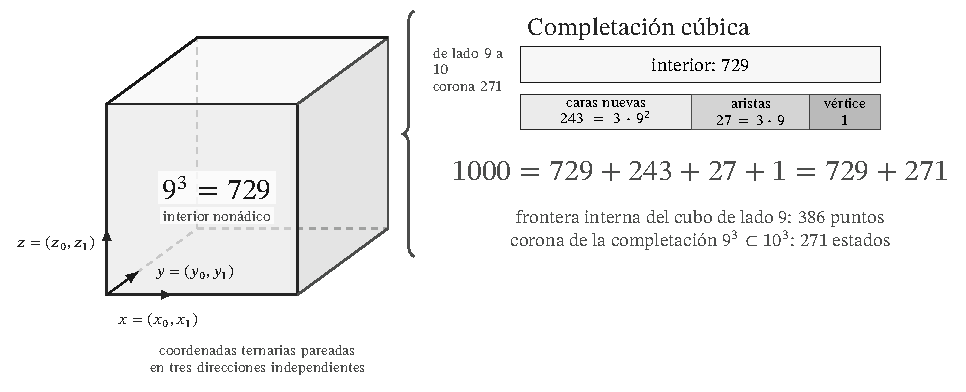
\includegraphics[width=\linewidth]{figures/cubo_emrh.pdf}
\caption{Representación cúbica de la ampliación de nueve a diez clases por coordenada. Los estratos \(S_1,S_2,S_3\) sitúan las incidencias añadidas en caras, aristas y ápice; sus cardinales forman la corona de \(271\) elementos. La frontera de \(386\) elementos pertenece al cubo inicial. La perspectiva geométrica complementa la partición de la figura~\ref{fig:revision-emrh}; las separaciones gráficas tienen función esquemática.}
\label{fig:completacion-cubo-recuperado}
\end{figure}


\subsubsection{Conservación de la unidad y compatibilidad dimensional}

La normalización no se limita a dividir una identidad aislada. En dimensión
\(d\), el producto \(\widehat E^d\) lleva la medida uniforme
\(\mu_d(\{x\})=10^{-d}\). La proyección coordenada
\(p_d:\widehat E^{d+1}\to\widehat E^d\) suprime la última coordenada.

\begin{proposition}[Compatibilidad proyectiva de las medidas normalizadas]
Para todo \(d\geq1\),
\[
 (p_d)_*\mu_{d+1}=\mu_d,
 \qquad \mu_d(\widehat E^d)=1.
\]
La masa del estrato con \(r\) coordenadas adicionales es
\(\binom dr9^{d-r}/10^d\), y la suma de las masas de todos los estratos
es uno.
\end{proposition}
\begin{proof}
Cada punto de \(\widehat E^d\) tiene diez preimágenes. Su masa total es
\(10\,10^{-(d+1)}=10^{-d}\). La igualdad para cualquier subconjunto
se obtiene sumando sobre sus puntos. La fórmula estratificada procede
del mismo recuento que \eqref{eq:revision-estratos}; el binomio
\((9+1)^d\) da la normalización total.
\end{proof}

En dimensión tres, retirar el ápice deja masa \(999/1000\), y
restituirlo añade \(1/1000\). Renormalizar antes de la restitución
definiría otra medida: la distinción es operacionalmente relevante.
En particular, conservación de masa probabilística, conservación de los
registros de transporte y disipación termodinámica son afirmaciones con
objetos diferentes. La proposición demuestra la primera y proporciona el
soporte compatible para estudiar la segunda; la tercera requiere una
realización dinámica y energética especificada.

También permanece diferenciada la frontera geométrica interna.
Sobre el representante cartesiano \(\{1,\ldots,9\}^3\), retirar
\(\{2,\ldots,8\}^3\) deja \(386\) puntos. Esta frontera pertenece al
cubo inicial, mientras \(\widehat C\setminus C\) pertenece a su
ampliación. La completación cúbica, la expansión posicional de base mil y
la lectura de incidencia excepcional comparten datos del soporte;
sus mapas respectivos determinan qué información de esos datos utiliza
cada representación.


\subsection{Incidencia cúbica y realización lorentziana}

La completación cúbica aporta una relación entre interior y frontera.
Su geometría puede desarrollarse mediante la incidencia de las seis caras
con los ocho vértices. Etiquetemos las caras por \((i,\varepsilon)\),
\(i\in\{1,2,3\}\), \(\varepsilon\in\{+1,-1\}\), y los vértices por
\(\nu\in\{+1,-1\}^3\). La matriz de incidencia es
\[
 M_{(i,\varepsilon),\nu}=\mathbf1_{\{\nu_i=\varepsilon\}}.
\]
Sean \(u=(1,\ldots,1)^{\mathsf T}\in\RR^6\), \(R_F\) la oposición de
caras y \(P_u=uu^{\mathsf T}/6\), \(P_-=(I-R_F)/2\).

\begin{proposition}[Cociente de incidencia de dimensión cuatro]
El Gramiano de incidencia satisface
\[
 MM^{\mathsf T}=12P_u+4P_-.
\]
Sus autovalores \(12,4,0\) tienen multiplicidades \(1,3,2\).
En consecuencia,
\[
 Q_\square=\RR^6/\ker(MM^{\mathsf T})
 \simeq\RR u\oplus E_-,\qquad E_-=\operatorname{im}P_-.
\]
\end{proposition}
\begin{proof}
Una cara contiene cuatro vértices; dos caras opuestas tienen intersección
vacía, y dos caras distintas no opuestas comparten dos vértices.
La matriz \(12P_u+4P_-\) tiene precisamente esas entradas.
El espacio uniforme tiene dimensión uno; las diferencias entre caras
opuestas generan un espacio de dimensión tres, ortogonal al uniforme.
Su complemento tiene dimensión dos y pertenece al núcleo.
\end{proof}

La descomposición \(1+3\) procede de la incidencia. La elección temporal
se declara mediante la forma bilineal
\[
 B_\square([x],[y])=\langle x,(P_--P_u)y\rangle.
\]
Está bien definida en el cociente, porque ambos proyectores anulan el
núcleo. En la base
\[
 t=[u]/\sqrt6,\qquad
 d_i=[e_{i,+}-e_{i,-}]/\sqrt2,
\]
su matriz es \(\operatorname{diag}(-1,1,1,1)\). Quedan explicitados
el dominio, la descomposición y la convención de signo que producen
la realización de Minkowski. El Gramiano positivo determina el cociente;
la asignación temporal determina la forma indefinida sobre él.

El operador
\[
 W_\square=\sqrt6P_u+\sqrt2P_-,\qquad
 W_\square e_{i,\varepsilon}=t+\varepsilon d_i
\]
envía las seis etiquetas de cara a direcciones nulas, puesto que
\(B_\square(t+\varepsilon d_i,t+\varepsilon d_i)=-1+1=0\).
La inversión de una dirección y la oposición de caras disponen así
de una realización geométrica concreta.

\subsubsection{Soldadura, inversión y subdivisión}

La realización celular utiliza un transporte invertible \(U_m(a)\),
que conserva la forma lorentziana, entre las fibras de los extremos de
una arista dual orientada \(a\), una etiqueta
de cara \(\lambda_m(a)\) y una orientación \(\sigma_m(a)\).
Con \(\ell_m=\ell_0/9^m\), la aplicación de soldadura es
\[
 \beta_m(a)=\ell_m\sigma_m(a)
 W_{\square,s(a)}e_{\lambda_m(a)}.
\]
La inversión compatible satisface
\[
 \beta_m(\bar a)=-U_m(a)\beta_m(a).
\]
Identifiquemos las fibras del origen en dos niveles consecutivos mediante
la isometría de refinamiento declarada. Si los nueve subsegmentos
\(a_1,\ldots,a_9\), de nivel \(m+1\), conservan la etiqueta
y la orientación al ser transportados a esa fibra común, entonces
\begin{equation}
 \beta_m(a)=\sum_{j=1}^9
 U_{m+1}(a_1\cdots a_{j-1})^{-1}\beta_{m+1}(a_j).
 \label{eq:soldadura-refinamiento}
\end{equation}
Cada término transportado equivale a \(\ell_m/9\) por la misma
dirección nula, lo que demuestra la identidad. La hipótesis de
compatibilidad determina qué subdivisiones realizan este refinamiento.
La ecuación reúne dirección, escala y transporte, en lugar de limitar
la correspondencia geométrica a un recuento de dimensiones.

Fijadas además la orientación y la forma lorentziana, la dualidad de
Hodge en \(\Lambda^2Q_\square^*\) satisface \(\star^2=-I\).
En dimensión cuatro, el signo es \((-1)^{2(4-2)+1}=-1\).
Se obtiene una estructura compleja real sobre las dos-formas y,
tras complejificación, los subespacios propios de valores \(+i\) y
\(-i\). La realización electromagnética utilizará este dominio
después de construir la sección electrónica y declarar su acoplamiento.

\subsection{Compatibilidad entre las reducciones modular y posicional}

La base decimal por bloques interviene mediante una división euclídea
que conserva simultáneamente residuo y cociente:
\[
 n=1000q+r,\qquad 0\le r<1000.
\]
Puesto que \(1000\equiv1\pmod9\) y \(1000\equiv1\pmod3\),
\[
 n\equiv q+r\pmod9,\qquad n\equiv q+r\pmod3.
\]
Por tanto, la reducción de un bloque requiere la contribución del
cociente para recuperar la clase del entero. Los números \(0\) y
\(1000\) tienen el mismo resto por \(1000\), pero clases diferentes
por \(9\) y por \(3\). Ésta es una razón operatoria para conservar
la memoria durante el cambio de resolución.

El refinamiento ternario y la determinación de un prefijo decimal
pueden coordinarse mediante un único residuo entero. Si \(N/3^L\)
es un extremo de cilindro y \(D/1000^r\) un extremo decimal, definimos
\[
 A=1000^rN-D3^L.
\]
Al añadir seis símbolos ternarios, \(N'=729N+\nu\),
\(L'=L+6\), con \(0\le\nu<729\). Si el prefijo decimal permanece
fijo, se obtiene
\[
 A'=729A+\nu1000^r.
\]
Si se incorpora además un bloque decimal \(\delta\), entonces
\(D'=1000D+\delta\), \(r'=r+1\), y
\begin{equation}
 A'=729000A+\nu1000^{r+1}-729\delta3^L.
 \label{eq:residuo-dos-bases}
\end{equation}
Ambas identidades se demuestran sustituyendo las definiciones. La
comparación de extremos se reduce así a operaciones enteras que
retienen la contribución de cada prolongación. Esta compatibilidad
es la que permite refinar una región antes de evaluar su coordenada real.

% Incorporación al final de extension.tex; no contiene una sección principal.
% Procedencia: RESULTADO_RECUPERADO; explicitación sectorial de las hipótesis.
% Fuentes leídas: monografía Doble proyección holográfica (cantera editorial),
% manuscrito/local/01_tesis_recuperada.tex y
% manuscrito/generated/algebra_holonomica.tex, especialmente §§1--7 y 21.
% Definición rectora de número: manuscrito/flattened/main_autosuficiente.tex,
% secciones que comienzan en líneas 22137 y 23000 de la cantera de 775 páginas.
% No se adopta su presentación global como prueba de todas las flechas TPK.

\subsection{El número como sección compatible y el valor como lectura}
\label{hist:seccion}

La distinción entre estado y observación permite precisar qué objeto se
prolonga cuando aumenta la resolución. A profundidad \(n\), sea \(X_n\)
el conjunto de estados admisibles producidos por APP--TRIT--TPK. Sus datos
incluyen posición, hojas suma y producto, residuos y cocientes, régimen,
orientación, acarreo, fase, ruta, frontera, memoria y supervivencia. No son
coordenadas independientes: las evaluaciones aritméticas y los transportes
anteriores imponen sus relaciones. Una prolongación conserva esas relaciones
en cada antecedente, aunque añada nuevos pasos y nuevos datos de memoria.
La sección compatible \eqref{hist:limite-inverso} conserva estos
antecedentes; las operaciones de las secciones~\ref{hist:algebra}
y~\ref{hist:doble-varianza} precisan su composición y su refinamiento.

Sean \(r_{m,n}:X_m\to X_n\), para \(m\geq n\), las restricciones de
profundidad, con \(r_{n,n}=\operatorname{id}\) y
\(r_{\ell,n}=r_{m,n}\circ r_{\ell,m}\). Cada restricción conserva el
prefijo y la información ya determinada en él.

\begin{definition}[Sección numérica compatible]
Un número HMT es una historia compatible del sistema de estados:
\begin{equation}
 x=(x_n)_{n\geq0}\in X_\infty:=\varprojlim_n X_n,
 \qquad r_{m,n}(x_m)=x_n.
 \label{hist:limite-inverso}
\end{equation}
Un lector es una operación adicional sobre un dominio especificado de estas
historias. Una cifra es una observación finita; un valor escalar es una
evaluación del lector. El par formado por la sección y su lector constituye
una presentación leída, no una redefinición de la identidad de la sección.
\end{definition}

En el dominio arquimediano \(X_\infty^{\mathrm{Arch}}\), el lector asocia
a cada prefijo un cilindro cerrado, conserva su encajamiento y hace tender
su diámetro a cero. Así determina
\begin{equation}
 \operatorname{ev}_{\mathbb R}:X_\infty^{\mathrm{Arch}}\longrightarrow
 \mathbb R,\qquad
 \{\operatorname{ev}_{\mathbb R}(x)\}=\bigcap_n I_n(x).
 \label{hist:evaluacion}
\end{equation}
La construcción concreta de estos cilindros y la decisión de sus fronteras
se desarrollan en la sección~\ref{sec:generacion}. La definición
\eqref{hist:limite-inverso} no afirma por sí sola que la imagen de
\eqref{hist:evaluacion} sea toda la recta: una afirmación de cobertura
requiere su propio teorema. Tampoco una igualdad de valores establece, sin
un resultado de inyectividad, la igualdad de sus historias. Esta separación
permite hablar de precisión como profundidad conservando la diferencia
entre el antecedente aritmético y su realización escalar.

\subsection{Composición de historias y multiplicador de memoria}
\label{hist:algebra}

Fijemos un sector de estados a profundidad \(n\) y una categoría
\(\mathcal C\) cuyas flechas sean sus historias admisibles. La composición
se escribe \(vu=v\circ u\): primero se recorre \(u\) y después \(v\).
Los pasos elementales proceden de la selección, el transporte y la
actualización del TPK. Una fibra trítica local admite la escritura
\(\mathbb R[J_x]/(J_x^2+\tau(x)1_x)\), donde
\(\tau(x)\in\{+1,0,-1\}\). El régimen y la orientación pertenecen al
estado que se transporta; una transición entre regímenes no equivale a
identificar sus álgebras cuadráticas.

La siguiente formulación precisa un sector algebraico de esa composición.
Para cada objeto \(x\), se da un álgebra real asociativa unitaria \(A_x\),
que puede ser no conmutativa. Para cada \(u:x\to y\), se da un
homomorfismo unital \(\rho_u:A_x\to A_y\). Suponemos una acción estricta:
\begin{equation}
 \rho_{\operatorname{id}_x}=\operatorname{id}_{A_x},\qquad
 \rho_v\rho_u=\rho_{vu}.
 \label{hist:accion-estricta}
\end{equation}
Para cada pareja componible \(u:x\to y\), \(v:y\to z\), fijamos un
multiplicador central invertible
\(\Omega(v,u)\in Z(A_z)^\times\). Se exige la normalización
\(\Omega(\operatorname{id}_y,u)=\Omega(u,\operatorname{id}_x)=1_y\)
y, para cada triple componible, la identidad
\begin{equation}
 \rho_w\bigl(\Omega(v,u)\bigr)\Omega(w,vu)
   =\Omega(w,v)\Omega(wv,u).
 \label{hist:cociclo}
\end{equation}
Son hipótesis explícitas sobre los transportes y sus coeficientes, no una
consecuencia de llamar holonómica a la dinámica. Al aplicar esta presentación
a un sector TPK deben identificarse sus \(\rho_u\) y \(\Omega(v,u)\).
Las transiciones expresadas mediante bimódulos requieren conservar esa
estructura y no quedan reemplazadas por \eqref{hist:accion-estricta}.

El espacio de sumas finitas
\[
 \mathcal H(\mathcal C,A,\rho,\Omega)
   =\bigoplus_{u\in\operatorname{Mor}(\mathcal C)} A_{t(u)}T_u
\]
recibe el producto bilineal
\begin{equation}
 (aT_v)(bT_u)=a\rho_v(b)\Omega(v,u)T_{vu},
 \label{hist:producto}
\end{equation}
si las flechas son componibles, y cero en otro caso. Aquí \(t(u)\)
designa el estado terminal. La suma reúne historias con coeficientes; el
producto concatena historias conservando el multiplicador del registro.

\begin{proposition}[Asociatividad sectorial con multiplicador central]
Bajo \eqref{hist:accion-estricta} y \eqref{hist:cociclo}, el producto
\eqref{hist:producto} es asociativo. Si el conjunto de objetos es finito,
su unidad es \(\sum_x1_xT_{\operatorname{id}_x}\).
\end{proposition}
\begin{proof}
Para \(u:x\to y\), \(v:y\to z\), \(w:z\to t\), sean
\(a\in A_y\), \(b\in A_z\), \(c\in A_t\). Los dos coeficientes
de \(T_{wvu}\) son
\begin{align*}
 ((cT_w)(bT_v))(aT_u):\quad&
 c\rho_w(b)\Omega(w,v)\rho_{wv}(a)\Omega(wv,u),\\
 (cT_w)((bT_v)(aT_u)):\quad&
 c\rho_w(b)\rho_w\rho_v(a)\rho_w(\Omega(v,u))\Omega(w,vu).
\end{align*}
La acción estricta iguala \(\rho_w\rho_v(a)\) con \(\rho_{wv}(a)\).
La centralidad de \(\Omega(w,v)\) permite desplazarlo a la derecha de
ese factor; \eqref{hist:cociclo} iguala entonces los productos restantes.
No se permutan los coeficientes \(a,b,c\). Si el triple no es componible,
ambas parentizaciones son cero por sus estados iniciales y terminales.
La bilinealidad concluye la prueba. Las identidades locales y la
normalización de \(\Omega\) verifican la unidad indicada.
\end{proof}

El acarreo del calendario proporciona un ejemplo efectivo. En la categoría
de un objeto y flechas \(C_9\), tomemos coeficientes
\(A=\mathbb R[z,z^{-1}]\), acción identidad y
\[
 \Omega(b,a)=z^{c_0(a,b)},\qquad
 c_0(a,b)=\left\lfloor\frac{a+b}{9}\right\rfloor,
 \quad 0\leq a,b<9.
\]
Las dos sumas de acarreos de un triple son
\(\lfloor(a+b+c)/9\rfloor\); por ello se cumple
\eqref{hist:cociclo}. La variable formal \(z\) registra la vuelta sin
asignarle un valor numérico. Imponer después \(z^{12}=1\) recupera el
registro dodecafásico del calendario \eqref{eq:extension108}; conservar
\(z\) sin esa relación distingue vueltas sucesivas. El ejemplo realiza
la memoria de este calendario, sin identificarla con la totalidad de la
memoria TPK.

\subsection{Doble varianza del refinamiento y conservación de la unidad}
\label{hist:doble-varianza}

Al restringir estados se prolongan observables en sentido contrario.
Consideremos las álgebras de funciones, con producto puntual,
\(D_n=\operatorname{Fun}(X_n,\mathbb R)\). La precomposición define
\begin{equation}
 r_{m,n}^*:D_n\longrightarrow D_m,
 \qquad r_{m,n}^*f=f\circ r_{m,n}.
 \label{hist:precomposicion}
\end{equation}
Son morfismos unitales; son además inyectivos cuando las restricciones
correspondientes son sobreyectivas. El límite directo
\(D_{\mathrm{cyl}}=\varinjlim_n(D_n,r_{n+1,n}^*)\) reúne las
observaciones de profundidad finita. No se identifica aquí este álgebra
con toda el álgebra de rutas: prolongar los operadores de transporte exige
también sus compatibilidades con el refinamiento.

\begin{lemma}[Unidad y naturalidad de la evaluación]
Si \(e_x\) es el indicador de \(x\in X_n\), se cumple
\begin{equation}
 r_{m,n}^*e_x=\sum_{y:\,r_{m,n}(y)=x}e_y,
 \qquad r_{m,n}^*1_n=1_m,
 \label{hist:unidad}
\end{equation}
y, para todo \(f\in D_n\), \(y\in X_m\),
\[
 \langle r_{m,n}^*f,y\rangle=\langle f,r_{m,n}y\rangle.
\]
Cada sección \(x\in X_\infty\) determina una evaluación bien definida
\(D_{\mathrm{cyl}}\to\mathbb R\), dada por \([f]\mapsto f(x_n)\)
para \(f\in D_n\).
\end{lemma}
\begin{proof}
Las fibras de \(r_{m,n}\) forman una partición de \(X_m\). Sus
indicadores son ortogonales y suman \(1_m\), lo que prueba
\eqref{hist:unidad}. La naturalidad es la definición de precomposición.
Finalmente, \((r_{m,n}^*f)(x_m)=f(x_n)\), de modo que dos representantes
compatibles dan la misma evaluación en el límite directo.
\end{proof}

La unidad global es la función constante uno sobre todas las posibilidades;
la sección individual selecciona una historia compatible. Conservar la
primera no significa inmovilizar la segunda. El refinamiento puede aumentar
la cantidad de extensiones y la profundidad de cada historia manteniendo
la unidad y todas las evaluaciones de sus antecedentes.

\subsection{Retorno de fase, representación de Weyl y dos lecturas}
\label{hist:puente-lecturas}

La ley \eqref{eq:holonomia-memoria} adquiere una realización operatoria
en la suspensión bilateral que se construirá en la
sección~\ref{sec:generacion}. Allí \(T\) es el avance de un paso,
\(V_9\) observa la fase nonádica, \(W_\delta\) la fase de rotación y
\(D_M\) el grado de memoria. Escribiendo
\(\widehat\Gamma_9=T^9\) para la vuelta en esta representación,
las relaciones de Weyl \eqref{eq:weyl-relojes} implican, sobre vectores
de soporte finito,
\begin{equation}
 \begin{aligned}
 V_9\widehat\Gamma_9&=\widehat\Gamma_9V_9,\qquad
 W_\delta\widehat\Gamma_9=e^{2\pi i9\delta}
     \widehat\Gamma_9W_\delta,\\
 [D_M,\widehat\Gamma_9]&=\widehat\Gamma_9.
 \end{aligned}
 \label{hist:tres-retornos}
\end{equation}
La primera igualdad sigue de \(\zeta_9^9=1\); la segunda, de nueve
aplicaciones de la covariancia de \(W_\delta\); la tercera expresa
el incremento unitario de memoria. La fase finita retorna, mientras la
rotación irracional y la memoria distinguen el estado siguiente. Los
caracteres y el parámetro \(\delta\) se realizan después desde la
construcción numérica allí especificada: no seleccionan retrospectivamente
las semillas. Esta representación describe observables y traslaciones de
la suspensión; no reemplaza todas las coordenadas ni todos los operadores
del TPK.

La doble lectura prolonga la misma distinción entre historia y observable.
En su dominio arquimediano se aplica \eqref{hist:evaluacion}; en el
dominio incidencial calibrado, los mapas \(Q_n\) de la
sección~\ref{exc:doble-lectura} conservan las palabras y los marcos de
frontera. La igualdad allí demostrada
\(r_{n,m}Q_n=Q_mp_{n,m}\) determina su prolongación \(Q_\infty\).
Sobre el dominio común de ambas lecturas pueden considerarse conjuntamente
\(\operatorname{ev}_{\mathbb R}(x)\) y \(Q_\infty(x)\): la
primera retiene el valor; la segunda, la incidencia transportada que su
codominio conserva. La sección antecede a ambas. Esta articulación permite
pasar de la aritmética de historias a las constantes y a la lectura
excepcional sin convertir sus realizaciones en nuevos datos iniciales.


\clearpage
\section{Construcción correlativa del continuo: historias, transporte, incidencia y terminal}
\label{iv:continuo-conjunto}
La aritmética expresada por una forma normal conserva una lectura precisa del estado que la produce. Para situar esa lectura dentro de HMT es necesario mantener también las historias, las hojas y las operaciones que actúan sobre ellas. Este capítulo reúne ese sustrato común. Sus distintas construcciones se obtienen del mismo árbol de ejecuciones APP–TRIT–TPK; los cortes de exposición permiten estudiar sus propiedades sin convertirlas en dominios independientes elegidos por una aplicación posterior.

El punto de partida es el núcleo formal expuesto anteriormente. Una emisión admisible contiene la operación de APP, la orientación del TRIT, el cambio de hoja, el residuo y el cociente, junto con la actualización efectiva de memoria del TPK. Cuando se expresa solamente un residuo, la historia de ejecución sigue perteneciendo al objeto de partida. Dos ejecuciones con idéntica lectura final no se identifican por ese solo motivo.

\subsection{Historias admisibles y memoria por composición}
\label{iv:cont:historias}
Sea \(X_k\) el conjunto de historias admisibles de longitud \(k\). Sus elementos se construyen por emisiones sucesivas desde el dominio inicial del núcleo. Escribimos \(h\varepsilon\) para la prolongación de \(h\) por una emisión admisible \(\varepsilon\), y \(\rho_k(h\varepsilon)=h\) para la supresión de la última emisión. Se conserva la etiqueta de la emisión, incluso cuando diferentes etiquetas producen un mismo estado expresado.

En las dos hojas aritméticas, los datos locales satisfacen las divisiones exactas

\[
\delta_\diamond=r_\diamond+9q_\diamond,
\qquad 0\leq r_\diamond<9,
\qquad \diamond\in\{\Sigma,\Pi\}.
\]
La coordenada orientada del TRIT admite, análogamente, una escritura \(\Delta=o_r+3\kappa\), con el representante orientado declarado por el núcleo. La conservación del cociente permite componer esas representaciones sin sustituir una emisión por su residuo aislado.

En una coordenatización de memoria, la actualización de una emisión se escribe

\[
U_\varepsilon(m)=C_\varepsilon m+\kappa_\varepsilon.
\]
Para una trayectoria \(\alpha=(\varepsilon_1,\ldots,\varepsilon_k)\), la operación efectiva es la composición ordenada de esas actualizaciones. Su parte lineal y su traslación son

\[
C_\alpha=C_{\varepsilon_k}\cdots C_{\varepsilon_1},
\qquad
\kappa_\alpha=
\sum_{j=1}^{k}C_{\varepsilon_k}\cdots
C_{\varepsilon_{j+1}}\kappa_{\varepsilon_j}.
\]
El producto vacío de la última suma es la identidad.

\begin{proposition}[Compatibilidad afín de la concatenación]
\label{iv:cont:concatenacion}
Si \(\alpha\) precede a \(\beta\), entonces

\[
C_{\beta\alpha}=C_\beta C_\alpha,
\qquad
\kappa_{\beta\alpha}=C_\beta\kappa_\alpha+\kappa_\beta,
\qquad
U_{\beta\alpha}=U_\beta U_\alpha.
\]
\end{proposition}
\begin{proof}
Sustituir \(U_\alpha(m)\) en \(U_\beta\) produce \(C_\beta C_\alpha m+C_\beta\kappa_\alpha+\kappa_\beta\). La descomposición en parte lineal y traslación da las tres identidades. La asociatividad de la composición demuestra que el resultado no depende de una subdivisión auxiliar de la trayectoria.
\end{proof}

Esta identidad de cociclo es el contenido preciso de la memoria acumulada. La cantidad transportada por una segunda trayectoria depende de la actualización de coordenatización que ésta realiza; no es, en general, la suma sin transporte de dos registros.

El retorno nonádico conserva una segunda distinción. En las coordenadas de fase y vuelta, con \(\bar r\in\{0,\ldots,8\}\), su representación es

\[
\sigma_9(w,r)=
\left(w+\left\lfloor\frac{\bar r+1}{9}\right\rfloor,
r+1\pmod9\right),
\qquad
\sigma_9^9(w,r)=(w+1,r).
\]
Durante nueve pasos se produce exactamente un cruce de \(8\) a \(0\). La fase retorna y la coordenada de vuelta aumenta. La holonomía enriquecida retiene además las actualizaciones de memoria que acompañan ese recorrido.

\subsection{Refinamiento del árbol y medida de historias}
\label{iv:cont:medida}
Se fija el conjunto inicial finito no vacío de semillas admisibles, con una masa inicial estrictamente positiva y de suma \(1\). En este apartado cada historia tiene un número finito y positivo de prolongaciones. La supresión de emisiones define las aplicaciones de refinamiento. La admisibilidad del núcleo proporciona las prolongaciones; cuando una residencia utiliza una emisión neutra, ésta da explícitamente una sección de \(\rho_k\). La existencia de esa sección se refiere al árbol que incluye dicha emisión, no a cualquier restricción arbitraria de rutas.

Sea \(d(h)\geq1\) el número de emisiones admisibles en \(h\). La elección equiprobable entre sus sucesores define

\[
\mu(h\varepsilon)=\frac{\mu(h)}{d(h)}.
\]
Más generalmente, una distribución local positiva \(p(\varepsilon\mid h)\), cuya suma es \(1\), define \(\mu(h\varepsilon)=\mu(h)p(\varepsilon\mid h)\). Esta segunda formulación permite conservar las ponderaciones del lector cuando los números de prolongaciones no son uniformes.

\begin{proposition}[Compatibilidad cilíndrica y esperanza condicional]
\label{iv:cont:esperanza}
En cada nivel se cumple

\[
\sum_{\rho_k(y)=x}\mu(y)=\mu(x).
\]
En los espacios \(L^2(X_k,\mu_k)\), las aplicaciones

\[
(J_kf)(y)=f(\rho_k(y)),
\qquad
(E_kg)(x)=\sum_{\rho_k(y)=x}\frac{\mu(y)}{\mu(x)}g(y)
\]
satisfacen \(E_k=J_k^*\), \(E_kJ_k=I\) y \(\|J_kf\|=\|f\|\).

\end{proposition}
\begin{proof}
La primera identidad es la normalización de las probabilidades locales. Aplicándola a \(|f(x)|^2\) se obtiene la isometría. Al agrupar por predecesores la suma que define \(\langle J_kf,g\rangle\), se obtiene la fórmula de \(E_k\); sobre una función constante en cada fibra, esa fórmula devuelve su valor.
\end{proof}

Las masas compatibles definen una medida de probabilidad sobre el espacio de historias infinitas: el cilindro de una historia finita recibe su masa \(\mu(h)\). La medida se extiende desde la álgebra de cilindros, y su unicidad procede de que éstos generan la sigma-álgebra. Si el árbol es finitamente ramificado y cada historia tiene una prolongación, el límite inverso de sus niveles por supresión de emisiones es no vacío. En la topología cilíndrica, cada cilindro no vacío tiene medida positiva.

Esta medida distingue historias que convergen a una misma representación. La medida uniforme sobre valores terminales sería una lectura distinta, pues eliminaría las multiplicidades que la construcción acaba de conservar.

\subsection{Transporte por hojas y contabilidad exacta de las salidas}
\label{iv:cont:transporte}
Consideremos primero el espacio con base ortonormal formada por las historias del nivel \(k\). El transporte que conserva la etiqueta de cada prolongación es

\[
\mathcal U_ke_h=
\sum_{\varepsilon\ \mathrm{admisible\ en}\ h}
\sqrt{p(\varepsilon\mid h)}\,e_{h\varepsilon}.
\]
Los conjuntos de sucesores de predecesores distintos son disjuntos. La normalización de \(p\) demuestra, por tanto, \(\mathcal U_k^*\mathcal U_k=I\). La representación mediante masas de historias se relaciona con ésta por el cambio de base diagonal que incorpora \(\sqrt{\mu(h)}\).

La etiqueta de hoja forma parte del registro completo de una historia. Se escribe
\[
\widehat h=((h_0,s_0),\ldots,(h_k,s_k)),\qquad
s_j\in\{\Sigma,\Pi\},
\]
donde \(s_j\) es la hoja activa en el paso \(j\). La prolongación añade la emisión y la hoja \(s_{k+1}\) que determina el selector operativo del TPK, conservando íntegro el prefijo, incluida la hoja inicial. En la base de esas historias levantadas,
\[
\mathcal U_ke_{\widehat h}
=\sum_{\varepsilon\ \mathrm{admisible\ en}\ \widehat h}
\sqrt{p(\varepsilon\mid\widehat h)}\,e_{\widehat h\varepsilon},
\qquad
P_ke_{\widehat h}=\mathbf1_{s_k=\Sigma}e_{\widehat h},\quad
Q_k=I-P_k.
\]
Así, \(P_k\) lee la hoja actual, mientras la distinción entre historias se mantiene por su prefijo completo. Dos historias iniciales que lleguen a la misma hoja activa siguen teniendo sucesores distintos. La prueba de isometría por colecciones disjuntas de prolongaciones se aplica literalmente a esta base.
La orientación trítica es otra coordenada del registro: el valor \(0\) conserva la lectura de umbral en cada hoja y no añade una tercera hoja a esta descomposición. Separamos ahora la conservación de hoja y el intercambio de hoja:

\[
A_k=P_{k+1}\mathcal U_kP_k+Q_{k+1}\mathcal U_kQ_k,
\qquad
\eta_k=Q_{k+1}\mathcal U_kP_k+P_{k+1}\mathcal U_kQ_k.
\]
\begin{proposition}[Identidad de Gram por hojas]
\label{iv:cont:gram}
Para un transporte lineal \(U\), sea o no isométrico, la descomposición anterior satisface

\[
A^*A+\eta^*\eta=PU^*UP+QU^*UQ.
\]
En particular, para \(U=\mathcal U_k\),

\[
A_k^*A_k+\eta_k^*\eta_k=I.
\]
\end{proposition}
\begin{proof}
En \(A^*A\) y \(\eta^*\eta\), los términos mixtos que contienen \(P_{k+1}Q_{k+1}\) se anulan. Al sumar los términos restantes aparece \(P_kU^*(P_{k+1}+Q_{k+1})UP_k\), y su análogo con \(Q_k\). La primera identidad resulta de la complementariedad de los proyectores; la segunda utiliza además \(U^*U=I\).
\end{proof}

La primera identidad es la fórmula general. Sustituir su lado derecho por \(U^*U\) requiere que los bloques cruzados de ese Gram se anulen. La conservación isométrica del transporte de historias proporciona aquí esa condición; no debe atribuirse automáticamente a una compresión posterior.

Escribamos \(F_{0,0}=I\), \(F_{0,n}=A_{n-1}\cdots A_0\) y \(T_N=F_{0,N}^*F_{0,N}\).

\begin{theorem}[Descomposición finita con residuo terminal]
\label{iv:cont:terminal}
Para cada horizonte \(N\),

\[
I=\sum_{n=0}^{N-1}
F_{0,n}^*\eta_n^*\eta_nF_{0,n}+T_N.
\]
La sucesión \(T_N\) es positiva y decreciente, y posee un límite fuerte positivo \(T_\infty\). La suma de salidas converge fuertemente a \(I-T_\infty\).

\end{theorem}
\begin{proof}
La proposición~\ref{iv:cont:gram} da \(T_n-T_{n+1}=F_{0,n}^*\eta_n^*\eta_nF_{0,n}\). La suma telescópica prueba la igualdad finita y la monotonía. Para cada vector, las formas cuadráticas decrecen a un límite; la polarización define una forma acotada positiva y, por el teorema de representación de formas acotadas, un operador \(T_\infty\). La convergencia es fuerte porque, para un operador positivo \(S\leq I\), \(\|Sv\|^2\leq\langle v,Sv\rangle\); se aplica a \(S=T_N-T_\infty\).
\end{proof}

El residuo terminal se conserva hasta demostrar su extinción en el dominio considerado. Esta distinción impide que un retorno de fase, por sí solo, se convierta en una hipótesis de agotamiento de todas las historias.

\subsection{Balance orientado y cancelación en el refinamiento}
\label{iv:cont:balance}
Una historia lleva su orientación acumulada \(o(h)\) y los recuentos de sus visitas a las dos hojas. El balance local correspondiente es

\[
b(h)=o(h)\bigl(N_\Sigma(h)-N_\Pi(h)\bigr),
\qquad
b^+=\frac{|b|+b}{2},\quad b^-=\frac{|b|-b}{2}.
\]
Cuando un lector expresa la media sobre las prolongaciones, se define \(b_c=Eb_f\). La orientación sigue estando en el argumento de \(b_f\); no se elimina antes de promediar.

\begin{proposition}[Defecto exacto de cancelación]
\label{iv:cont:cancelacion}
La cantidad

\[
\kappa_{\mathrm{can}}=
\frac{E|b_f|-|Eb_f|}{2}
\]
es no negativa y satisface

\[
E(b_f^+)=(b_c)^++\kappa_{\mathrm{can}},
\qquad
E(b_f^-)=(b_c)^-+\kappa_{\mathrm{can}}.
\]
\end{proposition}
\begin{proof}
La desigualdad triangular ponderada da \(|Eb_f|\leq E|b_f|\). Al escribir las partes positiva y negativa mediante \((|b|\pm b)/2\), se obtienen ambas igualdades.
\end{proof}

La información omitida al expresar solamente el balance es la cancelación común de las contribuciones opuestas. Esta cantidad se determina desde las mismas prolongaciones utilizadas por el transporte anterior. El factor \(1/9\) aparece sólo cuando la fibra contiene nueve sucesores con pesos iguales; la esperanza condicional es la regla que sigue siendo válida para ramificación y ponderaciones generales.

\subsection{Incidencia ternaria de las hojas y complejo rectangular}
\label{iv:cont:incidencia-rectangular}
Las dos hojas determinan el módulo \(V=\mathbb F_3e_\Sigma\oplus\mathbb F_3e_\Pi\). Sus cuatro direcciones proyectivas son las rectas generadas por \(e_\Sigma,e_\Pi,e_\Sigma+e_\Pi,e_\Sigma-e_\Pi\). De ellas proceden seis pares no ordenados. Los ocho vectores no nulos son sus representantes orientados. Así, los recuentos \(4,6,8\) pertenecen a operaciones distintas sobre un mismo módulo de hojas.

Sobre las seis posiciones de pares, definimos

\[
(Ba)_{\{L,L'\}}=a_L+a_{L'},
\qquad
s(q)=\sum_{\{L,L'\}}q_{\{L,L'\}}.
\]
Cada dirección interviene en tres pares; por ello \(sB=0\) en \(\mathbb F_3\). El lector \(W(q)=\mathbf1_{s(q)=0}-1/3\) es invariante bajo \(q\mapsto q+Ba\). Sobre el ambiente uniforme \(\mathbb F_3^6\), sus momentos son

\[
\mathbb EW=0,\qquad
\mathbb EW^2=\frac29,\qquad
\mathbb EW^3=\frac2{27}.
\]
En efecto, \(s\) es sobreyectiva y cada fibra contiene \(3^5\) elementos. El lector vale \(2/3\) con probabilidad \(1/3\) y \(-1/3\) con probabilidad \(2/3\). Estas medias describen el ambiente uniforme; la distribución inducida por un subconjunto de historias debe calcularse con sus propias multiplicidades, ya conservadas en \(X_k\).

Para fijar los puertos sin perder multiplicidades, a profundidad \(k\) se conservan las lecturas etiquetadas \(\lambda_\Sigma(h)=(h,\Sigma)\) y \(\lambda_\Pi(h)=(h,\Pi)\). Sus conjuntos son
\[
I_k=\{\lambda_\Sigma(h):h\in X_k\},\qquad
J_k=\{\lambda_\Pi(h):h\in X_k\}.
\]
Son finitos y no vacíos porque lo es \(X_k\). Los valores, cocientes y residuos se expresan sobre esos puertos; una igualdad de valores no identifica sus etiquetas. El producto \(I_k\times J_k\) es el dominio de la lectura rectangular, dentro del cual se registra el soporte de las incidencias admisibles.

Fijado este nivel, escribimos \(I=I_k\), \(J=J_k\) y \(A_N=\mathbb Z/3^N\mathbb Z\). Elegimos puertos de referencia \(i_0,j_0\). Esta elección sólo proporciona coordenadas para las fórmulas de reconstrucción. Las aplicaciones

\[
\kappa(u,v)_{ij}=u_i-v_j,
\qquad
(\delta w)_{ij}=w_{ij}-w_{ij_0}-w_{i_0j}+w_{i_0j_0}
\]
definen la siguiente secuencia, válida sobre el anillo finito \(A_N\):

\[
0\longrightarrow A_N\longrightarrow
A_N^I\oplus A_N^J\mathrel{\mathop{\longrightarrow}^{\kappa}}
A_N^{I\times J}\mathrel{\mathop{\longrightarrow}^{\delta}}
A_N^{(I\setminus\{i_0\})\times(J\setminus\{j_0\})}
\longrightarrow0.
\]
\begin{proposition}[Exactitud de la incidencia rectangular]
\label{iv:cont:rectangular-exacta}
La secuencia anterior es exacta, con primera flecha dada por la diagonal constante.

\end{proposition}
\begin{proof}
La igualdad \(u_i-v_j=0\) para cada par obliga a que todas las coordenadas de \(u\) y \(v\) sean una misma constante. La sustitución directa da \(\delta\kappa=0\). Si \(\delta w=0\), tómense \(u_i=w_{ij_0}\) y \(v_j=w_{i_0j_0}-w_{i_0j}\). Entonces \(u_i-v_j=w_{ij}\). Finalmente, cualquier matriz del último término se prolonga con fila y columna de referencia nulas; su imagen por \(\delta\) es la matriz inicial. La prueba sólo utiliza sumas y restas, por lo que no exige dividir por una unidad del anillo.
\end{proof}

Reducir de \(A_{N+1}\) a \(A_N\), manteniendo fijos \(k,I_k,J_k,i_0,j_0\), conmuta con las dos aplicaciones. Las fórmulas de reconstrucción son las mismas en cada profundidad modular. Ésta es la compatibilidad aritmética demostrada en este apartado. La prolongación de historias \(k\to k+1\) conserva las etiquetas de prefijo; sus aplicaciones entre conjuntos de puertos son un dato distinto del cambio de anillo \(N\to N+1\).

Esas aplicaciones se obtienen de la supresión de emisiones:
\[
\rho_k^\Sigma(h\varepsilon,\Sigma)=(h,\Sigma),\qquad
\rho_k^\Pi(h\varepsilon,\Pi)=(h,\Pi).
\]
Se fija una historia de referencia con prolongaciones compatibles, cuya existencia se demostró para el árbol sin hojas terminales. Sus dos etiquetas definen puertos de referencia compatibles en todos los niveles. El transporte de coordenadas es la precomposición:
\[
(L_ku)_{i'}=u_{\rho_k^\Sigma(i')},\quad
(L_kv)_{j'}=v_{\rho_k^\Pi(j')},\quad
(L_kw)_{i'j'}=w_{\rho_k^\Sigma(i'),\rho_k^\Pi(j')}.
\]
Para el último módulo de la secuencia, se prolonga primero la matriz por cero en la fila y la columna de referencia, se aplica esta misma fórmula y se restringe al nuevo complemento de los puertos de referencia. Esta regla define \(L_k\) también cuando un puerto nuevo tiene por predecesor el puerto marcado.

\begin{proposition}[Naturalidad del complejo rectangular bajo prolongación]
\label{iv:rectangular-natural}
Las aplicaciones anteriores verifican
\(L_k\kappa_k=\kappa_{k+1}L_k\) y
\(L_k\delta_k=\delta_{k+1}L_k\).
Además conmutan con la reducción de coeficientes
\(A_{N+1}\to A_N\) y se componen conforme a la supresión de prefijos.
\end{proposition}
\begin{proof}
La primera identidad se obtiene de
\(u_{\rho_k^\Sigma(i')}-v_{\rho_k^\Pi(j')}\).
En la segunda, cada uno de los cuatro términos que define \(\delta\)
se transporta por la misma precomposición. La compatibilidad de los
puertos marcados identifica sus filas y columnas; cuando un predecesor es
el puerto marcado, los cuatro términos se cancelan y coinciden con
la prolongación por cero. Todas las fórmulas son sumas y restas con
coeficientes enteros, de modo que conmutan con la reducción modular.
La composición de precomposiciones es la precomposición con el
prefijo compuesto, lo que demuestra la última afirmación.
\end{proof}

\subsection{Complejo de memoria y compatibilidad de las incidencias}
\label{iv:cont:memoria}
La misma coordenada acumulada de memoria \(c_y\in\mathbb Z\), en una residencia \(y\), define un complejo libre entero. Su reducción a \(A_N\) utiliza el mismo registro entero antes de reducirlo; por tanto, las profundidades sucesivas son compatibles. Sus generadores son \(f_y\) en grado \(2\), \(e_y,b_y,r_y\) en grado \(1\), y \(g_y\) en grado \(0\):

\[
\partial f_y=3c_y e_y+b_y,\qquad
\partial e_y=g_y,\qquad
\partial b_y=-3c_y g_y,\qquad
\partial r_y=0.
\]
La identidad \(\partial^2=0\) se verifica sobre \(f_y\) mediante \(3c_yg_y-3c_yg_y=0\), y es inmediata en los otros generadores.

Si una trayectoria \(\alpha:y\to y'\) actualiza la memoria, su transporte en el complejo envía los generadores homónimos a sus nuevos representantes, salvo

\[
\Psi_\alpha(b_y)=b_{y'}+3(c_{y'}-c_y)e_{y'}.
\]
\begin{proposition}[Naturalidad del complejo de memoria]
\label{iv:cont:memoria-natural}
Se cumplen \(\partial\Psi_\alpha=\Psi_\alpha\partial\) y \(\Psi_{\beta\alpha}=\Psi_\beta\Psi_\alpha\). Las aplicaciones se prolongan linealmente sobre el anillo de coeficientes elegido.

\end{proposition}
\begin{proof}
Sobre \(f_y\), la imagen de su borde es \(3c_ye_{y'}+b_{y'}+3(c_{y'}-c_y)e_{y'} =3c_{y'}e_{y'}+b_{y'}\). Sobre \(b_y\), el borde de su imagen es \(-3c_{y'}g_{y'}+3(c_{y'}-c_y)g_{y'}=-3c_yg_{y'}\). Los otros dos casos son inmediatos. En una concatenación, las diferencias de memoria se suman telescópicamente, lo que prueba la segunda identidad.
\end{proof}

La relación entre dos representantes de una misma residencia también puede escribirse como un borde explícito. Para una coordenada entera \(v\), reducida en el mismo anillo cuando corresponda, sean

\[
z^-=r_y,\qquad z^+=r_y+3c_yv e_y+v b_y,
\qquad h_*=-vf_y.
\]
Entonces \(\partial h_*=z^--z^+\). Bajo un transporte que actualiza también \(v\), la corrección \(K_\alpha=(v_{y'}-v_y)f_{y'}\) satisface \(K_{\beta\alpha}=K_\beta+\Psi_\beta K_\alpha\). Los símbolos \(K_\alpha\) de esta homotopía local no designan el sello dodecafásico \(K\): pertenecen a otro dominio y su función está especificada por la identidad anterior. Su función puede comprobarse también en la igualdad

\[
z^+_{y'}-\Psi_\alpha z^+_y=\partial K_\alpha.
\]
Ambos miembros valen \((v_{y'}-v_y)(3c_{y'}e_{y'}+b_{y'})\).

\begin{proposition}[Homología y memoria del complejo local]
\label{iv:cont:memoria-homologia}
Sobre \(\mathbb Z\), o después de reducir a \(A_N\), se tiene

\[
H_0(\Gamma)=H_2(\Gamma)=0,
\qquad H_1(\Gamma)\cong A_N[r_y]
\]
en la realización modular, y \(H_1(\Gamma)\cong\mathbb Z[r_y]\) en la realización entera.

\end{proposition}
\begin{proof}
Defínase la homotopía de grado \(1\) mediante \(h(g_y)=e_y\), \(h(b_y)=f_y\), y cero en los otros generadores. Sean \(p\) la proyección al sumando generado por \(r_y\) e \(\iota\) su inclusión. La comprobación sobre cada generador da

\[
\partial h+h\partial=I-\iota p.
\]
En particular, sobre \(b_y\) los términos \(3c_ye_y\) y \(-3c_ye_y\) se cancelan. El complejo se retrae por homotopía al módulo generado por \(r_y\), concentrado en grado \(1\), lo que demuestra la afirmación.
\end{proof}

El transporte \(\Psi_\alpha\) es una cizalla de determinante \(1\). Así, este complejo conserva explícitamente cómo cambia \(c_y\) a nivel de cadenas, pero su homología local no distingue los valores de esa coordenada. La memoria completa permanece en las etiquetas y en los transportes del estado fuente; no se recupera a partir de \(H_1\) aisladamente. Una torsión numérica dependiente de memoria requiere el ensamblaje y la lectura determinantal especificados, además de este complejo local.

\subsection{Ensamblaje con caminos terminales}
\label{iv:cont:ensamblaje}
Para un horizonte finito, las residencias y sus prolongaciones forman una categoría de caminos. A cada residencia \(\nu\) se asigna el módulo libre \(W(\nu)=A_N[\operatorname{Path}(\nu,\mathrm{Term})]\), que conserva cada continuación terminal como generador. Una trayectoria inicial actúa en \(W\) por precomposición. El complejo \(\Gamma(\nu)\) del apartado anterior actúa covariantemente mediante \(\Psi\).

El ensamblaje utiliza ambos transportes en el mismo módulo bigraduado:

\[
\mathcal B_{q,r}=
\bigoplus_{\nu_0\to\cdots\to\nu_q}
W(\nu_q)\otimes_{A_N}\Gamma_r(\nu_0).
\]
Se utiliza el complejo de caminos normalizado: se omiten las cadenas degeneradas que contienen identidades. El horizonte finito acota entonces el número de prolongaciones estrictas y el grado horizontal. El borde horizontal suprime una residencia intermedia componiendo las flechas adyacentes. En el primer extremo transporta \(\Gamma\); en el último precompone \(W\). Con los signos alternados se obtiene el borde de caminos \(d_{\mathrm{bar}}\). El diferencial total es

\[
D=d_{\mathrm{bar}}+(-1)^q\partial_\Gamma.
\]
Las identidades de caras cancelan por pares los términos de \(d_{\mathrm{bar}}^2\). La naturalidad de la proposición~\ref{iv:cont:memoria-natural} implica que \(d_{\mathrm{bar}}\) conmuta con \(\partial_\Gamma\); el factor \((-1)^q\) cancela los términos cruzados del cuadrado. Por tanto, \(D^2=0\). La compatibilidad se demuestra sobre generadores de caminos y no se introduce por una etiqueta de pertenencia a un complejo.

La evaluación terminal tampoco requiere elegir una historia particular. Para cada continuación \(h\), se aplica la composición efectiva de sus actualizaciones. El resultado conserva el par formado por \(h\) y su lectura, con su multiplicidad. Si \(k<\ell<N\), las continuaciones se descomponen como una unión disjunta de prefijos hasta \(\ell\) y sus continuaciones hasta \(N\). La proposición~\ref{iv:cont:concatenacion} demuestra que evaluar directamente o evaluar esas dos partes produce la misma lectura. Así se obtiene el cuadrado de naturalidad del terminal.

Los módulos de caminos, las incidencias, el transporte de memoria y sus diferenciales proceden de las mismas prolongaciones. Su ensamblaje no consiste en añadir a un estado cinco coordenadas que se conservarían por definición: sus relaciones se construyen mediante sumas, bordes y composiciones efectivas, y se verifican sobre sus generadores.

\subsection{Determinantes, límite y lectura aritmética}
\label{iv:cont:determinantes}
En cada residencia, el complejo local libre \(\Gamma\) admite su línea determinante graduada

\[
\operatorname{Det}\Gamma=
\bigotimes_r\left(\bigwedge^{\mathrm{rk}\Gamma_r}\Gamma_r\right)^{(-1)^r}.
\]
El ensamblaje total del apartado anterior tiene, por su parte, los módulos \(\operatorname{Tot}_d\mathcal B=\bigoplus_{q+r=d}\mathcal B_{q,r}\). A horizonte finito y sobre el mismo anillo, son libres de rango finito y sólo un número finito de ellos es no nulo. Su línea es
\[
\operatorname{Det}(\operatorname{Tot}\mathcal B)=
\bigotimes_{q,r}
\left(\bigwedge^{\operatorname{rk}\mathcal B_{q,r}}
\mathcal B_{q,r}\right)^{(-1)^{q+r}}.
\]
Esta fórmula resulta de la descomposición por suma directa en cada grado. Distingue la línea del complejo local y la del ensamblaje con todos los caminos; sus bases se ordenan mediante las etiquetas conservadas. La reducción modular conmuta con estas potencias exteriores porque los módulos y sus bases proceden de los mismos módulos libres enteros a horizonte fijado.
La línea está definida por los módulos y sus grados, tanto sobre \(\mathbb Z\) como después de reducir a \(A_N\); el exponente negativo designa el módulo dual. Una torsión numérica no nula exige, adicionalmente, especificar el complejo sobre un cuerpo, las bases y las identificaciones de homología pertinentes. Para calcular factores de Smith se usa la matriz entera producida antes de la reducción, no un levantamiento arbitrario de una matriz modular. Un bloque cuadrado entero de determinante no nulo es invertible sobre \(\mathbb Q\); su reducción es invertible sobre \(A_N\) solamente cuando ese determinante es una unidad, es decir, cuando no es divisible por \(3\). El refinamiento de memorias e incidencias permite formular y comprobar la estabilidad de los factores invariantes pertinentes; estas condiciones no se deducen de la existencia de la línea determinante.

El paso al límite conserva los proyectivos compatibles de residuos, las historias y sus multiplicidades. Los cuadrados probados en los apartados anteriores permanecen conmutativos porque sus aplicaciones están dadas por las mismas fórmulas en cada nivel. Para una coordenada arquimediana, el paso adicional consiste en expresar intervalos cilíndricos no vacíos, compatibles por inclusión y de diámetro tendente a cero. Sus clausuras compactas anidadas tienen una intersección de un solo punto: la existencia se obtiene por compacidad y la unicidad por la cota del diámetro. Ése es el valor de la lectura límite. Si los intervalos son semiabiertos, el punto puede pertenecer sólo a sus clausuras; la regla de representación de frontera determina entonces su escritura posicional. El valor no sustituye la historia que lo ha producido. La otra representación conserva las incidencias del mismo estado. Los dos destinos comparten su origen sin recibir por ello la misma información.

En los capítulos siguientes, las regiones coinductivas, el registro dodecafásico y la incidencia excepcional se expresan desde ese sustrato con sus respectivos mapas. La realización hilbertiana conserva después las etiquetas de fase y especifica su propia inclusión unital; la dualidad y las pantallas actúan sobre los codominios que allí se construyen. Las operaciones conjuntas aquí reunidas transmiten historias, hojas, orientación y memoria a esas representaciones. La identificación de un funcional concreto con una forma analítica externa requiere, a su vez, escribir su aplicación sobre los generadores y verificar sus productos escalares: las identidades de conservación del presente capítulo no reemplazan esa composición.

\subsection{Procedencia, comprobación y alcance}
\label{iv:cont:mapa-correlativo}
% RESULTADO_RECUPERADO: 04b2_operaciones_intrinsecas_correlativas.tex,
% eq:pdfv2-cor-accion-sp/sol/gau/coh/det y eq:pdfv2-cor-memorias.
% Las marcas internas sp/sol/gau/coh/det corresponden, en ese orden,
% a las cinco filas siguientes; no son cinco dominios independientes.
Las cinco operaciones se reconocen por su acción sobre las mismas
historias y por las relaciones demostradas en los apartados anteriores.
El transporte afín \(U_\alpha\) de la memoria y el transporte
lineal \(\mathcal U_k\) de las historias tienen los dominios
respectivos de las secciones~\ref{iv:cont:historias}
y~\ref{iv:cont:transporte}. La graduación de hojas es
\(\sigma_k=P_k-Q_k\). Para una historia
\(h_j=(\varepsilon_1,\ldots,\varepsilon_j)\), la acumulación del
balance queda explícita mediante
\[
 M_0^\pm=0,\qquad
 M_k^\pm(h_k)=\sum_{j=1}^k b^\pm(h_j),\qquad
 M_{k+1}^\pm(h_k\varepsilon)
 =M_k^\pm(h_k)+b^\pm(h_k\varepsilon).
\]
Cada sumando es la lectura firmada del prefijo correspondiente,
definida en la sección~\ref{iv:cont:balance}. Separar el último
sumando demuestra la actualización; las identidades
\(M_k^+-M_k^-=\sum_{j=1}^kb(h_j)\) y
\(M_k^++M_k^-=\sum_{j=1}^k|b(h_j)|\) se deducen de las
definiciones de las partes positiva y negativa. La acumulación y la
cancelación condicional son, así, operaciones distintas sobre las
mismas contribuciones.

\begin{center}
\small
\begin{tabular}{@{}p{.21\linewidth}p{.48\linewidth}p{.23\linewidth}@{}}
\toprule
Operación conjunta & Objetos y acción efectiva & Desarrollo y prueba\\
\midrule
Transporte y graduación de hojas
& \(\mathcal U_k:\ell^2(\widehat X_k)\to
\ell^2(\widehat X_{k+1})\), con \(\widehat X_k\) formado por
las historias levantadas; \(\sigma_k=P_k-Q_k\), \(A_k\) y
\(\eta_k\) conservan o intercambian la hoja actual.
& Sección~\ref{iv:cont:transporte}; proposición~\ref{iv:cont:gram}
y teorema~\ref{iv:cont:terminal}.\\[5pt]
Balance, cancelación y memoria
& \(b:X_k\to\ZZ\), \(b^\pm:X_k\to\mathbb N_0\);
acumulación \(M_k^\pm\) sobre prefijos y cancelación
\(\kappa_{\mathrm{can}}=(E|b_f|-|Eb_f|)/2\) al expresar
la media condicional.
& Sección~\ref{iv:cont:balance};
proposición~\ref{iv:cont:cancelacion}.\\[5pt]
Incidencia ternaria de las hojas
& \(B:\FF_3^4\to\FF_3^6\),
\((Ba)_{\{L,L'\}}=a_L+a_{L'}\); se conserva el ambiente
completo de \(q\), con \(sB=0\) y \(W(q+Ba)=W(q)\).
& Primera parte de la
sección~\ref{iv:cont:incidencia-rectangular}.\\[5pt]
Puertos y complejo rectangular
& \(\kappa:A_N^{I_k}\oplus A_N^{J_k}\to
A_N^{I_k\times J_k}\), \(\kappa(u,v)_{ij}=u_i-v_j\);
la diferencia \(\delta\) y la precomposición \(L_k\)
conservan las etiquetas y sus multiplicidades.
& Proposiciones~\ref{iv:cont:rectangular-exacta}
y~\ref{iv:rectangular-natural}.\\[5pt]
Memoria celular, relleno y línea determinante
& \(\Psi_\alpha:\Gamma_y\to\Gamma_{y'}\),
\(K_\alpha\in\Gamma_{y',2}\),
\(\partial h_*=z^--z^+\); las líneas
\(\operatorname{Det}\Gamma\) y
\(\operatorname{Det}(\operatorname{Tot}\mathcal B)\)
se forman sobre los complejos basados correspondientes.
& Secciones~\ref{iv:cont:memoria}--\ref{iv:cont:determinantes};
proposiciones~\ref{iv:cont:memoria-natural}
y~\ref{iv:cont:memoria-homologia}.\\
\bottomrule
\end{tabular}
\end{center}

El cuadro identifica cinco acciones de una misma construcción: cada
prefijo conserva sus hojas, orientación, residuos, cocientes, memoria
y prolongaciones terminales. La precomposición de puertos lleva
coordenadas de un nivel al refinado; la reducción de coeficientes
lleva \(A_{N+1}\) a \(A_N\). Sus sentidos y dominios son
distintos y sus cuadrados conmutativos están explicitados en la
proposición~\ref{iv:rectangular-natural}. El ensamblaje de la
sección~\ref{iv:cont:ensamblaje} utiliza simultáneamente las
continuaciones terminales y el transporte del complejo de memoria;
sus fórmulas de composición reúnen las acciones del cuadro sobre el
mismo sistema de historias. La lectura de una línea determinante
como escalar conserva las condiciones de bases, homología y
no singularidad de la sección~\ref{iv:cont:determinantes}.

Este desarrollo reúne las construcciones de estado, árbol y medida
común con las operaciones intrínsecas correlativas. El balance de
\ref{iv:cont:balance}, la secuencia de \ref{iv:cont:rectangular-exacta},
el transporte de memoria de \ref{iv:cont:memoria-natural} y el
ensamblaje de \ref{iv:cont:ensamblaje} dan las identidades de conservación
y composición utilizadas. Las cinco construcciones del continuo se
mantienen como operaciones sobre un mismo árbol. Cada especialización
conserva sus condiciones explícitas: transporte isométrico, pesos uniformes,
extinción del terminal y no singularidad de un bloque determinantal.

El comprobador adjunto contrasta instancias exactas de los cociclos, la cancelación ponderada, la secuencia rectangular y el complejo de memoria. Esos controles acompañan las demostraciones generales del texto y verifican los operadores aquí definidos en sus dominios respectivos. El paso posterior hacia las representaciones excepcionales y la realización hilbertiana conserva sus aplicaciones sobre generadores: la sección~\ref{iv:hilbert} especifica la fibra de fase, los operadores de Weyl y las inclusiones que determinan sus clausuras. La conservación documental y los controles finitos mantienen su función de trazabilidad y contraste de esas pruebas.

\clearpage
\section{Generación coinductiva de \texorpdfstring{\(\pi,\varphi,e\)}{pi, phi, e} a profundidad arbitraria}
\label{sec:generacion}

La emisión de seis bloques es una etapa finita de la construcción, no una expansión decimal completa. Su función consiste en producir regiones con multiplicidad, orientación y reglas de transporte. La prolongación debe conservar esos datos y determinar una colección compatible de prefijos de longitud arbitraria. La palabra \emph{generación} designa esta operación; \emph{genealogía} designa la reconstrucción de sus dependencias. Ambas nociones intervienen, pero cumplen funciones distintas.

\subsection{Órbitas, regiones y caracteres de clausura, propagación y autoescala}

Sobre una palabra \(w=(w_1,\ldots,w_6)\), definimos
\[
 r(w)=(w_3,w_1,w_2,w_5,w_6,w_4),\qquad
 s(w)=(w_4,w_5,w_6,w_1,w_2,w_3).
\]
Se cumple \(r^3=s^2=I\) y \(srs=r^{-1}\); por tanto estas permutaciones realizan el grupo diedral \(D_3\). La acción conserva el catálogo y las multiplicidades y conmuta con \(\Psi\). El cociente de las \(243\) palabras visibles tiene \(43\) órbitas: treinta y ocho de cardinal seis y cinco de cardinal tres.

La clase de clausura se reconoce por un predicado de fibra: sus seis orientaciones tienen cinco emisiones por palabra, multiplicidad total \(1008\) y distribución \(432+4\cdot144\). Existe una sola órbita con esas propiedades en el catálogo. Para precisar las otras dos selecciones, escribimos \(f(w)=\#\Psi^{-1}(w)\), \(m(w)=\sum_{U\in\Psi^{-1}(w)}\operatorname{mult}(U)\) y \(\nu(w)=(n_0,n_1,n_2)\). La clase diagonal aditiva de una emisión es \(d(U)=[i+j]_9\) en los índices de cero a ocho; su firma aditiva conserva esta clase y la orientación \(ES\) o \(NO\). Sea \(\mathcal D(\mathcal O)\) el conjunto de esas clases para todas las emisiones sobre una órbita.

Entre las órbitas de tamaño seis, el predicado conjunto
\[
 f(w)=1,\qquad m(w)=144\quad(w\in\mathcal O),\qquad
 \mathcal D(\mathcal O)=\{0,3,6\}
\]
deja exactamente seis órbitas. En este sector, el censo \(\nu=(2,3,1)\), igual al de clausura, selecciona únicamente la propagación; el censo \(\nu=(2,2,2)\) selecciona únicamente la autoescala. El soporte diagonal no puede omitirse: sin él hay cuatro órbitas unipuntuales equilibradas de multiplicidad \(144\), no una. Finalmente, la existencia de una emisión con \(d=6\) y orientación \(ES\) selecciona un representante de cada órbita y conduce a
\begin{equation}
 w^{\rm cl}=010211,\qquad w^{\rm pr}=201101,\qquad w^{\rm au}=121200.
 \label{eq:palabras-regionales}
\end{equation}
Estos símbolos designan primero regiones del catálogo. La identificación escalar se demostrará mediante sus lectores; no se eligen porque coincidan con cifras de una constante conocida.

La palabra de clausura \(010211\) tiene las cinco preimágenes siguientes:
\begin{center}\small
\begin{tabular}{@{}lll r@{}}\toprule
Emisión de seis bloques&Firma multiplicativa&Papel&Multiplicidad\\\midrule
\(501,614,498,169,272,272\)&\(555555\)&transversal&432\\
\(810,923,870,169,272,272\)&\(339555\)&orientación positiva&144\\
\(810,983,810,169,272,272\)&\(393555\)&orientación positiva&144\\
\(870,923,810,169,272,272\)&\(933555\)&orientación positiva&144\\
\(870,923,810,418,674,521\)&\(933717\)&retorno orientado&144\\\bottomrule
\end{tabular}
\end{center}
La multiplicidad \(432\) y la firma constante \(555555\) caracterizan la región transversal. No identifican la posición central \((5,5)\) de APP. Confundir una firma de seis ventanas con una posición del soporte eliminaría la distinción entre región numérica y estructura electrónica.

La microfibra posee además una morfología bipartita precisa. Cada emisión es un producto de una clase de cursor aditivo y una clase multiplicativa. Las tres regiones positivas comparten la misma clase aditiva de dieciocho condiciones; juntas contienen tres clases multiplicativas de ocho condiciones cada una. La región transversal posee un producto \(18\times24\); las tres positivas reunidas, otro \(18\times24\); y el retorno, un producto \(18\times8\). La descomposición por emisiones tiene cinco partes, mientras la descomposición por componentes conexas del grafo bipartito tiene tres. Ambas conservan las mismas \(1008\) semillas sin reducir la forma a un cardinal.

% BEGIN R27_REG01
\subsection{Incidencias entre mitades de emisiones regionales}
\label{sec:rec27-empalmes}

Sea $\mathcal U_6$ la imagen de las seis ventanas consecutivas del emisor
de \ref{act21:tpk:emision}. Para $u=(u_1,\ldots,u_6)$ definimos
$A(u)=(u_1,u_2,u_3)$ y $B(u)=(u_4,u_5,u_6)$.
El grafo de mitades tiene como vértices esos triples y una arista no
orientada entre $A(u)$ y $B(u)$ por cada emisión.

\begin{proposition}[Ciclo de empalmes regionales]
Los vértices
\[
\begin{aligned}
A&=(830,943,830),&B&=(109,252,252),\\
C&=(810,923,870),&D&=(169,272,272),\\
E&=(850,963,890),&F&=(149,252,212)
\end{aligned}
\]
forman el ciclo $A-B-C-D-E-F-A$.
\end{proposition}
\begin{proof}
Escribimos cada semilla como $(i,j,d)$, con posiciones residuales entre
$0$ y $8$ y direcciones $N=(-1,0)$, $E=(0,1)$ y $S=(1,0)$.
Las siguientes parejas de semillas producen, mediante la recurrencia de
54 instantes, las seis emisiones indicadas:
\[
\begin{array}{c|c|c}
\text{emisión}&s_+&s_\times\\\hline
A\mid B&(0,6,E)&(0,6,N)\\
B\mid C&(0,6,N)&(1,5,E)\\
C\mid D&(0,6,E)&(0,1,S)\\
D\mid E&(0,6,N)&(0,4,S)\\
E\mid F&(0,6,E)&(0,3,E)\\
F\mid A&(0,6,N)&(0,1,S)
\end{array}
\]
Cada fila es un testigo de pertenencia a $\mathcal U_6$, obtenido por
evaluación sucesiva de los dos acumuladores. Al separar cada emisión en
sus dos mitades se obtienen exactamente las seis aristas del ciclo.
\end{proof}

En la clasificación de \eqref{eq:palabras-regionales},
\(A\mid B\), \(C\mid D\) y \(E\mid F\) producen respectivamente
las palabras \(w^{\rm au}\), \(w^{\rm cl}\) y \(w^{\rm pr}\).
Los lectores regionales identifican posteriormente estas salidas con
\(\varphi\), una región de \(\pi\) y \(e\).
Las otras tres emisiones hacen explícito su empalme en el grafo.
El resultado describe incidencias entre salidas del emisor. La realización
temporal de una incidencia utiliza, adicionalmente, la orientación, la fase
y la memoria del estado enriquecido. La incorporación del anclaje APP y
de las cinco regiones de $\pi$ impone condiciones de recorrido adicionales;
el ciclo anterior conserva su función como testigo local de empalme.

El ciclo de seis aristas pertenece a este grafo no dirigido de
semiemisiones. Un recorrido temporal enriquecido conserva además los
datos de anclaje, orientación y cierre de su construcción. La incidencia
entre dos mitades y el transporte de un estado tienen así dominios y
condiciones de composición explícitos.

% END R27_REG01

% BEGIN R28_REGIONAL_CLOSURES_INPUT
% BEGIN R28_REGIONAL_CLOSURES
% Inserción después de REG01. No es un documento autónomo.
% Procedencia: U012_biografia_estructural_pi.tex, líneas 175--324.
% Testigos orientados: verificar_cierres_regionales.py; mismo problema,
% representantes distintos de los paseos impresos en U012.
% Emisor SHA-256: 42fdacab582de8e2d2cb7dfafc6204d200aef01249b3dcc37949e39507f066d8.
\subsubsection{Multigrafo de bloques y cinco cierres regionales mínimos}
\label{regcl27:seccion}

Las \(468\) emisiones del conjunto \(\mathcal U_6\), producidas por
el emisor APP--TRIT--TPK, determinan un multigrafo de bloques. La
identificación de sus anclajes regionales permite resolver un problema
de cobertura conjunta: recorrer las incidencias APP, de propagación,
de autoescala y de cada región de clausura en un mismo paseo cerrado.
El ciclo local de seis empalmes de la sección~\ref{sec:rec27-empalmes}
y estas coberturas conservan sus respectivas condiciones de recorrido.

\paragraph{Grafo de bloques y cociente exacto de fase.}
Para \(U=(U_1,\ldots,U_6)\in\mathcal U_6\), definimos
\begin{equation}
 A(U)=(U_1,U_2,U_3),\qquad B(U)=(U_4,U_5,U_6).
 \label{regcl27:mitades}
\end{equation}
El multigrafo no dirigido \(\widetilde G\) tiene por vértices las ternas
que aparecen como \(A(U)\) o \(B(U)\), y una arista etiquetada por cada
\(U\), incidente en esas dos ternas. Se retienen las \(468\) etiquetas:
dos emisiones distintas no se identifican por compartir extremos, ni
porque una intercambie las mitades de otra.

La fase interna actúa sobre cada terna por rotación cíclica:
\begin{equation}
 (a,b,c)\sim(b,c,a)\sim(c,a,b),\qquad
 \operatorname{can}(a,b,c)
 =\min_{\rm lex}\{(a,b,c),(b,c,a),(c,a,b)\}.
 \label{regcl27:fase}
\end{equation}
El grafo \(G\) sustituye los extremos de la arista \(U\) por
\(\operatorname{can}A(U)\) y \(\operatorname{can}B(U)\), conservando
su etiqueta. La equivalencia actúa exactamente por las tres rotaciones
cíclicas de cada vértice; cada emisión mantiene su identidad como arista.

La enumeración del mismo emisor y la búsqueda de componentes dan
\begin{equation}
\begin{array}{c|r|l}
 & |V|&\text{tamaños de componentes}\\ \hline
 \widetilde G&96&(28,28,28,4,4,4)\\
 G&32&(28,4)
\end{array}
\label{regcl27:componentes}
\end{equation}
Para obtener estos datos se reúnen los extremos distintos, se añade
cada incidencia en ambos sentidos y se recorre por anchura cada
componente aún no visitada. La adyacencia puede deduplicarse para contar
componentes, pero las etiquetas paralelas se conservan al buscar cierres
con aristas prescritas.

\paragraph{Anclaje APP y numeración regional.}
Las tres aristas comunes son
\begin{equation}
\begin{aligned}
 U_{\rm APP}&=903|850|850|252|109|252,\\
 U_e&=850|963|890|149|252|212,\\
 U_\varphi&=830|943|830|109|252|252.
\end{aligned}
\label{regcl27:anclajes}
\end{equation}
Fijamos el extremo
\(v_{\rm APP}=\operatorname{can}A(U_{\rm APP})=850|850|903\).
En las cinco regiones ya construidas se adopta el siguiente orden,
que sitúa la región transversal en la quinta fila:
\begin{equation}
\begin{array}{c|l|c|r}
 i&U_\pi^{(i)}&\rho_i&m_i\\ \hline
 1&810|923|870|169|272|272&++&144\\
 2&810|983|810|169|272|272&++&144\\
 3&870|923|810|169|272|272&++&144\\
 4&870|923|810|418|674|521&--&144\\
 5&501|614|498|169|272|272&\perp&432
\end{array}
\label{regcl27:regiones}
\end{equation}
La numeración distingue las tres regiones \(++\), el retorno mutado
\( -- \) y la transversal \(\perp\). Por ello,
\(\rho=(++ ,++ ,++ ,--,\perp)\) y
\(m=(144,144,144,144,432)\) en este orden; la suma sigue siendo \(1008\).

\paragraph{Cinco testigos completos con sentido de recorrido.}
En cada tabla, la fila \(j\) significa recorrer la arista etiquetada
\(e_j\) desde \(v_{j-1}\) hasta \(v_j\). Los extremos son representantes
canónicos de fase. Como \(G\) es no dirigido, la pareja
\((v_{j-1},v_j)\) fija el sentido de recorrido de la arista etiquetada.
Cada tabla contiene exactamente ocho aristas y satisface
\(v_0=v_8=v_{\rm APP}\).

La búsqueda por anchura descrita en la prueba proporciona los siguientes
testigos, uno para cada conjunto de cuatro aristas objetivo. La
minimalidad se refiere a la longitud; admite varios paseos que la realizan.
\paragraph{Testigo \(i=1\).}
\begin{center}
\small
\begin{tabular}{rlll}
\hline
\(j\)&\(v_{j-1}\)&\(e_j\)&\(v_j\)\\
\hline
1&\(850|850|903\)&\(109|252|252|850|903|850\)&\(109|252|252\)\\
2&\(109|252|252\)&\(109|252|252|810|923|870\)&\(810|923|870\)\\
3&\(810|923|870\)&\(810|923|870|169|272|272\)&\(169|272|272\)\\
4&\(169|272|272\)&\(169|272|272|850|963|890\)&\(850|963|890\)\\
5&\(850|963|890\)&\(850|963|890|149|252|212\)&\(149|252|212\)\\
6&\(149|252|212\)&\(149|252|212|830|943|830\)&\(830|830|943\)\\
7&\(830|830|943\)&\(830|943|830|109|252|252\)&\(109|252|252\)\\
8&\(109|252|252\)&\(903|850|850|252|109|252\)&\(850|850|903\)\\
\hline
\end{tabular}
\end{center}

\paragraph{Testigo \(i=2\).}
\begin{center}
\small
\begin{tabular}{rlll}
\hline
\(j\)&\(v_{j-1}\)&\(e_j\)&\(v_j\)\\
\hline
1&\(850|850|903\)&\(169|272|272|850|903|850\)&\(169|272|272\)\\
2&\(169|272|272\)&\(169|272|272|810|983|810\)&\(810|810|983\)\\
3&\(810|810|983\)&\(810|983|810|169|272|272\)&\(169|272|272\)\\
4&\(169|272|272\)&\(169|272|272|850|963|890\)&\(850|963|890\)\\
5&\(850|963|890\)&\(850|963|890|149|252|212\)&\(149|252|212\)\\
6&\(149|252|212\)&\(149|252|212|830|943|830\)&\(830|830|943\)\\
7&\(830|830|943\)&\(830|943|830|109|252|252\)&\(109|252|252\)\\
8&\(109|252|252\)&\(903|850|850|252|109|252\)&\(850|850|903\)\\
\hline
\end{tabular}
\end{center}

\paragraph{Testigo \(i=3\).}
\begin{center}
\small
\begin{tabular}{rlll}
\hline
\(j\)&\(v_{j-1}\)&\(e_j\)&\(v_j\)\\
\hline
1&\(850|850|903\)&\(169|272|272|850|903|850\)&\(169|272|272\)\\
2&\(169|272|272\)&\(169|272|272|850|963|890\)&\(850|963|890\)\\
3&\(850|963|890\)&\(850|963|890|149|252|212\)&\(149|252|212\)\\
4&\(149|252|212\)&\(149|252|212|870|923|810\)&\(810|870|923\)\\
5&\(810|870|923\)&\(870|923|810|169|272|272\)&\(169|272|272\)\\
6&\(169|272|272\)&\(169|272|272|830|943|830\)&\(830|830|943\)\\
7&\(830|830|943\)&\(830|943|830|109|252|252\)&\(109|252|252\)\\
8&\(109|252|252\)&\(903|850|850|252|109|252\)&\(850|850|903\)\\
\hline
\end{tabular}
\end{center}

\paragraph{Testigo \(i=4\).}
\begin{center}
\small
\begin{tabular}{rlll}
\hline
\(j\)&\(v_{j-1}\)&\(e_j\)&\(v_j\)\\
\hline
1&\(850|850|903\)&\(169|272|272|850|903|850\)&\(169|272|272\)\\
2&\(169|272|272\)&\(169|272|272|850|963|890\)&\(850|963|890\)\\
3&\(850|963|890\)&\(850|963|890|149|252|212\)&\(149|252|212\)\\
4&\(149|252|212\)&\(149|252|212|870|923|810\)&\(810|870|923\)\\
5&\(810|870|923\)&\(870|923|810|418|674|521\)&\(418|674|521\)\\
6&\(418|674|521\)&\(418|674|521|830|943|830\)&\(830|830|943\)\\
7&\(830|830|943\)&\(830|943|830|109|252|252\)&\(109|252|252\)\\
8&\(109|252|252\)&\(903|850|850|252|109|252\)&\(850|850|903\)\\
\hline
\end{tabular}
\end{center}

\paragraph{Testigo \(i=5\).}
\begin{center}
\small
\begin{tabular}{rlll}
\hline
\(j\)&\(v_{j-1}\)&\(e_j\)&\(v_j\)\\
\hline
1&\(850|850|903\)&\(109|252|252|850|903|850\)&\(109|252|252\)\\
2&\(109|252|252\)&\(109|252|252|501|614|498\)&\(498|501|614\)\\
3&\(498|501|614\)&\(501|614|498|169|272|272\)&\(169|272|272\)\\
4&\(169|272|272\)&\(169|272|272|850|963|890\)&\(850|963|890\)\\
5&\(850|963|890\)&\(850|963|890|149|252|212\)&\(149|252|212\)\\
6&\(149|252|212\)&\(149|252|212|830|943|830\)&\(830|830|943\)\\
7&\(830|830|943\)&\(830|943|830|109|252|252\)&\(109|252|252\)\\
8&\(109|252|252\)&\(903|850|850|252|109|252\)&\(850|850|903\)\\
\hline
\end{tabular}
\end{center}

\begin{theorem}[Minimalidad de las cinco coberturas regionales]
\label{regcl27:minimalidad}
Para cada \(i\in\{1,\ldots,5\}\), entre los paseos cerrados de \(G\)
que recorren al menos una vez cada arista de
\[
 E_i^*=\{U_{\rm APP},U_e,U_\varphi,U_\pi^{(i)}\},
\]
la longitud mínima, contada con multiplicidad de recorridos, es ocho.
Se permiten repeticiones de vértices y aristas.
\end{theorem}

\begin{proof}
Todo cierre que recorre \(U_{\rm APP}\) pasa por \(v_{\rm APP}\).
La rotación cíclica de su lista de pasos permite comenzar en ese vértice
sin cambiar longitud ni cobertura. Basta, por tanto, resolver el problema
con origen fijo.

El espacio de búsqueda es el conjunto finito
\[
 \mathscr S_i=V(G)\times\mathcal P(E_i^*),
 \qquad |\mathscr S_i|\le32\cdot16=512.
\]
El estado inicial es \(s_0=(v_{\rm APP},\varnothing)\), y el estado
terminal es \(s_*=(v_{\rm APP},E_i^*)\). Al recorrer una arista \(e\)
incidente en \(v\), hacia su otro extremo \(v'\), se actualiza
\begin{equation}
 (v,M)\longmapsto\bigl(v',M\cup(E_i^*\cap\{e\})\bigr).
 \label{regcl27:transicion-bfs}
\end{equation}
La máscara registra etiquetas de arista, no sólo extremos; de ahí que
no deban colapsarse aristas paralelas distintas.

Todas las transiciones cuestan una unidad. Una cola FIFO, iniciada en
\(s_0\), extrae estados por distancia creciente, marca cada estado en
su primera visita y guarda su predecesor y la etiqueta recorrida.
Equivalentemente, si \(\mathcal F_0=\{s_0\}\), las capas nuevas son
\[
 \mathcal F_{k+1}
 =\operatorname{Succ}(\mathcal F_k)
   \setminus\bigcup_{j=0}^{k}\mathcal F_j.
\]
Por inducción, \(\mathcal F_k\) contiene exactamente los estados cuya
distancia mínima desde \(s_0\) es \(k\). La enumeración finita sobre el
emisor indicado da, para cada una de las cinco regiones,
\[
 s_*\notin\bigcup_{k=0}^{7}\mathcal F_k,\qquad s_*\in\mathcal F_8,
 \qquad (\ell_1,\ell_2,\ell_3,\ell_4,\ell_5)=(8,8,8,8,8).
\]
Las tablas exhiben las cinco cotas superiores, incluyendo las cuatro
etiquetas requeridas en cada caso. La exploración exhaustiva de las
capas anteriores prueba la cota inferior. La combinación prueba la
minimalidad en el problema declarado.
\end{proof}

La longitud ocho caracteriza la cobertura conjunta de cuatro incidencias
en cada región de clausura. El cociente retiene las etiquetas de emisión
y sus empalmes entre clases de fase; la evolución temporal enriquecida
conserva, además, orientación y memoria. Esta descripción enlaza las cinco
regiones con los mismos anclajes de propagación, autoescala y APP, y
complementa el ciclo local de seis empalmes. La prolongación coinductiva
mantiene sus operadores y cilindros junto con esos datos de orientación
y memoria.
% END R28_REGIONAL_CLOSURES

% END R28_REGIONAL_CLOSURES_INPUT

\subsection{Transporte finito y frontera de prolongación}

Los endomorfismos \(L_0,L_1\) del espacio de palabras ternarias actúan antes de la realización arquimediana. Su determinación comienza por las transiciones del estado aritmético, no por la prescripción de dos matrices. Si \(U_t\) es el paso compuesto de selección, transporte y actualización, el bloque observado satisface
\[
 b_j^\chi=\Pi_6(x_j^\chi),\qquad
 x_{j+1}^\chi=U_{9j+9}\cdots U_{9j+1}(x_j^\chi),
 \qquad \chi\in\{\mathrm{cl},\mathrm{pr},\mathrm{au}\}.
\]
Se forman seis transiciones por cada régimen: dos consecutivas en cada una de las tres regiones. Los pares de matrices de orígenes y destinos obtenidos en el registro son
\[
\begin{array}{c|c|c|c}
X_0&Y_0&X_1&Y_1\\\hline
010211&012222&010211&002111\\
012222&010211&002111&110221\\
201101&121221&102011&012222\\
121221&102011&012222&102011\\
121200&112202&121020&010210\\
112202&121020&010210&010200
\end{array}
\]
Cada cadena de seis dígitos representa una fila en \(\FF_3^6\). Puesto que \(\det X_0=1\) y \(\det X_1=-1\) en \(\FF_3\), las ecuaciones \(X_aL_a=Y_a\) determinan unívocamente \(L_a=X_a^{-1}Y_a\). En esa coordenatización de vectores fila resultan
\[
 L_0=\begin{pmatrix}
 2&2&2&1&2&1\\2&1&2&2&1&1\\1&0&0&1&0&2\\
 0&0&1&1&1&0\\2&2&2&0&2&1\\2&1&2&1&0&0
 \end{pmatrix},\quad
 L_1=\begin{pmatrix}
 2&1&2&0&2&2\\1&2&1&1&2&0\\1&2&1&1&1&2\\
 0&1&0&0&2&1\\2&0&2&1&0&1\\0&2&2&2&1&1
 \end{pmatrix}\quad(\bmod3).
\]
El calendario \((L_0,L_0,L_1,L_1)\) produce cuatro nuevos bloques de seis componentes. Sus concatenaciones forman
\[
 w_6\longrightarrow w_{12}\longrightarrow w_{18}
 \longrightarrow w_{24}\longrightarrow w_{30}.
\]
Los subíndices de \(w\) indican longitud acumulada. La frontera \(R_{36}\) conserva la estructura terminal y abre la relación de prolongación; no se renombra como un último bloque periódico que pudiera repetirse indefinidamente.

La identidad \(L=X^{-1}Y\) demuestra unicidad una vez fijadas las transiciones; no sustituye la producción de esas transiciones por \(U_t\). La procedencia de su registro y el examen de los dieciséis calendarios binarios se documentan en el suplemento técnico. El calendario indicado es el único de esos dieciséis que reproduce conjuntamente las tres sucesiones de cinco bloques.

\subsection{Construcción correlacionada y orden de los lectores}
\label{gen:orden-constructor-correlacionado}

El antecedente común de las tres regiones es la emisión aritmética con
su registro de trayectoria. APP proporciona las evaluaciones suma y
producto; TRIT aporta la firma orientada; la transición
\eqref{eq:actualizacion} compone selección de modo, transporte cardinal y
actualización de memoria. El censo de esa emisión produce el catálogo y
sus fibras. Los predicados de multiplicidad, soporte diagonal y orientación
seleccionan los representantes de \eqref{eq:palabras-regionales}.
La correlación regional conserva esta procedencia conjunta, junto con las
incidencias y las restricciones entre sus registros.

Los transportes \(L_0,L_1\) actúan sobre los representantes seleccionados
en la coordenatización fila declarada. El calendario y la concatenación distinguen
la longitud del prefijo, la fase visible y la memoria acumulada. La
coordenada profunda y sus cocientes se explicitan a continuación mediante
\eqref{memprof:division} y \eqref{memprof:inversa}. Las restricciones de
historias se conservan en el sentido de \ref{hist:seccion}.
La selección orientada concreta de \(R_{36}\) tiene su demostración
incidencial en \ref{mg01:frontera}, después de la construcción de \(A_W\);
esa residencia conserva los antecedentes utilizados por su prueba.

Cada lector regional añade una operación tipada al registro que recibe.
En la clausura, el lector simétrico de la pentafibra fija la pendiente
primitiva y la ley de composición determina el compensador de
\eqref{eq:lector-pi}. En la propagación, la composición formal, la unidad
y el generador orientado determinan la recurrencia
\eqref{eq:propagacion}. En la autoescala, el calendario de modos produce
la incidencia \eqref{eq:fav}, cuyo rayo positivo fija la coordenada
normalizada. Las demostraciones siguientes conservan las normalizaciones
y los dominios de estas tres operaciones.

Las cotas racionales y la separación de cilindros evalúan después los
caracteres obtenidos. La emisión posicional efectiva y su compatibilidad
están demostradas en \ref{act21:thm:df-emision-correcta} y
\ref{act21:prop:df-prefijos-compatibles}. El registro dodecafásico conserva
su construcción propia en \ref{act21:chap:despliegue-selector-k};
sus coordenadas y las tres lecturas regionales intervienen posteriormente
en la clausura entera de \ref{sec:alpha}. De este modo, selección de
regiones, transporte, construcción de caracteres y evaluación de prefijos
mantienen sus dominios y su orden, dentro de la misma genealogía
APP--TRIT--TPK.


\subsection{Memoria profunda y compatibilidad de los cilindros}
\label{memprof:seccion}

La prolongación compara estados que conservan simultáneamente residuos,
cocientes y fronteras. En la coordenatización lineal de seis coordenadas del registro,
tomamos el representante entero de \(L_0\) cuyas entradas se han mostrado:
\[
 A_H=\begin{pmatrix}
 2&2&2&1&2&1\\2&1&2&2&1&1\\1&0&0&1&0&2\\
 0&0&1&1&1&0\\2&2&2&0&2&1\\2&1&2&1&0&0
 \end{pmatrix},\qquad\det A_H=1.
\]
La elección de este representante forma parte de la coordenatización: la reducción
módulo tres conserva \(L_0\), mientras que el representante entero fija
la operación sobre los cocientes profundos. Con vectores fila se obtiene
\begin{equation}
 \begin{aligned}
 \mathsf{Div}_H:\mathbb Z^6&\longrightarrow
       \{0,1,2\}^6\times\mathbb Z^6,\\
 x_H&\longmapsto(u_H,x_H^+),\\
 y_H&=x_HA_H,\qquad u_H=[y_H]_3,\qquad
 x_H^+=(y_H-u_H)/3 .
 \end{aligned}
 \label{memprof:division}
\end{equation}
El par \((u_H,x_H^+)\) conserva \(y_H=u_H+3x_H^+\). Puesto que
\(A_H\) es unimodular, su inversa es entera y
\begin{equation}
 x_H=(u_H+3x_H^+)A_H^{-1}.
 \label{memprof:inversa}
\end{equation}
Esta identidad recupera la coordenada profunda desde su residuo y su
cociente. Los otros campos del estado conservan sus registros propios.
La orientación ternaria se lee después mediante
\(0\mapsto0,\ 1\mapsto+1,\ 2\mapsto-1\), manteniendo el residuo
\(u_H\in\{0,1,2\}^6\) y el cociente de \eqref{memprof:division}.

La coordenatización cilíndrica relaciona un prefijo ternario de longitud \(L\), de
índice entero \(N\), con \(k_{\mathrm{dec}}\) tríadas decimales, de
índice \(D\). Los cilindros semiabiertos correspondientes son
\[
 I_3(N,L)=\left[\frac N{3^L},\frac{N+1}{3^L}\right),\qquad
 I_{1000}(D,k_{\mathrm{dec}})
 =\left[\frac D{1000^{k_{\mathrm{dec}}}},
         \frac{D+1}{1000^{k_{\mathrm{dec}}}}\right).
\]
Definimos los enteros de frontera
\[
 a_{\mathrm{cyl}}=N1000^{k_{\mathrm{dec}}}-D3^L,\qquad
 b_{\mathrm{cyl}}=(N+1)1000^{k_{\mathrm{dec}}}-D3^L.
\]
Para un bloque de seis residuos fijamos su codificación entera
\[
 \nu(u_H)=\sum_{j=1}^6(u_H)_j3^{6-j}
 \in\{0,\ldots,728\}.
\]

\begin{lemma}[Actualización entera de los cilindros compatibles]
\label{memprof:cilindros}
Los cilindros anteriores se intersectan si y sólo si
\(a_{\mathrm{cyl}}<3^L\) y \(b_{\mathrm{cyl}}>0\).
Al añadir un bloque ternario de índice
\(\nu\in\{0,\ldots,728\}\), se tiene \(N'=729N+\nu\) y
\(L'=L+6\). Para \(\Delta k_{\mathrm{dec}}\in\{0,1\}\),
las fronteras se actualizan por
\[
 \begin{array}{ll}
 \Delta k_{\mathrm{dec}}=0:
   &a_{\mathrm{cyl}}'=729a_{\mathrm{cyl}}+\nu1000^{k_{\mathrm{dec}}},\\[2pt]
 \Delta k_{\mathrm{dec}}=1:
   &D'=1000D+\delta,\\
   &a_{\mathrm{cyl}}'=729000a_{\mathrm{cyl}}
      +\nu1000^{k_{\mathrm{dec}}+1}-\delta\,729\,3^L ,
 \end{array}
\]
donde \(\delta\in\{0,\ldots,999\}\) es la tríada de la prolongación
compatible. En ambos casos,
\[
 b_{\mathrm{cyl}}'=a_{\mathrm{cyl}}'
          +1000^{k_{\mathrm{dec}}+\Delta k_{\mathrm{dec}}}.
\]
\end{lemma}
\begin{proof}
Dos intervalos semiabiertos se intersectan precisamente cuando cada extremo
izquierdo es menor que el extremo derecho del otro. Multiplicar esas dos
desigualdades por \(3^L1000^{k_{\mathrm{dec}}}\) da
\(a_{\mathrm{cyl}}<3^L\) y \(b_{\mathrm{cyl}}>0\).
La sustitución de \(N'\), \(L'\) y \(D'\) en
\[
 a_{\mathrm{cyl}}'
 =N'1000^{k_{\mathrm{dec}}+\Delta k_{\mathrm{dec}}}-D'3^{L'}
\]
produce las dos recurrencias. Restar las definiciones de
\(b_{\mathrm{cyl}}'\) y \(a_{\mathrm{cyl}}'\) da la última identidad.
\end{proof}

Estas operaciones actúan sobre prefijos enteros y sus restricciones
compatibles. La lectura arquimediana aparece al evaluar el sistema de
cilindros resultante. El dominio de prolongación incorpora además la
orientación, el acarreo, la firma conjunta y los datos de frontera del estado
\(\widehat X\) de \eqref{eq:actualizacion}; la comparación de intervalos
es una componente de esa compatibilidad conjunta.


\subsection{Cinco regiones de clausura y compensación angular}

La región de clausura contiene una componente transversal y cuatro acompañantes. El lector simétrico actúa en el espacio de sus cinco posiciones mediante
\[
 P_5=\frac15\mathbf1\mathbf1^{\mathsf T},\qquad
 \mathbf1=(1,1,1,1,1)^{\mathsf T}.
\]
La invariancia \(P_5\lambda=\lambda\) y la conservación \(\mathbf1^{\mathsf T}\lambda=1\) fuerzan \(\lambda=\mathbf1/5\). Esta normalización distribuye la unidad entre posiciones del lector; no sustituye las multiplicidades de semillas \(432,144,144,144,144\) por frecuencias uniformes. La coordenatización elíptica del lector realiza cada coordenada mediante \(1+\lambda_jJ\); su pendiente es \(\lambda_j\), por lo que la pendiente primitiva resulta \(1/5\). Se hace explícita así la regla que pasa de una coordenada normalizada a una pendiente, en lugar de identificar ambas nociones sin mapa. El lector compone las cuatro posiciones acompañantes por la ley
\begin{equation}
 a\oplus b=\frac{a+b}{1-ab}.
 \label{eq:suma-pendientes}
\end{equation}
Esta ley se obtiene al multiplicar \((1+aJ)(1+bJ)\) en el régimen \(J^2=-I\) y dividir por su componente escalar. Por ello la composición de pendientes es una realización de la estructura cuadrática de TRIT, no una suma ordinaria de cuatro fracciones.

\begin{proposition}[Compensador de la clausura]
La composición de cuatro pendientes \(1/5\) es \(120/119\). La condición de retorno a pendiente uno determina un único compensador positivo de la forma \(1/q\), con \(q>1\), y da \(q=239\).
\end{proposition}
\begin{proof}
La primera duplicación da \((1/5)\oplus(1/5)=5/12\); la segunda, \((5/12)\oplus(5/12)=120/119\). La condición
\[
 \frac{120/119-1/q}{1+(120/119)/q}=1
\]
equivale a \((120-119)q=120+119\), por lo que \(q=239\).
\end{proof}

El carácter de clausura resultante tiene realización
\begin{equation}
 \Pi_{\rm cl}=4\left(4\arctan\frac15-\arctan\frac1{239}\right).
 \label{eq:lector-pi}
\end{equation}
La identidad angular de Machin reconoce \(\Pi_{\rm cl}=\pi\). El sentido de la construcción es preciso: la pendiente y el número de composiciones están declarados por el lector de la pentafibra; la ecuación de compensación fuerza \(239\). Una vez producido este carácter, su evaluación por series alternadas no selecciona de nuevo la órbita de semillas.

Para \(0<x<1\), las sumas alternadas
\[
 A_n(x)=\sum_{j=0}^n\frac{(-1)^jx^{2j+1}}{2j+1}
\]
encierran \(\arctan x\) entre dos truncamientos consecutivos, con diferencia \(x^{2n+3}/(2n+3)\). Aplicadas a las dos pendientes de \eqref{eq:lector-pi}, proporcionan extremos racionales de error explícito. El valor numérico se calcula así como consecuencia del carácter exacto, sin introducir un prefijo objetivo.

\subsection{Lector de propagación y normalización de la unidad}

La región de propagación se realiza mediante una colección formal \(P_t\in\mathcal A[[t]]\), donde \(\mathcal A\) es un álgebra conmutativa unitaria sobre \(\QQ\). Su composición satisface \(P_{t+s}=P_tP_s\), con unidad \(P_0=1\), y el transporte elemental orientado fija el generador escalar \(P'_0=+1\). La condición fija su signo, no sólo su magnitud. Escribiendo
\[
 P_t=\sum_{n\ge0}a_nt^n,
\]
la normalización determina \(a_0=a_1=1\). La comparación del coeficiente de \(s^nt\) en \(P_{s+t}=P_sP_t\) da \((n+1)a_{n+1}=a_na_1\); equivalentemente, \(P'_t=P_t\). Así,
\begin{equation}
 (n+1)a_{n+1}=a_n,\qquad a_n=\frac1{n!}.
 \label{eq:propagacion}
\end{equation}
El carácter en una unidad de parámetro es \(\Pi_{\rm pr}=P_1\), reconocido posteriormente como \(e\).

La normalización del generador importa. La ley semigrupal sin ese dato admitiría \(P_t=e^{ct}\) para distintos \(c\); por ello no se omite la condición que fija la unidad del parámetro en el lector. Esta condición es anterior a la comparación decimal y pertenece a la exposición de la regla operacional, no a la elección de un valor experimental.

\begin{proposition}[Cotas racionales de propagación]
Para \(n\ge1\), sea \(E_n=\sum_{j=0}^n1/j!\). Entonces
\[
 E_n<\Pi_{\rm pr}<E_n+\frac{n+2}{(n+1)(n+1)!}.
\]
\end{proposition}
\begin{proof}
El primer término omitido es \(1/(n+1)!\). Cada cociente posterior es a lo sumo \(1/(n+2)\). La suma geométrica mayorante de la cola es
\[
 \frac1{(n+1)!}\frac1{1-1/(n+2)}
 =\frac{n+2}{(n+1)(n+1)!}.
\]
La desigualdad estricta se sigue de la disminución de los cocientes sucesivos.
\end{proof}

\subsection{Incidencia modal y generación de la autoescala}

El selector trítico produce el ciclo \((+1,-1,0)\). En los modos \(\Sigma,\Pi\), la regla es \(+1:m\mapsto\Sigma\), \(-1:m\mapsto\Pi\), \(0:m\mapsto m\). Con cierre cíclico, el modo observado es \((\Sigma,\Pi,\Pi)\). Sus aristas son \(\Sigma\to\Pi\), \(\Pi\to\Pi\) y \(\Pi\to\Sigma\). Por tanto su incidencia, en ese orden de modos, es
\begin{equation}
 F_{\rm av}=\begin{pmatrix}0&1\\1&1\end{pmatrix}.
 \label{eq:fav}
\end{equation}
Las cuatro entradas se obtienen del calendario, no de una ecuación que haya recibido previamente el valor de \(\varphi\). La repetición del calendario da conteos \(3F_{\rm av},9F_{\rm av},36F_{\rm av}\) en longitudes nueve, veintisiete y ciento ocho. Estos conteos no son las potencias de la matriz.

\begin{theorem}[Carácter positivo de autoescala]
La incidencia \eqref{eq:fav} posee un único rayo propio estrictamente positivo. Al normalizarlo como \((1,x)^{\mathsf T}\), su coordenada \(x\) satisface \(x^2-x-1=0\), \(x>0\), y es \(\varphi=(1+\sqrt5)/2\).
\end{theorem}
\begin{proof}
La ecuación propia da \(x=\lambda\) y \(1+x=\lambda x\). Eliminar \(\lambda\) produce el polinomio. De sus dos raíces sólo una es positiva. Como \(F_{\rm av}^2\) tiene todas sus entradas positivas, el rayo positivo es único y simple. La expresión radical reconoce la coordenada obtenida; no participa en la producción de \(F_{\rm av}\).
\end{proof}

Con \(F_0=0,F_1=1,F_{n+1}=F_n+F_{n-1}\), la incidencia induce, para \(n\geq1\),
\[
 F_{\rm av}^n=\begin{pmatrix}F_{n-1}&F_n\\F_n&F_{n+1}\end{pmatrix}.
\]
Los cocientes consecutivos \(F_{n+1}/F_n\) alternan alrededor de \(\varphi\). La identidad de determinante
\[
 F_{n+1}^2-F_nF_{n+2}=(-1)^n
\]
da una anchura exacta \(1/(F_nF_{n+1})\) entre dos cocientes consecutivos. Su crecimiento hace arbitrariamente pequeña esta horquilla racional.

La medida sobre todas las historias compatibles no coincide con la frecuencia de modos del calendario de tres eventos. La frecuencia cronológica es \((1/3,2/3)\). La medida de máxima entropía del envolvente simbólico definido por \(F_{\rm av}\) se construye con sus vectores propios y tiene razón de pesos \(\varphi^{-2}\). Esta última interviene en la lectura areal--volumétrica; no se obtiene sustituyendo sin más una frecuencia de conteo por otra.

\subsubsection{Espacio de trayectorias y medida invariante entre hojas}
\label{sec:medida-retorno-hojas}

La topología toroidal de APP fija el soporte de las traslaciones cardinales
y sus clases de enrollamiento. La correspondencia entre hojas procede de
otra operación sobre ese mismo soporte: la selección temporal de la
evaluación aditiva o multiplicativa. Su tipado geométrico es
\[
 \eta_{\rm av}(\Sigma)=\mathscr H_{\rm ar},\qquad
 \eta_{\rm av}(\Pi)=\mathscr H_{\rm vol}.
\]
La primera hoja corresponde a la lectura aditiva de frontera; la segunda,
a la lectura multiplicativa de interior. Este mapa transporta las etiquetas
de modo y conserva la incidencia \eqref{eq:fav}. El cuadrado de la razón
de autoescala se determina mediante las trayectorias de esa incidencia.

\Needspace{8\baselineskip}
\begin{definition}[Envolvente simbólico de memoria uno]
Sea
\[
 X_{\rm av}=\{(s_k)_{k\in\mathbb Z}\in
 \{\mathscr H_{\rm ar},\mathscr H_{\rm vol}\}^{\mathbb Z}:
 (F_{\rm av})_{s_k,s_{k+1}}=1\text{ para todo }k\}.
\]
El desplazamiento de índices actúa sobre este espacio. Es el menor sistema
simbólico de memoria uno que contiene las sucesiones modales y conserva
sus pares consecutivos: admite las dos transiciones cruzadas y la
autorretención volumétrica. La fase, la orientación cardinal y los registros
de la trayectoria permanecen en el estado TPK del que se obtiene este
envolvente.
\end{definition}

\begin{proposition}[Ponderación de las trayectorias entre hojas]
En el orden areal--volumétrico, la medida invariante de entropía máxima
de \(X_{\rm av}\) tiene matriz de transición y distribución estacionaria
\begin{equation}
 P_{\rm av}=\begin{pmatrix}0&1\\\varphi^{-2}&\varphi^{-1}\end{pmatrix},
 \qquad
 (\mu_{\rm ar},\mu_{\rm vol})
 =\frac{(1,\varphi^2)}{1+\varphi^2}.
 \label{eq:medida-hojas-exacta}
\end{equation}
En particular, \(\mu_{\rm ar}/\mu_{\rm vol}=\varphi^{-2}\).
\end{proposition}
\begin{proof}
La incidencia ya construida tiene vector propio positivo
\(r=(1,\varphi)^{\mathsf T}\) y autovalor \(\varphi\). La
normalización
\[
 (P_{\rm av})_{ij}
 =\frac{(F_{\rm av})_{ij}r_j}{\varphi r_i}
\]
da la matriz indicada. Sus filas suman uno por
\(\varphi^{-2}+\varphi^{-1}=1\). La simetría de \(F_{\rm av}\)
implica que los pesos proporcionales a \(r_i^2\) satisfacen balance
detallado; por tanto, \(\mu P_{\rm av}=\mu\). La irreducibilidad y la
autorretención volumétrica determinan una única distribución estacionaria.

Para verificar la maximalidad, en toda transición permitida se cumple
\(\log(P_{\rm av})_{ij}=\log r_j-\log r_i-\log\varphi\).
Bajo cualquier medida invariante, los términos de extremo se cancelan
en promedio. Si \(\nu_i\) son sus pesos de vértice y
\(q_i(j)=\nu(s_1=j\mid s_0=i)\), para \(\nu_i>0\), entonces
\[
 h_\nu\leq H_\nu(s_1\mid s_0)
 =\log\varphi-\sum_{i:\nu_i>0}\nu_iD(q_i\Vert P_i)
 \leq\log\varphi,
\]
donde \(D(q\Vert p)=\sum_jq_j\log(q_j/p_j)\) es la entropía
relativa en los pares permitidos y se adopta \(0\log0=0\).
La medida markoviana de \eqref{eq:medida-hojas-exacta} alcanza la cota.
La igualdad en la primera desigualdad exige la propiedad de Markov;
la igualdad en la segunda exige \(q_i=P_i\). La estacionariedad y
la irreducibilidad fijan entonces \(\mu\), lo que establece la
unicidad. Esta es la medida de Parry del envolvente definido.
\end{proof}

La frecuencia \((1/3,2/3)\) cuenta los instantes del calendario primitivo;
\(\mu\) pondera las trayectorias del envolvente. Su razón cuadrática
expresa el producto de las amplitudes de incidencia de entrada y salida.
La memoria y las restricciones de fase del TPK conservan su dominio
propio; la entropía del envolvente corresponde al sistema simbólico
especificado en esta definición.

\subsubsection{Operador de clausura y límite de los retornos marcados}
\label{sec:operador-retorno-marcado}

La coordenada de clausura \(\pi\), generada por el lector regional,
interviene después de la construcción de la incidencia modal. Sean
\(e_{\rm ar}=(1,0)^{\mathsf T}\),
\(e_{\rm vol}=(0,1)^{\mathsf T}\) y
\(P_i=e_ie_i^{\mathsf T}\) los proyectores de hoja. Las condiciones
del lector son conservación de ambas hojas, normalización volumétrica
unitaria y marca areal igual a la coordenada de clausura. Estas condiciones
determinan el operador positivo
\begin{equation}
 D_\pi=\pi P_{\rm ar}+P_{\rm vol}
       =\begin{pmatrix}\pi&0\\0&1\end{pmatrix}.
 \label{eq:operador-marca-pi}
\end{equation}
La diagonalidad expresa la conservación de hojas y las dos entradas
expresan sus normalizaciones; de este modo queda explícita la unicidad
del operador para el lector fijado.

\Needspace{8\baselineskip}
\begin{proposition}[Razón de retornos de frontera]
Para \(n\geq1\), la evaluación marcada
\begin{equation}
 \Theta_n=
 \frac{\langle e_{\rm ar},D_\pi F_{\rm av}^{\,n}e_{\rm ar}\rangle}
 {\langle e_{\rm vol},F_{\rm av}^{\,n}e_{\rm vol}\rangle}
 =\pi\frac{F_{n-1}}{F_{n+1}}
 \label{eq:retorno-marcado-finito}
\end{equation}
satisface
\begin{equation}
 \lim_{n\to\infty}\Theta_n
 =\pi\frac{\mu_{\rm ar}}{\mu_{\rm vol}}
 =\frac{\pi}{\varphi^2}.
 \label{eq:retorno-marcado-limite}
\end{equation}
\end{proposition}
\begin{proof}
Las entradas diagonales de \(F_{\rm av}^{\,n}\) cuentan los caminos
de longitud \(n\) que regresan a su hoja inicial. La fórmula de potencias
ya demostrada proporciona \(F_{n-1}\) y \(F_{n+1}\). El operador
\(D_\pi\) multiplica por \(\pi\) el primer recuento. Finalmente,
\(F_{n-1}/F_{n+1}\) es el producto de dos cocientes consecutivos
que convergen a \(\varphi^{-1}\); su límite es
\(\varphi^{-2}\). La identidad con la razón de pesos se sigue de
\eqref{eq:medida-hojas-exacta}.
\end{proof}

El operador de clausura aparece una sola vez, en la evaluación terminal
del retorno. La transferencia \(F_{\rm av}\) permanece determinada
por el calendario. Así se compone la información de dos lectores del
mismo estado: la incidencia modal determina la ponderación cuadrática
y la región de clausura aporta su coordenada a la frontera.

La composición conserva también el refinamiento. Para cilindros positivos
\(I=[a,b]\) y \(J=[c,d]\), la imagen del lector
\(\mathcal R(x,y)=x/y^2\) es el intervalo
\[
 \mathcal Q(I,J)=\left[\frac{a}{d^2},\frac{b}{c^2}\right].
\]
La monotonía en cada argumento prueba que los cilindros encajados de
clausura y autoescala producen intervalos encajados de la razón; la
positividad de sus límites y la contracción de sus diámetros determinan
\(\pi/\varphi^2\). La expresión escalar retiene así una cadena
de operaciones compatible con la profundidad, que se aplica a
continuación en sus dos orientaciones.


Después de generados los caracteres, las dos orientaciones del lector
\[
 R(x,y)=\frac{x}{y^2}
\]
proporcionan
\begin{equation}
 \rho_A=\frac\pi{\varphi^2},\qquad
 \rho_E=\frac\varphi{\pi^2},\qquad
 \varphi^3\rho_A^2\rho_E=1.
 \label{eq:areal-electron}
\end{equation}
La primera expresión se obtiene también como límite de la lectura
marcada \(\pi F_{n-1}/F_{n+1}\), según
\eqref{eq:retorno-marcado-limite}. El intercambio de argumentos
relaciona ambas lecturas. Esa relación aritmética no convierte una
reparametrización de la ecuación electrónica en una segunda derivación
independiente de todos sus coeficientes.

% BEGIN REV09_Q_COMPLEJO
\subsection{Iteración del lector de razones y recuperación de fase}
\label{corpus9:iv:q}

El lector \(R(x,y)=x/y^2\), aplicado a las representaciones positivas
de clausura y autoescala, admite la composición orientada
\[
 \mathcal Q_{\mathrm{rat}}(x,y)
   =\bigl(R(x,y),R(y,x)\bigr)
   =(x/y^2,y/x^2),\qquad x,y>0.
\]
Esta composición recibe las coordenadas ya producidas por
APP--TRIT--TPK. Su estudio conserva tanto el producto \(P=xy\)
como la razón orientada \(O=x/y\), cuyas transformaciones son
\[
 P\circ\mathcal Q_{\mathrm{rat}}=P^{-1},\qquad
 O\circ\mathcal Q_{\mathrm{rat}}=O^3.
\]
La notación \(\mathcal Q_{\mathrm{rat}}\) distingue esta aplicación
de la extensión a intervalos del lector escalar.

\begin{proposition}[Iteración positiva y prolongación compleja]
\label{corpus9:iv:q-iteracion}
Para \(n\geq0\), sean
\[
 a_n=\frac{(-1)^n+3^n}{2},\qquad
 b_n=\frac{(-1)^n-3^n}{2}.
\]
Entonces
\begin{equation}
 \mathcal Q_{\mathrm{rat}}^n(x,y)
   =(x^{a_n}y^{b_n},x^{b_n}y^{a_n}).
 \label{corpus9:iv:q-potencias}
\end{equation}
La misma expresión de Laurent define una aplicación sobre
\((\mathbb C^\times)^2\). Para \(n\geq1\), esta aplicación es un
recubrimiento no ramificado de grado \(3^n\), con núcleo
\begin{equation}
 \ker\mathcal Q_{\mathrm{rat}}^n
   =\{(\zeta,\zeta^{-1}):\zeta^{3^n}=1\}.
 \label{corpus9:iv:q-nucleo}
\end{equation}
Su restricción al cuadrante positivo tiene una preimagen positiva
única para cada pareja positiva.
\end{proposition}
\begin{proof}
En coordenadas logarítmicas positivas, la matriz es
\[
 B=\begin{pmatrix}1&-2\\-2&1\end{pmatrix}.
\]
Los vectores \((1,1)\) y \((1,-1)\) tienen valores propios
\(-1\) y \(3\). La descomposición en esas dos direcciones da
\(B^n=\left(\begin{smallmatrix}a_n&b_n\\b_n&a_n\end{smallmatrix}\right)\)
y prueba \eqref{corpus9:iv:q-potencias}. Como \(a_n,b_n\) son
enteros, la identidad se prolonga como identidad de Laurent.

Escribamos \(m=3^n\), \(\epsilon=(-1)^n\). Para una imagen
\((u,v)\in(\mathbb C^\times)^2\), el producto de una preimagen
queda fijado por \(p=xy=(uv)^\epsilon\). Las ecuaciones equivalen a
\[
 x^m=u\,p^{-b_n},\qquad y=p/x.
\]
La primera tiene exactamente \(m\) raíces distintas. La segunda
determina \(y\); además, el producto de las dos imágenes es
\(p^\epsilon=uv\), de modo que la segunda ecuación original se
cumple. Toda fibra contiene exactamente \(m\) puntos. Para
\((u,v)=(1,1)\), resulta \eqref{corpus9:iv:q-nucleo}; las otras
fibras son sus trasladados en el grupo multiplicativo.

El diferencial satisface
\[
 \det D\mathcal Q_{\mathrm{rat}}^n
   =(-3)^n(xy)^{\epsilon-1}\ne0.
\]
La descripción local por raíces de un número no nulo proporciona
las \(m\) ramas locales y prueba la afirmación de recubrimiento.
En el cuadrante positivo sólo una de esas raíces es positiva.
En particular, para un paso,
\[
 x=(uv^2)^{-1/3},\qquad y=(u^2v)^{-1/3},
\]
con las raíces reales positivas.
\end{proof}

En la prolongación compleja, la condición \(xy=(uv)^{-1}\)
acopla las dos raíces cúbicas del inversor de un paso. Las
coordenadas \((P,O)\) identifican además
\((x,y)\) y \((-x,-y)\); su aplicación tiene núcleo
\(\{(1,1),(-1,-1)\}\). La prueba anterior conserva \((x,y)\)
y, con ello, la distinción entre esa identificación de coordenadas
y las fibras de \(\mathcal Q_{\mathrm{rat}}^n\).

\begin{proposition}[Reconstrucción por el registro ternario]
\label{corpus9:iv:q-acarreo}
Sobre el subgrupo
\[
 (x,y)=(e^{2\pi i\theta},e^{-2\pi i\theta}),
\]
la aplicación induce \(\theta\mapsto3\theta\pmod1\).
Fijados los representantes \(\theta_j\in[0,1)\), sean
\[
 d_j=\lfloor3\theta_j\rfloor,\qquad
 \theta_{j+1}=3\theta_j-d_j,\qquad
 C_n=\sum_{j=0}^{n-1}d_j3^{n-1-j}.
\]
La recuperación exacta es
\begin{equation}
 \theta_0=\frac{\theta_n+C_n}{3^n}.
 \label{corpus9:iv:q-recuperacion}
\end{equation}
\end{proposition}
\begin{proof}
La sustitución en la expresión de Laurent da la triplicación de
fase. La recurrencia \(C_{n+1}=3C_n+d_n\), con \(C_0=0\),
da por inducción \(\theta_n=3^n\theta_0-C_n\). Esto prueba
\eqref{corpus9:iv:q-recuperacion}. Cada \(d_j\) pertenece a
\(\{0,1,2\}\), por lo que \(n\) dígitos ternarios conservan
la elección entre las \(3^n\) preimágenes de la fase reducida.
Las ramas \(B_d(\theta)=(\theta+d)/3\) satisfacen
\[
 B_a\circ B_b(\theta)=\frac{\theta+b+3a}{9}.
\]
Por tanto, dos pasos conservan el dígito ordenado \(3d_0+d_1\).
\end{proof}

El producto retorna después de dos iteraciones, mientras la razón
orientada se eleva a la novena potencia. La recuperación demostrada
tiene por dominio este lector y su registro de fase. Su inserción
en una representación del estado enriquecido completo conserva
adicionalmente los mapas de hojas, orientación, memoria y
supervivencia propios de esa representación.
% END REV09_Q_COMPLEJO

% Articulación posterior a la generación de pi, phi y e.
% Contenido acumulativo; no reemplaza el desarrollo previo del TRIT.
\subsection{Realizaciones exponenciales de las coordenadas generadas}
\label{euler-trit-articulacion}

Las coordenadas regionales ya determinadas permiten reconocer las
realizaciones concretas de la colección cuadrática del TRIT. El orden es
sustantivo: la construcción de las regiones precede a la evaluación de una
exponencial en los parámetros \(\pi\) o \(2\log\varphi\). Estas expresiones
identifican la función de las coordenadas en operadores construidos desde
APP y TPK; no intervienen en la selección de los prefijos que las producen.

\subsubsection{Ciclo ternario, transporte nilpotente e incidencia de hojas}

La multiplicación \(a(r)=4r\) en \(\mathbb Z/9\mathbb Z\) tiene orden
\(3\). Sobre las unidades determina las órbitas \(\{1,4,7\}\) y
\(\{2,8,5\}\). En el módulo de aumento de cualquiera de ellas, formado por
las combinaciones enteras cuyos coeficientes suman cero, la base
\((e_r-e_{4r},e_{4r}-e_{7r})\) da
\[
 C=\begin{pmatrix}0&-1\\1&-1\end{pmatrix},
 \qquad C^2+C+I=0.
\]
La forma restringida tiene matriz de Gram
\(\bigl(\begin{smallmatrix}2&-1\\-1&2\end{smallmatrix}\bigr)\).
En las evaluaciones residuales módulo \(9\), la acción distingue las hojas:
\(S(ax,ay)=aS(x,y)\), mientras \(P(ax,ay)=a^{-1}P(x,y)\).
La realización cíclica conserva, por tanto, una orientación contragrediente
entre suma y producto. Los cocientes del levantamiento entero se conservan
en el registro aritmético correspondiente.

El transporte parabólico elemental se representa mediante
\[
 N=\begin{pmatrix}0&1\\0&0\end{pmatrix}.
\]
La incidencia areal--volumétrica ya construida en \eqref{eq:fav} proporciona
\[
 F_{\rm av}=\begin{pmatrix}0&1\\1&1\end{pmatrix},
 \qquad A=F_{\rm av}^2=\begin{pmatrix}1&1\\1&2\end{pmatrix}.
\]
Los tres operadores actúan en espacios reales declarados: el módulo de
aumento tensorizado con \(\mathbb R\), el plano del transporte nilpotente y
el plano de incidencia modal. Compartir dimensión matricial no identifica
estos espacios ni sus coordenadas.

\begin{proposition}[Generadores concretos de los tres tipos]
\label{euler-trit-generadores}
Los operadores
\[
 J_{\mathrm e}=\frac{2C+I}{\sqrt3},\qquad
 J_{\mathrm p}=N,\qquad
 J_{\mathrm h}=\frac{2A-3I}{\sqrt5}
\]
satisfacen, respectivamente,
\[
 J_{\mathrm e}^{\,2}=-I,\qquad
 J_{\mathrm p}^{\,2}=0,\qquad
 J_{\mathrm h}^{\,2}=I.
\]
\end{proposition}
\begin{proof}
La relación de \(C\) implica \((2C+I)^2=-3I\).
La multiplicación directa da \(N^2=0\).
Finalmente, \(A\) tiene traza \(3\) y determinante \(1\), por lo que
\(A^2-3A+I=0\) y \((2A-3I)^2=5I\).
\end{proof}

\begin{proposition}[Tres evaluaciones de la identidad exponencial]
\label{euler-trit-evaluaciones}
En las realizaciones anteriores,
\begin{equation}
 \boxed{
 \exp(\pi J_{\mathrm e})+I=0,\qquad
 \exp(J_{\mathrm p})=I+J_{\mathrm p},\qquad
 \exp(2\log\varphi\,J_{\mathrm h})=F_{\rm av}^{\,2}.}
 \label{euler-trit-tres-evaluaciones}
\end{equation}
\end{proposition}
\begin{proof}
La especialización elíptica de la exponencial trítica da
\(\cos\pi\,I+\sin\pi\,J_{\mathrm e}=-I\).
La nilpotencia elimina exactamente los términos de grado al menos \(2\)
en la segunda expresión. Para la tercera, \(\varphi^2=\varphi+1\) implica
\[
 \cosh(2\log\varphi)=\frac32,\qquad
 \sinh(2\log\varphi)=\frac{\sqrt5}{2}.
\]
Por tanto, la exponencial vale
\(\frac32I+\frac{\sqrt5}{2}J_{\mathrm h}=A\).
\end{proof}

La primera igualdad representa la media vuelta elíptica; la vuelta completa
satisface \(\exp(2\pi J_{\mathrm e})=I\). La segunda mantiene un término
lineal no nulo: el régimen parabólico expresa transporte, no ausencia de
evolución. La tercera realiza un avance hiperbólico unimodular. Sus
autovalores son \(\varphi^2\) y \(\varphi^{-2}\); una dirección se expande y
la otra se contrae conservando el determinante. Las tres evaluaciones
emplean parámetros distintos de una colección exponencial común.

En esa colección, \(e\) interviene mediante la evaluación escalar
\(\exp(I)=eI\) y la ley \(\exp(sI)\exp(tI)=\exp((s+t)I)\).
Su papel no se restringe al tipo parabólico. La coordenada \(e\), obtenida
previamente de su región, es reconocida aquí como la evaluación unitaria
de la exponencial; esta identidad no sustituye su genealogía coinductiva.

\subsubsection{Resolución polinómica de los regímenes}

Las tres realizaciones admiten una presentación compacta sobre la suma
directa de sus espacios. Defínanse
\[
 \mathbb J=J_{\mathrm e}\oplus J_{\mathrm p}\oplus J_{\mathrm h},
 \qquad Q=\mathbb J^2.
\]
Las relaciones anteriores implican
\[
 \mathbb J^6=\mathbb J^2,\qquad Q^3=Q.
\]
El uso de \(Q\) mantiene separado este cuadrado operatorial del registro
dodecafásico \(K\).

\begin{proposition}[Proyectores polinómicos de régimen]
\label{euler-trit-proyectores}
Las aplicaciones
\[
 p_{\mathrm e}=\frac{Q^2-Q}{2},\qquad
 p_{\mathrm p}=I-Q^2,\qquad
 p_{\mathrm h}=\frac{Q^2+Q}{2}
\]
son idempotentes mutuamente ortogonales, suman \(I\) y recuperan los tres
sumandos de la representación.
\end{proposition}
\begin{proof}
Los tres polinomios toman los valores \((1,0,0)\), \((0,1,0)\) y
\((0,0,1)\) en los puntos \(-1,0,+1\), respectivamente. Las diferencias
entre sus cuadrados y ellos mismos, así como sus productos cruzados, son
múltiplos de \(X^3-X\). Sustituir \(Q\), que anula ese polinomio, demuestra
las identidades. En los tres bloques, \(Q\) actúa como \(-I,0,I\).
\end{proof}

Se obtiene así
\begin{align}
 \exp(t\mathbb J)
 ={}&p_{\mathrm e}(\cos t\,I+\sin t\,\mathbb J)
   +p_{\mathrm p}(I+t\mathbb J)\notag\\
   &+p_{\mathrm h}(\cosh t\,I+\sinh t\,\mathbb J).
 \label{euler-trit-exponencial-total}
\end{align}
Cada sumando conserva su relación cuadrática y la conjugación invierte
su evolución. La representación total reúne los tres regímenes, pero no
define por sí sola un operador de transición entre ellos. Tal transición
requiere los mapas de transporte del TPK con sus dominios, orientación y
memoria. La articulación exponencial permite reconocer sus tipos sin
reemplazar esa dinámica por una identificación de las fibras.

% PROCEDENCIA FOCAL (no impresa)
% Resultado recuperado: tres generadores y tres evaluaciones exponenciales.
% Propietario completo:
% BASE/manuscrito/sections/hmt/09b_algebras_cuadraticas.tex:289-516.
% Antecedente causal de C y acción contragrediente:
% BASE/manuscrito/sections/hmt/03d_esqueleto_ciclotomico_app.tex:13-47,145-246.
% Los tres tipos y la orientación están en:
% BASE/manuscrito/sections/hmt/02_trit_geometrias.tex:83-196.
% Resolución polinómica recuperada:
% output/INVESTIGACION_HOLONOMIA_NONADICA_CRISTAL_APERIODICO_20260903/
% ALGEBRA_HOLONOMICA_UNIVERSAL_Y_EULER_TRITICO.md, secciones 8-11 y 22.
% Los cuatro propietarios se leyeron completos. BASE designa:
% /Users/ruben/Documents/HMT2/
% EL_CIERRE_HOLOGRAFICO_DEL_INFINITO_SUCESOR_102_CAPITULOS_2026-08-28_EN_TRABAJO/
% No se incorpora la identidad P9(alpha)=delta del documento especializado:
% esa identificación no pertenece a este bloque.
% Tampoco se identifica una dirección nilpotente con la vacancia electrónica,
% ni se presume una representación global del transporte por la suma directa.
% COMPROBACIONES: Python estándar, enteros y Fraction.
% C^2+C+I=0; (2C+I)^2=-3I; N^2=0; (2Fav^2-3I)^2=5I.
% 81 pares de residuos verifican las dos acciones contragredientes.
% Los 3 proyectores se verificaron en Q=-1,0,+1; prueba general en texto.
% 6 labels únicos y entornos equilibrados. Sin compilación.


\subsection{Cilindros compatibles y profundidad arbitraria}

La realización de un bloque ternario \(b=(b_1,\ldots,b_6)\) es el entero
\[
 \nu(b)=\sum_{j=1}^6b_j3^{6-j}\in\{0,\ldots,728\}.
\]
Una sucesión de bloques define prefijos enteros por \(N_{n+1}=729N_n+\nu(b_{n+1})\), comenzando en \(N_0=m\), donde \(m\) es la parte entera determinada por el lector. Las horquillas anteriores sitúan los caracteres de clausura, propagación y autoescala en \((3,4)\), \((2,3)\) y \((1,2)\), respectivamente; por tanto, sus valores iniciales son \(m=3,2,1\). Los bloques siguientes refinan la parte fraccionaria. El cilindro correspondiente es
\begin{equation}
 I_n=\left[\frac{N_n}{729^n},\frac{N_n+1}{729^n}\right],
 \qquad |I_n|=729^{-n}.
 \label{eq:cilindro}
\end{equation}
La convención semiabierta se utiliza para seleccionar un representante cuando un valor cae en una frontera. Para el paso al límite se utilizan las clausuras de estos intervalos y se identifican las dos expansiones fronterizas equivalentes. Esta precisión impide suponer que toda intersección de intervalos semiabiertos encajados sea automáticamente no vacía.

\begin{theorem}[Determinación de la realización escalar]
Una historia de bloques compatible determina un único límite de los extremos izquierdos de \eqref{eq:cilindro}. Si un carácter exacto dispone de horquillas racionales de anchura arbitrariamente pequeña y se separa de la frontera de cada cilindro decimal examinado, cada prefijo decimal de longitud finita se determina después de un cálculo finito. Los prefijos así obtenidos son compatibles entre sí.
\end{theorem}
\begin{proof}
La extensión de un bloque conserva el prefijo anterior por división euclídea. Los cilindros cerrados están encajados y su diámetro tiende a cero; sus extremos izquierdos son de Cauchy y tienen un único límite. Para una longitud decimal fijada, un valor separado de las fronteras de la partición posee distancia positiva a ellas. Una horquilla suficientemente estrecha queda contenida en una única celda y determina su prefijo. La unicidad de la celda y el encajamiento de las particiones prueban la compatibilidad por truncamiento. En los puntos con expansión terminal debe añadirse la decisión exacta de frontera y su convención de representación; no se deduce esa decisión de una anchura numérica solamente.
\end{proof}

\begin{corollary}[Obtención finita y compatibilidad de los prefijos regionales]
\label{gen:prefijos-regionales}
Para cada una de las realizaciones \(\pi,\varphi,e\) y para toda longitud
decimal finita, las horquillas construidas determinan el prefijo correspondiente
mediante un cálculo finito. Los prefijos obtenidos a distintas profundidades
son compatibles por truncamiento.
\end{corollary}
\begin{proof}
Los caracteres de clausura, propagación y autoescala poseen las horquillas
anteriores. Tras su reconocimiento, la irracionalidad de \(\pi,e,\varphi\)
garantiza su separación de las fronteras racionales de cada partición decimal
finita. Se aplica el teorema precedente a cada carácter.
\end{proof}
La profundidad arbitraria expresa el cuantificador del corolario: para todo
horizonte finito existe un cálculo que determina su prefijo. El objeto
matemático es la colección compatible completa; cada ejecución obtiene una
proyección finita de ella.

\subsection{Involución especular y sincronización de las regiones}

La conexión nonádica transporta conjuntamente los tres caracteres. En la coordenatización de la novena fase, el eje de autoescala y la suma ternaria de clausura y propagación permanecen fijados bajo el intercambio especular. La inversión helicoidal cambia el sentido del transporte; el espejo de los dos canales cambia su orientación relativa. Son involuciones diferentes, aunque ambas actúen sobre el mismo sistema de trayectorias.

Las coincidencias de censo ilustran esa coordinación:
\begin{center}
\begin{tabular}{@{}c rrr l@{}}\toprule
Fase&\(N_\pi\)&\(N_e\)&\(N_\varphi\)&Igualdad de conteos\\\midrule
4&207&207&122&\(N_\pi=N_e\)\\
5&39&151&151&\(N_e=N_\varphi\)\\
6&110&110&69&\(N_\pi=N_e\)\\
7&81&29&81&\(N_\varphi=N_\pi\)\\
8&59&59&59&sincronización triple\\
9&43&43&43&sincronización triple\\\bottomrule
\end{tabular}
\end{center}
Estos enteros cuentan coordenadas compatibles de las regiones. No afirman una igualdad entre \(\pi\), \(e\) y \(\varphi\) como números reales. Si
\[
 \partial(a,b,c)=(a-b,b-c,c-a),
\]
su imagen pertenece al retículo \(A_2=\{(u,v,w)\in\ZZ^3:u+v+w=0\}\). En las fases ocho y nueve la componente relativa se anula, pero la componente diagonal cambia de \((59,59,59)\) a \((43,43,43)\). La sincronización relativa coexiste con un desplazamiento de \(-16\) por canal. El cierre que conducirá a \(\alpha\) debe conservar ambas informaciones: coincidencia relativa y evolución de la memoria.

\subsection{Suspensión helicoidal esturmiana}

La relación entre las bases nueve y diez de la completación define el parámetro adimensional
\begin{equation}
 \delta=\frac{\log(10/9)}{\log10}.
 \label{eq:delta-sturm}
\end{equation}
No se obtiene de una constante física objetivo. Es la escala logarítmica relativa de dos bases ya presentes en la construcción. Su empleo como lectura simbólica del refinamiento tiene una consecuencia exacta.

\begin{lemma}[Irracionalidad de la pendiente]
El número \(\delta\) es irracional.
\end{lemma}
\begin{proof}
Si \(\delta=p/q\), \(q>0\), entonces \((10/9)^q=10^p\) y \(9^q=10^{q-p}\). La factorización del primer miembro contiene el primo tres y la del segundo sólo los primos dos y cinco. La igualdad es imposible.
\end{proof}

La palabra mecánica inferior, con intercepto \(\theta\), es
\[
 z_n(\theta)=\lfloor(n+1)\delta+\theta\rfloor-\lfloor n\delta+\theta\rfloor\in\{0,1\}.
\]
Se obtiene al observar la rotación \(\theta\mapsto\theta+\delta\pmod1\) mediante el intervalo \([1-\delta,1)\). La sucesión de eventos tiene densidad \(\delta\), y la suma sobre cualquier ventana de longitud \(L\) vale \(\lfloor L\delta\rfloor\) o \(\lceil L\delta\rceil\). Como \(21<1/\delta<22\), las separaciones entre eventos son veintiuno o veintidós. La palabra que indica cuáles son los intervalos cortos es otra palabra mecánica de pendiente \(\sigma=22-1/\delta\); sus eventos están separados por seis o siete intervalos primarios. La segunda escala es inducida por la primera y no un segundo parámetro libre.

% Desarrollo reunido de DESARROLLO_MATEMATICO, apartados 38--40 y 50.
\subsubsection{Índice de capacidad, vacancias e inducción del régimen trítico}
\label{vac-capacidad-trit}

La sucesión de vacancias está vinculada al refinamiento mediante una
identidad de incrementos. Para mostrarla se fija el origen de fase
\(\theta=0\). Sean
\[
 \rho=\log_{10}9=1-\delta,\qquad
 \mathcal C_t=\lfloor(t+1)\rho\rfloor\quad(t\geq0).
\]
El índice \(\mathcal C_t\) expresa la capacidad decimal del refinamiento
en la normalización que compara un bloque ternario de \(6\) posiciones,
con \(729\) posibilidades, y un bloque decimal de \(3\) posiciones, con
\(1000\) posibilidades. En efecto,
\(\log_{1000}729=\log_{10}9=\rho\). Se reserva la letra \(K\) para
el registro dodecafásico que se construirá posteriormente.

\begin{proposition}[Complementariedad de capacidad y vacancia]
\label{prop:capacidad-vacancia}
Para \(t\geq1\),
\begin{equation}
 \mathcal C_t-\mathcal C_{t-1}=1-z_t(0).
 \label{eq:capacidad-vacancia}
\end{equation}
En consecuencia, si \(0\leq a<b\),
\[
 \mathcal C_b-\mathcal C_a+
 \sum_{t=a+1}^{b}z_t(0)=b-a.
\]
\end{proposition}
\begin{proof}
La irracionalidad de \(\delta\) da
\[
 \mathcal C_t
 =t+1-\lceil(t+1)\delta\rceil
 =t-\lfloor(t+1)\delta\rfloor.
\]
La resta de dos términos consecutivos produce
\eqref{eq:capacidad-vacancia}. La suma sobre el intervalo es telescópica.
\end{proof}

Cada transición aumenta en una unidad el contador de bloques. Si
\(z_t=0\), aumenta también la capacidad; si \(z_t=1\), la capacidad se
mantiene mientras se incorpora una transición a la historia. La vacancia
es aquí un evento de retención de capacidad, con una posición y un
antecedente determinados. El balance anterior conserva exactamente la
longitud entre capacidad adquirida y vacancias registradas. La fase
observada \(g_t^{\rm cap}=[\mathcal C_t]_9\) satisface
\[
 g_t^{\rm cap}-g_{t-1}^{\rm cap}\equiv1-z_t\pmod9.
\]
Esta fase de capacidad y la fase cronológica \([t]_9\) son dos
observaciones diferentes. Una retención local de capacidad y una vuelta
completa de la holonomía tienen mecanismos distintos, aunque ambas
permitan conservar la observación de fase con modificación del estado.

La relación con TRIT puede seguirse en las propias posiciones de vacancia.
Para \(j\geq1\), defínanse
\[
 p_j=\left\lfloor\frac j\delta\right\rfloor,\qquad
 v_j=\mathcal C_{p_j},\qquad h_j=p_{j+1}-p_j.
\]
La desigualdad \(p_j\delta<j<(p_j+1)\delta\) identifica \(p_j\)
como la posición del evento \(j\). Como \(0<\delta<1\), da también
\(\lfloor(p_j+1)\delta\rfloor=j\), y por tanto
\[
 v_j=p_j-j,\qquad
 v_{j+1}-v_j=h_j-1.
\]
Si \(s_j=22-h_j\), entonces \(s_j\in\{0,1\}\) y
\begin{equation}
 [v_{j+1}]_3=[v_j-s_j]_3.
 \label{eq:vacancia-regimen}
\end{equation}
Un intervalo de longitud \(22\) conserva la clase; uno de longitud
\(21\) la desplaza una unidad en sentido negativo. El selector canónico
se aplica a la fase positiva \(r_j=1+[v_j]_9\):
\[
 \tau_j=M_{\rm ph}(r_j).
\]
Queda determinado así un régimen trítico por el índice de capacidad
retenido en cada evento, además de la codificación binaria de la vacancia.

Las posiciones de los intervalos cortos forman la codificación mecánica
inducida de pendiente \(22-1/\delta\). Sus separaciones \(6\) y \(7\)
determinan las longitudes de las mesetas de la clase \([v_j]_3\), una
vez fijados el origen y la convención de extremos. Las primeras clases
son \(2\) durante \(6\) eventos, \(1\) durante \(7\) y \(0\) durante
\(7\); el primer tramo de \(6\) es la restricción inicial de una meseta.
Sus firmas recorren \(0,-1,+1\). Las ecuaciones
\eqref{eq:capacidad-vacancia} y \eqref{eq:vacancia-regimen} explicitan el
enlace entre refinamiento, vacancias y selección del régimen. La lectura
cuadrática del TRIT realiza después esos tipos mediante sus respectivos
generadores; el acontecimiento temporal y su representación geométrica
conservan así una dependencia identificable.

La inversión del índice monótono proporciona otra observación útil:
\[
 \mathcal T(k)=\min\{t:\mathcal C_t=k\}
   =\left\lceil\frac k\rho\right\rceil-1\qquad(k\geq1).
\]
Si \(\sigma=\rho^{-1}-1\), el número de bloques necesarios para ganar
\(m\) unidades de capacidad es
\[
 \mathcal T(k+m)-\mathcal T(k)
 =m+\lceil(k+m)\sigma\rceil-\lceil k\sigma\rceil
 \in\{m+\lfloor m\sigma\rfloor,m+\lceil m\sigma\rceil\}.
\]
En particular, \(9\) unidades de capacidad requieren \(9\) o \(10\)
bloques. El período de una fase finita permanece exacto, mientras el
tiempo de retorno medido por el otro índice admite dos valores. Esta
distinción es parte de la dinámica del refinamiento y no una corrección
de sus valores numéricos a posteriori.


\begin{theorem}[Complejidad de las lecturas de fase]
Para \(m\ge1\), la palabra mecánica tiene complejidad factorial \(p(m)=m+1\). Al conservar la fase \(n\bmod9\), la complejidad es \(p_9(m)=9(m+1)\); al conservar sólo su clase ternaria, es \(p_3(m)=3(m+1)\). Las tres entropías topológicas son nulas.
\end{theorem}
\begin{proof}
Los predecesores de los dos extremos del intervalo de codificación forman, para factores de longitud \(m\), \(m+1\) puntos distintos de la circunferencia: la coincidencia entre extremos desplazados elimina las duplicaciones y la irracionalidad impide coincidencias adicionales. Esos puntos determinan \(m+1\) intervalos de itinerario constante y distintos. Toda órbita irracional visita cada intervalo, de donde \(p(m)=m+1\).

Fijada una fase módulo nueve, las posiciones de esa fase recorren una rotación de paso \(9\delta\), también irracional. Por densidad aparecen todos los factores en cada fase, y la primera coordenada distingue sus nueve copias. El mismo argumento con paso \(3\delta\) da tres copias tras la reducción ternaria. Finalmente, \(m^{-1}\log(c(m+1))\to0\) para \(c=1,3,9\).
\end{proof}

El producto de fases \(C_9\times\mathbb T\), trasladado por \((1,\delta)\), tiene caracteres de frecuencia
\[
 \frac a9+k\delta\pmod1,\qquad a\in\ZZ/9\ZZ,\ k\in\ZZ.
\]
El módulo espectral no es \(\log10\): es el módulo aditivo generado por \(1/9\) y \(\delta\), módulo los enteros. El factor \(\log10\) pertenece a la normalización de \eqref{eq:delta-sturm}.

Una presentación operatoria hace explícita la memoria. En \(\ell^2(\ZZ)\), sea \(T|n\rangle=|n+1\rangle\), \(V_9|n\rangle=\zeta_9^n|n\rangle\), \(W_\delta|n\rangle=e^{2\pi i n\delta}|n\rangle\) y \(D_M|n\rangle=\lfloor n/9\rfloor|n\rangle\). Sobre vectores de soporte finito,
\begin{equation}
 V_9T=\zeta_9TV_9,\qquad
 W_\delta T=e^{2\pi i\delta}TW_\delta,\qquad
 [D_M,T^9]=T^9.
 \label{eq:weyl-relojes}
\end{equation}
Las dos primeras relaciones son covariancias de Weyl; la tercera expresa que una vuelta nonádica aumenta el grado de memoria. La rotación de base es abeliana, mientras el álgebra de observables y traslaciones no lo es. La inversión \(|n\rangle\mapsto|-n\rangle\) conjuga el avance con el retroceso. Esta realización proporciona una suspensión helicoidal aperiódica con retorno finito de fase, no una palabra periódica de longitud nueve.

\begin{figure}[htbp]
\centering
\begin{tikzpicture}[x=1cm,y=1cm,>=Latex,font=\small]
\begin{scope}[xshift=1.8cm,yshift=.3cm]
\draw[->,gray] (0,-.5)--(0,3.65) node[above] {\(n/9\)};
\foreach \k in {0,1,2,3}{
 \draw[gray!60,dashed] (-1.1,\k)--(1.1,\k);
 \node[left,font=\scriptsize] at (-1.1,\k){\(\k\)};
}
\draw[black,line width=.65pt,domain=0:27,samples=260,smooth,variable=\n]
 plot ({cos(40*\n)},{\n/9+.14*sin(40*\n)});
\foreach \n in {0,...,27}{
 \fill ({cos(40*\n)},{\n/9+.14*sin(40*\n)}) circle (.026);
}
\foreach \k in {0,1,2,3}{\fill (1,\k) circle (.045);}
\node[align=center,text width=3.3cm,font=\scriptsize] at (0,-1.02)
 {Misma fase en \(n=0,9,18,27\);\\grado de memoria distinto.};
\end{scope}
\begin{scope}[xshift=4.2cm,yshift=.5cm]
\node[anchor=west] at (0,3.1){\(z_n(0)=\lfloor(n+1)\delta\rfloor-\lfloor n\delta\rfloor\)};
\draw[->] (0,1.7)--(9,1.7) node[right]{\(n\)};
\foreach \n in {21,43,65,87,109,131,152,174,196,218}{
 \draw[line width=.6pt] ({\n*.039},1.7)--({\n*.039},2.25);
 \fill ({\n*.039},2.25) circle (.033);
 \node[below,font=\tiny] at ({\n*.039},1.7){\n};
}
\foreach \a/\b/\g in {21/43/22,43/65/22,65/87/22,87/109/22,109/131/22,131/152/21,152/174/22,174/196/22,196/218/22}{
 \node[font=\scriptsize] at ({(\a+\b)*.0195},2.55){\g};
}
\node[anchor=west,align=left,text width=8.3cm] at (0,.55)
 {La codificación irracional determina los intervalos entre eventos. El retorno de la fase nonádica no convierte esta secuencia en una palabra periódica.};
\end{scope}
\end{tikzpicture}
\caption{Representaciones complementarias del transporte. A la izquierda, proyección de la hélice \((\cos(2\pi n/9),\sin(2\pi n/9),n/9)\): el avance de nueve pasos recupera la fase e incrementa la altura. A la derecha, los diez primeros eventos de la palabra inferior para \(\delta=\log_{10}(10/9)\), con separaciones exactas \(21\) o \(22\). La representación helicoidal no introduce una métrica física adicional.}
\label{fig:holonomia-esturmiana}
\end{figure}


Para este recuento fijamos el intercepto \(\theta=0\) y los extremos acumulados \((N_0,\ldots,N_4)=(0,729,972,999,1000)\), correspondientes al orden cúbico \((729,243,27,1)\). Los conteos inferiores son \(\lfloor N_j\delta\rfloor-\lfloor N_{j-1}\delta\rfloor\), y dan \((33,11,1,0)\). Los superiores son \(\lceil N_j\delta\rceil-\lceil N_{j-1}\delta\rceil\), con la misma frontera inicial cero, y dan \((34,11,1,0)\). Estos valores dependen del intercepto y del orden de los estratos; no se afirman para una fase inicial arbitraria. Sus totales son cuarenta y cinco y cuarenta y seis. El incremento corresponde a una única unidad de frontera, situada en el primer estrato de esta partición ordenada. Las cifras treinta y cuatro y once aparecen así en un mismo recuento previo a toda coordenatización de unidades; identificarlas con exponentes físicos exige, además, la derivación dimensional correspondiente.

La denominación \emph{cristal aperiódico} se emplea aquí para este orden simbólico, con complejidad, espectro y retorno especificados. La entropía topológica nula no equivale por sí sola a disipación física nula: una realización termodinámica necesita una dinámica energética y una operación de borrado definidas. Del mismo modo, esta lectura esturmiana no sustituye a todos los operadores del TPK ni demuestra por sí sola la periodicidad o aperiodicidad de la salida completa de \(\alpha\). Su función es hacer explícita una estructura de orden que el simple retorno del calendario no describe.

% Adición acumulativa. Insertar después de la suspensión esturmiana existente.
% Conservar íntegro el texto y la figura fig:holonomia-esturmiana.
\subsection{Conexión nonádica, holonomía y representación monodrómica}
\label{mono-ampl:conexion}

La conexión regional ya construida se estudia ahora mediante tres objetos:
el transporte del estado completo, la representación de sus vueltas y la
suspensión de sus itinerarios. Las operaciones de APP--TRIT--TPK y el
catálogo inicial conservan las definiciones anteriores. La distinción
necesaria concierne aquí a lo que cada representación retiene de una
misma historia. La definición~\ref{mono-ampl:def-vuelta} conserva
las extensiones admisibles; las proposiciones~\ref{mono-ampl:vueltas}
y~\ref{mono-ampl:representacion} distinguen su iteración y la
representación bilateral del índice.

En el índice de prolongación \(k\), una coordenatización del estado conserva
\[
 \widehat x_k=(B_k,C_k,p_k,c_k,\Sigma_k,W_k,g_k,m_k).
\]
Aquí \(B_k\) reúne los tres bloques regionales, \(C_k\) es el cilindro,
\(p_k\) el prefijo, \(c_k\) el registro de acarreo, \(\Sigma_k\) la firma
de frontera y \(W_k\) la información incidencial. La fase es
\(g_k=1+[(k-1)]_9\); \(m_k\) cuenta las vueltas completas. La reducción
\(\beta_k=[m_k]_{12}\) conserva la posición dodecafásica, mientras el
entero \(m_k\) distingue sus sucesivas vueltas.

\begin{definition}[Transporte de una vuelta nonádica]
\label{mono-ampl:def-vuelta}
Sean \(\mathcal R_k\subseteq\widehat X_k\times\widehat X_{k+1}\)
las relaciones de extensión admisible del TPK. La realización de la
holonomía en el nivel \(k\) es la composición relacional
\[
 \Gamma_{9,k}=\mathcal R_{k+8}\circ\cdots\circ\mathcal R_k.
\]
Para \(s\geq1\), su prolongación a \(s\) vueltas es
\[
 \Gamma_{9s,k}=
 \Gamma_{9,k+9(s-1)}\circ\cdots\circ\Gamma_{9,k}.
\]
\end{definition}

La formulación relacional conserva las continuaciones admisibles. Sobre
una historia individualizada, cada flecha lleva al estado efectivamente
prolongado; el bloque visible aislado puede seguir admitiendo más de una
continuación. Esta diferencia es precisamente la función de la memoria y
de las condiciones de frontera en la determinación de la trayectoria.

\begin{proposition}[Iteración del retorno y memoria acumulada]
\label{mono-ampl:vueltas}
En toda composición admisible de \(s\) vueltas,
\[
 g_{k+9s}=g_k,\qquad m_{k+9s}=m_k+s,\qquad
 \beta_{k+9s}=\beta_k+s\pmod{12}.
\]
\end{proposition}
\begin{proof}
La regla de una vuelta conserva la fase e incrementa el contador en una
unidad. Su aplicación al estado ya transportado repite exactamente esas
dos operaciones. La inducción da las dos primeras igualdades; reducir la
segunda módulo \(12\) da la tercera.
\end{proof}

El contador proporciona así un testigo entero de la diferencia entre las
vueltas. Tras \(12\) vueltas la pareja de fases finitas se restaura, pero
el contador aumenta \(12\). La extensión no escindida
\eqref{eq:extension108} expresa la composición del calendario mediante su
cociclo; la trayectoria conserva además la elevación entera de ese dato.
La conservación significa aquí transporte de las contribuciones previas,
no inmovilidad de todas las coordenadas.

\subsubsection{Representación bilateral del índice de retorno}

El desplazamiento \(T\) de \eqref{eq:weyl-relojes} admite una
expresión en coordenadas de fase y vuelta. Numeramos las fases de \(0\) a
\(8\), mediante un desplazamiento del origen respecto de \(g_k\), y
escribimos \(k=9m+r\), con \(0\leq r<9\), en la recta entera
que recubre el ciclo de fases. Sobre
\(\mathcal H_{\rm ind}=\ell^2(\mathbb Z)\), la base
\(|k\rangle=|r,m\rangle\) expresa ese mismo desplazamiento unitario
\[
 T|r,m\rangle=
 \begin{cases}
 |r+1,m\rangle,&r<8,\\
 |0,m+1\rangle,&r=8.
 \end{cases}
\]
La inversa reduce \(r\) en una unidad cuando \(r>0\), y lleva
\(|0,m\rangle\) a \(|8,m-1\rangle\). El paso por el origen de fase
incorpora, por tanto, la unidad exacta de cociente.

\Needspace{8\baselineskip}
\begin{proposition}[Representación de la monodromía del ciclo]
\label{mono-ampl:representacion}
Sea \(S=T^9\). Entonces
\[
 S|r,m\rangle=|r,m+1\rangle,\qquad
 \mathbb Z\longrightarrow\mathcal U(\mathcal H_{\rm ind}),
 \quad s\longmapsto S^s
\]
es una representación unitaria fiel del grupo de vueltas del ciclo.
\end{proposition}
\begin{proof}
Nueve desplazamientos conservan el resto de la división por \(9\) e
incrementan el cociente. Las potencias satisfacen
\(S^{s+t}=S^sS^t\), y \(S^s|r,m\rangle=|r,m+s\rangle\) distingue
todo entero \(s\). La permutación de una base ortonormal es unitaria.
\end{proof}

Esta representación corresponde al recubrimiento del ciclo, cuyo grupo
de vueltas es \(\mathbb Z\), y representa la fase con su contador. El
estado del TPK contiene además las coordenadas de trayectoria ya descritas.
La extensión bilateral admite índices negativos como coordenadas del
recubrimiento; una trayectoria iniciada en una condición inicial utiliza
su semieje admisible. De este modo se dispone de una inversa operatoria
del índice sin convertir cada relación de extensión en una biyección del
estado completo.

Con \(D_M|k\rangle=\lfloor k/9\rfloor|k\rangle\), la identidad
\([D_M,S]=S\) expresa el incremento de memoria en el dominio denso de
vectores de soporte finito. Si \(\mathcal I|k\rangle=|-k\rangle\) y
\(P_0\) proyecta sobre los índices divisibles por \(9\), se obtiene
además
\begin{equation}
 \mathcal I T\mathcal I=T^{-1},\qquad
 \mathcal I D_M\mathcal I=-D_M-(I-P_0).
 \label{mono-ampl:inversion-contador}
\end{equation}
En efecto, para \(k=9m+r\),
\(\lfloor-k/9\rfloor=-m\) si \(r=0\) y vale \(-m-1\) si \(r>0\).
La inversión conserva así el término de frontera de la división euclídea.

\subsection{Reloj de bloques y reloj de capacidad}
\label{mono-ampl:relojes}

El índice de una aplicación de refinamiento y el número de posiciones
decimales disponibles tienen leyes relacionadas, pero diferentes. Para
expresarlas reservamos \(n\) al índice de bloques ternarios y definimos
\[
 \rho=\log_{1000}729=\log_{10}9,\qquad
 \delta=1-\rho,\qquad
 \mathcal C_n=\lfloor(n+1)\rho\rfloor,\quad n\geq0.
\]
La letra \(\mathcal C_n\) designa aquí la capacidad, no el registro
dodecafásico \(K\). En el origen de fase canónico, la palabra mecánica
anterior proporciona
\[
 Z_n=\sum_{j=0}^{n}z_j(0)=\lfloor(n+1)\delta\rfloor.
\]

\begin{proposition}[Balance exacto entre capacidad y vacancias]
\label{mono-ampl:balance-capacidad}
Para \(n\geq0\) y, en la segunda identidad, \(n\geq1\),
\[
 \mathcal C_n=n-Z_n,\qquad
 \mathcal C_n-\mathcal C_{n-1}=1-z_n(0).
\]
\end{proposition}
\begin{proof}
La irracionalidad de \(\delta\) implica
\(\lceil(n+1)\delta\rceil=\lfloor(n+1)\delta\rfloor+1\).
Entonces
\[
 \lfloor(n+1)(1-\delta)\rfloor
 =n+1-\lceil(n+1)\delta\rceil=n-Z_n.
\]
Restar dos identidades consecutivas concluye la prueba.
\end{proof}

Un evento \(z_n=1\) añade un bloque a la historia manteniendo la capacidad
\(\mathcal C_n\); un evento \(z_n=0\) incrementa ambos contadores. En
cualquier intervalo, los incrementos de capacidad y las vacancias suman
exactamente su longitud. Reduciendo módulo \(q\), para \(q=9\) o
\(q=108\), resulta
\[
 [\mathcal C_n]_q=[n]_q-[Z_n]_q.
\]
La fase uniforme de bloques y la fase de capacidad se relacionan mediante
la memoria integrada de vacancias. En particular, una retención de
capacidad y una vuelta completa de la conexión tienen mecanismos
distintos, aunque ambas puedan conservar una observación de fase.

La inversión monótona del reloj da un tiempo de primera llegada:
\[
 T_{\rm cap}(a)=\min\{n:\mathcal C_n=a\}
 =\left\lceil\frac a\rho\right\rceil-1,
 \qquad a\geq1.
\]
Con \(\sigma=\rho^{-1}-1\), el tiempo empleado en ganar \(b\) unidades
de capacidad es
\[
 T_{\rm cap}(a+b)-T_{\rm cap}(a)
 =b+\lceil(a+b)\sigma\rceil-\lceil a\sigma\rceil.
\]
La diferencia de techos toma uno de los dos enteros adyacentes a
\(b\sigma\). Así se obtienen \(9\) o \(10\) bloques para ganar
\(9\) unidades de capacidad, y \(113\) o \(114\) para ganar \(108\).
Son tiempos del reloj inverso, medidos desde una primera llegada; el
contador de vueltas se interpreta siempre en el índice al que pertenece.

\subsection{Suspensión simbólica y cristal temporal aperiódico}
\label{mono-ampl:cristal}

La codificación por rotación reúne periodicidad de fase, recurrencia local
y aperiodicidad global. Sea \(\mathcal X_\delta\subseteq\{0,1\}^{\mathbb Z}\)
la clausura, en la topología producto, de las traslaciones de la palabra
bilateral \(z_n(\theta)\). Denotemos por \(\sigma_{\rm sh}\) el
desplazamiento de sus sucesiones. Conservando una fase nonádica, el paso es
\[
 F(r,z)=([r+1]_9,\sigma_{\rm sh}z),\qquad
 (r,z)\in C_9\times\mathcal X_\delta.
\]

\begin{definition}[Cristal temporal aperiódico simbólico]
\label{mono-ampl:def-cristal}
La suspensión de techo unitario del sistema anterior es el espacio
\[
 \mathcal S_\delta=
 \bigl((C_9\times\mathcal X_\delta)\times\mathbb R\bigr)/\sim,
 \qquad (y,t+1)\sim(Fy,t),
\]
con flujo \(\Phi_s[y,t]=[y,t+s]\). Se denomina \emph{cristal temporal
aperiódico simbólico} a este modelo de orden temporal, junto con su
codificación de vacancias y la representación del contador de vueltas.
\end{definition}

El adjetivo temporal designa la acción del flujo y de su sección de retorno;
la aperiodicidad caracteriza sus itinerarios. La frecuencia de unos de cada
sucesión es \(\delta\): la cota uniforme de discrepancia menor que uno,
obtenida por telescopía en cualquier ventana, persiste al tomar la clausura.
Una sucesión periódica tendría frecuencia racional. Por tanto,
\(\mathcal X_\delta\) no contiene órbitas periódicas. La suspensión
tampoco tiene órbitas cerradas: un retorno del flujo exigiría un tiempo
entero y una periodicidad del itinerario.

Las palabras finitas sí reaparecen. Los itinerarios de longitud \(m\)
proceden de una partición de la circunferencia por \(m+1\) puntos; cada
intervalo es visitado recurrentemente por la rotación irracional. Incluso
al restringir los tiempos a una fase fija, el paso \(9\delta\) sigue
siendo irracional. Ésta es la razón de que cada palabra aparezca en las
\(9\) fases y de las complejidades ya establecidas
\[
 p(m)=m+1,\qquad p_9(m)=9(m+1),\qquad p_3(m)=3(m+1).
\]
La recurrencia de configuraciones locales coexiste con la ausencia de un
período global. Su entropía topológica es nula porque estas complejidades
crecen linealmente.

La realización por los observables \(V_9,W_\delta\) y el desplazamiento
\(T\) expresa el mismo orden mediante las covariancias
\eqref{eq:weyl-relojes}. Las frecuencias del reloj uniforme pertenecen a
\(\frac19\mathbb Z+\delta\mathbb Z\), módulo \(1\). El reloj de
capacidad conserva adicionalmente la relación
\([\mathcal C_n]_9=[n]_9-[Z_n]_9\); no se sustituye por la fase uniforme
al interpretar los retornos. El término \emph{cristal temporal} queda así
definido mediante un sistema dinámico matemático. Su realización física
requiere especificar una dinámica energética, sus observables temporales
y su estabilidad, datos distintos de la construcción simbólica presente.

\subsection{Simetría especular de las regiones y doble realización}
\label{mono-ampl:regiones}

El intercambio especular actúa en el bloque regional
\(B=(u^\pi,u^e,u^\varphi)\in(\mathbb F_3^6)^3\) por
\[
 \mathfrak cB=(u^e,u^\pi,u^\varphi).
\]
Su eje fijo y su agregado son, respectivamente, \(u^\varphi\) y
\(s=u^\pi+u^e\). Esta fijación se refiere a la involución en una fibra;
ambas coordenadas pueden evolucionar durante el transporte nonádico.
Con \(q=u^\pi+u^e+u^\varphi\),
\(a=u^\pi+u^e-u^\varphi\) y \(d=u^\pi-u^e\), se recupera
\[
 u^\varphi=2(q-a),\qquad s=q-u^\varphi,\qquad
 u^\pi=2(s+d),\qquad u^e=2(s-d).
\]
Las igualdades son componente a componente en \(\mathbb F_3\), donde
\(2^{-1}=2\). El espejo conserva \(q,a,s\) e invierte \(d\); esta
coordenada antisimétrica individualiza el reparto que el agregado conserva
sin distinguir. La inversión \(\mathcal I\) del índice temporal y la
involución \(\mathfrak c\) de canales actúan, por consiguiente, sobre
datos diferentes.

El retorno de fase posee un testigo explícito:
\[
 \begin{aligned}
 B_1&=(012222\mid121221\mid112202),\\
 B_{10}&=(101222\mid112221\mid112002).
 \end{aligned}
\]
Las dos posiciones tienen fase \(1\); el bloque, el eje y la memoria han
cambiado. Asimismo, la sincronización de los censos en las fases \(8\) y
\(9\) anula sus diferencias relativas, mientras la componente diagonal
pasa de \((59,59,59)\) a \((43,43,43)\). La igualdad de un observable
relativo no agota el estado que lo determina.

La doble realización conserva esa arquitectura. En la sección
\ref{exc:doble-lectura}, el mismo prefijo determina por una parte cilindros
encajados y por otra una sucesión de palabras codificadas con sus marcos.
El primer mapa pasa al límite por contracción de diámetros; el segundo
satisface \(r_{n,m}Q_n=Q_mp_{n,m}\) y define \(Q_\infty\).
La figura \ref{mono-ampl:fig-regional} anticipa esas dos aplicaciones.
El recorrido incidencial posterior construye códigos, retículos y la
realización de Moonshine en sus dominios propios; el grupo de automorfismos
actúa sobre esa realización, no sobre las cifras por una identificación
implícita.

% Figura acumulativa; destino figures/monodromia_regional_ampliacion.tex.
\begin{figure}[!htbp]
\centering
\begin{tikzpicture}[x=1cm,y=1cm,>=Latex,font=\small,
  flow/.style={->,line width=.55pt},
  ann/.style={align=center,font=\footnotesize}]
\node[font=\bfseries] at (6.9,9.2)
  {Conexión nonádica y coordenadas regionales};
\begin{scope}[shift={(3.4,6.8)}]
 \foreach \k in {1,...,9}{
  \pgfmathsetmacro{\ang}{90-40*(\k-1)}
  \coordinate (p\k) at (\ang:1.52);
  \fill (p\k) circle (1.4pt);
  \node[fill=white,inner sep=1.1pt,font=\footnotesize]
    at (\ang:1.83) {\(\k\)};
 }
 \foreach \k in {1,...,8}{
  \pgfmathtruncatemacro{\next}{\k+1}
  \draw[flow,shorten >=3pt,shorten <=3pt] (p\k)--(p\next);
 }
 \draw[flow,shorten >=3pt,shorten <=3pt] (p9)--(p1);
 \node[ann] at (0,.1) {\(g_k\in C_9\)\\\(\Gamma_{9,k}\)};
 \node[ann] at (0,-2.23) {Una vuelta: \(g\mapsto g\), \(m\mapsto m+1\)};
\end{scope}
\node[ann,text width=5.25cm] at (10.1,7.75)
 {\(B_k=(u_k^\pi,u_k^e,u_k^\varphi)\)\\
 bloque regional en una fibra};
\node at (8.55,6.5) {\(u^\pi\)};
\node at (11.65,6.5) {\(u^e\)};
\draw[<->,line width=.65pt] (8.95,6.5)--node[above]{\(\mathfrak c\)}(11.25,6.5);
\draw[densely dashed,gray] (10.1,5.72)--(10.1,7.23);
\node[fill=white,inner sep=2pt] at (10.1,5.6){\(u^\varphi\)};
\node[ann] at (10.1,4.6)
 {Eje \(u^\varphi\) y agregado \(u^\pi+u^e\)\\
 invariantes bajo \(\mathfrak c\)};
\draw[flow] (5.45,6.8)--(7.25,6.8);
\draw[gray!60,line width=.3pt] (.55,4.02)--(13.25,4.02);
\node[ann,text width=12cm] (hist) at (6.9,3.47)
 {Historia compatible: prefijos, cilindros, orientación, cocientes,
 marcos de incidencia y memoria};
\coordinate (fork) at (6.9,2.85);
\draw[flow] (hist.south)--(fork);
\draw[flow] (fork)--(3.6,2.2);
\draw[flow] (fork)--(10.3,2.2);
\node[ann,text width=5.6cm] at (3.6,1.65)
 {Realización arquimediana\\
 \(I_{n+1}\subseteq I_n,\quad |I_n|=729^{-n}\)\\
 límite de los prefijos regionales};
\node[ann,text width=5.6cm] at (10.3,1.65)
 {Realización incidencial\\
 \(r_{n,m}Q_n=Q_mp_{n,m}\)\\
 palabras codificadas y marcos compatibles};
\node[ann,text width=5.6cm] at (3.6,.42)
 {\(\pi,\varphi,e\); determinación dodecafásica de \(\alpha\)};
\node[ann,text width=5.6cm] at (10.3,.42)
 {Witt--Golay--Leech--\(V^\natural\)\\
 automorfismos de la realización excepcional};
\draw[flow] (3.6,1.03)--(3.6,.78);
\draw[flow] (10.3,1.03)--(10.3,.78);
\end{tikzpicture}
\caption{\fontsize{9}{11}\selectfont Nueve fases de una conexión y dos realizaciones de la historia
compatible. El ciclo representa la fase; cada vuelta incrementa el contador.
El diagrama regional representa la involución \(\mathfrak c\), que
intercambia clausura y propagación y fija el eje de autoescala en una fibra.
Esta invariancia no impone que el eje sea constante durante el transporte.
Las dos aplicaciones inferiores utilizan el mismo prefijo: una determina
su límite numérico y la otra conserva palabras y marcos de incidencia. Los
mapas de esta segunda realización se especifican en la sección
\ref{exc:doble-lectura}; el recorrido excepcional se desarrolla después.}
\label{mono-ampl:fig-regional}
\end{figure}


\clearpage
\subsubsection{Representación rectilínea de las fases y del retorno}
\label{mono-recta:desarrollo}

La representación sobre el segmento \([0,10]\) conserva el origen
posicional de APP y ordena sus nueve marcas interiores. En este diagrama,
los enteros \(1,\ldots,9\) son representantes de fase. La posición
horizontal indica el orden de las coordenatizaciones; las etiquetas superiores
especifican operaciones regionales. La figura
\ref{mono-recta:figura} reúne así la recta de partida, la fijación del
eje de autoescala, la distribución especular de los dos canales y el
retorno con memoria. Las relaciones de eje y agregado y el censo
regional se explicitan a continuación; el retorno se rige por la
proposición~\ref{mono-ampl:vueltas}.

\input{figures/recta_nonadica_0_10.tex}

La fijación del eje se formula en la fibra de una frontera dada. Si
\(q=u^\pi+u^e+u^\varphi\) y
\(a=u^\pi+u^e-u^\varphi\), entonces
\[
 u^\varphi=2(q-a),\qquad s=u^\pi+u^e=q-u^\varphi
 \quad\text{en }\mathbb F_3^6.
\]
Los datos \((q,a)\) determinan el eje y el agregado; el reparto ordenado
de \(s\) conserva la libertad especular resuelta por la prolongación.
La quinta fase posee una solución local y una extensión, con dato
de frontera \(c=111111\) y firma residual \(\rho_W=000\). Éste es el
sentido de su primera saturación fuerte. El símbolo \(\varphi\)
situado sobre la marca \(5\) identifica el eje regional que interviene
en esa operación.

Las fases intermedias conservan esta descomposición dentro de cada fibra,
mientras sus datos de frontera evolucionan. El censo completo de
multiplicidades locales y extensiones de la rama distinguida es
\[
\begin{array}{c|rrrrrrrrr}
\text{fase}&1&2&3&4&5&6&7&8&9\\\hline
N_{\rm loc}&3&2&5&4&1&1&3&3&2\\
N_{\rm ext}&2&5&4&1&1&3&3&2&1
\end{array}
\]
La fase \(6\) combina unicidad local y tres prolongaciones; la fase
\(7\) resuelve una fibra especular triple; la fase \(8\) sincroniza
los tres censos regionales. La fase \(9\) conserva dos distribuciones
locales con el mismo eje y el mismo agregado, de las cuales una se
prolonga. Estos recuentos expresan funciones diferentes dentro de una
misma conexión, y justifican las marcas de la recta.

En particular, para las fases \(6,7,8\) las sumas regionales son
respectivamente \(012100\), \(101001\) y \(112000\). La conservación
representada por la llave es una invariancia respecto del reparto
especular en cada fibra. La evaluación real posterior aplica los
lectores de los cilindros compatibles a las historias completas; la
suma interna representada en la figura pertenece al dominio ternario.

Finalmente, el arco \(9\to1\) representa el paso de una vuelta a la
siguiente. Las fórmulas de la sección
\ref{mono-ampl:conexion} conservan el resto de fase e incrementan el
contador de vueltas. El diagrama rectilíneo y el diagrama cíclico de la
figura \ref{mono-ampl:fig-regional} expresan, por tanto, dos aspectos
complementarios de la misma holonomía: orden de las posiciones y
composición del retorno sobre el estado con memoria.


\subsection{Transporte temporal y composición exponencial trítica}
\label{mono-ampl:euler}

Las relaciones de Euler de la sección \ref{euler-trit-articulacion}
describen las realizaciones locales de los tres regímenes. Para una firma
fija \(\tau\), el generador satisface \(J_\tau^2=-\tau I\); la
conjugación algebraica lleva \(J_\tau\) a \(-J_\tau\). En consecuencia,
\[
 \exp(sJ_\tau)\exp(tJ_\tau)=\exp((s+t)J_\tau),\qquad
 \overline{\exp(tJ_\tau)}=\exp(-tJ_\tau),
\]
y el producto de una evolución con su conjugada es la unidad. En el tipo
elíptico se realiza mediante \(\cos^2t+\sin^2t=1\); en el hiperbólico,
mediante \(\cosh^2t-\sinh^2t=1\); en el parabólico,
\((I+tN)(I-tN)=I\), pues \(N^2=0\). La misma ley de conservación
admite tres expresiones cuadráticas.

La realización elíptica cierra una vuelta; la nilpotente conserva un
desplazamiento lineal; la hiperbólica separa expansión y contracción con
determinante unitario. En los parámetros regionales ya generados,
\[
 \exp(\pi J_{\mathrm e})=-I,\qquad
 \exp(J_{\mathrm p})=I+J_{\mathrm p},\qquad
 \exp(2\log\varphi\,J_{\mathrm h})=F_{\rm av}^{\,2}.
\]
La evaluación \(\exp(I)=eI\) reconoce la unidad de la ley exponencial
común. El número \(e\) no se asigna exclusivamente al régimen parabólico.

El transporte de una realización local por un isomorfismo \(U\) conserva
estas relaciones: si \(J'=UJU^{-1}\), la serie exponencial da
\(U\exp(tJ)=\exp(tJ')U\). La identidad transporta el régimen y su
norma. Una transición entre tipos cuadráticos diferentes pertenece, en
cambio, a la selección de hojas y regímenes del TPK; no es una conjugación
que cambie el valor de \(J^2\). El producto temporal conserva por ello el
orden de las transiciones y la información de sus extremos.

Esta articulación distingue la clausura de una representación local y la
holonomía de una historia. Puede cumplirse \(\exp(2\pi J_{\mathrm e})=I\)
al mismo tiempo que \(S|r,m\rangle=|r,m+1\rangle\). La primera igualdad
restaura la orientación del régimen; la segunda registra otra vuelta. La
estructura discreta conserva ambas: el retorno local y la procedencia
acumulada del estado que lo realiza.


% Recuperación del producto nativo y su selector, no incorporación de RH.
\subsection{Irreducibilidad multiplicativa y períodos de retorno}
\label{primos-retornos}

La distinción entre estructura, evaluación y fase aparece también en el
sector multiplicativo. El producto local de APP contiene tanto el residuo
como el cociente; su iteración permite construir formas normales y
factorizaciones antes de examinar sus períodos decimales. Este desarrollo
sitúa la expresión \emph{modo primo} en un dominio preciso y relaciona la
irreducibilidad con las operaciones ya definidas, no con una coincidencia
aislada de períodos. La recurrencia multiplicativa que sigue y
su identidad de evaluación \eqref{eq:primos-entrelazamiento}
permiten separar ambas propiedades.

Sea
\[
 \mathcal W_9=\{\varnothing\}\sqcup
 \bigsqcup_{\ell\geq1}\{1,\ldots,9\}^{\ell}.
\]
Las secuencias se ordenan desde el dígito menos significativo. La evaluación
\(\operatorname{ev}_9(u)=\sum_j u_j9^j\), con
\(\operatorname{ev}_9(\varnothing)=0\), es biyectiva sobre los enteros no
negativos: para un entero positivo, la división de \(n-1\) por \(9\)
determina de manera única el primer dígito y la continuación. Esta es la
numeración nonádica biyectiva; conserva el representante \(9\) de la
frontera.

La suma \(\boxplus_\#\) se obtiene aplicando la hoja aditiva de APP a los
dígitos de cada posición y propagando sus cocientes. Si sólo hay un dígito,
éste constituye el residuo provisional; un cociente entrante no nulo se
normaliza mediante una segunda operación aditiva. La suma de los
cocientes se transporta a la posición siguiente. Para multiplicar una
secuencia por un dígito \(d\), la celda multiplicativa produce
\(u_jd=9q_j+r_j\), y el cociente entrante \(c_j\) se incorpora mediante
\[
 (w_j,c_{j+1})=
 \begin{cases}
 (r_j,q_j),&c_j=0,\\
 \bigl(R^+(r_j,c_j),q_j+q^+(r_j,c_j)\bigr),&c_j>0.
 \end{cases}
\]
Se comienza con \(c_0=0\) y se incorpora el cociente final cuando es no
nulo. Durante la suma, \(c_j\leq2\); durante el producto por un dígito,
\(c_j\leq9\). Las operaciones locales reciben así argumentos dentro
de su dominio. Denotemos por \(d\odot_\#u\) este segundo procedimiento,
con \(d\odot_\#\varnothing=\varnothing\).

Para \(v=(v_0,\ldots,v_{m-1})\), el producto completo se construye por
la recurrencia
\[
 a_m=\varnothing,\qquad
 a_j=(9\odot_\#a_{j+1})\boxplus_\#(v_j\odot_\#u),
 \qquad u\boxtimes_\#v=a_0.
\]
La regla compone las dos hojas locales. Su evaluación verifica
\begin{equation}
 \operatorname{ev}_9(u\boxtimes_\#v)
   =\operatorname{ev}_9(u)\operatorname{ev}_9(v).
 \label{eq:primos-entrelazamiento}
\end{equation}
En efecto, cada transición conserva la suma parcial más el cociente
pendiente ponderado por la potencia de \(9\). La recurrencia da entonces
\(\operatorname{ev}_9(a_j)=9\operatorname{ev}_9(a_{j+1})+
v_j\operatorname{ev}_9(u)\), cuya iteración prueba
\eqref{eq:primos-entrelazamiento}. La unicidad de la forma normal transporta
asociatividad y conmutatividad al producto construido; su unidad es \((1)\).

\begin{definition}[Coproducto multiplicativo reducido]
Sobre el espacio vectorial de soporte finito generado por las formas
normales no vacías se define
\[
 \widetilde\Delta_\# e_w
 =\sum_{\substack{u\boxtimes_\#v=w\\u,v\ne(1)}}e_u\otimes e_v.
\]
Una forma normal no unitaria es irreducible cuando su imagen por
\(\widetilde\Delta_\#\) es nula.
\end{definition}

Las fibras de factorización son finitas por
\eqref{eq:primos-entrelazamiento}. En la completación
\(\mathcal H_\#=\ell^2(\mathcal W_9\setminus\{\varnothing\})\),
las imágenes de formas distintas tienen soportes disjuntos. Si
\(d_\#(w)\) cuenta las factorizaciones ordenadas no unitarias, el dominio
de la clausura es
\[
 \operatorname{Dom}(\overline{\widetilde\Delta_\#})
 =\left\{x\in\mathcal H_\#:
       \sum_w d_\#(w)|x_w|^2<\infty\right\}.
\]
En efecto, la norma cuadrada de la imagen es esa suma ponderada. Por ello,
el operador
\[
 A_\#=(\overline{\widetilde\Delta_\#})^*
                  \overline{\widetilde\Delta_\#}
\]
es diagonal, positivo y autoadjunto: su valor propio en \(e_w\) es el
número de factorizaciones ordenadas no unitarias de \(w\). La proyección
\[
 P_{\rm irr}=(I-|e_{(1)}\rangle\langle e_{(1)}|)
                    \mathbf1_{\{0\}}(A_\#)
\]
selecciona exactamente las formas irreducibles. Mediante la evaluación
multiplicativa, éstas corresponden a los primos ordinarios. La selección
depende de la estructura de factorización, y mantiene separado el estado
unitario.

Para un valor \(n\geq2\) coprimo con \(10\), la división decimal induce la
permutación de residuos \(r\mapsto10r\pmod n\). El retorno del residuo
\(1\) tiene período
\[
 \tau_n=\operatorname{ord}_n(10).
\]
Si \(n=\prod_p p^{a_p}\), el teorema chino de los restos da
\[
 \tau_n=\operatorname{mcm}_{p^{a_p}\parallel n}
                    \operatorname{ord}_{p^{a_p}}(10).
\]
El retorno compuesto sincroniza los retornos de las potencias primas.
Para un primo \(p\notin\{2,3,5\}\), se tiene
\[
 \tau_p\mid p-1,\qquad
 M_p=\frac{10^{\tau_p}-1}{p}\in\mathbb N,
 \qquad M_p\equiv0\pmod9.
\]
La última congruencia expresa el cierre nonádico de la repetición decimal:
\(10^{\tau_p}-1\) es múltiplo de \(9\) y \(p\) es invertible módulo
\(9\). La misma congruencia vale para cualquier \(n\) coprimo con
\(90\). En particular, \(7,13,77,91,143\) tienen período decimal \(6\),
aunque sólo los dos primeros son irreducibles. El coproducto y el período
registran, por tanto, propiedades diferentes de un mismo valor construido.

Esta diferenciación precisa la relación con el refinamiento aperiódico.
La secuencia de vacancias determina los incrementos del índice de
capacidad; la factorización determina los modos multiplicativos; la
división decimal determina sus tiempos de retorno. El representante
nonádico conserva el cierre de fase, mientras que el cociente y la
factorización conservan información que ese cierre no distingue. El
enlace con las construcciones espectrales del tratado reside en esos
operadores y sus entrelazamientos. La demostración de sus resultados
analíticos posteriores mantiene su desarrollo propio; no se sustituye por
la periodicidad de una observación residual.

\subsubsection{Discrepancia de vacancias y lecturas de Dirichlet}

El vínculo admite también una expresión analítica exacta. Se conserva la
misma codificación \(z_n=z_n(0)\), para \(n\geq1\), y se consideran
dos observables posteriores: la serie sobre todos los índices y el
producto sobre los índices seleccionados por irreducibilidad. Para
\(\operatorname{Re}s>1\),
\[
 Z_{\rm vac}^{+}(s)=\sum_{n\geq1}\frac{z_n}{n^s},\qquad
 Z_{\rm vac}^{\times}(s)=\prod_p(1-p^{-s})^{-z_p}.
\]
Ambos convergen absolutamente en ese semiplano. Su factor común es la
densidad \(\delta\), pero sus discrepancias son diferentes.

\Needspace{21\baselineskip}
\begin{proposition}[Separación de la densidad de vacancias]
Se tiene
\[
 Z_{\rm vac}^{+}(s)=\delta\zeta(s)+H_{\rm vac}(s),
 \qquad H_{\rm vac}\in\mathcal O(\operatorname{Re}s>0).
\]
En \(\operatorname{Re}s>1\), con logaritmos definidos por las series
absolutamente convergentes de Euler,
\[
 Z_{\rm vac}^{\times}(s)=\zeta(s)^\delta G_{\rm vac}(s),\qquad
 \log G_{\rm vac}(s)=
 \sum_p(z_p-\delta)\log(1-p^{-s})^{-1}.
\]
\end{proposition}
\begin{proof}
Las sumas parciales centradas satisfacen
\[
 A_N:=\sum_{n=1}^N(z_n-\delta)
 =\lfloor(N+1)\delta\rfloor-N\delta,\qquad |A_N|<1.
\]
La sumación de Abel representa el término centrado por
\(s\int_1^\infty A_{\lfloor x\rfloor}x^{-s-1}\,dx\). La integral
converge localmente de manera uniforme en \(\operatorname{Re}s>0\),
lo que prueba la holomorfía. La segunda identidad resulta de separar
\(z_p=\delta+(z_p-\delta)\) en el logaritmo del producto, dentro de
su dominio de convergencia absoluta.
\end{proof}

La descomposición hace visible qué añade la lectura sobre primos: examina
la misma sucesión de vacancias sobre un subconjunto determinado por la
factorización. El control de la discrepancia sobre todos los enteros da
la primera prolongación holomorfa; el segundo observable conserva una
discrepancia propia sobre primos. Son dos aplicaciones de la misma
estructura discreta, con dominios analíticos expresos. Esta articulación
explica su pertinencia en el núcleo aritmético sin trasladar a este
artículo la demostración de los resultados terminales del tratado.


\clearpage
% BEGIN NUCLEO_ADITIVO_20260921_SELECCION
\clearpage
% Ampliación demostrativa DF003--DF007. No modifica la fuente integral.
% Propietario común de los archivos Lean citados en estos comentarios:
% output/PAQUETE_ARTICULO_I_INTEGRACION_ESTADO_CAMPOS_20260919/.
% Residencia causal de la primera sección: después de los lectores regionales
% coinductivos y antes de emplear sus registros como entrada de la selección K.
% Residencia causal de la segunda sección: después de la construcción marcada
% Paley--Witt--Golay--Leech y antes de la reconstrucción de la estructura VOA.
% Los dos cortes expositivos conservan el mismo origen APP--TRIT--TPK.

\section[Generación regional y refinamiento]{Compatibilidad integral de la generación regional, el refinamiento cilíndrico y la incidencia}
\label{act21:sec:df-lectores-cilindros}

La prolongación regional produce sucesiones ordenadas de bloques, junto con
sus profundidades de lectura. La proyección arquimediana y la incidencia
ternaria se calculan sobre esas mismas sucesiones. El vínculo entre ambas
realizaciones puede formularse enteramente mediante operaciones enteras:
selección por intervalos racionales, división euclídea, elevación de seis
trits, lectura de acarreo y transformación de Witt. Esta formulación permite
seguir cada coeficiente desde su bloque generador hasta su empleo posterior.

La construcción utiliza los tres lectores regionales ya obtenidos del estado
APP--TRIT--TPK. Los denotaremos por los índices
\(c\in\{\mathrm P,\mathrm E,\mathrm F\}\), correspondientes, respectivamente,
a las regiones de clausura, propagación y autoescala. Su realización real se
escribirá \(v_c\). Las identificaciones posteriores
\(v_{\mathrm P}=\pi_{\mathrm{HMT}}\),
\(v_{\mathrm E}=e_{\mathrm{HMT}}\) y
\(v_{\mathrm F}=\varphi_{\mathrm{HMT}}\) conservan ese orden causal.
La operación que emite un bloque inspecciona los intervalos racionales del
lector regional; el valor real interviene en la demostración de corrección
de dicha operación.

\subsection{Emisión posicional mediante separación racional de celdas}
\label{act21:subsec:df-emision-racional}

% Fuente: lean/biblioteca/RegionalPublicationComposition.lean,
% produced_brackets, eventual_publication, joint_eventual_publication,
% search_terminates, stopped_cell_correct, publications_compatible.

Para cada región se dispone de dos sucesiones racionales
\(\ell_c(j),u_c(j)\), construidas por su lector, que cumplen
\[
 \ell_c(j)\leq v_c\leq u_c(j).
\]
La propiedad de separación de celdas demostrada para esos lectores afirma
que, para cada entero \(s>0\), existe \(J\) tal que, para todo \(j\geq J\),
\begin{equation}
 \lfloor s\ell_c(j)\rfloor
 =\lceil su_c(j)\rceil-1
 =\lfloor sv_c\rfloor.
 \label{act21:eq:df-separacion-celdas}
\end{equation}
La evitación de las fronteras racionales por los valores regionales es la
hipótesis de los teoremas previos que garantiza esta separación. Aquí se
emplea su conclusión operativa, con los lectores y los intervalos que la
producen.

\begin{definition}[Índice de separación y prefijo emitido]
Para \(s>0\), sea
\[
 j_c(s)=\min\{j\in\mathbb N:
 \lfloor s\ell_c(j)\rfloor=\lceil su_c(j)\rceil-1\}.
\]
Para una base entera \(b\geq2\) y una profundidad \(n\geq0\), se define
\begin{equation}
 P_c(b,n)=\lfloor b^n\ell_c(j_c(b^n))\rfloor.
 \label{act21:eq:df-publicacion-prefijo}
\end{equation}
El prefijo contiene la parte entera y las primeras \(n\) posiciones en base
\(b\); por consiguiente, \(P_c(b,0)\) es la parte entera regional.
\end{definition}

\begin{theorem}[Terminación y corrección de la emisión]
\label{act21:thm:df-emision-correcta}
El índice \(j_c(s)\) existe para todo \(s>0\). Los prefijos emitidos cumplen
\begin{equation}
 P_c(b,n)=\lfloor b^n v_c\rfloor,
 \qquad
 P_c(b,n)\leq b^n v_c<P_c(b,n)+1.
 \label{act21:eq:df-prefijo-correcto}
\end{equation}
Para cada escala \(s\) puede elegirse además un único índice de suficiencia
\(J(s)\) válido simultáneamente para las tres regiones.
\end{theorem}

\begin{proof}
La igualdad eventual de \eqref{act21:eq:df-separacion-celdas} hace no vacío el
conjunto que define \(j_c(s)\). Su mínimo existe por buen orden de
\(\mathbb N\). En cualquier índice donde se produzca la igualdad, la cota
inferior racional proporciona
\(\lfloor s\ell_c(j)\rfloor\leq\lfloor sv_c\rfloor\).
La cota superior, junto con la evitación de una frontera de celda, da
\(\lfloor sv_c\rfloor\leq\lceil su_c(j)\rceil-1\).
Al coincidir ambos extremos enteros, el entero intermedio coincide con
ellos. Esto demuestra \eqref{act21:eq:df-prefijo-correcto}. Para la afirmación
conjunta basta tomar el máximo de los tres índices de suficiencia obtenidos
para la misma escala. El índice conjunto controla simultáneamente las tres
emisiones, mientras que cada región conserva sus propios intervalos.
\end{proof}

\begin{proposition}[Compatibilidad exacta de los prefijos]
\label{act21:prop:df-prefijos-compatibles}
Para \(n,m\geq0\),
\begin{equation}
 \left\lfloor\frac{P_c(b,n+m)}{b^m}\right\rfloor=P_c(b,n).
 \label{act21:eq:df-truncamiento}
\end{equation}
En particular, el bloque siguiente
\(d_c(b,n)=P_c(b,n+1)\bmod b\) satisface
\begin{equation}
 P_c(b,n+1)=bP_c(b,n)+d_c(b,n),\qquad 0\leq d_c(b,n)<b.
 \label{act21:eq:df-paso-posicional}
\end{equation}
\end{proposition}

\begin{proof}
Escribamos \(b^n v_c=N+\theta\), con
\(N=P_c(b,n)\) y \(0\leq\theta<1\). Entonces
\(P_c(b,n+m)=b^mN+\lfloor b^m\theta\rfloor\), y el segundo sumando
pertenece a \(\{0,\ldots,b^m-1\}\). La división euclídea por \(b^m\)
recupera \(N\). La especialización \(m=1\) produce
\eqref{act21:eq:df-paso-posicional} y su cota residual.
\end{proof}

\subsection{Bloques regionales de seis trits a profundidad arbitraria}
\label{act21:subsec:df-bloques-arbitrarios}

% Fuente: deltas/integracion/JointRegionalFrontier.lean,
% publish_base729_eq_base3, generated_block_from_longer_prefix,
% generated_block_eq_finite, generated_signature_eq_finite.

La igualdad entera \(729=3^6\) determina la agrupación de seis posiciones
ternarias en un bloque. Para \(t\geq0\), definimos
\begin{equation}
 u_c(t)=P_c(729,t+1)\bmod729,
 \qquad
 B_{c,j}(t)=
 \left\lfloor\frac{u_c(t)}{3^{5-j}}\right\rfloor\bmod3,
 \quad 0\leq j<6.
 \label{act21:eq:df-bloque-y-banda}
\end{equation}
De este modo, \(B_c(t)\) es una palabra ordenada de seis trits y
\begin{equation}
 u_c(t)=\sum_{j=0}^{5}B_{c,j}(t)3^{5-j}.
 \label{act21:eq:df-elevacion-banda}
\end{equation}
La palabra y su elevación entera son dos representaciones mutuamente
recuperables del mismo bloque emitido.

\begin{theorem}[Estabilidad de extracción a cualquier profundidad]
\label{act21:thm:df-bloque-estable}
Se cumplen, para todo \(n\),
\[
 P_c(729,n)=P_c(3,6n).
\]
Si \(t<n\), entonces
\begin{equation}
 u_c(t)=
 \left\lfloor\frac{P_c(729,n)}{729^{n-t-1}}\right\rfloor\bmod729.
 \label{act21:eq:df-bloque-prefijo-largo}
\end{equation}
En consecuencia, cualquier ampliación del prefijo preserva todos los
bloques previamente emitidos y todas las firmas que se calculan sobre ellos.
\end{theorem}

\begin{proof}
La primera igualdad resulta de que ambos prefijos se separan a la misma
escala, \(729^n=3^{6n}\), y del
teorema~\ref{act21:thm:df-emision-correcta}. Para la segunda aplicamos
\eqref{act21:eq:df-truncamiento} a las profundidades \(n\) y \(t+1\), y después
tomamos el residuo módulo \(729\). La extracción ternaria de
\eqref{act21:eq:df-bloque-y-banda} es determinista. Cualquier función explícita
de esas dieciocho coordenadas conserva, por tanto, el mismo resultado al
ampliar el prefijo.
\end{proof}

La construcción está cuantificada sobre \(t\in\mathbb N\). Una tabla que
materialice cien bloques constituye una evaluación finita de esta
construcción; la fórmula \eqref{act21:eq:df-bloque-prefijo-largo} determina
exactamente su compatibilidad con cualquier extensión posterior.

\begin{example}[Primer bloque conjunto]
La evaluación de los lectores regionales seleccionados da las palabras
\[
 B_{\mathrm P}(0)=010211,\qquad
 B_{\mathrm E}(0)=201101,\qquad
 B_{\mathrm F}(0)=121200.
\]
Su elevación por \eqref{act21:eq:df-elevacion-banda} produce
\[
 u_{\mathrm P}(0)=103,\qquad
 u_{\mathrm E}(0)=523,\qquad
 u_{\mathrm F}(0)=450.
\]
Por ejemplo,
\(201101_3=2\cdot243+27+9+1=523\).
Las seis posiciones, incluidos los ceros iniciales, se conservan en la
representación de banda. El cero inicial de \(010211\) tiene una posición
definida aunque la escritura decimal de \(103\) carezca de él.
\end{example}

\subsection{Registros de transición y reconstrucción de las elevaciones lineales}
\label{act21:subsec:df-registros-transicion}

% Fuentes: deltas/integracion/RegionalTransitionRecords.lean y
% GeneratedTransitionRecords.lean; lean/biblioteca/TPKLifts.lean.
% Los enlaces reconstruidos son R(0)->R(1) y R(2)->R(3).

Sobre \(\mathbb F_3\), reunimos dos emisiones consecutivas de cada región
en la matriz
\begin{equation}
 R(t)=
 \begin{pmatrix}
 B_{\mathrm P}(t)\\ B_{\mathrm P}(t+1)\\
 B_{\mathrm E}(t)\\ B_{\mathrm E}(t+1)\\
 B_{\mathrm F}(t)\\ B_{\mathrm F}(t+1)
 \end{pmatrix}.
 \label{act21:eq:df-registro-matricial}
\end{equation}
Esta definición fija tanto el orden regional como el orden temporal. Los
cuatro primeros registros son
\[
 X_0=R(0),\quad Y_0=R(1),\quad X_1=R(2),\quad Y_1=R(3).
\]
Sus valores, obtenidos por extracción de los prefijos regionales, son
\begin{align*}
 X_0&=\begin{pmatrix}
0&1&0&2&1&1\\0&1&2&2&2&2\\2&0&1&1&0&1\\
1&2&1&2&2&1\\1&2&1&2&0&0\\1&1&2&2&0&2
\end{pmatrix},&
 Y_0&=\begin{pmatrix}
0&1&2&2&2&2\\0&1&0&2&1&1\\1&2&1&2&2&1\\
1&0&2&0&1&1\\1&1&2&2&0&2\\1&2&1&0&2&0
\end{pmatrix},\\[1ex]
 X_1&=\begin{pmatrix}
0&1&0&2&1&1\\0&0&2&1&1&1\\1&0&2&0&1&1\\
0&1&2&2&2&2\\1&2&1&0&2&0\\0&1&0&2&1&0
\end{pmatrix},&
 Y_1&=\begin{pmatrix}
0&0&2&1&1&1\\1&1&0&2&2&1\\0&1&2&2&2&2\\
1&0&2&0&1&1\\0&1&0&2&1&0\\0&1&0&2&0&0
\end{pmatrix}.
\end{align*}

\begin{theorem}[Reconstrucción única de los dos enlaces iniciales]
\label{act21:thm:df-elevaciones-reconstruidas}
Las ecuaciones \(X_0L_0=Y_0\) y \(X_1L_1=Y_1\) tienen, cada una, una
única solución en \(M_6(\mathbb F_3)\). Estas soluciones son
\begin{align*}
 L_0&=\begin{pmatrix}
2&2&2&1&2&1\\2&1&2&2&1&1\\1&0&0&1&0&2\\
0&0&1&1&1&0\\2&2&2&0&2&1\\2&1&2&1&0&0
\end{pmatrix},&
 L_1&=\begin{pmatrix}
2&1&2&0&2&2\\1&2&1&1&2&0\\1&2&1&1&1&2\\
0&1&0&0&2&1\\2&0&2&1&0&1\\0&2&2&2&1&1
\end{pmatrix}.
\end{align*}
Ambas matrices son invertibles.
\end{theorem}

\begin{proof}
Las matrices
\begin{align*}
 A_0&=\begin{pmatrix}
1&1&2&0&1&2\\0&0&1&0&0&1\\2&1&2&1&0&1\\
0&2&0&1&0&2\\2&1&1&0&2&2\\2&1&1&1&1&2
\end{pmatrix},&
 A_1&=\begin{pmatrix}
1&0&1&2&0&0\\0&0&1&1&2&2\\0&1&2&0&1&1\\
1&1&0&2&0&0\\1&1&2&1&1&2\\1&0&0&0&0&2
\end{pmatrix}
\end{align*}
satisfacen \(A_iX_i=X_iA_i=I\), por multiplicación en \(\mathbb F_3\).
Por tanto, las soluciones están forzadas por \(L_i=A_iY_i\); la
multiplicación produce las dos matrices mostradas. Sus inversas son
\begin{align*}
 L_0^{-1}&=\begin{pmatrix}
1&2&0&2&0&2\\2&0&2&2&0&0\\2&1&2&0&2&0\\
1&0&0&0&2&0\\0&2&1&1&2&0\\2&2&2&2&2&2
\end{pmatrix},&
 L_1^{-1}&=\begin{pmatrix}
2&0&2&1&2&1\\2&1&0&0&2&0\\2&0&2&2&0&2\\
2&0&0&1&1&0\\1&1&1&1&1&0\\2&0&1&2&2&0
\end{pmatrix}.
\end{align*}
La verificación bilateral \(L_iL_i^{-1}=L_i^{-1}L_i=I\) demuestra la
recuperación exacta de cada palabra transformada. Todos los productos
utilizan residuos \(0,1,2\), con su interpretación en \(\mathbb F_3\).
\end{proof}

La lectura causal de este resultado es precisa: las emisiones regionales
producen \(R(t)\); los registros \(R(0),\ldots,R(3)\) determinan las dos
elevaciones anteriores; sus inversas recuperan las palabras transformadas.
La continuidad para todo \(t\) pertenece a los lectores coinductivos y al
teorema~\ref{act21:thm:df-bloque-estable}. La reconstrucción matricial aquí
demostrada tiene por dominio los dos enlaces especificados en su enunciado.

\subsection{Refinamiento simultáneo en las bases ternaria y decimal}
\label{act21:subsec:df-cilindros-mixtos}

% Fuente: deltas/integracion/RegionalCylinderTransition.lean.

Una emisión ternaria de seis trits y una emisión decimal de tres cifras
constituyen dos lecturas de distinta base. Para conservar su relación se
registra el estado
\[
 s=(n,k,N,D),
\]
donde \(N\) es un prefijo a profundidad \(n\) en base \(729\), y \(D\) es
un prefijo a profundidad \(k\) en base \(1000\). Sus cilindros
arquimedianos son
\begin{equation}
 I_{729}(s)=\left[\frac{N}{729^n},\frac{N+1}{729^n}\right),\qquad
 I_{1000}(s)=\left[\frac{D}{1000^k},\frac{D+1}{1000^k}\right).
 \label{act21:eq:df-cilindros}
\end{equation}
El extremo superior semiabierto asigna cada valor a una única celda de una
base y una profundidad dadas.

\begin{definition}[Defectos enteros de compatibilidad]
Definimos
\begin{align}
 A(s)&=N1000^k-D729^n,\label{act21:eq:df-defecto-inferior}\\
 B(s)&=(N+1)1000^k-D729^n=A(s)+1000^k.
 \label{act21:eq:df-defecto-superior}
\end{align}
El estado es compatible cuando
\begin{equation}
 A(s)<729^n,\qquad B(s)>0.
 \label{act21:eq:df-compatibilidad}
\end{equation}
\end{definition}

\begin{lemma}[Criterio entero de intersección]
Los cilindros de \eqref{act21:eq:df-cilindros} tienen intersección no vacía si y
sólo si se cumple \eqref{act21:eq:df-compatibilidad}.
\end{lemma}

\begin{proof}
Dos intervalos semiabiertos \([a,b)\) y \([c,d)\), con \(a<b\) y
\(c<d\), se cortan exactamente cuando \(a<d\) y \(c<b\). Aplicando esta
condición a \eqref{act21:eq:df-cilindros} y multiplicando por los denominadores
positivos, obtenemos
\(N1000^k<(D+1)729^n\) y
\(D729^n<(N+1)1000^k\). Son las dos desigualdades de
\eqref{act21:eq:df-compatibilidad}.
\end{proof}

\begin{definition}[Actualización de profundidades y prefijos]
Para \(0\leq u<729\) y \(0\leq d<1000\), definimos
\begin{align*}
 T_u(n,k,N,D)&=(n+1,k,729N+u,D),\\
 T_{u,d}(n,k,N,D)&=(n+1,k+1,729N+u,1000D+d).
\end{align*}
La primera operación refina únicamente el cilindro ternario. La segunda
refina ambas lecturas y conserva las dos profundidades en el estado.
\end{definition}

\begin{proposition}[Recurrencias exactas de frontera]
\label{act21:prop:df-rec-frontera}
Las actualizaciones anteriores satisfacen
\begin{align}
 A(T_u s)&=729A(s)+u1000^k,\label{act21:eq:df-rec-ternaria}\\
 A(T_{u,d}s)&=729000A(s)+u1000^{k+1}-d729^{n+1}.
 \label{act21:eq:df-rec-conjunta}
\end{align}
\end{proposition}

\begin{proof}
Para la primera identidad,
\[
 (729N+u)1000^k-D729^{n+1}
 =729(N1000^k-D729^n)+u1000^k.
\]
Para la segunda,
\begin{align*}
 &(729N+u)1000^{k+1}-(1000D+d)729^{n+1}\\
 &\qquad=729000(N1000^k-D729^n)
      +u1000^{k+1}-d729^{n+1}.
\end{align*}
Ambas son identidades enteras anteriores a cualquier aproximación real.
\end{proof}

\begin{theorem}[Refinamiento de los cilindros regionales generados]
\label{act21:thm:df-refinamiento-generado}
Sea
\[
 s_c(n,k)=(n,k,P_c(729,n),P_c(1000,k)).
\]
Entonces \(s_c(n,k)\) es compatible para cualesquiera \(n,k\). Además,
\begin{align*}
 T_{u_c(n)}s_c(n,k)&=s_c(n+1,k),\\
 T_{u_c(n),d_c(1000,k)}s_c(n,k)&=s_c(n+1,k+1).
\end{align*}
La división euclídea de los prefijos refinados recupera exactamente los
prefijos anteriores. Para todo \(a,b\geq0\),
\[
 \frac{P_c(729,n+a)-P_c(729,n+a)\bmod729^a}{729^a}
 =P_c(729,n),
\]
y se cumple la identidad análoga en base \(1000\).
\end{theorem}

\begin{proof}
El teorema~\ref{act21:thm:df-emision-correcta} sitúa \(v_c\) simultáneamente en
los dos intervalos \eqref{act21:eq:df-cilindros}; el criterio de intersección da
la compatibilidad. Las identidades de actualización son
\eqref{act21:eq:df-paso-posicional} en cada base. La recuperación se obtiene de
\eqref{act21:eq:df-truncamiento}. Por tanto, la recurrencia del defecto y la
recuperación del prefijo son consecuencias de una misma actualización.
\end{proof}

\begin{example}[Primer par de cilindros regionales]
Para \(n=k=1\), la evaluación de las tres regiones da
\[
\begin{array}{c|rr|rr}
 c&N&D&A&B\\\hline
 \mathrm P&2290&3141&211&1211\\
 \mathrm E&1981&2718&-422&578\\
 \mathrm F&1179&1618&-522&478
\end{array}
\]
En las tres filas \(A<729\) y \(B>0\). La primera columna de prefijos
se descompone como \(2290=3\cdot729+103\),
\(1981=2\cdot729+523\) y \(1179=729+450\): reaparecen exactamente los
bloques de seis trits ya emitidos. Los signos diferentes de \(A\) expresan
la posición relativa de los dos extremos inferiores, sin alterar la
pertenencia común del valor regional.
\end{example}

\subsection{Selección del bloque siguiente mediante el lector regional}

La compatibilidad de dos intervalos expresa una relación entre lecturas.
La determinación del siguiente bloque utiliza además el intervalo racional
producido por la región. Esta operación puede formularse sin eliminar la
historia de profundidad.

\begin{definition}[Admisibilidad de la prolongación regional]
Fijados \(c,n\), sea \(s=729^{n+1}\) y \(j=j_c(s)\). Un residuo
\(u\in\{0,\ldots,728\}\) es admisible cuando
\begin{equation}
 \lfloor s\ell_c(j)\rfloor
 \leq729P_c(729,n)+u
 \leq\lceil su_c(j)\rceil-1.
 \label{act21:eq:df-admisibilidad}
\end{equation}
\end{definition}

\begin{theorem}[Unicidad de la prolongación compatible con el lector]
\label{act21:thm:df-prolongacion-unica}
La condición \eqref{act21:eq:df-admisibilidad} equivale a \(u=u_c(n)\).
Por tanto, existe exactamente una prolongación admisible de cada región
a cada profundidad.
\end{theorem}

\begin{proof}
En el índice de separación, los dos extremos enteros de
\eqref{act21:eq:df-admisibilidad} coinciden con \(P_c(729,n+1)\).
La condición equivale así a
\(729P_c(729,n)+u=P_c(729,n+1)\).
Por \eqref{act21:eq:df-paso-posicional}, el lado derecho es
\(729P_c(729,n)+u_c(n)\). La cancelación del término común da la
igualdad de residuos. Recíprocamente, esa igualdad satisface la condición.
\end{proof}

La dependencia efectiva de esta selección queda completamente determinada:
región seleccionada, lector racional, profundidad, índice de separación,
prefijo anterior y residuo siguiente. El defecto \(A\) resume una relación
de frontera; el estado \((n,k,N,D)\) y los intervalos regionales conservan
los datos empleados por la actualización.

\subsection{Firma ternaria, acarreo, incidencia de Witt y reloj de lectura}
\label{act21:subsec:df-firma-conjunta}

% Fuentes: lean/regional/N69RegionalSignature.lean,
% deltas/integracion/JointRegionalFrontier.lean y JointCylinderSignature.lean.

Fijada una profundidad \(t\), escribamos \(B_{c,j}=B_{c,j}(t)\). Para
cada columna \(j\) se calculan los siguientes enteros y residuos:
\begin{align}
 S_j&=B_{\mathrm P,j}+B_{\mathrm E,j}+B_{\mathrm F,j},
 &q_j&=S_j\bmod3,
 &c_j&=\left\lfloor S_j/3\right\rfloor,
 \label{act21:eq:df-firma-qc}\\
 a_j&=(B_{\mathrm P,j}+B_{\mathrm E,j}-B_{\mathrm F,j})\bmod3,
 &w_j&=\sum_c\mathbf1_{B_{c,j}\ne0},
 &\bar w_j&=w_j\bmod3.
 \label{act21:eq:df-firma-axial}
\end{align}
El residuo de la expresión axial se toma en los enteros. Una implementación
con naturales lo calcula como
\((B_{\mathrm P,j}+B_{\mathrm E,j}+3-B_{\mathrm F,j})\bmod3\), que conserva
exactamente ese residuo.

La matriz de incidencia ternaria utilizada por el lector es
\begin{equation}
 W=\begin{pmatrix}
0&1&1&1&1&1\\
1&0&1&1&2&2\\
1&1&0&2&1&2\\
1&1&2&0&2&1\\
1&2&1&2&0&1\\
1&2&2&1&1&0
\end{pmatrix}.
\label{act21:eq:df-matriz-witt}
\end{equation}
Para cada región se conservan dos cargas residuales:
\begin{equation}
 v_c^{\mathrm{res}}=\sum_j B_{c,j}\bmod3,
 \qquad
 v_c^{\mathrm W}=\sum_j(B_cW)_j\bmod3.
 \label{act21:eq:df-cargas-residuales}
\end{equation}
La firma completa del lector es
\(\mathcal S(B)=(q,a,c,w,\bar w,v^{\mathrm{res}},v^{\mathrm W})\).
Su estructura conserva por separado el residuo de columna, el acarreo, el
contraste axial, el peso de soporte y las dos lecturas de carga.

\begin{theorem}[Recuperación exacta y cotas de la firma]
\label{act21:thm:df-recuperacion-firma}
Para cada columna y cada región se cumplen
\begin{align}
 S_j&=q_j+3c_j,&0\leq q_j,a_j&<3,&0\leq c_j&\leq2,
 \label{act21:eq:df-recuperacion-total}\\
 B_{\mathrm F,j}&=2(q_j+3-a_j)\bmod3,&0\leq w_j&\leq3,
 &0\leq\bar w_j&<3.
 \label{act21:eq:df-recuperacion-eje}
\end{align}
Además,
\begin{equation}
 v_c^{\mathrm W}
 =\left(\sum_j\bigl((B_cW)_j\bmod3\bigr)\right)\bmod3.
 \label{act21:eq:df-witt-reduccion}
\end{equation}
Las recuperaciones enunciadas determinan el total de cada columna y su
coordenada de autoescala; el registro regional conserva adicionalmente
las tres bandas ordenadas.
\end{theorem}

\begin{proof}
La identidad \eqref{act21:eq:df-recuperacion-total} es la división euclídea de
\(S_j\) por \(3\). Cada sumando de \(S_j\) está entre \(0\) y \(2\),
de modo que \(0\leq S_j\leq6\) y \(c_j\leq2\). En \(\mathbb F_3\),
la resta de las dos congruencias que definen \(q_j\) y \(a_j\) da
\(q_j-a_j=2B_{\mathrm F,j}\). Como el inverso de \(2\) es \(2\), se
obtiene \eqref{act21:eq:df-recuperacion-eje}; el sumando \(3\) permite
escribirla con naturales. Las cotas de \(w_j\) resultan de sumar tres
indicadores. Finalmente, reducir una suma entera módulo \(3\) equivale
a reducir cada sumando y volver a reducir la suma, lo que prueba
\eqref{act21:eq:df-witt-reduccion}.
\end{proof}

\begin{example}[Firma del primer bloque conjunto]
Las tres bandas iniciales producen
\begin{align*}
 q&=(0,0,2,2,1,2),&a&=(1,2,0,1,1,2),\\
 c&=(1,1,0,1,0,0),&w&=(2,2,2,3,1,2),\\
 v^{\mathrm{res}}&=(2,2,0),&v^{\mathrm W}&=(2,1,1).
\end{align*}
La cuarta columna tiene total \(2+1+2=5\); su firma registra
\(q_3=2\) y \(c_3=1\), por lo que \(q_3+3c_3=5\).
La recuperación axial da
\(2(2+3-1)\bmod3=2\), precisamente la coordenada de autoescala.
Las imágenes de Witt, reducidas componente a componente, son
\[
 (2,0,2,1,1,2),\qquad
 (0,0,0,2,0,2),\qquad
 (2,1,1,2,1,0).
\]
Su suma residual por fila produce las tres cargas \((2,1,1)\).
\end{example}

% Recuperación aditiva del propietario N57, con enlace a las pruebas
% de cilindros y firma que ya están incluidas en el manuscrito.
\subsection{Cociclo de acarreo y levantamiento entero de la firma regional}
\label{carry27:seccion}

La firma regional conserva simultáneamente el residuo y el cociente.
La siguiente construcción hace explícita la ley algebraica de este
último dato. APP proporciona las evaluaciones enteras sobre sus dos
hojas; TRIT conserva orientación y régimen; el transporte TPK
produce las bandas regionales y actualiza su memoria. En una
columna de esas bandas, la división euclídea determina el acarreo.
La construcción utiliza los representantes \(\{0,1,2\}\) de
\(\mathbb F_3\); la representación orientada del TRIT conserva
por separado su signo y su cociente de transporte.

Sean \((p,e,f)\in\{0,1,2\}^3\) las entradas de una columna
regional. En este apartado, la letra \(e\) designa la entrada
ternaria de la región de propagación. Definimos
\begin{equation}
\begin{aligned}
q&=[p+e+f]_3,& c&=(p+e+f-q)/3,\\
a&=[p+e-f]_3,& h&=(p+e-f-a)/3,
\end{aligned}
\label{carry27:division}
\end{equation}
donde \([z]_3\in\{0,1,2\}\) es el resto de cualquier entero \(z\).
La variable \(a\) es la coordenada axial de esta columna. La
constante \(\alpha_{\rm HMT}\) conserva su construcción
dodecafásica posterior.

\begin{proposition}[Composición local de los acarreos]
\label{carry27:cociclo}
Para \(x,y,z\in\{0,1,2\}\), sean
\[
\kappa_3(x,y)=\frac{x+y-[x+y]_3}{3},\qquad
\beta_3(x,y)=\frac{x-y-[x-y]_3}{3}.
\]
Con \(r=[p+e]_3\), las dos leyes son
\[
c=\kappa_3(p,e)+\kappa_3(r,f),\qquad
h=\kappa_3(p,e)+\beta_3(r,f).
\]
Además,
\begin{equation}
\kappa_3(x,y)+\kappa_3([x+y]_3,z)
=\kappa_3(y,z)+\kappa_3(x,[y+z]_3).
\label{carry27:identidad}
\end{equation}
\end{proposition}

\begin{proof}
La igualdad \(p+e=r+3\kappa_3(p,e)\), sumada a
\(r+f=q+3\kappa_3(r,f)\), da la primera fórmula.
Restando \(f\) y usando
\(r-f=a+3\beta_3(r,f)\) se obtiene la segunda.
Ambos miembros de \eqref{carry27:identidad} son
\((x+y+z-[x+y+z]_3)/3\). Por tanto, la composición
conserva el mismo cociente cualquiera que sea la asociación
de la suma.
\end{proof}

Si \(s_3:\mathbb F_3\to\mathbb Z\) es la sección de
representantes, entonces
\[
s_3(x)+s_3(y)-s_3(x+y)=3\kappa_3(x,y).
\]
Éste es el cociclo de la extensión
\(0\to\mathbb Z\xrightarrow{\times3}\mathbb Z\to\mathbb F_3\to0\).
Su aparición procede del levantamiento de una operación residual
a sus valores enteros. La coordenada visible y la memoria del
múltiplo de tres quedan relacionadas por una identidad exacta.

\Needspace{10\baselineskip} % S27_LAYOUT_TABLE
\begin{longtable}{ccc|rrrr}
\caption{Ley completa de las \(27\) columnas regionales.
Los valores de \(h\) se muestran como enteros.}
\label{carry27:tabla}\\
\toprule
\(p\)&\(e\)&\(f\)&\(q\)&\(c\)&\(a\)&\(h\)\\
\midrule\endfirsthead
\toprule
\(p\)&\(e\)&\(f\)&\(q\)&\(c\)&\(a\)&\(h\)\\
\midrule\endhead
\bottomrule\endfoot
0&0&0&0&0&0&0\\
0&0&1&1&0&2&-1\\
0&0&2&2&0&1&-1\\
0&1&0&1&0&1&0\\
0&1&1&2&0&0&0\\
0&1&2&0&1&2&-1\\
0&2&0&2&0&2&0\\
0&2&1&0&1&1&0\\
0&2&2&1&1&0&0\\
1&0&0&1&0&1&0\\
1&0&1&2&0&0&0\\
1&0&2&0&1&2&-1\\
1&1&0&2&0&2&0\\
1&1&1&0&1&1&0\\
1&1&2&1&1&0&0\\
1&2&0&0&1&0&1\\
1&2&1&1&1&2&0\\
1&2&2&2&1&1&0\\
2&0&0&2&0&2&0\\
2&0&1&0&1&1&0\\
2&0&2&1&1&0&0\\
2&1&0&0&1&0&1\\
2&1&1&1&1&2&0\\
2&1&2&2&1&1&0\\
2&2&0&1&1&1&1\\
2&2&1&2&1&0&1\\
2&2&2&0&2&2&0\\
\end{longtable}

\begin{theorem}[Componente algebraica adicional del acarreo]
\label{carry27:rango}
Sobre \(\mathbb F_3\), las funciones \(q,a\) son lineales en
\((p,e,f)\). Las reducciones de \(c,h\) tienen las siguientes
representaciones polinómicas:
\begin{align}
\bar c={}&2ef+2ef^2+2e^2f+2pf+2pf^2\notag\\
 &+2pe+pef+2pe^2+2p^2f+2p^2e,
\label{carry27:polinomio-c}\\
\bar h={}&2f^2+ef+2ef^2+e^2f+pf+2pf^2\notag\\
 &+2pe+2pef+2pe^2+p^2f+2p^2e.
\label{carry27:polinomio-h}
\end{align}
Si \(V\) es la matriz de evaluación de \(1,p,e,f\) en las
\(27\) columnas, se cumple
\[
\operatorname{rank}_{\mathbb F_3}V=4,\qquad
\operatorname{rank}_{\mathbb F_3}(V\mid\bar c)=5,\qquad
\operatorname{rank}_{\mathbb F_3}(V\mid\bar h)=5.
\]
\end{theorem}

\begin{proof}
La sustitución de las \(27\) ternas de la tabla en los dos
polinomios reproduce \(\bar c,\bar h\). La representación con
grado a lo sumo dos en cada variable es única: un polinomio de
grado a lo sumo dos en una variable que se anula en los tres
elementos de \(\mathbb F_3\) es nulo; aplicando sucesivamente
este argumento a las tres variables se obtiene la independencia
de los \(27\) monomios.

Las evaluaciones en \(0,(1,0,0),(0,1,0),(0,0,1)\) prueban
la independencia de \(1,p,e,f\). La función \(\bar c\) vale
cero en esas cuatro entradas y vale uno en \((1,1,1)\);
por ello queda fuera de su espacio afín de evaluación.
Para \(\bar h\), las tres primeras entradas fuerzan los
coeficientes constante, de \(p\) y de \(e\) a cero, y
\(\bar h(0,0,1)=2\) fuerza el coeficiente de \(f\) a dos.
Esa función afín valdría uno en \((0,0,2)\), mientras
\(\bar h(0,0,2)=2\). Cada columna adicional aumenta,
por tanto, el rango en uno.
\end{proof}

La prueba especifica qué información aporta el cociente. La
superposición residual produce \(q,a\); la evaluación entera
incorpora además \(c,h\). Para \(c\in\{0,1,2\}\) su residuo
determina el valor entero, y para \(h\in\{-1,0,1\}\) lo
determina junto con esta elección declarada de representantes.
Los polinomios describen las reducciones; la memoria íntegra
conserva también esos levantamientos.

\subsubsection{Transporte de los cocientes regionales}

Sea \(M\) una matriz entera de transporte ya fijada en una etapa
del desarrollo, y sean \(x_t^\chi\) sus estados fila para
\(\chi\in\{\pi,e,\varphi\}\). Para cada coordenada se realiza
la división
\[
y_t^\chi=x_t^\chi M,\qquad
u_t^\chi=[y_t^\chi]_3,\qquad
x_{t+1}^\chi=(y_t^\chi-u_t^\chi)/3.
\]
Definamos \(X_t^+=x_t^\pi+x_t^e+x_t^\varphi\) y
\(X_t^\sigma=x_t^\pi+x_t^e-x_t^\varphi\).
Las leyes anteriores, aplicadas columna a columna, dan
\begin{equation}
\begin{aligned}
X_{t+1}^+&=\frac{X_t^+M-q_t}{3}-c_t,\\
X_{t+1}^\sigma&=\frac{X_t^\sigma M-a_t}{3}-h_t.
\end{aligned}
\label{carry27:transporte}
\end{equation}
En efecto, la suma de los tres residuos es \(q_t+3c_t\);
la combinación firmada es \(a_t+3h_t\). Sustituir ambas
identidades en la división de los estados demuestra
\eqref{carry27:transporte}. El enunciado tiene por dominio
los transportes enteros declarados. Las emisiones regionales
y su continuidad conservan los lectores coinductivos
previamente construidos.

Como evaluación completa en una banda de seis columnas,
\[
u^\pi=021020,\quad u^e=001220,\quad u^\varphi=100210
\]
producen \(q=122120\), \(c=000110\), \(a=222000\) y
\(h=(-1,0,0,0,1,0)\). La orientación
\(\sigma=(1,1,-1)\) posee residuo doble
\(2\sigma=(2,2,1)\) en \(\mathbb F_3^3\). Esta última
igualdad registra el convenio de signo y se distingue de las
bandas de seis columnas.

\subsubsection{Memoria de frontera y lectura del intervalo}

La ley local de acarreo se acopla al refinamiento cilíndrico
ya demostrado. Un ejemplo muestra la función del intervalo
completo:
\[
\left[\frac1{729},\frac2{729}\right)
\cap
\left[\frac2{1000},\frac3{1000}\right)
=
\left[\frac2{1000},\frac2{729}\right)\ne\varnothing.
\]
En cambio,
\(\lfloor1000/729\rfloor=1\).
La lectura del extremo inferior devuelve el bloque \(1\),
mientras la compatibilidad intervalar admite también la
celda \(2\). El estado de frontera conserva las dos cotas
necesarias para decidir esa compatibilidad.

Para una columna, fijar \(q\) y \(a\) fija
\[
f=2(q-a),\qquad p+e=q-f\quad\text{en }\mathbb F_3.
\]
Cada una de las nueve fibras de \((q,a)\) contiene exactamente
tres ternas: elegir \(p\) determina \(e\) y deja \(f\) fijo.
En seis columnas, antes de aplicar restricciones adicionales,
la libertad es el producto de esas seis fibras y tiene
cardinal \(3^6=729\). La fijación se refiere a alternativas
de una misma frontera. Al avanzar en profundidad cambian
el registro y su memoria según el transporte. De esta
forma, el acarreo local, las cotas del cilindro y la
incidencia regional actúan conjuntamente sobre la misma
historia aritmética.


\subsection{Reloj entero de lectura decimal}

\begin{definition}[Reloj entero de lectura decimal]
El índice de transición \(t\) y la profundidad decimal de representación se
relacionan mediante
\begin{equation}
 \kappa(t)=\max\{k\in\mathbb N:1000^k\leq3^{6(t+1)}\}.
 \label{act21:eq:df-reloj}
\end{equation}
\end{definition}

\begin{proposition}[Caracterización y monotonía del reloj]
\label{act21:prop:df-reloj}
El entero \(\kappa(t)\) queda determinado unívocamente por
\begin{equation}
 1000^{\kappa(t)}\leq729^{t+1}<1000^{\kappa(t)+1}.
 \label{act21:eq:df-reloj-cotas}
\end{equation}
La función \(\kappa\) es monótona y satisface
\(\kappa(20)=\kappa(21)=20\).
\end{proposition}

\begin{proof}
Las potencias de \(1000\) son estrictamente crecientes y no acotadas;
existe, por tanto, un único intervalo consecutivo de potencias que
contiene \(729^{t+1}\). La monotonía de esta última expresión demuestra
la de \(\kappa\). Las dos evaluaciones finales son las comparaciones
enteras
\[
 1000^{20}\leq729^{21}<1000^{21},\qquad
 1000^{20}\leq729^{22}<1000^{21}.
\]
Estas comparaciones se efectúan con potencias enteras exactas.
\end{proof}

La igualdad de profundidad decimal en dos transiciones distintas explica
la necesidad de conservar ambos índices: el reloj de lectura puede
permanecer constante mientras avanza la banda ternaria y se actualiza su
firma. La información cronológica se encuentra en el registro ordenado
de las transiciones.

\subsection{Teorema de composición del bloque, el cilindro y la firma}

\begin{theorem}[Compatibilidad conjunta de las lecturas regionales]
\label{act21:thm:df-composicion-conjunta}
Para cada profundidad \(n\), existe una única terna de bloques
\((u_{\mathrm P},u_{\mathrm E},u_{\mathrm F})\) que satisface la
admisibilidad regional \eqref{act21:eq:df-admisibilidad} en las tres regiones.
Esta terna es \((u_{\mathrm P}(n),u_{\mathrm E}(n),u_{\mathrm F}(n))\).
Simultáneamente:
\begin{enumerate}
\item cada bloque actualiza su cilindro por las recurrencias
\eqref{act21:eq:df-rec-ternaria} y \eqref{act21:eq:df-rec-conjunta};
\item sus seis trits producen la firma
\(\mathcal S(B_{\mathrm P}(n),B_{\mathrm E}(n),B_{\mathrm F}(n))\);
\item los totales de columna se recuperan como \(q+3c\), y las cargas
de Witt se obtienen de las mismas bandas mediante
\eqref{act21:eq:df-witt-reduccion};
\item todo prefijo de mayor profundidad devuelve exactamente estos
bloques, cilindros truncados y firmas.
\end{enumerate}
\end{theorem}

\begin{proof}
Aplicamos el teorema~\ref{act21:thm:df-prolongacion-unica} a cada uno de los tres
índices regionales. La unicidad coordenada a coordenada da la unicidad
conjunta. Sustituimos esos mismos residuos en las operaciones
\(T_u,T_{u,d}\), lo que permite aplicar el
teorema~\ref{act21:thm:df-refinamiento-generado}. La aplicación determinista de
\eqref{act21:eq:df-bloque-y-banda} produce las bandas utilizadas por
\eqref{act21:eq:df-firma-qc}--\eqref{act21:eq:df-cargas-residuales}. Las identidades
de recuperación son las del teorema~\ref{act21:thm:df-recuperacion-firma}.
Finalmente, el teorema~\ref{act21:thm:df-bloque-estable} y el truncamiento de
cada base demuestran la estabilidad a mayor profundidad. En cada paso se
ha conservado la identidad del bloque emitido; ninguna de las dos
lecturas requiere seleccionar otro bloque.
\end{proof}

La conclusión es una compatibilidad operacional entre la contracción
cilíndrica y la conservación de incidencia. Ambas utilizan el mismo
registro generado, mantienen las profundidades y admiten recuperación
entera. Este resultado es la forma explícita del enlace
\[
 \text{bloque regional emitido}
 \longrightarrow
 \begin{cases}
 \text{cilindro y frontera entera},\\
 \text{banda, firma, acarreo y carga de Witt}.
 \end{cases}
\]
El desarrollo posterior de la incidencia y de los campos emplea la
segunda lectura, conservando la procedencia común con la primera.

\subsection{Censo de calendarios y compatibilidad simultánea de las biografías regionales}
Las filas anteriores se reúnen, sin aplicar todavía ningún lector decimal,
en las tres biografías de bloques producidas por las transiciones:
\begin{align}
 B^{\rm cl}
  &=010211|012222|010211|002111|110221,\notag\\
 B^{\rm pr}
  &=201101|121221|102011|012222|102011,
 \label{act21:eq:biografias-tpk-tres-caracteres}\\
 B^{\rm au}
  &=121200|112202|121020|010210|010200.\notag
\end{align}
En efecto, los pares consecutivos de los dos primeros tramos son las filas
de \(X_0,Y_0\), y los de los dos últimos son las filas de \(X_1,Y_1\).
Así, las biografías son otra escritura del registro de doce transiciones, no
una colección de prefijos convencionales.

Para comprobar la palabra operativa del calendario, sea
\(c=c_1c_2c_3c_4\in\{0,1\}^4\) y, para cada régimen
\(\chi\in\{{\rm cl},{\rm pr},{\rm au}\}\), defínase
\[
 u_0^\chi=b_0^\chi,\qquad
 u_j^\chi=u_{j-1}^\chi L_{c_j}\quad(1\le j\le4).
\]
Para condensar el censo, denotemos por
\[
 N_{\mathrm{ar}}(c):=
 \#\{(j,\chi):u_j^\chi=b_j^\chi,\ 1\le j\le4\},\qquad
 N_{\mathrm{bio}}(c):=
 \#\{\chi:(u_0^\chi,\ldots,u_4^\chi)=B^\chi\}.
\]
La multiplicación exacta en \(\FF_3\) de los dieciséis calendarios da:
\[
\begin{array}{c|c|c}
 c&N_{\mathrm{ar}}(c)&N_{\mathrm{bio}}(c)\\ \hline
0000,0001&6&0\\
0010&9&0\\
0011&12&3\\
0100,0101,0110,0111&3&0\\
1000,1001,1010,1011&0&0\\
1100,1101,1110,1111&0&0
\end{array}
\tag{D}
\label{act21:eq:censo-dieciseis-calendarios}
\]
La tabla agota \(2^4=16\) posibilidades y cada una de sus entradas se obtiene
por cuatro multiplicaciones de una fila por una de las dos matrices impresas.
Por consiguiente, \(0011\) es el único calendario que reconstruye
simultáneamente las tres biografías completas. En notación operatoria,
\begin{equation}
 (L_0,L_0,L_1,L_1)
 \label{act21:eq:calendario-0011-interno}
\end{equation}
no es una prescripción independiente: es la única lectura binaria compatible
con las doce aristas ya producidas por \(U_t\).

El calendario \eqref{act21:eq:calendario-0011-interno} produce cuatro nuevos
bloques de seis componentes. Sus concatenaciones forman
\[
 w_6\longrightarrow w_{12}\longrightarrow w_{18}
 \longrightarrow w_{24}\longrightarrow w_{30}.
\]
Los subíndices de \(w\) indican longitud acumulada. La frontera \(R_{36}\) conserva la estructura terminal y abre la relación de prolongación; no se renombra como un último bloque periódico que pudiera repetirse indefinidamente.

La identidad \(L=X^{-1}Y\) demuestra unicidad una vez fijadas las
transiciones; no sustituye su producción por \(U_t\). Recíprocamente,
\eqref{act21:eq:censo-dieciseis-calendarios} prueba dentro del artículo la unicidad
del orden de los cuatro transportes. La cadena causal queda así cerrada:
el censo APP produce las regiones iniciales, el TRIT fija régimen y
orientación, el TPK produce el registro de transiciones, y ese registro
determina \(L_0,L_1\) y \(0011\) antes de toda realización arquimediana.


\clearpage
% Desarrollo reunido K31-07--K31-15. Inserción anterior a registro_k y alpha.
% Mantiene explícita la interfaz del repertorio terminal de ocho bloques.
% Propietarios y localizadores: metadata/K_ALPHA_PROPIETARIOS.md.
\section{Determinación regional del descriptor dodecafásico y selección del registro de acoplamiento}
\label{act21:chap:despliegue-selector-k}

La determinación del registro de acoplamiento articula dos construcciones
que conviene desplegar en su orden efectivo. La primera produce los
antecedentes del selector a partir de las representaciones regionales del TPK:
bandas de seis trits, firmas de columna, calendario de conversión,
descriptor orientado y panel funcional. La segunda opera sobre esos
antecedentes y sobre el repertorio terminal de ocho bloques, enumera sus
ordenaciones admisibles y selecciona un único registro mediante dos
condiciones simultáneas: incidencia excepcional y heterotipia de lectura.
El valor del registro aparece al término de esta composición.

El presente desarrollo presupone las representaciones regionales obtenidas
en los capítulos precedentes desde APP--TRIT--TPK. Su propósito es hacer
explícita cada operación intermedia que conduce desde tales representaciones
al selector finito. Después se incorporan la realización del mismo
registro por incidencias firmadas, la inversión de Hadamard y la
representación de la constante de estructura fina. Las tres construcciones
conservan sus respectivos dominios: selección del registro, recuperación
desde sus canales y evaluación aritmética de sus representaciones.

\subsection{Bandas regionales, codificación y firmas enteras}

\subsubsection{Dominios y codificación de las bandas regionales}

Se fija el orden de canales
\[
 \chi\in\{\pi,e,\varphi\},
 \qquad B_\chi(t)\in\mathbb F_3^6,
 \qquad t\in\mathbb N.
\]
Los símbolos de canal identifican las regiones ya generadas. Cada
$B_\chi(t)$ conserva el lugar que ocupa en su sucesión de representaciones;
el índice $t$ cuenta bloques ternarios. La evaluación natural de una
banda $b=(b_0,\ldots,b_5)$ es
\begin{equation}
 \operatorname{enc}_6(b)=
 243b_0+81b_1+27b_2+9b_3+3b_4+b_5,
 \qquad 0\leq\operatorname{enc}_6(b)<729.
 \label{act21:eq:kdes-enc6}
\end{equation}
Su inversa, con anchura fijada, es
\[
 \operatorname{dig}_j(n)=
 \left\lfloor\frac{n}{3^{5-j}}\right\rfloor\bmod3,
 \qquad 0\leq j<6.
\]
Así se retienen los ceros iniciales: las palabras $002001$ y $2001$
podrían compartir una escritura entera abreviada, pero el tipo de la
primera contiene seis posiciones. Todas las concatenaciones que siguen
utilizan esa anchura.

En la ventana de cien bloques, la representación de seiscientos trits del
canal $\chi$ determina un entero $P_\chi^{(600)}$. La extracción se efectúa
mediante
\begin{equation}
 b_\chi(t)=
 \left\lfloor\frac{P_\chi^{(600)}}{729^{99-t}}\right\rfloor\bmod729,
 \qquad 0\leq t<100,
 \qquad B_\chi(t)=\operatorname{enc}_6^{-1}(b_\chi(t)).
 \label{act21:eq:kdes-extraccion}
\end{equation}
El entero de seiscientos trits es una representación del productor regional;
la tabla de cien filas es la evaluación de
\eqref{act21:eq:kdes-extraccion}. Esta separación permite sustituir una tabla
histórica por su productor sin modificar el selector que la consume.

\subsubsection{Residuos, cocientes, ocupación y orientación}

Para cada columna $j$ y tiempo $t$, se introducen
\begin{align}
 T_j(t)&=B_\pi(t)_j+B_e(t)_j+B_\varphi(t)_j,\\
 q_j(t)&=T_j(t)\bmod3,
 &c_j(t)&=\left\lfloor T_j(t)/3\right\rfloor,\\
 a_j(t)&=\bigl(B_\pi(t)_j+B_e(t)_j-B_\varphi(t)_j\bigr)\bmod3,\\
 w_j(t)&=\mathbf1_{B_\pi(t)_j\ne0}
       +\mathbf1_{B_e(t)_j\ne0}
       +\mathbf1_{B_\varphi(t)_j\ne0},
 &\bar w_j(t)&=w_j(t)\bmod3.
 \label{act21:eq:kdes-firmas}
\end{align}
La resta de la tercera expresión se realiza en los enteros y se reduce
después. En una implementación sobre naturales, la expresión equivalente
es $(B_\pi+B_e+3-B_\varphi)\bmod3$; la resta truncada alteraría el lector.

\begin{proposition}[Reconstrucción de la suma de columna]
Para todas las bandas admisibles,
\[
 T_j(t)=q_j(t)+3c_j(t),\qquad
 0\leq q_j(t)<3,\quad 0\leq c_j(t)\leq2,
 \quad0\leq w_j(t)\leq3.
\]
\end{proposition}
\begin{proof}
Cada columna suma tres representantes de $\{0,1,2\}$, de modo que
$0\leq T_j(t)\leq6$. La división euclídea por tres proporciona el residuo
y el cociente indicados. La ocupación cuenta tres condiciones binarias;
su cota se deduce directamente de esa definición.
\end{proof}

Esta identidad conserva el cociente de la suma local. La reconstrucción
de las tres bandas individuales requiere las bandas mismas o un lector
adicional que las distinga: una suma de columna tiene menos coordenadas
que el triple que la produce. Por ello, la fila temporal utilizada más
adelante conserva conjuntamente las tres bandas y los cuatro campos
$q,a,c,\bar w$.

\subsection{Reloj de conversión y primer avance nulo}

\subsubsection{Capacidad ternaria y profundidad decimal}

Una representación de $t+1$ bandas contiene $6(t+1)$ trits. El calendario
de conversión asociado se define por el entero
\begin{equation}
 d_t=\max\{k\in\mathbb N:1000^k\leq3^{6(t+1)}\}
     =\max\{k\in\mathbb N:1000^k\leq729^{t+1}\}.
 \label{act21:eq:kdes-reloj}
\end{equation}
La definición compara capacidades enteras. El contador $t$ y la
profundidad $d_t$ registran magnitudes distintas: una transición añade
una banda de seis trits; el reloj cuenta potencias completas de la base
decimal mil contenidas en la capacidad ternaria acumulada.

\begin{lemma}[Caracterización entera del reloj]
Para $t,k\in\mathbb N$ se tiene
\[
 d_t=k\quad\Longleftrightarrow\quad
 1000^k\leq729^{t+1}<1000^{k+1}.
\]
Además, $d_t\leq d_{t+1}$.
\end{lemma}
\begin{proof}
Las potencias de mil forman una sucesión estrictamente creciente y no
acotada. La potencia $729^{t+1}$ queda entre dos términos consecutivos;
el exponente inferior es exactamente el máximo de
\eqref{act21:eq:kdes-reloj}. La desigualdad
$729^{t+1}<729^{t+2}$ implica la monotonía del máximo.
\end{proof}

\begin{proposition}[Primer avance nulo]
El menor tiempo que satisface $d_{t+1}=d_t$ es
\[
 t_*=20.
\]
En particular,
\[
 d_0=0,\quad d_{19}=19,\quad d_{20}=20,
 \quad d_{21}=20,\quad d_{22}=21.
\]
\end{proposition}
\begin{proof}
Las comparaciones enteras exactas
\[
 1000^{20}\leq729^{21},\qquad
 729^{22}<1000^{21},\qquad
 1000^{21}\leq729^{23}<1000^{22}
\]
dan los valores en los tiempos veinte, veintiuno y veintidós. Para
$0\leq t\leq20$, la expresión
$729^{t+1}/1000^t=729(729/1000)^t$ es decreciente y su valor en veinte
es mayor o igual que uno. Por tanto,
$1000^t\leq729^{t+1}<1000^{t+1}$ y $d_t=t$. Ningún tiempo menor que
veinte puede satisfacer $d_{t+1}=d_t$; en veinte sí se cumple.
Todas las comparaciones utilizadas son de potencias enteras.
\end{proof}

El número veinte es, por tanto, una salida del criterio mínimo. La regla
que selecciona el instante es ``primer avance nulo del reloj''; el
algoritmo y su prueba pueden emplear esta regla sin recibir veinte como
parámetro externo.

\subsubsection{Retorno nonádico y antecedente temporal}

La longitud del retorno de fase determina
\begin{equation}
 r=t_*-9=11.
 \label{act21:eq:kdes-retorno}
\end{equation}
Las consultas del descriptor se efectúan en $t_*+1$, $r+1$ y $r$.
Esta distribución conserva la relación entre el instante de pausa, la
traslación nonádica y la lectura de fase inmediatamente asociada. Los
tiempos once, doce y veintiuno designan posiciones del calendario
regional; su diferencia temporal permanece registrada aun cuando dos
tiempos produzcan la misma profundidad decimal.

\subsection{Construcción orientada del descriptor de veinticuatro trits}

\subsubsection{Defectos opuestos de semibanda}

Se toman los defectos orientados de la coordenatización regional
\[
 \delta_+=(0,0,0,1,1,1),\qquad
 \delta_-=(0,0,0,2,2,2)\in\mathbb F_3^6.
\]
Su oposición se verifica componente a componente:
\[
 \delta_++\delta_-=0\quad\text{en }\mathbb F_3^6.
\]
El representante $2$ realiza $-1$ en la coordenatización ternaria. La concatenación
de las colas de tres posiciones, en el orden negativo--positivo, produce
la palabra $222111$. La suma de defectos y la concatenación de sus
colas son operaciones distintas: la primera tiene codominio
$\mathbb F_3^6$, mientras que la segunda conserva el orden de dos
segmentos de longitud tres.

\subsubsection{Carga dual y selección de fase}

En la coordenatización regional, la transformación de seis coordenadas utiliza
\[
 A_{\rm reg}=
 \begin{pmatrix}
 0&1&1&1&1&1\\
 1&0&1&1&2&2\\
 1&1&0&2&1&2\\
 1&1&2&0&2&1\\
 1&2&1&2&0&1\\
 1&2&2&1&1&0
 \end{pmatrix}.
\]
Con vectores fila, la carga dual de $b\in\mathbb F_3^6$ es la suma
de las coordenadas de $bA_{\rm reg}$. Las sumas enteras de las filas de
$A_{\rm reg}$ son $(5,7,7,7,7,7)$; de ahí resulta la expresión local
\begin{equation}
 \eta^\vee(b)=2b_0+b_1+b_2+b_3+b_4+b_5\pmod3.
 \label{act21:eq:kdes-cargadual}
\end{equation}
La fase de lectura en el instante $r$ es
$\theta_r=(r-1)\bmod3$. Para cada canal se define
\[
 \varepsilon_\chi(r)=
 \begin{cases}
 1,&\eta^\vee(B_\chi(r))=\theta_r,\\
 2,&\eta^\vee(B_\chi(r))\ne\theta_r.
 \end{cases}
\]
La representación fase--carga es
\begin{equation}
 D(r)=\varepsilon_\pi(r)B_\pi(r)
      +\varepsilon_e(r)B_e(r)
      +\varepsilon_\varphi(r)B_\varphi(r)
      \quad\text{en }\mathbb F_3^6.
 \label{act21:eq:kdes-fasecarga}
\end{equation}
El coeficiente se determina por una igualdad de cargas, antes de evaluar
la palabra que resultará de la combinación.

\subsubsection{Composición del descriptor}

Se denota por $\Vert$ la concatenación de palabras de anchura fijada.
La construcción completa es
\begin{equation}
 \begin{split}
 \Omega_{24}={}&
 (B_e(t_*+1)+\delta_-)
 \Vert (\delta_-|_{3,4,5}\Vert\delta_+|_{3,4,5})\\
 &\Vert(B_\pi(r+1)+B_e(r+1))\Vert D(r).
 \end{split}
 \label{act21:eq:kdes-omega}
\end{equation}
Cada sumando de longitud seis se evalúa en $\mathbb F_3^6$; la
concatenación final tiene longitud $6+6+6+6=24$. Esta construcción
separa el descriptor $\Omega_{24}$ de las etapas regionales
$w_{24}^{\chi}$: ambos objetos comparten longitud, pero sus productores
y sus lugares en la composición son diferentes.

\begin{proposition}[Evaluación regional del descriptor]
Las representaciones regionales y el criterio del primer avance nulo
determinan
\[
 \Omega_{24}=020022\,222111\,211201\,021101,
 \qquad [\Omega_{24}]_3=66241910521.
\]
\end{proposition}
\begin{proof}
Las bandas necesarias, conservando el orden $(\pi,e,\varphi)$, son
\[
 \begin{array}{c|ccc}
 t&B_\pi(t)&B_e(t)&B_\varphi(t)\\\hline
 11&022212&110001&100021\\
 12&012012&202222&000120\\
 21&221022&020100&211021
 \end{array}
\]
y proceden de la extracción \eqref{act21:eq:kdes-extraccion}. En el tiempo
veintiuno,
$020100+000222=020022$ en $\mathbb F_3^6$. Las colas de los defectos
aportan $222111$. En el tiempo doce,
$012012+202222=211201$.

Para el tiempo once, las cargas duales son, respectivamente, $0,1,2$;
la fase vale $(11-1)\bmod3=1$. Los coeficientes resultan $(2,1,2)$ y
\[
 2(022212)+(110001)+2(100021)=021101
 \quad\text{en }\mathbb F_3^6.
\]
La concatenación de estos cuatro resultados da la palabra anunciada.
Su evaluación entera se obtiene por Horner en base tres, o por tres
concatenaciones sucesivas en base $729$.
\end{proof}

La tabla anterior desempeña una función comprobatoria: cada una de sus
entradas se obtiene del productor regional. La regla de construcción
\eqref{act21:eq:kdes-omega} es la que permite reproducir el descriptor sin
introducir como dato la cadena final de veinticuatro trits.

\subsection{Panel funcional y repertorio terminal}

\subsubsection{Nueve posiciones regionales}

El panel funcional conserva las tres primeras bandas de cada uno de los
tres canales, en el orden regional declarado:
\begin{equation}
 \mathcal P_9=
 \bigl(b_\pi(0),b_\pi(1),b_\pi(2),
       b_e(0),b_e(1),b_e(2),
       b_\varphi(0),b_\varphi(1),b_\varphi(2)\bigr).
 \label{act21:eq:kdes-panel}
\end{equation}
Su evaluación es
\[
 \mathcal P_9=(103,161,103,523,457,301,450,398,438).
\]
Las nueve posiciones conservan procedencia regional, aunque el valor
103 aparece dos veces. El panel tiene nueve incidencias ordenadas y
ocho valores distintos. La enumeración ulterior emplea las incidencias;
la deduplicación de candidatos se efectúa en una etapa posterior.

\subsubsection{Repertorio no ordenado de ocho bloques}

El repertorio terminal que interviene en esta construcción es
\begin{equation}
 \mathcal S_{\rm term}=
 \{002001,020111,200110,121012,
   010122,001001,221110,222110\}\subset\mathbb F_3^6.
 \label{act21:eq:kdes-sterm}
\end{equation}
Sus ocho elementos son distintos. La codificación entera, ordenada por
valor únicamente para fijar una representación informática, es
\[
 \{28,55,98,175,437,498,687,714\}.
\]
La procedencia documental de este repertorio es la segmentación terminal
de la palabra de setenta y dos trits y la recuperación por posiciones
mediante incidencias de los lectores fase--carga y afín. El selector que
se desarrolla a continuación recibe el repertorio sin su ordenación
histórica y somete a prueba sus $8!$ ordenaciones.

La formulación exacta de la implementación reunida mantiene aquí una
interfaz explícita: los productores regionales sustituyen materialmente
el descriptor, el panel y las filas temporales; el repertorio
\eqref{act21:eq:kdes-sterm} conserva su productor documental anterior. Esta
distinción identifica dónde entra cada antecedente. La pertenencia de
ocho palabras a un repertorio temporal de lectores, la selección de esas
ocho palabras y la determinación de su orden terminal son tres
enunciados diferentes. La prueba de selección terminal demuestra el
tercero para el repertorio declarado.

La recuperación documental por posiciones puede expresarse de forma
exacta. Sea $\mathcal I$ el registro de incidencias fase--carga y sea
$\mathcal J$ el registro de la extensión afín. Cada incidencia conserva
la posición $\ell$ de la palabra de setenta y dos trits y la palabra
emitida $u$. Para $5\leq\ell\leq12$ se forma
\[
 \mathcal S_\ell=
 \{u:(\ell,u)\in\mathcal I\cup\mathcal J\}.
\]
El recuperador comprueba que las ocho posiciones aparecen y que cada
$\mathcal S_\ell$ es un singleton. Si $s_\ell$ es su elemento único,
la salida entregada al selector es
\[
 \mathcal S_{\rm term}=\{s_5,s_6,\ldots,s_{12}\}.
\]
La prueba de singleton por posición conserva la coherencia de los
testigos históricos; la exportación posterior conserva las ocho
palabras y suprime únicamente la ordenación histórica. El selector
reconstruye el orden mediante la enumeración completa y las condiciones
terminales, en lugar de recibirlo del registro de procedencia.

% RESULTADO_RECUPERADO: K31-10/P10 del inventario REV05.
% Fuente de las incidencias:
% 16_CIERRE_GLOBAL_HMT_MD_2026-07-22/02_LECTURA_DODECAFASICA/continuacion_fases/
% verificar_obstruccion_y_dato_minimo_w72.py, lineas 45--60 y 141--233.
% RESULTADO_OBSTRUCCION_Y_DATO_MINIMO_W72.json, phase_charge_reader.
% Fuente de las bandas: N69_signatures_t0_t99.csv, tiempos impresos abajo.
% Consumidor: PAQUETE_CONTINUIDAD_K_UNIDAD_20260918_BASE_COMPARTIDA/python/
% selector_orbital_original.py, verify_historical_inputs, lineas 159--193.
% No se transfiere la restriccion del lector comparativo al generador completo.
\subsubsection{Incidencias temporales del repertorio terminal y recuperación por posición}
\label{act21:sec:repertorio-incidencias-completas}

La representación del repertorio terminal utiliza los mismos bloques regionales,
los mismos acarreos y el mismo calendario que producen el descriptor inicial
de veinticuatro trits. Conviene explicitar por separado dos operaciones de
esta composición. La primera recupera ocho palabras a partir de incidencias
temporales registradas. La segunda presenta esas ocho palabras al selector
dodecafásico como un conjunto no ordenado. El selector vuelve a establecer
el orden mediante sus condiciones de incidencia, de cilindro y de cierre.
La distinción permite conservar los testigos de procedencia sin convertir
el orden de una segmentación histórica en una entrada del selector.

Sea $B_t=(b_{t,0},b_{t,1},b_{t,2})\in(\mathbb F_3^6)^3$ la frontera
regional ya generada en el tiempo $t$, con $0\leq t<100$. En la coordenatización
utilizada por el registro histórico, la matriz de incidencia es
\[
 A_{\mathrm{hist}}=
 \begin{pmatrix}
 0&1&1&1&1&1\\
 1&0&1&1&2&2\\
 1&1&0&2&1&2\\
 1&1&2&0&2&1\\
 1&2&1&2&0&1\\
 1&2&2&1&1&0
 \end{pmatrix}.
\]
Las palabras se consideran vectores fila. Sus dos cargas y la fase
cronológica son
\[
 r_{t,i}=\sum_{j=1}^{6}b_{t,i,j},\qquad
 d_{t,i}=\sum_{j=1}^{6}(b_{t,i}A_{\mathrm{hist}})_j,
 \qquad \vartheta_t=t-1\pmod 3.
\]
Todas las operaciones de estas tres expresiones tienen lugar en
$\mathbb F_3$. El subíndice histórico identifica una coordenatización concreta de
la incidencia de Witt; mantiene explícita la transformación de coordenadas
cuando se utiliza otra presentación de esa misma incidencia.

Para $c\in\{r_t,d_t\}$, $\delta\in\mathbb F_3$ y
$\epsilon\in\{1,-1\}$, definimos
\[
 \eta_i(c,\delta,\epsilon)=
 \begin{cases}
  \epsilon,&c_i=\vartheta_t+\delta,\\
  -\epsilon,&c_i\ne\vartheta_t+\delta,
 \end{cases}
 \qquad
 L_{t,c,\delta,\epsilon}
   =\sum_{i=0}^{2}\eta_i(c,\delta,\epsilon)b_{t,i}.
\]
La orientación $-1$ se escribe como $2$ al imprimir los coeficientes
ternarios. Junto a estos doce lectores comparativos por frontera, el
registro dispone del lector afín
\[
 L^{\mathrm{af}}_t
    =\sum_{i=0}^{2}(d_{t,i}+\vartheta_t)b_{t,i}.
\]
La adición de la fase en el lector afín y la comparación de cargas en
el lector anterior son operaciones distintas, ambas sobre datos ya
producidos por la frontera TPK.

\begin{table}[htbp]
\centering\small
\begin{tabular}{rccc cc}
\toprule
$t$&$b_{t,0}$&$b_{t,1}$&$b_{t,2}$&$r_t$&$d_t$\\
\midrule
8 &200121&212212&110110&011&202\\
11&022212&110001&100021&001&012\\
30&210112&110202&211110&100&012\\
34&121022&000011&112110&220&021\\
37&120121&011202&112221&100&201\\
49&110212&200212&100122&110&201\\
58&111121&022121&122201&122&220\\
67&010012&001220&011120&122&122\\
75&220000&020111&100002&120&021\\
81&122201&020202&201122&202&001\\
90&022112&022110&121010&202&200\\
\bottomrule
\end{tabular}
\caption{Fronteras temporales que realizan las incidencias impresas del
repertorio terminal. Cada entrada de seis cifras conserva el orden de
las seis coordenadas de la frontera regional.}
\label{act21:tab:terminal-bandas-testigo}
\end{table}

La tabla siguiente despliega todas las incidencias comparativas del
registro sobre los doce bloques de la segmentación considerada. Las
letras $r$ y $d$ designan respectivamente la carga visible y la carga
dual. La columna $j$ conserva el índice de posición del testigo histórico;
la operación de entrega al selector olvida este índice después de formar
el conjunto de palabras.

\begin{table}[htbp]
\centering\small
\begin{tabular}{rrcrrc c}
\toprule
$j$&$t$&carga&$\delta$&$\epsilon$&$(\eta_0\eta_1\eta_2)$&$L_{t,c,\delta,\epsilon}$\\
\midrule
4&11&$d$&0& 1&212&021101\\
5&67&$d$&1&$-1$&211&002001\\
5&67&$d$&2& 1&211&002001\\
5&67&$r$&1&$-1$&211&002001\\
5&67&$r$&2& 1&211&002001\\
6&81&$d$&0& 1&222&020111\\
6&81&$r$&2& 1&222&020111\\
7&34&$r$&1&$-1$&111&200110\\
7&75&$d$&1&$-1$&211&200110\\
7&75&$r$&2&$-1$&211&200110\\
8&90&$r$&0& 1&121&121012\\
8&90&$r$&1&$-1$&121&121012\\
9&49&$d$&0&$-1$&121&010122\\
11&11&$d$&2&$-1$&211&221110\\
11&37&$d$&0&$-1$&121&221110\\
12&8&$d$&0&$-1$&111&222110\\
12&8&$r$&1&$-1$&111&222110\\
12&58&$d$&1&$-1$&111&222110\\
12&58&$r$&0&$-1$&111&222110\\
\bottomrule
\end{tabular}
\caption{Incidencias fase--carga completas sobre la segmentación terminal
en las cien fronteras del registro. Las coincidencias de palabras entre
filas conservan sus tiempos, orientaciones y tipos de carga.}
\label{act21:tab:terminal-incidencias-completas}
\end{table}

El décimo bloque dispone de un testigo afín. En $t=30$ se tiene
$d_{30}=(0,1,2)$ y $\vartheta_{30}=2$, de donde
\[
 (d_{30,0}+\vartheta_{30},d_{30,1}+\vartheta_{30},
 d_{30,2}+\vartheta_{30})=(2,0,1)
\]
y, usando las bandas de la tabla~\ref{act21:tab:terminal-bandas-testigo},
\[
 L^{\mathrm{af}}_{30}
 =2(210112)+0(110202)+(211110)
 =(001001)\quad\text{en }\mathbb F_3^6.
\]
La igualdad es coordenada a coordenada: antes de reducir módulo tres,
el vector de la suma es $(6,3,1,3,3,4)$.

\begin{proposition}[Recuperación íntegra del repertorio por incidencias]
\label{act21:prop:repertorio-terminal-ocho-incidencias}
Considérese el registro de incidencias comparativas de la
tabla~\ref{act21:tab:terminal-incidencias-completas}, aumentado con el testigo
afín $(j,t,L)=(10,30,001001)$. Para cada posición $5\leq j\leq12$, el
conjunto de palabras de salida de sus incidencias es unitario. La
extracción de esas ocho palabras y el olvido posterior de su orden
producen exactamente
\[
 \mathcal S_{\mathrm{term}}=
 \{002001,020111,200110,121012,010122,001001,221110,222110\}.
\]
Su codificación como enteros de base tres es
\[
 \{28,55,98,175,437,498,687,714\}.
\]
\end{proposition}
\begin{proof}
La multiplicidad de incidencias por posición $j=5,6,7,8,9,10,11,12$
es, respectivamente,
\[
 (4,2,3,2,1,1,2,4).
\]
En cada posición, todas las filas imprimen la misma palabra. Cada fila
se verifica sustituyendo sus tres bandas y los tres coeficientes en la
fórmula de $L$; el décimo caso se ha calculado explícitamente mediante
$L^{\mathrm{af}}_{30}$. Por ejemplo, en $t=67$ y con coeficientes
$(2,1,1)$ se obtiene
\[
 2(010012)+(001220)+(011120)=(002001)\pmod3.
\]
Los ocho resultados son distintos como palabras de longitud seis. Su
codificación $\sum_{k=1}^{6}w_k3^{6-k}$ da, en el orden de las
posiciones, $(55,175,498,437,98,28,714,687)$. Al olvidar el orden se
obtiene el conjunto de enteros enunciado. Así, la extracción preserva
cada palabra completa, incluidas sus posiciones nulas, y entrega ocho
elementos distintos al selector.
\end{proof}

La prueba anterior es una recuperación exacta desde incidencias
identificadas. Su dato de entrada comprende el registro de incidencias
con sus posiciones y testigos. La selección orbital posterior recibe
únicamente $\mathcal S_{\mathrm{term}}$ y el descriptor regional inicial;
recorre las $8!$ ordenaciones y determina su compatibilidad con las
fronteras funcionales y las incidencias orientadas de la rueda
dodecafásica. Ambas operaciones quedan así contiguas, con dominios
explícitos: procedencia temporal de las ocho palabras y determinación
constructiva de su orden.

El cuadro comparativo contiene las diecinueve incidencias que su fórmula
produce sobre la segmentación de doce bloques en los cien tiempos
declarados. Esa exhaustividad finita se comprueba recorriendo
$100\cdot2\cdot3\cdot2=1200$ evaluaciones. El lector afín amplía la
cobertura de las posiciones terminales de siete a ocho. Este recuento
caracteriza el repertorio local de lectores que acaba de definirse;
las demás operaciones del TPK conservan los dominios y funciones
constructivas establecidos en sus respectivas derivaciones.

\subsection{Lectores comparativos, lector afín e incidencia temporal}

\subsubsection{Transformación de Witt del selector}

El selector utiliza la coordenatización de seis coordenadas
\[
 A_{\rm ter}=
 \begin{pmatrix}
 0&1&1&1&1&1\\
 1&0&1&2&2&1\\
 1&1&0&1&2&2\\
 1&2&1&0&1&2\\
 1&2&2&1&0&1\\
 1&1&2&2&1&0
 \end{pmatrix}.
\]
Se define $W(b)=bA_{\rm ter}$ en $\mathbb F_3^6$, así como las cargas
\[
 \eta(b)=\sum_{j=0}^5 b_j\pmod3,
 \qquad\eta_{\rm ter}^\vee(b)=\eta(W(b)).
\]
La coordenatización del descriptor y la del selector se relacionan mediante la
permutación $\sigma=(0,1,2,4,5,3)$, escrita como lista de imágenes:
\begin{equation}
 (A_{\rm ter})_{ij}=(A_{\rm reg})_{\sigma(i),\sigma(j)}.
 \label{act21:eq:kdes-cambio-carta}
\end{equation}

\begin{lemma}[Compatibilidad del funcional de carga]
Para toda banda $b$, se cumple
\[
 \eta_{\rm ter}^\vee(b)=\eta^\vee(b).
\]
\end{lemma}
\begin{proof}
La suma entera de cada fila correspondiente de ambas matrices coincide:
en la primera fila es cinco y en las otras cinco es siete. Por
distributividad,
\[
 \sum_j\sum_i b_i(A_{\rm ter})_{ij}
 =\sum_i b_i\sum_j(A_{\rm ter})_{ij}
 =\sum_i b_i\sum_j(A_{\rm reg})_{ij}.
\]
La reducción módulo tres da la igualdad de cargas. La identidad de
matrices \eqref{act21:eq:kdes-cambio-carta} se verifica por sustitución de sus
treinta y seis entradas y conserva, además, el cambio de coordenadas.
\end{proof}

La igualdad del funcional total de carga permite comparar sus
representaciones. Las transformaciones vectoriales siguen identificadas
por sus matrices y por la permutación explícita; la prueba anterior
conserva esa información de coordenadas.

\subsubsection{Doce lectores comparativos por instante}

Se define la fase temporal
\[
 \theta(t)=(t+2)\bmod3.
\]
Esta escritura realiza $(t-1)\bmod3$ también para $t=0$, donde la fase
vale dos. Para cada tipo de carga
$\nu\in\{\eta,\eta_{\rm ter}^\vee\}$, desplazamiento
$o\in\{0,1,2\}$ y orientación $s\in\{1,2\}$, se toman
\[
 \epsilon_\chi^{\nu,o,s}(t)=s
 \begin{cases}
 1,&\nu(B_\chi(t))=\theta(t)+o\pmod3,\\
 2,&\nu(B_\chi(t))\ne\theta(t)+o\pmod3.
 \end{cases}
\]
La palabra comparativa correspondiente es
\begin{equation}
 C_{\nu,o,s}(t)=
 \sum_{\chi\in\{\pi,e,\varphi\}}
 \epsilon_\chi^{\nu,o,s}(t)B_\chi(t)
 \quad\text{en }\mathbb F_3^6.
 \label{act21:eq:kdes-comparativo}
\end{equation}
Los parámetros generan doce representaciones etiquetadas por fila. Dos
etiquetas pueden producir la misma palabra; los testigos temporales y
las etiquetas permanecen disponibles en el calendario completo.

\subsubsection{Lector afín de fase y carga}

El lector afín emplea coeficientes
\[
 a_\chi^{\rm af}(t)=\eta_{\rm ter}^\vee(B_\chi(t))+\theta(t)
 \pmod3,
\]
y produce
\begin{equation}
 F(t)=\sum_{\chi\in\{\pi,e,\varphi\}}
 a_\chi^{\rm af}(t)B_\chi(t)
 \quad\text{en }\mathbb F_3^6.
 \label{act21:eq:kdes-afin}
\end{equation}
La regla comparativa distingue coincidencia y diferencia de cargas;
la afín suma carga y fase antes de combinar las bandas. Esta diferencia
operativa es la que utiliza la selección heterotípica.

\subsubsection{Incidencia palabra--residuo}

Sea $R$ la rotación cíclica de las seis posiciones de una banda. En la
fila de tiempo $t$ se forma el repertorio residual
\[
 \mathcal R(t)=\{R^jv:
      v\in\{q(t),a(t),c(t),\bar w(t)\},\ 0\leq j<6\}.
\]
Las relaciones de incidencia temporal son
\begin{align}
 \mathcal A_{\rm cmp}
 &=\{(C_{\nu,o,s}(t),u):
      0\leq t<100,\ u\in\mathcal R(t),\ \nu,o,s\text{ admisibles}\},\\
 \mathcal A_{\rm af}
 &=\{(F(t),u):0\leq t<100,\ u\in\mathcal R(t)\}.
 \label{act21:eq:kdes-atlas}
\end{align}
Cada par relaciona una palabra leída con un residuo de la misma fila.
El tiempo se cuantifica de manera común en ambas coordenadas del par.
En el calendario empleado, los tiempos $0,\ldots,99$ son distintos;
identificar una misma fila e identificar un mismo tiempo son, por ello,
operaciones equivalentes.

\begin{proposition}[Compresión existencial del repertorio temporal]
La función
\[
 M(v,u)=\mathbf1_{(v,u)\in\mathcal A_{\rm cmp}}
        +2\mathbf1_{(v,u)\in\mathcal A_{\rm af}}
        \in\{0,1,2,3\}
\]
conserva exactamente la existencia de cada tipo de lectura para el par
$(v,u)$.
\end{proposition}
\begin{proof}
El primer bit vale uno exactamente cuando existe un tiempo, un campo
residual, una rotación y una etiqueta comparativa que producen el par.
El segundo bit expresa la condición correspondiente al lector afín.
La unión por disyunción de bits conserva cada condición de existencia
al recorrer todas las filas. Un par puede admitir ambos tipos, y en ese
caso la máscara vale tres.
\end{proof}

La función $M$ es un lector de existencia. Los tiempos testigos, sus
multiplicidades y las etiquetas individuales permanecen en
\eqref{act21:eq:kdes-atlas} y en el calendario que las produce. La
implementación finita emplea $M$ para decidir heterotipia, mientras que
el archivo genealógico conserva los datos de procedencia más ricos.

\subsection{Enumeración de cilindros y candidatos decimales}

\subsubsection{Concatenación de setenta y dos y setenta y ocho trits}

Para una ordenación $\tau=(s_1,\ldots,s_8)$ de
$\mathcal S_{\rm term}$ se define
\[
 P_{72}(\tau)=[\Omega_{24}\Vert s_1\Vert\cdots\Vert s_8]_3.
\]
En forma recursiva, se parte de $p_0=[\Omega_{24}]_3$ y se calcula
$p_i=729p_{i-1}+[s_i]_3$ para $1\leq i\leq8$. Esta recurrencia
conserva los ceros iniciales de cada bloque por la multiplicación
explícita por $729$. Para cada posición $b$ del panel funcional,
\[
 P_{78}(\tau,b)=729P_{72}(\tau)+b.
\]
Las longitudes son, respectivamente, $24+8\cdot6=72$ y $72+6=78$.
El cilindro ternario correspondiente es
\begin{equation}
 I_{\tau,b}=
 \left[\frac{P_{78}(\tau,b)}{3^{78}},
       \frac{P_{78}(\tau,b)+1}{3^{78}}\right).
 \label{act21:eq:kdes-cilindro}
\end{equation}

\subsubsection{Intersección exacta con la rejilla de doce tríadas}

La lectura decimal utiliza doce tríadas, es decir, la rejilla
$N/10^{36}$. Se abrevia $D=10^{36}$ y $Q=3^{78}$.

\begin{lemma}[Extremos enteros del cilindro]
Para un prefijo entero $p$ de longitud setenta y ocho, los numeradores
de los puntos de la rejilla que pertenecen a su cilindro son
\begin{equation}
 \left\{N\in\mathbb Z:
 \left\lceil\frac{pD}{Q}\right\rceil
 \leq N<
 \left\lceil\frac{(p+1)D}{Q}\right\rceil\right\}.
 \label{act21:eq:kdes-rejilla}
\end{equation}
Cada cilindro contiene a lo sumo un punto de esta rejilla.
\end{lemma}
\begin{proof}
La condición $N/D\in[p/Q,(p+1)/Q)$ equivale a
$pD/Q\leq N<(p+1)D/Q$. Para $N$ entero, la primera desigualdad
equivale a $\lceil pD/Q\rceil\leq N$; la segunda equivale a
$N<\lceil(p+1)D/Q\rceil$. La longitud del intervalo en coordenada
$N$ es $D/Q<1$, pues $10^{36}<3^{78}$. Por ello puede contener,
como máximo, un entero.
\end{proof}

Los techos se evalúan por división entera:
$\lceil a/Q\rceil=\lfloor(a+Q-1)/Q\rfloor$ para $a\geq0$.
Toda la enumeración utiliza enteros exactos; la elección de puntos de
frontera queda fijada por el extremo derecho semiabierto.

Se conserva primero la lista indexada de incidencias
\[
 \mathcal C_{\rm ind}=
 \{(\tau,j,N):N/D\in I_{\tau,\mathcal P_9(j)}\},
 \qquad1\leq j\leq9,
\]
y se obtiene después el conjunto de numeradores
\[
 \mathcal C=\{N:\exists\tau,j\ (\tau,j,N)\in\mathcal C_{\rm ind}\}.
\]
El paso a $\mathcal C$ elimina repeticiones de un numerador, conservadas
en $\mathcal C_{\rm ind}$ con su procedencia.

\begin{lemma}[Recuperación de la ordenación desde el punto del cilindro]
Si $(\tau,j,N)\in\mathcal C_{\rm ind}$, el bloque número $i$ de la
palabra de setenta y ocho trits se recupera mediante
\[
 \left\lfloor\frac{N\,729^i}{D}\right\rfloor\bmod729,
 \qquad1\leq i\leq13.
\]
En particular, los bloques quinto a duodécimo recuperan $\tau$.
\end{lemma}
\begin{proof}
La pertenencia al cilindro significa
$p\leq QN/D<p+1$, donde $p=P_{78}(\tau,\mathcal P_9(j))$.
Por tanto, $\lfloor QN/D\rfloor=p$. La extracción de los bloques
anteriores coincide con la división sucesiva del prefijo $p$ por
potencias de $729$: truncar una expansión posicional antes de extraer
un bloque conserva dicho bloque. La fórmula escrita realiza
exactamente esa extracción. Los cuatro primeros bloques forman
$\Omega_{24}$ y los ocho siguientes son la ordenación $\tau$.
\end{proof}

\begin{proposition}[Censo exacto de candidatos]
Para $\Omega_{24}$, $\mathcal S_{\rm term}$ y $\mathcal P_9$
definidos anteriormente,
\[
 \#\operatorname{Ord}(\mathcal S_{\rm term})=40320,
 \qquad\#\mathcal C_{\rm ind}=21902,
 \qquad\#\mathcal C=19446.
\]
\end{proposition}
\begin{proof}
Los ocho bloques son distintos, por lo que sus ordenaciones son las
$8!=40320$ permutaciones. Para cada permutación y cada una de las
nueve posiciones del panel se calcula $p=P_{78}(\tau,b)$, se aplican
los extremos \eqref{act21:eq:kdes-rejilla} y se añade su único entero cuando
el intervalo entero es no vacío. La suma de los cardinales de esos
intervalos es $21902$. La unión de sus enteros contiene $19446$
elementos distintos. La evaluación exhaustiva de estas operaciones
está certificada por los teoremas
\texttt{indexed\_cylinder\_count} y \texttt{candidate\_count} del
selector finito. El algoritmo realiza exactamente la enumeración
descrita: permutaciones, nueve incidencias del panel, límites por
división entera y eliminación de duplicados.
\end{proof}

Los números $21902$ y $19446$ cuentan objetos diferentes. El primero
cuenta incidencias indexadas que contienen un punto decimal; el segundo
cuenta numeradores distintos. El número total de consultas de cilindro
es $40320\cdot9=362880$, incluidos los cilindros cuya intersección con
la rejilla es vacía.

\subsection{Incidencia excepcional y condición de heterotipia}

\subsubsection{Cara excepcional producida por el panel}

Se eleva una banda a doce coordenadas mediante
\[
 \Gamma(b)=(b,W(b))\in\mathbb F_3^{12}.
\]
El soporte de una palabra es el conjunto de posiciones de sus
coordenadas no nulas, con índices humanos $1,\ldots,12$. Las primeras
bandas regionales del panel producen
\begin{equation}
 \mathcal B=\operatorname{supp}\Gamma(B_\pi(0))
          \cap\operatorname{supp}\Gamma(B_e(0))
          =\{4,6,9,10\}.
 \label{act21:eq:kdes-cara}
\end{equation}
La operación utiliza las palabras regionales $103$ y $523$ y la
matriz de Witt del selector. La cara se calcula antes de consultar las
coordenadas de los candidatos.

Para $N\in\mathcal C$, sus doce tríadas son
\begin{equation}
 K_i(N)=\left\lfloor\frac{N}{1000^{12-i}}\right\rfloor\bmod1000,
 \qquad1\leq i\leq12.
 \label{act21:eq:kdes-triadas}
\end{equation}
El soporte de corona es
\[
 \mathcal H(N)=\{i:K_i(N)\geq729\},
 \qquad
 \mathcal C_{\mathcal B}=\{N\in\mathcal C:\mathcal H(N)=\mathcal B\}.
\]
La frontera $729=3^6$ relaciona la banda de seis trits con la tríada
decimal. La evaluación exhaustiva de la igualdad de soportes da
\begin{equation}
 \#\mathcal C_{\mathcal B}=79.
 \label{act21:eq:kdes-79}
\end{equation}
El soporte conserva posiciones, mientras que el registro completo
conserva también las doce magnitudes. La etapa siguiente utiliza esa
información posicional junto con relaciones entre magnitudes.

\subsubsection{Palabras ternarias y diferencias orientadas del candidato}

La $i$-ésima banda ternaria del punto $N/D$ se obtiene por
\begin{equation}
 T_i(N)=\left\lfloor\frac{N\,729^i}{D}\right\rfloor\bmod729,
 \qquad1\leq i\leq13.
 \label{act21:eq:kdes-tercandidato}
\end{equation}
La arista orientada $a\to b$ tiene residuo
\begin{equation}
 R_{a,b}(N)=(K_a(N)-K_b(N))\bmod729.
 \label{act21:eq:kdes-resarista}
\end{equation}
La resta se realiza en $\mathbb Z$ antes de la reducción. Para esta
arista se consulta en las relaciones \eqref{act21:eq:kdes-atlas} el par
\[
 \bigl(\operatorname{enc}_6^{-1}(T_b(N)),
  \operatorname{enc}_6^{-1}(R_{a,b}(N))\bigr).
\]
Es, por tanto, una consulta
conjunta a la palabra de destino y a la diferencia orientada de las
tríadas.

Se escribe $\mathrm{Cmp}(a,b;N)$ cuando el par pertenece a
$\mathcal A_{\rm cmp}$ y $\mathrm{Af}(a,b;N)$ cuando pertenece a
$\mathcal A_{\rm af}$.

\subsubsection{Determinación de la órbita transversal}

El descriptor de veinticuatro trits determina las tres primeras
tríadas decimales antes de las filtraciones terminales. En efecto, su
cilindro satisface la inclusión exacta
\[
 \left[\frac{66241910521}{3^{24}},
       \frac{66241910522}{3^{24}}\right)
 \subseteq
 \left[\frac{234543140}{10^9},
       \frac{234543141}{10^9}\right).
\]
Las dos desigualdades de extremos se verifican por productos cruzados
enteros. Por tanto, todo candidato comparte las tres posiciones de
referencia $1,2,3$ y sus representaciones $(234,543,140)$.

La traslación de paso cuatro sobre $\mathbb Z/12\mathbb Z$ posee las
cuatro órbitas
\[
 (1,5,9),\qquad(2,6,10),\qquad(3,7,11),\qquad(4,8,12).
\]
Las tres primeras contienen, respectivamente, una de las posiciones de
referencia; la cuarta es la única disjunta de $\{1,2,3\}$. El bosque
orientado de los pasos tres y cuatro se fija mediante las aristas
\[
 \begin{array}{lll}
 1\to4,&1\to5,&2\to6,\\
 3\to7,&4\to8,&5\to9,\\
 6\to10,&7\to11,&8\to12.
 \end{array}
\]
Su primera arista tiene paso tres y las restantes paso cuatro. Las dos
aristas internas de la órbita distinguida son precisamente
$4\to8$ y $8\to12$. Así queda fijado el lugar de la condición de
lectura por la geometría de las posiciones y por el prefijo inicial,
antes de examinar los candidatos de la cara excepcional.

\subsubsection{Condición terminal de heterotipia}

La condición terminal es
\begin{equation}
 \begin{split}
 \mathcal T(N)={}&
 [\mathrm{Cmp}(4,8;N)\wedge\mathrm{Af}(8,12;N)]\\
 &\vee[\mathrm{Af}(4,8;N)\wedge\mathrm{Cmp}(8,12;N)].
 \end{split}
 \label{act21:eq:kdes-heterotipia}
\end{equation}
Se admiten las dos asignaciones de tipos a las dos aristas. La
selección exige que exista una realización con tipos distintos; las
etiquetas individuales y sus tiempos quedan disponibles en los
testigos de incidencia.

\begin{theorem}[Selección terminal del registro de acoplamiento]
Sobre el dominio de candidatos producido por
$\Omega_{24}$, $\mathcal S_{\rm term}$, $\mathcal P_9$ y el calendario
regional de cien filas, existe un único numerador que satisface
simultáneamente la incidencia excepcional y la heterotipia:
\[
 \{N\in\mathcal C_{\mathcal B}:\mathcal T(N)\}
 =\{234543140729659824621058914794146601\}.
\]
Su registro de doce tríadas es
\begin{equation}
 K=(234,543,140,729,659,824,621,058,914,794,146,601).
 \label{act21:eq:kdes-kfinal}
\end{equation}
\end{theorem}
\begin{proof}
El censo precedente produce los $79$ elementos de
$\mathcal C_{\mathcal B}$. Para cada uno se extraen sus doce
coordenadas por \eqref{act21:eq:kdes-triadas}; se calculan las bandas de
destino $T_8,T_{12}$ y los residuos $R_{4,8},R_{8,12}$; se consultan
las dos máscaras del repertorio temporal y se aplica la disyunción
\eqref{act21:eq:kdes-heterotipia}. La lista resultante contiene exactamente
el entero indicado, según la evaluación exhaustiva certificada por
\texttt{terminal\_selection}. La igualdad de lista con un singleton
implica existencia y unicidad en el dominio declarado. La extracción
base mil de ese entero da \eqref{act21:eq:kdes-kfinal}.

El procedimiento de selección recibe los productores y las reglas
enumeradas. El entero final interviene en el enunciado de la igualdad
comprobada, después de ejecutar la selección. Esta posición lógica
permite cotejar el resultado sin utilizarlo como criterio de elección.
\end{proof}

\subsubsection{Testigo aritmético de pertenencia a un cilindro}

Una de las incidencias del numerador seleccionado utiliza la ordenación
\[
 (002001,020111,200110,121012,010122,001001,221110,222110)
\]
y la frontera $438=121020_3$. Para ella,
\[
 P_{72}=5283881584882673136514102926090957,
\]
\[
 P_{78}=3851949675379468716518781033120308091.
\]
La fórmula de extremos enteros produce
\begin{align*}
 \left\lceil\frac{P_{78}10^{36}}{3^{78}}\right\rceil
 &=234543140729659824621058914794146601,\\
 \left\lceil\frac{(P_{78}+1)10^{36}}{3^{78}}\right\rceil
 &=234543140729659824621058914794146602.
\end{align*}
El único entero del intervalo es, por tanto, $N_K$. Las trece bandas
ternarias de su punto decimal son
\[
 \begin{array}{rrrr}
 020022&222111&211201&021101\\
 002001&020111&200110&121012\\
 010122&001001&221110&222110\\
 121020&&&
 \end{array}
\]
Este cálculo exhibe un testigo concreto de pertenencia al dominio
enumerado. La unicidad del registro procede del examen exhaustivo de
todos los candidatos, además de este testigo particular.

\subsection{Composición regional y continuidad de las realizaciones}

\subsubsection{Composición de los generadores regionales}

Sea $\operatorname{Sel}(\Omega,\mathcal S,\mathcal P,\mathcal N)$ el
selector definido por la enumeración y los dos filtros anteriores.
Los productores regionales satisfacen las igualdades
\[
 \Omega_{\rm reg}=\Omega_{24},\qquad
 \mathcal P_{\rm reg}=\mathcal P_9,\qquad
 \mathcal N_{\rm reg}=\mathcal N_{100},
\]
donde $\mathcal N_{\rm reg}$ se calcula por extracción de bandas y
lectura de firmas. Por congruencia de funciones,
\begin{equation}
 \begin{split}
 &\operatorname{Sel}(\Omega_{\rm reg},\mathcal S_{\rm term},
                    \mathcal P_{\rm reg},\mathcal N_{\rm reg})\\
 &\hspace{10mm}=
 \operatorname{Sel}(\Omega_{24},\mathcal S_{\rm term},
                    \mathcal P_9,\mathcal N_{100})=\{N_K\}.
 \end{split}
 \label{act21:eq:kdes-composicion}
\end{equation}
La igualdad reemplaza tres interfaces documentales por su construcción
regional efectiva. El repertorio terminal mantiene la procedencia
especificada en \eqref{act21:eq:kdes-sterm}.

El registro se forma entonces por las doce divisiones euclídeas de
\eqref{act21:eq:kdes-triadas}. Cada coordenada pertenece a
$\{0,\ldots,999\}$ y la longitud es doce por construcción. La
implementación que toma el primer elemento de la lista seleccionada
está justificada por la igualdad con el singleton: el valor por defecto
de una operación informática sobre listas vacías nunca interviene en
este resultado.

\subsubsection{Relación con las incidencias firmadas y la inversión}

La construcción presente proporciona una selección prospectiva en un
dominio finito explícito. El desarrollo ulterior del registro
dodecafásico produce sus canales orientados a partir del estado
terminal enriquecido y demuestra una inversión integral mediante
Hadamard. Aquella inversión recupera un registro desde canales
compatibles; aquí se selecciona un registro a partir de sus
antecedentes regionales e incidenciales. La igualdad de sus resultados
permite componer las dos realizaciones manteniendo el origen de cada
operación.

La unicidad de selección y la unicidad de inversión son propiedades
distintas. La primera cuantifica los candidatos construidos en este
capítulo. La segunda cuantifica los registros que comparten una firma
compatible. Su conjunción justifica que el registro seleccionado pueda
transportarse a la realización firmada y recuperarse desde ella, sin
convertir una recuperación retrospectiva en el productor del registro.

\subsubsection{Relación entre los censos terminales}

La secuencia
\[
 40320\ \longrightarrow\ 21902\ \longrightarrow\ 19446
 \ \longrightarrow\ 79\ \longrightarrow\ 1
\]
registra, sucesivamente, ordenaciones, incidencias indexadas con la
rejilla, numeradores distintos, candidatos de la cara excepcional y
supervivientes heterotípicos. La notación de flechas indica el orden de
las operaciones; la segunda cifra cuenta una clase de objetos
distinta de la primera.

El censo de catálogos regionales
$196\cdot197\cdot196\longrightarrow331\longrightarrow2
\longrightarrow1$, desarrollado en su lugar correspondiente, parte de
otra población: bloques regionales de tres catálogos y condiciones
terminales de Gram, ocupación, distancia y orientación. Ambos censos
conservan sus dominios. Su convergencia en una misma representación se
expresa mediante la identificación de sus lectores y de sus salidas;
las cifras intermedias describen operaciones diferentes y permanecen
documentadas por separado.

\subsubsection{Composición regional de la constante de estructura fina}

La salida $K$ interviene a continuación en la composición regional
ordenada y en el acarreo de base mil. Su empleo posterior conserva las
doce posiciones y la frontera de lectura. El acoplamiento con la raíz
analítica y las representaciones a profundidad arbitraria utiliza esa
misma salida, junto con las coordenadas regionales ya generadas y las
reglas de la coordenatización analítica. Esta dependencia prepara el capítulo
dedicado a las dos realizaciones correlacionadas de la constante de
estructura fina.

El alcance de este capítulo es preciso: producción del descriptor y
de sus antecedentes regionales, determinación del dominio finito,
selección única sobre dicho dominio y composición material con los
productores. La recurrencia analítica de todos los grados y la
compatibilidad de los acarreos infinitos se desarrollan después con sus
demostraciones propias.

\subsection{Certificación ejecutable y trazabilidad de las operaciones}

El desarrollo formal conserva la correspondencia entre las
definiciones matemáticas y sus realizaciones ejecutables. Las pruebas
de firmas y de reloj se encuentran en
\texttt{N69RegionalSignature.lean}; la extracción de bandas y la
reproducción de las cien filas, en
\texttt{GeneratedN69Rows.lean}; el criterio mínimo y la construcción
de $\Omega_{24}$, en \texttt{RegionalW24.lean}. La compatibilidad de
las dos matrices de Witt está reunida en
\texttt{WittReaderCompatibility.lean}.

Los lectores temporales, las rotaciones, los residuos orientados y la
condición heterotípica se formalizan en
\texttt{TerminalReaders.lean}. La enumeración y los censos se
formalizan en \texttt{Terminal}\allowbreak\texttt{Orbital}\allowbreak\texttt{Selection.lean}. El panel
regional se enlaza mediante \texttt{Regional}\allowbreak\texttt{Panel}\allowbreak\texttt{Bridge.lean}, y la
composición \eqref{act21:eq:kdes-composicion} queda expresada en
\texttt{Selected}\allowbreak\texttt{From}\allowbreak%
\texttt{Regional}\allowbreak\texttt{Inputs.lean}.

Las comprobaciones finitas de enumeración emplean la evaluación nativa
de Lean; sus informes registran \texttt{Lean.ofReduceBool}, además
de los axiomas lógicos habituales de la biblioteca. La reconstrucción
regional del descriptor utiliza pruebas del núcleo y reducción
ordinaria. Esta distinción describe los mecanismos de comprobación
realmente empleados. Los recibos de compilación acreditan sus módulos
y dependencias declarados; las pruebas matemáticas conservan los
dominios, productores e hipótesis que se han explicitado en el cuerpo
del capítulo.

\clearpage
% END NUCLEO_ADITIVO_20260921_SELECCION
\section{Registro dodecafásico y constante racional de fase}
\label{sec:k-registro}

La generación de las coordenadas regionales no agota la información del
estado APP--TRIT--TPK. Una lectura arquimediana determina un valor mediante
cilindros compatibles; otra lectura conserva la oposición de las hojas, la
orientación de la ruta y el registro de las incidencias atravesadas. El
registro dodecafásico pertenece a esta segunda lectura antes de intervenir en
la clausura de alfa. Por ello no se define restando una constante física a
una combinación de valores previamente conocidos. Se reconstruye desde una
coordenada firmada del mismo estado aritmético con memoria de trayectoria que produce las coordenadas
regionales.

La distinción es necesaria incluso cuando dos objetos tienen doce
coordenadas. Una palabra de doce bloques del catálogo, una lista de doce
eventos orientados, un vector entero firmado y un registro dodecafásico en base mil son
objetos distintos. Su comparación requiere las aplicaciones que los
relacionan. La igualdad de longitud no proporciona esas aplicaciones, y la
pérdida de signos no es una mera simplificación de notación.

Este capítulo mantiene el corte causal fijado en los capítulos precedentes:
las nueve posiciones APP de los ejes horizontal y vertical producen las
hojas aritméticas; TRIT tipa régimen y orientación; TPK selecciona,
transporta, actualiza y prolonga, conservando residuo, cociente, acarreo,
hoja, ruta, frontera y memoria. Desde la estructura discreta conjunta del
continuo se obtienen las coordenadas que se utilizan aquí. La cadena
\(w_6\to w_{12}\to w_{18}\to w_{24}\to w_{30}\to R_{36}\to G_9\)
no se sustituye por un calendario finito. Tampoco se invierte el orden
\(U_t\to\Gamma_9\to K_{\mathrm{ph}}\): la última aplicación es una
lectura reducida de memoria, no el generador del registro firmado.

% Adición propuesta al inicio de registro_k.tex, después de su introducción.
% Conserva todas las definiciones, fórmulas y demostraciones actuales.
% Procedencia: registro_k.tex, §§k-hadamard/k-transversal/k-kappas;
% k_reversibilidad.tex; incidencia_articulacion.tex, inc-ampl-cuaterna.
\paragraph{Coordenatización reversible y determinación incidencial.}
\label{ampl-alfa-k-intro-reversible}
El resultado que organiza este capítulo es la equivalencia entre tres
coordenatizaciones de un registro previamente producido por
APP--TRIT--TPK. La transformación de Hadamard relaciona el registro
firmado con el registro entero; el extractor de diferencias relaciona
este último con sus variaciones transversales y su componente uniforme:
\[
 U\underset{\mathcal H_{12}}{\overset{\mathcal H_{12}/4}{\longleftrightarrow}}K
 \overset{(D_3,D_4,Q)}{\longleftrightarrow}
 (D_3K,D_4K,Q(K)).
\]
La primera equivalencia se establece sobre la subred integral
$\mathcal L_H$; la segunda, sobre la imagen del extractor. Fijadas la
base $1000$, las $12$ posiciones y el origen de fase, la evaluación
$K\mapsto\kappa_{\mathrm{per}}$ añade una cuarta coordenatización
reversible: multiplicar por $1000^{12}-1$ y efectuar las divisiones
euclídeas recupera el registro completo. Las demostraciones de
\S\ref{subsec:k-hadamard}, \S\ref{subsec:k-transversal} y
\S\ref{subsec:k-kappas} establecen estas equivalencias en sus respectivos
dominios.

Sobre ese registro actúan después dos composiciones. La composición
posicional combina sus componentes con las coordenadas de clausura,
propagación y autoescala, y su normalización determina $\alpha_A$. La
composición incidencial aplica el umbral cúbico y obtiene
\[
 K\longmapsto B_K=\{j:K_j\geq729\}=\{4,6,9,10\}.
\]
El registro íntegro permite reconstruir ambas composiciones. El soporte
$B_K$ conserva, específicamente, la pertenencia a la clase seleccionada
por el umbral. La identidad $B_K=H_e\cap P_\pi$ de
\eqref{inc-ampl-cuaterna} enlaza esta extracción entera con la incidencia
de los códigos regionales. El soporte negativo de su balance con $K$
completa la bandera $B_K\subset H^-_\alpha$ que se desarrolla en la
prolongación excepcional. Así, la función de $K$ queda definida mediante
una transformación invertible y mediante aplicaciones posteriores
precisas; la información adicional de profundidad y transporte permanece
en el estado del que procede el registro.


\subsection{Extensión cíclica y graduación de memoria}
\label{subsec:k-calendario}

El calendario observable contiene ciento ocho posiciones, organizadas en
doce ventanas nonádicas. Con índices positivos, sean
\[
 E_m=\{9(m-1)+1,\ldots,9m\},\qquad 1\leq m\leq12.
\]
El soporte ordenado \(E_1\sqcup\cdots\sqcup E_{12}\) conserva posición y
pertenencia a ventana. El grupo \(C_{108}=\mathbb Z/108\mathbb Z\)
conserva, en cambio, la ley de traslación cíclica. Para el representante
\(0\leq\widetilde\theta<108\), las coordenadas
\[
 \beta(\theta)=\left[\left\lfloor\frac{\widetilde\theta}{9}\right\rfloor\right]_{12},
 \qquad r(\theta)=1+(\widetilde\theta\bmod9)
\]
separan el sector dodecafásico y la posición nonádica interior. Ninguna de
ellas conserva por sí sola el número total de vueltas.

\begin{proposition}[El acarreo del calendario]
\label{prop:k-extension}
Las aplicaciones
\[
 \iota:C_{12}\longrightarrow C_{108},\quad[b]\longmapsto[9b],
 \qquad p:C_{108}\longrightarrow C_9,\quad[\theta]\longmapsto[\theta]_9
\]
forman una sucesión exacta no escindida
\[
 0\longrightarrow C_{12}\xrightarrow{\iota}C_{108}
 \xrightarrow{p}C_9\longrightarrow0.
\]
Para la sección conjuntista que elige los representantes
\(0,\ldots,8\), el defecto de aditividad es el acarreo
\[
 c(r,r')=\left[\left\lfloor\frac{\widetilde r+\widetilde r'}9\right\rfloor\right]_{12}.
\]
\end{proposition}

\begin{proof}
El núcleo de \(p\) está formado por los múltiplos de nueve y coincide con
la imagen de \(\iota\). La reducción es sobreyectiva y la multiplicación
por nueve es inyectiva en el dominio indicado. Si la sucesión se
escindiera, el grupo central sería isomorfo a \(C_{12}\times C_9\), cuyo
exponente es \(\operatorname{mcm}(12,9)=36\); el exponente de
\(C_{108}\) es 108. La contradicción prueba la no escisión. Finalmente,
la división euclídea de \(\widetilde r+\widetilde r'\) por nueve da el
acarreo escrito y verifica la identidad de la sección.
\end{proof}

El resultado explica una diferencia que reaparecerá en alfa: regresar a la
fase no equivale a regresar al estado. Si \(q_{\mathrm{mem}}\) cuenta las
vueltas nonádicas, el calendario conserva solamente
\(\beta=[q_{\mathrm{mem}}]_{12}\). Después de ciento ocho pasos,
\(\beta\) retorna, pero \(q_{\mathrm{mem}}\) aumenta en doce. El
registro conserva además el cilindro, el libro de incidencias y la memoria
vertical. El cierre de una coordenatización finita no convierte esa historia en un
ciclo sin memoria.

\subsection{El registro orientado y la coordenatización integral \texorpdfstring{\(1+5+6\)}{1+5+6}}
\label{subsec:k-registro-integral}

Para una historia producida por TPK, sea \(\tau_m\) la subruta sobre
\(E_m\), \(\sigma_m\) su orientación, \(\kappa_m\) el acarreo de
frontera y \(\Lambda_m\) el libro local de incidencias. El registro es
\[
 \mathcal R_{12}(x)=
 \bigl((E_m,\tau_m,\sigma_m,\kappa_m,\Lambda_m)\bigr)_{m=1}^{12}.
\]
Su dominio es el espacio de historias aritméticas con memoria de trayectoria, no el conjunto de
etiquetas de fase. La proyección al calendario olvida precisamente algunos
de los datos que el lector firmado necesita.

Una coordenatización inicial del registro puede escribirse mediante eventos
orientados. En esta coordenatización, el conjunto de códigos de evento es
\(\{2,4,6,8\}\) y la orientación sectorial es
\[
 \Sigma_{12}=(+,+,+,-,-,-,+,+,+,-,-,-).
\]
Si \(d_t\) es el código de dirección en el paso \(t\), se obtiene
\[
 e_i=\Sigma_{12}(i+1)
 \#\{t\in E_{i+1}:d_t\in\{2,4,6,8\}\},
 \qquad0\leq i<12.
\]
La fórmula mantiene separados el censo no negativo de eventos y la
orientación. No identifica una dirección cardinal con un signo TRIT. El
vector \(e\), cuyos componentes son censos locales firmados, tampoco es
todavía el vector \(U\) que aparecerá más abajo.

Las posiciones opuestas determinan, para \(0\leq i<6\),
\[
 p_i=e_i+e_{i+6},\qquad a_i=e_i-e_{i+6}.
\]
Con
\[
 s_C=\sum_{i=0}^{5}p_i,\qquad M_i=p_i-p_5\quad(0\leq i<5),
\]
se define la coordenatización integral
\[
 \mathcal L_{12}(e)
 =(s_C,M_0,\ldots,M_4,a_0,\ldots,a_5).
\]
La descomposición \(1+5+6\) no es un reparto de coordenadas arbitrario:
una coordenada conserva la carga, cinco comparan los pares respecto de un
par de referencia y seis conservan la oposición de las semicoronas.

\begin{lemma}[Inversión de la coordenatización integral]
\label{lem:k-carta-integral}
Una tupla entera \((s_C,M_0,\ldots,M_4,a_0,\ldots,a_5)\) pertenece a la
imagen de \(\mathcal L_{12}\) si y sólo si
\[
 s_C-\sum_{i=0}^{4}M_i\equiv0\pmod6,
 \qquad p_i\equiv a_i\pmod2\quad(0\leq i<6),
\]
donde
\[
 p_5=\frac{s_C-\sum_{i=0}^{4}M_i}{6},\qquad p_i=p_5+M_i\quad(i<5).
\]
En ese caso su preimagen es única y viene dada por
\[
 e_i=\frac{p_i+a_i}{2},\qquad e_{i+6}=\frac{p_i-a_i}{2}.
\]
\end{lemma}

\begin{proof}
La suma de los cinco márgenes es \(s_C-6p_5\), de donde se obtiene la
división por seis. Reconstruidos los \(p_i\), cada par de ecuaciones
\(p_i=e_i+e_{i+6}\), \(a_i=e_i-e_{i+6}\) tiene la solución indicada.
Esta solución es entera exactamente bajo la congruencia de paridad. Todas
las operaciones se invierten, por lo que no queda libertad residual.
\end{proof}

Esta reversibilidad muestra qué información se conserva; no autoriza a
suprimir el resto del libro. El registro completo tiene un dominio mayor
que esta coordenatización de censos. La extracción de los canales que alimentan a
\(U\) utiliza ese registro completo y no se deduce de la lista
\((e_i)\) por una identificación de nombres.

% Suplemento de trabajo. No sustituye registro_k.tex ni cierra por decreto E108.
% Procedencia y alcance: INFORME_RECUPERACION.md, misma carpeta.
\subsection{Evaluación incidencial anterior al registro dodecafásico}
\label{subsec:registro-evaluacion-incidencial}

La recuperación de un registro a partir de sus diferencias cíclicas y su
carga total es una cuestión distinta de la evaluación de esas coordenadas
sobre el libro de incidencias. El primer problema se resuelve mediante el
extractor transversal de la proposición~\ref{prop:k-transversal}.
Para el segundo, una presentación histórica del
registro proporciona tres recuentos enteros en cada ventana. Es útil
explicitar su composición y determinar exactamente la información que
requiere su evaluación.

Sea \(\mathscr L\) un libro de visitas y trazas orientadas previamente
generado. Cada visita conserva la ruta, la posición APP, la hoja, el
instante, la multiplicidad y la incidencia de frontera. La evaluación
aritmética produce el entero y su descomposición
\[
 n_t=r_t+9q_t,\qquad 1\leq r_t\leq9.
\]
El entero \(n_t\) se calcula a partir de la hoja de suma o producto; su
residuo no se recibe como un valor independiente. La distinción entre
incidencia de corona e incidencia interior permanece explícita para las
visitas de residuo \(9\).

En la ventana \(E_m\), la presentación por recuentos considera
\begin{align}
 A_m&=\sum_{v\in E_m}w(v)
             \mathbf1_{\{1,3,5,7\}}(r(v)),\\
 C_m&=\sum_{j\geq0}\bigl(\nu^-_{120,m}(j)-\nu^+_{120,m}(j)\bigr),\\
 V_m&=\sum_{v\in E_m}w(v)\mathbf1_{\{9\}}(r(v))\epsilon_\partial(v).
\end{align}
Aquí \(w(v)\) es la multiplicidad incidencial y
\(\epsilon_\partial(v)=1\) en la corona, \(-1\) en el interior.
Las trazas contadas por \(\nu^\pm\) deben enumerarse mediante la regla
correspondiente del libro. La suma entera requiere soporte finito o una
construcción alternativa que determine su significado. El número de
incidencias cronológicas y la longitud reducida \(120(1+3j)\) tienen
tipos distintos; su relación exige la unidad de longitud del lector.

Se define \([x]_{10}\in\{0,\ldots,9\}\) como el representante
euclídeo y se conservan los cocientes
\[
 x=[x]_{10}+10\lfloor x/10\rfloor.
\]
El bloque incidencial es
\begin{equation}
 z_m=100[A_m]_{10}+10[C_m]_{10}+[V_m]_{10}.
 \label{eq:registro-bloque-incidencial}
\end{equation}
Por composición se obtiene la aplicación
\begin{equation}
 \mathcal E_{\rm cnt}(\mathscr L)=
 \left((z_m-z_{m+3})_{m=1}^{12},
       (z_m-z_{m+4})_{m=1}^{12},\sum_{m=1}^{12}z_m\right).
\label{eq:registro-composicion-incidencial}
\end{equation}
Los índices se leen cíclicamente módulo \(12\). En este apartado,
\((D_jz)_m=z_m-z_{m+j}\), para \(j=3,4\), y
\(Q(z)=\sum_{m=1}^{12}z_m\); por tanto, la composición anterior es
\((D_3z,D_4z,Q(z))\). Esta convención se conserva en
\S\ref{subsec:k-transversal}, donde se demuestra la reconstrucción
integral completa.
Esta fórmula produce sus coordenadas a partir de los recuentos. No utiliza
\(K\), \(U\), \(\alpha\) ni las coordenadas transversales esperadas
como argumentos. Su identificación con
\(\mathcal E_{108}^{90,120}\) requiere componerla con la colección y
las incidencias efectivas del estado terminal; no se deduce únicamente
de la invertibilidad del sistema transversal.

\begin{proposition}[Información aritmética suficiente y necesaria]
\label{prop:registro-36-residuos}
Sean \(N,N'\in\mathbb Z^{12\times3}\), ordenados por los recuentos
\((A,C,V)\). Para la aplicación definida por
\eqref{eq:registro-bloque-incidencial}--\eqref{eq:registro-composicion-incidencial},
\[
 \mathcal E_{\rm cnt}(N)=\mathcal E_{\rm cnt}(N')
 \quad\Longleftrightarrow\quad
 N-N'\in10\mathbb Z^{36}.
\]
En particular, los \(36\) residuos sectoriales determinan exactamente
la salida de \(25\) coordenadas. La conservación de los cocientes y
de la procedencia constituye información adicional del registro.
\end{proposition}

\begin{proof}
La igualdad módulo \(10\) produce los mismos bloques y, por tanto,
las mismas coordenadas transversales. Recíprocamente, si las coordenadas
transversales coinciden, \(D_3(z-z')=D_4(z-z')=0\). Los pasos
\(3\) y \(4\) generan el ciclo de longitud \(12\), de modo que
\(z-z'\) es constante. La igualdad de cargas totales anula esa
constante. Finalmente, la representación decimal de un entero entre
\(0\) y \(999\) tiene tres dígitos únicos. Se recuperan así los
tres residuos de cada ventana. La afirmación es una identidad algebraica
para todo \(N,N'\), no una inferencia obtenida de pruebas finitas.
\end{proof}

\subsection{Conjugación de los recuentos y términos de frontera}
\label{subsec:registro-conjugacion-incidencial}

Sea \(\rho(m)=13-m\). Considérese una conjugación de incidencias
que invierte el orden de las ventanas, conserva la clase aritmética y la
clase de frontera de las visitas e intercambia los canales de las trazas.
Entonces
\[
 (A_m^\dagger,C_m^\dagger,V_m^\dagger)
 =(A_{\rho(m)},-C_{\rho(m)},V_{\rho(m)}).
\]
Si \(c_m=[C_m]_{10}\), la reducción decimal produce la identidad
\begin{equation}
 z_m^\dagger=z_{\rho(m)}
       +100\mathbf1_{\{c_{\rho(m)}\ne0\}}-20c_{\rho(m)}.
 \label{eq:registro-conjugacion-decimal}
\end{equation}
En efecto, \([-C]_{10}=0\) cuando \([C]_{10}=0\), y
\([-C]_{10}=10-[C]_{10}\) en otro caso. La fórmula conserva
exactamente esa diferencia. La negación del canal no equivale a negar
el bloque decimal completo.

La aplicación de esta identidad a una involución concreta del TPK exige
verificar su acción sobre las incidencias. Para un lector de ocupaciones
evaluado antes del avance, la inversión de una ruta
\(\gamma=(x_0,\ldots,x_n)\) satisface
\[
 \sum_{k=0}^{n-1}f(x_{n-k})
 =\sum_{k=0}^{n-1}f(x_k)+f(x_n)-f(x_0).
\]
Los términos de los extremos se incorporan antes de reducir módulo
\(10\). En rutas cerradas se anulan; en ventanas abiertas pueden
alterar sus residuos. Esta corrección, ya presente en el desarrollo
bidireccional del transporte, especifica qué debe conservar el empalme
entre la ruta y los recuentos.

\begin{proposition}[Necesidad de la información no periódica del registro]
Supóngase que el observable de una colección fija de rutas satisface
\(o(t+54)=o(t)\), que la multiplicidad se conserva bajo ese retorno
y que el mismo lector local actúa en las ventanas de \(9\) instantes.
Entonces sus recuentos y bloques satisfacen
\[
 (A,C,V)_{m+6}=(A,C,V)_m,\qquad z_{m+6}=z_m.
\]
\end{proposition}

\begin{proof}
La traslación \(t\mapsto t+54\) lleva \(E_m\) biyectivamente
a \(E_{m+6}\), conserva cada incidencia contada y su multiplicidad.
La igualdad se transmite a la suma y a la reducción decimal.
\end{proof}

Por tanto, una presentación con \(12\) bloques distintos requiere que
el lector conserve alguna información que no factorice por ese observable
de período \(54\): selección de incidencias, orientación efectiva,
extremos, multiplicidad o memoria. La proposición delimita una reducción
inadmisible del estado; no afirma que la dinámica completa tenga
período \(54\) ni determina por sí misma cuál es su lector terminal.


\subsection{Censo completo de cilindros y selección de la frontera terminal}
\label{censo:terminal-completo}

La lectura terminal utiliza conjuntamente dos informaciones: la compatibilidad
de los cilindros regionales y un perfil de incidencia con canales y posiciones
etiquetados. En este apartado se construyen los catálogos completos, se
enumeran sus ternas y se demuestra el efecto de cada condición del lector.
El punto de partida son las salidas regionales ya producidas en la
sección~\ref{sec:generacion}, no valores introducidos para definir el
transporte APP--TRIT--TPK. La reducción a una matriz pertenece a una lectura
posterior de esas salidas y conserva el orden de los tres canales.

El resultado es un teorema censal con estructura de partida explícita.
El perfil de Gram, pesos, distancias y márgenes se declara como dato del
lector terminal. La exhaustividad de la enumeración demuestra qué selecciona
ese perfil sobre los catálogos fijados; no demuestra, por sí sola, que el
perfil sea una ley universal ni que pueda reconstruirse desde la única terna
que finalmente lo satisface. Esta separación permite incorporar la prueba
finita completa sin invertir su genealogía.

\subsubsection{De las salidas regionales a los catálogos ternarios}

Sean \(x_\pi,x_e,x_\varphi\in[0,1)\) las partes fraccionarias de las
tres coordenadas regionales ya construidas. Se utilizan sus cilindros
expresados de mil posiciones decimales,
\[
 J_\chi^{(1000)}=
 \left[\frac{d_\chi}{10^{1000}},
       \frac{d_\chi+1}{10^{1000}}\right),
 \qquad \chi\in\{\pi,e,\varphi\}.
\]
Los enteros \(d_\chi\) son lecturas finitas de salida. La longitud mil
es suficiente para los enteros que siguen, como se comprueba mediante las
dos cotas de cada intervalo; no es una profundidad supuesta infinita.
Definimos
\begin{equation}
 p=30,\quad r=1050,\quad L=p+r=1080,\quad k=171,
 \qquad D=3^L,\quad Q=1000^k,
 \label{censo:parametros}
\end{equation}
y
\[
 P_\chi=\lfloor3^{30}x_\chi\rfloor,\qquad
 T_\chi=\lfloor Qx_\chi\rfloor.
\]
Aquí \(k\) cuenta tríadas decimales y no designa el registro dodecafásico
\(K\). Se tiene \(1000^{171}\leq3^{1080}<1000^{172}\).

\begin{lemma}[Extracción estable de un entero]
\label{censo:estabilidad}
Para \(d,m,h\in\mathbb Z\), con \(m,h>0\), el valor de
\(\lfloor mx\rfloor\) es constante en \([d/h,(d+1)/h)\) si y sólo si
\begin{equation}
 \left\lfloor\frac{md}{h}\right\rfloor
 =\left\lfloor\frac{m(d+1)-1}{h}\right\rfloor.
 \label{censo:prueba-estabilidad}
\end{equation}
Cuando se cumple, cualquiera de los dos miembros da ese valor.
\end{lemma}
\begin{proof}
El mínimo de \(mx\) se alcanza en el extremo izquierdo. Su supremo
es \(m(d+1)/h\) y no se alcanza. El mayor entero que puede tomar
\(\lfloor mx\rfloor\) es
\(\lceil m(d+1)/h\rceil-1\), igual al segundo miembro porque
el numerador y el denominador son enteros. La igualdad de los extremos
del intervalo de valores prueba la afirmación.
\end{proof}

La prueba de estabilidad se cumple en los tres canales para
\(m=3^{30},Q,3^{1080}\). La última elección se utilizará únicamente
para una comparación posterior, no para seleccionar el perfil. Las
primeras treinta posiciones recuperadas son precisamente las cinco
etapas de seis trits del transporte regional:
\begin{center}\small
\begin{tabular}{@{}c l r@{}}\toprule
Canal&Prefijo de treinta trits&\(P_\chi\)\\\midrule
\(\pi\)&\texttt{010211012222010211002111110221}&29152671743887\\
\(e\)&\texttt{201101121221102011012222102011}&147887858824447\\
\(\varphi\)&\texttt{121200112202121020010210010200}&127247717616687\\\bottomrule
\end{tabular}
\end{center}
La coincidencia conserva la prolongación ya construida; la lectura decimal
no se usa para sustituir retroactivamente sus matrices de transporte.

Fijado un canal, una cola de \(r\) trits se representa por
\(0\leq R<3^r\). Su cilindro y el cilindro de las primeras \(k\)
tríadas son
\begin{equation}
 I_{\chi,R}=\left[\frac{P_\chi3^r+R}{D},
                       \frac{P_\chi3^r+R+1}{D}\right),\qquad
 J_{\chi,T}=\left[\frac{T_\chi}{Q},\frac{T_\chi+1}{Q}\right).
 \label{censo:dos-cilindros}
\end{equation}
El catálogo incluye todas las colas para las que estos dos cilindros
tienen intersección no vacía.

\begin{proposition}[Catálogo por intersección exacta]
\label{censo:catalogos}
Las colas compatibles son los enteros del intervalo \([a_\chi,b_\chi]\),
con
\begin{align}
 a_\chi&=\max\left(0,
       \left\lfloor\frac{T_\chi D}{Q}\right\rfloor-P_\chi3^r\right),
       \label{censo:extremo-a}\\
 b_\chi&=\min\left(3^r-1,
       \left\lfloor\frac{(T_\chi+1)D-1}{Q}\right\rfloor-P_\chi3^r\right).
       \label{censo:extremo-b}
\end{align}
Para los cilindros regionales fijados, los recortes no actúan y se obtiene
\begin{equation}
\begin{array}{c|r|r|r}
 \chi&a_\chi\bmod729&b_\chi\bmod729&b_\chi-a_\chi+1\\\hline
 \pi&67&262&196\\
 e&584&51&197\\
 \varphi&117&312&196
\end{array}
\label{censo:tabla-catalogos}
\end{equation}
\end{proposition}
\begin{proof}
Escribamos \(N=P_\chi3^r+R\). Dos intervalos semiabiertos de
\eqref{censo:dos-cilindros} se cortan exactamente cuando
\[
 NQ<(T_\chi+1)D,\qquad (N+1)Q>T_\chi D.
\]
La segunda desigualdad equivale a
\(N\geq\lfloor T_\chi D/Q\rfloor\); la primera, a
\(N\leq\lfloor((T_\chi+1)D-1)/Q\rfloor\). Restar
\(P_\chi3^r\) y conservar \(0\leq R<3^r\) prueba las fórmulas.
La evaluación por divisiones enteras de los \(T_\chi\) extraídos por
\eqref{censo:prueba-estabilidad} da la tabla. Como \(r\geq6\),
\(P_\chi3^r\equiv0\pmod{729}\), de modo que el residuo del primer
extremo también se obtiene directamente de
\(\lfloor T_\chi D/Q\rfloor\bmod729\).
\end{proof}

Los últimos seis trits de una cola forman la palabra
\(\nu_6(R\bmod729)\), donde \(\nu_6\) es la escritura ternaria
de longitud seis, incluidos sus ceros iniciales. Por la tabla, cada
catálogo tiene menos de \(729\) elementos consecutivos, de manera que
esta reducción es inyectiva sobre él. Así, los tres catálogos de frontera
quedan descritos completamente, sin elegir las ternas finales:
\begin{equation}
 \begin{split}
 \mathcal B_\pi&=\{\nu_6(67+i):0\leq i<196\},\\
 \mathcal B_e&=\{\nu_6((584+j)\bmod729):0\leq j<197\},\\
 \mathcal B_\varphi&=\{\nu_6(117+\ell):0\leq\ell<196\}.
 \end{split}
 \label{censo:fronteras-explicitas}
\end{equation}
Exigir que el extremo izquierdo de \(I_{\chi,R}\) pertenezca a
\(J_{\chi,T}\) sería otra condición: perdería el primer cilindro
que corta la frontera y daría \(195,196,195\). El censo utiliza la
intersección de los cilindros completos, de acuerdo con su definición.

\subsubsection{Perfil declarado e indicadores de compatibilidad}

Para \(u,v\in\mathbb F_3^6\), sean
\(g(u,v)=\sum u_iv_i\in\mathbb F_3\),
\(n(u)=g(u,u)\), \(w(u)=\#\{i:u_i\ne0\}\) y
\(h(u,v)=\#\{i:u_i\ne v_i\}\). Las dos últimas funciones toman
valores enteros; las dos primeras, valores en \(\mathbb F_3\).
El perfil local del lector, en orden \((\pi,e,\varphi)\), es
\begin{equation}
 \begin{split}
 (g_{\pi e},g_{\pi\varphi},g_{e\varphi})&=(2,2,0),\qquad
 (n_\pi,n_e,n_\varphi)=(0,0,0),\\
 (w_\pi,w_e,w_\varphi)&=(3,3,3),\qquad
 (h_{\pi e},h_{\pi\varphi},h_{e\varphi})=(2,5,3).
 \end{split}
 \label{censo:perfil-local}
\end{equation}
Las palabras se ordenan como en \eqref{censo:fronteras-explicitas}.
Usaremos \([E]\in\{0,1\}\) para el indicador de una condición \(E\).
Para cada par de canales \(\chi,\psi\), la matriz rectangular
\(A_{\chi\psi}\) tiene entrada \([g(u,v)=g_{\chi\psi}]\).
La matriz \(A^{h}_{\chi\psi}\) multiplica esa entrada por
\([h(u,v)=h_{\chi\psi}]\). Sean \(D_\chi^n\) la matriz diagonal
de \([n(u)=0]\), y \(D_\chi^{nw}\) la de
\([n(u)=0][w(u)=3]\).

\begin{theorem}[Enumeración exhaustiva por sumas finitas]
\label{censo:teorema-conteo}
El producto de los tres catálogos contiene \(7\,567\,952\) ternas.
Las condiciones sucesivas de \eqref{censo:perfil-local} dejan
\begin{equation}
 7\,567\,952\longrightarrow275\,794\longrightarrow6235
 \longrightarrow3127\longrightarrow331.
 \label{censo:cadena-local}
\end{equation}
Estos cuatro conteos son, respectivamente,
\begin{align}
 N_g&=\operatorname{tr}(A_{\pi e}A_{e\varphi}A_{\varphi\pi}),
 \nonumber\\
 N_{gn}&=\operatorname{tr}(D_\pi^n A_{\pi e}
             D_e^n A_{e\varphi}D_\varphi^n A_{\varphi\pi}),
 \nonumber\\
 N_{gnw}&=\operatorname{tr}(D_\pi^{nw} A_{\pi e}
             D_e^{nw} A_{e\varphi}D_\varphi^{nw} A_{\varphi\pi}),
 \nonumber\\
 N_{gnwh}&=\operatorname{tr}(D_\pi^{nw} A^h_{\pi e}
             D_e^{nw} A^h_{e\varphi}D_\varphi^{nw} A^h_{\varphi\pi}).
 \label{censo:trazas}
\end{align}
Todos los productos y trazas de esta fórmula se calculan en los enteros,
no en el cuerpo de tres elementos.
\end{theorem}
\begin{proof}
El tamaño del producto es \(196\cdot197\cdot196\). Al expandir
una traza de \eqref{censo:trazas}, sus índices recorren exactamente una
terna de palabras. El sumando vale uno si satisface todas las condiciones
representadas y cero en otro caso. Cada terna se cuenta una vez.
Las matrices diagonales añaden las condiciones individuales; los factores
rectangulares añaden las condiciones por pares. Esto demuestra que las
trazas son precisamente los cardinales anunciados.

Para explicitar su evaluación, fijados los índices \(i,j\) de los dos
primeros canales, se forman los conjuntos de índices \(\ell\) del tercero
que cumplen cada condición por pares. Se intersectan sus indicadores,
se añaden los indicadores individuales pertinentes y se suma su cardinal.
La suma final recorre \(0\leq i<196\), \(0\leq j<197\).
La sustitución de las palabras de \eqref{censo:fronteras-explicitas} y
del perfil \eqref{censo:perfil-local} da, en ese orden,
\(275794,6235,3127,331\). El suplemento registra las cuatro contribuciones
de cada uno de los \(196\) índices \(i\) y las \(331\) ternas completas;
su programa evalúa estas sumas con indicadores binarios exactos y contrasta
escalarmente cada superviviente. No interviene una muestra ni una tolerancia.
\end{proof}

\subsubsection{Incidencia etiquetada y carga de orientación}

Para una terna superviviente, sea \(B\in\mathbb F_3^{3\times6}\) su
matriz de filas ordenadas. El segundo perfil exige
\begin{equation}
 \operatorname{rank}_{\mathbb F_3}B=3,\qquad
 w_{\mathrm{col}}(B)=(1,1,2,2,3,0),\qquad
 q_{\partial}(B)=(1,2,2,1,2,0),
 \label{censo:perfil-columnas}
\end{equation}
donde \(w_{\mathrm{col}}\) cuenta los elementos no nulos de cada
columna y \(q_{\partial}\) suma sus entradas módulo tres. Es un perfil
de columnas etiquetadas; permutarlas sin transportar el perfil define otro
lector. Denotemos por \(\mathcal F\) el conjunto de las \(331\) ternas
del teorema anterior.

\begin{proposition}[Reducción del censo al par terminal]
\label{censo:dos-matrices}
Las sumas de indicadores sobre \(\mathcal F\), al exigir sucesivamente
rango, pesos de columna y sumas de columna, son
\begin{equation}
 \sum_{B\in\mathcal F}[\operatorname{rank}B=3]=331,
 \qquad N_{\mathrm{rango,pesos}}=18,
 \qquad N_{\mathrm{rango,pesos,sumas}}=2.
 \label{censo:conteo-columnas}
\end{equation}
Con índices de catálogo comenzando en uno, las dos ternas finales son
\((120,197,157)\) y \((129,197,148)\), y sus matrices son
\[
 B_0=\begin{pmatrix}0&2&0&2&2&0\\0&0&1&2&2&0\\1&0&1&0&1&0\end{pmatrix},
 \qquad
 B_1=\begin{pmatrix}0&2&1&0&2&0\\0&0&1&2&2&0\\1&0&0&2&1&0\end{pmatrix}.
\]
\end{proposition}
\begin{proof}
En cada terna del conjunto ya enumerado se calcula el rango por eliminación
en \(\mathbb F_3\), se cuentan los elementos no nulos de las seis
columnas y se suman éstas módulo tres. Los productos de los indicadores
de \eqref{censo:perfil-columnas} dan \eqref{censo:conteo-columnas}.
La sustitución de los dos índices finales en
\eqref{censo:fronteras-explicitas} da las matrices expuestas. La lista
completa de supervivientes y los filtros exactos del suplemento permiten
reproducir la eliminación sin presuponer esas dos matrices como dominio.
\end{proof}

La orientación \(\sigma=(1,1,-1)=(1,1,2)\in\mathbb F_3^3\)
selecciona la recta
\(\langle\sigma\rangle=\{(0,0,0),(1,1,2),(2,2,1)\}\).
Las cargas de filas de \(B_0,B_1\) son \((0,2,0)\) y \((2,2,1)\);
sólo la segunda pertenece a esa recta. Se recupera así el último paso
del selector de la sección~\ref{subsec:k-terminal}, ahora precedido por
la construcción y enumeración de su dominio completo. La lectura estable
de \(\lfloor3^{1080}x_\chi\rfloor\), efectuada después de los filtros,
da las fronteras \texttt{021020}, \texttt{001220}, \texttt{100210},
con los mismos rangos \((129,197,148)\). Este cotejo posterior no define
el perfil ni participa en las sumas de indicadores.

\subsubsection{Información conservada y alcance del resultado}

El procedimiento conserva el prefijo de treinta trits, la cola compatible,
el orden regional, la posición de cada trit y la orientación. La reducción
módulo \(729\) conserva aquí la identidad de cada candidato porque el
intervalo de colas tiene longitud menor que \(729\); esa inyectividad
no se afirma para una historia arbitraria. El censo de \(331\) demuestra
también que el perfil local aislado no selecciona una sola matriz: los
márgenes etiquetados y la carga aportan condiciones efectivas adicionales.

Se ha recuperado, por tanto, una enumeración finita íntegra y su selector
sobre cilindros de salida, con perfil de lectura explícito. La construcción
del registro firmado utiliza además su lector de memoria y sus canales,
como se especifica a continuación; la matriz visible no se identifica con
ese registro por igualdad de número de componentes. Tampoco este conteo
demuestra la universalidad del perfil, genera de nuevo las coordenadas
regionales ni decide una afirmación sobre alfa o sobre el continuo completo.


\subsection{Lectura visible y registro firmado del estado terminal}
\label{subsec:k-terminal}

Denotemos por \(x_{\mathrm{term}}\) el estado producido por la composición
de selección, transporte y actualización hasta el corte terminal. La
escritura operatoria es
\[
 x_{\mathrm{term}}=
 (\mathcal U_{108}\circ\cdots\circ\mathcal U_1)(x_{\mathrm{seed}}),
 \qquad \mathcal U_t=\mathsf{Upd}_t\circ\mathsf{Tra}_t\circ\mathsf{Sel}_t.
\]
Sus dos lecturas pertinentes son
\[
 x_{\mathrm{term}}
 \xrightarrow{(\pi_{\mathrm{term}},R_{\mathrm{sgn}})}
 (B_{\mathrm{term}},U).
\]
La matriz \(B_{\mathrm{term}}\) retiene la lectura ternaria visible; el
vector \(U\) conserva otra coordenada de la misma historia. No se inserta
entre ellos una flecha \(B_{\mathrm{term}}\to U\).

El selector de esta presentación terminal opera sobre los catálogos construidos
de tamaños 196, 197 y 196. Las firmas locales reducen sus
\(196\cdot197\cdot196=7\,567\,952\) ternas a 331. Las condiciones de rango,
pesos y margen de columnas \(q_{\partial}=(1,2,2,1,2,0)\),
evaluadas en la proposición~\ref{censo:dos-matrices}, dejan dos matrices:
\[
 B_0=\begin{pmatrix}0&2&0&2&2&0\\0&0&1&2&2&0\\1&0&1&0&1&0\end{pmatrix},
 \qquad
 B_1=\begin{pmatrix}0&2&1&0&2&0\\0&0&1&2&2&0\\1&0&0&2&1&0\end{pmatrix}.
\]
La orientación de filas es \(\sigma=(1,1,-1)=(1,1,2)\) en
\(\mathbb F_3^3\). Las cargas de filas de las candidatas son
\((0,2,0)\) y \((2,2,1)\). Sólo la segunda pertenece a
\(\langle\sigma\rangle=\{(0,0,0),(1,1,2),(2,2,1)\}\); por tanto
\(B_{\mathrm{term}}=B_1\). Esta comprobación prueba el último paso del
selector a partir del censo demostrado en la
subsección~\ref{censo:terminal-completo}, con el perfil de lectura allí fijado.
No convierte el margen de columnas
en una consecuencia de la carga de filas, ni reemplaza la enumeración
anterior por la inspección de esas dos matrices.

El lector firmado tiene la composición tipada
\begin{equation}
 R_{\mathrm{sgn}}
 =\Pi_H\circ\mathcal E_{108}^{90,120}\circ\mathcal R_{12}:
 \mathcal X_{\mathrm{TPK}}^{\mathrm{term,mem}}
 \longrightarrow\mathbb Z^{12}.
 \label{eq:k-lector-firmado}
\end{equation}
El registro de canales determina
\[
 \mathcal E_{108}^{90,120}(\mathcal R_{12}(x_{\mathrm{term}}))
 =(b^{90},b^{120},Q_{\mathrm{TPK}}),
\]
con las coordenadas
\begin{align*}
 b^{90}={}&(-495,-116,-684,108,601,-90,\\
            &\hspace{19mm}-173,-88,313,560,-397,461),\\
 b^{120}={}&(-425,-281,-481,671,-255,30,\\
             &\hspace{19mm}475,-543,680,251,6,-128),\\
 Q_{\mathrm{TPK}}={}&6263.
\end{align*}
Estas cantidades se utilizan como coordenadas del registro previo, no
como parámetros que se ajusten mediante alfa. La reconstrucción demostrada
en los apartados siguientes comienza exactamente en esta salida tipada.
El rastro material del extractor anterior y el alcance de su transcripción
autónoma se conservan en la nota técnica de procedencia; la aritmética
posterior no se presenta como sustituto de ese rastro.

\subsection{Del registro de canales al vector firmado}
\label{subsec:k-pi-h}

El lector armónico \(\Pi_H\) puede escribirse sin utilizar ni \(K\) ni
alfa. Para evitar confundir sus sumas orbitales con los bloques de alfa,
las denotaremos por \(s_1,s_2,s_3\). Sean
\[
 B_r=\sum_{j=0}^{3}b^{120}_{r+3j},\qquad
 d_{r,j}=b^{90}_{r+3j},\qquad1\leq r\leq3,
\]
y
\begin{equation}
 s_1=\frac{Q_{\mathrm{TPK}}+2B_1+B_2}{3},\qquad
 s_2=s_1-B_1,\qquad s_3=s_2-B_2.
 \label{eq:k-sumas-armonicas}
\end{equation}
La división por tres pertenece al lector de las tres órbitas. Su
integralidad se comprueba sobre las salidas compatibles del registro; no
se supone para un elemento arbitrario de \(\mathbb Z^{25}\).

Los tres bloques firmados son
\begin{equation}
 U^{(r)}=(s_r,d_{r,1}-d_{r,3},d_{r,0}+d_{r,2},d_{r,0}-d_{r,2}).
 \label{eq:k-bloques-firmados}
\end{equation}
La sustitución entera da
\[
 (B_1,B_2,B_3)=(972,-1073,101),\qquad
 (s_1,s_2,s_3)=(2378,1406,2479),
\]
y, por tanto,
\begin{align*}
 U^{(1)}&=(2378,-452,-668,-322),\\
 U^{(2)}&=(1406,998,-204,-28),\\
 U^{(3)}&=(2479,-551,-371,-997).
\end{align*}
Intercalando por columnas se obtiene
\begin{equation}
 U=(2378,1406,2479,-452,998,-551,
       -668,-204,-371,-322,-28,-997).
 \label{eq:k-u-firmado}
\end{equation}
La presencia de valores negativos y de componentes superiores a 999
muestra que \(U\) no es una palabra de dígitos en base mil. Tampoco es
\(U_6\Vert U_6\), concatenación catalogal de período seis. La diferencia
es de dominio y de información conservada, no solamente de valores.

El orden constructivo hasta aquí es
\[
 x_{\mathrm{term}}\longrightarrow\mathcal R_{12}
 \longrightarrow(b^{90},b^{120},Q_{\mathrm{TPK}})
 \longrightarrow U.
\]
La inversión que sigue produce el registro dodecafásico. Que después podamos recuperar
los canales desde el registro dodecafásico constituye un control de reversibilidad; no
invierte este orden causal.

\subsection{Hadamard por órbitas y reconstrucción entera}
\label{subsec:k-hadamard}

En el ciclo de doce posiciones, el paso tres determina tres órbitas:
\[
 (1,4,7,10),\qquad(2,5,8,11),\qquad(3,6,9,12).
\]
La separación de cuatro sectores de cada órbita es la que, una vez fijados
origen y orientación, admite la lectura angular de noventa grados. La
transformación no actúa sobre tres cuaternas contiguas del orden natural.

Sea
\[
 H_4=\begin{pmatrix}
 1&1&1&1\\1&1&-1&-1\\1&-1&1&-1\\1&-1&-1&1
 \end{pmatrix}.
\]
Si \(P_{\mathrm{orb}}\) reordena por las tres órbitas indicadas,
definimos
\[
 \mathcal H_{12}=P_{\mathrm{orb}}^{-1}
 (H_4\oplus H_4\oplus H_4)P_{\mathrm{orb}}.
\]

\begin{lemma}[Inversión de Hadamard e integralidad]
\label{lem:k-hadamard}
Se tiene
\[
 H_4^2=4I_4,\qquad H_4^{-1}=\frac14H_4,\qquad\det H_4=-16.
\]
Para \(u\in\mathbb Z^4\), la preimagen \(H_4^{-1}u\) es entera si y
sólo si \(H_4u\equiv0\pmod4\).
\end{lemma}

\begin{proof}
Las filas son ortogonales y tienen norma cuadrada cuatro; la matriz es
simétrica. Esto da \(H_4^2=4I_4\) y la inversa. Una eliminación entera,
o la expansión del determinante, da el signo negativo y el valor \(-16\).
La condición de integralidad es exactamente la divisibilidad por cuatro
de las cuatro coordenadas de \(H_4u\).
\end{proof}

\begin{definition}[Transformación integral dodecafásica]
La subred de registros firmados y su coordenatización integral son
\[
 \mathcal L_H=\{u\in\ZZ^{12}:\mathcal H_{12}u\equiv0\pmod4\},
 \qquad \mathscr K(u)=\tfrac14\mathcal H_{12}u.
\]
La aplicación \(\mathscr K:\mathcal L_H\to\ZZ^{12}\) es un isomorfismo
de grupos abelianos, con inversa \(k\mapsto\mathcal H_{12}k\).
El registro canónico \(K\) es la imagen del registro firmado generado
por las operaciones anteriores, con origen de fase y orientación fijados.
\end{definition}

\begin{proof}
La congruencia define exactamente la integralidad de \(\mathscr K(u)\).
La identidad \(\mathcal H_{12}^2=4I\) demuestra las dos composiciones
inversas. En particular, todo \(k\in\ZZ^{12}\) tiene preimagen
\(\mathcal H_{12}k\in\mathcal L_H\).
\end{proof}

\begin{proposition}[Registro integral canónico]
\label{prop:k-sello}
La inversión \(K^{(r)}=H_4U^{(r)}/4\) de los bloques de
\eqref{eq:k-bloques-firmados} produce
\begin{align*}
 K^{(1)}&=(234,729,621,794),\\
 K^{(2)}&=(543,659,58,146),\\
 K^{(3)}&=(140,824,914,601).
\end{align*}
En el orden natural, el registro dodecafásico es
\begin{equation}
 K=(234,543,140,729,659,824,621,058,914,794,146,601).
 \label{eq:k-vector}
\end{equation}
Es la única preimagen racional de \(U\), y pertenece a
\(\{0,\ldots,999\}^{12}\).
\end{proposition}

\begin{proof}
Los tres productos antes de dividir son
\begin{align*}
 H_4U^{(1)}&=(936,2916,2484,3176),\\
 H_4U^{(2)}&=(2172,2636,232,584),\\
 H_4U^{(3)}&=(560,3296,3656,2404).
\end{align*}
Todas las coordenadas son divisibles por cuatro. Dividir y deshacer la
permutación de órbitas da \eqref{eq:k-vector}. La unicidad procede de la
invertibilidad racional, no de una búsqueda entre candidatos próximos a
un valor físico.
\end{proof}

La integralidad también puede formularse en términos de redes. Los
divisores determinantes de \(H_4\) son \(1,2,4,16\): las entradas
tienen máximo común divisor uno; los menores de orden dos son pares y
alguno tiene módulo dos; los de orden tres son múltiplos de cuatro y
alguno tiene módulo cuatro. De ahí se deduce
\[
 \operatorname{SNF}(H_4)=\operatorname{diag}(1,2,2,4),
\]
y para la transformación global,
\[
 \operatorname{coker}\mathcal H_{12}
 \cong(\mathbb Z/2\mathbb Z)^6\oplus(\mathbb Z/4\mathbb Z)^3.
\]
El índice de la imagen es \(16^3=4096\). Así, no todo vector firmado
entero admite una preimagen entera; el vector obtenido satisface las
congruencias precisas que la inversión exige. El factor \(1/4\) está
forzado por la matriz, y no tiene el estatuto de un coeficiente libre.

\subsection{Diferencias cíclicas y componente uniforme}
\label{subsec:k-transversal}

Con índices cíclicos módulo doce, sean
\[
 (D_3z)_m=z_m-z_{m+3},\qquad(D_4z)_m=z_m-z_{m+4},
 \qquad Q(z)=\sum_{m=1}^{12}z_m.
\]
El primer operador compara sectores separados por tres posiciones; el
segundo, por cuatro. Los nombres de canal 90 y 120 se refieren aquí a
esas separaciones en el ciclo orientado, no a una identificación con un
operador físico de otro dominio.

\begin{proposition}[Completitud del sistema transversal]
\label{prop:k-transversal}
El operador
\[
 \mathcal D=(D_3,D_4,Q):\mathbb Z^{12}\longrightarrow\mathbb Z^{25}
\]
tiene rango doce y factores invariantes no nulos
\[
 \operatorname{diag}(1,\ldots,1,12),
\]
con once unidades. En particular, sus salidas determinan un único registro dodecafásico.
\end{proposition}

\begin{proof}
Si \(D_3z=D_4z=0\), el vector es constante a lo largo de ambos pasos.
Como \(3\) y \(4\) generan el ciclo módulo doce,
\(\ker D_3\cap\ker D_4=\langle\mathbf1\rangle\). La carga total
elimina esta última libertad porque \(Q(\mathbf1)=12\).

Para la afirmación integral, las filas de \((D_3,D_4)\) son incidencias
orientadas de un grafo conexo. Un árbol generador proporciona once
factores invariantes unitarios. Todo menor de orden doce debe contener la
fila \(Q\). Sumando las primeras once columnas a la última, esta última
se anula en las filas de incidencia y vale doce en la fila \(Q\). Todos
los menores máximos son divisibles por doce y el árbol produce uno de
módulo exactamente doce. El último factor es, por tanto, doce.
\end{proof}

La comprobación sobre \eqref{eq:k-vector} da
\[
 D_3K=b^{90},\qquad D_4K=b^{120},\qquad Q(K)=6263.
\]
Las fórmulas \eqref{eq:k-sumas-armonicas} y
\eqref{eq:k-bloques-firmados} reconstruyen a su vez \(U\) desde esas
diferencias. Se cierra así un triángulo de representaciones exactas del
mismo objeto: registro transversal, vector firmado y registro dodecafásico. La igualdad
de resultados no convierte sus codominios en uno solo; demuestra que
las aplicaciones declaradas recuperan la información pertinente.

% Formalización nueva integrada en la revisión III; originales preservados.
% Propietarios: U016, ecuaciones extractor-diferencias-k y lector-armonico-*;
% registro_k.tex, subsecciones k-pi-h, k-hadamard y k-transversal.
\subsection{Compatibilidad integral y determinación del registro transversal}
\label{img09:seccion}

El dominio de esta construcción es la representación del registro de una
historia APP--TRIT--TPK. Se distinguen la evaluación de los eventos del
registro, la compatibilidad de sus canales y la inversión de sus
coordenadas. El resultado siguiente da un criterio integral completo para
el segundo nivel y una factorización explícita para conectar el primero con él.
La demostración utiliza los operadores del registro y establece sus
relaciones para todo elemento de los dominios enteros indicados.

\subsubsection{Caracterización por incrementos adyacentes}

Los índices pertenecen a $\mathbb Z/12\mathbb Z$. Sean
\[
 (Sz)_i=z_{i+1},\qquad D_3=I-S^3,\qquad D_4=I-S^4,
 \qquad Q(z)=\sum_{i=0}^{11}z_i.
\]
Se conserva el extractor transversal
\[
 \mathcal D:\mathbb Z^{12}\longrightarrow\mathbb Z^{25},
 \qquad k\longmapsto(D_3k,D_4k,Q(k)).
\]
Para una terna de coordenadas enteras $(b,c,q)$, escribimos
\begin{equation}
 w_i=c_i-b_{i+1},\qquad
 P_0=0,\quad P_i=\sum_{j=0}^{i-1}w_j\ (1\leq i\leq12),
 \qquad T(w)=\sum_{i=0}^{11}P_i.
 \label{img09:incremento}
\end{equation}

\begin{theorem}[Imagen integral del extractor transversal]
\label{img09:imagen}
Una terna $(b,c,q)\in\mathbb Z^{25}$ pertenece a
$\operatorname{im}\mathcal D$ si y sólo si satisface
\begin{align}
 b_i&=w_i+w_{i+1}+w_{i+2}&& (0\leq i<12),
 \label{img09:relaciones}\\
 \sum_{i=0}^{11}w_i&=0,
 \label{img09:cierre}\\
 q+T(w)&\equiv0\pmod {12}.
 \label{img09:congruencia}
\end{align}
Su única preimagen entera es
\begin{equation}
 k_i=\frac{q+T(w)}{12}-P_i,\qquad0\leq i<12.
 \label{img09:inversa}
\end{equation}
Las doce ecuaciones de \eqref{img09:relaciones} y la ecuación
\eqref{img09:cierre} son linealmente independientes sobre $\mathbb Q$.
\end{theorem}
\begin{proof}
Para una salida de $\mathcal D$ se tiene
\[
 c_i-b_{i+1}=(k_i-k_{i+4})-(k_{i+1}-k_{i+4})=k_i-k_{i+1}.
\]
La suma de tres incrementos da $b_i$; la suma cíclica de todos ellos
es cero. Además, $P_i=k_0-k_i$, por lo que
$q=12k_0-T(w)$. Se obtienen todas las condiciones y la fórmula inversa.

Recíprocamente, \eqref{img09:congruencia} hace entera la fórmula
\eqref{img09:inversa}; \eqref{img09:cierre} permite prolongarla
cíclicamente. Sus diferencias adyacentes son $w_i$. Por tanto,
$D_3k=b$ y
\[
 (D_4k)_i=w_i+w_{i+1}+w_{i+2}+w_{i+3}
 =w_i+b_{i+1}=c_i.
\]
La suma de la inversa da $Q(k)=q$. La misma fórmula prueba la unicidad.
Para la independencia, el cambio entero invertible
$(b,c)\mapsto(b,w=c-Sb)$ convierte las doce primeras relaciones en
$b=(I+S+S^2)w$. Cada una despeja una coordenada diferente de $b$.
La condición $\sum w_i=0$ es una relación adicional independiente.
\end{proof}

La imagen racional tiene dimensión doce. Su estructura integral añade
una congruencia de orden doce: ésta es la manifestación constructiva del
último factor de Smith de $\mathcal D$. Los once incrementos
$w_0,\ldots,w_{10}$ y la carga $q$ son coordenadas suficientes, con
$w_{11}=-\sum_{i=0}^{10}w_i$ y la congruencia
\eqref{img09:congruencia}. Las veinticinco coordenadas originales
conservan esos mismos doce grados de libertad mediante trece relaciones.

\subsubsection{Conmutatividad con la lectura armónica}

Sea $\mathcal H_{12}$ la transformación de Hadamard del registro,
con órbitas $(r,r+3,r+6,r+9)$ para $r=0,1,2$. Su bloque es
\[
 H_4=\begin{pmatrix}
 1&1&1&1\\1&1&-1&-1\\1&-1&1&-1\\1&-1&-1&1
 \end{pmatrix},\qquad H_4^2=4I_4.
\]
Para $(b,c,q)$ compatible, se definen
\[
 B_r=\sum_{j=0}^3c_{r+3j},\qquad
 A_0=\frac{q+2B_0+B_1}{3},\quad A_1=A_0-B_0,
 \quad A_2=A_1-B_1.
\]
El lector $\Pi_H$ de \eqref{eq:k-bloques-firmados} tiene los bloques
\[
 (\Pi_H(b,c,q))^{(r)}=
 (A_r,b_{r+3}-b_{r+9},b_r+b_{r+6},b_r-b_{r+6}).
\]

\begin{proposition}[Concordancia de las dos reconstrucciones]
\label{img09:triangulo}
Sobre $\operatorname{im}\mathcal D$ se cumple
\[
 \Pi_H\mathcal D=\mathcal H_{12},\qquad
 \mathcal D^{-1}=\tfrac14\mathcal H_{12}\Pi_H.
\]
La imagen de $\Pi_H$ restringida a ese dominio es exactamente
\[
 \mathcal L_H=
 \{u\in\mathbb Z^{12}:\mathcal H_{12}u\equiv0\pmod4\}.
\]
\end{proposition}
\begin{proof}
Para $k=\mathcal D^{-1}(b,c,q)$, sea
$a_r=\sum_{j=0}^3k_{r+3j}$. El desplazamiento de cuatro posiciones
lleva cada órbita a la siguiente, y por ello $B_r=a_r-a_{r+1}$.
Junto con $q=a_0+a_1+a_2$, estas identidades dan $A_r=a_r$.
En una órbita, escribamos $(x_0,x_1,x_2,x_3)$ para las coordenadas
de $k$ y $d_j=x_j-x_{j+1}$. Entonces
\[
 d_1-d_3=x_0+x_1-x_2-x_3,\quad
 d_0+d_2=x_0-x_1+x_2-x_3,\quad
 d_0-d_2=x_0-x_1-x_2+x_3.
\]
Son las tres filas restantes de $H_4k^{(r)}$. La inversión y la
caracterización integral se siguen de $\mathcal H_{12}^2=4I$.
\end{proof}

La condición $\Pi_H(b,c,q)\in\mathcal L_H$ sólo controla la
salida armónica. La pertenencia de las veinticinco coordenadas a
$\operatorname{im}\mathcal D$ exige además
\eqref{img09:relaciones}--\eqref{img09:congruencia}.
Por ejemplo, añadir a $c$ el vector $e_0-e_3$ conserva las tres sumas
orbitales y deja $\Pi_H$ inalterado. Partiendo de $(0,0,0)$ se
obtiene así una terna con $\Pi_H=0$ que incumple
\eqref{img09:relaciones}. Éste es un control negativo exacto de la
compatibilidad del canal, independiente de toda evaluación terminal.

\subsubsection{Determinación y transporte sobre las órbitas del registro}

El Teorema~\ref{img09:imagen} determina $k$ cuando se han producido
sus canales y su carga. Como condición sobre salidas aún no
individualizadas, la misma imagen es un grupo isomorfo a
$\mathbb Z^{12}$. Fijada únicamente una carga $q$, las soluciones
forman una clase afín de
\[
 L_0=\{v\in\mathbb Z^{12}:\sum v_i=0\}
 =\bigoplus_{i=0}^{10}\mathbb Z(e_i-e_{11}).
\]
Por ejemplo, $100\mathbf1+e_0$ y $100\mathbf1+e_1$ son dos
registros distintos, de carga $1201$, con componentes en
$\{0,\ldots,999\}$. Cada uno satisface todas las condiciones de
imagen y todas las congruencias de Hadamard mediante sus propios
canales. Estos testigos comparan las ecuaciones de compatibilidad;
no se les atribuye la condición de historias terminales HMT.

\begin{proposition}[Covariancia cíclica y estabilizador del registro]
\label{img09:covariancia}
Sean $\rho$ la traslación de ventanas en un dominio de registros
$\mathscr R$ y $S$ la traslación anterior en $\mathbb Z^{12}$.
Sobre la órbita de $R\in\mathscr R$, un lector covariante queda
determinado por un vector
\[
 k\in\operatorname{Fix}(S^p),
\]
donde $p\mid12$ es el período mínimo de $R$ bajo $\rho$.
La condición de carga $Q(k)=q$ admite soluciones enteras si y sólo si
$12/p$ divide a $q$; cuando existen, forman una clase afín de rango
$p-1$. En particular, sobre una órbita libre, covariancia y carga
dejan once grados de libertad.
\end{proposition}
\begin{proof}
La regla $F(\rho^jR)=S^jk$ está bien definida exactamente cuando
$S^pk=k$. Esos vectores repiten $12/p$ veces una palabra de
longitud $p$. Su carga es $\frac{12}{p}\sum_{i=0}^{p-1}k_i$.
La divisibilidad y el rango se siguen de esta fórmula. La
covariancia de los canales resulta de $D_aS=SD_a$ y $QS=Q$.
Sobre $\mathcal L_H$, la acción correspondiente es
$\widehat S_H=\mathcal H_{12}S\mathcal H_{12}/4$;
por la Proposición~\ref{img09:triangulo}, ambas reconstrucciones
entrelazan estas acciones.
\end{proof}

Si el dominio lleva un origen marcado, debe utilizarse la acción que
transporta también esa marca. La proposición se refiere a esa acción
cíclica declarada; no presupone la periodicidad de la historia
enriquecida. La naturalidad frente a truncamientos posteriores al corte
$108$ se obtiene, para cualquier lector $F_{108}$ ya definido, mediante
$F_N=F_{108}\circ\tau_{N,108}$. Esta naturalidad conserva la regla
de evaluación inicial; por sí sola no elige una de las reglas posibles
sobre los primeros ciento ocho eventos.

\subsubsection{Evaluación por eventos y composición de contribuciones}

La caracterización anterior proporciona una factorización de la extracción mediante dos
lecturas efectivas del registro:
\begin{equation}
 \omega:\mathscr R\longrightarrow
 \{w\in\mathbb Z^{12}:\sum w_i=0\},\qquad
 q_{\rm reg}:\mathscr R\longrightarrow\mathbb Z,
 \quad q_{\rm reg}(R)+T(\omega(R))\equiv0\pmod {12}.
 \label{img09:contrato-productor}
\end{equation}
Estas aplicaciones deben evaluarse sobre los eventos, la orientación,
la incidencia y la memoria que produjo APP--TRIT--TPK. Una vez dadas sus
acciones sobre esos datos, la composición
\[
 R\longmapsto(w,q)\longmapsto
 ((I+S+S^2)w,(I+S+S^2+S^3)w,q)
 \xrightarrow{\Pi_H}u\xrightarrow{\mathcal H_{12}/4}k
\]
está determinada y satisface todos los controles inversos. La fórmula
$w=c-Sb$ también permite conectar un productor que ya entregue ambos
canales: es una comprobación sobre su salida, anterior a toda comparación
con el testigo terminal.

\begin{proposition}[Acumulación de contribuciones y unicidad prospectiva]
\label{img09:acumulacion}
Supóngase que el estado inicial y cada evento $a_t$ del registro
producen, mediante reglas fijadas previamente, contribuciones
$(\delta w_t,\delta q_t)$ con
\[
 \sum_i\delta w_{t,i}=0,\qquad
 \delta q_t+T(\delta w_t)\equiv0\pmod {12}.
\]
Con condiciones iniciales compatibles $(w^{(0)},q^{(0)})$, la
actualización
\[
 w^{(t+1)}=w^{(t)}+\delta w_t,\qquad
 q^{(t+1)}=q^{(t)}+\delta q_t
\]
produce un único registro en cada etapa. Su incremento es
\[
 \delta k_{t,i}=
 \frac{\delta q_t+T(\delta w_t)}{12}-P_i(\delta w_t).
\]
La construcción respeta la concatenación de registros, y la lectura
de un prefijo permanece igual bajo prolongaciones posteriores.
\end{proposition}
\begin{proof}
Las condiciones de compatibilidad se conservan por suma. La fórmula
\eqref{img09:inversa} es aditiva en $(w,q)$ y produce el
incremento indicado. La inducción fija sucesivamente cada estado.
La suma sobre dos segmentos es la suma concatenada, y un prefijo recibe
exactamente los mismos sumandos antes y después de prolongar la historia.
\end{proof}

La proposición proporciona un criterio suficiente, no una exigencia de
linealidad para todo lector TPK. Si los eventos se transportan por acciones
no triviales, sus contribuciones pueden expresarse en la coordenatización terminal
mediante el cociclo afín correspondiente. La ecuación de cociclo conserva
entonces la misma independencia de la partición de la trayectoria.
En ambos casos, las reglas de evento y el estado inicial constituyen los
datos constructivos que han de provenir del libro: escogerlos para
reproducir un vector esperado sustituiría esa procedencia por otra tarea.

El resultado de este desarrollo es la condición exacta de determinación
\eqref{img09:contrato-productor}, su inversión demostrada y sus identidades
de transporte. Su alcance es el registro transversal; las restantes
construcciones de HMT conservan sus dominios y sus pruebas propias.


\subsection{Dos lecturas racionales: \texorpdfstring{\(\kappa_{36}\)}{kappa36} y \texorpdfstring{\(\kappa_{\mathrm{per}}\)}{kappa periódica}}
\label{subsec:k-kappas}

Una vez construido \(K\), la coordenatización en base mil permite dos operaciones
distintas. La primera lee una sola vuelta; la segunda prolonga el registro dodecafásico
periódicamente. Sea \(B=1000\) y definamos su entero de concatenación
\begin{equation}
 N_K=\sum_{m=1}^{12}K_mB^{12-m}
 =234543140729659824621058914794146601.
 \label{eq:k-numerador}
\end{equation}
Los ceros iniciales de un bloque, como el de 058, son parte de su escritura
de tres cifras. No cambian su valor entero, pero sí permiten concatenar
sin ambigüedad los doce bloques.

\begin{definition}[Lecturas finita y periódica del registro dodecafásico]
\label{def:k-kappas}
La lectura de una vuelta es
\[
 \kappa_{36}=\sum_{m=1}^{12}K_mB^{-m}=\frac{N_K}{B^{12}}.
\]
La prolongación periódica es
\[
 K_j^{\mathrm{per}}=K_{1+((j-1)\bmod12)},\qquad
 \kappa_{\mathrm{per}}=\sum_{j\geq1}K_j^{\mathrm{per}}B^{-j}.
\]
\end{definition}

\begin{proposition}[Valor y período exactos del registro dodecafásico prolongado]
\label{prop:k-periodo}
Se cumple
\begin{equation}
 \kappa_{\mathrm{per}}=\frac{N_K}{B^{12}-1},\qquad
 \kappa_{\mathrm{per}}-\kappa_{36}
 =\frac{N_K}{B^{12}(B^{12}-1)}
 =B^{-12}\kappa_{\mathrm{per}}.
 \label{eq:k-diferencia-kappas}
\end{equation}
La palabra infinita del registro dodecafásico tiene período mínimo doce en base mil y
período mínimo treinta y seis en base diez.
\end{proposition}

\begin{proof}
La suma de la primera vuelta es \(N_KB^{-12}\); cada nueva vuelta
multiplica su contribución por \(B^{-12}\). La serie geométrica produce
\(N_K/(B^{12}-1)\), y la resta da la segunda identidad.

Los doce componentes de \(K\) son distintos. Un período propio del ciclo
identificaría dos de ellos; por tanto el período mínimo de bloques es
doce. La expansión decimal es canónica, pues el registro dodecafásico no tiene una cola
de bloques 999. Si su período mínimo decimal fuera \(d\), dividiría
36. Agrupar de tres en tres produciría un período de bloques
\(d/\gcd(d,3)\). Ningún divisor propio de 36 da doce mediante esa
operación. Luego el período decimal mínimo es 36.
\end{proof}

Ambas lecturas son racionales, pero no son el mismo racional. La primera
termina después de doce bloques; la segunda repite la vuelta. Además,
\(0<\kappa_{\mathrm{per}}-\kappa_{36}<B^{-12}\). Su cercanía no
permite sustituir una por otra en una identidad exacta. En particular,
el cierre finito de alfa utiliza \(\kappa_{36}\), mientras que la
suma de la sección prolongada utiliza \(\kappa_{\mathrm{per}}\).

\subsection{Reversibilidad de la constante racional y cambio de fase}

La constante racional \(\kappa_{\mathrm{per}}\) determina íntegramente
el registro \(K\) cuando se conservan la base, la longitud y el origen
de lectura. Su función numérica y su función estructural se relacionan
mediante una inversión exacta.

\begin{proposition}[Recuperación integral y transformación cíclica]
Sea \(I(K)=\sum_{j=1}^{12}K_j1000^{12-j}\). Entonces
\[
 I(K)=(1000^{12}-1)\kappa_{\mathrm{per}}.
\]
La expansión entera de \(I(K)\) en doce bloques de base \(1000\)
recupera todos los \(K_j\), incluidos los ceros iniciales de cada bloque.
Si \(\rho(K)=(K_2,\ldots,K_{12},K_1)\), se cumple
\begin{equation}
 \kappa(\rho K)=1000\kappa(K)-K_1.
 \label{eq:k-rotacion-racional}
\end{equation}
\end{proposition}
\begin{proof}
La primera identidad invierte la definición de la evaluación periódica.
La división euclídea iterada por \(1000\), con doce posiciones fijadas,
recupera el vector. Por otra parte,
\[
 I(\rho K)=1000I(K)-K_1(1000^{12}-1).
\]
Dividir por \(1000^{12}-1\) da \eqref{eq:k-rotacion-racional}.
\end{proof}

La recuperación compone, por tanto, \(\kappa\mapsto K\mapsto U\)
y las transformaciones \(D_3K,D_4K,Q\) ya construidas. La evaluación
racional conserva el registro firmado y las diferencias cíclicas que
dependen de él. La profundidad total y los operadores de transporte de
una historia permanecen en sus coordenadas propias: la inversión anterior
tiene por dominio el registro integral dodecafásico.

Escribamos \(\kappa_j=\kappa(\rho^jK)\), con índices módulo \(12\).
La misma identidad da
\[
 K_{j+1}=1000\kappa_j-\kappa_{j+1},\qquad
 \sum_{j=0}^{11}\kappa_j=\frac{\sum_{j=1}^{12}K_j}{999}
 =\frac{6263}{999}.
\]
La fase actúa de manera exacta sobre la constante: su valor es fijo
en la lectura canónica, mientras sus rotaciones siguen una ley afín.
La suma de la órbita es invariante bajo la elección del origen.

También la incidencia posterior dispone de una expresión en estas
coordenadas. El umbral cúbico determina
\[
 B_K=\{j+1:1000\kappa_j-\kappa_{j+1}\ge729\}
 =\{4,6,9,10\}.
\]
Se recupera la tétrada a partir de la órbita racional porque ésta
recupera primero las componentes enteras. El soporte firmado asociado
a \(\alpha\) utiliza además sus registros regionales y la normalización
de frontera. La relación entre coordenada e incidencia queda así
expresada mediante operaciones identificables.

Esta es una definición operacional de la función de \(K\): proporciona
una coordenatización integral reversible del registro orientado, cuya
evaluación periódica y cuyas funciones de incidencia participan en
construcciones posteriores. El valor, la transformación y el dominio
se conservan conjuntamente.


\subsection{Periodicidad y conúcleo del operador de transporte}
\label{subsec:k-clase-acarreo}

La periodicidad que acabamos de demostrar pertenece al registro dodecafásico. No implica
periodicidad de las coordenadas regionales, de los acarreos de la clausura
ni de alfa. Es útil precisar esta separación mediante un segundo
cociente, puramente integral.

Sea \(S\) el desplazamiento cíclico de doce coordenadas, con orientación
fijada, y sea \(b\geq2\) una base entera. El operador de acarreo
periódico es \(\partial_b=S-bI\). Si una identidad periódica se escribe
\[
 A=P+E-\Phi-K+\partial_bC,
\]
entonces las transformaciones
\[
 K\longmapsto K+\partial_bh,\qquad C\longmapsto C+h
\]
conservan su lado derecho. Esta invariancia compara representantes de una
clase de acarreo; no es una autorización para modificar el registro dodecafásico ya
seleccionado por el registro.

\begin{proposition}[Cociente del acarreo periódico]
\label{prop:k-cociente-acarreo}
Con la orientación anterior,
\[
 \operatorname{coker}(S-bI)\cong\mathbb Z/(b^{12}-1)\mathbb Z.
\]
\end{proposition}

\begin{proof}
El módulo cíclico se presenta como
\(\mathbb Z[t]/(t^{12}-1)\). Imponer \(S=bI\) equivale a imponer
\(t=b\), y deja la relación \(b^{12}-1=0\). La evaluación de los
coeficientes en \(b\), con el orden de concatenación elegido, representa
la clase resultante.
\end{proof}

El denominador \(B^{12}-1\) de \(\kappa_{\mathrm{per}}\) y este
cociente proceden de la misma longitud cíclica, pero sus objetos siguen
siendo distintos: uno es una evaluación racional y el otro un cociente
de un módulo de acarreos. La clausura finita de alfa será una cadena
orientada con frontera derecha. Su prolongación transportará una
frontera remota compatible, no un acarreo que se identifique por decreto
entre la primera y la decimotercera posición.

Queda así preparado el capítulo siguiente. El registro dodecafásico se ha fijado antes
de resolver la recurrencia de alfa; su reconstrucción por Hadamard es
entera y única; sus diferencias transversales recuperan el registro; y
sus dos evaluaciones racionales tienen dominios y usos separados. Ninguno
de estos hechos utiliza alfa como entrada, y ninguno decide todavía el
tipo aritmético de la salida de la clausura completa.

\clearpage
\section{Derivación de la constante de estructura fina}
\label{sec:alpha}

La constante de estructura fina recibe en este desarrollo una determinación
aritmética que reúne las tres coordenadas regionales y el registro integral
dodecafásico. La operación combina sus bloques con orientación fijada y
transporta los cocientes de la normalización posicional. El parámetro
resultante expresa la compatibilidad de esa diferencia orientada con
la prolongación de los cilindros. Su valor y los datos de incidencia
utilizados en su construcción permanecerán relacionados durante el
desarrollo excepcional.

El orden interno es importante. Las coordenadas \(\pi\),
\(e\) y \(\varphi\), ya construidas en la sección~\ref{sec:generacion}, son coordenadas
previas del mismo estado aritmético con memoria de trayectoria, y pueden actuar legítimamente como
entradas de un lector posterior. No son constantes convencionales
inyectadas para seleccionar alfa. La generación correlacionada de las cuatro coordenadas comparte origen y
compatibilidad coinductiva, sin que ello imponga evaluar sus cuatro
componentes en un solo paso.

Las dos vías expresan funciones matemáticas diferentes del mismo parámetro.
La primera realiza una clausura entera por división euclídea en base
\(1000\). La segunda estudia el equilibrio analítico de vacancias mediante
el resolvente \(E_{21/22}\) y sus prolongaciones graduadas. Una vía
determina bloques y cocientes; la otra determina una raíz mediante una
ecuación y un dominio de unicidad. Su identificación se formula después
en los cilindros comunes a toda profundidad. La exposición distingue
estos tres resultados: construcción posicional, determinación analítica
y compatibilidad de ambas.

\subsection{Primera vía: determinación posicional por clausura entera}
\subsubsection{Dominio y orientación de la clausura entera}
\label{subsec:alpha-dominio}

Sean \(P_j,E_j,\Phi_j\in\{0,\ldots,999\}\) los bloques canónicos de
las tres coordenadas regionales, y prolonguemos el registro dodecafásico por
\[
 K_j=K_{1+((j-1)\bmod12)}.
\]
La orientación del canal es \((1,1,-1)\). La contribución del registro dodecafásico se
sustrae según la clausura dodecafásica ya tipada. Para \(B=1000\), la
operación local distingue el balance firmado
\[
 Z_j:=P_j+E_j-\Phi_j-K_j
\]
de la suma que incorpora el cociente entrante. La normalización es
\begin{equation}
 s_j=Z_j+c_{j+1},\qquad
 A_j=s_j-B\left\lfloor\frac{s_j}{B}\right\rfloor,
 \qquad c_j=\left\lfloor\frac{s_j}{B}\right\rfloor.
 \label{eq:alpha-recurrencia}
\end{equation}
Así, \(A_j\in\{0,\ldots,B-1\}\), incluso cuando \(s_j\) es
negativo. El acarreo que entra desde la derecha pertenece al dominio de
la operación; no puede omitirse porque la tabla se imprima de izquierda
a derecha.

\begin{definition}[Clausura de profundidad finita]
\label{def:alpha-finita}
Para una profundidad \(N\) y una frontera entera \(t\), la aplicación
\(\mathcal C_N\) recibe
\((P_{1:N},E_{1:N},\Phi_{1:N},K_{1:N},c_{N+1}=t)\) y aplica
\eqref{eq:alpha-recurrencia} en el orden \(N,N-1,\ldots,1\). Su salida
es la pareja de palabras
\[
 (A_{1:N},c_{1:N+1}).
\]
\end{definition}

La división euclídea no posee una elección de signo residual: el resto se
fija en \(\{0,\ldots,999\}\) y el cociente queda determinado. Por
ejemplo, \(-431=569-1000\) y \(-1200=800-2\cdot1000\). Los
acarreos negativos de la clausura no son anomalías; son la información
entera necesaria para mantener la igualdad orientada.

\subsubsection{Ventana dodecafásica y condiciones de acarreo}
\label{subsec:alpha-ventana}

Las primeras doce tríadas obtenidas son
\begin{align*}
 P={}&(141,592,653,589,793,238,462,643,383,279,502,884),\\
 E={}&(718,281,828,459,045,235,360,287,471,352,662,497),\\
 \Phi={}&(618,033,988,749,894,848,204,586,834,365,638,117).
\end{align*}
En el canal de clausura, las cinco regiones que determinan la coordenada
\(P\) conservan sus antecedentes distintos. Compartir esta lectura no
las identifica como regiones o como historias.

Con frontera \(c_{13}=0\), la recurrencia produce la tabla siguiente.
Se muestra cada entrada, el acarreo entrante, el total antes de normalizar,
el bloque obtenido y el acarreo saliente. La tabla es un cálculo entero
reproducible, no una lista de bloques seleccionados por su parecido con
un objetivo.

\begin{table}[htbp]
\centering
\small
\setlength{\tabcolsep}{3.5pt}
\begin{tabular}{r|rrrr|rr|rr}
\hline
\(j\)&\(P_j\)&\(E_j\)&\(\Phi_j\)&\(K_j\)&\(c_{j+1}\)&\(s_j\)&\(A_j\)&\(c_j\)\\
\hline
1&141&718&618&234&0&7&007&0\\
2&592&281&033&543&0&297&297&0\\
3&653&828&988&140&\(-1\)&352&352&0\\
4&589&459&749&729&\(-1\)&\(-431\)&569&\(-1\)\\
5&793&045&894&659&\(-2\)&\(-717\)&283&\(-1\)\\
6&238&235&848&824&\(-1\)&\(-1200\)&800&\(-2\)\\
7&462&360&204&621&0&\(-3\)&997&\(-1\)\\
8&643&287&586&058&\(-1\)&285&285&0\\
9&383&471&834&914&\(-1\)&\(-895\)&105&\(-1\)\\
10&279&352&365&794&0&\(-528\)&472&\(-1\)\\
11&502&662&638&146&0&380&380&0\\
12&884&497&117&601&0&663&663&0\\
\hline
\end{tabular}
\caption{Clausura inicial con frontera derecha nula. La dependencia se propaga de la última fila a la primera.}
\label{tab:alpha-ventana}
\end{table}

La palabra de acarreos es
\[
 (c_1,\ldots,c_{13})=(0,0,0,-1,-1,-2,-1,0,-1,-1,0,0,0),
\]
y la lectura de la ventana es el racional
\begin{equation}
 \alpha_{12}^{(0)}
 =\frac{7297352569283800997285105472380663}{10^{36}}
 =0.007297352569283800997285105472380663.
 \label{eq:alpha-ventana-cero}
\end{equation}
El superíndice recuerda la frontera elegida. Esta ventana es exacta en su
dominio finito; no se la identifica sin más con el truncamiento de la
sección infinita. La diferencia entre ambas lecturas se hará visible al
transportar el acarreo de la cola remota.

\subsubsection{Telescopado y reversibilidad en una fibra de frontera}
\label{subsec:alpha-telescopia}

La forma local de la igualdad es
\begin{equation}
 P_j+E_j-\Phi_j-K_j-A_j=Bc_j-c_{j+1}.
 \label{eq:alpha-identidad-local}
\end{equation}
El término de acarreo es un enlace entre posiciones contiguas. Si se lo
elimina coordenada a coordenada, se obtiene una igualdad falsa. Sólo una
evaluación que conserve sus extremos permite telescoparlo.

\begin{proposition}[Identidad entera de profundidad arbitraria]
\label{prop:alpha-telescopia}
Para \(\iota_N(z)=\sum_{j=1}^{N}z_jB^{N-j}\), toda ejecución de
\(\mathcal C_N\) satisface
\begin{equation}
 \iota_N(P)+\iota_N(E)-\iota_N(\Phi)-\iota_N(K)-\iota_N(A)
 =B^Nc_1-c_{N+1}.
 \label{eq:alpha-telescopia}
\end{equation}
\end{proposition}

\begin{proof}
Multiplicar \eqref{eq:alpha-identidad-local} por \(B^{N-j}\) y sumar
produce en el lado derecho
\[
 \sum_{j=1}^{N}(Bc_j-c_{j+1})B^{N-j}=B^Nc_1-c_{N+1}.
\]
Cada acarreo interior aparece dos veces con signo opuesto; sólo sobreviven
los dos extremos.
\end{proof}

Para la tabla~\ref{tab:alpha-ventana}, ambos extremos son cero. Si
\(p_{12},e_{12},f_{12}\) son las tres sumas fraccionarias truncadas,
\[
 \alpha_{12}^{(0)}=p_{12}+e_{12}-f_{12}-\kappa_{36}.
\]
La constante del registro dodecafásico que aparece es \(\kappa_{36}\), no
\(\kappa_{\mathrm{per}}\). El dominio de esta identidad contiene
truncamientos y una frontera finita; su forma no autoriza a borrar ambas
condiciones al pasar a la sección completa.

La inversión local es también exacta:
\[
 K_j=P_j+E_j-\Phi_j+c_{j+1}-A_j-Bc_j.
\]
Dados \(P,E,\Phi\), los bloques \(A\) y los acarreos completos,
recupera el registro dodecafásico. La concatenación recupera además
\[
 \iota_N(K)=\iota_N(P)+\iota_N(E)-\iota_N(\Phi)-\iota_N(A)
             -B^Nc_1+c_{N+1}.
\]
Esta reversibilidad es una propiedad de la fibra con datos y fronteras
fijados. No debe convertirse en una nueva receta causal que empiece por
alfa y fabrique después el registro. La dirección de construcción sigue
siendo registro firmado, registro dodecafásico, clausura y salida.

% BEGIN R27_MG05_CONTROLES
% MG05b. Después de la inversión en la fibra de frontera y antes de
% subsec:alpha-completa; requiere tab:alpha-ventana y eq:alpha-telescopia.
\subsubsection{Controles de orientación, frontera y posición del registro}
\label{mg05:controles}

La clausura entera permite distinguir tres dependencias operativas:
sentido de propagación del acarreo, condición de borde y posición del
registro dodecafásico. Su contraste utiliza la misma ventana de doce
bloques de la tabla~\ref{tab:alpha-ventana}. Se mantienen las palabras
regionales \(P,E,\Phi\) y el registro \(K\) ya generado, salvo la
modificación identificada en cada caso. La referencia común es
\(\mathcal C_{12}\) con \(c_{13}=0\), cuya salida es
\eqref{eq:alpha-ventana-cero}.

La producción prospectiva del registro firmado y su inversión
\(K^{(r)}=H_4U^{(r)}/4\) preceden a estos controles. Se conserva la
normalización del lema~\ref{lem:k-hadamard}, en particular
\(H_4^2=4I_4\) y \(\det H_4=-16\). La inversión determina el
registro una vez producido \(U\); su selección operacional permanece
en la construcción que antecede a la clausura. Las variaciones de
\(K\) que siguen tienen la función de examinar la respuesta de un
lector ya definido.

\begin{proposition}[Separación de las dependencias de la clausura]
\label{mg05:dependencias}
Para los datos de la tabla~\ref{tab:alpha-ventana}, las siguientes
cuatro modificaciones tienen efectos distintos:
\begin{enumerate}
\item La propagación de cocientes de izquierda a derecha, iniciada con
cociente nulo, cambia el tercer bloque de \(352\) a \(353\).
\item La condición \(c_{13}=1\), con la orientación original,
cambia el último bloque de \(663\) a \(664\) y conserva los once
bloques anteriores.
\item La rotación \(K'_j=K_{j+1}\), con \(K_{13}=K_1\), cambia
la palabra de salida aun manteniendo \(c_{13}=0\).
\item La perturbación \(K'_1=K_1+1=235\), con las otras once
coordenadas fijas, cambia el primer bloque de \(007\) a \(006\)
y conserva los restantes.
\end{enumerate}
\end{proposition}
\begin{proof}
Para el primer caso, definimos el cociente inicial \(b_0=0\) y
aplicamos, en el orden \(j=1,\ldots,12\),
\[
 \widetilde s_j=P_j+E_j-\Phi_j-K_j+b_{j-1},\qquad
 \widetilde A_j=[\widetilde s_j]_{1000},\qquad
 b_j=\frac{\widetilde s_j-\widetilde A_j}{1000}.
\]
Esta orientación produce, en dos mitades consecutivas,
\begin{align*}
 \widetilde A_{1:6}&=(007,297,353,570,284,800),\\
 \widetilde A_{7:12}&=(995,285,106,471,379,663).
\end{align*}
La diferencia ya aparece en \(j=3\), donde el cociente que necesita
la clausura original procede de la cuarta posición.

Para el segundo caso, la última suma pasa de \(663\) a \(664\).
Ambas tienen cociente euclídeo cero; por ello \(c_{12}=0\) en los
dos casos y la recurrencia coincide desde \(j=11\) hasta \(j=1\).
La palabra queda
\begin{align*}
 A^{(1)}_{1:6}&=(007,297,352,569,283,800),\\
 A^{(1)}_{7:12}&=(997,285,105,472,380,664).
\end{align*}
La identidad \eqref{eq:alpha-telescopia} registra exactamente la
variación unitaria del extremo derecho.

La rotación del tercer caso, evaluada con el mismo borde nulo y la
recurrencia original, da
\begin{align*}
 A^{\mathrm{rot}}_{1:6}&=(698,699,763,639,119,004),\\
 A^{\mathrm{rot}}_{7:12}&=(559,429,226,119,926,030).
\end{align*}
En este caso el acarreo izquierdo es \(c_1=-1\); el extremo derecho
permanece nulo. La conservación de ambos extremos en
\eqref{eq:alpha-telescopia} mantiene la igualdad entera al cambiar la
posición de los doce coeficientes.

Finalmente, la perturbación de \(K_1\) deja intacta toda la
recurrencia desde \(j=12\) hasta \(j=2\). En \(j=1\), la suma
disminuye de siete a seis, con cociente cero en ambos casos. Resulta
\begin{align*}
 A^{\mathrm{pert}}_{1:6}&=(006,297,352,569,283,800),\\
 A^{\mathrm{pert}}_{7:12}&=(997,285,105,472,380,663).
\end{align*}
\end{proof}

Los cuatro controles separan el sentido de transporte, la fibra de
frontera, la posición de los coeficientes y la respuesta local. Su
interpretación conserva el dominio finito \(N=12\). El transporte
de la cola y la normalización de la sección completa se desarrollan
en la continuación, con las compatibilidades que exige el paso a
profundidad arbitraria.

% END R27_MG05_CONTROLES

\subsubsection{Prolongación y normalización canónica de la sección completa}
\label{subsec:alpha-completa}

La prolongación conserva el registro dodecafásico periódico y recibe las secuencias
regionales completas. Sean
\[
 p=\sum_{j\geq1}P_jB^{-j},\qquad
 e_0=\sum_{j\geq1}E_jB^{-j},\qquad
 f=\sum_{j\geq1}\Phi_jB^{-j}.
\]
Cada serie es una realización del carácter interno correspondiente.
Las partes enteras ya obtenidas son 3, 2 y 1, de modo que
\(p=\pi-3\), \(e_0=e-2\) y
\(f=\varphi-1\).

\begin{proposition}[Existencia y unicidad de la normalización completa]
\label{prop:alpha-normalizacion}
La serie
\begin{equation}
 y=p+e_0-f-\kappa_{\mathrm{per}}
   =\sum_{j\geq1}(P_j+E_j-\Phi_j-K_j)B^{-j}
 \label{eq:alpha-serie}
\end{equation}
converge absolutamente. En el dominio de los bloques obtenidos,
\(0<y<10^{-2}\). Existe una única expansión canónica \((A_j)\) de
\(y\), sin cola finalmente constante 999, y una única sucesión entera
acotada \((c_j)\) que satisface \eqref{eq:alpha-identidad-local} con
\(c_1=0\). Estos acarreos pertenecen al conjunto invariante
\(\mathcal C=\{-2,-1,0,1,2\}\).
\end{proposition}

\begin{proof}
Los coeficientes de la serie están acotados por \(2(B-1)\) en módulo,
de modo que domina una serie geométrica. Si
\(Z_j=P_j+E_j-\Phi_j-K_j\) y
\(R_j(Z)=\sum_{r\geq0}Z_{j+r}B^{-r-1}\), cada cola es la diferencia
de dos sumas de dos colas canónicas y pertenece a \((-2,2)\).
El primer coeficiente es
\(Z_1=141+718-618-234=7\); por tanto
\(y=(7+R_2(Z))/1000\in(0.005,0.009)\).

Sea \((A_j)\) la expansión canónica de \(y\). Definamos
\[
 c_j=R_j(Z)-R_j(A).
\]
Al multiplicar la igualdad de las dos series por \(B^{j-1}\) y separar
sus primeros \(j-1\) términos se obtiene
\[
 c_j=\sum_{r=1}^{j-1}(A_r-Z_r)B^{j-1-r}\in\mathbb Z,
\]
y \(c_1=0\). Además, \(R_j(A)\in[0,1)\), luego
\(-3<c_j<2\), lo que incluye todos los acarreos en \(\mathcal C\).
Las identidades de desplazamiento de las colas dan
\(Bc_j=Z_j-A_j+c_{j+1}\), que es la recurrencia requerida.

Recíprocamente, cualquier solución acotada con salida canónica y
\(c_1=0\) telescopa en el límite a la misma serie \(y\). La expansión
canónica es única y, una vez fijada, la fórmula de las colas determina
todos los acarreos. Finalmente, si se aplica una ejecución finita con
\(c_{j+1}\in\mathcal C\), se tiene \(-2000\leq s_j\leq2000\),
por lo que su cociente euclídeo vuelve a pertenecer a \(\mathcal C\).
\end{proof}

La proposición explicita la normalización del lector posterior: no
reemplaza la generación de las tres secuencias por una serie convencional
introducida como dato. Una vez producidas esas secuencias por el estado
coinductivo, su combinación y la frontera de la normalización quedan
determinadas sin consultar alfa.

El procedimiento finito de normalización propaga las cinco
fronteras de \(\mathcal C\) y conserva solamente el prefijo común a
todas ellas. Si dos profundidades han coalescido antes de una frontera,
la recurrencia determinista de derecha a izquierda da los mismos bloques
a su izquierda. Ésa es la compatibilidad con el truncamiento. No se
escoge una frontera porque dé cifras favorables, ni se deduce la
compatibilidad a toda profundidad de haber observado una corrida larga.

La comparación inicial muestra por qué esta precaución importa. En la
prolongación estabilizada se obtiene \(c_{13}^{\infty}=-1\), mientras
que la ventana aislada imponía \(c_{13}=0\). Así,
\[
 884+497-117-601-1=662
\]
en el último bloque de la primera vuelta. Las primeras once tríadas no
cambian, pero la prolongación comienza
\[
 (007,297,352,569,283,800,997,285,105,472,380,662,999,\ldots).
\]
Una aparición del bloque 999 no viola la convención canónica: lo
excluido es una cola que sea finalmente constante 999. La ventana con
frontera cero termina en 663; el truncamiento de la sección completa
termina en 662. Ambas afirmaciones describen operaciones diferentes y
exactas. No deben fusionarse en una sola notación de proyección.

\subsubsection{Definición operativa y ecuación aditiva completa}
\label{subsec:alpha-definicion}

\begin{definition}[Coordenada alfa de la clausura]
\label{def:alpha-operativa}
La vía entera determina la coordenada
\begin{equation}
 \alpha_A=\sum_{j\geq1}A_jB^{-j}
 =p+e_0-f-\kappa_{\mathrm{per}},
 \label{eq:alpha-via-a}
\end{equation}
donde \((A_j,c_j)\) es la normalización canónica compatible de
\eqref{eq:alpha-recurrencia}. En la realización escalar de las
coordenadas HMT,
\begin{equation}
 \boxed{\alpha_A=
 \pi+e-\varphi
 -4-\kappa_{\mathrm{per}}.}
 \label{eq:alpha-identidad-completa}
\end{equation}
\end{definition}

El entero cuatro no se calibra: es
\(3+2-1\), combinación de las partes enteras de las tres coordenadas.
La base mil procede de la coordenatización cúbica y el período doce del registro dodecafásico. Los
signos son los del canal orientado y del cierre, y la frontera remota es
la que impone la sección compatible. Éstos son los orígenes efectivos de
los coeficientes de la ecuación.

En este nivel puede describirse alfa como la coordenada escalar del
defecto de clausura entre las tres realizaciones regionales y el retorno
racional dodecafásico, calculado con acarreo compatible. El término
\emph{defecto} designa una diferencia algebraica determinada, no una
pérdida arbitraria ni una imperfección del sistema. Esta descripción no
suprime la genealogía: sin las regiones, el registro firmado, la
orientación y la ley de acarreo, la igualdad escalar no sería una
exposición suficiente de la construcción.

También deben mantenerse separados tres objetos que la notación de alfa
puede acompañar en lectores posteriores: \(A\) es una palabra de
bloques; el soporte negativo de preacarreo se obtiene del signo de los
totales antes de normalizar; y un vector radial excepcional pertenece a
un codominio de incidencia. Ninguno de ellos es intercambiable con el
valor real \(\alpha_A\).

\paragraph{Balance firmado y suma con cociente entrante.}
\label{ampl-alfa-z-s-aclaracion}
La división posicional consta de dos etapas consecutivas. Con
\(K_j^{\mathrm{per}}=K_{1+((j-1)\bmod12)}\), que designa la
prolongación periódica denotada también por \(K_j\) en
\eqref{eq:alpha-recurrencia}, el balance anterior al transporte del
cociente es
\[
 Z_j:=P_j+E_j-\Phi_j-K_j^{\mathrm{per}}.
\]
La variable $s_j$ de \eqref{eq:alpha-recurrencia} designa la suma que ya
incluye la contribución entrante, por lo que
\[
 s_j=Z_j+c_{j+1},\qquad
 A_j=Z_j+c_{j+1}-1000c_j.
\]
La configuración incidencial
$H^-_\alpha$ utiliza los signos del balance $Z_j$ de la ventana inicial;
la determinación de las cifras utiliza además los cocientes de enlace
$c_{j+1}$ y $c_j$. Esta distinción conserva conjuntamente el soporte
firmado y la normalización de la expansión.

% Borrador focal de adición, NO demostración de la igualdad de dos vías.
% Puede incorporarse su proposición positiva sin alterar fórmulas actuales.
% La nota PROCEDENCIA_Y_ALCANCE.md delimita la compatibilidad no reconstruida.
\paragraph{Dependencia exacta respecto de la frontera de truncamiento.}
\label{ampl-alfa-frontera-exacta}
Las coordenadas regionales y el registro dodecafásico proceden de la
generación común APP--TRIT--TPK. Una vez producidas, su composición
posicional posee una dependencia explícita respecto de la profundidad
de lectura. Sean $B=1000$,
\[
 Z_j=P_j+E_j-\Phi_j-K_j^{\mathrm{per}},\qquad
 y_N=\sum_{j=1}^{N}Z_jB^{-j},\qquad
 R_{N+1}(Z)=\sum_{r\geq0}Z_{N+1+r}B^{-r-1}.
\]
La serie completa de \eqref{eq:alpha-serie} satisface exactamente
\[
 \alpha_A=y_N+B^{-N}R_{N+1}(Z),\qquad
 -2<R_{N+1}(Z)<2.
\]
Esta identidad reúne la contribución de la ventana y la de su
prolongación, ambas expresadas en las mismas coordenadas.

\begin{proposition}[Transporte de la frontera y cilindro canónico]
\label{ampl-alfa-prop-frontera}
Sea $A_j^{(N,t)}$ la salida de la división posicional finita con
$c_{N+1}=t\in\mathcal C=\{-2,-1,0,1,2\}$, y sea
$a_N^{(t)}=\sum_{j=1}^{N}A_j^{(N,t)}B^{-j}$. Para los registros del
dominio considerado, se cumple
\begin{equation}
 \alpha_A-a_N^{(t)}
 =B^{-N}\bigl(R_{N+1}(Z)-t\bigr),
 \qquad
 |\alpha_A-a_N^{(t)}|<4B^{-N}.
 \label{ampl-alfa-eq-frontera}
\end{equation}
El cociente de la prolongación completa es
$c_{N+1}^{\infty}=\lfloor R_{N+1}(Z)\rfloor$. Con esta frontera,
\[
 0\leq\alpha_A-a_N^{(c_{N+1}^{\infty})}<B^{-N},
\]
de modo que la ventana obtenida es el prefijo canónico de orden $N$.
\end{proposition}
\begin{proof}
El telescopado de \eqref{eq:alpha-identidad-local} da
$a_N^{(t)}=y_N+tB^{-N}-c_1$. Como $Z_1=7$, cada estado entrante
pertenece a $\mathcal C$ y el primer dividendo queda entre $5$ y $9$,
se tiene $c_1=0$. Sustituir esta igualdad en la descomposición de la
serie prueba \eqref{ampl-alfa-eq-frontera}. La cota resulta de
$R_{N+1}(Z)\in(-2,2)$ y $t\in\mathcal C$.

Para la normalización canónica completa,
$c_{N+1}^{\infty}=R_{N+1}(Z)-R_{N+1}(A)$ y
$R_{N+1}(A)\in[0,1)$. La integralidad del cociente implica
$c_{N+1}^{\infty}=\lfloor R_{N+1}(Z)\rfloor$. La fórmula de error
se convierte entonces en
$\alpha_A-a_N^{(c_{N+1}^{\infty})}=B^{-N}R_{N+1}(A)$, que prueba
la pertenencia al cilindro canónico.
\end{proof}

La proposición identifica el significado de la frontera derecha: es la
parte entera de la cola firmada expresada en la escala de la posición
siguiente. El cálculo sobre las cinco fronteras conserva esta información
como una colección finita de posibilidades hasta que los bloques a la
izquierda se estabilizan. La contracción cuantitativa procede de la
profundidad y del transporte de la cola; su objeto es la normalización de
las coordenadas ya generadas.

\paragraph{Dominio graduado del resolvente analítico.}
\label{ampl-alfa-dominio-resolvente}
La composición analítica exhibida en
\S\ref{subsec:alpha-resolvente} actúa sobre
$\operatorname{span}\{e_7,e_8,e_9\}$ y satisface $Ne_9=0$. Su
evaluación produce exactamente $T_{7:9}$; el grado $9$ es la última
componente de ese dominio. La identidad $N^3=0$ explica por qué el
resolvente se expresa mediante tres sumandos. Para describir una
prolongación en grados superiores hay que especificar, además, el
transporte entre dominios graduados sucesivos y su acción sobre la
componente inicial de cada dominio. La nilpotencia local y la
compatibilidad global desempeñan así funciones matemáticas distintas.


\subsubsection{Determinación constructiva y función del registro dodecafásico}
\label{alpha-ampl-dependencias}

La definición anterior permite precisar qué significa determinar alfa desde
la estructura. El dominio de la operación contiene cuatro registros de
procedencia conocida: las tres secuencias regionales y el registro integral
de fase. La normalización incorpora, además, una condición de frontera
compatible con la prolongación. Una vez fijados esos datos, la división
euclídea determina cada resto y su cociente. La proposición
\ref{prop:alpha-normalizacion} extiende esa determinación al sistema
completo. La independencia respecto de un valor físico objetivo es, por
tanto, una propiedad del orden de construcción: el valor que se compara al
final no interviene en la selección de ninguno de los argumentos de esta
aplicación.

Esta independencia causal debe distinguirse de la independencia algebraica
entre números. La primera se establece identificando el dominio, las
operaciones y la procedencia de los coeficientes; la segunda sería una
afirmación sobre relaciones polinómicas. El resultado utilizado aquí es el
primero. La construcción determina una coordenada mediante registros
producidos por APP--TRIT--TPK y permite comprobar posteriormente las
relaciones que satisface. Ese orden hace posible utilizar una coordenada ya
generada en una operación ulterior sin convertirla en un parámetro externo.

El registro $K$ tiene una función más precisa que la de una corrección
numérica añadida a una fórmula. Sus doce posiciones proceden de la
transformación reversible del registro firmado. La ecuación
$U=\mathcal H_{12}K$ conserva la posibilidad de volver a ese registro,
mientras las diferencias transversales y la suma total permiten otra
reconstrucción. En la evaluación periódica, el orden de las posiciones
determina el peso posicional de cada componente. El mismo conjunto de
componentes, dispuesto en otro orden, produce en general otra coordenada
racional. Por ello el origen de fase y la orientación forman parte de la
definición del número que interviene en \eqref{eq:alpha-identidad-completa}.

La normalización de alfa compone esa información con las regiones. Su
identidad local distingue dos operaciones sucesivas. Primero se forma el
balance orientado de bloques; después se representa ese balance mediante
un resto canónico y un cociente que enlaza posiciones contiguas. La primera
operación conserva el signo del balance y permite la extracción posterior
de un soporte. La segunda permite formar los prefijos de la coordenada
real. Ambas lecturas permanecen relacionadas porque el estado conserva los
datos anteriores y posteriores a la normalización. El soporte firmado y la
expansión posicional son, así, realizaciones diferentes de una composición
aritmética explícita.

La identidad telescópica expresa el contenido global de esta composición.
Los cocientes interiores se cancelan por pares al evaluar un prefijo,
mientras sus extremos permanecen en la igualdad. Esa cancelación es una
propiedad de la suma ponderada; no elimina los cocientes del estado ni
permite suprimirlos antes de efectuar la suma. La frontera derecha de una
ventana recibe la contribución de la continuación. Por esa razón, la
evaluación de una ventana aislada y la restricción de una sección
prolongada son operaciones distintas. El cambio del bloque final $663$ a
$662$, demostrado anteriormente, ofrece una realización explícita de esa
diferencia sin alterar los bloques ya estabilizados a su izquierda.

En este sentido, la bidireccionalidad tiene una formulación aritmética
concreta. La generación proporciona prolongaciones compatibles; la
normalización transmite la información entera de su frontera desde las
posiciones de menor peso hacia las de mayor peso. La ecuación conserva la
contribución de ambas direcciones mediante sus índices y sus condiciones
de contorno. La reversibilidad en la fibra fijada se comprueba reconstruyendo
$K$ a partir de los demás registros y de los cocientes completos. Esa
inversión certifica la consistencia de la operación original; la dirección
genealógica continúa siendo la que produce primero el registro y después
la coordenada de alfa.

La segunda determinación tiene un contenido complementario. En ella, el
objeto inmediato es un balance de vacancias y el parámetro aparece como
su raíz en un dominio aislante. La vía posicional proporciona una
normalización canónica de registros; la vía analítica estudia la anulación
de un operador. La exposición de ambas requiere conservar precisamente
esa diferencia de funciones. Sus relaciones con el estado común han de
expresarse mediante las aplicaciones de refinamiento y la comparación de
sus realizaciones completas, tal como se desarrolla en la subsección
correspondiente. El acuerdo de una aproximación finita constituye un
control localizado; la identificación de las construcciones completas
tiene el dominio y el alcance de su propio enunciado.

Finalmente, esta organización explica la posición de alfa en el artículo.
Su ecuación aparece después de la generación regional y de la construcción
de $K$, porque utiliza ambos resultados. La construcción electrónica
utiliza esa coordenada como un factor de su composición. La prolongación
excepcional recibe los registros y sus soportes, donde se conserva la
información de incidencia. Estas dos continuaciones retoman una misma
procedencia y desarrollan funciones matemáticas distintas: evaluación de
una sección central y construcción de una configuración de frontera.
El desarrollo de cada una permite seguir la estructura a través de la
ecuación, en lugar de limitar la comparación a su valor escalar.


\subsection{Segunda vía: determinación analítica mediante vacancias}
\subsubsection{Invariantes del transporte y resolvente graduado}
\label{subsec:alpha-via-b}

La vía analítica recibe invariantes del estado orientado, no la salida
\(\alpha_A\). Su truncamiento de orden seis es
\begin{equation}
 P_6(x)=2\pi x-\frac74x^2
 +\frac{x^3}{2\pi}
 +\frac{x^4}{20}-\frac{2x^5}{21}-\frac{x^6}{46},
 \label{eq:alpha-p6}
\end{equation}
y la condición de vacancia utiliza
\[
 \delta=\log_{10}\frac{10}{9}.
\]
La razón \(10/9\) compara la coordenatización decimal con las nueve posiciones
APP de la construcción nonádica. Su logaritmo pertenece a esta lectura
posterior de compactificación; no es un valor objetivo de alfa.

La genealogía de los coeficientes debe conservarse completa, pero con su
fuerza lógica exacta. Los desarrollos recientes reúnen una firma marcada
del estado. La matriz de sincronización y el censo asociado son
\[
 D_{\mathrm{syn}}=\begin{pmatrix}85&112\\41&52\end{pmatrix},
 \qquad N_9=43.
\]
De su determinante se extrae
\[
 a=-\frac{\det D_{\mathrm{syn}}}{N_9}
   =\frac{172}{43}=4.
\]
El reloj inducido sobre los huecos cortos tiene espectro secundario
\(\{6,7\}\); su extremo superior da \(b=7\). La cardinalidad
trítica \(m=3\) determina
\[
 t_*=mb=21,\qquad k_*=mb-1=20.
\]
La lectura de vacancia en la coordenatización mil da
\[
 v_-=\lfloor1000\delta\rfloor=45,\qquad
 v_+=\lceil1000\delta\rceil=46.
\]
Estos enteros son antecedentes tipados de la evaluación del truncamiento. No se
obtienen de su raíz ni de una aproximación metrológica a ella.

La rama inferior coincide además con el determinante del bloque APP
\[
 B_c=\begin{pmatrix}7&2\\2&7\end{pmatrix},\qquad\det B_c=45.
\]
El rango transversal del registro del capítulo anterior da
\(r_{\mathrm{dod}}=11\), y la semicorona de fase proporciona
\(f_{\mathrm{ph}}=8\binom62=120\). En particular,
\(45r_{\mathrm{dod}}=495\).

Con \(\omega=2\pi\), la firma
\[
 \mathcal I_9=(\omega,m,a,b,k_*,t_*,v_-,v_+,f_{\mathrm{ph}},r_{\mathrm{dod}})
\]
alimenta el lector graduado
\begin{align}
 \mathfrak E_9(\mathcal I_9)(x)
 ={}&\omega x-\frac ba x^2+\omega^{-1}x^3
 +\frac{x^4}{k_*}-\frac{2x^5}{t_*}-\frac{x^6}{v_+}\notag\\
 &-\frac{x^7}{f_{\mathrm{ph}}}+\frac{x^8}{v_-}
 +\frac{2x^9}{v_-r_{\mathrm{dod}}}.
 \label{eq:alpha-firma-coeficientes}
\end{align}
La sustitución recupera los coeficientes de \(P_6\) y de su
prolongación de orden nueve. El par \(45/46\) atraviesa la separación
entre ambos: la rama superior ocupa el grado seis y la inferior reaparece
en los grados ocho y nueve.

La factorización de \eqref{eq:alpha-firma-coeficientes} está formulada
para un estado que conserva origen, orden de canales y orientación. La
naturalidad respecto de morfismos que preservan esos datos no equivale a
la unicidad entre lectores que no conservan esos datos. El resultado
identifica el lector asociado al estado tipado y la factorización de sus
coeficientes; su dominio de naturalidad está constituido por los morfismos
que preservan origen, orden de canales y orientación.

\subsubsection{Resolvente nilpotente en los grados \(7\), \(8\) y \(9\)}
\label{subsec:alpha-resolvente}

La primera prolongación admite una construcción operatoria finita
especialmente explícita. Sobre el espacio con base \(e_7,e_8,e_9\),
sea
\[
 Ne_7=-\frac83e_8,\qquad Ne_8=\frac2{11}e_9,\qquad Ne_9=0,
 \qquad v_7=-\frac1{120}e_7.
\]
El símbolo \(N\) designa aquí un operador nilpotente, no una profundidad
de truncamiento. Su dominio y graduación están fijados antes de evaluar
el polinomio en un número.

\begin{lemma}[Prolongación nilpotente exacta]
\label{lem:alpha-resolvente}
Se cumple \(N^3=0\) y
\[
 (I-N)^{-1}v_7
 =-\frac{e_7}{120}+\frac{e_8}{45}+\frac{2e_9}{495}.
\]
La evaluación \(e_n\mapsto x^n\) produce
\begin{equation}
 T_{7:9}(x)=-\frac{x^7}{120}+\frac{x^8}{45}+\frac{2x^9}{495}.
 \label{eq:alpha-t79}
\end{equation}
\end{lemma}

\begin{proof}
El operador aumenta el grado y se anula en el último vector de la base,
por lo que su cubo es cero. La inversa es el resolvente finito
\(I+N+N^2\). Además,
\[
 Nv_7=\frac1{45}e_8,\qquad N^2v_7=\frac2{495}e_9.
\]
Sumar los tres términos y evaluar da la fórmula.
\end{proof}

Aquí los denominadores 120, 45 y 495 no son ajustes decimales: proceden
de la semicorona, del determinante APP y de su producto por el rango
dodecafásico. Las transferencias \(-8/3\) y \(2/11\), junto con el
signo y el grado de la semilla, pertenecen al lector tipado. Conservar
sólo la simetría del ciclo y sustituir este operador por otro operador
simétrico no conserva necesariamente los coeficientes.

\subsubsection{Raíz de multiplicidad uno del truncamiento de orden nueve}
\label{subsec:alpha-jet}

Definamos
\[
 P_9=P_6+T_{7:9},\qquad E_{21/22}^{(9)}(x)=P_9(x)-\delta,
 \qquad I_\alpha=(0,10^{-2}).
\]
Este operador finito tiene un resultado propio de existencia y unicidad.

\begin{proposition}[Raíz de multiplicidad uno del truncamiento]
\label{prop:alpha-raiz-jet}
El operador \(E_{21/22}^{(9)}\) tiene una única raíz
\(\xi_9\) en \(I_\alpha\), y esa raíz es simple. La evaluación racional dirigida proporciona el aislamiento
\begin{equation}
 \frac{729735256928380099}{10^{20}}
 <\xi_9<\frac{729735256928380100}{10^{20}}.
 \label{eq:alpha-intervalo-jet}
\end{equation}
\end{proposition}

\begin{proof}
Las cotas de las coordenadas internas
\(3.14<\pi<3.15\) y
\(0.045<\delta<0.046\) son suficientes para la existencia. En cero,
\(E_{21/22}^{(9)}(0)=-\delta<0\). En \(10^{-2}\), la contribución
lineal menos los términos negativos es mayor que \(0.0626\), luego el
valor del operador es positivo.

Para \(0\leq x\leq10^{-2}\), al descartar los términos positivos de
la derivada se obtiene
\[
 (E_{21/22}^{(9)})'(x)
 \geq2\pi-\frac72\cdot10^{-2}
 -\frac{10}{21}\cdot10^{-8}-\frac6{46}\cdot10^{-10}
 -\frac7{120}\cdot10^{-12}>6.24.
\]
La continuidad da existencia; la cota derivativa da unicidad y
simplicidad. El intervalo más estrecho
\eqref{eq:alpha-intervalo-jet} procede de evaluaciones racionales dirigidas con signos opuestos. Para hacerlas
explícitas, se emplea, para \(t>0\) y \(z=(t-1)/(t+1)\),
\[
 \log t=2\sum_{j=0}^{m-1}\frac{z^{2j+1}}{2j+1}+R_m,
 \qquad |R_m|\leq\frac{2|z|^{2m+1}}{(2m+1)(1-z^2)}.
\]
Se aplica con \(t=10/9\) y \(t=10\), \(m=520\), y se divide
el primer intervalo por el segundo para acotar \(\delta\). El intervalo
generado de \(\pi\) se transporta por las operaciones racionales de
\(P_9\); la evaluación en los dos extremos de
\eqref{eq:alpha-intervalo-jet} da, respectivamente, signo negativo y
positivo. El suplemento ejecutable reproduce estas operaciones exactas.
La prueba de existencia y unicidad no utiliza ese intervalo como dato
para seleccionar los coeficientes.
\end{proof}

El resultado concierne a \(\xi_9\). No autoriza a escribir
\(\xi_9=\alpha_A\) como una igualdad exacta de números completos.
La raíz de un truncamiento puede compartir un prefijo con la raíz del
operador prolongado y diferir en una posición posterior. La simplicidad
permite controlar el movimiento de la raíz bajo perturbaciones; no
anula esas perturbaciones.

\subsection{Compatibilidad entre las representaciones dodecafásica y analítica de alfa}
\label{subsec:alpha-limite-dos-vias}

La compatibilidad se establece a toda profundidad. La representación
dodecafásica reversible y la representación analítica de la
coordenada de alfa
\(E_{21/22}\) son dos representaciones internas con codominios distintos,
producidas a partir del mismo estado enriquecido APP--TRIT--TPK. El jet
\(E_{21/22}^{(9)}\) es un testigo finito exacto, pero no determina por sí solo
la cola. La completación que se construye después no se deduce del jet
desnudo: recibe la coordenada compartida del estado y expresa su imagen
analítica mediante una recurrencia explícita. Por ello no constituye una
selección causal independiente; constituye una representación analítica
tipada del mismo punto generado.

Esta separación conserva el orden causal
\[
 \mathrm{APP}\longrightarrow\mathrm{TRIT}\longrightarrow\mathrm{TPK}
 \longrightarrow\mathcal X_{\alpha}^{\mathrm{enr}}
 \longrightarrow (P,E,\Phi,U_{12}^{\mathrm{sgn}},K)
 \longrightarrow\alpha_{\mathrm{HMT}}.
\]
Las coordenadas \(P,E,\Phi\) y el registro \(K\) son salidas anteriores del
mismo estado enriquecido. Su uso en la clausura de alfa es, por tanto, una
composición interna posterior y no una inyección de constantes
convencionales.

Para \(r\in6\mathbb N\), \(r\ge36\), sea
\(\widehat{\mathcal X}^{\mathrm{enr},\alpha}_r\) el sector de estados
truncados que prolongan la semilla interna de alfa fijada en \(R_{36}\). Se
escribe
\[
 x_r^\alpha=(\widetilde x_r,\chi_\alpha,
              \varepsilon_r^\alpha,N_r^\alpha),
\]
donde \(\chi_\alpha\) es el carácter interno del sector, no el valor escalar
expresado. Cada estado conserva residuo, cociente, acarreo, hoja, orientación,
fase, ruta, cilindro, frontera, firma, registro, memoria, supervivencia,
procedencia y profundidad. Si
\[
 d_r^\alpha=\operatorname{Dig}_{729}(\varepsilon_r^\alpha),\qquad
 \varepsilon_{r+6}^\alpha=729\varepsilon_r^\alpha-d_r^\alpha,
 \qquad N_{r+6}^\alpha=729N_r^\alpha+d_r^\alpha,
\]
la transición efectiva es
\[
 \mathcal U_r^\alpha=
 \operatorname{Upd}_r^\alpha\circ
 \operatorname{Tra}_r^\alpha\circ
 \operatorname{Sel}_r^\alpha,
 \qquad
 \operatorname{Ext}^{\alpha,\to}_{r+6,r}
 =\operatorname{graph}(\mathcal U_r^\alpha).
\]
La funcionalidad de estas extensiones, con la semilla \(R_{36}\) fijada,
produce una única sección compatible: la fase retorna mientras memoria y
profundidad avanzan. El dominio global de ambas determinaciones es
\begin{equation}
 \mathcal X_\alpha^{\mathrm{enr}}:=\widehat\Omega_\alpha
 :=\varprojlim_{r\ge36}
 \bigl(\widehat{\mathcal X}^{\mathrm{enr},\alpha}_r,
       \operatorname{Ext}^{\alpha,\to}_{r+6,r}\bigr).
 \label{eq:alpha-dominio-enriquecido-completo}
\end{equation}

\subsubsection{La clausura dodecafásica como sección completa}

Para \(N\geq1\), pongamos
\[
 \mathcal W_N:=\{0,\ldots,999\}^{N},
 \qquad
 \mathsf T_{\alpha,N}(\mathsf s):=(A_1,\ldots,A_N),
 \qquad \mathsf s\in\mathcal X_{\alpha}^{\mathrm{enr}},
\]
donde los bloques \(A_j\) se obtienen mediante
\eqref{eq:alpha-recurrencia} con la frontera compatible
\(c_{N+1}^{\infty}=\lfloor R_{N+1}(Z)\rfloor\). Si \(N'\geq N\), sea
\(\rho_{N',N}:\mathcal W_{N'}\to\mathcal W_N\) la restricción a los
primeros \(N\) bloques.

\begin{theorem}[Salida dodecafásica completa y compatibilidad proyectiva]
\label{thm:alpha-salida-dodecafasica-completa}
La colección \((\mathsf T_{\alpha,N})_{N\geq1}\) es compatible:
\begin{equation}
 \rho_{N',N}\circ\mathsf T_{\alpha,N'}
 =\mathsf T_{\alpha,N}
 \qquad(N'\geq N).
 \label{eq:alpha-via-a-proyectiva-exacta}
\end{equation}
Sus cilindros canónicos
\begin{equation}
 C_N^A(\mathsf s):=
 \left[
  \sum_{j=1}^{N}A_j1000^{-j},
  \sum_{j=1}^{N}A_j1000^{-j}+1000^{-N}
 \right)\cap I_\alpha
 \label{eq:alpha-cilindros-via-a-exactos}
\end{equation}
son anidados, tienen diámetro a lo sumo \(1000^{-N}\) y satisfacen
\begin{equation}
 \bigcap_{N\geq1}C_N^A(\mathsf s)
 =\{\alpha_A(\mathsf s)\},
 \qquad
 \alpha_A
 =\pi_{\mathrm{HMT}}+e_{\mathrm{HMT}}-\varphi_{\mathrm{HMT}}
  -4-\kappa_{\mathrm{per}}.
 \label{eq:alpha-salida-a-completa}
\end{equation}
En consecuencia, la primera vía expresa una única sección infinita, que
denotamos \(\alpha_{\mathrm{HMT}}:=\alpha_A\).
\end{theorem}

\begin{proof}
La proposición~\ref{prop:alpha-normalizacion} proporciona la expansión
canónica única y la sucesión acotada única de acarreos. La identidad local
\eqref{eq:alpha-identidad-local} y su telescopado
\eqref{eq:alpha-telescopia} conservan la frontera remota; la proposición
\ref{ampl-alfa-prop-frontera} prueba que restringir una ejecución prolongada
recupera exactamente el prefijo anterior. Esto da
\eqref{eq:alpha-via-a-proyectiva-exacta}. La pertenencia de la suma completa
a cada cilindro se sigue de la identidad de colas, y
\(\operatorname{diam}C_N^A\leq1000^{-N}\to0\); la intersección contiene un
solo punto. Finalmente, \eqref{eq:alpha-identidad-completa} identifica ese
punto con la expresión de \eqref{eq:alpha-salida-a-completa}. Todos sus
coeficientes y signos se fijan antes de la representación de alfa.
\end{proof}

La ventana \(\alpha_{12}^{(0)}\), cerrada con \(c_{13}=0\), sigue siendo un
cálculo finito exacto; no debe confundirse con la restricción de la sección
completa, cuya frontera compatible satisface \(c_{13}^{\infty}=-1\). En
particular,
\begin{equation}
 \rho_{36,12}(\alpha_{A,36})=\alpha_{A,12}
 \label{eq:alpha-rho-36-12-proyectiva}
\end{equation}
es una igualdad de palabras compatibles, no una igualdad entre palabras de
longitudes distintas ni una identificación de la ventana aislada con el
límite.

\subsubsection{Caracterización analítica exacta de orden nueve}

Sea
\[
 \mathbb K:=\mathbb Q\!\left(\pi_{\mathrm{HMT}},
                  \log_{10}\frac{10}{9}\right),
 \qquad
 E_9(x):=E_{21/22}^{(9)}(x)=P_9(x)-\delta .
\]
Las ecuaciones \eqref{eq:alpha-firma-coeficientes} y
\eqref{eq:alpha-t79} construyen \(P_9=P_6+T_{7:9}\) desde la firma del
estado y desde el resolvente nilpotente; la
proposición~\ref{prop:alpha-raiz-jet} demuestra que \(E_9\) posee una única
raíz simple \(\xi_9\in I_\alpha\), aislada por el intervalo racional
\eqref{eq:alpha-intervalo-jet}.

La bidireccionalidad finita puede escribirse sin introducir una cola
analítica. Definamos
\begin{align}
 B_9(x):={}&\delta+\frac74x^2-\frac{x^4}{20}
 +\frac{2x^5}{21}+\frac{x^6}{46}+\frac{x^7}{120}
 -\frac{x^8}{45}-\frac{2x^9}{495},
 \label{eq:alpha-b9-finito}\\
 q_x(T):={}&xT^2-B_9(x)T+x^3,\qquad x\in I_\alpha=(0,10^{-2}),
 \label{eq:alpha-q-involucion-finita}\\
 J_x:{\mathbb R}^{\times}\longrightarrow{\mathbb R}^{\times},
 \qquad J_x(T):={}&\frac{x^2}{T}.
\end{align}

\begin{proposition}[Equivalencia cuadrática e involución finitas]
\label{prop:alpha-involucion-finita-exacta}
Para todo \(x\in I_\alpha\) y todo \(T\in\mathbb R^\times\),
\begin{align}
 \frac{q_x(2\pi_{\mathrm{HMT}})}{2\pi_{\mathrm{HMT}}}
 &=P_9(x)-\delta=E_9(x),
 \label{eq:alpha-q-equivale-p9}\\
 J_x(J_x(T))&=T,
 \qquad
 T^2q_x(J_x(T))=x^2q_x(T).
 \label{eq:alpha-j-involucion-exacta}
\end{align}
Sea \(Z_x=\{T\in\mathbb R^\times:q_x(T)=0\}\). Por consiguiente,
\(J_x|_{Z_x}:Z_x\to Z_x\) es involutiva. Cuando \(E_9(x)=0\),
intercambia las raíces \(2\pi_{\mathrm{HMT}}\) y
\(x^2/(2\pi_{\mathrm{HMT}})\). Esta es una involución exacta sobre la fibra
escalar del jet de orden nueve; no actúa sobre el estado enriquecido.
\end{proposition}

\begin{proof}
Dividir \(q_x(T)\) por \(T\) y sustituir
\(T=2\pi_{\mathrm{HMT}}\) reproduce término a término la definición de
\(P_9(x)-\delta\). La primera identidad de
\eqref{eq:alpha-j-involucion-exacta} es inmediata. Para la segunda,
\[
 T^2q_x(x^2/T)
 =x^5-B_9(x)x^2T+x^3T^2=x^2q_x(T).
\]
Así, \(J_x\) preserva el conjunto de raíces y, por la fórmula de Viète,
intercambia las dos raíces cuyo producto es \(x^2\).
\end{proof}

El testigo decimal finito conserva entonces su fuerza exacta:
\begin{equation}
 \operatorname{Tr}_9(\xi_9^{-1})
 =\operatorname{Tr}_9\!\left((\alpha_{12}^{(0)})^{-1}\right)
 =137.035999084.
 \label{eq:alpha-testigo-finito-nueve}
\end{equation}
La igualdad \eqref{eq:alpha-testigo-finito-nueve} certifica la
caracterización finita y la involución precedente. No convierte la raíz de
un polinomio truncado en la raíz de toda prolongación compatible.

\subsubsection{El jet no determina por sí solo una prolongación analítica}

Sea
\[
 j_9:\mathbb K[[x]]\longrightarrow \mathbb K[x]/(x^{10})
\]
el truncamiento, y para \(h\in\mathbb K[x]\) pongamos
\begin{equation}
 E_h(x):=E_9(x)+x^{10}h(x).
 \label{eq:alpha-familia-prolongaciones-mismo-jet}
\end{equation}
Todos estos polinomios satisfacen \(j_9(E_h)=j_9(E_9)\).

\begin{theorem}[No unicidad de la raíz a partir del jet]
\label{thm:alpha-no-unicidad-prolongacion-jet}
No existe una aplicación
\[
 \mathfrak r_9:\mathbb K[x]/(x^{10})\longrightarrow I_\alpha
\]
que asigne, a partir del jet solamente, la raíz positiva de toda
prolongación polinómica de \(E_9\) que tenga una única raíz en
\(I_\alpha\). En particular, \(E_0\) y \(E_{1/729}\) poseen el mismo jet y
raíces positivas distintas.
\end{theorem}

\begin{proof}
La cota demostrada en la prueba de
\ref{prop:alpha-raiz-jet} da \(E_9'(x)>6.24\) en
\([0,10^{-2}]\). Para \(t\geq0\), escribamos
\(E_t(x)=E_9(x)+tx^{10}\). Entonces
\[
 E_t'(x)=E_9'(x)+10tx^9>6.24,
\]
mientras \(E_t(0)=-\delta<0\) y
\(E_t(10^{-2})>E_9(10^{-2})>0\). Cada \(E_t\) posee, por tanto, una raíz
positiva única \(\eta(t)\in I_\alpha\). Para \(t=1/729\),
\[
 E_{1/729}(\xi_9)=\frac{\xi_9^{10}}{729}>0;
\]
como \(E_{1/729}\) es estrictamente creciente y cambia de signo una sola
vez, su raíz satisface \(\eta(1/729)<\xi_9=\eta(0)\). Sin embargo,
\(j_9(E_{1/729})=j_9(E_0)\). Una aplicación que factorizase la raíz por
\(j_9\) tendría que asignar el mismo punto a ambos polinomios, contradicción.
\end{proof}

La variación no es sólo existencial. El teorema de la función implícita se
aplica porque \(\partial_xE_t(\eta(t))>6.24\), y proporciona
\begin{equation}
 \eta'(t)=-
 \frac{\eta(t)^{10}}
 {E_9'(\eta(t))+10t\eta(t)^9}<0.
 \label{eq:alpha-variacion-raiz-prolongacion}
\end{equation}
Así queda probado que los coeficientes posteriores al grado nueve modifican
la raíz aun cuando dejan invariante todo el jet construido hasta ese grado.
Esta conclusión no niega la cola producida por el estado enriquecido: prueba
únicamente que la raíz no factoriza por el truncamiento desnudo
\(j_9\). Escoger una cola \(h\) a partir de una raíz convencional externa
sería circular. La completación que sigue no consulta esa raíz ni una tabla
metrológica: evalúa directamente las coordenadas regionales y terminales del
estado. Como esa evaluación coincide algebraicamente con la representación
entera, el resultado es una representación correlacionada, no una afirmación
de independencia entre dos selectores.

% Representación analítica correlacionada de alfa: acción, convergencia e
% intervalos.
\subsubsection{Representación analítica de la coordenada de alfa}
\label{subsec:alpha-lector-completo-rev08}

El control del jet anterior obliga a exhibir la cola: no basta nombrar un
lector completo. Sea \(\mathsf s\in\mathcal X_\alpha^{\mathrm{enr}}\). Antes
de la normalización decimal, el mismo estado ya expresa la precoordenada
\begin{equation}
 a(\mathsf s):=p(\mathsf s)+e_0(\mathsf s)-f(\mathsf s)
                 -\kappa_{\mathrm{per}}(\mathsf s)\in I_\alpha,
 \label{eq:alpha-precoordenada-comun}
\end{equation}
con \(p=\pi_{\mathrm{HMT}}-3\),
\(e_0=e_{\mathrm{HMT}}-2\) y
\(f=\varphi_{\mathrm{HMT}}-1\). Equivalentemente,
\(a=\pi_{\mathrm{HMT}}+e_{\mathrm{HMT}}-
\varphi_{\mathrm{HMT}}-4-\kappa_{\mathrm{per}}\). No se introduce aquí
\(\alpha\) convencional: \(p,e_0,f\) son los tres caracteres regionales ya
generados y \(\kappa_{\mathrm{per}}\) es la lectura racional del registro
terminal. La clausura entera aplica a
\eqref{eq:alpha-precoordenada-comun} la normalización de
\eqref{eq:alpha-recurrencia}; la coordenatización que sigue expresa sobre la misma
precoordenada una representación analítica compatible. Su grafo de
dependencia recibe \((p,e_0,f,\kappa_{\mathrm{per}})\) directamente: no
contiene una arista \(\alpha_A\to\lambda\), aunque la igualdad demostrada más
abajo permita identificar después ambos nombres de representación.

Escribamos \(q=1/729\), sea \(F_{\mathsf s}\) el cuerpo ordenado generado por
las coordenadas de \(\mathsf s\), y pongamos
\(E_{9,\mathsf s}(X)=E_{21/22}^{(9)}(\mathsf s;X)\). Definimos el coeficiente
de enlace
\begin{equation}
 \lambda(\mathsf s):=
 -\frac{E_{9,\mathsf s}(a(\mathsf s))
         \bigl(1-q\,a(\mathsf s)^3\bigr)}{a(\mathsf s)^{10}}.
 \label{eq:alpha-lambda-estado}
\end{equation}
Todos sus argumentos pertenecen al estado antes del reconocimiento
metrológico. En particular, \(\lambda\) no se obtiene ajustando una cadena
decimal objetivo. La ecuación~\eqref{eq:alpha-lambda-estado} debe leerse con
su tipo exacto: una vez que la primera representación del estado ha producido
\(a(\mathsf s)\), fija la única prolongación de la clase geométrica que se
define a continuación. No constituye una segunda selección independiente de
\(a(\mathsf s)\), sino una representación analítica correlacionada del mismo
estado enriquecido.

En efecto, para \(\mu\in F_{\mathsf s}\) pongamos
\[
 E_{\mathsf s,\mu}(X)
 :=E_{9,\mathsf s}(X)+\mu\frac{X^{10}}{1-qX^3}.
\]
Como \(0<a(\mathsf s)<10^{-2}\) y \(qa(\mathsf s)^3<1\), se tiene
\begin{equation}
 E_{\mathsf s,\mu}(a(\mathsf s))=0
 \quad\Longleftrightarrow\quad
 \mu=\lambda(\mathsf s).
 \label{eq:alpha-unicidad-lambda-clase-geometrica}
\end{equation}
Así, la semilla de coeficientes no contiene libertad una vez fijados el estado
y la clase de prolongaciones \(q\)-geométricas. Esta unicidad es relativa a la
clase declarada; no afirma que el jet de orden nueve seleccione por sí solo una
cola entre todas las series analíticas posibles.

La acción local sobre bloques de tres coeficientes es
\begin{equation}
 \mathcal C_\alpha:F_{\mathsf s}^{3}\longrightarrow F_{\mathsf s}^{3},
 \qquad \mathcal C_\alpha(u,v,w)=q(u,v,w),
 \qquad c^{(0)}=(\lambda(\mathsf s),0,0).
 \label{eq:alpha-accion-coeficientes}
\end{equation}
Por tanto, para todo \(n\geq0\),
\begin{equation}
 b_{10+3n}=q^n\lambda(\mathsf s),\qquad
 b_{11+3n}=b_{12+3n}=0.
 \label{eq:alpha-recurrencia-coeficientes}
\end{equation}
Ésta es la regla que calcula cada coeficiente posterior al grado nueve. No
queda un parámetro libre en cada prolongación.

Para \(M\geq0\), sea
\begin{equation}
 E_{\mathsf s,M}(X):=E_{9,\mathsf s}(X)
 +\lambda(\mathsf s)\sum_{n=0}^{M}q^nX^{10+3n}.
 \label{eq:alpha-truncamientos-completos}
\end{equation}
La función completa es
\begin{equation}
 E_{\mathsf s,\infty}(X)
 :=E_{9,\mathsf s}(X)
 +\lambda(\mathsf s)\frac{X^{10}}{1-X^3/729}.
 \label{eq:alpha-funcion-completa-explicita}
\end{equation}

Para formular el sistema proyectivo sin tipos implícitos, fijamos
\(d_M=12+3M\) y definimos la fibración de jets
\begin{equation}
 \mathfrak J_M:=
 \coprod_{\mathsf s\in\mathcal X_\alpha^{\mathrm{enr}}}
 \{\mathsf s\}\times F_{\mathsf s}[X]/(X^{d_M+1}).
 \label{eq:alpha-espacio-jets-rev08}
\end{equation}
Si \(M'\ge M\), la restricción es
\begin{equation}
 \tau_{M',M}(\mathsf s,[P]_{d_{M'}})
 :=(\mathsf s,[P]_{d_M}).
 \label{eq:alpha-truncamiento-jets-rev08}
\end{equation}

\begin{proposition}[Naturalidad de la recurrencia analítica]
\label{prop:alpha-naturalidad-recurrencia-explicita}
Sea
\[
 \Gamma_M(\mathsf s)
 =\bigl(\mathsf s,[E_{\mathsf s,M}]_{d_M}\bigr).
\]
Si \(M'\geq M\), el truncamiento \(\tau_{M',M}\) satisface
\begin{equation}
 \tau_{M',M}\circ\Gamma_{M'}=\Gamma_M,
 \qquad
 \Gamma_{E21}(\mathsf s)=\varprojlim_M\Gamma_M(\mathsf s).
 \label{eq:alpha-naturalidad-explicita}
\end{equation}
La proyección sobre los tres grados nuevos es precisamente
\(\mathcal C_\alpha^{M+1}(c^{(0)})\).
\end{proposition}

\begin{proof}
La ecuación~\eqref{eq:alpha-recurrencia-coeficientes} fija el bloque de
grados \(10+3n,11+3n,12+3n\). Al pasar de \(M\) a \(M+1\) sólo se añade
el bloque siguiente; truncarlo recupera literalmente el polinomio anterior.
La compatibilidad para \(M'\geq M\) se obtiene por composición. Así, el
límite inverso no es una sección escogida del jet desnudo, sino la órbita
única de \(c^{(0)}\) bajo \(\mathcal C_\alpha\).
\end{proof}

\subsubsection{Convergencia uniforme, raíz simple e intervalos racionales}
\label{subsec:alpha-cotas-completas-rev08}

Los cilindros regionales y el registro periódico proporcionan cotas mediante
aritmética de intervalos racionales. Para cada coordenada
\[
 c\in\{\pi_{\mathrm{HMT}},e_{\mathrm{HMT}},\varphi_{\mathrm{HMT}}\},
\]
sea \(P_c\) su prefijo nonádico certificado de mil cifras. El dato utilizado
no es el racional \(P_c\) como si fuese el valor completo, sino el cilindro
semiabierto y su cierre exterior
\[
 \mathcal C_c^{(1000)}=[P_c,P_c+\varepsilon),
 \qquad
 \overline{\mathcal C}_c^{(1000)}=[P_c,P_c+\varepsilon],
 \qquad \varepsilon=10^{-1000}.
\]
La aritmética dirigida opera conservadoramente con esos cierres. Si
\(P_\pi,P_e,P_\varphi\) denotan los tres prefijos, se obtiene
\begin{equation}
\begin{aligned}
 a_-&:=P_\pi+P_e-(P_\varphi+\varepsilon)-4-
       \kappa_{\mathrm{per}},\\
 a_+&:=(P_\pi+\varepsilon)+(P_e+\varepsilon)-P_\varphi-4-
       \kappa_{\mathrm{per}},\\
 A_{1000}&:=[a_-,a_+],
 \qquad a(\mathsf s)\in[a_-,a_+]=A_{1000},
 \qquad \operatorname{diam}A_{1000}=3\varepsilon.
\end{aligned}
\label{eq:alpha-propagacion-colas-rev08}
\end{equation}
La extensión intervalar natural de
\eqref{eq:alpha-lambda-estado} transporta después \(A_{1000}\), el cilindro
de \(\pi_{\mathrm{HMT}}\) y la cota racional dirigida de \(\delta\) a un
intervalo cerrado \(\Lambda_{1000}\ni\lambda(\mathsf s)\); no se congela
ninguna de las tres colas. En particular,
\begin{equation}
\begin{aligned}
 \frac{7297352569283800997285105472380662}{10^{36}}
 &<a(\mathsf s)<
 \frac{7297352569283800997285105472380663}{10^{36}},\\
 -8.711\mathbin{\times}10^{-6}
 &<\lambda(\mathsf s)<-8.709\mathbin{\times}10^{-6}.
\end{aligned}
 \label{eq:alpha-cotas-precoordenada-lambda}
\end{equation}
Estas desigualdades usan prefijos certificados con su cota racional de
cola; no reciben una tabla de alfa. El verificador del paquete las reproduce
desde las tres salidas nonádicas y desde la coordenatización terminal.

Sea
\[
 r:=\frac{10^{-6}}{729}<1.372\mathbin{\times}10^{-9}.
\]
Para \(0\leq x\leq10^{-2}\), la cola posterior a \(M\) satisface
\begin{equation}
 \left|E_{\mathsf s,\infty}(x)-E_{\mathsf s,M}(x)\right|
 \leq
 8.711\mathbin{\times}10^{-26}\,\frac{r^{M+1}}{1-r}.
 \label{eq:alpha-cota-cola-uniforme}
\end{equation}
Además,
\begin{equation}
 \left|\frac{\mathrm d}{\mathrm dx}
  \left(\lambda\frac{x^{10}}{1-x^3/729}\right)\right|
 \leq 8.711\mathbin{\times}10^{-6}
 \left(\frac{10\,10^{-18}}{1-r}
 +\frac{3\,10^{-24}/729}{(1-r)^2}\right)
 <8.712\mathbin{\times}10^{-23}.
 \label{eq:alpha-cota-derivada-cola}
\end{equation}
La cola de las derivadas posterior al bloque \(M\) admite, además, la
estimación dependiente de la profundidad
\begin{equation}
 \sup_{0\le x\le10^{-2}}
 \left|E'_{\mathsf s,\infty}(x)-E'_{\mathsf s,M}(x)\right|
 \le 8.711\mathbin{\times}10^{-24}\,r^{M+1}
 \left(\frac{13+3M}{1-r}+\frac{3r}{(1-r)^2}\right)
 \xrightarrow[M\to\infty]{}0.
 \label{eq:alpha-cota-resto-derivadas-rev08}
\end{equation}

\begin{theorem}[Función límite y raíz simple única de la coordenatización correlacionada]
\label{thm:alpha-raiz-completa-explicita}
La sucesión \(E_{\mathsf s,M}\) converge uniformemente, junto con sus
derivadas, a \(E_{\mathsf s,\infty}\) en
\(\overline I_\alpha=[0,10^{-2}]\). Se cumple
\begin{equation}
 E_{\mathsf s,\infty}(a(\mathsf s))=0,
 \qquad
 \inf_{x\in\overline I_\alpha}
 E'_{\mathsf s,\infty}(x)>6.239.
 \label{eq:alpha-raiz-y-derivada-completas}
\end{equation}
Por consiguiente, \(a(\mathsf s)\) es la raíz simple única de la función
completa en \(I_\alpha\).
\end{theorem}

\begin{proof}
La razón de dos términos consecutivos de la cola está acotada por \(r<1\),
lo que da \eqref{eq:alpha-cota-cola-uniforme}; la derivación término a
término y la suma de las dos series geométricas dan
\eqref{eq:alpha-cota-derivada-cola} y
\eqref{eq:alpha-cota-resto-derivadas-rev08}. La prueba del jet establece
\(E'_{9,\mathsf s}>6.24\) en \(\overline I_\alpha\); por tanto, la
perturbación completa deja la derivada por encima de \(6.239\).
Finalmente, al sustituir \eqref{eq:alpha-lambda-estado} en
\eqref{eq:alpha-funcion-completa-explicita}, los dos sumandos evaluados en
\(a(\mathsf s)\) se cancelan exactamente. La función es estrictamente
creciente; su única raíz es, pues, simple y coincide con esa precoordenada.
\end{proof}

Para hacer efectiva la identificación a toda profundidad, las evaluaciones
dirigidas de los extremos certifican primero
\[
 E_{\mathsf s,\infty}(0)<0<
 E_{\mathsf s,\infty}(10^{-2}),
 \qquad
 E'_{\mathsf s,\infty}\geq\mu:=6239/1000>c:=6
 \quad\hbox{en }[0,10^{-2}].
\]
Por continuidad existe una raíz en el intervalo y, por la segunda desigualdad,
es única. Sólo después de fijar esta existencia, la monotonía y la invariante
de que la horquilla contiene la raíz se aplica el rescate por el teorema del
valor medio. Partimos de \(D_0=[0,10^{-2}]\). Si
\(D_j=[r_j,s_j]\), sea \(m_j=(r_j+s_j)/2\), y sea
\([F_j^-,F_j^+]\) una inclusión racional dirigida de
\(E_{\mathsf s,\infty}(m_j)\), obtenida propagando los cilindros de
\(\pi_{\mathrm{HMT}},e_{\mathrm{HMT}},\varphi_{\mathrm{HMT}}\),
\(\delta\) y \(\lambda\), con
\begin{equation}
 0\leq F_j^+-F_j^-\leq \frac{c}{4}\,(s_j-r_j).
 \label{eq:alpha-anchura-evaluacion-rescate-rev08}
\end{equation}
Cuando \(F_j^+<0\) se conserva la mitad derecha;
cuando \(F_j^->0\), la mitad izquierda. Si
\(F_j^-\leq0\leq F_j^+\), no se intenta decidir si el punto medio es
exactamente la raíz. Sea \(w_j=s_j-r_j\). La cota uniforme
\(E'_{\mathsf s,\infty}\geq c=6\) y el teorema del valor medio implican que
cualquier raíz contenida en \(D_j\) pertenece a
\begin{equation}
 D_{j+1}=D_j\cap
 \left[m_j-\frac{w_j}{4},
             m_j+\frac{w_j}{4}\right].
 \label{eq:alpha-rescate-derivada-rev08}
\end{equation}
En efecto, sea \(\xi_j\) la raíz y sea
\(y_j=E_{\mathsf s,\infty}(m_j)\in[F_j^-,F_j^+]\). Como el recinto contiene
cero y satisface \eqref{eq:alpha-anchura-evaluacion-rescate-rev08}, se tiene
\(|y_j|\leq cw_j/4\). El teorema del valor medio proporciona
\(|m_j-\xi_j|\leq |y_j|/c\leq w_j/4\), lo que prueba
\eqref{eq:alpha-rescate-derivada-rev08}. El argumento incluye el caso
\(y_j=0\): la raíz está entonces en el punto medio, pero el algoritmo no
necesita reconocer esa igualdad para conservarla.

Si el recinto disponible no satisface
\eqref{eq:alpha-anchura-evaluacion-rescate-rev08}, se refinan primero los
cilindros fuente y se repite la evaluación; no se declara un signo ni se
acepta una contracción insuficiente. En cualquiera de las tres ramas el nuevo
intervalo conserva la raíz y tiene diámetro a lo sumo \(w_j/2\). Para cada
profundidad objetivo finita, el refinamiento dirigido permite satisfacer la
cota de anchura sin comparar de forma no certificada un número real con cero.
La monotonía demuestra inductivamente
\begin{equation}
 a(\mathsf s)\in D_{j+1}\subseteq D_j,\qquad
 \operatorname{diam}D_{j+1}\leq
 \tfrac12\operatorname{diam}D_j,
 \qquad \operatorname{diam}D_j\longrightarrow0,
 \label{eq:alpha-biseccion-racional}
\end{equation}
donde la desigualdad es una cota de contracción y no una igualdad impuesta.
El certificado ejecutable aplica
esta regla a veinticuatro niveles en base mil y comprueba que el cierre
exterior completo \(A_{1000}\), no sólo su extremo inferior, queda dentro de
cada cilindro expresado. Sus pruebas negativas rechazan un recinto demasiado
ancho, un recinto desordenado, un punto que no sea el medio, un dominio sin
cambio de signo y una horquilla degenerada. La prolongación coinductiva permite
reemplazar mil por cualquier profundidad requerida.

Concretamente, para \(S_N=1000^N\) el verificador calcula
\begin{equation}
 j_N^-:=\lfloor S_Na_-\rfloor,
 \qquad j_N^+:=\lfloor S_Na_+\rfloor
 \label{eq:alpha-indices-cilindro-dirigidos-rev08}
\end{equation}
y sólo expresa el nivel si \(j_N^-=j_N^+\). Esta igualdad, que incluye el
extremo superior del cierre exterior, prueba
\(A_{1000}\subset[j_N^-/S_N,(j_N^-+1)/S_N)\) y evita atribuir a la celda
izquierda un extremo situado exactamente sobre su frontera derecha.

Sea \(C_N^A(\mathsf s)\) el cilindro entero de
\eqref{eq:alpha-cilindros-via-a-exactos}. Elegimos recursivamente
\(m(N)>m(N-1)\) de modo que
\(\operatorname{diam}D_{m(N)}<1000^{-N}/4\), y definimos
\begin{equation}
I_{B,N}:=D_{m(N)}\cap C_N^A(\mathsf s).
 \label{eq:alpha-intervalos-b-completos}
\end{equation}
Definimos
\(\ell_N:=\inf I_{B,N}\) y \(u_N:=\sup I_{B,N}\). Ambos son racionales;
el intervalo es no vacío porque los dos factores contienen
\(a(\mathsf s)\). Puesto que el cilindro es semiabierto, \(u_N\) puede no
pertenecer a \(I_{B,N}\). La evaluación en ese extremo se entiende mediante
la extensión continua de \(E_{\mathsf s,\infty}\) al cierre exterior. Así,
\begin{equation}
 I_{B,N+1}\subseteq I_{B,N}\subseteq C_N^A(\mathsf s),
 \qquad \operatorname{diam}I_{B,N}\longrightarrow0,
 \qquad E_{\mathsf s,\infty}(\ell_N)\leq0\leq
 E_{\mathsf s,\infty}(u_N).
 \label{eq:alpha-inclusion-signos-completa}
\end{equation}
La cota~\eqref{eq:alpha-cota-cola-uniforme} permite escoger un
truncamiento que conserve el signo en cada extremo donde la función completa
no se anula. Si un extremo coincide con la raíz, se utiliza la identidad de
la función completa y la pertenencia ya demostrada; no se atribuye ese mismo
signo a sus truncamientos. En efecto, el resto exacto es
\[
 E_{\mathsf s,\infty}(x)-E_{\mathsf s,M}(x)
 =\lambda(\mathsf s)x^{10}
   \frac{(qx^3)^{M+1}}{1-qx^3}.
\]
En el dominio positivo considerado, donde \(\lambda(\mathsf s)<0\), se
obtiene en la raíz
\[
 E_{\mathsf s,M}(a(\mathsf s))
 =-\lambda(\mathsf s)a(\mathsf s)^{10}
   \frac{(qa(\mathsf s)^3)^{M+1}}{1-qa(\mathsf s)^3}>0
 \qquad(M<\infty).
\]
Por ello, la certificación de los signos débiles en
\eqref{eq:alpha-inclusion-signos-completa} se refiere a
\(E_{\mathsf s,\infty}\). Su evaluación utiliza la función completa o el
truncamiento acompañado del resto con signo. Esto cubre tanto el ínfimo
perteneciente como el supremo eventualmente excluido del cilindro.

\begin{proposition}[Cuadrados de compatibilidad y cilindros comunes]
\label{prop:alpha-cuadrados-compatibilidad}
Las restricciones de palabras y de representaciones analíticas conmutan:
\[
\begin{array}{ccc}
 \mathcal X_\alpha^{\mathrm{enr}}&
 \xrightarrow{\ \mathsf T_{\alpha,N'}\ }&\mathcal W_{N'}\\[1mm]
 \Big\Vert&&\Big\downarrow\rho_{N',N}\\[1mm]
 \mathcal X_\alpha^{\mathrm{enr}}&
 \xrightarrow{\ \mathsf T_{\alpha,N}\ }&\mathcal W_N
\end{array}
\qquad
\begin{array}{ccc}
 \mathcal X_\alpha^{\mathrm{enr}}&
 \xrightarrow{\ \Gamma_{M'}\ }&\mathfrak J_{M'}\\[1mm]
 \Big\Vert&&\Big\downarrow\tau_{M',M}\\[1mm]
 \mathcal X_\alpha^{\mathrm{enr}}&
 \xrightarrow{\ \Gamma_M\ }&\mathfrak J_M .
\end{array}
\]
La colección \(I_{B,N}\) proporciona la conexión efectiva entre ambos
cuadrados y satisface materialmente
\(I_{B,N}\subseteq C_N^A\) para todo \(N\).
\end{proposition}

\begin{proof}
El primer cuadrado es la compatibilidad de la normalización entera; el segundo
es la proposición~\ref{prop:alpha-naturalidad-recurrencia-explicita}. La
inclusión se sigue de la definición~\eqref{eq:alpha-intervalos-b-completos},
y la no vacuidad y los signos se siguen del
teorema~\ref{thm:alpha-raiz-completa-explicita}. Ningún paso identifica la
raíz de un truncamiento con la de una cola arbitraria.
\end{proof}

Definimos ahora, sin dejar implícito el lector de prefijos,
\begin{equation}
 \alpha_B(\mathsf s):=
 \operatorname*{arg\,zero}_{x\in I_\alpha}E_{\mathsf s,\infty}(x),
 \qquad
 \operatorname{pref}_N(x):=
 \frac{\lfloor1000^Nx\rfloor}{1000^N},
 \qquad
 \alpha_{B,N}:=\operatorname{pref}_N(\alpha_B).
 \label{eq:alpha-definicion-b-y-prefijos-rev08}
\end{equation}

\begin{theorem}[Igualdad proyectiva de las dos representaciones correlacionadas]
\label{prop:alpha-dos-limites}
Para todo \(N\), la vía entera y la vía analítica expresan el mismo prefijo:
\begin{equation}
 \boxed{\alpha_{A,N}=\operatorname{pref}_N(\alpha_A)
 =\operatorname{pref}_N(\alpha_B)=\alpha_{B,N}.}
 \label{eq:alpha-dos-vias-cada-nivel}
\end{equation}
En el límite,
\begin{equation}
 \boxed{\alpha_A
 =\operatorname*{arg\,zero}_{x\in I_\alpha}
       E_{\mathsf s,\infty}(x)
 =\alpha_B=\alpha_{\mathrm{HMT}}.}
 \label{eq:alpha-dos-vias-limite-coinductivo}
\end{equation}
\end{theorem}

\begin{proof}
La normalización entera expresa exactamente \(a(\mathsf s)\). El
teorema~\ref{thm:alpha-raiz-completa-explicita} demuestra que la coordenatización
analítica representa ese mismo punto como raíz simple única. Los
cilindros semiabiertos \(C_N^A\) fijan un prefijo canónico y
\(I_{B,N}\subseteq C_N^A\) contiene \(\alpha_B=\alpha_A\). Por tanto, sus
prefijos coinciden para cada \(N\); el anidamiento y los diámetros tendentes a
cero dan la igualdad de los límites. El reconocimiento
metrológico ocurre después.
\end{proof}

La función analítica constituye una representación correlacionada del mismo
estado, no una segunda derivación causalmente independiente de la clausura
entera. La igualdad identifica el mismo punto mediante la clausura entera
y la representación analítica correlacionada, ambas construidas a partir
del estado enriquecido. La prolongación queda determinada por la
precoordenada y la recurrencia explícita, no por el jet de orden nueve por
sí solo; el reconocimiento convencional es posterior a la generación.



\clearpage
\section{Prolongación excepcional: de la incidencia dodecafásica a Moonshine}
\label{exc:seccion}

La expresión numérica no agota el estado que la ha generado. En la
construcción precedente, APP conserva las dos hojas y la división con
residuo y cociente; el TRIT determina el régimen local y su orientación;
el TPK compone selección, transporte, acarreo, memoria y retorno. La
lectura arquimediana contrae cilindros compatibles. La lectura que ahora
estudiamos conserva, en cambio, la incidencia de las posiciones y su
transporte entre marcos. Ambas parten del mismo estado aritmético con
memoria de trayectoria. No se
reconstruye una geometría excepcional a partir de los decimales finales
de $\pi$, $\varphi$, $e$ o $\alpha$.

Este punto permite precisar el sentido de la prolongación
$\alpha/K\longrightarrow\text{incidencia excepcional}$. La flecha no
afirma que un número real aislado determine un código, un retículo o un
grupo. Transporta el registro dodecafásico y los datos firmados que han
intervenido en la determinación de $\alpha$, junto con las palabras y los
marcos procedentes de APP--TRIT--TPK. En particular, el registro ordenado
$K$ puede recuperarse desde su constante racional $\kappa$ con las
convenciones de base, longitud y origen ya fijadas. La proyección a un
soporte conserva, en cambio, sólo las incidencias seleccionadas.
Por su parte, $K_{\rm ph}$
designa otra lectura, de memoria reducida, posterior a la holonomía
$\Gamma_9$.

La exposición separa tres operaciones matemáticas: construir los objetos
finitos y sus mapas; prolongarlos a un retículo y a un álgebra de operadores
de vértice; reconocer después los objetos obtenidos mediante los teoremas
clásicos pertinentes. Los nombres Paley, Witt, Mathieu, Golay, Leech y
Monstruo designan esos reconocimientos y las realizaciones explícitas
que los hacen verificables. No son selectores retrospectivos de las
semillas ni de los coeficientes de la generación.

El argumento comienza con la compatibilidad de prefijos y marcos,
construye el código ternario y determina la bandera mediante \(K\) y el
registro firmado de \(\alpha\). La incidencia marcada selecciona después
el origen reticular y el vecino de Leech. El último paso realiza el álgebra
de vértices y sus automorfismos. En cada etapa se precisará qué estructura
se conserva: combinaciones lineales, soportes, clases discriminantes, forma
bilineal o producto graduado. Las explicaciones de la función de \(K\),
de la normalización y del origen de norma \(54\) acompañan sus respectivas
construcciones en las secciones \ref{exc:bandera} y \ref{exc:leech}.




\subsection{Compatibilidad de las realizaciones arquimediana e incidencial}
\label{exc:doble-lectura}

Sea $X_n^{\rm cal}$ el espacio de prefijos admisibles de longitud $n$ del
estado aritmético con memoria de trayectoria, con truncaciones
$p_{n,m}:X_n^{\rm cal}\to X_m^{\rm cal}$ para $m\leq n$. El superíndice
recuerda que se conserva el marco inicial declarado y su transporte, no
que se ajuste un parámetro contra un valor experimental. Escribimos
$(w_j,f_j)$ para la palabra visible de seis trits y el marco en el paso
$j$. Los marcos satisfacen una ley causal
\[
 f_{j+1}=g_j(x)f_j,
\]
donde $g_j(x)$ depende del prefijo ya construido. En consecuencia, una
prolongación no altera los marcos anteriores.

La cadena
\[
 w_6\longrightarrow w_{12}\longrightarrow w_{18}
 \longrightarrow w_{24}\longrightarrow w_{30}
 \longrightarrow R_{36}\longrightarrow G_9
\]
se conserva en esta lectura. El retorno de la fase no reinicia ni el
marco ni la memoria del estado. Asimismo, se mantienen distintos el
censo de $468$ emisiones decimales, las $243$ palabras visibles de seis
trits y el ambiente $\mathbb F_3^6$, de $729$ palabras. El ambiente se
utilizará para construir un código lineal; no sustituye al dominio
admisible de emisiones.

La lectura arquimediana toma, para un bloque $b$ de seis trits, su
dirección entera $\nu(b)\in\{0,\ldots,728\}$. Un prefijo determina
\[
 q_n=m+\sum_{j=0}^{n-1}\frac{\nu(b_j)}{729^{j+1}},
 \qquad I_n=[q_n,q_n+729^{-n}].
\]
La compatibilidad de prefijos da cilindros encajados cuyo diámetro tiende
a cero. Su clase de Cauchy pertenece primero a la completación interna
$\mathbb R_{\rm HMT}$; su identificación posterior con la recta real
usual no interviene en la elección de los bloques.

Para la lectura incidencial introducimos, sobre el mismo prefijo, el
mapa de gráfico
\begin{equation}
 \gamma_A:\mathbb F_3^6\longrightarrow\mathbb F_3^{12},
 \qquad w\longmapsto(w,wA).
 \label{exc:gamma}
\end{equation}
Las palabras se escriben como vectores fila. Si $A^f=fAf^{-1}$, el
cambio de marco satisface la identidad concreta
\begin{equation}
 \gamma_{A^f}(wf^{-1})
   =\gamma_A(w)(f^{-1}\oplus f^{-1}).
 \label{exc:covariancia}
\end{equation}
El codominio calibrado conserva $f$ junto a la palabra codificada.
Definimos entonces
\begin{equation}
 Q_n(x)=\bigl((f_j,\gamma_{f_jA_Wf_j^{-1}}(w_j))\bigr)_{0\leq j<n}.
 \label{exc:qn}
\end{equation}

\begin{proposition}[Compatibilidad y prolongación de la lectura incidencial]
\label{exc:limite-inverso}
Si $r_{n,m}$ trunca las sucesiones codificadas, se cumple
\[
 r_{n,m}Q_n=Q_m p_{n,m}.
\]
Por tanto, los $Q_n$ determinan un único mapa $Q_\infty$ entre los
respectivos límites inversos. En cada marco, el mapa conserva exactamente
la palabra visible, pues $\operatorname{pr}_1\gamma_A=\operatorname{id}$.
\end{proposition}

\begin{proof}
Dos prefijos compatibles tienen las mismas palabras y los mismos
operadores de transporte hasta el índice $m-1$. Tienen, por inducción,
los mismos marcos en esos índices. Las primeras $m$ componentes de
\eqref{exc:qn} coinciden, lo que prueba el cuadrado. La propiedad
universal del límite inverso da $Q_\infty$. La afirmación de recuperación
es la proyección sobre las seis primeras coordenadas de cada gráfico.
\end{proof}

Esta inyectividad local tiene un dominio preciso. No demuestra que
$Q_\infty$ recupere toda la memoria profunda del estado TPK si sólo se
ha retenido la sucesión de palabras visibles y marcos. Mucho menos
demuestra inyectividad después de pasar de palabras a soportes.
Además, un cambio general de base en $\operatorname{GL}_6(\mathbb F_3)$
no conserva por sí mismo el peso de Hamming ordinario. En una coordenatización
general se transportan también la incidencia y la métrica de la coordenatización
inicial. Los cálculos de soportes que siguen se realizan en la coordenatización
Paley declarada; los relabelados monomiales conservan directamente su
interpretación coordenada.

\subsection{La realización finita y el código ternario}
\label{exc:paley-codigo}

El operador elíptico del TRIT admite la siguiente realización finita en
la coordenatización de seis posiciones. Éstas coordinatizan las seis unidades
$\{1,2,4,5,7,8\}$ módulo nueve, conservadas por el transporte modular.
Sobre $\mathbb P^1(\mathbb F_5)$, una vez
declarado el orden $\infty,0,1,2,3,4$, sea $C$ la matriz con diagonal
nula, $C_{\infty,a}=C_{a,\infty}=1$ y
$C_{a,b}=\chi(b-a)$ en las cinco posiciones finitas. Aquí
$\chi(1)=\chi(4)=1$, $\chi(2)=\chi(3)=-1$ y $\chi(0)=0$.
Es una realización en coordenadas de la estructura cuadrática ya
transportada; la identificación de las seis posiciones con la recta
proyectiva es un dato de coordenatización, no una nueva entrada numérica en el
generador.

% BEGIN R27_MG06
% MG06. En exc:paley-codigo, tras definir C y chi, antes de la frase
% «Las identidades de la suma cuadrática...» y de reducir módulo tres.
La identidad cuadrática de esta coordenatización se obtiene mediante una
correlación finita. Se conserva el orden
\((\infty,0,1,2,3,4)\), junto con la identificación de las seis
posiciones y el carácter \(\chi\) ya declarados.

\begin{lemma}[Correlación del carácter cuadrático en cinco posiciones]
\label{mg06:correlacion}
Para \(a,b\in\mathbb F_5\) con \(a\ne b\), se cumple
\begin{equation}
 \sum_{t\in\mathbb F_5}\chi(t-a)\chi(t-b)=-1.
 \label{mg06:identidad-correlacion}
\end{equation}
\end{lemma}
\begin{proof}
La sustitución \(u=(t-a)/(b-a)\) es biyectiva, pues \(b-a\) es
invertible en \(\mathbb F_5\). Además,
\[
 (t-a)(t-b)=(b-a)^2u(u-1),\qquad
 \chi((b-a)^2)=1.
\]
La multiplicatividad de \(\chi\), incluida su extensión por cero,
reduce la suma a \(\sum_u\chi(u(u-1))\). Las cinco evaluaciones son
\begin{equation}
\begin{array}{c|rrrrr}
 u&0&1&2&3&4\\\hline
 u(u-1)\pmod5&0&0&2&1&2\\
 \chi(u(u-1))&0&0&-1&1&-1
\end{array}
\label{mg06:cinco-evaluaciones}
\end{equation}
Su suma es \(-1\), lo que demuestra
\eqref{mg06:identidad-correlacion}.
\end{proof}

\begin{proposition}[Ortogonalidad de la coordenatización de seis posiciones]
\label{mg06:conferencia}
La matriz \(C\) satisface
\begin{equation}
 C=C^{\mathsf T},\qquad CC^{\mathsf T}=5I_6,
 \qquad C^2=5I_6.
 \label{mg06:identidad-conferencia}
\end{equation}
\end{proposition}
\begin{proof}
Como \(\chi(-1)=\chi(4)=1\), se tiene
\(\chi(b-a)=\chi(a-b)\); las entradas que involucran
\(\infty\) también son simétricas. Cada fila contiene una entrada
nula y cinco entradas de módulo uno, de modo que su norma cuadrada
es cinco. Para dos filas finitas distintas, el producto escalar
recibe \(+1\) de la coordenada \(\infty\) y \(-1\) de las cinco
coordenadas finitas por \eqref{mg06:identidad-correlacion}; su suma
es cero. El producto escalar de la fila infinita con una fila finita
es \(\sum_{t\in\mathbb F_5}\chi(t)=0+1-1-1+1=0\).
Quedan evaluadas todas las entradas de \(CC^{\mathsf T}\).
La simetría convierte esta identidad en \(C^2=5I_6\).
\end{proof}

El argumento conserva el orden de la coordenatización que se reducirá módulo
tres. Por tanto, la identidad cuadrática y el código gráfico posterior
utilizan las mismas coordenadas, con sus incidencias y soportes.

% END R27_MG06

Las identidades de la suma cuadrática dan $C^2=5I_6$. Al reducir módulo
tres obtenemos
\begin{equation}
 A_W=
 \begin{pmatrix}
 0&1&1&1&1&1\\
 1&0&1&2&2&1\\
 1&1&0&1&2&2\\
 1&2&1&0&1&2\\
 1&2&2&1&0&1\\
 1&1&2&2&1&0
 \end{pmatrix},
 \qquad A_W^2=2I_6=-I_6.
 \label{exc:aw}
\end{equation}
La igualdad cuadrática realiza el régimen elíptico; no identifica el
cuerpo $\mathbb F_3$ con una realización arquimediana de la unidad
imaginaria. Son realizaciones distintas de una relación operatoria
común, con sus correspondientes dominios.

% BEGIN R27_MG01
% MG01. Inserción: después de exc:aw y su interpretación elíptica;
% antes de exc:codigo. Requiere L_1 y la carta A_W ya construidos.
\subsubsection{Neutralidad dual y orientación de la primera frontera conjunta}
\label{mg01:frontera}

La frontera de prolongación reúne las tres biografías regionales mediante
una relación que conserva el eje, el agregado lateral, la saturación y
la ocupación de las columnas. En la coordenatización de vectores fila ya fijada,
los últimos bloques de longitud seis de las palabras de longitud treinta
son
\[
 u_4^\pi=110221,\qquad u_4^e=102011,\qquad
 u_4^\varphi=010200.
\]
Los superíndices conservan las tres regiones de
\eqref{eq:palabras-regionales}; cada palabra se interpreta como un
elemento de \(\mathbb F_3^6\), con representantes enteros en
\(\{0,1,2\}\). La relación de frontera transporta el eje mediante
\begin{equation}
 z:=u_5^\varphi=u_4^e=102011,
 \qquad a:=u_4^\varphi A_WL_1^3=111101.
 \label{mg01:eje-contraste}
\end{equation}
Aquí \(a\) es el contraste orientado entre los dos canales laterales y
el eje. El agregado lateral correspondiente es
\begin{equation}
 x+y=210112,\qquad
 q:=x+y+z=012120,\qquad a=x+y-z=111101
 \quad\text{en }\mathbb F_3^6,
 \label{mg01:agregados}
\end{equation}
donde \(x=u_5^\pi\) e \(y=u_5^e\). La suma y el contraste tienen
lecturas duales distintas: \(qA_W=012000\) y \(aA_W=120210\).

Sea \(B\in M_{3,6}(\mathbb F_3)\) la matriz de filas \(x,y,z\).
Su levantamiento canónico permite definir, columna a columna,
\[
 c_j=\left\lfloor\frac{x_j+y_j+z_j}{3}\right\rfloor,
 \qquad
 o_j=\mathbf1_{x_j\ne0}+\mathbf1_{y_j\ne0}+\mathbf1_{z_j\ne0}.
\]
% BEGIN R28_BOUNDARY_OCCUPANCY_INPUT
% BEGIN R28_BOUNDARY_OCCUPANCY
% Insertar en MG01 tras la definición de c_j,o_j, antes de su valor.
La ley de la frontera de profundidad seis fija \(c_j=1\). Con el eje \(z\) y el
agregado \(q\) ya determinados, las sumas enteras laterales son
\[
 (x_j+y_j)_{j=1}^6=(2,4,3,4,4,2).
\]
La regla de ocupación mínima selecciona, entre sus descomposiciones con
\(x_j,y_j\in\{0,1,2\}\), las columnas con menor número de entradas
no nulas, contando también \(z_j\). Para suma dos, las parejas extremas
\((0,2),(2,0)\) ocupan una posición lateral; para suma tres, las parejas
\((1,2),(2,1)\) ocupan dos; para suma cuatro, sólo existe \((2,2)\).
Al añadir la ocupación del eje se obtiene \(o=(2,2,3,2,3,2)\).
En esta frontera, con \(s=[x+y]_3\), la misma regla se expresa como
\[
 o_j=2+\mathbf1_{\{z_j\ne0,\ s_j\ne2\}}.
\]
% END R28_BOUNDARY_OCCUPANCY

% END R28_BOUNDARY_OCCUPANCY_INPUT

En esta frontera, la saturación y la ocupación son
\begin{equation}
 c=111111,\qquad o=223232.
 \label{mg01:saturacion}
\end{equation}
Por tanto, la igualdad entera de cada columna es
\(x_j+y_j+z_j=q_j+3\). El acarreo \(c\) registra el levantamiento
entero de esta frontera; su dominio es el de las seis columnas presentes.

\begin{proposition}[Ocho distribuciones de una frontera saturada]
\label{mg01:ocho}
Las condiciones \eqref{mg01:eje-contraste}--\eqref{mg01:saturacion}
dejan exactamente ocho matrices. Sus alternativas columnares son
\begin{equation}
\begin{array}{c|c|c|c}
 j&z_j&x_j+y_j\ \text{en }\mathbb Z&(x_j,y_j)\\\hline
 1&1&2&(0,2),(2,0)\\
 2&0&4&(2,2)\\
 3&2&3&(1,2),(2,1)\\
 4&0&4&(2,2)\\
 5&1&4&(2,2)\\
 6&1&2&(0,2),(2,0)
\end{array}
\label{mg01:tabla-columnas}
\end{equation}
\end{proposition}
\begin{proof}
La tercera fila queda fijada por el transporte del eje. La igualdad
entera \(x_j+y_j=q_j+3-z_j\), junto con \(o_j\), da las alternativas
de la tabla. Las columnas primera, tercera y sexta admiten dos elecciones
independientes; las otras tres admiten una. El producto de sus cardinales
es \(2\cdot1\cdot2\cdot1\cdot1\cdot2=8\), y cada elección conserva
todas las igualdades declaradas.
\end{proof}

La neutralidad se evalúa en la coordenatización dual. Con
\(\mathbf1=(1,1,1,1,1,1)^{\mathsf T}\), la matriz de
\eqref{exc:aw} determina
\begin{equation}
 \omega=A_W\mathbf1=(2,1,1,1,1,1)^{\mathsf T},
 \qquad A_W\omega=-\mathbf1.
 \label{mg01:unidad-dual}
\end{equation}
La condición de cierre dual de la frontera es
\begin{equation}
 (BA_W)\mathbf1=B\omega=0\quad\text{en }\mathbb F_3^3.
 \label{mg01:neutralidad}
\end{equation}
Esta condición actúa sobre la colección de fronteras saturadas. La relación
cuadrática de \(A_W\) determina el transporte de la unidad dual; la
neutralidad especifica qué fronteras satisfacen el cierre correspondiente.

\begin{proposition}[Pareja dual y frontera orientada]
\label{mg01:dos-orientacion}
La neutralidad \eqref{mg01:neutralidad} deja exactamente
\begin{equation}
 B_-=
 \begin{pmatrix}0&2&1&2&2&2\\2&2&2&2&2&0\\1&0&2&0&1&1\end{pmatrix},
 \qquad
 B_+=
 \begin{pmatrix}2&2&2&2&2&0\\0&2&1&2&2&2\\1&0&2&0&1&1\end{pmatrix}.
 \label{mg01:pareja}
\end{equation}
La involución que intercambia clausura y propagación permuta \(B_-\)
y \(B_+\). En la coordenatización semiabierta con la orientación APP fijada para
los canales, la frontera canónica es \(R_{36}=B_+\).
\end{proposition}
\begin{proof}
Escribimos las tres elecciones binarias de la primera fila como
\[
 x=(2\varepsilon_1,2,1+\varepsilon_3,2,2,2\varepsilon_6),
 \qquad \varepsilon_1,\varepsilon_3,\varepsilon_6\in\{0,1\}.
\]
La condición \(x\omega=0\) equivale a
\[
 1+\varepsilon_1+\varepsilon_3-\varepsilon_6\equiv0\pmod3.
\]
Las posibilidades son \((0,0,1)\) y \((1,1,0)\). La fila del eje
satisface \(z\omega=0\); el agregado lateral también tiene evaluación
dual nula. Por consiguiente, en ambos casos \(y\omega=0\). Resultan
exactamente las dos matrices de \eqref{mg01:pareja}.

La elección final aplica la orientación APP de la coordenatización semiabierta a
esta pareja especular. En dicha coordenatización, las representaciones ordenadas son
\[
 B_-\longmapsto(789,048,894),\qquad
 B_+\longmapsto(793,045,894).
\]
El representante de la orientación fijada es \(B_+\). Esta operación
de selección conserva el orden de las tres regiones y la convención de
frontera de sus cilindros. La reducción algebraica de ocho matrices a
dos y la elección de representante orientado constituyen, así, dos
etapas de la misma construcción.
\end{proof}

Las cargas visibles distinguen esas etapas con precisión:
\begin{equation}
 B_-\mathbf1=(0,1,2)^{\mathsf T},\qquad
 B_+\mathbf1=(1,0,2)^{\mathsf T},\qquad
 B_\pm\omega=0.
 \label{mg01:cargas}
\end{equation}
La carga visible y la neutralidad dual son evaluaciones sobre vectores
distintos. La frontera seleccionada conserva tres filas de seis trits,
con índices ambientales \((726,215,301)\), y proporciona el estado
de empalme \(R_{36}\) de la prolongación conjunta. Su memoria incluye
el eje transportado, la saturación, la incidencia de columnas y la
orientación que distingue las hojas de la pareja.

% END R27_MG01

\Needspace{8\baselineskip}
\begin{definition}[Código de la coordenatización dodecafásica]
\label{exc:codigo}
El código ternario asociado a \eqref{exc:aw} es
\[
 C_W=\{(w,wA_W):w\in\mathbb F_3^6\}
       \subset\mathbb F_3^{12}.
\]
Su conjunto de hexadas es
\[
 \mathcal H=
 \{\operatorname{supp}(c):c\in C_W,
                           \operatorname{wt}(c)=6\}.
\]
\end{definition}

\begin{proposition}[Autodualidad, distancia y diseño de Witt]
\label{exc:codigo-witt}
El código $C_W$ es autodual de parámetros $[12,6,6]_3$. Su enumerador
de pesos es
\begin{equation}
 \sum_{c\in C_W}z^{\operatorname{wt}(c)}
   =1+264z^6+440z^9+24z^{12}.
 \label{exc:enumerador}
\end{equation}
El conjunto $\mathcal H$ tiene $132$ elementos y constituye un sistema
$S(5,6,12)$: cada conjunto de cinco posiciones está contenido en una
única hexada.
\end{proposition}

\begin{proof}
La matriz generadora $[I_6\mid A_W]$ tiene rango seis y, por simetría
de $A_W$, satisface
\[
 [I_6\mid A_W][I_6\mid A_W]^{\mathsf T}
   =I_6+A_W^2=0.
\]
El código es autoortogonal de dimensión mitad de la longitud y, por
tanto, autodual. La evaluación finita de las $3^6$ palabras da
\eqref{exc:enumerador}; es una enumeración sobre la matriz explícita,
sin valores reales ni objetivos externos. En particular, la distancia
mínima es seis.

Si dos palabras de peso seis tienen el mismo soporte, entre sus seis
cocientes de coordenadas no nulas uno de los signos $1,-1$ aparece al
menos tres veces. Restando el múltiplo correspondiente se obtendría
una palabra no nula de peso a lo sumo tres, imposible. Luego un soporte
corresponde exactamente a la pareja $\{c,-c\}$ y hay $264/2=132$
soportes. Si dos soportes distintos compartieran cinco posiciones,
el mismo argumento cancelaría al menos tres coordenadas de una unión
de tamaño siete, produciendo peso a lo sumo cuatro. Por ello una
quintupla pertenece a lo sumo a una hexada. Finalmente,
\[
 132\binom65=792=\binom{12}5,
\]
de modo que pertenece a una y sólo una.
\end{proof}

El reconocimiento posterior es el código de Golay ternario extendido y
el pequeño diseño de Witt \cite{conwaysloane}. La prueba anterior explica qué objeto se
reconoce. No reemplaza la genealogía APP--TRIT--TPK por una búsqueda
entre códigos conocidos.

\subsection{Bandera dodecafásica asociada a \texorpdfstring{$K$ y $\alpha$}{K y alfa}}
\label{exc:bandera}

\paragraph{Articulación de las coordenadas regionales y la incidencia de clausura.}
\label{inc-ampl-articulacion}
La función de esta prolongación se comprende a partir de una distinción
entre tres operaciones: conservar un registro, evaluar una coordenada y
extraer una relación de incidencia. Las tres actúan sobre información
producida por APP--TRIT--TPK. Su articulación hace explícita la tesis
estructural del artículo: una realización numérica posee una procedencia
operatoria, y determinados datos de esa procedencia admiten, además, una
realización combinatoria y reticular. Las ecuaciones permiten seguir ambos
recorridos con sus dominios y con la información que permanece en cada uno.

El punto de partida es el estado terminal con sus prolongaciones
compatibles. En él se conservan los residuos y cocientes de las dos hojas
APP, el régimen y la orientación TRIT, y el transporte TPK con su memoria.
Las regiones de clausura, propagación y autoescala se determinan en ese
dominio antes de que sus lectores establezcan las coordenadas
$\pi,e,\varphi$. Al mismo tiempo, el registro orientado de las doce
ventanas determina el vector firmado $U$. La aparición posterior de $K$
procede de la transformación integral demostrada en
\S\ref{subsec:k-hadamard}:
\begin{equation}
 U=\mathcal H_{12}K,\qquad
 K=\frac14\mathcal H_{12}U,\qquad
 \mathcal H_{12}^{2}=4I_{12}.
 \label{inc-ampl-registro}
\end{equation}
La congruencia que define $\mathcal L_H$ garantiza la integralidad de
la inversa. De este modo, $K$ constituye una coordenatización reversible
del registro firmado en la subred pertinente. Sus posiciones conservan el
orden de fase; sus diferencias $D_3K,D_4K$ conservan las relaciones
transversales; la suma $Q(K)$ determina la componente uniforme. Esa
estructura explica por qué el registro interviene tanto en la composición
numérica como en la selección de una configuración de frontera.

La evaluación periódica
\[
 K\longmapsto\kappa_{\mathrm{per}}
 =\frac{\sum_{m=1}^{12}K_m1000^{12-m}}{1000^{12}-1}
\]
mantiene recuperables los doce bloques cuando se fijan base, longitud y
origen de fase. La extracción de un soporte realiza una operación
diferente: conserva la pertenencia de cada posición a una clase definida
por un umbral y agrupa los registros que tienen el mismo soporte. La
distinción entre estas dos aplicaciones resulta decisiva. La precisión
escalar de $\kappa_{\mathrm{per}}$ y la incidencia de $B_K$ son dos
contenidos matemáticos específicos, relacionados mediante el registro
completo del que proceden.



En el marco heredado del registro dodecafásico, los datos son
\begin{align}
 K={}&(234,543,140,729,659,824,621,\mathtt{058},914,794,146,601),
 \label{exc:k}\\
 w_\pi={}&010211, &w_e={}&201101,\nonumber\\
 w_\varphi={}&121200, &w_{\rm APP}={}&022020.\nonumber
\end{align}
Al aplicar $\gamma_{A_W}$ se obtienen las siguientes incidencias:
\begin{align*}
 P_\pi&=\{2,4,5,6,7,8,9,10,11\},\\
 H_e&=\{1,3,4,6,9,10\},\\
 H_\varphi&=\{1,2,3,4,7,9\},\\
 H_{\rm APP}&=\{2,3,5,10,11,12\}.
\end{align*}
La primera es el soporte de una palabra de peso nueve; las otras tres
son hexadas. El registro aporta, por su lectura de bloque alto,
\begin{equation}
 B_K=\{i:K_i\geq729\}=\{4,6,9,10\}=H_e\cap P_\pi.
 \label{exc:bk}
\end{equation}
El entero $729$ señala aquí una frontera del formato de bloques
declarado. No se identifica por el mero cardinal con el ambiente
ternario usado en \eqref{exc:codigo}. En este registro concreto, todos
los umbrales enteros entre $660$ y $729$ producen el mismo soporte:
el soporte no recupera el umbral ni los doce bloques.

La vía aritmética de $\alpha$ conserva, antes del acarreo, el vector
firmado
\begin{equation}
 Z_0=(7,297,353,-430,-715,-1199,-3,286,-894,-528,380,663).
 \label{exc:precarry}
\end{equation}
Su soporte negativo es
\begin{equation}
 H^-_\alpha=\{4,5,6,7,9,10\}.
 \label{exc:halpha}
\end{equation}
No se extraen estos signos de la expansión decimal del escalar
$\alpha$; se conservan en el estado que precede a su expresión numérica.

\paragraph{La normalización de alfa y su configuración firmada.}
\label{inc-ampl-clausura}
La coordenada de $\alpha$ se determina en la vía posicional mediante la
composición de los bloques regionales y del registro dodecafásico. Antes
de la división posicional, la combinación orientada tiene componentes
$Z_j=P_j+E_j-\Phi_j-K_j^{\mathrm{per}}$ y el balance con cociente entrante
es $s_j=Z_j+c_{j+1}$. La normalización satisface
\begin{equation}
 A_j=s_j-1000c_j=Z_j+c_{j+1}-1000c_j,\qquad 0\leq A_j<1000.
 \label{inc-ampl-normalizacion}
\end{equation}
Esta identidad conserva simultáneamente el bloque normalizado y la
contribución del cociente transportado. El límite de los prefijos
compatibles determina la coordenada escalar de la clausura. La
configuración firmada conserva, por su parte, qué posiciones de la
combinación anterior a la normalización presentan defecto negativo.
En la ventana inicial, esa configuración es el vector $Z_0$ de
\eqref{exc:precarry}, y su soporte negativo es $H^-_\alpha$.

Así quedan definidos dos contenidos de una misma operación. La
normalización posicional determina una coordenada real mediante sus
restos y cocientes compatibles; el soporte negativo determina una
configuración de posiciones en el ciclo de doce componentes. El signo se
refiere al balance de registros anterior a la normalización. Su lectura
incidencial permanece disponible porque el estado conserva ese balance
junto con el resultado normalizado. Esta articulación corresponde a la
vía posicional demostrada; la comparación con los operadores analíticos
de vacancias conserva el alcance preciso establecido en el capítulo de
$\alpha$.


\begin{proposition}[Coincidencia de los dos selectores de la bandera]
\label{exc:selector-bandera}
Dentro de $\mathcal H$, el soporte \eqref{exc:halpha} es la única hexada
$H$ que satisface
\[
 B_K\subset H\subset P_\pi,
 \qquad
 (|H\cap H_e|,|H\cap H_\varphi|,|H\cap H_{\rm APP}|)=(4,3,2).
\]
Así, la lectura firmada y la lectura incidencial seleccionan la misma
bandera $B_K\subset H^-_\alpha$.
\end{proposition}

\begin{proof}
Las cuatro hexadas que contienen $B_K$ se obtienen añadiendo,
respectivamente, los pares
\[
 \{1,3\},\qquad\{2,11\},\qquad\{5,7\},\qquad\{8,12\}.
\]
Sólo los pares segundo y tercero están contenidos en $P_\pi$. Para el
segundo, la intersección con $H_\varphi$ tiene tamaño tres y con
$H_{\rm APP}$ tamaño tres; no cumple la última condición. Para el
tercero, las tres intersecciones tienen tamaños $4,3,2$. Este último
produce precisamente el soporte negativo de \eqref{exc:precarry}.
\end{proof}

Conviene conservar tanto la bandera como su marco marcado:
\[
 \mathcal I_*=(B_K\subset H^-_\alpha),\qquad
 \widetilde{\mathcal I}_*
   =(\mathcal I_*;P_\pi,H_e,H_\varphi,H_{\rm APP}).
\]
Las operaciones de unión, intersección y diferencia son equivariantes
bajo un relabelado simultáneo del diseño. La clase marcada, y no los
números de las posiciones tomados aisladamente, es el objeto transportado.

\begin{lemma}[Origen seleccionado por la incidencia marcada]
\label{exc:origen}
Para el marco anterior,
\[
 o_*=(H_e\cap H_\varphi)
           \setminus(H^-_\alpha\cup H_{\rm APP})=\{1\}.
\]
La regla es equivariante bajo todo automorfismo aplicado simultáneamente
a los datos de $\widetilde{\mathcal I}_*$.
\end{lemma}

\begin{proof}
La primera intersección es $\{1,3,4,9\}$. La unión que se sustrae
contiene $3,4,9$ y no contiene $1$. La equivariancia se sigue de que una
biyección conmuta con las operaciones de conjuntos.
\end{proof}

Este origen seleccionará una dirección del vecino reticular cuando se
declaren la métrica $A_2$ y la cámara positiva. La incidencia por sí sola
no contiene esa métrica. El paso reticular conservará explícitamente
ambos datos.

\paragraph{De la codificación ternaria a la bandera marcada.}
\label{inc-ampl-bandera}
Las regiones aportan también los códigos $w_\pi,w_e,w_\varphi$ y
$w_{\rm APP}$ en el marco heredado. La aplicación
\[
 \gamma_{A_W}:w\longmapsto(w,wA_W)
\]
conserva la palabra de seis componentes como primera coordenada y añade
su transformación por $A_W$. La relación $A_W^2=-I_6$ fija la
compatibilidad cuadrática de esta realización. El paso siguiente,
$c\mapsto\operatorname{supp}(c)$, conserva las posiciones no nulas.
En las palabras de peso seis, el soporte identifica exactamente la pareja
$\{c,-c\}$, como prueba la distancia mínima del código. De esta forma,
el cociente por signo produce las hexadas, mientras el código completo
sigue disponible para las operaciones que requieren sus símbolos.

En esta coordenatización, las dos construcciones de la cuaterna coinciden:
\begin{equation}
 \{i:K_i\geq729\}
 =H_e\cap P_\pi=B_K=\{4,6,9,10\}.
 \label{inc-ampl-cuaterna}
\end{equation}
El lado izquierdo procede de una comparación entera de los componentes
de $K$; el derecho, de la intersección de los soportes codificados de
propagación y clausura. El umbral pertenece a la coordenatización de bloques
declarada y permanece explicitado en la definición del lector. El
registro íntegro conserva los valores sobre los que actúa, incluso cuando
distintos umbrales producen el mismo subconjunto. La igualdad expresa,
por tanto, una compatibilidad entre aplicaciones especificadas.

El soporte $H^-_\alpha$ completa esa cuaterna hasta una hexada. La
condición de pertenencia al soporte $P_\pi$, junto con los tamaños de
intersección $(4,3,2)$ respecto de $H_e,H_\varphi,H_{\rm APP}$,
selecciona una única hexada. La proposición~\ref{exc:selector-bandera}
demuestra la coincidencia entre la determinación por el signo de $Z_0$
y la determinación incidencial; el lema~\ref{exc:origen} fija el origen
en el marco resultante. Esta información se organiza como
\begin{equation}
 \widetilde{\mathcal I}_*
 =\bigl(B_K\subset H^-_\alpha;
         P_\pi,H_e,H_\varphi,H_{\rm APP}\bigr).
 \label{inc-ampl-marco}
\end{equation}
La inclusión es la bandera; los cuatro soportes adicionales constituyen
su marco marcado. Las permutaciones simultáneas transportan el marco y
conservan sus inclusiones e intersecciones. La información relevante reside
en esta configuración transportada y en su clase de isomorfía.

Las cinco regiones de $\pi$ recuperan aquí su diferenciación interna.
Comparten $w_\pi$ como código ternario visible, pero conservan emisiones,
firmas y multiplicidades distintas. En la realización binaria sobre una
dodecada marcada, la región transversal corresponde a la octada cuya
intersección con la dodecada es la cuaterna; las otras cuatro regiones
corresponden a las elevaciones de las cuatro hexadas de su estrella. La
región negativa queda distinguida por $H^-_\alpha$ y el orden de coordenatización
individualiza las tres regiones positivas. Esta correspondencia conserva
los papeles regionales y la distribución $432+4\cdot144=1008$, además
de realizar la partición incidencial $1+4$.


\subsection{Entrelazamiento isométrico de las representaciones de incidencia}
\label{exc:entrelazador}

La incidencia define un mapa lineal cuya acción puede comprobarse
posición por posición:
\begin{equation}
 I:\mathbb R^{12}\longrightarrow\mathbb R^{\mathcal H},
 \qquad (Iv)(H)=\sum_{p\in H}v_p.
 \label{exc:incidencia}
\end{equation}
Sea $V_{11}=\mathbf1^\perp\subset\mathbb R^{12}$. Las dos realizaciones
euclídeas son aquí lenguajes posteriores para el mismo diseño finito.

\begin{proposition}[Isometría de la pantalla dodecafásica]
\label{exc:isometria}
Se cumple
\[
 I^{\mathsf T}I=36I_{12}+30J_{12},
\]
donde $J_{12}$ es la matriz cuyas entradas son uno. En consecuencia,
\[
 U_W=\frac16 I\big|_{V_{11}}:
 V_{11}\xrightarrow{\ \sim\ }E_{\rm inc}:=I(V_{11})
\]
es una isometría equivariante para las acciones por permutación de los
automorfismos del diseño.
\end{proposition}

\begin{proof}
Cada punto pertenece a
$r=\binom{11}{4}/\binom54=66$ hexadas, y cada pareja a
$\lambda_2=\binom{10}{3}/\binom43=30$. Son, respectivamente, las
entradas diagonales y no diagonales de $I^{\mathsf T}I$. Sobre
$\mathbf1^\perp$, el término $J_{12}$ se anula y queda $36I$.
Por último, si $g$ es un automorfismo, $p\in H$ equivale a
$g(p)\in g(H)$; por ello $I\rho_{12}(g)=\rho_{\mathcal H}(g)I$.
\end{proof}

La información de incidencia también tiene una lectura espectral
concreta. Definamos
\[
 G_{H,H'}=\binom{|H\cap H'|}{4}.
\]

\Needspace{8\baselineskip}
\begin{lemma}[Acción del núcleo de intersección]
\label{exc:espectro}
Si $J_{132,12}$ es la matriz rectangular de unos,
\[
 GI=30I+15J_{132,12}.
\]
Por tanto, $G$ actúa por el escalar $30$ en $E_{\rm inc}$.
\end{lemma}

\begin{proof}
La entrada $(H,p)$ de $GI$ cuenta parejas $(T,H')$ con
$T\subset H\cap H'$, $|T|=4$ y $p\in H'$. Si $p\in H$, hay diez
cuaternas $T$ que contienen $p$, cada una contenida en cuatro hexadas,
y cinco que no lo contienen, cada una con una única extensión de la
quintupla $T\cup\{p\}$. El total es $10\cdot4+5=45$.
Si $p\notin H$, las quince cuaternas de $H$ dan una extensión cada
una: el total es $15$. De ahí la identidad. El término rectangular
se anula en $V_{11}$.
\end{proof}

Aquí sí existe un entrelazador material: tiene dominio, codominio,
entradas y normalización determinados. Por ejemplo, cualquier
proyector ortogonal $P$ ya construido sobre $V_{11}$ se transporta a
$Q=U_WPU_W^*$ sobre $E_{\rm inc}$, con
$U_WP=QU_W$. Esta afirmación no identifica por su sola traza a todos
los operadores que actúan en esos espacios.

\subsection{La dirección seleccionada por el registro dodecafásico}
\label{exc:k-direccion}

El registro \(K\) tiene una función geométrica que complementa su
evaluación racional y su lectura de soportes. Una vez construida la
representación de las doce posiciones, sus componentes determinan una
dirección en el espacio de variaciones de media nula. La reducción
\(12\to11\) elimina el modo uniforme; la reducción siguiente
\(11\to10\) elimina la dirección que selecciona el propio registro.
Las dos operaciones tienen, por tanto, antecedentes diferentes.

Para declarar completamente la coordenatización utilizada, consideremos el grupo
\(A_5\) de permutaciones pares de cinco objetos y el subgrupo
\(C_5=\langle(1\,2\,3\,4\,5)\rangle\). Las doce clases izquierdas
\(r_pC_5\) se ordenan mediante estos representantes, escritos como
listas de imágenes:
\[
\begin{array}{c|c@{\qquad}c|c}
p&r_p&p&r_p\\ \hline
1&(4,3,5,2,1)&7&(5,4,3,2,1)\\
2&(4,2,1,3,5)&8&(1,3,4,2,5)\\
3&(1,2,4,5,3)&9&(4,2,3,5,1)\\
4&(2,5,3,4,1)&10&(3,2,5,4,1)\\
5&(4,3,1,5,2)&11&(4,5,2,3,1)\\
6&(5,1,2,3,4)&12&(5,3,2,4,1).
\end{array}
\]
La acción por multiplicación izquierda define una representación
ortogonal \(\rho:A_5\to O(\RR^{12})\):
\(\rho(a)e_p=e_q\) cuando \(ar_pC_5=r_qC_5\).
Esta coordenatización de representación actúa sobre el registro ya obtenido;
los caracteres del grupo no se utilizan para elegir sus doce valores.

Sean \(\chi_3\) los valores del carácter tridimensional
\[
\begin{array}{c|ccccc}
\text{clase}&1&2^2&3&5_a&5_b\\ \hline
\chi_3&3&-1&0&(1+\sqrt5)/2&(1-\sqrt5)/2.
\end{array}
\]
La clase \(5_a\) contiene el generador de \(C_5\) mostrado y
\(5_b\) contiene su cuadrado. Esta convención distingue los dos
sectores tridimensionales conjugados de la representación. Definimos
\begin{equation}
 P_3=\frac3{60}\sum_{a\in A_5}\chi_3(a^{-1})\rho(a),
 \qquad P_{11}=I_{12}-\frac1{12}J_{12}.
 \label{eq:k-proyectores-incidencia}
\end{equation}
Ambas matrices quedan determinadas por sumas finitas en
\(\QQ(\sqrt5)\). La aparición de este cuerpo cuadrático pertenece
a la realización de la representación, posterior a la generación
regional de \(\varphi\).

\begin{lemma}[Proyección del registro sobre el sector tridimensional]
\label{lem:k-sector-no-nulo}
Se tienen
\[
 P_3=P_3^{\mathsf T}=P_3^2,\quad
 P_3\mathbf1=0,\quad \operatorname{tr}P_3=3,
 \qquad P_3P_{11}=P_{11}P_3=P_3.
\]
Para el registro \eqref{exc:k}, el vector
\begin{equation}
 u_K=P_3P_{11}K
 \label{eq:k-vector-direccional}
\end{equation}
es no nulo. Su norma exacta es
\begin{equation}
 \lVert u_K\rVert^2
 =\frac{6638585+2275584\sqrt5}{20}>0.
 \label{eq:k-norma-direccion}
\end{equation}
\end{lemma}
\begin{proof}
La suma de carácter en \eqref{eq:k-proyectores-incidencia} es el
proyector isótipo. El carácter real y la sustitución \(a\mapsto a^{-1}\)
dan la simetría. La multiplicidad del sector en la acción sobre
\(A_5/C_5\) es la dimensión de sus vectores fijos por \(C_5\),
\[
 \frac15\left(3+2\frac{1+\sqrt5}{2}
                 +2\frac{1-\sqrt5}{2}\right)=1.
\]
Por ello el rango es tres. Su ortogonalidad al carácter trivial
da \(P_3\mathbf1=0\) y las dos composiciones con \(P_{11}\).
También pueden verificarse estas identidades multiplicando las
matrices de la suma finita.

Finalmente, \(\sum K_p=6263\) y la sustitución de las doce
componentes en esa misma suma da
\[
 \lVert u_K\rVert^2=K^{\mathsf T}P_3K
 =\frac1{20}\sum_{a\in A_5}
                \chi_3(a^{-1})K^{\mathsf T}\rho(a)K
 =\frac{6638585+2275584\sqrt5}{20}.
\]
Esta es una evaluación exacta de sesenta términos especificados,
reproducida por el certificado adjunto con aritmética racional
cuadrática. Los dos coeficientes positivos prueban la no nulidad.
\end{proof}

\begin{definition}[Dirección dodecafásica y complemento transversal]
La dirección seleccionada por \(K\) en la coordenatización declarada es
\(\ell_K=\RR u_K\). Su complemento transversal dentro de
\(V_{11}=\mathbf1^\perp\) es
\[
 V_{10}(K)=V_{11}\cap u_K^\perp.
\]
\end{definition}

\begin{proposition}[Reducción ortogonal determinada por \(K\)]
\label{prop:k-reduccion-diez}
El operador
\begin{equation}
 P_{10}(K)=P_{11}
       -\frac{u_Ku_K^{\mathsf T}}{\lVert u_K\rVert^2}
 \label{eq:k-proyector-diez}
\end{equation}
es el proyector ortogonal de rango diez sobre \(V_{10}(K)\). Se cumple
\[
 V_{11}=\ell_K\mathbin{\oplus^{\perp}}V_{10}(K),
 \qquad P_{10}P_{11}=P_{10},\quad P_{10}u_K=0.
\]
\end{proposition}
\begin{proof}
Sea \(E_K=u_Ku_K^{\mathsf T}/\lVert u_K\rVert^2\). La
no nulidad demostrada garantiza que está definido. Es simétrico,
\(E_K^2=E_K\), tiene rango uno y, como \(u_K\in V_{11}\),
\(P_{11}E_K=E_KP_{11}=E_K\). De aquí
\[
 (P_{11}-E_K)^2=P_{11}-2E_K+E_K=P_{11}-E_K.
\]
Su imagen es \(V_{11}\cap u_K^\perp\) y su traza es
\(11-1=10\). La descomposición y las identidades restantes se
obtienen por proyección sobre los dos sumandos ortogonales.
\end{proof}

Este resultado precisa una función de \(K\) que su denominación como
registro no agotaba: además de representar reversiblemente datos
orientados y de seleccionar la tétrada \(B_K\), determina una
polarización lineal. La dirección depende del registro completo a
través de \(P_3K\), no únicamente de los cuatro puntos de su soporte.
Se mantiene así el orden registro, representación, dirección y
reducción dimensional: \eqref{eq:k-vector-direccional} define la
dirección y la proposición~\ref{prop:k-reduccion-diez} demuestra
la reducción y caracteriza su núcleo.

La transformación tiene una ley de covariancia precisa. Si se cambia
simultáneamente la coordenatización por una matriz ortogonal de permutación \(S\),
\(K'=SK\) y \(P'_3=SP_3S^{-1}\), entonces
\[
 u_{K'}'=Su_K,\qquad P'_{10}(K')=SP_{10}(K)S^{-1}.
\]
Por otra parte, sustituir \(u_K\) por \(a u_K\), con \(a\ne0\),
no cambia \(E_K\). La dirección retiene una polarización y no
permite recuperar por sí sola ni la amplitud de \(u_K\) ni el
registro íntegro. La reversibilidad de \(\kappa\leftrightarrow K\)
permanece en su dominio propio.

La realización geométrica aquí establecida es una reducción de espacios
con producto interno. Su empleo posterior como dirección compacta
requiere transportar esta recta a la realización física correspondiente.
El apartado \ref{exc:pantallas-dualidad} expone el mapa algebraico
que mantiene coordinadas esta reducción y la pantalla reticular.


\subsection{La estrella de Witt y la generación de \texorpdfstring{$M_{12}$}{M12}}
\label{exc:estrella}

\begin{definition}[Estrella sobre una cuaterna]
\label{exc:def-estrella}
Para $B\in\binom{[12]}4$, la estrella de Witt es la colección de las
cuatro hexadas que contienen $B$. Sus pétalos son los pares $H\setminus B$.
La permutación $\sigma_B$ fija $B$ e intercambia los dos puntos de cada
pétalo.
\end{definition}

La existencia de cuatro hexadas se deduce de
\[
 \lambda_4=\frac{\binom81}{\binom21}=4.
\]
Dos pétalos no pueden compartir un punto, pues entonces dos hexadas
contendrían la misma quintupla. Son, por tanto, cuatro pares disjuntos
que particionan $[12]\setminus B$. Esta descripción no es una estrella
de cinco puntas ni una metáfora geométrica: es una incidencia
cuatro-a-uno del diseño.

\begin{figure}[htbp]
\centering
\begin{tikzpicture}[x=1cm,y=1cm, every node/.style={font=\small}]
 \node[draw,rounded corners,minimum width=3.8cm,minimum height=.7cm]
  (b) at (0,0) {$B_K=\{4,6,9,10\}$};
 \node[draw,minimum width=2.7cm,minimum height=.65cm]
  (p1) at (-4.6,-1.7) {$\{1,3\}$};
 \node[draw,minimum width=2.7cm,minimum height=.65cm]
  (p2) at (-1.55,-1.7) {$\{2,11\}$};
 \node[draw,very thick,minimum width=2.7cm,minimum height=.65cm]
  (p3) at (1.55,-1.7) {$\{5,7\}$};
 \node[draw,minimum width=2.7cm,minimum height=.65cm]
  (p4) at (4.6,-1.7) {$\{8,12\}$};
 \draw (b) -- (p1); \draw (b) -- (p2);
 \draw[very thick] (b) -- (p3); \draw (b) -- (p4);
 \node at (-4.6,-2.35) {$H_e$};
 \node at (-1.55,-2.35) {$B_K\cup\{2,11\}$};
 \node at (1.55,-2.35) {$H^-_\alpha$};
 \node at (4.6,-2.35) {$B_K\cup\{8,12\}$};
 \node at (0,-3.05)
  {$\sigma_{B_K}=(1\ 3)(2\ 11)(5\ 7)(8\ 12)$};
\end{tikzpicture}
\caption{La estrella concreta de la bandera dodecafásica. Cada línea
indica la unión de la cuaterna central con el par de su extremo; la
línea gruesa señala la hexada seleccionada también por los signos
anteriores al acarreo de $\alpha$. Los cuatro pares agotan las ocho
posiciones exteriores.}
\label{exc:fig-estrella}
\end{figure}

\begin{proposition}[La colección de estrellas]
\label{exc:m12}
Las $\binom{12}4=495$ permutaciones $\sigma_B$ preservan $\mathcal H$.
El grupo que generan tiene orden $95040$ y es el grupo de Mathieu
$M_{12}$ en su acción sobre el pequeño diseño de Witt.
\end{proposition}

\begin{proof}
La afirmación de preservación es una comprobación finita sobre las
$132$ hexadas de \eqref{exc:codigo}: para cada cuaterna se construyen
los cuatro pétalos y se verifica
$\{\sigma_B(H):H\in\mathcal H\}=\mathcal H$.
La clausura por composición de estas permutaciones produce $95040$
elementos. En la enumeración lexicográfica basta añadir sucesivamente
seis estrellas no contenidas aún en el grupo; los órdenes intermedios
son $2,6,18,360,7920,95040$, y las $495$ estrellas pertenecen al grupo
final. El apéndice~\ref{iv:apendice-estrellas} presenta las seis
permutaciones y la recurrencia finita de cierre. Finalmente se aplica el reconocimiento
del grupo de automorfismos de $S(5,6,12)$ como $M_{12}$, cuyo orden es
$12\cdot11\cdot10\cdot9\cdot8=95040$.
\end{proof}

Una estrella individual genera un grupo cíclico de orden dos. No
genera por sí sola $M_{12}$, y menos aún el Monstruo. Tampoco la
existencia de $495$ generadores de un grupo de permutaciones prueba que
cada uno sea el transporte de un lazo específico del TPK. Esa afirmación
requiere el mapa de lazos correspondiente; el resultado aquí establecido
es la acción incidencial finita.

\begin{remark}[La igualdad de trazas no identifica operadores]
Sobre $V_{11}$, una estrella tiene espectro $+1$ con multiplicidad siete
y $-1$ con multiplicidad cuatro. Su traza normalizada es $3/11$.
Un proyector de rango tres en el mismo espacio tiene también traza
normalizada $3/11$, pero espectro $1^3,0^8$. No son conjugados: sus
polinomios mínimos y sus espectros son diferentes. El entrelazador
\eqref{exc:incidencia} transporta operadores definidos; no convierte
esta coincidencia escalar en una equivalencia de operadores.
\end{remark}

% Recuperación aditiva: comunicados Witt v4--v7, tablas originales y
% RECUPERACION_ESTRELLAS_NONADICA_20260926. La procedencia completa está
% en el mapa editorial; el texto público conserva objetos y pruebas.
\subsection{Tres estrellas regionales y polarización de sus completados}
\label{star27:comparacion}

La construcción incidencial precedente permite comparar las regiones
mediante una misma operación. Las palabras regionales proceden de la
emisión APP--TRIT--TPK; su codificación por
\(\gamma_{A_W}(w)=(w,wA_W)\) conserva un soporte en las doce posiciones.
El registro \(K\) y la cocadena anterior al acarreo añaden dos lecturas
del mismo estado: la posición respecto de la frontera \(729+271\) y la
orientación de los préstamos. La comparación que sigue reúne estos
datos ya construidos y mantiene su orden causal.

Las tablas conservadas utilizan también una presentación equivalente.
\par % S27_LAYOUT_PARAGRAPH
Si \(D=\operatorname{diag}(1,-1,-1,-1,-1,-1)\) en
\(\mathbb F_3\), su matriz es \(A_{\rm hist}=A_WD\), y
\[
\gamma_{A_{\rm hist}}(w)=\gamma_{A_W}(w)(I_6\oplus D).
\]
El cambio multiplica coordenadas por unidades y conserva todos los
soportes. Por tanto, las tablas de estrellas se transportan
íntegramente a la presentación \(A_W\) empleada aquí.

Escribamos
\[
\begin{aligned}
w_\pi&=010211,&w_e&=201101,&
w_\varphi&=121200,&w_{\rm APP}&=022020,\\
P_\pi&=\{2,4,5,6,7,8,9,10,11\},&
H_e&=\{1,3,4,6,9,10\},\\
H_\varphi&=\{1,2,3,4,7,9\},&
H_{\rm APP}&=\{2,3,5,10,11,12\}.
\end{aligned}
\]
Los cuatro conjuntos de la segunda y tercera líneas son los soportes
de las palabras codificadas correspondientes. La cocadena
\[
s=(7,297,353,-430,-715,-1199,-3,286,-894,-528,380,663)
\]
determina la partición
\[
H^-_\alpha=\{4,5,6,7,9,10\},\qquad
H^+_\alpha=\{1,2,3,8,11,12\}.
\]
Así quedan fijados los signos antes de la normalización decimal.
Para una cuaterna \(B\), denotemos por
\[
\mu_W(B)=\{H\setminus B:H\in\mathcal H,\ B\subset H\}
\]
el emparejamiento de su estrella. Un par tiene tipo \(++\), \(--\) o
\(+-\) según contenga cero, dos o un punto de \(H^-_\alpha\).
Su firma es
\(\nu(B)=(n_{++}(B),n_{--}(B),n_{+-}(B))\).

\begin{proposition}[Comparación de las tres intersecciones regionales]
\label{star27:tres}
Las cuaternas
\[
B_K=H_e\cap P_\pi,\qquad
B_\varphi=H_\varphi\cap P_\pi,\qquad
B_{\rm APP}=H_{\rm APP}\cap P_\pi
\]
tienen los doce completados y las firmas indicados en la
tabla~\ref{star27:tabla-tres}.
\end{proposition}

\begin{table}[htbp]
\centering\small
\begin{tabular}{lll}
\toprule
Cuaterna y firma & Par añadido & Hexada resultante\\
\midrule
\(B_K=\{4,6,9,10\}\) & \(\{1,3\}_{++}\) & \(\{1,3,4,6,9,10\}\)\\
\(\nu(B_K)=(3,1,0)\) & \(\{2,11\}_{++}\) & \(\{2,4,6,9,10,11\}\)\\
 & \(\{5,7\}_{--}\) & \(\{4,5,6,7,9,10\}\)\\
 & \(\{8,12\}_{++}\) & \(\{4,6,8,9,10,12\}\)\\
\midrule
\(B_\varphi=\{2,4,7,9\}\) & \(\{1,3\}_{++}\) & \(\{1,2,3,4,7,9\}\)\\
\(\nu(B_\varphi)=(1,0,3)\) & \(\{5,11\}_{+-}\) & \(\{2,4,5,7,9,11\}\)\\
 & \(\{6,12\}_{+-}\) & \(\{2,4,6,7,9,12\}\)\\
 & \(\{8,10\}_{+-}\) & \(\{2,4,7,8,9,10\}\)\\
\midrule
\(B_{\rm APP}=\{2,5,10,11\}\) & \(\{1,4\}_{+-}\) & \(\{1,2,4,5,10,11\}\)\\
\(\nu(B_{\rm APP})=(1,1,2)\) & \(\{3,12\}_{++}\) & \(\{2,3,5,10,11,12\}\)\\
 & \(\{6,7\}_{--}\) & \(\{2,5,6,7,10,11\}\)\\
 & \(\{8,9\}_{+-}\) & \(\{2,5,8,9,10,11\}\)\\
\bottomrule
\end{tabular}
\caption{Las tres estrellas con la misma polarización de referencia.
Cada fila conserva la cuaterna, el par complementario y la hexada completa.}
\label{star27:tabla-tres}
\end{table}

\begin{proof}
Se aplica \(\gamma_{A_W}\) a las cuatro palabras regionales y se
obtienen los soportes escritos. Para cada cuaterna se enumeran las
hexadas de \(\mathcal H\) que la contienen. La propiedad
\(\lambda_4=4\) asegura que los cuatro completados de la tabla agotan
la estrella. Finalmente, la intersección de cada par con
\(H^-_\alpha\) determina su signo. Todas las operaciones tienen lugar
sobre el diseño finito ya construido.
\end{proof}

Las tres firmas distinguen funciones incidenciales concretas. La
estrella de \(B_K\) separa tres pares positivos y un par negativo; la
de \(B_\varphi\) contiene tres pares mixtos; la de \(B_{\rm APP}\)
combina las tres clases. La diferencia se conserva incluso cuando
dos estrellas comparten el par \(\{1,3\}\).

\begin{figure}[htbp]
\centering
\begin{tikzpicture}[x=1cm,y=1cm,every node/.style={font=\small},
 core/.style={draw,rounded corners,minimum width=3.4cm,minimum height=.6cm},
 petal/.style={draw,minimum width=2.6cm,minimum height=.65cm}]
\foreach \y/\name in {0/{B_K=\{4,6,9,10\}},
 -2.4/{B_\varphi=\{2,4,7,9\}},-4.8/{B_{\rm APP}=\{2,5,10,11\}}}
 {\node[core] at (0,\y) {\(\name\)};
  \foreach \x in {-4.5,-1.5,1.5,4.5}
    {\draw (0,\y-.3)--(\x,\y-1);}}
\node[petal] at (-4.5,-1.3) {\(\{1,3\}_{++}\)};
\node[petal] at (-1.5,-1.3) {\(\{2,11\}_{++}\)};
\node[petal,very thick] at (1.5,-1.3) {\(\{5,7\}_{--}\)};
\node[petal] at (4.5,-1.3) {\(\{8,12\}_{++}\)};
\node[petal] at (-4.5,-3.7) {\(\{1,3\}_{++}\)};
\node[petal,dashed] at (-1.5,-3.7) {\(\{5,11\}_{+-}\)};
\node[petal,dashed] at (1.5,-3.7) {\(\{6,12\}_{+-}\)};
\node[petal,dashed] at (4.5,-3.7) {\(\{8,10\}_{+-}\)};
\node[petal,dashed] at (-4.5,-6.1) {\(\{1,4\}_{+-}\)};
\node[petal] at (-1.5,-6.1) {\(\{3,12\}_{++}\)};
\node[petal,very thick] at (1.5,-6.1) {\(\{6,7\}_{--}\)};
\node[petal,dashed] at (4.5,-6.1) {\(\{8,9\}_{+-}\)};
\end{tikzpicture}
\caption{Comparación de las tres estrellas. Cada conexión representa
la unión de la cuaterna superior con un par; las doce hexadas
completas figuran en la tabla~\ref{star27:tabla-tres}. El contorno
grueso señala los pares negativos y el discontinuo los mixtos.
Las conexiones representan incidencia.}
\label{star27:figura}
\end{figure}

\begin{proposition}[Acoplamiento de la corona, la incidencia y el signo]
\label{star27:acoplamiento}
Para el registro dodecafásico previamente construido,
\[
B_K=\{i:K_i\geq729\}=H_e\cap P_\pi=\{4,6,9,10\}.
\]
La única hexada \(H\in\mathcal H\) que satisface
\(H\cap P_\pi=B_K\) es \(H_e\). Además,
\[
H^-_\alpha=B_K\sqcup\{5,7\},\qquad
(B_\varphi\setminus B_K)\cap H^-_\alpha=\{7\}.
\]
\end{proposition}

\begin{proof}
El registro
\(K=(234,543,140,729,659,824,621,58,914,794,146,601)\)
supera o alcanza \(729\) precisamente en las cuatro posiciones
indicadas. Su comparación con los soportes prueba la primera
igualdad. Una hexada con intersección \(B_K\) ha de pertenecer a la
estrella de \(B_K\); de sus cuatro pares, únicamente \(\{1,3\}\) es
disjunto de \(P_\pi\). Esto prueba la unicidad relativa de \(H_e\).
La tabla identifica el par negativo \(\{5,7\}\). Por último,
\(B_\varphi\setminus B_K=\{2,7\}\), y los signos
\(s_2=297>0\), \(s_7=-3<0\) determinan el pivote \(7\).
\end{proof}

La cuaterna, el signo y la normalización conservan funciones distintas.
La incidencia fija el completado \(H^-_\alpha\); el levantamiento
arquimediano de la cocadena completa utiliza además las magnitudes,
el orden posicional y los acarreos ya demostrados en el cierre de
\(\alpha\). Esta composición explica cómo una misma genealogía
produce una lectura geométrica de frontera y una lectura numérica.

\subsection{Clasificación polarizada de las 495 cuaternas}
\label{star27:clasificacion}

\begin{theorem}[Censo de firmas y restricción regional]
\label{star27:censo}
Las \(495=\binom{12}{4}\) cuaternas se distribuyen según la tabla
\ref{star27:tabla-censo}. La última columna cuenta hexadas
\(H\) con \(|H\cap P_\pi|=4\), clasificadas por
\(\nu(H\cap P_\pi)\).
\end{theorem}

\begin{table}[htbp]
\centering
\begin{tabular}{ccc}
\toprule
\(\nu=(n_{++},n_{--},n_{+-})\)&Cuaternas&Hexadas regionales\\
\midrule
\((3,1,0)\)&15&9\\
\((1,3,0)\)&15&0\\
\((2,2,0)\)&45&9\\
\((1,1,2)\)&180&18\\
\((1,0,3)\)&120&18\\
\((0,1,3)\)&120&0\\
\midrule
Total&495&54\\
\bottomrule
\end{tabular}
\caption{Clasificación completa y restricción al soporte \(P_\pi\).
Las dos columnas cuentan objetos distintos: cuaternas y hexadas.}
\label{star27:tabla-censo}
\end{table}

\begin{proof}
El siguiente procedimiento constituye una enumeración exacta del
dominio finito. Se forman las \(3^6\) palabras \(w\), se calcula
\((w,wA_W)\) módulo \(3\), y se conservan sus soportes de peso seis
sin repetición; así se obtiene \(\mathcal H\), con \(132\) elementos.
Para cada \(B\in\binom{[12]}4\) se forma \(\mu_W(B)\), se cuentan
las intersecciones de sus cuatro pares con \(H^-_\alpha\) y se
incrementa la entrada de la firma resultante. Los seis contadores
son \(15,15,45,180,120,120\). Su suma es \(495\), y cada cuaterna
se procesa una sola vez. Para la última columna se recorren las
\(132\) hexadas, se retienen las \(54\) con intersección de tamaño
cuatro y se aplica a esa intersección la misma función \(\nu\).
Las operaciones son comparaciones de conjuntos y aritmética en
\(\mathbb F_3\); el certificado reproducible conserva la tabla
completa de entradas y salidas.
\end{proof}

La firma \((3,1,0)\) pertenece a quince cuaternas. La
caracterización del marco regional utiliza conjuntamente la corona
de \(K\), la intersección \(H_e\cap P_\pi\) y el signo de la
cocadena, como establece la proposición~\ref{star27:acoplamiento}.

\subsection{Rigidez del marco ordenado de cuatro soportes}
\label{star27:rigidez}

Sea \(G_W=\langle\sigma_B:|B|=4\rangle\), ya calculado en la
proposición~\ref{exc:m12}. Para una colección ordenada de soportes
definimos
\[
\operatorname{Stab}_{G_W}(S_1,\ldots,S_r)
=\{g\in G_W:g(S_j)=S_j\ \text{para todo }j\}.
\]
Cada soporte se conserva individualmente; las permutaciones internas
de sus puntos siguen permitidas.

\begin{theorem}[Rigidez conjunta de las cuatro incidencias]
\label{star27:marco}
Los estabilizadores tienen los órdenes siguientes:
\[
\begin{array}{l|r}
\text{datos preservados}&\text{orden}\\ \hline
H^-_\alpha&720\\
H^-_\alpha,\ 6&120\\
B_K&192\\
B_K,H^-_\alpha&48\\
B_K,H^-_\alpha,H_e&16\\
H^-_\alpha,H_e,H_\varphi&2\\
H^-_\alpha,H_e,H_\varphi,H_{\rm APP}&1
\end{array}
\]
En la segunda fila se conserva también el punto \(6\).
En particular,
\[
\operatorname{Stab}_{G_W}
(H^-_\alpha,H_e,H_\varphi,H_{\rm APP})=\{\operatorname{id}\}.
\]
\end{theorem}

\begin{proof}
Se utiliza la clausura por composición de las seis permutaciones
explícitas de la proposición~\ref{exc:m12}. Sobre sus \(95040\)
elementos se evalúan los predicados \(g(S_j)=S_j\), junto con
\(g(6)=6\) cuando corresponde. Las sumas de los indicadores de
estos predicados dan, respectivamente,
\(720,120,192,48,16,2,1\). La identidad satisface todas las
condiciones; el último cardinal prueba que es el único elemento.
El algoritmo de clausura se detiene por estabilidad del conjunto,
y los filtros de estabilización se aplican después al grupo completo.
\end{proof}

La tabla compara siete configuraciones marcadas. Dos cadenas de
inclusiones útiles son las determinadas por
\((B_K)\), \((B_K,H^-_\alpha)\), \((B_K,H^-_\alpha,H_e)\),
y por
\((H^-_\alpha)\), \((H^-_\alpha,H_e,H_\varphi)\),
\((H^-_\alpha,H_e,H_\varphi,H_{\rm APP})\).
La rigidez final expresa que el marco regional ordenado fija por
completo la libertad residual dentro de \(G_W\). Su dominio es la
acción sobre las doce posiciones; el transporte posterior a
retículos y álgebras conserva los mapas propios de esas realizaciones.

\subsection{Topología finita de la incidencia y conservación de su dominio}
\label{star27:topologia}

El complejo simplicial generado por las \(132\) hexadas tiene vector
de caras
\[
(f_0,f_1,f_2,f_3,f_4,f_5)=(12,66,220,495,792,132)
\]
y característica de Euler
\(\chi=12-66+220-495+792-132=331\).
En efecto, cada conjunto de cinco puntos posee una extensión
hexádica única; todo subconjunto de menor cardinal pertenece a
alguno de esos conjuntos, y las caras máximas son las hexadas.

El grafo bipartito entre cuaternas y hexadas tiene
\[
|V|=495+132=627,\qquad |E|=495\cdot4=132\cdot15=1980.
\]
Es conexo. Sean \(H\) y \(H_*\) hexadas distintas; su
intersección tiene a lo sumo cuatro puntos, pues la extensión
de una quintupla es única. Elijamos una cuaterna \(B\subset H\)
que contenga \(H\cap H_*\), y un punto \(p\in H_*\setminus H\).
La extensión única \(H'\) de \(B\cup\{p\}\) está unida a
\(H\) por el camino bipartito \(H-B-H'\) y satisface
\(|H'\cap H_*|>|H\cap H_*|\). Repitiendo la operación se
alcanza \(H_*\); contener cinco de sus puntos ya fuerza la
igualdad. Toda cuaterna tiene cuatro hexadas incidentes, de
modo que también pertenece a esta componente única.
Por ello su primer número de Betti es
\[
\beta_1=|E|-|V|+1=1354.
\]
El recorrido exhaustivo de la incidencia verifica también la
conexión. Para parejas no ordenadas de hexadas distintas, el censo
de tamaños de intersección es
\[
\begin{array}{c|rrrr}
|H\cap H'|&0&2&3&4\\ \hline
\#\{H,H'\}&66&2970&2640&2970 .
\end{array}
\]
La suma \(8646=\binom{132}{2}\) cubre todas las parejas.

Estos invariantes describen el complejo y su grafo de incidencia.
El micrografo de empalmes \(U_6=A|B\) conserva por separado sus
\(96\) vértices, \(234\) aristas, seis componentes y
\(\beta_1=234-96+6=144\). De igual modo, la composición de las
\(\sigma_B\) actúa sobre posiciones incidenciales, mientras
\(\Gamma_9\) transporta el estado TPK con memoria. Esta precisión
permite relacionar las lecturas mediante sus mapas efectivos y
conservar, en cada nivel, los datos que la operación utiliza.


\subsection{El residuo binario y las cinco regiones de \texorpdfstring{$\pi$}{pi}}
\label{exc:cinco-regiones}

El siguiente reconocimiento utiliza el código de Golay binario
extendido $G_{24}$, de parámetros $[24,12,8]_2$. Sus pesos son
$0,8,12,16,24$, y los soportes de peso ocho forman el diseño
$S(5,8,24)$. Fijamos una dodecada $D$, soporte de una palabra de peso
doce. Este dato y el isomorfismo de incidencia que se declarará a
continuación pertenecen a la coordenatización de realización; no se usan para
generar ni seleccionar los decimales de $\pi$.

\begin{proposition}[Residuo de una dodecada y elevación de hexadas]
\label{exc:residuo-binario}
El conjunto
\[
 \mathcal H(D)=
 \{O\cap D: O\text{ es una octada},\ |O\cap D|=6\}
\]
es un sistema $S(5,6,12)$ sobre $D$. Cada una de sus hexadas tiene
una única elevación a una octada. Para cualquier cuaterna $B\subset D$,
las cinco octadas que la contienen se distribuyen en cuatro elevaciones
residuales y una única octada $O_B^\perp$ con $O_B^\perp\cap D=B$.
\end{proposition}

\begin{proof}
Una quintupla $A\subset D$ pertenece a una única octada $O$. Si
$j=|O\cap D|$, la palabra binaria suma de $O$ y $D$ tiene peso
$20-2j$. Entre los pesos permitidos, y con $0\leq j\leq8$, sólo
son posibles $j=2,4,6$. Como $A\subset O\cap D$, se tiene $j\geq5$
y por tanto $j=6$. Esto da existencia y unicidad de la hexada
residual, así como unicidad de su elevación al escoger cinco de sus
puntos. Por otra parte,
\[
 \lambda_4(S(5,8,24))=\frac{\binom{20}1}{\binom41}=5,
 \qquad
 \lambda_4(S(5,6,12))=4.
\]
Las cuatro hexadas residuales sobre $B$ dan cuatro octadas distintas.
La quinta no puede cortar $D$ en seis puntos, pues sería otra hexada
residual; como contiene $B$, su intersección tiene tamaño cuatro y
coincide con $B$.
\end{proof}

Una coordenatización $\ell:[12]\to D$ que preserve las hexadas identifica
$\mathcal H$ con $\mathcal H(D)$. Su existencia es el reconocimiento
del diseño ya construido como el pequeño diseño de Witt; una elección
concreta de $\ell$ fija el relabelado. La elevación
\[
 \iota_D:\mathcal H\longrightarrow
       \{\text{octadas de }G_{24}\},
 \qquad H\longmapsto O\text{ tal que }O\cap D=\ell(H),
\]
es inyectiva porque la intersección con $D$ recupera $\ell(H)$.
Esta inyectividad tiene por dominio las hexadas, no el registro $K$.

La relación con las cinco regiones de $\pi$ conserva datos más ricos
que el número cinco. Las emisiones y sus firmas son:
\begin{center}
\small
\begin{tabular}{@{}crll@{}}
\toprule
Región & Multiplicidad & Emisión $U_6$ & Firma \\
\midrule
$\perp$ & $432$ & $(501,614,498,169,272,272)$ & $555555$ \\
$++_1$ & $144$ & $(810,923,870,169,272,272)$ & $339555$ \\
$++_2$ & $144$ & $(810,983,810,169,272,272)$ & $393555$ \\
$++_3$ & $144$ & $(870,923,810,169,272,272)$ & $933555$ \\
$--$ & $144$ & $(870,923,810,418,674,521)$ & $933717$ \\
\bottomrule
\end{tabular}
\end{center}
En cada bloque decimal de tres cifras, la firma usa la diferencia
modular de las dos primeras cifras. Las cinco emisiones tienen la
misma palabra trítica visible $w_\pi=010211$, pero no la misma
genealogía regional. Las tres regiones positivas conservan la cola
$169|272|272$; la región negativa la cambia por $418|674|521$;
la región transversal tiene firma constante y multiplicidad mayor.

La extensión marcada de la coordenatización regional envía la región transversal
a $O_{\ell(B_K)}^\perp$, la negativa a $\iota_D(H^-_\alpha)$ y las
tres positivas a las otras tres elevaciones de la estrella. Así se
realiza la partición $4+1$ de las cinco octadas sobre $\ell(B_K)$.
La correspondencia individual entre los tres nombres positivos y
los tres pétalos restantes exige un orden de coordenatización; no la determina
la incidencia sin ese dato. Por ello la afirmación precisa es una
correspondencia de regiones marcada, compatible con sus roles y con
la bandera, no una biyección canónica deducida del cardinal cinco.

La identidad $432+4\cdot144=1008$ conserva las multiplicidades
regionales. También $1008=36\cdot28$ y una octada tiene
$\binom82=28$ parejas. Estas igualdades son controles aritméticos de
catálogo, no sustitutos del mapa $\iota_D$ ni de la coordenatización regional.

\subsubsection{Representación pentádica de la microfibra y de su incidencia}
\label{pi-estrella:desarrollo}

La disposición de las cinco regiones permite visualizar simultáneamente
la unidad del cociente ternario y la diferenciación que conserva el
catálogo. La aplicación relevante es la restricción
\[
 \Psi\big|_{\mathscr R_\pi^{\rm micro}}:
 \mathscr R_\pi^{\rm micro}\longrightarrow\{010211\},
 \qquad \Psi(U)=(-U)\bmod3.
\]
Sus cinco antecedentes son los vectores \(U_6\) de la tabla anterior.
La figura \ref{pi-estrella:figura} recupera su organización radial,
conservando el orden de coordenatización, las firmas y las multiplicidades del
catálogo de la sección~\ref{exc:cinco-regiones}, calculable
con la recurrencia y las firmas del apéndice~\ref{iv:apendice-firmas}.

% Orden de carta y datos recuperados de fig_cinco_regiones_pi.tex.
\begin{figure}[H]
\centering
\begin{tikzpicture}[x=1cm,y=1cm,font=\small,>=Latex]
 \coordinate (a) at (90:2.2);
 \coordinate (b) at (18:2.2);
 \coordinate (c) at (-54:2.2);
 \coordinate (d) at (-126:2.2);
 \coordinate (e) at (162:2.2);
 \draw[black!35,line width=.45pt]
    (a)--(c)--(e)--(b)--(d)--cycle;
 \node[draw,fill=white,circle,minimum size=1.6cm,align=center,
    inner sep=3pt] (z) at (0,0) {$w_\pi$\\$010211$};
 \foreach \v in {a,b,c,d,e}{
    \fill (\v) circle (2pt);
    \draw[->,line width=.6pt] (\v)--(z);
 }
 \node[above=3mm,align=center] at (a)
   {$U_\pi^\perp$\\$555555$\\multiplicidad $432$};
 \node[right=3mm,align=left] at (b)
   {$U_{\pi,1}^{++}$\\$339555$\\multiplicidad $144$};
 \node[below right=2mm and 1mm,align=left] at (c)
   {$U_{\pi,2}^{++}$\\$393555$\\multiplicidad $144$};
 \node[below left=2mm and 1mm,align=right] at (d)
   {$U_{\pi,3}^{++}$\\$933555$\\multiplicidad $144$};
 \node[left=3mm,align=right] at (e)
   {$U_\pi^{--}$\\$933717$\\multiplicidad $144$};
 \node[align=center,font=\footnotesize] at (0,-3.55)
   {$1_\perp+3_{++}+1_{--}$\qquad $432+4\cdot144=1008$};
\end{tikzpicture}
\caption{Las cinco regiones de \(\pi\) en disposición pentádica.
Cada posición conserva su firma multiplicativa y su multiplicidad;
las flechas radiales representan la proyección común
\(\Psi(U)=010211\). El contorno estrellado organiza las cinco
posiciones de la coordenatización. Su realización en las cinco octadas de Witt
se efectúa mediante el alineamiento regional y la descomposición
\(4+1\) del texto.}
\label{pi-estrella:figura}
\end{figure}


La proyección al centro identifica las cinco imágenes ternarias; el
registro de las posiciones exteriores retiene la información regional
que hace posible la realización incidencial. La distribución
\(1_\perp+3_{++}+1_{--}\) especifica una región transversal, tres
regiones positivas y una negativa. Sus pesos normalizados son
\(3/7\) y \(1/7\) para cada una de las cuatro restantes: la
multiplicidad transversal es triple, aun cuando las cinco imágenes bajo
\(\Psi\) coincidan.

\Needspace{11\baselineskip}
El enlace con la estrella de Witt se formula mediante la bandera
\(B_K\subset H^-_\alpha\), el alineamiento \(\ell\) y la
elevación \(\iota_D\) ya construidos. Las cinco posiciones regionales
se realizan en las cinco octadas sobre \(\ell(B_K)\):
\[
\begin{aligned}
 U_\pi^\perp&\longmapsto O^\perp_{\ell(B_K)},\\
 U_\pi^{--}&\longmapsto\iota_D(H^-_\alpha),\\
 \{U_{\pi,1}^{++},U_{\pi,2}^{++},U_{\pi,3}^{++}\}
 &\longmapsto
 \{\iota_D(B_K\cup P):P\in\mathcal P_+\},\\
 \mathcal P_+&=\bigl\{\{1,3\},\{2,11\},\{8,12\}\bigr\}.
\end{aligned}
\]
La asignación de las tres posiciones positivas a los tres pares se
efectúa en una coordenatización ordenada. La fila transversal y la fila negativa
quedan distinguidas por sus predicados regionales y por la bandera.

Así se articulan las dos figuras: la figura
\ref{exc:fig-estrella} muestra las cuatro hexadas del pequeño diseño
de Witt sobre \(B_K\); la figura \ref{pi-estrella:figura} muestra
las cinco regiones que, bajo el alineamiento, ocupan las cuatro octadas
residuales y la octada transversal del diseño binario. La ley
\(4+1\), demostrada en la proposición
\ref{exc:residuo-binario}, especifica el cambio de incidencia. En esta
composición, \(K\) determina la cuaterna marcada y la firma de
\(\alpha\) distingue una de sus hexadas. Las regiones conservan,
además de su valor ternario común, la estructura necesaria para ese
transporte hacia la realización excepcional.


\subsection{Del código ternario al retículo de Niemeier}
\label{exc:niemeier}

El paso a dimensión veinticuatro no necesita recorrer primero el
código binario. Se realiza directamente desde $C_W$ por pegado de
discriminantes. Así quedan distinguidas dos prolongaciones compatibles:
una conserva el residuo $W_{12}\subset W_{24}$; la otra construye el
retículo sobre el que se realizará el álgebra de operadores de vértice.

Sea $A_2=\mathbb Z a_1\oplus\mathbb Z a_2$ con matriz de Gram
\[
 \begin{pmatrix}2&-1\\-1&2\end{pmatrix},
 \qquad \rho=a_1+a_2,\qquad \rho^2=2.
\]
Representamos las tres clases de $A_2^*/A_2$ mediante
\[
 \varpi_0=0,\qquad
 \varpi_1=\frac{2a_1+a_2}{3},\qquad
 \varpi_2=\frac{a_1+2a_2}{3}.
\]
La aplicación $j\mapsto\varpi_j+A_2$ identifica aditivamente
$\mathbb F_3$ con ese discriminante. Para $c\in C_W$, escribimos
$\phi(c)=(\varpi_{c_1},\ldots,\varpi_{c_{12}})$ y definimos
\begin{equation}
 N(C_W)=\bigcup_{c\in C_W}\bigl(A_2^{12}+\phi(c)\bigr).
 \label{exc:niemeier-def}
\end{equation}

\begin{theorem}[Pegado ternario]
\label{exc:niemeier-teorema}
El objeto \eqref{exc:niemeier-def} es un retículo positivo, par y
unimodular de rango $24$. Su sistema de raíces es exactamente
$A_2^{12}$; por tanto, se reconoce como el retículo de Niemeier con
ese sistema de raíces.
\end{theorem}

\begin{proof}
La linealidad del código hace que la unión de clases sea estable por
suma. La autoortogonalidad anula el emparejamiento discriminante:
éste es un múltiplo de $c\cdot d/3$ módulo $\mathbb Z$. Así, el
retículo es integral. La norma de una clase de pegado es
$2\operatorname{wt}(c)/3$ módulo $2\mathbb Z$. Los pesos de
\eqref{exc:enumerador} son múltiplos de tres, de modo que es par.

El índice de $A_2^{12}$ en $N(C_W)$ es $|C_W|=3^6$. En consecuencia,
\[
 \det N(C_W)=\frac{3^{12}}{(3^6)^2}=1.
\]
La positividad procede de la suma ortogonal de las doce métricas $A_2$.
En una clase no nula de $A_2^*/A_2$ la norma mínima es $2/3$;
toda palabra no nula tiene al menos seis posiciones no nulas.
Por tanto, un vector de una clase de pegado no trivial tiene norma
al menos $6\cdot2/3=4$. No aparecen raíces de norma dos fuera de
$A_2^{12}$. Dentro de éste, las raíces son precisamente las de sus
doce componentes.
\end{proof}

\subsection{Selección incidencial del vecino unimodular sin raíces}
\label{exc:leech}

\paragraph{Del origen incidencial a la modificación reticular.}
\label{inc-ampl-reticulo}
La bandera marcada determina una posición mediante una operación
conjuntista equivariante:
\[
 o_*=(H_e\cap H_\varphi)
       \setminus(H^-_\alpha\cup H_{\rm APP})=\{1\}.
\]
Su función consiste en distinguir una componente entre las doce que
intervienen en la realización reticular. El código ternario completo
actúa como código de pegado en el módulo discriminante
$(A_2^*/A_2)^{12}$. Su preimagen define $N(C_W)$, y la
autodualidad, los pesos y la distancia del código se traducen,
respectivamente, en propiedades de integralidad y determinante, paridad
y cotas de norma de las clases de pegado. Aquí la información simbólica
del código cumple una función que el soporte aislado ya no desempeña.

La métrica $A_2$ y la cámara radial positiva se fijan en el desarrollo
reticular. Dentro de esa cámara, la congruencia necesaria para un vecino
par de índice tres tiene doce realizaciones de norma mínima $54$,
permutadas por el cambio de componente distinguida. El origen $o_*$
selecciona
\[
 v_\alpha=4\rho_1+\rho_2+\cdots+\rho_{12},\qquad
 v_\alpha^2=2(4^2+11)=54.
\]
El coeficiente $4$ pertenece a esa solución de la congruencia en la
cámara declarada. El subíndice $\alpha$ registra la procedencia
incidencial de la selección: su contenido es el marco que intervino en
la clausura y que ahora individualiza una dirección reticular.

El emparejamiento con $v_\alpha$ determina el subretículo
$N_{\alpha,0}$ de índice tres, y la adición de la clase
$v_\alpha/3$ produce el vecino $N_\alpha$ de
\eqref{exc:vecino}. Esta modificación conserva el rango y recupera
unimodularidad y paridad; la selección por congruencia elimina las raíces
anteriores, y las cotas locales excluyen raíces en las nuevas clases.
La identificación con Leech aparece después de esas verificaciones. La
realización binaria de las cinco regiones y esta construcción reticular
son dos prolongaciones del marco común: la segunda recibe directamente
el código ternario como dato de pegado.



La etiqueta $o_*=1$ de la bandera se realiza ahora como una de las
doce componentes $A_2$. Esta operación declara la métrica anterior y
la cámara radial positiva
\[
 v(a)=\sum_{i=1}^{12}a_i\rho_i,
 \qquad a_i=1+3b_i,\quad b_i\in\mathbb Z_{\geq0}.
\]
El requisito de paridad del vecino de índice tres es
$v(a)^2\equiv0\pmod{18}$. Puesto que
\[
 v(a)^2=2\sum_i(1+3b_i)^2,
\]
esa congruencia equivale a $\sum_i b_i\equiv1\pmod3$. El menor
valor de la norma en la cámara se obtiene con un único $b_i=1$ y
todos los demás nulos; es $54$. El origen marcado selecciona
\begin{equation}
 v_\alpha=4\rho_1+\rho_2+\cdots+\rho_{12},
 \qquad v_\alpha^2=54.
 \label{exc:vector}
\end{equation}
La palabra ``menor'' se refiere a esta cámara positiva. No afirma
minimalidad en toda la clase residual: el vector
$(a_1-2a_2,\rho,\ldots,\rho)$ representa la misma clase módulo tres
y tiene norma $14+11\cdot2=36$. La restricción de cámara es parte
de los datos de la construcción, no una conclusión omitible.

Sea $N=N(C_W)$. Definimos
\begin{equation}
 N_{\alpha,0}=\{x\in N:\langle x,v_\alpha\rangle\equiv0\pmod3\},
 \qquad
 N_\alpha=N_{\alpha,0}+\mathbb Z\frac{v_\alpha}{3}.
 \label{exc:vecino}
\end{equation}

\begin{theorem}[Vecino de Leech determinado por la bandera marcada]
\label{exc:teorema-leech}
Con la métrica y la cámara declaradas, $N_\alpha$ es un retículo
positivo, par y unimodular de rango $24$, sin vectores de norma dos.
Por el teorema de clasificación correspondiente, es isométrico al
retículo de Leech $\Lambda_{24}$.
\end{theorem}

\begin{proof}
El carácter $x\mapsto\langle x,v_\alpha\rangle\bmod3$ no es nulo:
una raíz simple de una componente se empareja con $a_i\rho_i$ en
$a_i\equiv1\pmod3$. Por ello $[N:N_{\alpha,0}]=3$ y
$\det N_{\alpha,0}=9$. Además,
$v_\alpha/3\in N_{\alpha,0}^*$ y $v_\alpha\in N_{\alpha,0}$.
Si $v_\alpha/3$ perteneciera a $N$, la integridad de $N$ haría que
todos los emparejamientos con $v_\alpha$ fueran divisibles por tres,
contradiciendo el carácter no nulo. La clase de $v_\alpha/3$ tiene
por tanto orden tres. Se deduce
\[
 [N_\alpha:N_{\alpha,0}]=3,
 \qquad \det N_\alpha=9/3^2=1.
\]
La extensión es integral, y para $x\in N_{\alpha,0}$,
\[
 \left(x+m\frac{v_\alpha}{3}\right)^2
   =x^2+2m\frac{\langle x,v_\alpha\rangle}{3}+6m^2
   \in2\mathbb Z.
\]
Luego es par.

Queda excluir las raíces, que es el paso decisivo. Las raíces de $N$
pertenecen a $A_2^{12}$. Sus emparejamientos con $v_\alpha$ son
congruentes con $\pm1$ o $\pm2$ módulo tres; ninguna pertenece a
$N_{\alpha,0}$. Para las otras dos clases del vecino, cada componente
pertenece a alguna de las clases locales
\[
 A_2+\varpi_j\pm\rho/3,\qquad j=0,1,2.
\]
Como $4\rho/3\equiv\rho/3\pmod{A_2}$, esta descripción vale
también en la componente distinguida. Escribiendo un vector local
como $(u a_1+v a_2)/3$, su norma es
$2(u^2-uv+v^2)/9$. Las seis clases anteriores tienen residuos no
nulos y mínimo $2/9$: los representantes de mínima forma cuadrática
son $(\pm1,0),(0,\pm1),(1,1),(-1,-1)$ en los residuos apropiados.
Un vector de una clase nueva tiene, por tanto, norma al menos
$12\cdot2/9=8/3>2$. No hay raíces en ninguna de las tres clases.
La clasificación de los retículos pares unimodulares positivos de
rango veinticuatro identifica el único caso sin raíces con
$\Lambda_{24}$.
\end{proof}

El argumento no reconoce Leech por una coincidencia de dimensión.
Construye el pegado, prueba integridad, paridad y determinante, y
elimina las raíces mediante una cota local. Sólo entonces aplica el
teorema de clasificación. La dependencia de $\alpha$ se conserva en
la bandera que selecciona $o_*$ y en el vector \eqref{exc:vector};
no se convierte el valor escalar de la constante en una longitud del
retículo.

\subsection{El álgebra de operadores de vértice y el Monstruo}
\label{exc:voa}

Sea $\Lambda=N_\alpha$, ya reconocido como Leech. El paso siguiente
utiliza su retículo integral, no una expansión decimal. La construcción
de álgebra de operadores de vértice de retículo se escribe
\[
 V_\Lambda=M(1)\otimes\mathbb C_\varepsilon[\Lambda].
\]
Aquí $M(1)$ es el espacio de osciladores de Heisenberg en rango
veinticuatro; $\mathbb C_\varepsilon[\Lambda]$ es el álgebra de grupo
torcida por el cociclo de la extensión central del retículo. El
cociclo y el levantamiento de las isometrías forman parte de la
construcción: una suma vectorial desnuda no determina los productos
de vértice.

La negación $\lambda\mapsto-\lambda$ admite el levantamiento estándar
$\theta$. Con su módulo torcido y la elección de paridad compatible,
la construcción de Frenkel--Lepowsky--Meurman produce
\begin{equation}
 V^\natural_{\rm HMT}
   =V_\Lambda^+\oplus(V_\Lambda^T)^+.
 \label{exc:flm}
\end{equation}
El signo $+$ denota la parte par de la acción levantada. La expresión
incluye el producto de vértice del orbifold; no se limita a una suma
de espacios graduados.

\begin{theorem}[Prolongación hasta el módulo Moonshine]
\label{exc:moonshine}
El álgebra \eqref{exc:flm}, construida sobre el vecino
\eqref{exc:vecino}, es una realización del álgebra Moonshine
$V^\natural$. Tiene carga central $24$, componente de peso uno nula
y grupo de automorfismos isomorfo al Monstruo $\mathbb M$. Su carácter
graduado es
\begin{equation}
 \operatorname{Tr}_{V^\natural_{\rm HMT}}q^{L_0-1}
   =J(\tau)=j(\tau)-744
   =q^{-1}+196884q+21493760q^2+\cdots,
 \qquad q=e^{2\pi i\tau}.
 \label{exc:j}
\end{equation}
\end{theorem}

\begin{proof}
El teorema \ref{exc:teorema-leech} verifica las hipótesis reticulares:
positividad, paridad, unimodularidad, rango veinticuatro y ausencia de
raíces. Se aplica entonces la construcción y el teorema de
Frenkel--Lepowsky--Meurman para el retículo de Leech. Éstos identifican
el orbifold con $V^\natural$, establecen su carácter y su grupo de
automorfismos. La composición de la bandera, el vecino y el functor
de construcción de VOA da la realización aquí indicada. No se deduce
el grupo a partir del coeficiente $196884$.
\end{proof}

El teorema utilizado es un reconocimiento clásico posterior con
hipótesis verificadas, no una nueva demostración en este artículo de
la construcción FLM \cite{flm}.
Además, la notación $q=e^{2\pi i\tau}$ es la variable convencional
de Fourier empleada para reconocer el carácter. No introduce $\pi$
ni $e$ como entradas del generador coinductivo que ya los ha determinado.

Puede verse una parte del mecanismo de traza antes del orbifold.
Sólo el vector reticular cero queda fijo por la negación; cada
oscilador contribuye con signo alterno. De ahí
\[
 \operatorname{Tr}_{V_\Lambda}\theta q^{L_0-1}
   =t_2(\tau)
   :=q^{-1}\prod_{n\geq1}(1+q^n)^{-24}.
\]
Esta traza en el álgebra de retículo no debe confundirse con el
carácter sin inserción de $V^\natural$. Tampoco identifica por sí
sola una clase de conjugación del Monstruo: el espacio, la inserción
y el levantamiento deben especificarse antes de comparar funciones.

\paragraph{Graduación, unidad y automorfismos.}
\label{inc-ampl-automorfismos}
La construcción de Frenkel--Lepowsky--Meurman se aplica al retículo
$N_\alpha$ una vez verificadas sus propiedades. Incorpora el espacio
de osciladores, la extensión central del retículo, el producto de vértice
y el sector torcido por el levantamiento de la negación. El resultado es
el álgebra $V^\natural_{\rm HMT}$ de \eqref{exc:flm}, cuyo grupo
de automorfismos es isomorfo al Monstruo. Su dominio de acción queda así
fijado por una estructura algebraica con graduación y producto. El teorema
de Moonshine de Borcherds determina posteriormente las trazas graduadas
con inserción de esos automorfismos \cite{flm,borcherds}.

La unidad adquiere en este nivel una realización precisa: la componente
de peso cero es la línea del vacío y aporta el coeficiente $1$ de
$q^{-1}$ en el carácter graduado. En el nivel cilíndrico, las
aplicaciones de refinamiento conservan la función constante mediante
precomposición. Cada afirmación de conservación tiene, por tanto, su
objeto y su aplicación. El desarrollo de las pruebas hace visible esa
continuidad de construcción, desde las operaciones aritméticas y la
memoria hasta la incidencia, la métrica y los productos de vértice.

Esta articulación sitúa a $K$ y a la clausura de $\alpha$ en el argumento
principal. $K$ conserva reversiblemente una coordenada integral de la
historia; la normalización de $\alpha$ compone los registros regionales
con esa coordenada; la configuración firmada determina una bandera; y
la bandera marcada selecciona la modificación reticular sobre la que se
realiza Moonshine. La proposición~\ref{exc:selector-bandera},
el lema~\ref{exc:origen} y los teoremas~\ref{exc:teorema-leech}
y~\ref{exc:moonshine} establecen esas etapas. Las equivalencias
reversibles, los cocientes de información y las realizaciones que añaden
métrica o estructura algebraica conservan así sus dominios respectivos.
La relación entre estructura, ecuación y valor se expresa por estas
aplicaciones, con la atribución y el alcance de cada resultado.


% Incorporación aditiva para el Artículo I; no modifica la fuente anterior.
% RESULTADO_RECUPERADO: integral, capítulo 22, propietario extenso
% colaboracion/partes_i_ii/source/base_residencias/
% capitulo_22_c20_lineas_2613_3270.tex, líneas 176--576.
% Equivalencia 2/3: public/residencias/capitulo_22_voa_leech_moonshine.tex,
% líneas 55--127. Orden dos y Fricke: hmt/15d_voa_moonshine_orden_dos_rev11.tex.
% Prerrequisitos residentes en I: código C_W, matriz A_W, N(A_2^12),
% origen o_*, vector v_alpha de norma54, N_alpha reconocido como Leech,
% VOA reticular y presentación FLM de las secciones precedentes.
% Bibliografía nueva: chenlamshimakura2016, abelamyamada2017,
% kmconwaynorton1979 (bibitems listos para incorporar al final de este archivo).

\subsection{Orientación ternaria del vecino de Leech}
\label{km:orden-tres-reticular}

La presentación de orden dos construida anteriormente utiliza la negación
del retículo de Leech. El mismo retículo, obtenido de la incidencia marcada
por \(K\) y por el soporte dodecafásico de \(\alpha\), admite una segunda
presentación compatible con el carácter ternario de la construcción.
Para hacer explícita esta continuidad se conserva el pegado, se construye
su isometría de orden tres y se comprueba que ésta preserva el vecino ya
seleccionado. El paso no requiere alterar \(K\), su lectura racional ni
la definición previa de \(\alpha\). La proposición
\ref{km:estabilidad-vecino} verifica la isometría reticular; la proposición
\ref{km:traza-tipo} y el teorema~\ref{km:moonshine-tres} precisan la construcción
de orden tres y las hipótesis de los reconocimientos clásicos utilizados.

Trabajamos en la base de raíces simples de cada factor \(A_2\), con
\begin{equation}
 B_2=\begin{pmatrix}2&-1\\-1&2\end{pmatrix},\qquad
 \mathsf C=\begin{pmatrix}0&-1\\1&-1\end{pmatrix},\qquad
 \mathsf R=\begin{pmatrix}0&1\\1&0\end{pmatrix},\qquad
 \rho=\begin{pmatrix}1\\1\end{pmatrix}.
 \label{km:coxeter-reflexion}
\end{equation}
La multiplicación da
\[
 \mathsf C^3=I_2,\quad
 \mathsf C^2+\mathsf C+I_2=0,\quad
 \mathsf C^{\mathsf T}B_2\mathsf C=B_2,\quad
 \mathsf R\mathsf C\mathsf R=\mathsf C^{-1},\quad
 \mathsf R^{\mathsf T}B_2\mathsf R=B_2.
\]
Estas identidades fijan tanto la métrica como la orientación de la acción.
En el discriminante \(A_2^*/A_2\cong\mathbb F_3\) tomamos como
generador la clase de \(\varpi=(2,1)^{\mathsf T}/3\). Se cumple
\(\mathsf C\varpi-\varpi=(-1,0)^{\mathsf T}\), por lo que
\(\mathsf C\) actúa trivialmente sobre el discriminante; la reflexión
\(\mathsf R\) cambia su signo.

La matriz de Paley--Witt ya construida produce un elemento de soporte
completo mediante la siguiente operación:
\begin{equation}
 \begin{gathered}
 q_*=(1,1,1,1,1,1),\qquad q_*A_W=(2,1,1,1,1,1),\\
 c_*=(q_*,q_*A_W)
 =(1,1,1,1,1,1,2,1,1,1,1,1)\in C_W.
 \end{gathered}
 \label{km:palabra-total}
\end{equation}
Cada coordenada de \(c_*\) es no nula. Para las doce posiciones
definimos los marcos y la isometría
\begin{equation}
 P_b(c_*)=
 \begin{cases}\mathsf R,&(c_*)_b=1,\\I_2,&(c_*)_b=2,\end{cases}
 \qquad
 g_c=\bigoplus_{b=1}^{12}P_b(c_*)\mathsf C P_b(c_*)^{-1}.
 \label{km:isometria-ternaria}
\end{equation}
El símbolo \(P_b(c_*)\) designa aquí un marco invertible de un factor
\(A_2\), no el proyector sobre el isótipo tridimensional \(P_3\)
de la sección~\ref{exc:k-direccion}.

\begin{proposition}[Isometría de orden tres sobre el vecino marcado]
\label{km:estabilidad-vecino}
El operador \(g_c\) es una isometría de orden tres sin vectores fijos
no nulos. Preserva el retículo de Niemeier \(N=N(C_W)\) y el vecino
\(N_\alpha\) construido en \eqref{exc:vecino}.
\end{proposition}
\begin{proof}
Cada bloque de \(g_c\) es \(\mathsf C\) o \(\mathsf C^{-1}\);
su polinomio mínimo es \(X^2+X+1\). Esto prueba el orden y la
ausencia de vectores fijos. Ambos bloques actúan trivialmente sobre el
discriminante, de modo que conservan cada clase de pegado y, por tanto,
el retículo \(N\).

Escribamos \(v=v_\alpha=4\rho_{o_*}+\sum_{b\ne o_*}\rho_b\),
con los marcos y el origen incidencial ya fijados. Sus coeficientes
radiales son \(a_{o_*}=4\) y \(a_b=1\) para \(b\ne o_*\).
Todos satisfacen \(a_b\equiv1\pmod3\). En un factor,
\[
 (\mathsf C-I_2)\rho=(-2,-1)^{\mathsf T},\qquad
 (\mathsf C^{-1}-I_2)\rho=(-1,-2)^{\mathsf T}.
\]
Después de dividir por tres, sus clases discriminantes son,
respectivamente, \(2\) y \(1\). En consecuencia, los vectores
\begin{equation}
 y=\frac{g_cv-v}{3},\qquad z=\frac{g_c^{-1}v-v}{3}
 \label{km:desplazamientos}
\end{equation}
tienen palabras discriminantes \(c_*\) y \(-c_*\), ambas en
\(C_W\). Por ello \(y,z\in N\). El producto local es
\[
 \left\langle
 \frac{(\mathsf C^{\pm1}-I_2)a_b\rho}{3},a_b\rho
 \right\rangle=-a_b^2,
\]
y su suma da
\(\langle y,v\rangle=\langle z,v\rangle=-(16+11)=-27\).
Así, \(y,z\in N_0=\{x\in N:\langle x,v\rangle\equiv0\pmod3\}\).
Para \(x\in N_0\),
\[
 \langle g_cx,v\rangle
 =\langle x,g_c^{-1}v\rangle
 =\langle x,v\rangle+3\langle x,z\rangle\equiv0\pmod3.
\]
El argumento aplicado a \(g_c^{-1}\) prueba \(g_cN_0=N_0\).
Finalmente, \(g_c(v/3)=v/3+y\) conserva la clase que genera
\(N_\alpha=N_0+\mathbb Z(v/3)\). Se obtiene
\(g_cN_\alpha=N_\alpha\).
\end{proof}

La prueba conserva más que la dimensión del retículo: utiliza el código
de pegado, su orientación, el origen de la bandera y la congruencia del
vector radial. Estos datos explican por qué la segunda presentación
permanece vinculada al registro dodecafásico del que partió la construcción.

\subsection{Traza ternaria, peso torcido y extensión de orden tres}
\label{km:orbifold-tres}

Sea \(\Lambda=N_\alpha\) y sea \(\widehat g_c\) el levantamiento
estándar de \(g_c\) al álgebra reticular
\(V_\Lambda=M(1)\otimes\mathbb C_\varepsilon[\Lambda]\), con la
extensión central y el cociclo ya declarados. El orden impar permite
elegir este levantamiento de orden tres. Cada factor complejo \(A_2\)
aporta los autovalores \(\zeta_3\) y \(\zeta_3^2\), donde
\(\zeta_3^2+\zeta_3+1=0\).

\begin{proposition}[Traza graduada y tipo del levantamiento]
\label{km:traza-tipo}
Para \(j=1,2\),
\begin{equation}
 \operatorname{Tr}_{V_\Lambda}
       \bigl(\widehat g_c^{\,j}q^{L_0-1}\bigr)
 =t_3(\tau)
 :=q^{-1}\prod_{n\ge1}(1+q^n+q^{2n})^{-12}.
 \label{km:tres-traza}
\end{equation}
El peso mínimo de los módulos torcidos no triviales es \(4/3\), y
el levantamiento es de tipo cero.
\end{proposition}
\begin{proof}
En la parte reticular de la traza sólo contribuye el vector cero,
porque \(g_c\) y \(g_c^2\) carecen de vectores fijos no nulos.
En cada grado oscilador, la traza de potencias simétricas es el inverso
del determinante \(I-g_c^jq^n\). Cada factor \(A_2\) contribuye
\(1+q^n+q^{2n}\), lo que demuestra \eqref{km:tres-traza}.

La fórmula del peso del vacío torcido para un automorfismo reticular de
orden tres, aplicada a los dos espacios propios de dimensión doce, da
\[
 \rho_{\widehat g_c}
 =\frac{1}{4\cdot3^2}
   \bigl(1\cdot2\cdot12+2\cdot1\cdot12\bigr)=\frac43.
\]
El tipo es la clase de \(3^2\rho_{\widehat g_c}=12\) módulo
tres, que es cero. La fórmula de peso es un resultado de la teoría de
módulos torcidos; las multiplicidades y la isometría que la alimentan
se han construido aquí.
\end{proof}

\begin{theorem}[Segunda presentación del álgebra Moonshine]
\label{km:moonshine-tres}
La extensión cíclica de tipo cero
\begin{equation}
 V_{(3)}=\operatorname{Orb}_{\mathbb Z/3}
                 (V_\Lambda,\widehat g_c)
 \label{km:extension-orden3}
\end{equation}
es isomorfa al álgebra de operadores de vértice \(V^\natural\).
\end{theorem}
\begin{proof}
El teorema \ref{exc:teorema-leech} proporciona un retículo positivo,
par, unimodular, de rango veinticuatro y sin raíces. La
Proposición~\ref{km:estabilidad-vecino} construye sobre ese mismo
retículo una isometría de orden tres sin vectores fijos; la
Proposición~\ref{km:traza-tipo} verifica el levantamiento y su tipo.
Se aplica entonces el teorema de Chen--Lam--Shimakura sobre el
orbifold de orden tres del álgebra reticular de Leech
\cite[Teorema~1.1]{chenlamshimakura2016}. La identificación también queda comprendida
en el tratamiento uniforme de Abe--Lam--Yamada
\cite[Teorema~4.4 y secciones~2--4]{abelamyamada2017}. Esta aplicación es posterior a la construcción
de los datos reticulares; la igualdad de caracteres no sustituye las
hipótesis del teorema utilizado.
\end{proof}

Para precisar la simetría dual, escribamos
\(V_{(3)}=W_0\oplus W_1\oplus W_2\), donde \(W_i\) es el sector
integral seleccionado en el módulo \(\widehat g_c^{\,i}\)-torcido.
El producto satisface
\(Y(W_i,z)W_j\subset W_{i+j\bmod3}((z))\). Por ello
\begin{equation}
 g^\vee|_{W_i}=\zeta_3^i I
 \label{km:dual-ciclico}
\end{equation}
define un automorfismo de orden tres. En efecto, el factor sobre un
producto es \(\zeta_3^{i+j}=\zeta_3^i\zeta_3^j\), y el vacío y el
vector conforme pertenecen a \(W_0\). La identificación clásica de
este automorfismo en el Monstruo es la clase \(3B\), con serie
\(T_{3B}=t_3+12\) \cite{kmconwaynorton1979,borcherds}.
Esta normalización puede comprobarse en la construcción. El carácter
reticular es \(\operatorname{ch}V_\Lambda=J+24\): su polo inicial
es \(q^{-1}\), su espacio de peso uno tiene dimensión 24 y el
carácter modular de peso cero queda determinado por esos datos.
Si \(F\) es el carácter del subespacio fijo y \(H\) el de cada
sector torcido integral, la proyección sobre invariantes y la conjugación
de los dos sectores dan
\[
 F=\frac{J+24+2t_3}{3},\qquad F+2H=J,
 \qquad \operatorname{Tr}g^\vee q^{L_0-1}=F-H=t_3+12.
\]
Su dominio es el álgebra extendida, mientras
\(\widehat g_c\) actúa sobre el álgebra reticular anterior.

\subsection{Equivalencia de las presentaciones de órdenes dos y tres}
\label{km:equivalencia-dos-tres}

Denotemos por
\[
 V_{(2)}=(V_\Lambda)^+\oplus(V_\Lambda^T)^+
\]
la presentación FLM de \eqref{exc:flm}. Ambas presentaciones conservan
el mismo vecino de Leech como antecedente. Sus extensiones emplean
automorfismos diferentes y productos de vértice determinados mediante
los respectivos datos de levantamiento.

\begin{theorem}[Equivalencia graduada y transporte de automorfismos]
\label{km:equivalencia-voa}
Fijados isomorfismos de álgebras de operadores de vértice
\[
 \phi_2:V_{(2)}\xrightarrow{\ \cong\ }V^\natural,
 \qquad
 \phi_3:V_{(3)}\xrightarrow{\ \cong\ }V^\natural,
\]
la composición
\begin{equation}
 \Phi_{23}=\phi_2^{-1}\phi_3:
 V_{(3)}\xrightarrow{\ \cong\ }V_{(2)}
 \label{km:Phi23}
\end{equation}
conserva el vacío, el vector conforme, la gradación y el producto de
vértice. La conjugación por \(\Phi_{23}\) identifica los grupos de
automorfismos y conserva sus trazas graduadas.
\end{theorem}
\begin{proof}
La composición de los dos isomorfismos preserva las estructuras
declaradas. En particular,
\[
 \Phi_{23}Y_{(3)}(a,z)b
 =Y_{(2)}(\Phi_{23}a,z)\Phi_{23}b,
 \qquad
 \Phi_{23}L_0^{(3)}=L_0^{(2)}\Phi_{23}.
\]
Si \(h\) es un automorfismo de \(V_{(3)}\), entonces
\(h' =\Phi_{23}h\Phi_{23}^{-1}\) es un automorfismo de
\(V_{(2)}\). La igualdad de trazas en cada componente homogénea
finito-dimensional da
\[
 \operatorname{Tr}_{V_{(3)}}h q^{L_0-1}
 =\operatorname{Tr}_{V_{(2)}}h' q^{L_0-1}.
\]
\end{proof}

La elección de \(\phi_2\) y \(\phi_3\) forma parte del enunciado;
\(\Phi_{23}\) no se presenta como una identificación canónica
independiente de esas elecciones. Tampoco transforma un automorfismo
de orden tres en la involución de orden dos: la conjugación conserva
el orden. Su contenido es que dos extensiones distintas realizan la
misma estructura graduada, con transporte explícito de sus productos,
representaciones y trazas.

\subsection{Funciones eta, involución de Fricke y normalización del vacío}
\label{km:fricke}

Para \(\operatorname{Im}\tau>0\), las trazas de los dos automorfismos
reticulares admiten las expresiones
\begin{equation}
 \eta(\tau)=q^{1/24}\prod_{n\ge1}(1-q^n),\qquad
 t_2=\left(\frac{\eta(\tau)}{\eta(2\tau)}\right)^{24},\qquad
 t_3=\left(\frac{\eta(\tau)}{\eta(3\tau)}\right)^{12}.
 \label{km:eta-trazas}
\end{equation}
Se deducen directamente de las factorizaciones
\(1-q^{2n}=(1-q^n)(1+q^n)\) y
\(1-q^{3n}=(1-q^n)(1+q^n+q^{2n})\). El orden en \(q\) del
cociente de nivel tres, antes de elevarlo a la potencia doce, es
\[
 \frac1{24}-\frac3{24}=-\frac1{12};
 \qquad 12\left(-\frac1{12}\right)=-1.
\]
Aquí \(-1/12\) designa la diferencia exacta de los exponentes
iniciales de dos funciones eta. La operación está especificada y no
requiere interpretar una suma divergente como una suma convergente.
La igualdad de este escalar con un defecto normalizado de otra
realización no identifica los operadores que lo producen: cada
realización conserva su dominio y su operación.

\begin{proposition}[Involución de Fricke sobre la traza de orden dos]
\label{km:fricke-prop}
Sea \(w_2\tau=-1/(2\tau)\). Entonces
\begin{equation}
 t_2(w_2\tau)=\frac{2^{12}}{t_2(\tau)},\qquad
 T_{2A}=t_2+24+\frac{2^{12}}{t_2}
 \label{km:fricke-t2}
\end{equation}
y \(T_{2A}(w_2\tau)=T_{2A}(\tau)\).
\end{proposition}
\begin{proof}
La ley de transformación
\(\eta(-1/\tau)=(-i\tau)^{1/2}\eta(\tau)\) da
\[
 \frac{\eta(-1/(2\tau))}{\eta(-1/\tau)}
 =\sqrt2\,\frac{\eta(2\tau)}{\eta(\tau)}.
\]
La potencia veinticuatro produce la primera identidad. La sustitución
intercambia los dos términos variables de \(T_{2A}\) y deja fijo
el término constante. El reconocimiento de esta expresión como serie
de McKay--Thompson de la clase \(2A\) corresponde a la
simetrización de nivel dos de Conway--Norton
\cite[\S\S4 y 6, tabla~3]{kmconwaynorton1979} y al teorema
de Moonshine \cite{borcherds}.
\end{proof}

Las uniformizaciones modulares de niveles dos y tres, en las
normalizaciones anteriores, son
\begin{align}
 j&=\frac{(t_2+256)^3}{t_2^2},
 \label{km:j-nivel2}\\
 J=j-744
 &=t_3+12+\frac{10\cdot3^9}{t_3}
       +\frac{4\cdot3^{14}}{t_3^2}
       +\frac{3^{18}}{t_3^3}.
 \label{km:j-nivel3}
\end{align}
Se utilizan como identidades modulares clásicas sobre las trazas ya
construidas, no como reglas para seleccionar el código o el vecino.
La segunda también se escribe
\(j=(t_3+27)(t_3+243)^3/t_3^3\).
El desarrollo directo del producto de \eqref{km:tres-traza} comienza por
\[
 t_3=q^{-1}-12+54q-76q^2-243q^3+1188q^4+O(q^5).
\]
En particular, \([q]J=54+10\cdot3^9=196884\); ésta es una
consecuencia de las trazas y la uniformización. La construcción de
\(V^\natural\) conserva su prueba reticular y de orbifold,
independientemente de esta comprobación del primer coeficiente.

% BEGIN R27_MG09
\subsubsection{Congruencia ternaria de la traza y optimalidad del exponente}
\label{mg09:congruencia}

La identidad de nivel tres permite comparar todos los coeficientes
de la traza construida con los de su realización modular. El dominio
adecuado para esta consecuencia es el anillo de series formales: cada
coeficiente depende de un número finito de factores del producto,
mientras que el enunciado conserva todos los grados.

\begin{lemma}[Unidad integral del producto de orden tres]
La serie
\begin{equation}
 u(q)=q\,t_3(q)=\prod_{n\geq1}(1+q^n+q^{2n})^{-12}
 \label{mg09:unidad}
\end{equation}
pertenece a \(1+q\mathbb Z[[q]]\), y su inversa pertenece al
mismo conjunto.
\end{lemma}

\begin{proof}
Cada polinomio \(1+q^n+q^{2n}\) tiene término constante uno.
Para cualquier serie \(v(q)=1+\sum_{r\geq1}v_rq^r\) de
coeficientes enteros, la ecuación \(v(q)w(q)=1\) determina
recursivamente
\[
 w_0=1,\qquad w_r=-\sum_{i=1}^{r}v_iw_{r-i}\quad(r\geq1).
\]
Esta recurrencia prueba existencia, unicidad e integralidad de la
inversa. Aplicada a cada factor, también prueba la integralidad de su
potencia inversa doce. Además,
\((1+q^n+q^{2n})^{-12}\in1+q^n\mathbb Z[[q]]\).
Para calcular un coeficiente de grado a lo sumo \(r\), bastan los
factores con \(n\leq r\); los productos parciales estabilizan
coeficiente a coeficiente. Por tanto, \eqref{mg09:unidad} define
una serie integral con término constante uno. La misma recurrencia,
aplicada ahora a \(u\), da \(u^{-1}\in1+q\mathbb Z[[q]]\).
\end{proof}

\begin{proposition}[Divisibilidad uniforme exacta]
Para la traza \(t_3\) y la serie \(J=j-744\) relacionadas por
\eqref{km:j-nivel3}, se tiene
\begin{equation}
 J-(t_3+12)\in3^9q\mathbb Z[[q]].
 \label{mg09:congruencia-exacta}
\end{equation}
El exponente uniforme de divisibilidad por tres es exactamente nueve:
\begin{equation}
 [q]\bigl(J-t_3-12\bigr)=10\cdot3^9=196830.
 \label{mg09:optimalidad}
\end{equation}
\end{proposition}

\begin{proof}
Como \(t_3=q^{-1}u\), el lema da
\(t_3^{-r}=q^ru^{-r}\in q^r\mathbb Z[[q]]\) para
\(r=1,2,3\). La identidad \eqref{km:j-nivel3} se transforma en
\begin{equation}
 J-t_3-12
 =3^9q\left(10u^{-1}+4\cdot3^5q\,u^{-2}
                         +3^9q^2u^{-3}\right).
 \label{mg09:factorizacion}
\end{equation}
Todos los términos del paréntesis son series enteras; esto prueba
\eqref{mg09:congruencia-exacta}. Su término constante es \(10\),
pues \(u(0)=u^{-1}(0)=1\), y los dos últimos términos contienen
\(q\) y \(q^2\). Se obtiene \eqref{mg09:optimalidad}. Como
\(3\nmid10\), el coeficiente de \(q\) tiene valoración
\(3\)-ádica nueve, lo que fija la optimalidad del exponente uniforme.
\end{proof}

En particular, \([q^r]J\equiv[q^r]t_3\pmod{3^9}\) para todo
\(r\geq1\). El cuantificador procede de la identidad formal y de
la inversión integral demostrada en el lema. Una verificación hasta
cualquier grado finito es una especialización de esta relación.
La traza sigue procediendo del automorfismo de orden tres del retículo
construido desde la incidencia HMT; la uniformización actúa después
sobre esa traza. La congruencia conserva ese orden y determina una
relación exacta entre sus dos lecturas graduadas.

% END R27_MG09
% BEGIN REV09_FRICKE_JET
\subsection{Correspondencia de Fricke y recuperación diferencial}
\label{corpus9:iv:fricke}

La traza reticular de nivel dos y su completación de Fricke
proporcionan, después de la construcción excepcional, las
coordenadas
\[
 t=t_2,\qquad s=\frac{4096}{t},\qquad
 T=t+s+24,\qquad t\in\mathbb C^\times.
\]
La involución intercambia \(t\) y \(s\). Las dos lecturas modulares
ordenadas son
\[
 j_1=\frac{(t+256)^3}{t^2},\qquad
 j_2=\frac{(s+256)^3}{s^2}.
\]
Estas fórmulas utilizan la uniformización ya establecida en
\eqref{km:j-nivel2} y conservan la elección de la lectura orientada.

\begin{proposition}[Correspondencia y discriminante]
\label{corpus9:iv:fricke-correspondencia}
Se cumplen las identidades
\begin{align}
 j_1-j_2&=(s-t)(T+23),\\
 j_1+j_2&=T^2+T-7256,\\
 j_1j_2&=(T+248)^3.
 \label{corpus9:iv:fricke-simetricos}
\end{align}
Los dos valores son raíces de
\[
 X^2-(T^2+T-7256)X+(T+248)^3=0,
\]
cuyo discriminante es
\begin{equation}
 \Delta=(T-152)(T+104)(T+23)^2.
 \label{corpus9:iv:fricke-discriminante}
\end{equation}
\end{proposition}
\begin{proof}
La expansión de la primera lectura, usando \(ts=4096\), da
\(j_1=t+768+48s+s^2\); la segunda se obtiene intercambiando
\(s,t\). La resta da \((s-t)(t+s+47)\), y la suma se reduce a
\((t+s)^2+49(t+s)-6656\). Sustituir \(t+s=T-24\) produce
las dos primeras identidades. Para el producto,
\[
 j_1j_2
 =\frac{((t+256)(s+256))^3}{(ts)^2}
 =(T+248)^3.
\]
Finalmente,
\((s-t)^2=(T-24)^2-16384=(T-152)(T+104)\).
Multiplicar por \((T+23)^2\) prueba
\eqref{corpus9:iv:fricke-discriminante}.
\end{proof}

\begin{proposition}[Recuperación de la orientación por valores y primer jet]
\label{corpus9:iv:fricke-jet}
Para \(T\ne-23\), la pareja ordenada \((T,j_1)\) recupera
\begin{equation}
 t=\frac{T^2-j_1-3904}{T+23}.
 \label{corpus9:iv:fricke-inversa}
\end{equation}
En \(T=-23\), los dos parámetros
\[
 t_\pm=\frac{-47\pm45i\sqrt7}{2}
\]
comparten \((T,j_1)=(-23,-3375)\). El primer jet
\(p=dj_1/dT\), calculado en la rama parametrizada por \(t\),
los separa y permite recuperar
\begin{equation}
 p_\pm=\frac{-45\mp45i\sqrt7}{2},\qquad
 s=p-1,\qquad t=-46-p.
 \label{corpus9:iv:fricke-jet-inversa}
\end{equation}
\end{proposition}
\begin{proof}
De \(s^2=(T-24)s-4096\) resulta
\[
 j_1=(T+23)s+T-3352
     =T^2-3904-(T+23)t.
\]
Para \(T\ne-23\), esta igualdad da
\eqref{corpus9:iv:fricke-inversa}. Para \(T=-23\),
las condiciones \(t+s=-47\), \(ts=4096\) dan
\(t^2+47t+4096=0\), de discriminante \(-45^2\cdot7\).
La misma identidad da \(j_1=-3375\) en ambas raíces.

La derivada \(dT/dt=1-4096/t^2\) sólo se anula en
\(t=\pm64\). Ninguna de las dos raíces excepcionales tiene ese
valor, por lo que \(T\) es coordenada local en ambas ramas.
Diferenciando la primera expresión de \(j_1\),
\[
 \frac{dj_1}{dt}
  =(s+1)\frac{dT}{dt}+(T+23)\frac{ds}{dt}.
\]
En \(T=-23\), resulta \(p=s+1=-46-t\), que prueba
\eqref{corpus9:iv:fricke-jet-inversa}, con signos opuestos
para los índices emparejados \(t_\pm,p_\pm\).
\end{proof}

Los puntos fijos de Fricke, \(t=\pm64\), expresan respectivamente
\((T,j)=(152,8000)\) y \((-104,1728)\). La coincidencia en
\(T=-23\) corresponde en cambio a dos puntos distintos de la
parametrización. El campo de definición se obtiene de la ecuación:
\[
 \mathbb Q(t_\pm)=\mathbb Q(\sqrt{-7}),\qquad
 \left(\frac{2t+47}{45}\right)^2=-7.
\]
Sobre esta fibra, Fricke coincide con la conjugación cuadrática,
de traza \(-47\) y norma \(4096\). El jet conserva ese campo,
pues \((2p+45)^2=-45^2\cdot7\). La reconstrucción es exacta
en esta correspondencia modular: el dato diferencial distingue
las dos orientaciones que comparten sus valores escalares.
% END REV09_FRICKE_JET

% BEGIN REV09_NIVELES_2_5
\subsection{Compatibilidad de los lectores modulares de niveles dos y cinco}
\label{corpus9:iv:niveles}

Sobre la realización modular posterior a la construcción HMT,
fijemos \(\operatorname{Im}\tau>0\), \(q=e^{2\pi i\tau}\) y
\(q^{1/5}=e^{2\pi i\tau/5}\). El lector de Rogers--Ramanujan es
\[
 R(q)=\frac{q^{1/5}}{1+\dfrac{q}{1+\dfrac{q^2}{1+\cdots}}},
 \qquad x=R(q)^5.
\]
La identidad modular de esta realización, con la normalización
de \(j\) usada en \eqref{km:j-nivel2}, es
\begin{equation}
 j=-\frac{(x^4-228x^3+494x^2+228x+1)^3}
          {x(x^2+11x-1)^5}.
 \label{corpus9:iv:nivel5-identidad}
\end{equation}
La identidad constituye la premisa de realización modular del
siguiente transporte algebraico; las semillas, la orientación y
las representaciones de autoescala permanecen las de APP--TRIT--TPK.

\begin{proposition}[Cociente pentádico y selección de rama]
\label{corpus9:iv:nivel5-cociente}
Para \(x\ne0\), sea \(u=x-x^{-1}\). En el dominio \(u\ne-11\),
\begin{equation}
 j=-\frac{(u^2-228u+496)^3}{(u+11)^5}.
 \label{corpus9:iv:nivel5-u}
\end{equation}
La involución \(x\mapsto-1/x\) conserva \(u\). Sus preimágenes son
\[
 x=\frac{u\pm\sqrt{u^2+4}}2.
\]
El recubrimiento cuadrático se ramifica en \(u=\pm2i\); la
aplicación racional posterior \(u\mapsto j\) tiene grado seis.
\end{proposition}
\begin{proof}
Las factorizaciones exactas son
\[
 \begin{aligned}
 x^4-228x^3+494x^2+228x+1
   &=x^2(u^2-228u+496),\\
 x^2+11x-1&=x(u+11).
 \end{aligned}
\]
Su sustitución en \eqref{corpus9:iv:nivel5-identidad} prueba
\eqref{corpus9:iv:nivel5-u}. La ecuación de la fibra es
\(x^2-ux-1=0\); su discriminante da los puntos de ramificación.
El numerador de \eqref{corpus9:iv:nivel5-u} tiene grado seis
y el denominador grado cinco. En \(u=-11\), el polinomio
del numerador vale \(3125\), de modo que ambos carecen de
factor común. Esto prueba el grado indicado.
\end{proof}

Para \(u\) real, las dos raíces tienen signos opuestos. En el
dominio complejo se conserva la rama elegida en la parametrización
por \(\tau\). La lectura \(j\) por sí sola conserva una fibra
genéricamente de seis valores de \(u\).

\begin{proposition}[Límite de autoescala y compatibilidad de niveles]
\label{corpus9:iv:niveles-ramas}
En el límite real \(q\to1^-\),
\[
 R(q)\longrightarrow\varphi_{\mathrm{HMT}}^{-1},\qquad
 x\longrightarrow\varphi_{\mathrm{HMT}}^{-5}
     =\frac{5\sqrt5-11}{2},\qquad u\longrightarrow-11.
\]
Cuando \(t=t_2(\tau)\) y \(u\) se leen sobre el mismo parámetro
modular, satisfacen
\begin{equation}
 (t+256)^3(u+11)^5
   +t^2(u^2-228u+496)^3=0.
 \label{corpus9:iv:niveles-enlace}
\end{equation}
Poniendo \(\epsilon=u+11\), las ramas que cumplen los límites
indicados tienen las leyes
\begin{align}
 \epsilon\to0,\ t\to0:
 &\quad \frac{t^2}{(-\epsilon)^5}\longrightarrow
          \frac{2^{24}}{5^{15}},\\
 \epsilon\to0,\ t\to\infty:
 &\quad t\epsilon^5\longrightarrow-5^{15}.
 \label{corpus9:iv:niveles-asintotica}
\end{align}
\end{proposition}
\begin{proof}
Para \(0<q<1\), los convergentes positivos alternos de la
fracción continua encierran \(R(q)\). Cada convergente fijo
tiende, cuando \(q\to1^-\), al convergente correspondiente de
la fracción continua con todos los numeradores iguales a uno.
Las dos subsucesiones de esos convergentes tienen límite
\(\varphi_{\mathrm{HMT}}^{-1}\), en su realización cuadrática
ya establecida. El encaje prueba el primer límite. Elevar a
la quinta potencia y usar \(\varphi^2=\varphi+1\) da los
otros dos.

Igualar \eqref{km:j-nivel2} y \eqref{corpus9:iv:nivel5-u}
prueba \eqref{corpus9:iv:niveles-enlace}. La sustitución
\(u=\epsilon-11\) da
\[
 \frac{(t+256)^3}{t^2}
   =-\frac{(3125-250\epsilon+\epsilon^2)^3}{\epsilon^5}.
\]
En la rama \(t\to0\), la identidad se reordena como
\[
 \frac{t^2}{(-\epsilon)^5}
   =\frac{(t+256)^3}{(3125-250\epsilon+\epsilon^2)^3}.
\]
El límite es \(256^3/3125^3=2^{24}/5^{15}\).
En la rama \(t\to\infty\), multiplicar por \(\epsilon^5\)
y escribir el miembro izquierdo como
\(t\epsilon^5(1+256/t)^3\) da el segundo límite.
\end{proof}

La relación conserva las ramas de una correspondencia sobre el
mismo \(j\). La elección de \(\tau\), o del levantamiento
correspondiente, fija la pareja que se transporta. El polo
pentádico y la inversión de Fricke mantienen sus dominios y sus
operaciones respectivas.
% END REV09_NIVELES_2_5


Las tres operaciones que comparecen en esta prolongación tienen
dominios distintos. La simetría dual \(g^\vee\) actúa sobre sectores
del álgebra de vértices; Fricke actúa sobre el parámetro modular y
su función; la dualidad de radio intercambia momento y enrollamiento
en el sector reticular compacto. Sus fórmulas de reciprocidad pueden
coordinarse mediante los mapas correspondientes, pero el nombre
«dualidad» no sustituye esos mapas. Esta distinción permite continuar
la construcción hacia las pantallas dimensionales manteniendo la
incidencia, la gradación y el origen de cada operación.

% BIBITEMS NUEVOS: copiar al entorno thebibliography del artículo.
% Verificación primaria: arXiv 1606.05961v2 (teorema 1.1);
% arXiv 1705.09022v4 (secciones 2--4);
% Conway--Norton, pp. 311 y 314--315, tabla 3.
% \bibitem{chenlamshimakura2016}
% H.-Y. Chen, C. H. Lam y H. Shimakura,
% ``$\mathbb Z_3$-orbifold construction of the Moonshine vertex operator
% algebra and some maximal $3$-local subgroups of the Monster'',
% prepublicación, arXiv:1606.05961 (2016), versión 2 (2017).
% \href{https://arxiv.org/abs/1606.05961}{arXiv:1606.05961}.
% \bibitem{abelamyamada2017}
% T. Abe, C. H. Lam y H. Yamada,
% ``A remark on $\mathbb Z_p$-orbifold constructions of the Moonshine
% vertex operator algebra'', prepublicación, arXiv:1705.09022 (2017).
% \href{https://arxiv.org/abs/1705.09022}{arXiv:1705.09022}.
% \bibitem{kmconwaynorton1979}
% J. H. Conway y S. P. Norton, ``Monstrous Moonshine'',
% \emph{Bulletin of the London Mathematical Society} \textbf{11},
% 308--339 (1979).
% \href{https://doi.org/10.1112/blms/11.3.308}{doi:10.1112/blms/11.3.308}.


% REV02: pruebas reunidas en 02_dualidad_t.tex y 03_pantallas_coordinadas.tex.
\subsection{Incidencia excepcional y coordinación de las pantallas}
\label{exc:pantallas-dualidad}

La dirección seleccionada por \(K\) y el retículo de Leech proceden
de representaciones distintas de la incidencia construida. La primera
determina la reducción ortogonal \(12\to11\to10\); la segunda
interviene en la reducción isotrópica \(26\to24\). La coordinación
conserva el espacio previo, sus relaciones y la información transmitida
por cada proyección.

Las secciones \ref{iv:dualidad} y \ref{iv:pantallas} desarrollan
conjuntamente esa coordinación. La primera reúne la involución de
coordenadas enteras, la conjugación unitaria con sus dominios y el
cambio de sección residual con memoria del cociente. La segunda
construye el morfismo \(\mathcal R_M^{\mathrm{alg}}\) de
\eqref{iv:eq:rm-alg} y demuestra el isomorfismo de las presentaciones
cocientadas en el teorema \ref{iv:thm:pantallas-isomorfas}.
El grafo conserva la coordenada en \(V_{11}\) junto con su proyección
en \(V_{10}\), mientras el cociente isotrópico recupera el retículo
de Leech. Así se preservan los respectivos núcleos y codominios.

La elipse de acción se construye antes de aplicar la dualidad y fija
su radio adimensional junto con el radio recíproco
(sección \ref{iv:ellipse:section}). El sector compacto enlaza entonces
la incidencia excepcional con una forma cuadrática determinada. Los
campos, la acción y los operadores de la realización física posterior
se presentan en su dominio propio, conservando este antecedente
algebraico y sus demostraciones internas.


\subsection{Trazas graduadas de Moonshine y representación del Monstruo}
\label{exc:alcance}

Para $g\in\operatorname{Aut}(V^\natural_{\rm HMT})$, la traza
con inserción es
\[
 T_g(\tau)=
 \operatorname{Tr}_{V^\natural_{\rm HMT}}gq^{L_0-1}.
\]
El teorema de Moonshine monstruoso identifica estas series como
Hauptmoduln de los grupos de género cero correspondientes
\cite[teorema~1.1]{borcherds}.
El carácter $J$, el grupo $\mathbb M$ y la colección $g\mapsto T_g$
son realizaciones del álgebra ya construida. No forman una sucesión
causal en la que primero se adivina $J$ y después se deduce el Monstruo.

La unidad tiene aquí una localización algebraica precisa. El subespacio
de peso cero es la línea del vacío, \(V^\natural_0=\CC\mathbf1\), y
el coeficiente de \(q^{-1}\) de \(J\) es por ello \(1\). En peso uno
la dimensión es cero, de donde procede la ausencia del término constante
en \(J=j-744\). Un morfismo de álgebras de vértices conserva el vector
vacío. Esta propiedad proporciona el sentido técnico de conservación
de la unidad en este nivel; la unidad de los observables cilíndricos
se conserva por la precomposición demostrada anteriormente. La relación
entre ambos niveles debe seguir los mapas de construcción con sus unidades.

En peso dos aparece la igualdad
\[
 196884=1+196883=196560+324=54(5\cdot729+1).
\]
La primera separación corresponde a la línea conforme trivial y al
componente irreducible de dimensión $196883$ de la representación
del Monstruo. Las otras expresiones tienen lecturas reticulares o
aritméticas. Su igualdad no identifica automáticamente sus sumandos
con regiones, palabras o rutas del TPK. Para hacerlo habría que
presentar los mapas entre esos espacios y probar que respetan las
acciones relevantes.

En particular, una isometría $N_\alpha\simeq\Lambda_{24}$ induce
una realización de \eqref{exc:flm}, y una elección de isomorfismo
con $V^\natural$ transporta su grupo de automorfismos. No se ha
construido con ello una acción del Monstruo sobre los dígitos de
$\pi$, sobre los bloques de $K$ o sobre todas las historias TPK.
Tal afirmación adicional requeriría una representación
$\rho_{\rm TPK}$ y un mapa $F$ con un cuadrado explícito
\[
 F\rho_{\rm TPK}(g)=\rho_{V^\natural}(g)F,
\]
incluyendo dominio, codominio e información conservada. La ausencia
de ese paso en la afirmación presente no retira el entrelazador
incidencial $U_W$, la bandera ni el vecino ya construidos; sólo
delimita una promoción distinta, de acción sobre el estado fuente.

La cadena establecida en esta sección puede resumirse, manteniendo
visibles sus datos de transporte, como
\begin{align*}
 &\text{APP--TRIT--TPK y estado aritmético con memoria de trayectoria}
   \longrightarrow (w_j,f_j;K,Z_0)\\
 &\longrightarrow (C_W,\mathcal H;B_K\subset H^-_\alpha,
                   P_\pi,H_e,H_\varphi,H_{\rm APP})\\
 &\longrightarrow \bigl(N(C_W),o_*,\text{métrica y cámara}\bigr)
   \longrightarrow N_\alpha
   \longrightarrow V^\natural_{\rm HMT}.
\end{align*}
En el nivel de incidencia, las estrellas generan $M_{12}$ y la
coordenatización residual realiza la estructura regional $4+1$ en $W_{24}$.
En el nivel reticular y de VOA, la construcción da Leech y el módulo
Moonshine. Son prolongaciones de una misma fuente marcada, con
objetos y mapas diferentes. La continuidad causal no obliga a
identificar sus codominios ni a borrar las elecciones explícitas
de marco, cámara y levantamiento.

Las pruebas finitas y reticulares establecen el tránsito desde la
incidencia dodecafásica hasta las hipótesis de los teoremas de
reconocimiento. La composición resultante realiza el álgebra Moonshine
y su grupo de automorfismos en los dominios especificados.
La afirmación conserva las elecciones de marco, métrica, cámara y
levantamiento declaradas; no identifica esos automorfismos con una
acción sobre las cifras ni añade una validación experimental de las
constantes.

\clearpage
% Procedencia: integral 2249, cap. 23, pp. 601--608; propietario base_c21_sin_encabezado.tex.
% Recuperación y desarrollo de pruebas. Requiere el núcleo común APP--TRIT--TPK.
\section{Realización hilbertiana de la fase nonádica y conservación de la unidad}
\label{iv:hilbert}

La construcción de Holografía Modular Triádica proporciona primero los
estados, sus transiciones y los mapas de restricción. La realización
hilbertiana añade a sus coordenadas discretas una estructura lineal y un
producto interno. Este orden determina qué representa cada operador:
las etiquetas de la base proceden de la construcción nonádica; las
operaciones lineales actúan después sobre esas etiquetas. La memoria
genealógica permanece en el estado del TPK y acompaña a las proyecciones
que se utilicen para representarlo.

\subsection{Fibra de fase, base etiquetada y producto interno}

Para una profundidad entera \(d\geq1\), sea
\begin{equation}
 \mathcal C_{9,d}=(\ZZ/9\ZZ)^d,
 \qquad \mathcal H_d=\ell^2(\mathcal C_{9,d}),
 \qquad \mathcal A_d=B(\mathcal H_d).
 \label{iv:eq:hilbert-finito}
\end{equation}
El producto interno es
\(\langle f,g\rangle=\sum_x\overline{f(x)}g(x)\). Las funciones
\(\delta_x\) forman una base ortonormal etiquetada por las coordenadas
de fase. Así, \(\dim\mathcal H_d=9^d\) y
\(\mathcal A_d\cong M_{9^d}(\CC)\). El álgebra matricial representa
esta fibra finita; las rutas, los cocientes y la memoria que una
proyección de fase omita siguen perteneciendo al estado de partida.

La factorización de coordenadas induce el unitario
\begin{equation}
 \mathcal H_{d+1}\longrightarrow\mathcal H_d\otimes\CC^9,
 \qquad \delta_{(x,r)}\longmapsto\delta_x\otimes\delta_r.
 \label{iv:eq:factorizacion-hilbert}
\end{equation}
Definimos la traza normalizada
\(\tau_d(a)=9^{-d}\operatorname{Tr}(a)\). La cuenta finita y la
normalización se distinguen: \(\operatorname{Tr}(I)=9^d\), mientras
que \(\tau_d(I)=1\). Asimismo, el grupo \((\ZZ/9\ZZ)^3\) y el
espacio vectorial \(\FF_3^6\) tienen ambos \(729\) elementos, pero
conservan leyes algebraicas diferentes. La realización de una fibra de
fase no sustituye la codificación ternaria de las emisiones APP.

% BEGIN R27_MG04
\subsubsection{Codificación de pares tríticos y suma con acarreo}
\label{mg04:codificacion}

La lectura ternaria de las emisiones APP--TRIT--TPK tiene un ambiente
de seis coordenadas sobre \(\mathbb F_3\). Agruparlas en tres pares
ordena ese ambiente mediante tres dígitos nonádicos. La agrupación
conserva la posición y el orden de los trits; la suma que representa
debe transportar también su acarreo.

Sea \(T=\{0,1,2\}\) el conjunto de representantes ternarios.
Para una clase \(x\in\mathbb Z/9\mathbb Z\), escribimos
\(\widetilde x\in\{0,\ldots,8\}\) para su representante canónico.
Definimos
\begin{equation}
 \beta:T^2\longrightarrow\mathbb Z/9\mathbb Z,
 \qquad \beta(a,b)=[a+3b]_9.
 \label{mg04:beta}
\end{equation}
Aquí \([s]_m\) designa, cuando se emplea como dígito, el representante
en \(\{0,\ldots,m-1\}\) de la clase de \(s\).

\begin{proposition}[Inversa y transporte de la suma]
El mapa \(\beta\) es una biyección, con inversa
\begin{equation}
 \beta^{-1}(x)=
 \left([\widetilde x]_3,
       \left\lfloor\frac{\widetilde x}{3}\right\rfloor\right).
 \label{mg04:inversa}
\end{equation}
La ley sobre \(T^2\) transportada desde la suma nonádica es
\begin{equation}
 (a,b)\oplus(c,d)=
 \left([a+c]_3,
 \left[b+d+\left\lfloor\frac{a+c}{3}\right\rfloor\right]_3\right).
 \label{mg04:suma}
\end{equation}
Con esta ley, \(\beta\) es un isomorfismo de grupos aditivos.
El neutro es \((0,0)\) y la inversa de \((a,b)\) es
\begin{equation}
 \left([-a]_3,
 \left[-b+\left\lfloor\frac{-a}{3}\right\rfloor\right]_3\right).
 \label{mg04:opuesto}
\end{equation}
\end{proposition}

\begin{proof}
La división euclídea de cada \(0\leq\widetilde x\leq8\) por
tres da un único resto \(a\in T\) y un único cociente \(b\in T\),
con \(\widetilde x=a+3b\). Esto prueba la biyección y
\eqref{mg04:inversa}.

Para la suma, escribamos \(a+c=3k+r\), con
\(r=[a+c]_3\) y \(k=\lfloor(a+c)/3\rfloor\). Entonces
\[
 (a+3b)+(c+3d)=r+3(b+d+k).
\]
La reducción de \(b+d+k\) módulo tres sólo cambia el miembro
derecho en un múltiplo de nueve. Por tanto,
\(\beta((a,b)\oplus(c,d))=\beta(a,b)+\beta(c,d)\).
La biyectividad transporta asociatividad, conmutatividad y neutro.
Por último, la división \(-a=3\lfloor-a/3\rfloor+[-a]_3\)
aplicada a \(-a-3b\) da \eqref{mg04:opuesto}.
\end{proof}

El acarreo es visible ya en
\[
 (2,0)\oplus(1,0)=(0,1),\qquad
 \beta(2,0)+\beta(1,0)=[3]_9.
\]
La suma vectorial de \(\mathbb F_3^2\) produciría \((0,0)\)
en ese mismo ejemplo. Asimismo, \((1,0)\) tiene orden nueve para
\(\oplus\), mientras que su orden para la suma vectorial es tres.
Estas operaciones especifican las dos estructuras algebraicas que
conviven sobre el mismo conjunto de nueve representantes.

\begin{corollary}[Coordenatización cúbica del ambiente ternario y fibras de proyección]
La aplicación coordenada a coordenada
\begin{equation}
 \begin{split}
 \beta^{\times3}:T^6&\longrightarrow(\mathbb Z/9\mathbb Z)^3,\\
 (t_1,t_2,t_3,t_4,t_5,t_6)&\longmapsto
 \bigl(\beta(t_1,t_2),\beta(t_3,t_4),\beta(t_5,t_6)\bigr)
 \end{split}
 \label{mg04:cubo}
\end{equation}
es una biyección de conjuntos de \(729=3^6=9^3\) elementos. La
proyección \(\operatorname{pr}_{12}(X,Y,Z)=(X,Y)\) sobre las
\(81\) posiciones nonádicas tiene exactamente nueve elementos
por fibra.
\end{corollary}

\begin{proof}
El producto de las tres inversas de \eqref{mg04:inversa} invierte
\eqref{mg04:cubo}. Fijadas \(X,Y\), la tercera coordenada
recorre las nueve clases de \(\mathbb Z/9\mathbb Z\); de ahí
\(\operatorname{pr}_{12}^{-1}(X,Y)=
\{(X,Y,Z):Z\in\mathbb Z/9\mathbb Z\}\) y el cardinal afirmado.
Conservar \(Z\) junto con \(X,Y\) permite aplicar la inversa
completa y recuperar los seis trits ordenados.
\end{proof}

El dominio de esta cuenta es el ambiente completo de \(729\)
palabras. El catálogo de \(468\) emisiones decimales y su imagen
admisible de \(243\) palabras ternarias conservan sus propios mapas
emisores y sus restricciones. La restricción de \(\beta^{\times3}\)
a esa imagen sigue siendo inyectiva, mientras que los cardinales de
sus fibras de proyección se determinan por la intersección con la
fibra ambiente. La afirmación uniforme de nueve elementos pertenece
al cubo completo.

La coordenatización bidimensional resultante recupera una representación etiquetada
del soporte APP ya construido. Las hojas de suma y producto son funciones adicionales sobre
ese soporte, con los representantes y cocientes declarados en el núcleo.
La tercera coordenada conserva el dato omitido por la proyección
facial; las rutas y la memoria temporal permanecen en el estado TPK
del que procede la lectura. De este modo, la codificación finita
explicita la información que transporta y la distingue de la historia
completa a la que pertenece.

% END R27_MG04

\subsection{Traslación y fase: representación finita de Weyl}

En la realización compleja posterior a las construcciones de
\(\pi\) y de la estructura \(\mathrm i^2=-1\), fijamos
\(\omega=\exp(2\pi\mathrm i/9)\). Sobre \(\mathcal H_1\), sean
\begin{equation}
 (Xf)(r)=f(r-1),\qquad (Zf)(r)=\omega^r f(r).
 \label{iv:eq:weyl-operadores}
\end{equation}
La primera operación desplaza la coordenada de fase; la segunda la
evalúa mediante un carácter. Ambas son unitarias y satisfacen
\begin{equation}
 X^9=Z^9=I,\qquad ZX=\omega XZ.
 \label{iv:eq:weyl-relacion}
\end{equation}
En efecto, \((ZXf)(r)=\omega^r f(r-1)\), mientras que
\((XZf)(r)=\omega^{r-1}f(r-1)\). El carácter aparece aquí como
realización de la fase ya construida y no selecciona los registros
numéricos del TPK.

% RESULTADO_RECUPERADO: 14_numero_heisenberg_y_d108.tex:741--788.
% Prueba algebraica desarrollada con la convención X^a Z^b ya fijada aquí.
\subsubsection{Área orientada y extensión central de las traslaciones}
\label{iv:weyl-area-extension}

El soporte de traslaciones es \(X_9=(\ZZ/9\ZZ)^2\).
La curvatura mixta de APP construida en la
sección~\ref{iv:extension-curvatura-mixta} asigna \(+1\) a la
plaqueta orientada de la pareja suma--producto y \(-1\) a la
pareja de orden contrario. Su extensión bilineal a dos desplazamientos
\(u=(a,b)\) y \(v=(c,d)\) es la forma alternante
\begin{equation}
 \sigma_{\mathrm{ar}}(u,v)=ad-bc\quad\text{en }\ZZ/9\ZZ.
 \label{iv:eq:weyl-area-orientada}
\end{equation}
En efecto, la alternancia anula la evaluación sobre dos desplazamientos
del mismo eje. Los valores sobre la base orientada son
\(\sigma_{\mathrm{ar}}((1,0),(0,1))=1\) y
\(\sigma_{\mathrm{ar}}((0,1),(1,0))=-1\); distribuir ambos
argumentos da \eqref{iv:eq:weyl-area-orientada}. La misma fórmula es
la suma de plaquetas de cualquier cadena celular orientada que realice
ese paralelogramo: las aristas interiores se cancelan. Modificar un
representante entero por un múltiplo de nueve conserva su representación
en \(\ZZ/9\ZZ\).

El orden \(X^aZ^b\) de los operadores ya definidos fija una sección
de la extensión central. Denotemos su factor de composición por
\begin{equation}
 c_{\mathrm W}(u,v)=bc\quad\text{en }\ZZ/9\ZZ.
 \label{iv:eq:weyl-cociclo-polarizado}
\end{equation}
Este cociclo conserva el orden de las dos operaciones, mientras
\(\sigma_{\mathrm{ar}}\) conserva la orientación del paralelogramo.

\begin{proposition}[Extensión central y signo del conmutador]
\label{iv:prop:heisenberg-orientado}
El conjunto \(\mathfrak H_9=(\ZZ/9\ZZ)^3\), con producto
\begin{equation}
 (a,b,t)(c,d,s)=(a+c,b+d,t+s+bc),
 \label{iv:eq:heisenberg-ley}
\end{equation}
es un grupo de orden \(729\). La aplicación
\[
 \varrho(a,b,t)=\omega^tX^aZ^b
\]
es una representación unitaria fiel sobre \(\mathcal H_1\).
Con el convenio \([g,h]=ghg^{-1}h^{-1}\), se tiene
\begin{equation}
 [\varrho(a,b,0),\varrho(c,d,0)]
 =\omega^{bc-ad}I
 =\omega^{-\sigma_{\mathrm{ar}}((a,b),(c,d))}I.
 \label{iv:eq:weyl-conmutador-orientado}
\end{equation}
El centro y el grupo de traslaciones forman la sucesión exacta
\[
 0\longrightarrow\ZZ/9\ZZ
 \xrightarrow{\ t\mapsto(0,0,t)\ }\mathfrak H_9
 \xrightarrow{\ (a,b,t)\mapsto(a,b)\ }X_9
 \longrightarrow0.
\]
\end{proposition}
\begin{proof}
Para \(w=(e,f)\), la identidad de cociclo se escribe
\[
 c_{\mathrm W}(u,v)+c_{\mathrm W}(u+v,w)
 =bc+(b+d)e
 =de+b(c+e)
 =c_{\mathrm W}(v,w)+c_{\mathrm W}(u,v+w).
\]
Prueba la asociatividad de \eqref{iv:eq:heisenberg-ley}; la identidad
es \((0,0,0)\) y la inversa de \((a,b,t)\) es
\((-a,-b,-t+ab)\). Los tres residuos son libres, de donde el orden
\(9^3=729\). De \(ZX=\omega XZ\) resulta
\[
 (X^aZ^b)(X^cZ^d)=\omega^{bc}X^{a+c}Z^{b+d},
\]
que demuestra la propiedad de representación. Si
\(\omega^tX^aZ^b=I\), su acción sobre \(\delta_r\) obliga primero
a \(a=0\). La evaluación en \(r=0\) da \(t=0\), y la
evaluación en \(r=1\) da \(b=0\), pues \(\omega\) tiene orden
nueve. Por ello la representación es fiel. La comparación de los
productos en los dos órdenes da el factor \(bc-ad\).
Un elemento central debe satisfacer \(bc-ad=0\) para todo \((c,d)\).
Tomando sucesivamente \((c,d)=(1,0),(0,1)\), se obtiene
\(b=a=0\). Esto identifica el centro y prueba la exactitud.
\end{proof}

La fase de Wilson para la orientación
\eqref{iv:eq:weyl-area-orientada} es
\(\omega^{\sigma_{\mathrm{ar}}(u,v)}\); el conmutador de la
sección ordenada \(X^aZ^b\) expresa su inversa. En particular,
\(c_{\mathrm W}(u,v)-c_{\mathrm W}(v,u)
=-\sigma_{\mathrm{ar}}(u,v)\).
Esta identidad relaciona dos convenciones determinadas, sin identificar
el cociclo polarizado con la forma alternante. La extensión pertenece
al grupo de traslaciones del soporte APP. Su representación actúa sobre
la fibra de fase; el registro de la trayectoria y los acarreos conservan
su residencia en el estado TPK que produjo esa fibra. El orden \(729\)
del grupo y el cardinal \(729\) del ambiente ternario conservan los
tipos distintos establecidos en \eqref{iv:eq:hilbert-finito}.
El centro \(\ZZ/9\ZZ\) de esta extensión registra la fase
del conmutador. La memoria \(C_{12}\) de la sucesión
\(0\to C_{12}\to C_{108}\to C_9\to0\), construida en la
proposición~\ref{prop:k-extension}, pertenece al calendario
dodecafásico. Cada extensión conserva su ley de composición y
su proyección propias.

\begin{proposition}[Álgebra generada por fase y traslación]
\label{iv:prop:weyl-completo}
Los \(81\) operadores \(X^aZ^b\), con \(0\leq a,b<9\), forman
una base de \(\mathcal A_1=M_9(\CC)\). En particular, la
representación de \eqref{iv:eq:weyl-operadores} es irreducible.
\end{proposition}
\begin{proof}
Si \(a\neq0\pmod9\), la matriz \(X^aZ^b\) carece de entradas
diagonales. Si \(a=0\), su traza es
\(\sum_{r=0}^8\omega^{br}\), igual a \(9\) para \(b=0\) y a
\(0\) en los demás casos. Por \eqref{iv:eq:weyl-relacion}, el
producto \((X^aZ^b)^*X^{a'}Z^{b'}\) es un factor de módulo uno
por \(X^{a'-a}Z^{b'-b}\). Por tanto,
\[
 \tau_1\bigl((X^aZ^b)^*X^{a'}Z^{b'}\bigr)
 =\delta_{a,a'}\delta_{b,b'}.
\]
Son \(81\) matrices linealmente independientes en un espacio de
dimensión \(81\). Generan toda el álgebra matricial, cuyo conmutante
está formado por los escalares; de ello resulta la irreducibilidad.
\end{proof}

\begin{theorem}[Unicidad con carácter central primitivo fijado]
\label{iv:thm:weyl-unicidad}
Toda representación unitaria irreducible del grupo presentado por
\(X^9=Z^9=c^9=I\), \(c\) central y \(ZX=cXZ\), en la que
\(c\) actúa como \(\omega I\), es unitariamente equivalente a
\eqref{iv:eq:weyl-operadores}.
\end{theorem}
\begin{proof}
Sea \(v\neq0\) un autovector de \(Z\), de autovalor \(\lambda\).
Como \(Z^9=I\), \(\lambda\) es una potencia de \(\omega\).
Los vectores \(X^kv\), \(0\leq k<9\), tienen autovalores
\(\omega^k\lambda\), distintos porque el carácter es primitivo.
Son ortogonales, y su espacio generado es invariante por \(X\),
\(Z\) y el centro. La irreducibilidad obliga a que sea todo el
espacio. Reordenando la base para comenzar en el autovalor \(1\),
\(Z\) es diagonal con entradas \(1,\omega,\ldots,\omega^8\),
y \(X\) es la traslación cíclica. La normalización de la base
produce la equivalencia unitaria afirmada.
\end{proof}

La primitividad del carácter y la irreducibilidad forman parte del
enunciado. A profundidad \(d\), los operadores que actúan en factores
distintos conmutan, y los productos tensoriales de las bases anteriores
generan \(\mathcal A_d\). La estructura de fase queda así
representada a cada nivel sin identificar el retorno de fase con el
retorno del estado genealógico completo.

\subsection{Dos elevaciones y dos normalizaciones diferentes}

La factorización \eqref{iv:eq:factorizacion-hilbert} permite conservar
toda la fibra nueva o fijar una de sus etiquetas. Para
\(p_j=|\delta_j\rangle\langle\delta_j|\), definimos
\begin{equation}
 \iota_d(a)=a\otimes I_9,
 \qquad \jmath_{d,j}(a)=a\otimes p_j.
 \label{iv:eq:elevaciones}
\end{equation}
\begin{proposition}[Conservación de unidad y traza]
\label{iv:prop:unidad-traza}
La inclusión \(\iota_d\) es unital y conserva la traza normalizada.
La inclusión \(\jmath_{d,j}\) es una inclusión en una esquina y
satisface
\[
 \tau_{d+1}(\iota_d(a))=\tau_d(a),\quad \iota_d(I)=I,
 \qquad
 \tau_{d+1}(\jmath_{d,j}(a))=\frac{\tau_d(a)}9,
 \quad \jmath_{d,j}(I)=I\otimes p_j.
\]
\end{proposition}
\begin{proof}
La traza de un producto tensorial es el producto de trazas.
Como \(\operatorname{Tr}(I_9)=9\) y
\(\operatorname{Tr}(p_j)=1\), dividir por \(9^{d+1}\)
produce las dos fórmulas. Las imágenes de la identidad se leen
directamente en \eqref{iv:eq:elevaciones}.
\end{proof}

La inclusión unital conserva el conjunto de las \(9\) fases y su
normalización global. La esquina conserva una continuación marcada y
su proyector de soporte. Ambas operaciones son legítimas, pero
transmiten datos distintos a la siguiente profundidad.

\subsection{Cierre inductivo y realización tracial}

\begin{theorem}[Álgebra uniformemente hiperfinita nonádica]
\label{iv:thm:uhf}
El cierre normado de la unión mediante las inclusiones \(\iota_d\)
es
\[
 \mathcal A_{9^\infty}
 =\varinjlim(\mathcal A_d,\iota_d)
 \cong\bigotimes_{n=1}^{\infty}M_9(\CC).
\]
Es un álgebra UHF de tipo \(9^\infty=3^\infty\), con una única
traza normalizada \(\tau\), cuya restricción a \(\mathcal A_d\)
es \(\tau_d\).
\end{theorem}
\begin{proof}
Las inclusiones son inyectivas y unitales. La clausura de la unión
creciente de álgebras matriciales es precisamente la construcción UHF.
La compatibilidad de la proposición \ref{iv:prop:unidad-traza}
define \(\tau\) sobre la unión; positividad y norma uno permiten
extenderla al cierre. Toda traza normalizada del límite se restringe
a la única traza normalizada de cada álgebra matricial. Como la unión
es densa, esas restricciones determinan la traza de manera única.
\end{proof}

Sea \(\mathcal H_\tau\) la completación de
\(\mathcal A_{9^\infty}\) para
\(\langle a,b\rangle_\tau=\tau(a^*b)\), y sea \(\pi_\tau\)
su representación por multiplicación izquierda. El vector definido
por la identidad se denota \(\Omega_\tau\).

\begin{theorem}[Factor tracial del refinamiento completo]
\label{iv:thm:factor-tracial}
La clausura débil
\(\mathcal R_9=\pi_\tau(\mathcal A_{9^\infty})''\)
es un factor hiperfinito de tipo \(II_1\). Las inclusiones
nonádicas conservan en él la unidad y la traza normalizada.
\end{theorem}
\begin{proof}
La traza producto se extiende a una traza normal fiel y finita
en la representación tracial. Para ver que el centro es trivial,
sea \(E_d\) la expectativa tracial sobre \(\pi_\tau(\mathcal A_d)\).
En un tensor de longitud \(n>d\), toma la traza de los últimos
\(n-d\) factores. Estas aplicaciones se prolongan por continuidad
a las proyecciones ortogonales correspondientes en \(L^2\).
Si \(z\) es central, \(E_d(z)\) conmuta con
\(\pi_\tau(\mathcal A_d)\), por la bimodularidad de \(E_d\).
Es por ello escalar e igual a \(\tau(z)I\). La densidad de la
unión matricial implica \(E_d(z)\to z\) en \(L^2\), de donde
\(z=\tau(z)I\). El álgebra es, pues, un factor finito.
Contiene unitariamente matrices de tamaños \(9^d\) sin cota,
por lo que no es un factor matricial finito. Es de tipo \(II_1\).
Es hiperfinita porque esa misma unión de matrices es débilmente
densa. La conservación de unidad y traza procede de cada inclusión
finita y se mantiene al tomar las clausuras.
\end{proof}

\subsection{Rangos enteros y dimensión tracial continua}

En \(\mathcal A_d\), una proyección \(P\) tiene dimensión
normalizada \(\tau_d(P)=\operatorname{rank}(P)/9^d\).
Los rangos siguen siendo enteros a toda profundidad finita. Sus
normalizaciones compatibles permiten el siguiente paso al límite.

\begin{proposition}[Realización de cada dimensión tracial]
\label{iv:prop:dimension-tracial}
Para cada \(t\in[0,1]\) existe una proyección
\(P_t\in\mathcal R_9\) con \(\tau(P_t)=t\).
\end{proposition}
\begin{proof}
Sea \(m_d=\lfloor9^dt\rfloor\). Se tiene
\(0\leq m_{d+1}-9m_d\leq8\). Elegida una proyección diagonal
de rango \(m_d\), su inclusión tiene rango \(9m_d\); se
añaden \(m_{d+1}-9m_d\) posiciones diagonales en su complemento.
Se obtiene así una sucesión creciente de proyecciones dentro de
\(\mathcal R_9\). Su límite fuerte es una proyección \(P_t\),
y la normalidad de la traza da
\[
 \tau(P_t)=\lim_{d\to\infty}\frac{\lfloor9^dt\rfloor}{9^d}=t.
\]
\end{proof}

Aquí \(t\) designa la coordenada de la dimensión que se representa
en el cierre, no una entrada del generador APP. La afirmación
describe la amplitud de la realización tracial resultante. Para
compararla con un observable determinado sigue siendo necesario
identificar la proyección y la información genealógica que conserva.

Por contraste, las isometrías
\(V_{d,j}\xi=\xi\otimes\delta_j\) realizan
\(\jmath_{d,j}(a)=V_{d,j}aV_{d,j}^*\). En el límite de una
ruta marcada, los espacios finitos son densos. Las esquinas
aproximan todos los operadores de rango finito; su cierre normado
es \(\mathcal K(\mathcal H_\infty)\), y su bicommutante es
\(B(\mathcal H_\infty)\), de tipo \(I_\infty\). Esta
diferencia conserva el contenido operatorio de las dos elecciones
de \eqref{iv:eq:elevaciones}: la selección de una continuación y
la prolongación unital de toda la fibra tienen límites diferentes.

La proposición~\ref{iv:prop:weyl-completo} realiza el álgebra
matricial mediante los operadores de fase. Los teoremas
\ref{iv:thm:uhf} y~\ref{iv:thm:factor-tracial} establecen el cierre
inductivo unital y su realización tracial, con sus elecciones de
inclusión explícitas. Éste es el soporte operatorio que se utilizará
después para el intercambio de coordenadas y el Hamiltoniano compacto.

% BEGIN REV09_TRANSPORTE_POLAR
\subsection{Transporte polar de la incidencia y conservación de los lectores}
\label{corpus9:iv:polar}

La realización finita del complejo orientado de incidencia
recibe la frontera y la orientación construidas en el estado
APP--TRIT--TPK. Una vez fijados los productos escalares de
esa realización, sean \(\mathcal H_0,\mathcal H_1\) sus
espacios finitos y
\[
 d:\mathcal H_0\longrightarrow\mathcal H_1,\qquad
 \Delta_0=d^*d,\qquad \Delta_1=dd^*.
\]
Los lectores de incidencia y retorno son
\[
 \rho_{\mathrm{int}}(v)=(dv,d^*dv),\qquad
 \rho_{\mathrm{ref}}(a)=(d^*a,dd^*a).
\]
Los símbolos \(\Delta_0,\Delta_1\) designan aquí los
Laplacianos de esta realización hilbertiana. La orientación,
las métricas y el dominio de \(d\) forman parte de sus datos.

\begin{proposition}[Equivalencia unitaria de los sectores positivos]
\label{corpus9:iv:polar-transporte}
Sean
\[
 \mathcal H_0^+=(\ker d)^\perp,\qquad
 \mathcal H_1^+=(\ker d^*)^\perp=\operatorname{Ran}d.
\]
La aplicación
\begin{equation}
 \mathcal U=d(\Delta_0|_{\mathcal H_0^+})^{-1/2}
    :\mathcal H_0^+\longrightarrow\mathcal H_1^+
 \label{corpus9:iv:polar-operador}
\end{equation}
es unitaria y satisface, en esos sectores,
\begin{equation}
 \mathcal U\Delta_0=\Delta_1\mathcal U,\qquad
 \mathcal U f(\Delta_0)=f(\Delta_1)\mathcal U
 \label{corpus9:iv:polar-funcional}
\end{equation}
para toda función \(f\) definida sobre el espectro positivo
finito común.
\end{proposition}
\begin{proof}
La descomposición singular reducida es \(d=V\Sigma W^*\),
donde las columnas de \(W\) y \(V\) son bases ortonormales
de \(\mathcal H_0^+\) y \(\mathcal H_1^+\), y \(\Sigma\)
es diagonal con valores estrictamente positivos. Por tanto,
\[
 \Delta_0|_{\mathcal H_0^+}=W\Sigma^2W^*,\qquad
 \Delta_1|_{\mathcal H_1^+}=V\Sigma^2V^*,\qquad
 \mathcal U=VW^*.
\]
Se sigue \(\mathcal U^*\mathcal U=I_{\mathcal H_0^+}\) y
\(\mathcal U\mathcal U^*=I_{\mathcal H_1^+}\). Evaluar \(f\)
en la misma diagonal \(\Sigma^2\) prueba
\eqref{corpus9:iv:polar-funcional}. Si \(d=0\), ambos
sectores positivos son nulos y las identidades tienen su
interpretación única entre espacios de dimensión cero.
\end{proof}

Para \(v\in\mathcal H_0^+\) y \(h,t\geq0\), se conservan
la energía cuadrática, el resolvente y el semigrupo:
\begin{align}
 \langle\mathcal Uv,\Delta_1\mathcal Uv\rangle
    &=\langle v,\Delta_0v\rangle,\\
 \mathcal U(I+h\Delta_0)^{-1}
    &=(I+h\Delta_1)^{-1}\mathcal U,\\
 \mathcal Ue^{-t\Delta_0}
    &=e^{-t\Delta_1}\mathcal U.
 \label{corpus9:iv:polar-lectores}
\end{align}
La primera identidad se deduce de la unitariedad y del
entrelazamiento. Las otras dos son casos de
\eqref{corpus9:iv:polar-funcional}, con
\(f(x)=(1+hx)^{-1}\) y \(f(x)=e^{-tx}\).

\subsubsection{Realización sobre el ciclo trítico}
En las bases ortonormales de vértices y aristas orientadas
del ciclo de tres elementos,
\[
 d=
 \begin{pmatrix}
 -1&1&0\\
 0&-1&1\\
 1&0&-1
 \end{pmatrix}.
\]
La multiplicación de matrices da
\[
 \Delta_0=\Delta_1=
 \begin{pmatrix}
 2&-1&-1\\
 -1&2&-1\\
 -1&-1&2
 \end{pmatrix}
 =3I-J_3=2I-C-C^{-1},
\]
donde \(J_3\) tiene todas sus entradas iguales a uno y \(C\)
es la permutación cíclica. El vector constante genera el
núcleo; sobre su complemento ortogonal, \(J_3=0\).
Así, el espectro es \(\{0,3,3\}\) y
\(\mathcal U=d/\sqrt3\) en el sector positivo.
Los dos lectores comparten este espectro por proceder de la
misma incidencia, conservando sus espacios de vértices y
aristas.

\subsubsection{Orientación y compatibilidad de refinamientos}
La sustitución \(d\mapsto-d\) conserva \(\Delta_0,\Delta_1\)
y cambia \(\mathcal U\) por \(-\mathcal U\). Más
generalmente, para una inversión de orientaciones de aristas
representada por una matriz diagonal unitaria \(E\),
\[
 d'=Ed,\qquad \Delta_0'=\Delta_0,\qquad
 \Delta_1'=E\Delta_1E^*,\qquad \mathcal U'=E\mathcal U.
\]
Estas igualdades se obtienen usando \(E^*E=I\) en las
definiciones. La orientación queda así conservada por el
transportador, incluso cuando las lecturas espectrales
coinciden.

En una colección de refinamientos, los mapas
\(J_m^{(0)}:\mathcal H_{0,m}^+\to\mathcal H_{0,m+1}^+\)
y
\(J_m^{(1)}:\mathcal H_{1,m}^+\to\mathcal H_{1,m+1}^+\)
deben conservar los dominios y normas y satisfacer
\[
 \mathcal U_{m+1}J_m^{(0)}
    =J_m^{(1)}\mathcal U_m
\]
para transportar esta identificación a través de niveles.
La proposición prueba la equivalencia finita de los sectores
positivos; el cuadrado anterior expresa la condición adicional
del refinamiento. Los núcleos, las restricciones no lineales
y los pasos al límite conservan sus demostraciones propias.
% END REV09_TRANSPORTE_POLAR

\clearpage
\section{Acoplamiento aritmético-geométrico y recuperación bilateral}
\label{sec:acoplamiento-recuperacion}

El registro dodecafásico de la sección~\ref{sec:k-registro} admite
lecturas aritméticas, incidenciales y operatorias. Denominamos
\emph{constante holográfica de acoplamiento aritmético-geométrico}
al registro generado \(K\), conservando el orden de sus doce ventanas,
el origen de fase y la orientación. Su lectura racional
\(\kappa=K_{\mathrm{int}}/(1000^{12}-1)\) es una codificación de ese
registro; no reemplaza sus tipos ni la historia enriquecida que lo produce.
La inversión de Hadamard recupera su coordenada firmada; la lectura
incidencial determina la tétrada de Witt. Las construcciones siguientes
explicitan otras dos funciones: identificar operadores sobre su portador
cíclico y conservar información entre dos realizaciones isométricas.
Son operaciones posteriores a la realización del continuo, no reglas
que introduzcan constantes convencionales en APP--TRIT--TPK.

\subsection{Codificación exacta y referencia cíclica}
\label{subsec:acoplamiento-codigo}

\begin{proposition}[Recuperación del registro desde su lectura racional]
Fijadas base \(b=1000\), longitud doce, origen y orientación, la aplicación
\[
 (k_1,\ldots,k_{12})\longmapsto
 \kappa=\frac{\sum_{j=1}^{12}k_jb^{12-j}}{b^{12}-1},
 \qquad 0\leq k_j<b,
\]
es inyectiva. Desde \(\kappa\) se recupera el entero
\(n=(b^{12}-1)\kappa\) y, por divisiones euclídeas sucesivas, los doce
bloques, incluidos los ceros iniciales. Un error absoluto estrictamente
menor que \(1/[2(b^{12}-1)]\) permite la misma recuperación por redondeo.
\end{proposition}
\begin{proof}
La expansión entera de longitud fija en base \(b\) es única. Dos enteros
distintos están separados al menos por uno; sus lecturas racionales
están separadas al menos por \(1/(b^{12}-1)\). La cota estricta sitúa el
dato aproximado dentro de la celda de redondeo de un único entero.
\end{proof}

Consideremos ahora \(K=(234,543,140,729,659,824,621,58,914,794,146,601)\),
el desplazamiento cíclico \(S\) de sus posiciones y
\(O_K=(K,SK,\ldots,S^{11}K)\) sobre \(\mathbb R^{12}\).
El desplazamiento de posiciones no se identifica con toda la evolución
enriquecida ni, por su sola periodicidad, con una simetría excepcional.

\begin{theorem}[Invertibilidad de la referencia orbital]
\label{thm:acoplamiento-orbita}
La matriz \(O_K\) es invertible y
\[
 589609\|c\|^2\leq\|O_Kc\|^2\leq6263^2\|c\|^2.
\]
Su órbita centrada tiene rango once.
\end{theorem}
\begin{proof}
El Gram \(O_K^*O_K\) es circulante. Su primera fila, obtenida mediante
los doce productos escalares \(\langle K,S^jK\rangle\), es
\[
 \begin{aligned}
 (&4251257,2999323,3163385,3287920,3216553,3344743,\\
  &2950064,3344743,3216553,3287920,3163385,2999323).
 \end{aligned}
\]
La evaluación en los doce caracteres del ciclo proporciona los valores
propios
\[
 \begin{gathered}
 6263^2,\quad697225,\quad
 589609\ (2),\quad1407529\ (2),\quad1053157\ (2),\\
 (1248025-345420\sqrt3)\ (2),\qquad
 (1248025+345420\sqrt3)\ (2),
 \end{gathered}
\]
donde los paréntesis indican multiplicidades. El menor valor es
\(589609\): para la única comparación no inmediata,
\(658416>345420\sqrt3\), como muestra el cuadrado de ambos lados.
La desigualdad triangular de la transformada de Fourier y \(K_j\geq0\)
dan el máximo \((\sum K_j)^2=6263^2\).
La positividad de todos los modos prueba la invertibilidad y las cotas.
Centrar el registro elimina únicamente el modo uniforme.
\end{proof}

\begin{corollary}[Identificación de un operador por sus respuestas]
\label{cor:acoplamiento-identificacion}
Un operador lineal \(T:\mathbb R^{12}\to\mathbb R^{12}\) queda determinado por
\(Y=(TK,TSK,\ldots,TS^{11}K)\), mediante \(T=YO_K^{-1}\).
Si \(TS=ST\), basta la respuesta vectorial completa \(y=TK\), pues
\(T=O_yO_K^{-1}\). Para una perturbación \(E\) de \(Y\),
\(\|\widehat T-T\|\leq\|E\|/\sqrt{589609}\).
\end{corollary}
\begin{proof}
Se tiene \(Y=TO_K\). Bajo conmutación, \(TS^jK=S^jy\), luego \(Y=O_y\).
La cota se deduce de
\(\|O_K^{-1}\|=1/\sqrt{589609}\).
Las normas son la euclídea y su norma operatoria subordinada.
\end{proof}

La respuesta \(y\) contiene doce componentes. La afirmación no atribuye
a un único número escalar la recuperación de un operador arbitrario:
precisa qué observación y qué conmutación hacen posible la identificación.

\subsection{Conservación y restitución de dos canales}
\label{subsec:acoplamiento-bilateral}

Sean \(H,H'\) espacios de Hilbert y
\(\mathcal B,\mathcal C:H\to H'\) isometrías lineales acotadas.
Para \(a>0\), definimos
\[
 p=a^2+a+1,\qquad N=(2a+1)p=(a+1)^3+a^3,\qquad
 Q_-=a\mathcal B-\mathcal C,\quad Q_+=(a+1)\mathcal B+\mathcal C.
\]

\begin{theorem}[Balance bilateral y recuperación]
\label{thm:acoplamiento-balance}
Se cumplen
\[
 (a+1)Q_-^*Q_-+aQ_+^*Q_+=NI_H,\qquad
 W_av=\frac1{\sqrt N}
 \begin{pmatrix}\sqrt{a+1}\,Q_-v\\\sqrt a\,Q_+v\end{pmatrix},
 \qquad W_a^*W_a=I_H.
\]
Los datos \(x=Q_-v\), \(y=Q_+v\) determinan
\[
 \mathcal Bv=\frac{x+y}{2a+1},\qquad
 \mathcal Cv=\frac{ay-(a+1)x}{2a+1},\qquad
 v=\mathcal B^*\frac{x+y}{2a+1}.
\]
\end{theorem}
\begin{proof}
Poniendo \(X=\mathcal B^*\mathcal C+\mathcal C^*\mathcal B\), se obtiene
\[
 Q_-^*Q_-=(a^2+1)I-aX,\qquad
 Q_+^*Q_+=((a+1)^2+1)I+(a+1)X.
\]
Las ponderaciones cancelan \(X\) y el coeficiente restante es
\(2a^3+3a^2+3a+1=N\). La normalización da la isometría.
Sumar los dos canales recupera \((2a+1)\mathcal Bv\);
la combinación \(ay-(a+1)x\) recupera \((2a+1)\mathcal Cv\).
Finalmente, \(\mathcal B^*\mathcal B=I_H\).
\end{proof}

El balance vale también en dimensión infinita: sólo se componen
operadores acotados. La imagen de \(W_a\) es cerrada y su proyector
ortogonal es \(W_aW_a^*\). Por ello un par normalizado admite una
entrada exactamente cuando pertenece a esa imagen; su componente
ortogonal mide el defecto de compatibilidad.

La factorización
\[
 W_a=R_aE_a,\qquad
 E_av=\frac1{\sqrt p}
 \begin{pmatrix}\sqrt{a(a+1)}\,\mathcal Bv\\\mathcal Cv\end{pmatrix},
 \quad
 R_a=\frac1{\sqrt{2a+1}}
 \begin{pmatrix}\sqrt a&-\sqrt{a+1}\\
 \sqrt{a+1}&\sqrt a\end{pmatrix}
\]
se comprueba multiplicando los bloques; \(R_a\) actúa sobre
\(H'\oplus H'\), con cada entrada escalar multiplicando \(I_{H'}\).
En la partición nonádica
\(a=8\), los pesos son \(72/73\) y \(1/73\); el factor
\(73=8\cdot9+1\) es consecuencia de la ley general
\(a(a+1)+1\), no un dato primitivo añadido. El balance correspondiente es
\(9\|Q_-v\|^2+8\|Q_+v\|^2=17\cdot73\,\|v\|^2\).

\subsection{Transporte de observables y memoria entrante}
\label{subsec:acoplamiento-lectores}

\begin{theorem}[Observables comunes a los dos canales]
\label{thm:acoplamiento-lector}
Para un operador acotado autoadjunto \(F\) de \(H'\),
\[
 W_a^*\operatorname{diag}(F,F)W_a
 =\frac{a(a+1)\mathcal B^*F\mathcal B+\mathcal C^*F\mathcal C}{p}.
\]
Si \(\mathcal B\) es unitario y \(\mathcal C=\mathcal BR\), con
\(R\) unitario, y \(G=\mathcal B^*F\mathcal B\), el observable se
conserva si y sólo si \(GR=RG\).
\end{theorem}
\begin{proof}
Al expandir \((a+1)Q_-^*FQ_-+aQ_+^*FQ_+\), los términos cruzados
se cancelan. Los otros dos coeficientes son
\(a(a+1)(2a+1)\) y \(2a+1\). Dividir por \(N\) da la fórmula.
En el caso indicado, la igualdad con \(G\) equivale a \(R^*GR=G\);
la unitariedad la hace equivalente a \(GR=RG\).
\end{proof}

La norma se obtiene con \(F=I\). Un observable general requiere
la condición de conmutación: conservar norma no equivale a conservar
cada observable sin transformación.

\begin{theorem}[Extensión unitaria con memoria]
\label{thm:acoplamiento-memoria}
Si \(H'=H\), \(\mathcal B=I\) y \(\mathcal C=U\) es unitario, sean
\[
 A=\frac{\sqrt{a+1}}{\sqrt N}Q_-,\qquad
 D=\frac{\sqrt a}{\sqrt N}Q_+,\qquad
 \mathscr R_a=\begin{pmatrix}A&-D^*\\D&A^*\end{pmatrix}.
\]
Entonces \(\mathscr R_a\) es unitario en \(H\oplus H\), su primera
columna es \(W_a\), y conserva \(\|v\|^2+\|m\|^2\) para toda
entrada \((v,m)\). La inversión es
\[
 v=A^*z_1+D^*z_2,\qquad m=-Dz_1+Az_2.
\]
\end{theorem}
\begin{proof}
Los operadores \(A,D\) son normales y conmutan entre sí y con sus
adjuntos, por ser polinomios de \(U,U^*\). El balance da
\(A^*A+D^*D=I\), y la normalidad da \(AA^*+DD^*=I\).
Los términos cruzados de ambos productos
\(\mathscr R_a^*\mathscr R_a\) y \(\mathscr R_a\mathscr R_a^*\)
se anulan; los diagonales son la identidad. Aplicar el adjunto a
\((z_1,z_2)\) proporciona la inversa.
\end{proof}

La recuperación del registro, la identificación orbital y la extensión
unitaria precisan tres niveles de información distintos. El primero
conserva los bloques con su coordenatización; el segundo identifica operadores bajo
las hipótesis declaradas; el tercero transporta conjuntamente estado y
memoria. Esta jerarquía permite usar la misma estructura generada sin
confundir una lectura reducida con la totalidad del estado.

\clearpage
% RESULTADO_RECUPERADO. II REV10, 05_accion.tex:1--195,
% revision_planck.tex:13--93 y definicion_planck_rev06.tex:4--34.
% Selección: antecedentes de acción de la elipse; no incorpora aplicaciones
% electrónicas ni el contraste metrológico, que no determinan el radio.
\section{Estructura determinantal y secciones orientadas de acción}
\label{iv:action:section}

Las representaciones de \(\pi,\varphi,e,\alpha\) proceden del estado
APP--TRIT--TPK de las secciones
\ref{sec:nucleo}--\ref{sec:alpha}. El registro dodecafásico de
\ref{sec:k-registro} conserva su orientación, sus residuos y
cocientes y la memoria del retorno
\eqref{eq:holonomia-memoria}. Sobre ese registro se definen dos operaciones
sucesivas: una norma local determina la valoración de la sección de
acción, y un carácter con continuación regional determina sus
coordenadas anterior y posterior al retorno. Ambas operaciones
transmiten a la construcción angular sus reglas y normalizaciones.

\subsection{Cociente local y norma determinantal}
\label{iv:action:determinantal}

El bloque local de paso tres del registro dodecafásico, identificado
en \ref{subsec:k-hadamard}, es
\begin{equation}
 H_4=\begin{pmatrix}
 1&1&1&1\\
 1&1&-1&-1\\
 1&-1&1&-1\\
 1&-1&-1&1
 \end{pmatrix},
 \qquad G_H=\mathbb Z^4/H_4\mathbb Z^4.
 \label{iv:action:h4}
\end{equation}
El cociente corresponde a este bloque local. Los tres bloques del
registro completo conservan sus posiciones; la operación de norma
que sigue actúa sobre las hojas de \(G_H\).

\begin{lemma}[Estructura del cociente local]
\label{iv:action:smith}
La forma normal de Smith de \(H_4\) es
\(\operatorname{diag}(1,2,2,4)\). Por consiguiente,
\[
 G_H\simeq\mathbb Z/2\mathbb Z\oplus\mathbb Z/2\mathbb Z
       \oplus\mathbb Z/4\mathbb Z,\qquad |G_H|=16.
\]
\end{lemma}
\begin{proof}
El máximo común divisor de las entradas es uno. Los menores de
orden dos son pares y uno tiene valor \(-2\), por lo que su máximo
común divisor es dos. Las identidades
\(H_4H_4^{\mathsf T}=4I\) y \(\det H_4=-16\) muestran que los
cofactores valen \(\pm4\); el tercer divisor determinantal es
cuatro. El cuarto es \(16\). Los cocientes sucesivos de
\(1,2,4,16\) son \(1,2,2,4\); su producto determina el orden
del cociente.
\end{proof}

\begin{definition}[Lector determinantal de acción]
\label{iv:action:norma}
La sección escalar \(\alpha\), constante sobre las hojas de \(G_H\),
y una aplicación de la autoescala \(\varphi\) determinan
\begin{equation}
 \Sigma_H=\varphi\,\mathrm N_{G_H}(\alpha),\qquad
 \mathrm N_{G_H}(\alpha)=\prod_{g\in G_H}\alpha=\alpha^{16}.
 \label{iv:action:sigma}
\end{equation}
Su valoración decimal es
\[
 \operatorname{ord}_{10}(\Sigma_H)
   =\lfloor\log_{10}\Sigma_H\rfloor.
\]
\end{definition}
La potencia dieciséis procede del número de hojas una vez fijada
la norma multiplicativa. La norma y la aplicación única de
\(\varphi\) forman parte del lector declarado: el orden del grupo,
considerado aisladamente, admite otros funcionales.

\begin{theorem}[Valoración decimal de la sección de acción]
\label{iv:action:decada}
El lector anterior, aplicado a las coordenadas HMT ya generadas,
satisface
\begin{equation}
 10^{-34}<\Sigma_H<10^{-33},
 \qquad \operatorname{ord}_{10}(\Sigma_H)=-34.
 \label{iv:action:orden-decimal}
\end{equation}
\end{theorem}
\begin{proof}
Se utilizan las inclusiones racionales de las representaciones
anteriores,
\begin{equation}
 \frac{1618}{1000}<\varphi<\frac{1619}{1000},
 \qquad
 \frac{7297}{10^6}<\alpha<\frac{7298}{10^6}.
 \label{iv:action:intervalos}
\end{equation}
La función \((x,a)\mapsto xa^{16}\) es creciente en ambas
variables positivas. Las desigualdades enteras
\[
 1618\cdot7297^{16}>10^{65},
 \qquad 1619\cdot7298^{16}<10^{66}
\]
dan
\[
 10^{-34}
 <\frac{1618}{1000}\left(\frac{7297}{10^6}\right)^{16}
 <\Sigma_H
 <\frac{1619}{1000}\left(\frac{7298}{10^6}\right)^{16}
 <10^{-33}.
\]
La definición de la valoración concluye la prueba. Las inclusiones
son controles posteriores de las coordenadas ya producidas; la
operación determinantal precede a cualquier coordenatización de unidades.
\end{proof}

\subsection{Carácter de acción y continuación regional}
\label{iv:action:caracter}

La coordenatización central conserva la matriz
\[
 B_c=\begin{pmatrix}7&2\\2&7\end{pmatrix},
 \qquad\lambda_+=9,\quad\lambda_-=5.
\]
El calendario tiene longitud \(12\), la órbita del paso tres tiene
longitud cuatro y el cociente censal utilizado es
\(104976/1944=54\). Estos invariantes determinan los coeficientes
asignados a los grados \(2,3,4,5\) del carácter:
\begin{equation}
 \frac9{16}=\frac{\lambda_+}{4^2},\qquad
 \frac59=\frac{\lambda_-}{\lambda_+},\qquad
 \frac7{48}=\frac{\operatorname{tr}(B_c)/2}{4\cdot12},
 \qquad
 \frac1{54}=\frac{1944}{104976}.
 \label{iv:action:coeficientes}
\end{equation}
La asignación a esos grados y la alternancia de signos pertenecen
a la definición del carácter analítico. El contenido operativo
reúne el soporte, la orientación y esa regla de asignación.

\begin{definition}[Carácter local y lector regional de retorno]
\label{iv:action:lectores}
Sobre las representaciones \(\alpha,\varphi,\pi\), el carácter de
quinto orden, la transferencia regional y su continuación son
\begin{align}
 H_5={}&\frac12\sqrt{\frac{1000\alpha}{\varphi}}-\alpha
       +\frac9{16}\alpha^2-\frac59\alpha^3
       +\frac7{48}\alpha^4-\frac1{54}\alpha^5,
       \label{iv:action:h5}\\
 D_A={}&\exp\!\left(-\frac{100\pi\alpha}{9}\right),
       \label{iv:action:da}\\
 \mathcal C_\pi(\alpha)={}&169\alpha^6+
       \frac{D_A\alpha^7}{1-D_A\alpha},
       \label{iv:action:cpi}\\
 \eta_{\mathrm{ret}}={}&H_5-\frac{90}{\pi}\mathcal C_\pi(\alpha).
       \label{iv:action:eta-ret}
\end{align}
El entero \(169\) es el selector regional de las representaciones
construidas en \ref{sec:generacion}; la primera prolongación estricta de su continuación
tiene peso \(D_A\) y cada concatenación multiplica el peso por
\(D_A\). La normalización inicial es unitaria.
\end{definition}

La continuación se formula antes de evaluar en \(z=\alpha\).
Con \(D_A\) ya producido por su lector, escribimos
\(\mathscr C(z)=169z^6+\mathscr R(z)\), donde
\(\mathscr R(z)\in z^7\mathbb R[[z]]\).
La concatenación aumenta el grado en una unidad; el peso inicial
y la regla de transferencia dan
\begin{equation}
 \mathscr R(z)=D_Az^7+D_Az\mathscr R(z).
 \label{iv:action:renovacion}
\end{equation}

\begin{proposition}[Unicidad de la continuación normalizada]
\label{iv:action:unicidad-renovacion}
La ecuación \eqref{iv:action:renovacion} determina una única serie:
\begin{equation}
 \mathscr C(z)=169z^6+\frac{D_Az^7}{1-D_Az}
             =169z^6+\sum_{n=7}^{\infty}D_A^{n-6}z^n.
 \label{iv:action:serie-renovacion}
\end{equation}
Su realización es analítica para \(|D_Az|<1\).
\end{proposition}
\begin{proof}
El término independiente de \(1-D_Az\) es uno, de modo que ese
elemento es invertible en el anillo de series formales.
Resolver \eqref{iv:action:renovacion} da la expresión racional.
Equivalentemente, el coeficiente de grado siete es \(D_A\) y cada
coeficiente posterior es \(D_A\) veces el anterior. La serie
geométrica converge absolutamente en el disco indicado.
\end{proof}

La normalización del primer peso interviene en la unicidad.
El impulso de grado seis y la razón de concatenación, sin ese
peso inicial, también son compatibles con
\[
 169z^6+\lambda\frac{D_Az^7}{1-D_Az}.
\]
La regla unitaria fija \(\lambda=1\) antes de la evaluación.
Para \(0<\alpha<1\), se tiene \(0<D_A<1\) y \(D_A\alpha<1\);
por tanto,
\begin{equation}
 \frac{D_A\alpha^7}{1-D_A\alpha}
   =\sum_{n=0}^{\infty}D_A^{n+1}\alpha^{n+7}.
 \label{iv:action:cola}
\end{equation}
Después del término de índice \(N\), el resto exacto es
\(D_A^{N+2}\alpha^{N+8}/(1-D_A\alpha)\). La expresión racional
conserva así la continuación completa a cualquier precisión.

\subsection{Secciones positivas y acción por vuelta}
\label{iv:action:secciones}

Sea \(\mathcal L_S\) la recta orientada de acción y
\(\mathcal U_S\) una base positiva. Sus secciones anterior y
posterior al retorno son
\begin{equation}
 \hbar_{\mathrm{pre}}=H_5\,10^{-34}\mathcal U_S,\qquad
 \hbar_{\mathrm{ret}}=\eta_{\mathrm{ret}}\,10^{-34}\mathcal U_S.
 \label{iv:action:hbar}
\end{equation}
El retorno conserva la compensación regional
\(90\mathcal C_\pi(\alpha)/\pi\) y la razón
\begin{equation}
 \delta_{\mathrm{ret}}=H_5-\eta_{\mathrm{ret}},\qquad
 R_{\mathrm{act}}=\frac{\hbar_{\mathrm{pre}}}
                        {\hbar_{\mathrm{ret}}}
                =\frac{H_5}{\eta_{\mathrm{ret}}}.
 \label{iv:action:razon}
\end{equation}

\begin{proposition}[Positividad y covariancia de la razón de acción]
\label{iv:action:positividad}
En los intervalos \eqref{iv:action:intervalos},
\(0<\eta_{\mathrm{ret}}<H_5\), y \(R_{\mathrm{act}}>1\).
La razón permanece fija al cambiar la base positiva común
\(\mathcal U_S\).
\end{proposition}
\begin{proof}
Los términos de \(\mathcal C_\pi\) son positivos. Para acotar
\(H_5\), bastan \(\alpha>0.007\), \(\alpha<0.008\) y
\(\varphi<1.619\). El término de raíz de \eqref{iv:action:h5}
es mayor que uno y la suma de sus términos negativos es menor
que \(0.008001\); luego \(H_5>0.99\).
Con \(D_A<1\) y \(\pi>3\),
\[
 0<\frac{90}{\pi}\mathcal C_\pi
 <30\left(169(0.008)^6+
             \frac{(0.008)^7}{1-0.008}\right)<10^{-6}.
\]
Así, \(\eta_{\mathrm{ret}}>0.989999>0\) y
\(\eta_{\mathrm{ret}}<H_5\). El cambio de base divide ambas
coordenadas de acción por el mismo factor positivo; éste se
cancela en su cociente.
\end{proof}

La determinación estructural de la acción angular es el par
\((\hbar_{\mathrm{pre}},\hbar_{\mathrm{ret}})\) con su
identificación por retorno. Conserva la valoración de la norma
local, el carácter de acción y la continuación regional.
En cada sección \(s\in\{\mathrm{pre},\mathrm{ret}\}\), la acción
de una vuelta completa es
\begin{equation}
 h_s=2\pi\hbar_s.
 \label{iv:action:vuelta}
\end{equation}
La coordenatización posterior \(\mathcal U_S\mapsto\mathrm{J\,s}\) expresa
esas secciones en unidades de acción. El radio normalizado que
se construirá conserva su independencia respecto de esta elección
común de unidades.

\clearpage
% RESULTADO_RECUPERADO. II REV10,
% 05b_coordenadas_angulares.tex:1--125.
% Se conserva la publicación angular, sus cartas y pruebas; el funcional
% ulterior de Barbero no es una dependencia de la forma elíptica.
\section{Representación angular y orientación de los canales}
\label{iv:angular:section}

La sección \(\hbar_{\mathrm{ret}}\) pertenece a la recta de
acción \(\mathcal L_S\); \(\eta_{\mathrm{ret}}\) es su
coeficiente adimensional en la base declarada en
\eqref{iv:action:hbar}. La representación angular actúa después
sobre \((\alpha,\eta_{\mathrm{ret}})\). Escribiendo
\([t]_{360}\) para la clase de \(t\) en
\(\mathbb R/(360\mathbb Z)\), se define
\begin{equation}
 \mathcal P_{\mathrm{ang}}(\alpha,\eta_{\mathrm{ret}})
 =\bigl([1000\alpha]_{360},
        [2(\eta_{\mathrm{ret}}+\alpha)]_{360}\bigr).
 \label{iv:angular:publicacion}
\end{equation}
La completación nonádica determina el factor \(1000\); la
clausura bidireccional determina el factor dos. La coordenatización circular
de \(360\) unidades conserva las particiones
\(12\cdot30=4\cdot90=3\cdot120\). En la rama positiva, los
representantes levantados son
\begin{equation}
 A_{\deg}=1000\alpha,\qquad
 C^*_{\deg}=2(\eta_{\mathrm{ret}}+\alpha).
 \label{iv:angular:representantes}
\end{equation}
El subíndice distingue estas coordenadas angulares de los bloques
del registro dodecafásico.

\begin{proposition}[Desplazamiento de la representación en base mil]
\label{iv:angular:desplazamiento}
Sea \(\alpha=\sum_{n\geq1}b_n1000^{-n}\), con
\(b_n\in\{0,\ldots,999\}\), la expansión compatible ya
generada. Su coordenada levantada satisface
\[
 A_{\deg}=b_1+\sum_{n\geq1}b_{n+1}1000^{-n}.
\]
La representación conserva los bloques a partir del segundo y
sitúa el bloque inicial en la parte entera.
\end{proposition}
\begin{proof}
La serie converge absolutamente. Multiplicar cada término por
\(1000\) y separar el término inicial proporciona la identidad.
La operación actúa sobre la expansión construida, con sus
bloques y memoria; la representación circular posterior toma
su clase módulo \(360\).
\end{proof}

\subsection{Coordenatizaciones circulares y covariancia de la acción}
\label{iv:angular:cartas}

\begin{definition}[Coordenatizaciones de la coordenada angular]
\label{iv:angular:unidades}
La coordenatización en grados expresa una vuelta completa mediante \(360\)
unidades; la coordenatización en radianes, mediante \(2\pi\). El cambio
de coordenadas y su inversa son
\begin{equation}
 \theta_A=\frac{\pi}{180}A_{\deg},\qquad
 \theta_C=\frac{\pi}{180}C^*_{\deg},\qquad
 A_{\deg}=\frac{180}{\pi}\theta_A,\qquad
 C^*_{\deg}=\frac{180}{\pi}\theta_C.
 \label{iv:angular:cambio-carta}
\end{equation}
Un recorrido con número de vueltas conservado utiliza las
coordenadas levantadas. El cociente circular expresa su
clase módulo la vuelta correspondiente.
\end{definition}

El registro retiene orientación, vueltas y memoria del transporte.
La fase final y el levantamiento son representaciones diferentes:
el segundo distingue recorridos que comparten la primera.
Cada expresión de acción declara cuál de esas coordenadas utiliza.

\begin{proposition}[Covariancia del lector de acción]
\label{iv:angular:accion}
Para una sección \(s\in\{\mathrm{pre},\mathrm{ret}\}\) y una
coordenada angular levantada, se cumple
\begin{equation}
 \mathcal S_s(\theta)
 =\hbar_s\theta_{\mathrm{rad}}
 =h_s\frac{\theta_{\deg}}{360}.
 \label{iv:angular:accion-cartas}
\end{equation}
Una vuelta positiva expresa \(h_s\).
\end{proposition}
\begin{proof}
Sustituir
\(\theta_{\mathrm{rad}}=\pi\theta_{\deg}/180\) y
\(h_s=2\pi\hbar_s\) da
\[
 \hbar_s\frac{\pi\theta_{\deg}}{180}
 =\frac{h_s\theta_{\deg}}{360}.
\]
En una vuelta \(\theta_{\deg}=360\), con lo que resulta \(h_s\).
\end{proof}

La periodicidad de una representación mantiene su condición
propia: si \(U(2\pi)=-I\), la restitución operatoria ocurre
en \(4\pi\). La normalización de la acción por vuelta de
\eqref{iv:angular:accion-cartas} y el retorno del estado
representado conservan así sus dominios respectivos.

\subsection{Canales positivos y reversión de la coordenada impar}
\label{iv:angular:canales}

Los canales se expresan, en cualquiera de las dos coordenatizaciones, mediante
\begin{equation}
 q_\pm=\exp[-(\theta_A\pm\theta_C)]
 =\exp\!\left[-\frac{\pi}{180}
                   (A_{\deg}\pm C^*_{\deg})\right].
 \label{iv:angular:q}
\end{equation}

\begin{proposition}[Recuperación de las coordenadas angulares]
\label{iv:angular:inversion}
En la coordenatización real levantada, los canales positivos determinan
unívocamente
\begin{equation}
 A_{\deg}=-\frac{90}{\pi}\log(q_+q_-),\qquad
 C^*_{\deg}=\frac{90}{\pi}\log\frac{q_-}{q_+}.
 \label{iv:angular:recuperacion}
\end{equation}
El intercambio \((q_+,q_-)\mapsto(q_-,q_+)\) conserva
\(A_{\deg}\) y revierte \(C^*_{\deg}\).
\end{proposition}
\begin{proof}
La suma y la diferencia de los logaritmos de
\eqref{iv:angular:q} son \(-\pi A_{\deg}/90\) y
\(-\pi C^*_{\deg}/90\), respectivamente. El logaritmo real
es unívoco en los canales positivos. Su producto es simétrico
y el cociente se invierte al intercambiarlos.
\end{proof}

La involución antipodal \(r\mapsto r+6\pmod {12}\) del
registro forma seis parejas. La distribución uniforme de la
coordenada impar sobre esas parejas asigna
\(C^*_{\deg}/6\) a cada una; la suma recupera
\(C^*_{\deg}\). La conversión de unidades se aplica una
sola vez a cada argumento. En particular,
\(C^*_{\deg}/A_{\deg}=\theta_C/\theta_A\) cuando
\(A_{\deg}\ne0\), mientras el estado anterior conserva
los ángulos levantados y su memoria.

% BEGIN REV09_GERMEN_DODECAFASICO
\section{Germen dodecafásico y recuperación de las ramas unimodales}
\label{corpus9:iv:germen}

La rueda orientada \(U_{12}^{\mathrm{sign}}\), recibida del retorno
TPK, determina en el sector uniforme \(\eta=0\) los pesos
\(w_m=1/12\). Fijamos el funcional de fase y sus representantes
reales ordenados
\begin{equation}
 \phi_m=\pi_{\mathrm{HMT}}\frac{3m-1}{18},
 \qquad m=1,\ldots,12.
 \label{corpus9:iv:germen-fases}
\end{equation}
El levantamiento real de las fases forma parte del lector:
los momentos siguientes se calculan sobre esos representantes.
La construcción procede de la rueda, su orientación, sus pesos
y su funcional; una modificación de cualquiera de esos datos
modifica la colección resultante.

\subsection{Normalización y perfil analítico}
Sean \(a_m=(3m-1)/18\) y
\(D_0=\frac1{12}\sum_{m=1}^{12}a_m^2\). Las sumas enteras
\[
 \sum_{m=1}^{12}(3m-1)^2=5394=6\cdot899,\qquad
 \sum_{m=1}^{12}(3m-1)^4=4294614
\]
dan \(D_0=899/648\). La condición de normalización cuadrática
\(s_0^2\pi_{\mathrm{HMT}}^2D_0=2\) fija
\[
 s_0=\frac{36}{\pi_{\mathrm{HMT}}\sqrt{899}},
 \qquad k_m=s_0\phi_m=\frac{2(3m-1)}{\sqrt{899}}.
\]
La escala angular se cancela en esta normalización antes de
iterar el perfil
\begin{equation}
 u_0(x)=1-\frac1{12}\sum_{m=1}^{12}\cos(k_mx),
 \qquad f_\lambda(x)=1-\lambda u_0(x).
 \label{corpus9:iv:germen-perfil}
\end{equation}

\begin{proposition}[Representación exacta y criticidad]
\label{corpus9:iv:germen-analitico}
El perfil \(u_0\) es una función entera par y satisface
\[
 u_0(x)=x^2-\frac{715769}{2424603}x^4+O(x^6).
\]
Con \(y=x/\sqrt{899}\), su expresión cerrada es
\begin{equation}
 u_0(x)
  =1-\frac{\cos(37y)\sin(36y)}{12\sin(3y)}
  =1-\frac{\sin(73y)-\sin y}{24\sin(3y)},
 \label{corpus9:iv:germen-cerrado}
\end{equation}
donde los cocientes se prolongan en sus singularidades removibles.
Para \(0<\lambda\leq2/u_0(1)\), \(f_\lambda\) es una
autoaplicación real analítica y par de \([-1,1]\), con un
único punto crítico cuadrático en cero y Schwarziano negativo
fuera de ese punto.
\end{proposition}
\begin{proof}
La suma finita de cosenos es entera y par. Su desarrollo de
Taylor utiliza
\[
 \frac1{12}\sum_m k_m^2=2,\qquad
 \frac1{24\cdot12}\sum_m k_m^4=\frac{715769}{2424603},
\]
obtenidos de las dos sumas enteras anteriores. Para la forma
cerrada, la progresión de argumentos es \((6m-2)y\). La suma
geométrica de los exponenciales, seguida de la parte real, da
\[
 \sum_{m=1}^{12}\cos((6m-2)y)
   =\frac{\sin(36y)}{\sin(3y)}\cos(37y).
\]
La identidad \(2\cos(37y)\sin(36y)=\sin(73y)-\sin y\)
prueba \eqref{corpus9:iv:germen-cerrado}. La suma finita define
su prolongación en todos los ceros del denominador.

Para \(0<x\leq1\), todos los argumentos satisfacen
\(0<k_mx\leq70/\sqrt{899}<\pi_{\mathrm{HMT}}\). Por tanto,
\[
 u_0'(x)=\frac1{12}\sum_m k_m\sin(k_mx)>0,\qquad
 u_0'''(x)=-\frac1{12}\sum_m k_m^3\sin(k_mx)<0.
\]
La paridad proporciona los signos opuestos en el intervalo
negativo y prueba la unicidad del punto crítico. Además,
\(f_\lambda''(0)=-2\lambda\ne0\). Como
\(0\leq u_0(x)\leq u_0(1)\) en \([-1,1]\), el intervalo
indicado para \(\lambda\) da
\(-1\leq f_\lambda(x)\leq1\). Finalmente,
\[
 S(f_\lambda)
  =\frac{u_0'''}{u_0'}
   -\frac32\left(\frac{u_0''}{u_0'}\right)^2<0
 \qquad(0<|x|\leq1).
\]
El primer cociente es negativo en ambos lados del origen,
y el término restante es no positivo.
\end{proof}

\subsection{Inversión por rama y memoria del itinerario}
\begin{proposition}[Recuperación del plegamiento]
\label{corpus9:iv:germen-inversa}
Sea \(\lambda>0\) y
\(v=(u_0|_{[0,1]})^{-1}\). Para
\(y\in[1-\lambda u_0(1),1]\), la preimagen en una rama es
\begin{equation}
 x=\sigma\,v\!\left(\frac{1-y}{\lambda}\right),
 \qquad \sigma=\operatorname{sgn}x.
 \label{corpus9:iv:germen-rama}
\end{equation}
En \(y=1\), la preimagen es cero y se fija \(\sigma=0\).
\end{proposition}
\begin{proof}
La continuidad y la monotonía estricta de \(u_0\) en
\([0,1]\) proporcionan la inversa \(v\).
La ecuación \(y=1-\lambda u_0(x)\), junto con la paridad,
determina \(|x|=v((1-y)/\lambda)\); el signo determina la
orientación. Para \(y=1\), la unicidad del mínimo de \(u_0\)
da \(x=0\). Fuera del punto crítico, la inversa es diferenciable.
Su derivada se singulariza al llegar al origen, donde
\(u_0(x)=x^2+O(x^4)\).
\end{proof}

Para una distribución finita sobre pares \(\pm x_i\), con
\(x_i>0\) distintos, sean \(p_i^\pm\) sus probabilidades,
\(p_i=p_i^++p_i^-\), \(Y=f_\lambda(X)\) y
\(\Sigma=\operatorname{sgn}X\). Se admite también una masa
en cero, cuyo término de incertidumbre de rama es nulo. Con
logaritmos naturales,
\begin{align}
 H(X\mid Y,\Sigma)&=0,\\
 H(X\mid Y)&=H(\Sigma\mid Y)
   =\sum_{i:p_i>0}p_i\,h(p_i^+/p_i),\\
 h(p)&=-p\log p-(1-p)\log(1-p).
 \label{corpus9:iv:germen-entropia}
\end{align}
La prueba consiste en agrupar la distribución por las fibras
de \(f_\lambda\). La monotonía distingue los módulos \(x_i\),
y \eqref{corpus9:iv:germen-rama} distingue los dos signos
dentro de cada fibra. Con probabilidades iguales en cada par
y sin masa en cero, la incertidumbre vale \(\log2\).

Si \(0<\lambda\leq2/u_0(1)\), la segunda iteración está
definida sobre el mismo intervalo y satisface
\[
 H(X\mid f_\lambda^2(X))
 =H(X\mid f_\lambda(X))
  +H(f_\lambda(X)\mid f_\lambda^2(X)).
\]
En efecto, ambas aplicaciones intermedias son deterministas,
y la regla de la cadena para la entropía de
\((X,f_\lambda(X))\), condicionada a \(f_\lambda^2(X)\),
da la identidad. La recuperación sucesiva utiliza los signos
de cada paso. Para \(\lambda=0\), la aplicación es constante
y requiere conservar además el módulo de la entrada.

\subsection{Ámbito del retorno reescalado}
Para \(a=-f(1)\ne0\), sea \(h_a(x)=-ax\). El operador
\[
 \mathcal R(f)=h_a^{-1}\circ f^2\circ h_a
\]
es un retorno reescalado sobre \([-1,1]\) cuando el intervalo
\(J=h_a([-1,1])\) pertenece al dominio de \(f^2\) y cumple
\(f^2(J)\subseteq J\). La escala \(h_a\) es biyectiva;
el retorno de dos pasos conserva su interpretación con el
itinerario y la aplicación \(f\). La reconstrucción de una
raíz iterativa a partir de \(\mathcal R(f)\) y \(a\) constituye
una condición adicional. La proposición
\ref{corpus9:iv:germen-analitico} establece el germen y su
clase crítica. La existencia y unicidad de un punto fijo del
renormalizador, su descomposición espectral estable e inestable
y la transversalidad de esta colección son las hipótesis
adicionales del paso a un límite universal de renormalización.
% END REV09_GERMEN_DODECAFASICO

\clearpage
% RESULTADO_RECUPERADO. II REV10, 07_elipse.tex:1--61,
% 07b_geometria_elipse.tex:73--115 y 12_dualidad_t.tex:27--107.
% Explicitaciones algebraicas: cota H5<2 para verificar la carta y
% sustitución Rstar^4=(499 alpha-eta_ret)/(501 alpha+eta_ret).
\section{Elipse de acción y determinación del radio normalizado}
\label{iv:ellipse:section}

El lector angular y la sección de acción conservan el mismo
antecedente APP--TRIT--TPK. La forma que se construye a
continuación utiliza las representaciones
\eqref{iv:angular:representantes} y una sección positiva
\(\hbar=\hbar_s\), con
\(s\in\{\mathrm{pre},\mathrm{ret}\}\), de
\eqref{iv:action:hbar}. La razón angular determinará la forma;
la sección de acción conservará su escala común.

\subsection{Dominio y semiejes etiquetados}
\label{iv:ellipse:dominio}

Para abreviar, sean \(A=A_{\deg}\) y \(C^*=C^*_{\deg}\).
En la coordenatización \(A\ne0\), \(\hbar>0\) y \(|C^*/A|<1\),
definimos
\begin{equation}
 \xi=\frac{C^*}{A},\qquad
 \eta_{\mathrm{el}}=\operatorname{artanh}\xi,\qquad
 a_S=\sqrt{2\hbar}\,e^{\eta_{\mathrm{el}}/2},\qquad
 b_S=\sqrt{2\hbar}\,e^{-\eta_{\mathrm{el}}/2}.
 \label{iv:ellipse:semiejes}
\end{equation}
Los semiejes y las coordenadas equilibradas \(Q,P\) tienen
unidad de raíz de acción. Los ejes permanecen etiquetados:
el signo de \(\eta_{\mathrm{el}}\) determina cuál es el
mayor. La curva y su producto de semiejes son
\begin{equation}
 \gamma(\theta)=(a_S\cos\theta,b_S\sin\theta),\qquad
 \frac{Q^2}{a_S^2}+\frac{P^2}{b_S^2}=1,\qquad
 a_Sb_S=2\hbar.
 \label{iv:ellipse:curva}
\end{equation}

\begin{proposition}[Pertenencia de las representaciones a la coordenatización elíptica]
\label{iv:ellipse:pertenencia}
La rama positiva de \eqref{iv:angular:representantes}, con los
intervalos \eqref{iv:action:intervalos}, satisface
\(A>0\), \(0<C^*<A\) y \(\hbar_s>0\).
La reversión de la coordenada impar conserva \(|C^*/A|<1\).
\end{proposition}
\begin{proof}
La proposición \ref{iv:action:positividad} da
\(0<\eta_{\mathrm{ret}}<H_5\) y la positividad de ambas
secciones de acción. Para una cota superior de \(H_5\),
\eqref{iv:action:intervalos} implica
\(\alpha<1/125\) y \(\varphi>8/5\). Al conservar sólo
los términos positivos de \eqref{iv:action:h5}, se obtiene
\[
 H_5<
 \frac{\sqrt5}{2}+
 \frac{9}{16\cdot125^2}+
 \frac{7}{48\cdot125^4}.
\]
Como \(5<81/16\), se tiene \(\sqrt5/2<9/8\). Además,
\[
 \frac{9}{16\cdot125^2}+
 \frac{7}{48\cdot125^4}
 =\frac{421882}{11718750000}<\frac1{1000}.
\]
Por tanto, \(H_5<9/8+1/1000<2\). Usando ahora
\(\alpha>7/1000\),
\[
 0<C^*=2(\eta_{\mathrm{ret}}+\alpha)
 <2\left(2+\frac1{125}\right)=\frac{502}{125}
 <7<1000\alpha=A.
\]
El intercambio de canales de
\ref{iv:angular:inversion} cambia \(C^*\) por \(-C^*\)
y conserva \(A\); por ello conserva la desigualdad absoluta.
\end{proof}

\subsection{Fase paramétrica y área orientada}
\label{iv:ellipse:area}

\begin{proposition}[Ley areal y transporte de las coordenadas angulares]
\label{iv:ellipse:ley-areal}
La fase paramétrica \(\theta\) de \(\gamma\) y su ángulo
polar \(\phi\), levantados continuamente desde cero, satisfacen
\begin{equation}
 \phi(\theta)=\arg(a_S\cos\theta+i b_S\sin\theta),\qquad
 \frac{d\phi}{d\theta}
 =\frac{a_Sb_S}{a_S^2\cos^2\theta+b_S^2\sin^2\theta}>0.
 \label{iv:ellipse:fases}
\end{equation}
En una coordenatización donde ambas tangentes estén definidas,
\(\tan\phi=(b_S/a_S)\tan\theta\). El área orientada barrida
desde la fase cero es
\begin{equation}
 \mathcal A(\theta)=
 \frac12\int_0^\theta(QP'-PQ')\,dt=\hbar\theta,
 \qquad
 \mathcal A(1)=\hbar,\quad\mathcal A(2\pi)=h_s.
 \label{iv:ellipse:area-fase}
\end{equation}
\end{proposition}
\begin{proof}
La derivada del argumento de un vector no nulo es
\((QP'-PQ')/(Q^2+P^2)\). Para la curva
\eqref{iv:ellipse:curva}, el numerador vale
\(a_Sb_S=2\hbar\); esto demuestra la derivada y su
positividad. El cociente \(P/Q\) da la relación entre tangentes;
el levantamiento continuo conserva los cuadrantes y las vueltas.
La integral vale \(a_Sb_S\theta/2=\hbar\theta\).
Finalmente, \(h_s=2\pi\hbar_s\) da la identidad de la
vuelta completa.
\end{proof}

Un radián de fase paramétrica barre \(\hbar\). El ángulo
polar conserva su propia derivada en
\eqref{iv:ellipse:fases}. En coordenadas polares, la ley
equivalente es
\[
 d\mathcal A=\frac12\rho_{\partial}(\phi)^2\,d\phi,\qquad
 \rho_{\partial}(\phi)=
 \left(\frac{\cos^2\phi}{a_S^2}
       +\frac{\sin^2\phi}{b_S^2}\right)^{-1/2}.
\]
La fórmula radial se obtiene sustituyendo
\((Q,P)=\rho(\cos\phi,\sin\phi)\) en
\eqref{iv:ellipse:curva}. Con la orientación de
\(\gamma\), la integral de la uno-forma canónica conserva
el signo
\begin{equation}
 \oint_\gamma P\,dQ=-\pi a_Sb_S=-h_s.
 \label{iv:ellipse:accion-orientada}
\end{equation}
En efecto, \(P\,dQ=-a_Sb_S\sin^2\theta\,d\theta\) y
la integral de \(\sin^2\theta\) en una vuelta es \(\pi\).

\subsection{Reciprocidad de forma y orientación simpléctica}
\label{iv:ellipse:reciprocidad}

Definimos las matrices
\begin{equation}
 D(\eta)=\begin{pmatrix}e^\eta&0\\0&e^{-\eta}\end{pmatrix},
 \qquad
 S_2=\begin{pmatrix}0&1\\1&0\end{pmatrix},
 \qquad
 J_2=\begin{pmatrix}0&-1\\1&0\end{pmatrix}.
 \label{iv:ellipse:transportes}
\end{equation}

\begin{proposition}[Forma cuadrática y acción bajo reciprocidad]
\label{iv:ellipse:accion-reciproca}
Ambos transportes satisfacen
\(T^{\mathsf T}D(-\eta)T=D(\eta)\).
Para \(\omega=dQ\wedge dP\), el intercambio \(S_2\) es
antisimpléctico y el giro \(J_2\) es simpléctico:
\[
 S_2^*\omega=-\omega,\qquad J_2^*\omega=\omega.
\]
Si \(\mathcal I(\gamma)=\oint_\gamma P\,dQ\) sobre una
curva cerrada, entonces
\begin{equation}
 \mathcal I(S_2\gamma)=-\mathcal I(\gamma),\qquad
 \mathcal I(J_2\gamma)=\mathcal I(\gamma).
 \label{iv:ellipse:signos-accion}
\end{equation}
\end{proposition}
\begin{proof}
La multiplicación matricial intercambia las dos entradas
diagonales de \(D\), lo que demuestra ambas congruencias.
Los determinantes de \(S_2,J_2\) son \(-1,1\);
de ahí se obtiene la transformación de la forma de área.
Para \(\lambda=P\,dQ\), el cálculo directo da
\[
 S_2^*\lambda=d(PQ)-\lambda,\qquad
 J_2^*\lambda=\lambda-d(PQ).
\]
La integral de la diferencial exacta sobre la curva cerrada
es cero, y quedan probadas las dos identidades de acción.
\end{proof}

La orientación distingue los dos transportes aunque publiquen
la misma forma cuadrática, incluso en el caso circular.
El marcado de los ejes y el signo de la acción pertenecen,
por tanto, a los datos que se conservan al pasar a la
representación reticular.

\subsection{Radio normalizado y matriz de la lectura reticular}
\label{iv:ellipse:radio}

\begin{proposition}[Determinación y recuperabilidad del radio de forma]
\label{iv:ellipse:radio-prop}
La elipse etiquetada determina un único radio positivo
\begin{equation}
 R_\star=\sqrt{\frac{b_S}{a_S}}
 =e^{-\eta_{\mathrm{el}}/2}
 =\left(\frac{A-C^*}{A+C^*}\right)^{1/4},
 \qquad \tau_{\mathrm{el}}=iR_\star^2.
 \label{iv:ellipse:rstar}
\end{equation}
La razón angular se recupera mediante
\begin{equation}
 \frac{C^*}{A}=\frac{1-R_\star^4}{1+R_\star^4},
 \qquad
 R_\star^4=
 \frac{499\alpha-\eta_{\mathrm{ret}}}
      {501\alpha+\eta_{\mathrm{ret}}}.
 \label{iv:ellipse:rstar-compuesto}
\end{equation}
El intercambio de semiejes transforma
\((\eta_{\mathrm{el}},R_\star,\tau_{\mathrm{el}})\) en
\((-\eta_{\mathrm{el}},R_\star^{-1},-1/\tau_{\mathrm{el}})\)
y conserva \(a_Sb_S=2\hbar\).
\end{proposition}
\begin{proof}
La división de los semiejes da \(b_S/a_S=e^{-\eta_{\mathrm{el}}}\).
La aplicación \(R\mapsto R^2\) es biyectiva sobre los reales
positivos, de modo que la raíz positiva es única.
Para \(\xi=C^*/A\in(-1,1)\),
\[
 2\operatorname{artanh}\xi
 =\log\frac{1+\xi}{1-\xi};
\]
por tanto, \(R_\star^4=(1-\xi)/(1+\xi)\).
Despejar \(\xi\) demuestra la primera identidad de
\eqref{iv:ellipse:rstar-compuesto}. Sustituir
\(A=1000\alpha\) y
\(C^*=2(\eta_{\mathrm{ret}}+\alpha)\) da
\[
 \frac{A-C^*}{A+C^*}
 =\frac{998\alpha-2\eta_{\mathrm{ret}}}
        {1002\alpha+2\eta_{\mathrm{ret}}}
 =\frac{499\alpha-\eta_{\mathrm{ret}}}
        {501\alpha+\eta_{\mathrm{ret}}}.
\]
El intercambio invierte la razón de semiejes y cambia el
signo de \(\eta_{\mathrm{el}}\). La identidad
\(-1/(iR_\star^2)=iR_\star^{-2}\) da el transporte
modular. El producto de los semiejes permanece fijo.
\end{proof}

En la rama positiva, \(0<R_\star<1\); la coordenatización de forma
revertida expresa \(R_\star^{-1}>1\). La razón angular
se recupera a partir del radio, mientras los ángulos absolutos
y su historia permanecen en el estado enriquecido.
La forma circular corresponde a \(C^*/A=0\), con
\(R_\star=1\). Cambiar la sección positiva de acción,
manteniendo el par angular, modifica la escala común de
los semiejes y conserva su razón.

\begin{proposition}[Forma reticular determinada por la elipse]
\label{iv:ellipse:matriz-prop}
La matriz de semiejes cuadrados normalizados es
\begin{equation}
 D(\eta_{\mathrm{el}})
 =\frac1{2\hbar}
    \begin{pmatrix}a_S^2&0\\0&b_S^2\end{pmatrix}
 =\begin{pmatrix}R_\star^{-2}&0\\0&R_\star^2\end{pmatrix}.
 \label{iv:ellipse:matriz}
\end{equation}
Su evaluación sobre un par entero produce
\begin{equation}
 E_\star(m,w)=
 \begin{pmatrix}m&w\end{pmatrix}
 D(\eta_{\mathrm{el}})
 \begin{pmatrix}m\\w\end{pmatrix}
 =\frac{m^2}{R_\star^2}+w^2R_\star^2.
 \label{iv:ellipse:energia}
\end{equation}
La ecuación de la elipse multiplicada por \(2\hbar\)
utiliza, en cambio, la matriz inversa \(D(-\eta_{\mathrm{el}})\).
\end{proposition}
\begin{proof}
Los cuadrados de los semiejes de
\eqref{iv:ellipse:semiejes}, divididos por \(2\hbar\),
son \(e^{\eta_{\mathrm{el}}}\) y
\(e^{-\eta_{\mathrm{el}}}\).
Por \eqref{iv:ellipse:rstar}, éstos son
\(R_\star^{-2}\) y \(R_\star^2\).
La multiplicación por el vector entero demuestra
\eqref{iv:ellipse:energia}. Finalmente,
\(2\hbar/a_S^2=e^{-\eta_{\mathrm{el}}}\) y
\(2\hbar/b_S^2=e^{\eta_{\mathrm{el}}}\), lo que
identifica la matriz de la ecuación elíptica.
\end{proof}

El radio \(R_\star\) es una representación adimensional de
la forma etiquetada. El radio polar
\(\rho_{\partial}\) pertenece a la recta de raíz de acción.
La representación por un radio espacial requiere su coordenatización
dimensional posterior; ésta conserva la forma ya determinada
y la independencia de su construcción respecto de una
longitud prescrita.

% BEGIN REV09_PELL_MOMENTO_PREVIO_IV
\subsection{Momento orientado de profundidad}
\label{corpus9:iv:pell-momento}

La realización del registro de profundidad con cuarto de giro
define el momento paramétrico
\[
 \mathcal C_2(r)=
   \sum_{k\geq0}\frac{(-1)^kr^{2k+1}}{(2k+1)^2},
 \qquad 0<r<1,\qquad
 \mathcal D=r\frac{d}{dr}.
\]
La convergencia local uniforme permite derivar término a término:
\[
 \mathcal D\mathcal C_2(r)=\arctan r,\qquad
 \mathcal D^2\mathcal C_2(r)=\frac{r}{1+r^2}.
\]
En efecto, la primera serie derivada es la integral desde cero
de la serie geométrica \(1/(1+r^2)\). Una segunda derivación
logarítmica produce la última igualdad. Las condiciones
\(\mathcal C_2(0)=\mathcal D\mathcal C_2(0)=0\) fijan las
constantes de integración y dan
\[
 \mathcal C_2(r)=\int_0^r\frac{\arctan t}{t}\,dt
   =\int_0^r\frac{\log(r/t)}{1+t^2}\,dt.
\]
La dominación por \(\sum_{n\geq1}n^{-2}\) conserva el límite
\(\mathcal C_2(1)=G_{\mathrm{Cat}}\). La segunda derivada
en \(r=1\) se entiende mediante su límite de Abel.
% END REV09_PELL_MOMENTO_PREVIO_IV

% BEGIN REV09_PELL_CATALAN
\subsection{Dilatación de Pell, momento de Catalán y retorno orientado}
\label{corpus9:iv:pell}

El momento paramétrico \(\mathcal C_2\) anterior conserva la
variable de profundidad; escribimos
\(G_{\mathrm{Cat}}=\mathcal C_2(1)\).
Su especialización siguiente recibe
la escala del tornillo espectral de Pell
\[
 V^{-1}\mathscr S V=\lambda_P i\,\mathscr S,\qquad
 \lambda_P=2+\sqrt3,\qquad \rho=\lambda_P^{-1}=2-\sqrt3.
\]
La ley de covariancia es la hipótesis operatoria de esta
especialización; se entiende en el dominio común invariante
de \(\mathscr S\) y del transporte invertible \(V\).
La unidad \(\lambda_P\) pertenece a \(\mathbb Q(\sqrt3)\);
la unidad \(3+2\sqrt2\) de la realización de compresión
pertenece a \(\mathbb Q(\sqrt2)\) y conserva su lector propio.
En su órbita transversal escalar,
\[
 z_n=z_0(\lambda_P i)^n,\qquad
 r_n=r_0\lambda_P^n,\qquad
 \theta_n=\theta_0+\frac{\pi_{\mathrm{HMT}}n}{2}.
\]
Para \(z_0\ne0\), eliminar \(n\) da la suspensión
\[
 r(\theta)=r_0\exp\!\left(
   \frac{2\log\lambda_P}{\pi_{\mathrm{HMT}}}
   (\theta-\theta_0)\right).
\]
La rama inversa tiene multiplicador \(-i\rho\). Esta
realización de escala recibe el tornillo como antecedente
operatorio y conserva su orientación.

\begin{proposition}[Lectura espectral y evaluación en la escala contractiva]
\label{corpus9:iv:pell-evaluacion}
En \(\mathcal H=\ell^2(\mathbb N_{>0})\), sean
\[
 N\delta_n=n\delta_n,\qquad U_4\delta_n=i^n\delta_n,\qquad
 Q_4=\frac{U_4-U_4^*}{2i},\quad
 C_4=\frac{U_4+U_4^*}{2}.
\]
Para \(0<r<1\) y \(\nu\in\mathbb C\), las trazas
\[
 F_\nu(r)=\operatorname{Tr}(N^{-\nu}r^NQ_4),\qquad
 H_\nu(r)=\operatorname{Tr}(N^{-\nu}r^NC_4)
\]
convergen absolutamente y localmente uniformemente en
\((\nu,r)\). Se tiene \(F_2(r)=\mathcal C_2(r)\) y
\begin{align}
 \mathcal C_2(\rho)
   &=\frac23G_{\mathrm{Cat}}
     -\frac{\pi_{\mathrm{HMT}}}{12}\log\lambda_P,\\
 \mathcal D\mathcal C_2(\rho)&=\frac{\pi_{\mathrm{HMT}}}{12},
 &\mathcal D^2\mathcal C_2(\rho)&=\frac14 .
 \label{corpus9:iv:pell-valores}
\end{align}
\end{proposition}
\begin{proof}
La base diagonal da las series con coeficientes
\(\sin(n\pi/2)\) y \(\cos(n\pi/2)\). En un compacto de
\(\nu\) y con \(r\leq r_0<1\), sus valores absolutos quedan
dominados por \(n^M r_0^n\) para algún \(M\), serie sumable.
La selección de los índices impares en la primera traza
produce exactamente \(\mathcal C_2(r)\).

La fórmula de sustracción de la tangente da
\(\rho=\tan(\pi_{\mathrm{HMT}}/12)\), como reconocimiento
angular posterior de la unidad de Pell. Para
\(0<\theta<\pi/2\), la integración por partes del momento da
\[
 \mathcal C_2(\tan\theta)
  =\theta\log(\tan\theta)-\int_0^\theta\log(\tan x)\,dx.
\]
El término de frontera en cero es nulo. Restando las series
de Fourier de \(\log(2\sin x)\) y \(\log(2\cos x)\), e
integrando mediante regularización de Abel, resulta
\[
 -\int_0^\theta\log(\tan x)\,dx
   =\sum_{\substack{n\geq1\\2\nmid n}}
          \frac{\sin(2n\theta)}{n^2}.
\]
La regularización tiene límite en la integral porque la
singularidad logarítmica en cero es integrable; la serie
integrada está dominada por \(\sum n^{-2}\).

Para \(n\) impar, sea \(\chi_{-4}(n)=(-1)^{(n-1)/2}\).
La identidad, comprobada por las seis clases impares módulo
doce, es
\[
 2\sin(n\pi_{\mathrm{HMT}}/6)
   =\chi_{-4}(n)
     +3\,\mathbf1_{3\mid n}\chi_{-4}(n/3).
\]
Su suma con peso \(n^{-2}\) da
\(\frac12(1+3/9)G_{\mathrm{Cat}}=2G_{\mathrm{Cat}}/3\).
Tomando \(\theta=\pi_{\mathrm{HMT}}/12\) y
\(\log\rho=-\log\lambda_P\), se obtiene la primera
evaluación. Las otras se siguen de
\(\mathcal D\mathcal C_2(r)=\arctan r\),
\(\mathcal D^2\mathcal C_2(r)=r/(1+r^2)\) y
\(\rho+\rho^{-1}=4\).
\end{proof}

La componente real de la misma traza conserva
\[
 H_2(r)=\frac14\sum_{k\geq1}\frac{(-r^2)^k}{k^2},
 \qquad
 \mathcal D H_2(r)=-\frac12\log(1+r^2),\qquad
 \mathcal D^2H_2(r)=-\frac{r^2}{1+r^2}.
\]
Estas fórmulas se obtienen seleccionando los índices pares y
derivando la serie absolutamente convergente. Por tanto,
\[
 \operatorname{Tr}(N^{-2}r^NU_4)=H_2(r)+i\mathcal C_2(r).
\]
La denominación
\(\operatorname{Li}_2(z)=\sum_{n\geq1}z^n/n^2\)
reconoce posteriormente esta traza como
\(\operatorname{Li}_2(ir)\). En particular,
\[
 \operatorname{Tr}(N^{-2}\rho^NU_4)
 =\frac14\operatorname{Li}_2(-\rho^2)
  +i\left(\frac23G_{\mathrm{Cat}}
       -\frac{\pi_{\mathrm{HMT}}}{12}\log\lambda_P\right).
\]
La sustitución de \(U_4\) por \(U_4^*\) conserva la parte
real e invierte la parte imaginaria.

\begin{proposition}[Composición de profundidad y orientación]
\label{corpus9:iv:pell-composicion}
Para \(0<r,s<1\), \(a,b\in\mathbb Z/4\mathbb Z\) y \(m\geq0\), sea
\(B(r,a)=r^NU_4^a\). Entonces
\[
 B(r,a)B(s,b)=B(rs,a+b),\qquad
 B(r,1)^m=r^{mN}U_4^m.
\]
En particular, \(B(r,1)^4=r^{4N}\ne I\) para \(0<r<1\).
\end{proposition}
\begin{proof}
Los dos factores son diagonales en la misma base. En
\(\delta_n\), su producto multiplica por
\(r^ni^{an}s^ni^{bn}=(rs)^ni^{(a+b)n}\).
La fórmula de las potencias se sigue por inducción, y
\(U_4^4=I\) da el cuarto retorno. El factor
\(r^{4N}\) permanece distinto de la identidad.
\end{proof}

El lector de potencias del multiplicador inverso
\(-i\rho\) es \(B(\rho,-1)\). Su momento imaginario tiene
orientación opuesta al de \(B(\rho,1)\), mientras la
profundidad amortiguada es la misma. El transporte \(V\),
el observable \(\mathscr S\) y el lector \(U_4\) conservan
sus espacios respectivos: la composición anterior se refiere
a los multiplicadores de la órbita y a su lectura diagonal.
La fase retorna en cuatro pasos y la contracción acumulada
permanece registrada.
% END REV09_PELL_CATALAN

\clearpage
% Procedencia: integral 2249, cap. 24, pp. 609--618; capitulo_24_dualidad_t.tex.
% Las fórmulas de dominio operatorio se explicitan sobre la realización ya construida.
\section{Dualidad T: coordenadas enteras, cambio de sección y equivalencia operatoria}
\label{iv:dualidad}

La descomposición aritmética de APP conserva el representante residual
y su cociente. La evolución TPK transporta además su orientación y
la memoria de los cruces de frontera. El intercambio de las dos
coordenadas exige conservar esta distinción y precisar el dominio
en que la operación vuelve a estar definida. Sobre ese dominio se
construye primero una involución aritmética; su forma cuadrática
admite después una representación por operadores autoadjuntos.

\subsection{Dominio estable del intercambio}

En la sección residual positiva,
\begin{equation}
 r_9^+(n)=1+((n-1)\bmod9),\qquad
 Q_9^+(n)=\frac{n-r_9^+(n)}9,
 \qquad n=r_9^+(n)+9Q_9^+(n).
 \label{iv:eq:division-positiva}
\end{equation}
Un intercambio puede situar un cociente arbitrario en la primera
coordenada. Por ello su dominio estable es
\(\mathscr D_0=\ZZ^2\times\RR_{>0}\), no solamente la sección
\(1\leq r\leq9\). La prolongación del dominio permite definir
una operación total; la admisibilidad de una pareja como lectura de
una ruta TPK conserva por separado sus reglas de selección.

\begin{definition}[Forma compacta normalizada e intercambio]
\label{iv:def:dualidad}
Para \(d=(m,w,R_0)\in\mathscr D_0\), sean
\begin{equation}
 E_{R_0}(m,w)=\frac{m^2}{R_0^2}+w^2R_0^2,
 \qquad
 \mathsf T_0(m,w,R_0)=(w,m,R_0^{-1}).
 \label{iv:eq:energia-t}
\end{equation}
Los símbolos \(m,w\) nombran las dos coordenadas enteras
transportadas; \(R_0\) es la escala positiva adimensional de
la forma. Su interpretación mediante momento, enrollamiento y
radio físico se establece por un mapa de realización posterior.
\end{definition}

\begin{theorem}[Involución y conservación de la forma cuadrática]
\label{iv:thm:dualidad-escalar}
La aplicación \(\mathsf T_0\) es una involución de
\(\mathscr D_0\), y
\[
 E_{R_0^{-1}}(w,m)=E_{R_0}(m,w).
\]
\end{theorem}
\begin{proof}
Dos intercambios restituyen \((m,w)\), y dos inversiones restituyen
\(R_0\). Además,
\[
 E_{R_0^{-1}}(w,m)=w^2R_0^2+\frac{m^2}{R_0^2}
 =E_{R_0}(m,w).
\]
\end{proof}

La equivalencia vale para cada radio y su recíproco. En \(R_0=1\),
el radio queda fijo y la operación actúa sobre una misma forma.
Una pareja concreta es fija por la involución completa precisamente
cuando, además, \(m=w\).

\subsection{Hamiltoniano compacto y dominio autoadjunto}

Sea \(\mathcal H_{\mathrm{lat}}=\ell^2(\ZZ^2)\), con base
ortonormal \(\{|m,w\rangle\}\). Definimos
\begin{align}
 H(R_0)|m,w\rangle&=E_{R_0}(m,w)|m,w\rangle,\label{iv:eq:hamiltoniano}\\
 D(H(R_0))&=\left\{\psi:\sum_{m,w\in\ZZ}
 E_{R_0}(m,w)^2|\psi_{m,w}|^2<\infty\right\}.\label{iv:eq:dominio-h}
\end{align}
Los vectores de soporte finito pertenecen al dominio y forman un
núcleo del operador diagonal. La forma cuadrática asociada tiene
dominio
\[
 D(H(R_0)^{1/2})=\left\{\psi:\sum_{m,w}
 E_{R_0}(m,w)|\psi_{m,w}|^2<\infty\right\}.
\]

\begin{proposition}[Autoadjunción y resolvente compacto]
\label{iv:prop:h-autoadjunto}
El operador \(H(R_0)\) es autoadjunto y no negativo. Sus
autovalores son \(E_{R_0}(m,w)\), contados con multiplicidad,
y \((H(R_0)+I)^{-1}\) es compacto.
\end{proposition}
\begin{proof}
Un operador de multiplicación por una sucesión real es simétrico
en \eqref{iv:eq:dominio-h}. Si \(\eta\) pertenece al dominio
del adjunto, probar la identidad del adjunto contra cada vector
\(|m,w\rangle\) obliga a que su imagen tenga coordenadas
\(E_{R_0}(m,w)\eta_{m,w}\). La condición de pertenecer a
\(\ell^2\) es exactamente \eqref{iv:eq:dominio-h}; por tanto
el adjunto tiene el mismo dominio y la misma acción. La no
negatividad se obtiene sumando los pesos no negativos.

Con \(c_{R_0}=\min(R_0^{-2},R_0^2)>0\), se tiene
\(E_{R_0}(m,w)\geq c_{R_0}(m^2+w^2)\). Fuera de cualquier
conjunto finito creciente, los coeficientes
\((1+E_{R_0}(m,w))^{-1}\) tienden uniformemente a cero.
Truncar el resolvente en dichos conjuntos produce operadores
de rango finito que convergen en norma, lo cual prueba su
compacidad. La base diagonal determina el espectro anunciado.
\end{proof}

\begin{theorem}[Conjugación unitaria, incluidos los dominios]
\label{iv:thm:t-unitaria}
\label{prop:dualidad-radios-k}
El intercambio
\(U_T|m,w\rangle=|w,m\rangle\) es unitario,
\(U_T^2=I\), y satisface
\begin{equation}
 U_TD(H(R_0))=D(H(R_0^{-1})),
 \qquad U_TH(R_0)U_T^{-1}=H(R_0^{-1}).
 \label{iv:eq:conjugacion-h}
\end{equation}
También transporta los dominios de las formas cuadráticas.
\end{theorem}
\begin{proof}
El intercambio es una permutación involutiva de la base
ortonormal. Para una sucesión \(\psi\), la identidad del
teorema \ref{iv:thm:dualidad-escalar} da
\[
 \sum_{m,w}E_{R_0^{-1}}(m,w)^2|(U_T\psi)_{m,w}|^2
 =\sum_{m,w}E_{R_0}(m,w)^2|\psi_{m,w}|^2.
\]
Así se obtiene la igualdad de dominios. Sobre cada coordenada,
\(U_TH(R_0)U_T^{-1}\) multiplica por
\(E_{R_0}(w,m)=E_{R_0^{-1}}(m,w)\). La misma suma, con
la primera potencia del peso, demuestra el resultado para las
formas cuadráticas.
\end{proof}

La igualdad escalar y la igualdad operatoria son dos realizaciones
de la misma involución. La segunda conserva los dominios que
permiten interpretar la primera como equivalencia espectral,
no sólo como una igualdad sobre vectores de soporte finito.

\subsection{Especialización al radio de la elipse de acción}

El radio \(R_\star\) determinado en la sección
\ref{iv:ellipse:section} fija la realización de esta colección que
corresponde a las representaciones angulares del estado. El símbolo
\(R_0\) permite expresar los resultados de transporte para toda la
colección positiva; la composición con la elipse evalúa esa colección en
\(R_0=R_\star\) y conserva también su imagen recíproca.

\begin{corollary}[Colección elíptica estable por dualidad]
\label{iv:cor:radio-especializado}
El conjunto
\[
 \mathscr D_{\mathrm{el}}
 =\ZZ^2\times\{R_\star,R_\star^{-1}\}
\]
es estable por \(\mathsf T_0\). Sus Hamiltonianos son autoadjuntos,
no negativos y de resolvente compacto. El intercambio \(U_T\)
transporta el dominio de \(H(R_\star)\) sobre el de
\(H(R_\star^{-1})\), incluidos los dominios de sus formas.
\end{corollary}
\begin{proof}
La positividad de \(R_\star\) y su determinación única se establecen
en la sección \ref{iv:ellipse:section}. La inversión permuta
\(R_\star\) y \(R_\star^{-1}\), mientras el intercambio preserva
\(\ZZ^2\). Se aplican, en estas dos fibras, la proposición
\ref{iv:prop:h-autoadjunto} y el teorema \ref{iv:thm:t-unitaria}.
Si \(R_\star=1\), las dos fibras coinciden; en cualquier otro caso
el operador entrelaza dos fibras distintas de la misma colección.
\end{proof}

La escala común de acción determina el área de la elipse; su cociente
de semiejes determina \(R_\star\). Esta separación permite conservar
el área y la escala común de acción al intercambiar los semiejes y obtener la reciprocidad
del radio. El intercambio de índices sobre \(\ell^2(\ZZ^2)\)
y los transportes del plano de acción actúan en espacios diferentes;
sus propiedades respectivas están demostradas en sus dominios propios.

\subsection{Cambio de representante y memoria del cociente}

La sección cero usa \(\bar r\in\{0,\ldots,8\}\). El cambio
que conserva el entero de \eqref{iv:eq:division-positiva} es
\begin{equation}
 C(r,Q)=(\bar r,Q+\mathbf1_{\{r=9\}}).
 \label{iv:eq:cambio-seccion}
\end{equation}
La modificación del cociente forma parte de la operación.
Para \(n=9\), las dos parejas son \((9,0)\) y \((0,1)\).
Sus energías no corregidas son \(81/R_0^2\) y \(R_0^2\).
Representar el mismo entero no implica, por tanto, igualdad de
esas dos inserciones en una forma que distingue las coordenadas.

La relación de equivalencia se conserva definiendo
\[
 L_9=\ZZ(9,-1),\qquad S(x_1,x_2)=(x_2,x_1),
 \qquad q_{R_0}(x)=\frac{x_1^2}{R_0^2}+x_2^2R_0^2.
\]
Para \(x\in\ZZ^2\), sea
\begin{equation}
 \mathcal E_{R_0}^{L_9}([x])
 =\min_{k\in\ZZ}q_{R_0}(x+k(9,-1)).
 \label{iv:eq:energia-cociente}
\end{equation}
Esta construcción opera sobre clases. La memoria que distingue
representantes individuales permanece en el estado TPK anterior
al cociente; la función de \eqref{iv:eq:energia-cociente}
determina la evaluación invariante de la clase elegida.

\begin{theorem}[Dualidad covariante de las secciones]
\label{iv:thm:dualidad-cociente}
La energía de \eqref{iv:eq:energia-cociente} está bien definida.
La transformación
\[
 \mathsf T_{\mathrm{cov}}([x]_{L_9},R_0)
 =([Sx]_{SL_9},R_0^{-1})
\]
es una biyección entre
\((\ZZ^2/L_9)\times\RR_{>0}\) y
\((\ZZ^2/SL_9)\times\RR_{>0}\), con inversa dada por el
segundo intercambio, y
\[
 \mathcal E_{R_0^{-1}}^{SL_9}([Sx])
 =\mathcal E_{R_0}^{L_9}([x]).
\]
\end{theorem}
\begin{proof}
Reemplazar \(x\) por \(x+k_0(9,-1)\) reindexa los candidatos
al mínimo. Éste existe: la función de \(k\) es cuadrática y
tiene coeficiente principal \(81/R_0^2+R_0^2>0\). El cambio
\((9,Q)\mapsto(0,Q+1)\) tiene diferencia en \(L_9\), por
lo que representa una misma clase. El intercambio transporta
la relación de equivalencia a \(SL_9\), y
\[
 \min_{\ell\in L_9}q_{R_0^{-1}}(Sx+S\ell)
 =\min_{\ell\in L_9}q_{R_0}(x+\ell).
\]
Finalmente, \(S^2=I\) recupera el cociente y el radio iniciales.
\end{proof}

La evaluación del mínimo puede efectuarse exactamente con dos
candidatos. Si \(x=(m,w)\), el mínimo real de la cuadrática
ocurre en
\[
 k_* =\frac{wR_0^4-9m}{81+R_0^4}.
\]
El mínimo entero se alcanza en \(\lfloor k_*\rfloor\) o en
\(\lceil k_*\rceil\). Esta fórmula no altera la equivalencia;
explicita su evaluación finita y permite comprobar el efecto
del cambio de sección sin descartar el cociente.

\subsection{Normalización de radio en la realización de cuerda}

Sea \(\alpha'>0\) una escala de la realización de cuerda.
Este símbolo designa la escala de cuerda y se mantiene distinto
de la constante de estructura fina \(\alpha\). Definimos
\begin{equation}
 \mathsf T_{\alpha'}(m,w,R)
 =\left(w,m,\frac{\alpha'}R\right),\qquad
 \mathcal N_{\alpha'}(m,w,R)
 =\left(m,w,\frac R{\sqrt{\alpha'}}\right).
 \label{iv:eq:normalizacion-cuerda}
\end{equation}

\begin{theorem}[Conjugación exacta por la escala]
\label{iv:thm:normalizacion-cuerda}
La normalización satisface
\[
 \mathcal N_{\alpha'}\mathsf T_{\alpha'}
 =\mathsf T_0\mathcal N_{\alpha'}.
\]
Si
\[
 E_{\mathrm{str}}(m,w,R)
 =\frac{m^2}{R^2}+\frac{w^2R^2}{\alpha'^2},
\]
entonces
\(E_{\mathrm{str}}=\alpha'^{-1}E\circ\mathcal N_{\alpha'}\).
Las combinaciones
\[
 p_L=\frac mR+\frac{wR}{\alpha'},\qquad
 p_R=\frac mR-\frac{wR}{\alpha'}
\]
se transforman mediante \(p_L\mapsto p_L\) y \(p_R\mapsto-p_R\).
\end{theorem}
\begin{proof}
Las dos composiciones de la primera igualdad dan
\((w,m,\sqrt{\alpha'}/R)\). Por otra parte,
\[
 E_{R/\sqrt{\alpha'}}(m,w)
 =\frac{\alpha'm^2}{R^2}+\frac{w^2R^2}{\alpha'}
 =\alpha'E_{\mathrm{str}}(m,w,R).
\]
Sustituir \((w,m,\alpha'/R)\) en las expresiones de
\(p_L,p_R\) da, respectivamente, las dos transformaciones
afirmadas.
\end{proof}

La conjugación fija qué significa expresar el mismo resultado en
una coordenatización dimensional. En la colección elíptica, los radios son
\[
 R=\sqrt{\alpha'}R_\star,\qquad
 R^\vee=\sqrt{\alpha'}R_\star^{-1}.
\]
Su producto es \(\alpha'\). La determinación interna del cociente
adimensional de semiejes y la escala de longitud al cuadrado de la
realización cumplen funciones distintas: la primera fija la forma;
la segunda expresa sus radios en una unidad dimensional.

La normalización anterior permite expresar el mismo resultado en
radio normalizado o físico. La asignación de una tensión y una
unidad a \(\alpha'\) pertenece al mapa de realización y tiene
su propio origen; no es un dato que intervenga en la producción
de los registros APP--TRIT--TPK.

\subsection{Relación con la transformación modular}

La inversión del radio tiene una representación precisa en el
eje imaginario del semiplano superior. Sean
\(\iota(R_0)=\mathrm iR_0^2\) y
\(\mathsf S(\tau)=-1/\tau\). Entonces
\begin{equation}
 \mathsf S\circ\iota(R_0)=\iota(R_0^{-1}).
 \label{iv:eq:semiconjugacion-modular}
\end{equation}
La igualdad resulta de
\(-1/(\mathrm iR_0^2)=\mathrm iR_0^{-2}\). Para la función
modular \(J=j-744\), cuya invariancia se conserva en el
desarrollo de Moonshine, se deduce
\(J(\mathrm iR_0^2)=J(\mathrm iR_0^{-2})\).

El mapa \(\iota\) expresa una semiconjugación de parámetros.
El intercambio \(U_T\) actúa en las coordenadas de
\(\ell^2(\ZZ^2)\); \(\mathsf S\) actúa en el semiplano
superior; el automorfismo dual de un orbifold actúa en sus
sectores graduados. La escritura de sus dominios permite
componer relaciones específicas entre ellos conservando la
información de cada representación. Los teoremas
\ref{iv:thm:t-unitaria}, \ref{iv:thm:dualidad-cociente}
y \ref{iv:thm:normalizacion-cuerda} establecen, respectivamente,
la conjugación unitaria, el cambio de sección residual y la
normalización de escala, con los dominios operatorios declarados.

\clearpage
% Procedencia: integral 2249, cap. 25, pp. 619--640, especialmente §25.13.
% Requiere la incorporación material de exc:k-direccion, exc:leech y el núcleo común.
\section{Pantallas dimensionales y reducción coordinada del estado}
\label{iv:pantallas}

Los rangos que aparecen en la prolongación excepcional y en la
compactificación pertenecen a objetos diferentes. Para relacionarlos
se conserva su presentación: generadores, relaciones, producto
interno y dirección seleccionada. La dimensión es entonces una
consecuencia del módulo de canales y de sus relaciones. Su
transporte se formula mediante mapas que actúan sobre ese módulo,
además de actuar sobre el estado que lo determina.

\subsection{Canales, relaciones y dimensión efectiva}

Sea \(\mathcal S_n\) el conjunto de estados supervivientes de
profundidad \(n\), con restricciones compatibles
\(r_{m,n}:\mathcal S_m\to\mathcal S_n\), \(m\geq n\).
El dato de frontera \(\beta_n(x)\) conserva la información
necesaria para decidir la compatibilidad de una prolongación:
hoja, orientación, cociente, memoria y clase de incidencia según
el lector considerado. Las restricciones satisfacen
\[
 r_{\ell,n}=r_{m,n}r_{\ell,m},\qquad
 \beta_n r_{m,n}=b_{m,n}\beta_m.
\]
Estas igualdades son las condiciones de naturalidad de la
presentación y mantienen los mismos datos al restringir por
etapas o directamente.

\begin{definition}[Pantalla de canales]
\label{iv:def:pantalla}
Fijado un cuerpo \(\mathbb K_n\), sea \(M_n(x)\) el espacio
generado por los canales de prolongación y \(\mathcal R_n(x)\)
el subespacio de relaciones. La pantalla es
\[
 \Sigma_n(x)=\bigl(\mathbb K_n,M_n(x),\beta_n(x),
                    \mathcal R_n(x)\bigr),
\]
y su dimensión efectiva es
\begin{equation}
 d_{\Sigma_n}(x)=\dim_{\mathbb K_n}
                    \bigl(M_n(x)/\mathcal R_n(x)\bigr).
 \label{iv:eq:dimension-pantalla}
\end{equation}
Si \(M_n(x)\cong\mathbb K_n^{g_n}\) y las columnas de
\(R_n(x)\) generan las relaciones, entonces
\(d_{\Sigma_n}(x)=g_n-\operatorname{rank}R_n(x)\).
\end{definition}

\begin{proposition}[Invariancia de presentación y transporte]
\label{iv:prop:pantalla-transporte}
La dimensión \eqref{iv:eq:dimension-pantalla} se conserva
bajo cambios de bases invertibles. Para dos pantallas sobre un mismo cuerpo
\(\mathbb K_n=\mathbb K_m=\mathbb K\), si la aplicación lineal
\(F_\gamma:M_n(x)\to M_m(T_\gamma x)\) envía
\(\mathcal R_n(x)\) en \(\mathcal R_m(T_\gamma x)\), induce
de manera única una aplicación lineal entre los cocientes de pantalla.
\end{proposition}
\begin{proof}
Un cambio de generadores y de relaciones transforma \(R\) en
\(URV\), con \(U,V\) invertibles, y conserva su rango. Para
el descenso, definimos
\(\overline F_\gamma([v])=[F_\gamma(v)]\). Si dos
representantes difieren en una relación, la linealidad implica que sus imágenes difieren
en una relación de la pantalla terminal; la aplicación está
bien definida. La proyección al cociente es sobreyectiva y
garantiza la unicidad.
\end{proof}

El cambio dimensional durante el transporte queda determinado
por
\[
 \Delta d(\gamma;x)=d_{\Sigma_m}(T_\gamma x)
                         -d_{\Sigma_n}(x).
\]
Esta expresión conserva el estado y su presentación de canales.
Un rango aislado no permite reconstruir ni las relaciones ni
el mapa que lo produjo.

\subsection{Perforación ternaria y pantalla de síndromes}

El código \(C_W=[12,6,6]_3\), construido a partir de la
incidencia excepcional, produce otra pantalla mediante
perforación de una coordenada. Denotemos por
\(p:C_W\to\FF_3^{11}\) ese mapa y por
\(G_{11}=p(C_W)\) su imagen.

\begin{proposition}[Código perforado y partición perfecta]
\label{iv:prop:codigo-once}
El mapa \(p\) es inyectivo. El código \(G_{11}\) tiene
parámetros \([11,6,5]_3\), y sus bolas de Hamming de radio
\(2\) particionan \(\FF_3^{11}\).
\end{proposition}
\begin{proof}
Un vector del núcleo de \(p\) tendría soporte contenido en
la única coordenada retirada. La distancia mínima \(6\)
de \(C_W\) excluye todo vector no nulo de esa forma.
Así, la dimensión sigue siendo \(6\). Perforar disminuye
el peso a lo sumo en una unidad, luego la distancia mínima
de la imagen es al menos \(5\). Las bolas de radio \(2\)
son por ello disjuntas. Cada una contiene
\[
 1+2\binom{11}{1}+2^2\binom{11}{2}
 =1+22+220=243
\]
vectores. Como \(|G_{11}|=3^6\) y
\(3^6\cdot243=3^{11}\), las bolas cubren el ambiente.
Para comprobar que la distancia es exactamente \(5\),
tómese un vector de peso \(3\). Su bola decodificadora
no puede tener centro cero y posee un centro de peso a lo
sumo \(3+2=5\); dicho centro debe tener peso al menos
\(5\). Se obtiene así una palabra de peso \(5\).
\end{proof}

El entero \(243=3^{11-6}\) es aquí el número de clases
del cociente de síndromes \(\FF_3^{11}/G_{11}\). Su
función se fija por la perforación y la distancia del
código; la igualdad de cardinal con otra fibra no sustituye
el mapa entre ambas. Esta pantalla combinatoria y la
siguiente pantalla real conservan sus operaciones propias.

\subsection{La dirección dodecafásica y la reducción de rango}

La construcción de \ref{exc:k-direccion} parte del registro
\(K\) ya obtenido por APP--TRIT--TPK y de la coordenatización de
representación declarada sobre \(\RR^{12}\). En esa coordenatización,
\begin{equation}
 V_{11}=\mathbf1^\perp,\qquad
 P_{11}=I_{12}-\frac1{12}J_{12},\qquad
 u_K=P_3P_{11}K.
 \label{iv:eq:p11-uk}
\end{equation}
Aquí \(J_{12}\) es la matriz de unos y \(P_3\) es el
proyector isótipo especificado por la acción de \(A_5\).
La suma finita que define \(P_3\), sus representantes y la
generación de \(K\) se conservan en la sección citada de
este mismo artículo. En particular,
\[
 \|u_K\|^2=\frac{6638585+2275584\sqrt5}{20}>0.
\]
La norma positiva define \(\ell_K=\RR u_K\), y el
proyector
\begin{equation}
 P_{10}=P_{11}-\frac{u_Ku_K^{\mathsf T}}{\|u_K\|^2}
 \label{iv:eq:p10}
\end{equation}
tiene imagen \(V_{10}=V_{11}\cap u_K^\perp\).

\begin{proposition}[Dos reducciones ortogonales]
\label{iv:prop:12-11-10}
Se cumplen
\[
 \RR^{12}=\RR\mathbf1\mathbin{\oplus^\perp}V_{11},\qquad
 V_{11}=\ell_K\mathbin{\oplus^\perp}V_{10},\qquad
 \dim V_{10}=10.
\]
Además, \(P_{10}P_{11}=P_{10}\), \(P_{10}u_K=0\), y
\(P_{10}\) es un proyector ortogonal.
\end{proposition}
\begin{proof}
La proposición \ref{prop:k-reduccion-diez}, demostrada antes de
construir las pantallas, establece la idempotencia, simetría, rango y
las dos identidades operatorias para este mismo \(u_K\) y este mismo
\(P_{10}\). La primera descomposición se obtiene de
\(P_{11}=I-J_{12}/12\); la segunda es la descomposición ortogonal
de aquella proposición. Así se conserva la demostración única de la
reducción y se explicitan aquí sus dos etapas.
\end{proof}

La primera reducción elimina exclusivamente el modo uniforme.
La segunda elimina la dirección determinada por \(K\) en
la representación fijada. Si se cambia simultáneamente la coordenatización
por una matriz ortogonal \(S\), el vector se transforma por
\(u_K\mapsto Su_K\) y el proyector por
\(P_{10}\mapsto SP_{10}S^{-1}\). Esta covariancia conserva
la operación geométrica, aunque cambien sus coordenadas.

\subsection{Pantalla reticular lorentziana}

Sea \(\Lambda=N_\alpha\) el retículo de Leech construido
en \ref{exc:leech}. Se considera el plano hiperbólico integral
\(U=\ZZ e_+\oplus\ZZ e_-\), con
\[
 \langle e_+,e_+\rangle=\langle e_-,e_-\rangle=0,
 \qquad\langle e_+,e_-\rangle=1.
\]
El retículo \(L_{26}=\Lambda\oplus U\) es par y
unimodular, de firma \((25,1)\). Cada vector se escribe
\(y=\lambda+ae_++be_-\). Como
\(\langle y,e_+\rangle=b\),
\begin{equation}
 e_+^\perp=\Lambda\oplus\ZZ e_+,
 \qquad e_+^\perp/\ZZ e_+\cong\Lambda.
 \label{iv:eq:26-24}
\end{equation}
El mapa del cociente es
\(q_{24}(\lambda+ae_+)=\lambda\); es sobreyectivo y tiene
núcleo \(\ZZ e_+\). La disminución de rango en dos procede
de una restricción de ortogonalidad seguida por un cociente
isotrópico. Es, por tanto, una operación de tipo diferente a
\eqref{iv:eq:p10}.

\begingroup\fontsize{10}{11.7}\selectfont
\setlength{\parskip}{2pt}\setlength{\abovedisplayskip}{5pt}\setlength{\belowdisplayskip}{5pt}
\subsection{Morfismo conjunto de pantallas}

Con el dominio \(\mathscr D_0\) de \ref{iv:def:dualidad},
sean
\[
 \mathscr G_K=\{(v_{11},P_{10}v_{11}):v_{11}\in V_{11}\},
\]
\[
 \mathscr S_{\mathrm{HMT}}=\RR^{12}\times\mathscr D_0\times e_+^\perp,
 \qquad
 \mathscr S_M^{\mathrm{alg}}=\mathscr G_K\times\mathscr D_0\times\Lambda.
\]
\begin{definition}[Mapa algebraico de pantallas coordinadas]
\label{iv:def:rm-alg}
Se define
\begin{equation}
 \mathcal R_M^{\mathrm{alg}}(v,d,y)
 =\bigl((P_{11}v,P_{10}v),d,q_{24}(y)\bigr).
 \label{iv:eq:rm-alg}
\end{equation}
\end{definition}

\begin{theorem}[Isomorfismo cocientado y entrelazamiento de dualidad]
\label{iv:thm:pantallas-isomorfas}
\label{thm:k-pantallas-coordinadas}
El mapa \eqref{iv:eq:rm-alg} induce un isomorfismo
\[
 \overline{\mathcal R}_M^{\mathrm{alg}}:
 (\RR^{12}/\RR\mathbf1)\times\mathscr D_0
 \times(e_+^\perp/\ZZ e_+)
 \longrightarrow\mathscr S_M^{\mathrm{alg}}.
\]
Entrelaza las transformaciones que actúan por \(\mathsf T_0\)
en el factor \(\mathscr D_0\) y por la identidad en los
otros dos factores. La forma \(E_{R_0}(m,w)\) se conserva
bajo esa dualidad.
\end{theorem}
\begin{proof}
La aplicación \([v]\mapsto P_{11}v\) es un isomorfismo
de \(\RR^{12}/\RR\mathbf1\) sobre \(V_{11}\).
Como \(P_{10}P_{11}=P_{10}\), el mapa
\([v]\mapsto(P_{11}v,P_{10}v)\) identifica ese cociente
con \(\mathscr G_K\); su inversa toma la primera componente
y su clase. Por \eqref{iv:eq:26-24}, \(q_{24}\) induce el
isomorfismo reticular del tercer factor. El segundo se
transporta mediante la identidad. El producto de los tres
mapas prueba el isomorfismo.

Los proyectores y \(q_{24}\) no modifican \(d\), mientras
la dualidad actúa únicamente en \(d\). Por ello las dos
composiciones son idénticas. La conservación de la forma
es el teorema \ref{iv:thm:dualidad-escalar}.
\end{proof}

El grafo \(\mathscr G_K\) conserva la coordenada anterior
\(v_{11}\) junto con su proyección. El teorema demuestra
la equivalencia de las presentaciones cocientadas; la reducción
aislada \(V_{11}\to V_{10}\) conserva su núcleo
\(\ell_K\). Esta precisión establece qué información
retiene el isomorfismo y qué información elimina cada
proyección que lo compone.

\begin{corollary}[Pantallas sobre la colección elíptica]
El mismo morfismo se restringe a un isomorfismo
\[
 (\RR^{12}/\RR\mathbf1)\times\mathscr D_{\mathrm{el}}
 \times(e_+^\perp/\ZZ e_+)
 \ \cong\ \mathscr G_K\times\mathscr D_{\mathrm{el}}\times\Lambda,
\]
y conserva el entrelazamiento de dualidad.
\end{corollary}
\begin{proof}
El morfismo y su inversa conservan exactamente el segundo factor.
El corolario \ref{iv:cor:radio-especializado} prueba que la dualidad
preserva \(\mathscr D_{\mathrm{el}}\). Por tanto se restringen
tanto la biyección como el cuadrado de entrelazamiento ya demostrado.
\end{proof}

\subsection{Coordinación con la realización excepcional}

Sobre el dominio \(\mathcal X_{\mathrm{HMT}}\), con fase, orientación,
cociente, frontera, incidencia, gradación y memoria, las lecturas
\(\varepsilon_{\mathrm{exc}}\) y \(\varepsilon_{\mathrm{scr}}\) extraen
los datos excepcionales y de pantalla. El corredor construye el álgebra
graduada \(\mathfrak V(x)\cong V^\natural\), con su producto de vértices
y sus automorfismos; \(\mathfrak S_M(x)\) reúne las pantallas, cocientes
y operadores anteriores. La asignación conjunta
\(x\mapsto(\mathfrak V(x),\mathfrak S_M(x))\) tiene, por tanto, un
álgebra como primer componente y una colección de espacios y mapas como segundo.
La acción del Monstruo pertenece al primero; la reducción dirigida por \(K\)
y la dualidad compacta, al segundo. Las dos lecturas fijan la procedencia
común y cada construcción conserva su tipo.
El teorema~\ref{iv:thm:pantallas-isomorfas} da el isomorfismo
factor por factor; su prueba identifica las inversas, los núcleos
y las operaciones conservadas por cada componente.

\par\endgroup

\clearpage
% Procedencia: integral 2249, §25.10--13 y cap. 89; propietarios 02_pantalla_accion,
% 37_cuerdas_branas_teoria_m, terna_espectral_teoria_m, capitulo_25_pantallas_teoria_m.
\section{Acción sobre trayectorias y realización dinámica undecadimensional}
\label{iv:accion-realizacion}

La extensión de la estructura a una dinámica dimensional requiere
transportar conjuntamente el estado, los canales y los datos de
frontera. Esta sección comienza por un funcional definido sobre
las trayectorias del TPK y por su ley exacta de composición.
La superficie de mundo y el codominio undecadimensional se
introducen después, con los mapas que deben conservar esa
composición y los operadores ya construidos.

\subsection{Descenso de una evolución y suficiencia del dato observado}

Sea \(q:\mathcal X_{\mathrm{HMT}}\to Y\) una lectura
sobreyectiva de los estados con memoria, y sea
\(U:\mathcal X_{\mathrm{HMT}}\to\mathcal X_{\mathrm{HMT}}\)
una evolución completa. Una evolución sobre los valores
observados existe precisamente cuando el dato conservado por
\(q\) basta para determinar el siguiente valor observado.

\begin{theorem}[Criterio exacto de descenso por fibras]
\label{iv:thm:descenso-fibras}
Existe una única aplicación \(\overline U:Y\to Y\)
que satisfaga \(qU=\overline Uq\) si y sólo si
\begin{equation}
 q(x)=q(y)\quad\Longrightarrow\quad q(Ux)=q(Uy).
 \label{iv:eq:descenso-fibras}
\end{equation}
\end{theorem}
\begin{proof}
Si existe \(\overline U\), aplicar la misma función a
\(q(x)=q(y)\) prueba la condición. Recíprocamente, se
define \(\overline U(q(x))=q(Ux)\). La condición
\eqref{iv:eq:descenso-fibras} garantiza independencia del
representante. La sobreyectividad de \(q\) define la
aplicación en todo \(Y\) y prueba su unicidad.
\end{proof}

El teorema permite decidir qué memoria debe conservar una
lectura. Cuando dos representantes tienen imágenes observadas
diferentes, se puede ampliar el dato retenido, restringir
el dominio o utilizar una correspondencia multivaluada.
Son elecciones matemáticas distintas. En particular, el
retorno de una coordenada de fase no autoriza a identificar
las evoluciones de dos historias que conserven memorias
diferentes.

\subsection{Cociclo de cambios direccionales y aritméticos}

Una trayectoria admisible del TPK lleva, en cada arista
\(e_j\), una dirección \(d_j\) y un tipo aritmético
\(t_j\). Para contabilizar los cambios en una concatenación,
se conserva también el dato precedente. La arista aumentada es
\(\widetilde e_j=(e_j,d_{j-1},t_{j-1})\); la pareja
\((d_0,t_0)\) forma parte de la frontera inicial. Definimos
\[
 w_{\mathrm{giro}}(\widetilde e_j)
       =\mathbf1_{\{d_j\ne d_{j-1}\}},\qquad
 w_{\mathrm{tipo}}(\widetilde e_j)
       =\mathbf1_{\{t_j\ne t_{j-1}\}}.
\]
Para \(\widetilde\gamma=(\widetilde e_1,\ldots,
\widetilde e_R)\), sean
\begin{equation}
 \mathbf I(\widetilde\gamma)=
 \left(\sum_{j=1}^R w_{\mathrm{giro}}(\widetilde e_j),
       \sum_{j=1}^R w_{\mathrm{tipo}}(\widetilde e_j)\right)
 =\bigl(N_{\mathrm{giro}},N_{\mathrm{tipo}}\bigr).
 \label{iv:eq:cociclo-accion}
\end{equation}
Dos trayectorias se componen cuando coinciden sus extremos
y el dato precedente de la segunda coincide con el dato
terminal de la primera.

\begin{proposition}[Aditividad con frontera conservada]
\label{iv:prop:accion-aditiva}
Para toda pareja composable,
\begin{equation}
 \mathbf I(\widetilde\gamma\widetilde\eta)
 =\mathbf I(\widetilde\gamma)+\mathbf I(\widetilde\eta).
 \label{iv:eq:accion-aditiva}
\end{equation}
Por tanto, \(\mathbf I\) es un cociclo aditivo con valores
en \(\mathbb N^2\) sobre la categoría de trayectorias
aumentadas. Para cada \(\lambda>0\), el funcional
\[
 I_\lambda(\widetilde\gamma)
 =N_{\mathrm{giro}}(\widetilde\gamma)
      +\lambda N_{\mathrm{tipo}}(\widetilde\gamma)
\]
es también aditivo.
\end{proposition}
\begin{proof}
La concatenación no cambia el dato precedente de ninguna
arista: el de la primera arista de \(\widetilde\eta\)
coincide, por la condición de composición, con el terminal
de \(\widetilde\gamma\). La suma sobre todas las aristas
se divide exactamente en las dos sumas de
\eqref{iv:eq:accion-aditiva}. Aplicar el funcional lineal
\((a,b)\mapsto a+\lambda b\) prueba la última afirmación.
\end{proof}

La información de frontera es parte efectiva de la prueba.
Si dos segmentos de una arista se evalúan por separado
ignorando el enlace entre ellos, ambos pueden tener cuenta
de giro nula aunque sus direcciones sean diferentes. El
camino concatenado contiene entonces un giro. Conservar
\((d_{j-1},t_{j-1})\) registra ese término en la primera
arista del segundo segmento y restituye la aditividad.

Para extremos y datos de frontera fijados, el principio de
interacción mínima selecciona minimizadores de
\(I_\lambda\) entre las rutas admisibles. El principio
es una regla de selección, mientras que el siguiente
resultado establece una propiedad de existencia finita.

\begin{proposition}[Existencia finita de minimizadores]
Si el conjunto \(\Gamma(a,b)\) de trayectorias admisibles
con la frontera fijada es finito y no vacío, existe
\(\gamma_*\in\Gamma(a,b)\) tal que
\(I_\lambda(\gamma_*)\leq I_\lambda(\gamma)\)
para todo \(\gamma\in\Gamma(a,b)\).
\end{proposition}
\begin{proof}
La imagen de \(\Gamma(a,b)\) por \(I_\lambda\) es
un conjunto finito no vacío de números reales, que posee
un elemento mínimo y al menos una preimagen.
\end{proof}

La proposición no selecciona el valor de \(\lambda\),
ni confunde existencia con unicidad. El valor y la regla
de selección utilizados en una realización determinada
deben formar parte de sus datos declarados. El funcional
aditivo recuperado aquí cuantifica cambios del propio
camino; su transporte a una acción dimensional constituye
una operación ulterior.

\subsection{Persistencia extendida y superficie de mundo}

La realización de una ruta como objeto extendido distribuye
su genealogía sobre una coordenada interna. Para una cuerda,
la historia tiene dos coordenadas locales \(\sigma^a\):
una espacial interna y otra temporal. Una realización se
describe por un mapa \(X:\Sigma\to\mathcal M\), una
métrica \(h_{ab}\) en la superficie de mundo y campos
de fondo en el espacio objetivo. Las condiciones sobre
\(\partial\Sigma\) forman parte del dominio variacional.
Para una brana de dimensión espacial \(p\), la historia
es un volumen de mundo de dimensión \(p+1\).

La realización variacional de la cuerda se expresa mediante
la acción de Polyakov
\begin{equation}
 S_{\mathrm P}[X,h]
 =-\frac{T_{\mathrm s}}2\int_\Sigma d^2\sigma\,
 \sqrt{-h}\,h^{ab}g_{MN}(X)
             \partial_aX^M\partial_bX^N,
 \label{iv:eq:polyakov}
\end{equation}
donde \(T_{\mathrm s}\) es la tensión. La notación
\(T_{\mathrm s}\) la distingue de la dualidad
\(\mathsf T_0\), del transporte cardinal \(T_d\)
y de la evolución completa \(U\).

La composición de trayectorias aumentadas tiene ya la
propiedad demostrada en \ref{iv:prop:accion-aditiva}.
Una realización continua de esa composición debe
especificar el mapa de caminos a configuraciones,
su transporte de las condiciones de frontera y la
normalización que compara \(I_\lambda\) con la acción
continua. La integral \eqref{iv:eq:polyakov} precisa
el codominio y sus campos; sus parámetros no eligen
retroactivamente las emisiones ni los registros del TPK.

\subsection{Realización undecadimensional y operadores graduados}

La reducción dirigida por \(K\) proporciona
\(V_{11}=\ell_K\oplus V_{10}\), y el teorema
\ref{iv:thm:pantallas-isomorfas} coordina esa reducción
con la pantalla reticular y la dualidad. La realización
física se tipa mediante
\[
 \Xi_M:\mathscr S_M^{\mathrm{alg}}
                  \longrightarrow\mathcal X_{11}^{\mathrm{phys}}.
\]
El codominio lleva métrica \(g_{MN}\), tres-forma
\(C_{MNP}\), gravitino \(\psi_M\), acción,
restricciones de calibre y transformaciones de
supersimetría. Una realización operatoria incluye
\[
 \mathfrak S_M=(\mathcal H_{\mathrm{phys}},H,Q),\qquad
 \mathcal H_{\mathrm{phys}}=\mathcal H_+\oplus\mathcal H_-.
\]
La graduación se expresa mediante una involución
\(\Gamma\), igual a \(+I\) en \(\mathcal H_+\)
y a \(-I\) en \(\mathcal H_-\). La supercarga
es impar, \(\Gamma Q=-Q\Gamma\), y el
Hamiltoniano es no negativo. La relación
\(Q^2=H\) se entiende como igualdad de operadores,
incluyendo sus dominios.

Sea \(\mathcal H_{\mathrm{HMT}}\) una realización
hilbertiana de los estados genealógicos pertinentes,
con operadores \(\widehat H,\widehat Q\). Una
isometría \(W:\mathcal H_{\mathrm{HMT}}\to
\mathcal H_{\mathrm{phys}}\) debe transportar
dominios, graduación y observables. Las condiciones
operatorias se escriben
\begin{equation}
 W\widehat H=HW,\qquad
 W\widehat Q=QW,\qquad
 WU_T^{\mathrm{HMT}}=U_T^{\mathrm{phys}}W.
 \label{iv:eq:entrelazamiento-fisico}
\end{equation}

\begin{theorem}[Transporte compatible de la supercarga]
\label{iv:thm:supercarga-transporte}
Supóngase \(\widehat Q^{\,2}=\widehat H\), que
\(W D(\widehat Q)\subset D(Q)\), y que los
entrelazamientos de \eqref{iv:eq:entrelazamiento-fisico}
se satisfacen en sus dominios. Entonces, para
\(\psi\in D(\widehat H)=D(\widehat Q^{\,2})\),
\[
 W\psi\in D(Q^2),\qquad Q^2W\psi=HW\psi.
\]
Si además el transporte físico de los radios respeta
\eqref{iv:eq:conjugacion-h}, el sector compacto
transportado conserva su espectro bajo radios recíprocos.
\end{theorem}
\begin{proof}
Como \(\psi\in D(\widehat Q^2)\), tanto
\(\psi\) como \(\widehat Q\psi\) pertenecen
a \(D(\widehat Q)\). Por tanto, \(W\psi\in D(Q)\)
y \(QW\psi=W\widehat Q\psi\in D(Q)\). Se puede
aplicar \(Q\) de nuevo, y
\[
 Q^2W\psi=W\widehat Q^{\,2}\psi
          =W\widehat H\psi=HW\psi.
\]
La igualdad espectral del sector compacto se transporta
por la isometría y el entrelazamiento unitario de T;
sobre la imagen cerrada de \(W\), éste es una
equivalencia unitaria de las realizaciones correspondientes.
\end{proof}

El teorema conserva explícitamente los operadores y el
dominio sobre el que se prueba la identidad. La
graduación organiza dos sectores; la construcción de
campos fermiónicos y sus relaciones de ocupación posee
su propia estructura. Las distribuciones térmicas y el
catálogo de especies no se utilizan en la demostración
de las pantallas ni en la dualidad compacta de este
artículo.

\subsection{Compactificación compatible y conclusión del desarrollo}

Una compactificación del estado se describe mediante
una sección prolongable \(x_\infty\), un mapa
\(\kappa_{\mathrm{comp}}\) hacia el espacio de módulos
elegido y un transporte \(\mathcal U\) de los datos
de métrica, orientación, frontera y memoria. El
subíndice distingue este mapa de la lectura racional
\(\kappa\) del registro dodecafásico. Su compatibilidad
exige cuatro propiedades concretas:
\begin{enumerate}
\item las restricciones finitas de \(x_\infty\)
      pertenecen a las prolongaciones admisibles del TPK;
\item el mapa de compactificación entrelaza las dualidades,
      \(\kappa_{\mathrm{comp}}\mathsf T
        =\mathsf T_M\kappa_{\mathrm{comp}}\);
\item los observables y el espectro descienden a los
      cocientes elegidos conforme al criterio
      \ref{iv:thm:descenso-fibras};
\item la realización transporta la dirección
      \(\ell_K\), las condiciones de frontera y los
      dominios operatorios, y conserva las ecuaciones
      de acción y supersimetría declaradas.
\end{enumerate}

Las pruebas precedentes proporcionan la realización
hilbertiana de fase, el cierre tracial, las pantallas
con sus mapas de cociente, la involución de radio,
su equivalencia unitaria y el cociclo aditivo de
trayectorias. La realización undecadimensional
especifica los campos y las compatibilidades que
utiliza al recibir esa estructura.

\paragraph{Condiciones de la identificación física.}
\label{iv:condiciones-realizacion-fisica}
La identificación física completa debe, además,
especificar la tensión y la normalización de la acción,
construir el sector de osciladores y sus amplitudes,
controlar las anomalías y establecer un límite
gravitatorio de baja energía coherente para cada
compactificación declarada.
La acción de cuerda y el cambio de escala empleados
aquí están expresados en \eqref{iv:eq:polyakov}
y \eqref{iv:eq:normalizacion-cuerda}, respectivamente.
El teorema~\ref{iv:thm:supercarga-transporte}
demuestra la identidad de supercarga en la imagen de
\(W\), bajo los dominios y entrelazamientos de su
enunciado. Las condiciones de identificación física
completa no alteran esa identidad ni las demás
pruebas algebraicas: delimitan la realización física
en la que se las transporta.

La prolongación excepcional y la dimensional
permanecen vinculadas por su origen común. El
Monstruo actúa en la construcción graduada
\(V^\natural\); el Hamiltoniano compacto y las
pantallas reciben los datos de otros mapas del
mismo estado. Esta formulación conserva el
contenido positivo de la doble realización,
con sus operaciones, sus pruebas y la información
transmitida en cada etapa: el teorema~\ref{exc:moonshine}
establece el reconocimiento excepcional, y los teoremas
\ref{iv:thm:t-unitaria} y~\ref{iv:thm:pantallas-isomorfas}
establecen la equivalencia compacta y la coordinación de pantallas.

\HMTsectionbreakfalse
\section{Conclusiones}
\label{iv:conclusiones}
\begingroup
\setlength{\parskip}{0pt}
\setlength{\abovedisplayskip}{5pt}
\setlength{\belowdisplayskip}{5pt}

La estructura discreta del continuo desarrollada en este artículo
sostiene una realización excepcional que alcanza \(V^\natural\) y
una realización operatoria que conserva la dualidad compacta.
El vínculo está construido: el estado APP--TRIT--TPK transmite
orientación, hojas, residuos, cocientes, frontera y memoria a sus
coordenadas numéricas, al registro de incidencia y a las representaciones
de fase y acción. La contribución central consiste en relacionar estas
realizaciones mediante códigos, pegados, productos de vértice,
proyectores y operadores de entrelazamiento con dominios determinados.

La construcción conjunta del continuo proporciona el antecedente de
esas aplicaciones. Las mismas prolongaciones producen la medida de
historias, la identidad de Gram por hojas con su residuo terminal,
el defecto de cancelación, la incidencia rectangular y el transporte
natural del complejo de memoria. El ensamblaje conserva todas las
continuaciones y satisface \(D^2=0\) sobre sus generadores; su línea
determinante conserva grados y bases. Los pesos compatibles, la
isometría del transporte, el residuo de supervivencia y las condiciones
de una lectura determinante escalar mantienen la función concreta que
les asignan las pruebas. Estas operaciones correlacionadas constituyen
la estructura común anterior a las representaciones numéricas,
excepcionales y dimensionales.

% BEGIN R27_FRAMING_CONCLUSION_ES
La articulación aritmética e incidencial queda precisada por resultados
con dominios explícitos. Las leyes del defecto distinguen el refinamiento
del módulo, la repetición periódica y el aumento de dimensión. El operador
agregado conserva una subretícula integral de índice dos. En su bloque
cuadrático \(3H\), la unidad normalizada \(H\) tiene norma uno; la
recurrencia de Pell determina \(H^n\) y el bloque original evoluciona
como \(3^nH^n\).
La biyección entre pares de trits y dígitos nonádicos conserva el acarreo,
mientras la proyección del cubo ambiente tiene nueve elementos por fibra.
El alfabeto de \(42\) bloques, los empalmes regionales y las correlaciones
de registros ordenados hacen visible la información anterior a las
representaciones lineales.

% BEGIN R28_FRAMING_CONCLUSION_ES
Los cinco cierres regionales alcanzan el mínimo ocho en el problema
finito de cobertura de las cuatro aristas prescritas. El grafo conserva
las etiquetas de las emisiones y el cociente conserva sus incidencias
entre clases de fase. La inversión orientada hace impar al lector
\(\nu_{120}\) y mantiene par a \(\nu_{270}\); estas identidades
explicitan la respuesta de la memoria al cambio de orientación.
% END R28_FRAMING_CONCLUSION_ES

% BEGIN S27_FRAMING
La comparación regional determina tres configuraciones polarizadas:
las estrellas de \(B_K\), \(B_\varphi\) y \(B_{\rm APP}\) tienen,
respectivamente, firmas \((3,1,0)\), \((1,0,3)\) y \((1,1,2)\).
La corona \(\{i:K_i\geq729\}=B_K=H_e\cap P_\pi\) enlaza
el registro numérico con una cuaterna de incidencia, y la cocadena
firmada fija \(H^-_\alpha=B_K\sqcup\{5,7\}\).
El censo completo sitúa la firma \((3,1,0)\) en quince cuaternas.
La rigidización corresponde al marco ordenado
\((H^-_\alpha,H_e,H_\varphi,H_{\rm APP})\): su estabilizador
en \(G_W\) es la identidad. El resultado fija la libertad de
permutación de las doce posiciones; los valores de \(K\) conservan
su determinación por el registro integral y sus operaciones de
reconstrucción.

El levantamiento entero de la firma regional añade un resultado
complementario. Las identidades \(p+e+f=q+3c\) y
\(p+e-f=a+3h\) conservan los cocientes que acompañan a los residuos,
y el cociclo de acarreo hace compatible su composición con la
asociación de la suma. En la tabla completa de \(27\) columnas,
las ternas \((0,0,0)\) y \((1,2,0)\) tienen \(q=a=0\), mientras
sus parejas \((c,h)\) son \((0,0)\) y \((1,1)\).
Cada una de las reducciones \(\bar c,\bar h\), añadida por separado
a la evaluación de \(1,p,e,f\), aumenta el rango de cuatro a cinco.
La lectura completa \((q,a,c,h)\) conserva a su vez fibras:
\((1,2,0)\) y \((2,1,0)\) producen el mismo dato
\((0,0,1,1)\). Las identidades de transporte y las cotas del cilindro
precisan, por tanto, la información adicional de la memoria entera
y la multiplicidad de antecedentes que permanece en cada lectura.
Esta articulación conserva conjuntamente el contenido numérico y
la incidencia de la historia regional.

% END S27_FRAMING


La identidad \(C^2=5I_6\) procede de la correlación cuadrática evaluada
en las cinco posiciones finitas. Saturación y neutralidad dual dejan
una pareja de fronteras cuyo representante depende de la orientación
declarada. Los controles de clausura distinguen esa selección de las
variaciones de borde y de posición del registro. 

El resultado excepcional se obtiene siguiendo la incidencia de \(K\)
hasta el álgebra de vértices. El registro dodecafásico se construye antes
de su lectura racional y de la selección de soportes. Su configuración
firmada interviene en la bandera de Witt; el código ternario determina
el pegado de \(A_2^{12}\), y la bandera con la métrica, el origen y la
cámara declarados determina el vecino de Leech. Las extensiones de
órdenes dos y tres de su álgebra reticular realizan \(V^\natural\)
por aplicación de los teoremas de construcción correspondientes, con
sus hipótesis verificadas en el corredor reticular. Los isomorfismos
elegidos transportan vacío, vector conforme, graduación, producto y
trazas; no identifican un automorfismo de orden dos con otro de orden
tres. El Monstruo actúa en \(V^\natural\), y Moonshine determina sus
trazas graduadas. La lectura racional del registro y las cifras de las
constantes conservan otros dominios: su conexión con el álgebra es la
cadena de objetos y mapas construida, no una acción sobre sus cifras.

En la realización
excepcional, la identidad racional demuestra
\(J-(t_3+12)\in3^9q\mathbb Z[[q]]\); su primer coeficiente determina
la optimalidad del exponente uniforme. La prueba formal conserva su
alcance en todos los grados y las comprobaciones truncadas conservan
su función de contraste finito.
% END R27_FRAMING_CONCLUSION_ES

El mismo \(K\) determina una polarización geométrica y una referencia
de recuperación. En la representación real fijada, el vector no nulo
\(u_K\) determina una recta dentro de \(V_{11}\); su norma cuadrática
exacta normaliza el término de rango uno del proyector ortogonal de rango
diez, cuya ley de covariancia queda especificada.
La órbita dodecafásica completa es invertible y permite identificar
operadores a partir de sus respuestas con cotas exactas de estabilidad.
Su codificación racional conserva los doce bloques con la coordenatización fijada;
el balance bilateral recupera el estado desde dos canales definidos por isometrías,
y su extensión unitaria recupera conjuntamente estado y memoria
entrante. La invariancia de otros observables conserva la condición
de conmutación probada. La función aritmético-geométrica de \(K\)
comprende, por tanto, incidencia, dirección e identificación, además
de su evaluación escalar.

La prolongación unital de la representación de Weyl establece una
realización continua de la dimensión tracial. Los operadores de fase
y desplazamiento generan cada álgebra matricial finita, y las
inclusiones de fibra completa conservan unidad y traza normalizada.
El cierre uniformemente hiperfinito nonádico tiene una representación
tracial cuyo cierre débil es un factor hiperfinito de tipo \(II_1\);
en él, los rangos normalizados alcanzan todas las dimensiones traciales
del intervalo unidad. La continuación marcada utiliza otra inclusión
y produce otro cierre. El resultado identifica la operación de
refinamiento responsable de conservar la normalización global.

\Needspace{14\baselineskip}
La acción y el par angular determinan la forma compacta, en lugar de
recibir un radio prescrito. La renovación regional normalizada y las
secciones positivas de acción fijan la escala común de la elipse;
sus coordenadas angulares fijan el cociente de semiejes. El radio
positivo único satisface
\[
 R_\star^4=\frac{A-C^*}{A+C^*}
 =\frac{499\alpha-\eta_{\mathrm{ret}}}{501\alpha+\eta_{\mathrm{ret}}}.
\]
La pertenencia a la coordenatización elíptica y la elección de la raíz positiva
están demostradas. El producto de semiejes conserva la acción;
su intercambio transforma el radio en \(R_\star^{-1}\).
Las coordenatizaciones angulares, la orientación de los ejes y la escala de acción
mantienen así sus respectivas funciones en la forma cuadrática.

La dualidad T establecida es una equivalencia escalar y operatoria.
Una misma involución conserva la forma compacta y conjuga unitariamente
los Hamiltonianos autoadjuntos de radios recíprocos, incluidos sus
dominios y los de sus formas cuadráticas. La covariancia de la sección
residual exige transportar \(L_9\); sobre el cociente correspondiente,
la energía mínima está bien definida y conserva la dualidad.
La normalización de cuerda transporta estas identidades a los radios
dimensionales sin modificar el radio de forma generado. La colección
elíptica contiene ambas fibras recíprocas y conserva la restricción
de los dominios y del isomorfismo de pantallas. La semiconjugación
modular sobre el eje imaginario enlaza sus parámetros y sus funciones,
conservando el dominio propio de los operadores de cada realización.

Las pantallas convierten la jerarquía dimensional en aplicaciones
especificadas. Las reducciones \(12\to11\to10\) y \(26\to24\)
proceden, respectivamente, de la eliminación del modo uniforme y de la
dirección \(u_K\), y de la restricción ortogonal seguida por el cociente
isotrópico del retículo lorentziano. El morfismo conjunto identifica
las presentaciones cocientadas y entrelaza el sector compacto.
El grafo conserva la coordenada en \(V_{11}\) junto con su proyección;
cada proyección aislada mantiene su núcleo. La perforación ternaria
añade la pantalla combinatoria de longitud once con distancia cinco
y partición perfecta. Los rangos quedan determinados por estas
operaciones, no por una identificación entre espacios de dimensión
coincidente.

La prolongación hacia la teoría M tiene un soporte algebraico
determinado y una condición dinámica precisa. Los cambios de dirección
y de tipo aritmético de las trayectorias, compuestos con su dato
precedente de frontera, forman un cociclo exactamente aditivo.
La superficie de mundo, la acción de Polyakov y el codominio de campos
undecadimensionales reciben después esa estructura mediante los mapas
de realización. El teorema de transporte conserva \(Q^2=H\) en la
imagen de la isometría bajo los entrelazamientos y dominios declarados.
La identificación física completa incluye los campos, las tensiones
y la normalización de acción, el sector de osciladores y sus amplitudes,
el control de anomalías y el límite gravitatorio de baja energía de
cada compactificación
(sección~\ref{iv:condiciones-realizacion-fisica}).
Estos requisitos fijan la dinámica en la que se transportan las
estructuras demostradas.

Queda establecida una cadena común que enlaza la construcción discreta
del continuo con el álgebra Moonshine, la polarización dodecafásica,
la realización tracial, la dualidad compacta y la composición de acción.
Sus mapas determinan qué información permanece, qué cociente se toma
y qué ecuaciones se conservan. Éste es el contenido matemático que
reciben las realizaciones dimensionales y sobre el que continúan los
desarrollos de estadística, radiación y estructura de las especies.

\par\endgroup

\HMTsectionbreaktrue
\clearpage
\appendix
% RESULTADO_RECUPERADO. Fuentes conservadas en la entrega:
% antecedentes/controles_articulo_I/FIRMAS_EMISION.json:
% plus_classes, times_classes, seed_id_formula y coordinate_convention.
% antecedentes/controles_articulo_I/procedencia_excepcional.md:
% sección «Comprobación finita ejecutada», matriz A y seis generadores.
% Se explicitan las enumeraciones ya utilizadas; no se cambia su dominio.
\section{Enumeraciones finitas de la emisión y de las estrellas de Witt}
\label{iv:apendice-enumeraciones}

Las dos enumeraciones de este apéndice corresponden a objetos distintos.
La primera clasifica las firmas de los cursores de la emisión APP;
la segunda calcula el grupo generado por las estrellas del diseño de Witt.
Se conservan sus dominios y reglas, de modo que cada tabla pueda
reproducirse sin utilizarla como entrada del cálculo.

\subsection{Índices de las condiciones iniciales y recurrencia de las firmas}
\label{iv:apendice-firmas}

Sean \(i,j\in\{0,\ldots,8\}\) y \(a\in\{0,1,2,3\}\), con el orden
de direcciones \((N,E,S,O)\) y los vectores
\[
 v_N=(-1,0),\quad v_E=(0,1),\quad
 v_S=(1,0),\quad v_O=(0,-1).
\]
El índice
\[
 \operatorname{id}(i,j,a)=4(9i+j)+a
\]
recorre exactamente \(\{0,\ldots,323\}\). Su inversa se obtiene
mediante \(a=\operatorname{id}\bmod4\),
\(j=\lfloor\operatorname{id}/4\rfloor\bmod9\) e
\(i=\lfloor\operatorname{id}/36\rfloor\).
Dos índices, uno por hoja, enumeran las \(324^2\) condiciones conjuntas
de \eqref{eq:semillas}; no se identifica ese dominio con las 81 posiciones.

Para cada índice se inicia el cursor en \((i,j)\), con vector \(v_a\).
Se recorren los instantes \(t=1,\ldots,54\), repartidos en seis ventanas
de nueve instantes. Escribamos \(r_t=1+((t-1)\bmod9)\). La regla es:
\begin{enumerate}
\item En la hoja aditiva se actúa cuando \(r_t\in\{1,4,7\}\):
se añade \(\rho_9(i+j+2)\) al acumulador de la ventana y se
desplaza el cursor por \(v_a\), módulo nueve.
\item En la hoja multiplicativa se actúa cuando \(r_t\in\{2,5,8\}\):
se añade \(\ell_9(\rho_9((i+1)(j+1)))\) y se desplaza el cursor
por \(v_a\), módulo nueve. Se conserva la extensión por cero de
\(\ell_9\) fuera de las unidades, declarada en la sección~\ref{sec:extension}.
\item En los demás instantes ese cursor no se desplaza. Después
de los instantes \(27\) y \(54\) se reemplaza \(v_a\) por \(-v_a\).
\item Al cerrar cada ventana se registra su acumulador módulo diez
y se reinicia únicamente el acumulador; no la posición ni la orientación.
\end{enumerate}
Esto define dos funciones sobre los 324 índices,
\[
 s:\{0,\ldots,323\}\longrightarrow\{0,\ldots,9\}^6,\qquad
 e:\{0,\ldots,323\}\longrightarrow\{0,\ldots,9\}^6.
\]
La multiplicidad de una firma es el número de índices con esa imagen.
El índice testigo de las tablas es el menor de su fibra.
Las preimágenes completas se recuperan aplicando la recurrencia a los
324 índices y conservando los que producen la firma indicada.

\begin{longtable}{rcrr}
\caption{Firmas aditivas: imagen de \(s\), multiplicidad e índice testigo.}
\label{iv:tabla-firmas-aditivas}\\
\toprule
Clase & Firma & Multiplicidad & Índice testigo\\
\midrule
\endfirsthead
\toprule
Clase & Firma & Multiplicidad & Índice testigo\\
\midrule
\endhead
1&122564&18&17\\
2&122898&18&24\\
3&212645&18&5\\
4&212988&18&0\\
5&221456&18&29\\
6&221889&18&12\\
7&456221&18&28\\
8&465898&18&21\\
9&546988&18&9\\
10&564122&18&16\\
11&645212&18&4\\
12&654889&18&33\\
13&889221&18&13\\
14&889654&18&32\\
15&898122&18&25\\
16&898465&18&20\\
17&988212&18&1\\
18&988546&18&8\\
\bottomrule
\end{longtable}

\begin{longtable}{rcrr}
\caption{Firmas multiplicativas: imagen de \(e\), multiplicidad e índice testigo.}
\label{iv:tabla-firmas-multiplicativas}\\
\toprule
Clase & Firma & Multiplicidad & Índice testigo\\
\midrule
\endfirsthead
\toprule
Clase & Firma & Multiplicidad & Índice testigo\\
\midrule
\endhead
1&000000&108&8\\
2&177393&8&1\\
3&177555&8&54\\
4&177771&8&11\\
5&339555&8&6\\
6&339771&8&15\\
7&339933&8&59\\
8&393177&8&0\\
9&393393&8&45\\
10&393555&8&40\\
11&555177&8&52\\
12&555339&8&4\\
13&555393&8&41\\
14&555555&24&84\\
15&555717&8&14\\
16&555771&8&18\\
17&555933&8&24\\
18&717555&8&12\\
19&717717&8&21\\
20&717933&8&19\\
21&771177&8&9\\
22&771339&8&13\\
23&771555&8&16\\
24&933339&8&57\\
25&933555&8&26\\
26&933717&8&17\\
\bottomrule
\end{longtable}

Las sumas de multiplicidades son \(18\cdot18=324\) y
\(24\cdot8+24+108=324\). Para obtener la emisión conjunta se aplica
\eqref{eq:acoplamiento} a cada par de firmas. La inversa por centenas
y decenas demostrada en la sección~\ref{sec:extension} identifica las 468
emisiones y da sus multiplicidades por producto de las dos fibras.
La aplicación posterior \eqref{eq:psi-catalogo} produce las 243
palabras visibles. Así se especifican por separado el dominio inicial,
la emisión, sus fibras y el cociente ternario.

\subsection{Generadores explícitos y cierre de las estrellas}
\label{iv:apendice-estrellas}

Se conserva la matriz \(A_W\) de \eqref{exc:aw} y se forman,
en orden lexicográfico, las palabras
\[
 c(w)=(w,wA_W),\qquad w\in\mathbb F_3^6.
\]
Se agrupan por peso y se retienen los soportes de peso seis.
Esto produce el enumerador \eqref{exc:enumerador} y las 132 hexadas
de \(\mathcal H\). Para cada cuaterna \(B\subset\{1,\ldots,12\}\),
los cuatro pares \(H\setminus B\), con \(B\subset H\in\mathcal H\),
definen \(\sigma_B\): fija \(B\) e intercambia los dos puntos
de cada par. Se obtiene así la colección de 495 estrellas de
la proposición~\ref{exc:m12}.

Los seis generadores usados en su cierre se expresan por sus listas
de imágenes de \(1,\ldots,12\):
\[
\begin{array}{c|rrrrrrrrrrrr}
 &1&2&3&4&5&6&7&8&9&10&11&12\\ \hline
g_1&1&2&3&4&12&11&9&10&7&8&6&5\\
g_2&1&2&3&12&5&10&11&9&8&6&7&4\\
g_3&1&2&3&11&10&6&8&7&12&5&4&9\\
g_4&1&2&12&4&5&9&8&7&6&11&10&3\\
g_5&1&12&3&4&5&8&10&6&11&7&9&2\\
g_6&12&2&3&4&5&7&6&11&10&9&8&1
\end{array}
\]
Cada fila se verifica como una estrella comparándola con las
\(\sigma_B\) ya construidas. Para \(j=1,\ldots,6\), el cierre
se calcula mediante
\[
 G_j^{(0)}=\{\operatorname{id}\},\qquad
 G_j^{(n+1)}
 =G_j^{(n)}\cup
   \{g_i\circ p:1\leq i\leq j,\ p\in G_j^{(n)}\}.
\]
La sucesión creciente se estabiliza en el conjunto finito
\(\operatorname{Sym}(12)\). Como los generadores son involuciones,
su valor estable es exactamente el grupo \(G_j\) que generan.
Con la convención \((g_i\circ p)(a)=g_i(p(a))\), sus órdenes son
\[
\begin{array}{c|rrrrrr}
 j&1&2&3&4&5&6\\ \hline
 |G_j|&2&6&18&360&7920&95040 .
\end{array}
\]
Finalmente se comprueba que cada una de las 495 estrellas pertenece
a \(G_6\) y que todas preservan \(\mathcal H\). La primera inclusión,
junto con la pertenencia de los seis generadores a la colección,
iguala los dos grupos generados. La preservación se comprueba
mediante \(\{\sigma_B(H):H\in\mathcal H\}=\mathcal H\).
Ésta es la enumeración finita utilizada en la prueba de
\ref{exc:m12}; el reconocimiento posterior como \(M_{12}\)
conserva la referencia externa allí declarada.

\clearpage
\begin{thebibliography}{99}
\setlength{\itemsep}{1.5pt}
\setlength{\parsep}{0pt}
\phantomsection
\addcontentsline{toc}{section}{Referencias}
\bibitem{feynman1948} R. P. Feynman, ``Space-Time Approach to Non-Relativistic Quantum Mechanics'', \emph{Reviews of Modern Physics} \textbf{20}, 367--387 (1948). \href{https://doi.org/10.1103/RevModPhys.20.367}{doi:10.1103/RevModPhys.20.367}.
\bibitem{feynman1949} R. P. Feynman, ``The Theory of Positrons'', \emph{Physical Review} \textbf{76}, 749--759 (1949). \href{https://doi.org/10.1103/PhysRev.76.749}{doi:10.1103/PhysRev.76.749}.
\bibitem{feynman1965} R. P. Feynman, ``The Development of the Space-Time View of Quantum Electrodynamics'', conferencia Nobel, 11 de diciembre de 1965. \href{https://www.nobelprize.org/prizes/physics/1965/feynman/lecture/}{Texto de la conferencia}.
\bibitem{mustovicary} B. Musto y J. Vicary, ``Quantum Latin Squares and Unitary Error Bases'', \emph{Quantum Information and Computation} \textbf{16}, 1318--1332 (2016). \href{https://doi.org/10.26421/QIC16.15-16-4}{doi:10.26421/QIC16.15-16-4}.
\bibitem{delascuevas2020} G. De las Cuevas, T. Drescher y T. Netzer, ``Quantum Magic Squares: Dilations and Their Limitations'', \emph{Journal of Mathematical Physics} \textbf{61}, 111704 (2020). \href{https://doi.org/10.1063/5.0022344}{doi:10.1063/5.0022344}.
\bibitem{delascuevas2023} G. De las Cuevas, T. Netzer e I. Valentiner-Branth, ``Magic Squares: Latin, Semiclassical, and Quantum'', \emph{Journal of Mathematical Physics} \textbf{64}, 022201 (2023). \href{https://doi.org/10.1063/5.0127393}{doi:10.1063/5.0127393}.
\bibitem{dirac1933} P. A. M. Dirac, ``The Lagrangian in Quantum Mechanics'', \emph{Physikalische Zeitschrift der Sowjetunion} \textbf{3}, 64--72 (1933). \href{https://www.informationphilosopher.com/solutions/scientists/dirac/Lagrangian_1933.pdf}{Reproducción del artículo original}.
\bibitem{pauli1946} W. Pauli, ``Exclusion Principle and Quantum Mechanics'', conferencia Nobel, 13 de diciembre de 1946, en \emph{Nobel Lectures, Physics 1942--1962}, Elsevier, 1964, pp. 27--43, especialmente p. 42. \href{https://www.nobelprize.org/uploads/2018/06/pauli-lecture.pdf}{Texto de la conferencia}.
\bibitem{codata2018} E. Tiesinga, P. J. Mohr, D. B. Newell y B. N. Taylor, ``CODATA Recommended Values of the Fundamental Physical Constants: 2018'', \emph{Reviews of Modern Physics} \textbf{93}, 025010 (2021). \href{https://doi.org/10.1103/RevModPhys.93.025010}{doi:10.1103/RevModPhys.93.025010}. \href{https://physics.nist.gov/cuu/Constants/ArchiveASCII/allascii_2018.txt}{Tablas archivadas de 2018}.
\bibitem{codata2022} P. J. Mohr, D. B. Newell, B. N. Taylor y E. Tiesinga, ``CODATA Recommended Values of the Fundamental Physical Constants: 2022'', \emph{Reviews of Modern Physics} \textbf{97}, 025002 (2025). \href{https://doi.org/10.1103/RevModPhys.97.025002}{doi:10.1103/RevModPhys.97.025002}. \href{https://physics.nist.gov/cuu/Constants/Table/allascii.txt}{Tabla de constantes}.
\bibitem{flm} I. B. Frenkel, J. Lepowsky y A. Meurman, \emph{Vertex Operator Algebras and the Monster}, Pure and Applied Mathematics, vol. 134, Academic Press, 1988.
\bibitem{borcherds} R. E. Borcherds, ``Monstrous Moonshine and Monstrous Lie Superalgebras'', \emph{Inventiones Mathematicae} \textbf{109}, 405--444 (1992). \href{https://doi.org/10.1007/BF01232032}{doi:10.1007/BF01232032}.
\bibitem{conwaysloane} J. H. Conway y N. J. A. Sloane, \emph{Sphere Packings, Lattices and Groups}, 3.\textsuperscript{a} ed., Grundlehren der mathematischen Wissenschaften 290, Springer, 1999. \href{https://doi.org/10.1007/978-1-4757-6568-7}{doi:10.1007/978-1-4757-6568-7}.
\bibitem{bipm2018} Conférence générale des poids et mesures, \emph{Resolution 1 of the 26th CGPM: On the revision of the International System of Units}, 2018. \href{https://www.bipm.org/en/committees/cg/cgpm/26-2018/resolution-1}{Resolución oficial}. \href{https://doi.org/10.59161/CGPM2018RES1E}{doi:10.59161/CGPM2018RES1E}.
\bibitem{dirac1931} P. A. M. Dirac, ``Quantised singularities in the electromagnetic field'', \emph{Proceedings of the Royal Society of London. Series A} \textbf{133}, 60--72 (1931). \href{https://doi.org/10.1098/rspa.1931.0130}{doi:10.1098/rspa.1931.0130}.
\bibitem{lep2006} ALEPH, DELPHI, L3, OPAL y SLD Collaborations; LEP Electroweak Working Group; SLD Electroweak Group y SLD Heavy Flavour Group, ``Precision electroweak measurements on the Z resonance'', \emph{Physics Reports} \textbf{427}, 257--454 (2006). \href{https://doi.org/10.1016/j.physrep.2005.12.006}{doi:10.1016/j.physrep.2005.12.006}.
\bibitem{chenlamshimakura2016} H.-Y. Chen, C. H. Lam y H. Shimakura, ``\(\mathbb Z_3\)-orbifold construction of the Moonshine vertex operator algebra and some maximal \(3\)-local subgroups of the Monster'', prepublicación, arXiv:1606.05961 (2016), versión 2 (2017). \href{https://arxiv.org/abs/1606.05961}{arXiv:1606.05961}.
\bibitem{abelamyamada2017} T. Abe, C. H. Lam y H. Yamada, ``A remark on \(\mathbb Z_p\)-orbifold constructions of the Moonshine vertex operator algebra'', prepublicación, arXiv:1705.09022 (2017), versión 4. \href{https://arxiv.org/abs/1705.09022v4}{arXiv:1705.09022}.
\bibitem{kmconwaynorton1979} J. H. Conway y S. P. Norton, ``Monstrous Moonshine'', \emph{Bulletin of the London Mathematical Society} \textbf{11}, 308--339 (1979). \href{https://doi.org/10.1112/blms/11.3.308}{doi:10.1112/blms/11.3.308}.
\end{thebibliography}

\end{document}
